% \RequirePackage needed because of \qed bug
\RequirePackage{amsmath,amsfonts,amssymb}

\documentclass[envcountchap]{svmono}

% SV packages

\usepackage{makeidx}
\usepackage{multicol}
\usepackage[bottom]{footmisc}
\usepackage{newtxtext}
\usepackage{newtxmath}

% TOC contains chapters and sections

\setcounter{tocdepth}{1}

%%%%%%%%%%%%%%%%%%%%%%%%%%%%%%%%%%%%%%%%%%%%%%%%%%%%%%%%

% Fix \smartqed bug

\renewcommand\qedsymbol{\hbox{$\square$}}
\smartqed

%%%%%%%%%%%%%%%%%%%%%%%%%%%%%%%%%%%%%%%%%%%%%%%%%%%%%%%%

% My added packages

\usepackage{url}
\usepackage{subeqnarray}

%%%%%%%%%%%%%%%%%%%%%%%%%%%%%%%%%%%%%%%%%%%%%%%%%%%%%%%%

\makeindex

%%%%%%%%%%%%%%%%%%%%%%%%%%%%%%%%%%%%%%%%%%%%%%%%%%%%%%%%

% TikZ

\usepackage{tikz}
\usetikzlibrary{through,calc,intersections}
\usetikzlibrary{arrows.meta,shapes.geometric}
\tikzset{>=stealth}
\usetikzlibrary{external}
\tikzexternalize[prefix=tikz/]

%%%%%%%%%%%%%%%%%%%%%%%%%%%%%%%%%%%%%%%%%%%%%%%%%%%%%%%%

% My new commands

% Display vertex not affected by tikz scale
\newcommand*{\vertex}[1]
  {\fill[shift only] (#1) circle (1.5pt)}
\newcommand*{\vertexcolor}[2]
  {\fill[shift only,#2] (#1) circle (1.5pt)}

% Very small math, used in drawings
\newcommand*{\sm}[1]{$\scriptstyle #1$}

% In heptdecagon chapter, stack numbers of occurrences, variables
\newcommand*{\occ}[2]{\underset{#2\quad}{r^{#1}}}

% A bit more interline spacing
\renewcommand{\baselinestretch}{1.1}

% Theorem-like environment for axioms
\spnewtheorem{axiom}[theorem]{Axiom}{\bfseries}{\rmfamily}

% Box advanced material
\newenvironment{advanced}
{
\begin{center}
\begin{tabular}
  {|@{\hspace*{1em}}p{0.9\textwidth}@{\hspace*{1em}}|}
  \hline\smallskip
}
{ 
\\\\\hline
\end{tabular} 
\end{center}
}

%%%%%%%%%%%%%%%%%%%%%%%%%%%%%%%%%%%%%%%%%%%%%%%%%%%%%%%%

%\includeonly{}

%%%%%%%%%%%%%%%%%%%%%%%%%%%%%%%%%%%%%%%%%%%%%%%%%%%%%%%%

\begin{document}

\author{Mordechai Ben-Ari}
\title{Mathematical Surprises}

\frontmatter

\tikzsetfigurename{front}
% !TeX root = surprises.tex

\maketitle

\foreword

\begin{flushright}
\parbox{7cm}{
\begin{footnotesize}
\begin{flushright}
If everyone were exposed to mathematics in its natural state, with all the challenging fun and surprises that that entails, I think we would see a dramatic change both in the attitude of students toward mathematics, and in our conception of what it means to be ``good at math.''\\
Paul Lockhart\mbox{}\\\mbox{}\\
I'm really hungry for surprises because each one makes us ever-so-slightly but substantially smarter.\\
Tadashi Tokieda
\end{flushright}
\end{footnotesize}
}
\end{flushright}

\medskip

Mathematics, when appropriately approached, can provide us with plentiful pleasant surprises. This is confirmed by a Google search of ``mathematical surprises,'' which, surprisingly, yields almost half a billion items. What is a surprise? The origins of the word trace back to Old French with roots in Latin: ``sur'' (over) and ``prendre'' (to take, to grasp, to seize). Literally, to surprise is to overtake. As a noun, surprise is both an unanticipated or bewildering event or circumstance, as well as the emotion caused by it.

Consider, for example, an extract from a lecture by Maxim Bruckheimer\footnote{Maxim Bruckheimer was a mathematician who was one of the founders of the Open University UK and Dean of its Faculty of Mathematics. He was Head of the Department of Science Teaching at the Weizmann Institute of Science.} on the Feuerbach circle: ``Two points lie on one and only one straight line, this is no surprise. However, three points are not necessarily on one straight line and if, during a geometrical exploration, three points `fall into' a straight line, this is a surprise and frequently we need to refer to this fact as a theorem to be proven. Any three points not on a straight line lie on one circle. However, if four points lie on the same circle, this is a surprise that should be formulated as a theorem. \ldots{} Insofar as the number of points on a straight line is larger than $3$, so is the theorem the more surprising. Likewise, insofar as the number of points lying on one circle is larger than $4$, so is the theorem the more surprising. Thus, the statement that for any triangle there are nine related points on the same circle … is very surprising. Moreover, in spite of the magnitude of the surprise, its proof is elegant and easy.''

In this book Mordechai Ben-Ari offers a rich collection of mathematical surprises, most of them less well known than the Feuerbach Circle and with sound reasons for including them. First, in spite of being absent from textbooks, the mathematical gems of this book are accessible with just a high school background (and patience, and paper and pencil, since fun does not come for free). Second, when a mathematical result challenges what we take for granted, we are indeed surprised (Chaps.~\ref{c.collapse}, \ref{c.compass}). Similarly, we are surprised by: the cleverness of an argument (Chaps.~\ref{c.trisect}, \ref{c.square}), the justification of the possibility of a geometric construction by algebraic means (Chap.~\ref{c.heptadecagon}), a proof relying on an apparently unrelated topic (Chaps.~\ref{c.five}, \ref{c.museum}), a strange proof by induction (Chap.~\ref{c.induction}), new ways of looking at a well-known result (Chap.~\ref{c.quadratic}), a seemingly minor theorem becoming the foundation of a whole field of mathematics (Chap.~\ref{c.ramsey}), unexpected sources of inspiration (Chap.~\ref{c.langford}), rich formalizations emerging from purely recreational activities such as origami (Chaps.~\ref{c.origami-axioms}--\ref{c.origami-constructions}). These are all different reasons for the inclusion of the pleasant, beautiful and memorable mathematical surprises in this lovely book.
   
So far I have addressed how the book relates to the first part of the definition of surprise, the cognitive rational reasons for the unexpected. As to the second aspect, the emotional aspect, this book is a vivid instantiation of what many mathematicians claim regarding the primary reason for doing mathematics: it is fascinating! Moreover, they claim that mathematics stimulates both our intellectual curiosity and our esthetic sensibilities, and that solving a problem or understanding a concept provides a spiritual reward, which entices us to keep working on more problems and concepts. 

It has been said that the function of a foreword tell readers why they should read the book. I have tried to accomplish this, but I believe that the fuller answer will come from you, the reader, after reading it and experiencing what the etymology of the word surprise suggests: to be overtaken by it!



\vspace{\baselineskip}
\begin{flushright}
\textit{Abraham Arcavi}
\end{flushright}


\preface

Godfried Toussaint's article on the ``collapsing compass''  \cite{toussaint} made a profound impression on me. It would never have occurred to me that the modern compass with a friction joint is not the one used in Euclid's day. In this book I present a selection of mathematical results that are not only interesting, but that surprised me when I first encountered them.

The mathematics required to read the book is secondary-school mathematics, but that does not mean that the material is simple. Some of the proofs are quite long and require that the reader be willing to persevere in studying the material. The reward is understanding of some of the most beautiful results in mathematics. The book is not a textbook, because the wide range of topics covered doesn't fit neatly into a syllabus. It is appropriate for enrichment activities for secondary-school students, for college-level seminars and for mathematics teachers.

 The chapters can be read independently. (An exception is that Chap.~\ref{c.origami-axioms} on the axioms of origami is a prerequisite for Chaps.~\ref{c.origami-cube},~\ref{c.origami-constructions}, the other chapters on origami.) Notes relevant to all chapters are given below in list labeled Style.

\subsection*{What Is a Surprise?}

There were three criteria for including a topic in the book:
\begin{itemize}
\item The theorem surprised me. Particularly surprising were the theorems on constructibility with a straightedge and compass. The extremely rich mathematics of origami was almost shocking: when a mathematics teacher proposed a project on origami, I initially turned her down because I doubted that there could be any serious mathematics associated with the art form.
Other topics were included because although I knew the results, their proofs were surprising in their elegance and accessibility, in particular, Gauss's purely algebraic proof that a regular heptadecagon can be constructed.

\item The material does not appear in secondary-school and college textbooks, and I have had to read advanced textbooks and the research literature. There are Wikipedia articles on most of the topics, but you have to know where to look and the articles are often outlines.

\item The theorems and proofs are accessible with a good knowledge of secondary-school mathematics.
\end{itemize}
Each chapter concludes with a paragraph \textit{What Is the Surprise?} which explains my choice of the topic.

\subsection*{An Overview of the Contents}

Chapter~\ref{c.collapse} presents Euclid's proof that any construction that is possible with a fixed compass is possible with a collapsing compass. Many proofs have been given, but, as Toussaint shows, most are incorrect because they depend on diagrams which do not always correctly depict the geometry. To emphasize that one must not trust diagrams, I present the famous alleged proof that every triangle is isoceles. 

Over the centuries mathematicians unsuccessfully sought to trisect an arbitrary angle (divide it into three equal parts) using only a straightedge and compass. Underwood Dudley made a comprehensive study of trisectors who find incorrect constructions; most constructions are approximations that are claimed to be accurate. Chapter~\ref{c.trisect} starts by presenting two of these constructions and developing the trigonometric formulas showing that they are only approximations. To show that trisection using just a straightedge and compass is of no practical importance, trisections using more complex tools are presented, Archimedes's \emph{neusis} and Hippias's \emph{quadratrix}. The chapter ends with a proof that it is impossible to trisect an arbitrary angle with a straightedge and compass. 

Squaring a circle (given a circle construct a square with the same area) cannot be performed using a straightedge and compass because the value of $\pi$ cannot be constructed. Chapter~\ref{c.square} presents three elegant constructions of close approximations to $\pi$, one by Kocha\'{n}ski and two by Ramanujan. The chapter concludes by showing that a quadratrix can be used to square a circle.

The four-color theorem states that it is possible to color any planar map with four colors, such that no countries with a common boundary are colored with the same color. The proof of this theorem is extremely complicated, but the proof of the five-color theorem is elementary and elegant, as shown in Chapter~\ref{c.five}. The chapter also presents Percy Heawood's demonstration that Alfred Kempe's ``proof'' of the four-color theorem is incorrect.

How many guards must be employed by an art museum so that all the walls are under constant observation by at least one guard? The proof in Chapter~\ref{c.museum} is quite clever, using graph coloring to solve what at first sight appears to be a purely geometrical problem.

Chapter~\ref{c.induction} presents some lesser-known results and their proofs by induction: theorems on Fibonacci numbers and Fermat numbers, McCarthy's $91$ function, and the Josephus problem.

Chapter~\ref{c.quadratic} presents Po-Shen Loh's method of solving quadratic equations. The method is a critical element of Gauss's algebraic proof that a heptadecagon can be constructed (Chapter~\ref{c.heptadecagon}). The chapter includes al-Khwarizmi's geometric construction for finding roots of quadratic equations and a geometric construction used by Cardano in the development of the formula for finding roots of cubic equations.

Ramsey theory is a topic in combinatorics that is an active area of research. It looks for patterns among subsets of large sets. Chapter~\ref{c.ramsey} presents simple examples of Schur triples, Pythagorean triples, Ramsey numbers and van der Waerden's problem. The proof of the theorem on Pythagorean triples was accomplished recently with the aid of a computer program based on mathematical logic. The chapter concludes with a digression on the ancient Babylonians' knowledge of Pythagorean triples.

C. Dudley Langford observed his son playing with colored blocks and noticed that he had laid them out in an interesting sequence. Chapter~\ref{c.langford} presents his theorem on the conditions for such a sequence to be possible.

Chapter~\ref{c.origami-axioms} contains the seven axioms of origami, together with the detailed calculations of the analytic geometry of the axioms, and characterizations of the folds as geometric loci.

Chapter~\ref{c.origami-cube} presents Eduard Lill's method and the origami fold proposed by Margharita P. Beloch. I introduce Lill's method as a magic trick, so I won't spoil it by giving details here.

Chapter~\ref{c.origami-constructions} shows that origami can perfom constructions not possible with a straightedge and compass: trisecting an angle, squaring a circle and constructing a nonagon (a regular polygon with nine sides).

Chapter~\ref{c.compass} presents the theorem by Georg Mohr and Lorenzo Mascheroni that any construction with a straightedge and compass can be performed using only a compass.

The corresponding claim that a straightedge only is sufficient is  incorrect, because a straightedge cannot compute lengths that are square roots. Jean-Victor Poncelet conjectured and Jakob Steiner proved that a straightedge is sufficient provided that there exists a single fixed circle somewhere in the plane (Chap.~\ref{c.straightedge}).

If two triangles have the same perimeter and the same area, must they be congruent? That seems reasonable but it turns out not to be true, although it takes quite a bit of algebra and geometry to find a non-congruent pair as shown in Chap.~\ref{c.congruent}.

Chapter~\ref{c.heptadecagon} presents Gauss's tour-de-force: a proof that a heptadecagon (a regular polygon with seventeen sides) can be constructed using a straightedge and compass. By a clever argument on the symmetry of the roots of polynomials, he obtained a formula that uses only arithmetic operators and square roots. Gauss did not give an explicit construction of a heptadecagon, so the elegant construction by James Callagy is presented. The chapter concludes with constructions of a regular pentagon based on Gauss's method for the construction of a heptadecagon.

To keep the book as self-contained as possible, Appendix~\ref{a.trig} collects proofs of theorems of geometry and trigonometry that may not be familiar to the reader.

\subsection*{Style}

\begin{itemize}
\item The reader is assumed to have a good knowledge of secondary-school mathematics, including:
\begin{itemize}
\item Algebra: polynomials and division of polynomials $(x^2-3x+2)/(x-2)=x-1$, \emph{monic} polynomials such as $x^2-3x+2$ where the coefficient of the highest power is $1$, quadratic equations, multiplication of expressions with exponents $a^m\cdot a^n=a^{m+n}$.
\item Euclidean geometry: congruent triangles $\triangle ABC \cong \triangle DEF$ and the criteria for congruence, similar triangles $\triangle ABC \sim \triangle DEF$ and the ratios of their sides, circles and their inscribed and central angles.
\item Analytic geometry: the cartesian plane, computing lengths and slopes of line segments $m=(y_2-y_1)/(x_2-x_1)$, the formula for a circle.
\item Trigonometry: the functions $\sin,\cos,\tan$ and the conversions between them, angles in the unit circle, the trigonometric functions of angles reflected around an axis such as $\cos (180^\circ-\theta)=-\cos\theta$.
\end{itemize}
\item Statements to be proved are called \emph{theorems} with no attempt to distinguish between theorems, lemmas and corollaries.
\item When a theorem follows a construction, the variables that appear in the theorem refer to labeled points, lines, angles, etc. in the figure accompanying the construction.
\item The full names of mathematicians have been given without biographical information that can be found easily in Wikipedia.
\item The book is written so that it is as self-contained as possible, but occasionally the presentation depends on advanced mathematical concepts and theorems that are given without proofs. In such cases, a summary of the material is presented in boxes which may be skipped.
\item There are no exercises, but the ambitious reader is invited to prove each theorem before reading the proof.
\item Geometric constructions can be studied using software such as Geogebra.
\item $\overline{AB}$ is used both for the name of a line segment and for the length of the segment.
\item $\triangle ABC$ is used both for the name a triangle and for the area of the triangle.
\end{itemize}


\subsection*{Acknowledgments}

This book would never have been written without the encouragement of Abraham Arcavi who welcomed me to trespass on his turf of mathematics education. He also graciously wrote the foreword. Avital Elbaum Cohen and Ronit Ben-Bassat Levy were always willing to help me (re-)learn secondary-school mathematics. Oriah Ben-Lulu introduced me to the mathematics of origami and collaborated on the proofs. I am grateful to Michael Woltermann for permission to use several sections of his reworking of Heinrich D\"{o}rrie's book. Jason Cooper, Richard Kruel, Abraham Arcavi and the anonymous reviewers provided helpful comments.

I would like to thank the team at Springer for their support and encouragement, in particular the editor Richard Kruel.

The book is published under the Open Access program and I would like to thank the Weizmann Institute of Science for funding the publication. The \LaTeX{} source files for the book (which include the Ti\textit{k}Z source for the diagrams) are available at:
\begin{center}
\url{https://github.com/motib/surprises}
\end{center}

\medskip

\begin{flushright}
\textit{Mordechai (Moti) Ben-Ari}
\end{flushright}

\tableofcontents



\mainmatter

\tikzsetfigurename{collapse}
% !TeX root = surprises.tex

\chapter{El compás plegable}\label{c.collapse}

%%%%%%%%%%%%%%%%%%%%%%%%%%%%%%%%%%%%%%%%%%%%%%%%%%%%%%%%%%%%%%%

Un compás moderno es un compás fijo: la distancia entre los dos brazos puede fijarse de modo que sea posible copiar un segmento de línea o un círculo de una posición a otra (Fig.~\ref{fig.fixed-compass}). Euclides utilizó un \emph{un compás plegable} cuando no se puede mantener una distancia fija (Fig.~\ref{fig.collapsing-compass}). Los profesores suelen utilizar un compás plegable que consiste en un rotulador atado a una cuerda que se utiliza para construir un círculo en una pizarra. Es imposible mantener una longitud fija cuando se retira el compás de la pizarra. 

\begin{figure}[htb]
\begin{minipage}{.45\textwidth}
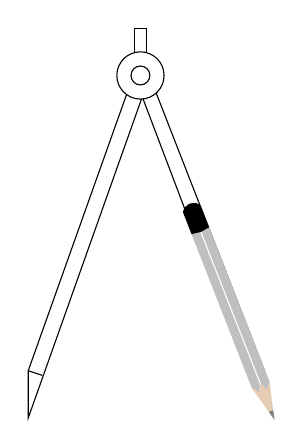
\begin{tikzpicture}
\begin{scope}[rotate=0,transform shape,scale=3]
\draw (2.95,3.7) rectangle (3,3.95);
\draw (2.92,3.68) -- (2.5,2.5) -- (2.5,2.3) -- (2.99,3.68);
\draw (3.5,2.5) -- (3.43,2.48) -- (2.975,3.68);
\draw (3.04,3.68) -- (3.5,2.5);
\draw (2.5,2.5) -- (2.56,2.48);
\draw[fill=white] (2.975,3.75) circle (0.1cm);
\draw (2.975,3.75) circle (0.04cm);
\end{scope}
\begin{scope}[xshift=10.34cm,yshift=7.28cm,rotate=21.4,scale=.6]          
\fill[gray!50] (0,4) -- (0.4,4) -- (0.4,0) --
               (0.3,-0.15) -- (0.2,0) -- (0.1,-0.14) --
               (0,0) -- cycle;
\draw[color=white] (0.2,4) -- (0.2,0);
\fill[black] (0,3.5) -- (0.2,3.47) -- (0.4,3.5) --
             (0.4,4) arc(30:150:0.23cm);
\fill[brown!40] (0,0) -- (0.2,-0.8)
    node[coordinate,pos=0.75](a){} -- 
    (0.4,0)node[coordinate,pos=0.25](b){} -- 
    (0.3,-0.15) -- (0.2,0) -- (0.1,-0.14) -- cycle;
\fill[gray] (a) -- (0.2,-0.8) -- (b) -- cycle;
\end{scope}
\end{tikzpicture}
\caption{Un compás  fijo. Un brazo tiene una aguja que se coloca en el centro del círculo. Un lápiz fijado al otro brazo sirve para dibujar el círculo. Los brazos están unidos por una bisagra ajustada modo que la distancia entre los brazos (el radio del círculo) se mantiene incluso cuando el compás se levanta del papel.}\label{fig.fixed-compass}
\end{minipage}
\hfill
\begin{minipage}{.45\textwidth}
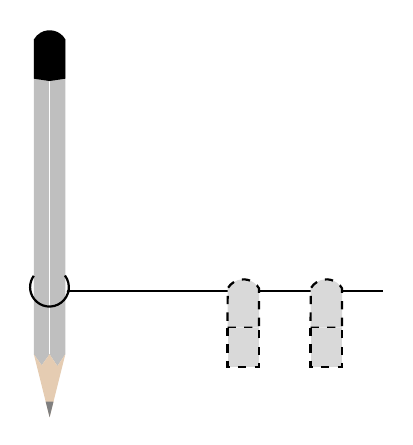
\begin{tikzpicture}[rotate=0,scale=1]          
\fill[gray!50] (0,4) -- (0.4,4) -- (0.4,0) --
               (0.3,-0.15) -- (0.2,0) -- (0.1,-0.14) --
               (0,0) -- cycle;
\draw[color=white] (0.2,4) -- (0.2,0);
\fill[black] (0,3.5) -- (0.2,3.47) -- (0.4,3.5) --
             (0.4,4) arc(30:150:0.23cm);
\fill[brown!40] (0,0) -- (0.2,-0.8)
    node[coordinate,pos=0.75](a){} -- 
    (0.4,0) node[coordinate,pos=0.25](b){} -- 
    (0.3,-0.15) -- (0.2,0) -- (0.1,-0.14) -- cycle;
\fill[gray] (a) -- (0.2,-0.8) -- (b) -- cycle;

\draw[thick] (0.395,1) arc (37:-216:7pt);
\coordinate (knot) at (0.44,.8);
\draw[thick] (knot) -- +(4,0);
\fill (knot) circle (.7pt);

\begin{scope}[xshift=100pt,yshift=-90pt]
\draw[dashed,thick,fill=white!70!gray] (0,3.5) -- (0.4,3.5) -- 
      (0.4,4) arc(30:150:0.23cm) -- cycle;
\draw[dashed,thick,fill=white!70!gray] (0,3.5) -- ++(0,-.5) -- ++(.4,0) -- ++(0,.5);
\end{scope}

\begin{scope}[xshift=70pt,yshift=-90pt]
\draw[dashed,thick,fill=white!70!gray] (0,3.5) -- (0.4,3.5) -- 
      (0.4,4) arc(30:150:0.23cm) -- cycle;
\draw[dashed,thick,fill=white!70!gray] (0,3.5) -- ++(0,-.5) -- ++(.4,0) -- ++(0,.5);
\end{scope}
\end{tikzpicture}
\caption{Un compás plegable. El usuario sujeta un trozo de cuerda en el centro del círculo. El otro extremo de la cuerda se ata a un lápiz y se utiliza para dibujar el círculo. Cuando se levanta el compás del papel, los dedos (punteados) pueden deslizarse fácilmente hasta una nueva posición.}\label{fig.collapsing-compass}
\end{minipage}
\end{figure}

Este capítulo comienza con una discusión sobre la relevancia de estudiar la construcción con regla y compás (Sec.~\ref{s.relevance}).
En el apartado~\ref{s.collapse} se comparan los dos tipos de compás en la construcción más elemental: una mediatriz. En el apartado~\ref{s.collapse-copy} se presenta el método de Euclides para copiar un segmento de recta utilizando un compás plegable. Esto demuestra que cualquier construcción que se pueda hacer usando un compás fijo se puede realizar usando un compás plegable. La sección~\ref{s.collapse-copy-incorrect} presenta una demostración de este teorema que parece correcta, pero no funciona para todas las configuraciones de rectas y puntos. Para enfatizar que no hay que fiarse de los diagramas, la sección~\ref{s.collapse-} presenta una famosa supuesta demostración de que todos los triángulos son ; la demostración parece correcta, pero no lo es porque se basa en un diagrama incorrecto.

\section{Construcción con regla y compás}\label{s.relevance}

La construcción con regla y compás solía ser el concepto fundamental que se enseñaba en geometría euclidiana. Recientemente, ha caído en desgracia en los programas escolares. Es cierto que el tema tiene poca o ninguna utilidad práctica. Como mostramos en las secciones~\ref{s.neusis}, \ref{s.neusis-doubling}, \ref{s.q}, \ref{s.square-quad}, los griegos sabían cómo realizar construcciones que son imposibles con una regla y un compás utilizando herramientas sólo ligeramente más avanzadas. Hoy en día, mediante métodos numéricos, los ordenadores pueden realizar construcciones con la precisión que se desee.

No obstante, creo que estudiar las construcciones tiene sus ventajas:
\begin{itemize}
\item Es más divertido y desafiante aprender geometría a través de construcciones que simplemente leyendo teoremas y demostraciones.
\item Se han logrado avances significativos en matemáticas mediante intentos de encontrar construcciones. El capítulo~\ref{c.heptadecagon} presenta una construcción de Gauss que condujo al álgebra abstracta moderna, en particular, la teoría desarrollada por \'{E}variste Galois.
\item Es algo contraintuitivo y por lo tanto muy interesante que se pueda demostrar que es imposible construir algunos objetos geométricos.
\item Lamentablemente, hay muchas personas que pierden años de su vida intentando realizar construcciones imposibles. Los estudiantes deberían ser conscientes de la inutilidad de tales esfuerzos.
\end{itemize}

\section{Compases fijos y compases plegables}\label{s.collapse}

Algunos libros de geometría presentan la construcción de la mediatriz de un segmento de recta construyendo dos circunferencias centradas en los extremos del segmento de forma que los radios sean iguales y mayores que la mitad de la longitud del segmento (Fig.~\ref{f.collapse-perp-bisector-fixed}). Esto sólo se puede hacer con un compás fijo porque después de dibujar el círculo centrado en $A$, la distancia entre los brazos del compás tiene que permanecer fija para dibujar el círculo centrado en $B$.

\begin{figure}[t]
\begin{minipage}{.45\textwidth}
\begin{center}
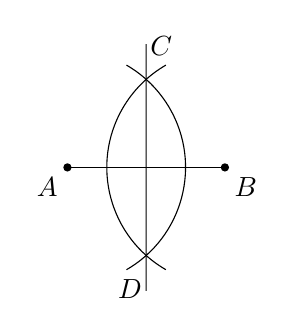
\begin{tikzpicture}[scale=0.5]
\coordinate (A) at (0,0);
\coordinate (B) at (4,0);
\vertex{A};
\vertex{B};
\draw (A) node[below left] {$A$} -- (B) node[below right] {$B$};
\draw[name path=larc] (A) ++(-60:3cm) arc (-60:60:3cm);
\draw[name path=rarc] (B) ++(-120:3cm) arc (-120:-240:3cm);
\path [name intersections={of=larc and rarc,by={b,t}}];
\node[above right,xshift=-2pt,yshift=5pt] at (t) {$C$};
\node[below left,xshift=2pt,yshift=-5pt] at (b) {$D$};
\draw ($ (b) ! 1.2 ! (t)$) -- ($ (t) ! 1.2 ! (b)$);
\end{tikzpicture}
\caption{Construcción de una mediatriz con compás fijo}\label{f.collapse-perp-bisector-fixed}
\end{center}
\end{minipage}
\hfill
\begin{minipage}{.45\textwidth}
\begin{center}
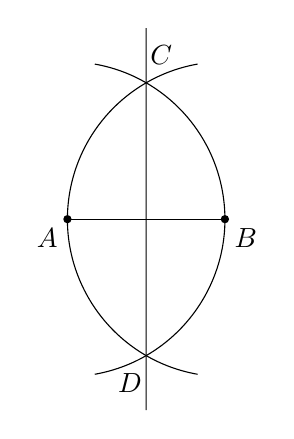
\begin{tikzpicture}[scale=0.5]
\coordinate (A) at (0,0);
\coordinate (B) at (4,0);
\vertex{A};
\vertex{B};
\draw (A) node[below left] {$A$} -- (B) node[below right] {$B$};
\draw[name path=larc] (A) ++(-80:4cm) arc (-80:80:4cm);
\draw[name path=rarc] (B) ++(-100:4cm) arc (-100:-260:4cm);
\path [name intersections={of=larc and rarc,by={b,t}}];
\node[above right,xshift=-2pt,yshift=3pt] at (t) {$C$};
\node[below left,xshift=2pt,yshift=-3pt] at (b) {$D$};
\draw ($ (b) ! 1.2 ! (t)$) -- ($ (t) ! 1.2 ! (b)$);
\end{tikzpicture}
\caption{Construcción de una mediatriz con compás fijo o plegable}\label{f.collapse-perp-bisector-collapse}
\end{center}
\end{minipage}
\end{figure}

Figura~\ref{f.collapse-perp-bisector-collapse} muestra la construcción de una mediatriz con compás fijo o con compás plegable. Se construyen dos circunferencias: una centrada en $A$ con radio $\overline{AB}$ y otra centrada en $B$ con radio $\overline{BA}$. Esto se puede hacer con un compás plegable porque (obviamente) $\overline{AB}=\overline{BA}$, por lo que el compás no tiene que ``recordar'' la longitud de $\overline{AB}$ para construir una circunferencia centrada en $B$ con el mismo radio.
La demostración de que la recta construida mostrada en la Fig.~\ref{f.collapse-perp-bisector-fixed} es una mediatriz no es nada elemental porque hay que utilizar conceptos relativamente avanzados como triángulos congruentes. Sin embargo, la demostración de que la construcción de una mediatriz mostrada en la Fig.~\ref{f.collapse-perp-bisector-collapse} es correcta es sencilla y se basa en el hecho de que $\triangle ABC$ es un triángulo equilátero. De hecho, esta es la primera proposición en los \textit{Elementos} de Euclides.
$\overline{AC}=\overline{AB}$ ya que son radios del mismo círculo, análogamente, $\overline{BC}=\overline{BA}$. Tenemos: $\overline{AC}=\overline{AB}=\overline{BA}=\overline{BC}$.

Figura~\ref{f.collapse-equilateral-fixed} muestra que para la construcción con compás fijo, el triángulo será un triángulo isósceles, no necesariamente equilátero (Fig.~\ref{f.collapse-equilateral-collapse}).

\section{Construcción de Euclides para copiar un segmento de recta}\label{s.collapse-copy}

La segunda proposición de los \textit{Elementos} de Euclides describe cómo copiar un segmento de recta $\overline{AB}$ dado un segmento de la misma longitud, uno de cuyos puntos extremos es un punto $C$ dado. Por lo tanto, un compás fijo no añade ninguna capacidad adicional y basta con un compás plegable, aunque las construcciones son más fáciles con un compás fijo.

\begin{theorem}
Dado un segmento de recta $\overline{AB}$ y un punto $C$, se puede construir un segmento de recta $\overline{CC'}$, uno de cuyos puntos extremos es $C$, utilizando un compás plegable, tal que $\overline{AB}=\overline{CC'}$ (Fig.~\ref{f.collapse-copying-1}).
\end{theorem}

\begin{figure}[t]
\begin{minipage}{.45\textwidth}
\begin{center}
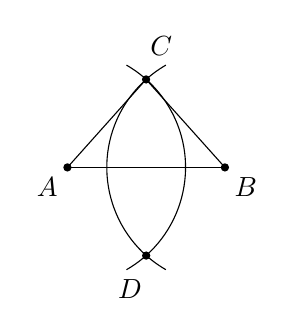
\begin{tikzpicture}[scale=0.5]
\coordinate (A) at (0,0);
\coordinate (B) at (4,0);
\vertex{A};
\vertex{B};
\draw (A) node[below left] {$A$} -- (B) node[below right] {$B$};
\draw[name path=larc] (A) ++(-60:3cm) arc (-60:60:3cm);
\draw[name path=rarc] (B) ++(-120:3cm) arc (-120:-240:3cm);
\path [name intersections={of=larc and rarc,by={b,t}}];
\vertex{t};
\vertex{b};
\node[above right,xshift=-2pt,yshift=5pt] at (t) {$C$};
\node[below left,xshift=2pt,yshift=-5pt] at (b) {$D$};
\draw (A) -- (t);
\draw (B) -- (t);
\end{tikzpicture}
\caption{Construcción de un triángulo isóceles con compás fijo}\label{f.collapse-equilateral-fixed}
\end{center}
\end{minipage}
\hfill
\begin{minipage}{.45\textwidth}
\begin{center}
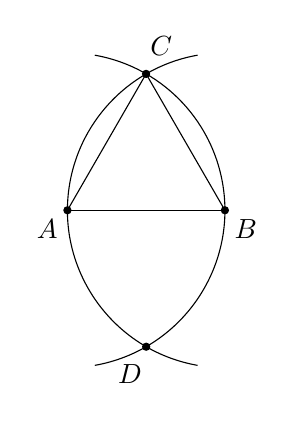
\begin{tikzpicture}[scale=0.5]
\coordinate (A) at (0,0);
\coordinate (B) at (4,0);
\draw (A) node[below left] {$A$} -- (B) node[below right] {$B$};
\vertex{A};
\vertex{B};
\draw[name path=larc] (A) ++(-80:4cm) arc (-80:80:4cm);
\draw[name path=rarc] (B) ++(-100:4cm) arc (-100:-260:4cm);
\path [name intersections={of=larc and rarc,by={b,t}}];
\vertex{t};
\vertex{b};
\node[above right,xshift=-2pt,yshift=3pt] at (t) {$C$};
\node[below left,xshift=2pt,yshift=-3pt] at (b) {$D$};
\draw (A) -- (t);
\draw (B) -- (t);
\end{tikzpicture}
\caption{Construcción de un triángulo equilátero con un compás plegable}\label{f.collapse-equilateral-collapse}
\end{center}
\end{minipage}
\end{figure}

\begin{figure}[b]
\begin{minipage}{.45\textwidth}
\begin{center}
\begin{tikzpicture}[scale=0.5]
\coordinate (C) at (0,0);
\coordinate (A) at (3,0);
\draw (A) node[below,xshift=-2pt,yshift=-2pt] {$A$} -- +(40:4) coordinate (B) node[right] {$B$};
\vertex{A};
\vertex{B};
\vertex{C};
\node[below,xshift=2pt,yshift=-2pt] at (C) {$C$};
\draw[thick,dashed] (C) -- +(160:4) coordinate (D) node[below] {$C'$};
\vertex{D};
\end{tikzpicture}
\caption{Copiar el segmento de recta $\overline{AB}$. La orientación de $\overline{CC'}$ no es importante.}\label{f.collapse-copying-1}
\end{center}
\end{minipage}
\hfill
\begin{minipage}{.45\textwidth}
\begin{center}
\begin{tikzpicture}[scale=0.5]
\coordinate (C) at (0,0);
\coordinate (A) at (3,0);
\draw (A) node[below,xshift=-2pt,yshift=-2pt] {$A$} -- +(40:4) coordinate (B) node[right] {$B$};
\vertex{B};
\node[below,xshift=2pt,yshift=-2pt] at (C) {$C$};
\draw (A) -- (C);
\path[name path=larc] (C) ++(-70:2.5cm) arc (-70:70:2.5cm);
\path[name path=rarc] (A) ++(-110:2.5cm) arc (-110:-250:2.5cm);
\path [name intersections={of=larc and rarc,by={d,D}}];
\node[above] at (D) {$D$};
\draw (A) -- (D);
\draw (C) -- (D);
\end{tikzpicture}
\caption{Copiar un segmento de línea con un compás plegable}\label{f.collapse-copying-2}
\end{center}
\end{minipage}
\end{figure}

\begin{proof}
Construimos el segmento de recta $\overline{AC}$. Construimos el triángulo equilátero $\triangle ACD$ cuya base es $\overline{AC}$ (Fig.~\ref{f.collapse-copying-2}). Por la primera proposición de Euclides, el triángulo se puede construir utilizando un compás plegable. Construimos la semirrecta que es prolongación del segmento \emph{de $D$ a $A$}, y construir la semirrecta que es prolongación de la recta segmento \emph{de $D$ a $C$} (Fig.~\ref{f.collapse-copying-3}). Construimos la circunferencia centrada en $A$ con radio $\overline{AB}$ y denotamos con E la intersección de la circunferencia y la semirrecta que prolonga $\overline{DA}$ (Fig.~\ref{f.collapse-copying-4}). Construimos la circunferencia centrada en $D$ con radio $\overline{DE}$ y denotamos con $F$ la intersección de la circunferencia y la semirrecta que prolonga $\overline{DC}$ (Fig.~\ref{f.collapse-copying-5}).

\begin{figure}[t]
\begin{minipage}{.45\textwidth}
\begin{center}
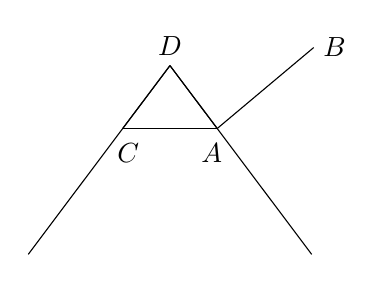
\begin{tikzpicture}[scale=0.4]
\coordinate (C) at (0,0);
\coordinate (A) at (3,0);
\draw (A) node[below,xshift=-2pt,yshift=-2pt] {$A$} -- +(40:4) coordinate (B) node[right] {$B$};
\node[below,xshift=2pt,yshift=-2pt] at (C) {$C$};
\draw (A) -- (C);
\path[name path=larc] (C) ++(-70:2.5cm) arc (-70:70:2.5cm);
\path[name path=rarc] (A) ++(-110:2.5cm) arc (-110:-250:2.5cm);
\path [name intersections={of=larc and rarc,by={d,D}}];
\node[above] at (D) {$D$};
\draw (A) -- (D);
\draw (C) -- (D);
\draw[name path=ray2] (D) -- ($ (D) ! 3 ! (C) $);
\draw[name path=ray1] (D) -- ($ (D) ! 3 ! (A) $);
\end{tikzpicture}
\caption{Construcción de semirrectas a partir de $D$}\label{f.collapse-copying-3}
\end{center}
\end{minipage}
\hfill
\begin{minipage}{.45\textwidth}
\begin{center}
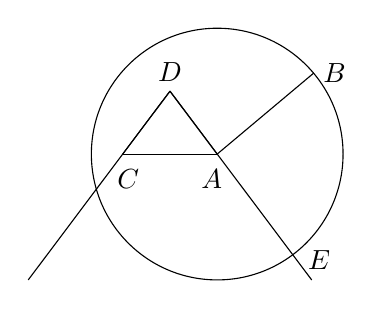
\begin{tikzpicture}[scale=0.4]
\coordinate (C) at (0,0);
\coordinate (A) at (3,0);
\draw (A) node[below,xshift=-2pt,yshift=-2pt] {$A$} -- +(40:4) coordinate (B) node[right] {$B$};
\node[below,xshift=2pt,yshift=-2pt] at (C) {$C$};
\draw (A) -- (C);
\path[name path=larc] (C) ++(-70:2.5cm) arc (-70:70:2.5cm);
\path[name path=rarc] (A) ++(-110:2.5cm) arc (-110:-250:2.5cm);
\path [name intersections={of=larc and rarc,by={d,D}}];
\node[above] at (D) {$D$};
\draw (A) -- (D);
\draw (C) -- (D);
\draw[name path=ray2] (D) -- ($ (D) ! 3 ! (C) $);
\draw[name path=ray1] (D) -- ($ (D) ! 3 ! (A) $);
\node[draw,circle through=(B),name path=c1] at (A) {};
\path [name intersections={of=c1 and ray1,by={E,e}}];
\node[right,xshift=2pt,yshift=-2pt] at (E) {$E$};
\end{tikzpicture}
\caption{Construimos un círculo de radio $\overline{AB}$}\label{f.collapse-copying-4}
\end{center}
\end{minipage}
\end{figure}

$\overline{DC}=\overline{DA}$ porque el $\triangle ACD$ es equilátero. $\overline{AE}=\overline{AB}$ son radios de lamisma circunferencia, al igual que $\overline{DF}=\overline{DE}$. Por lo tanto:
\[
\overline{CF}=\overline{DF}-\overline{DC}=\overline{DE}-\overline{DC}=\overline{DE}-\overline{DA}=\overline{AE}=\overline{AB}\,.
\]
\end{proof}

\begin{figure}[b]
\begin{center}
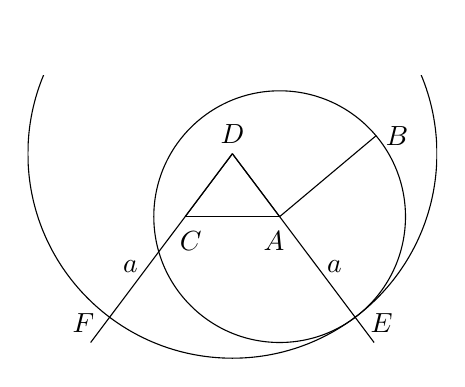
\begin{tikzpicture}[scale=0.4]
\clip (-5,-4.5) rectangle (8,6);
\coordinate (C) at (0,0);
\coordinate (A) at (3,0);
\draw (A) node[below,xshift=-2pt,yshift=-2pt] {$A$} -- +(40:4) coordinate (B) node[right] {$B$};
\node[below,xshift=2pt,yshift=-2pt] at (C) {$C$};
\draw (A) -- (C);
\path[name path=larc] (C) ++(-70:2.5cm) arc (-70:70:2.5cm);
\path[name path=rarc] (A) ++(-110:2.5cm) arc (-110:-250:2.5cm);
\path [name intersections={of=larc and rarc,by={d,D}}];
\node[above] at (D) {$D$};
\draw (A) -- (D);
\draw (C) -- (D);
\draw[name path=ray2] (D) -- ($ (D) ! 3 ! (C) $);
\draw[name path=ray1] (D) -- ($ (D) ! 3 ! (A) $);
\node[draw,circle through=(B),name path=c1] at (A) {};
\path [name intersections={of=c1 and ray1,by={E,e}}];
\node[right,xshift=2pt,yshift=-2pt] at (E) {$E$};
\node[draw,circle through=(E),name path=c2] at (D) {};
\path [name intersections={of=c2 and ray2,by={F,f}}];
\node[left,xshift=-2pt,yshift=-2pt] at (F) {$F$};
\path (A) -- node[right] {$a$} (E);
\path (C) -- node[left] {$a$} (F);
\draw[white,fill=white] (-5,4.5) rectangle +(13,1.5);
\end{tikzpicture}
\end{center}
\caption{Construcción de $\overline{CF}=\overline{AB}$}\label{f.collapse-copying-5}
\end{figure}

La especificación de las direcciones de las semirrectas es esencial. La demostración funciona para cualquier segmento de recta $\overline{AB}$ y cualquier punto $C$, independientemente de su posición respecto a $\overline{AB}$.  Especificando las direcciones, el ``cono'' encerrado por los dos rayos intersecará los círculos aunque $\overline{AC}>\overline{AB}$ (Fig.~\ref{f.collapse-copying-6}).

\begin{figure}
\begin{center}
\begin{tikzpicture}[scale=0.4]
\clip (-12,-6) rectangle (11,10);
\coordinate (C) at (-4,0);
\coordinate (A) at (3,0);
\draw (A) node[below,xshift=-2pt,yshift=-2pt] {$A$} -- +(40:4) coordinate (B) node[right] {$B$};
\node[below,xshift=2pt,yshift=-2pt] at (C) {$C$};
\draw (A) -- (C);
\path[name path=larc] (C) ++(-70:7cm) arc (-70:70:7cm);
\path[name path=rarc] (A) ++(-110:7cm) arc (-110:-250:7cm);
\path [name intersections={of=larc and rarc,by={d,D}}];
\node[above] at (D) {$D$};
\draw (A) -- (D);
\draw (C) -- (D);
\draw[name path=ray2] (D) -- ($ (D) ! 2 ! (C) $);
\draw[name path=ray1] (D) -- ($ (D) ! 2 ! (A) $);
\node[draw,circle through=(B),name path=c1] at (A) {};
\path [name intersections={of=c1 and ray1,by={e,E}}];
\node[right,xshift=2pt,yshift=-2pt] at (E) {$E$};
\node[draw,circle through=(E),name path=c2] at (D) {};
\path [name intersections={of=c2 and ray2,by={F,f}}];
\node[left,xshift=-2pt,yshift=-2pt] at (F) {$F$};
\path (A) -- node[right] {$a$} (E);
\path (C) -- node[left] {$a$} (F);
\draw[white,fill=white] (-12,8) rectangle +(23,2);
\end{tikzpicture}
\end{center}
\caption{Construcción para $\overline{AC}>\overline{AB}$}\label{f.collapse-copying-6}
\end{figure}

%%%%%%%%%%%%%%%%%%%%%%%%%%%%%%%%%%%%%%%%%%%%%%%%%%%%%%%%%%%%%%%

\section{Una construcción errónea para copiar un segmento de línea}\label{s.collapse-copy-incorrect}

\begin{proof}
Construimos tres circunferencias: una centrada en $A$ con radio $\overline{AB}$, otra centrada en $A$ con radio $\overline{AC}$, y otra centrada en $C$ con radio $\overline{AC}=\overline{CA}$. Denotamos las intersecciones de las circunferencias centradas en $A$ y $C$ con $E$ y $F$, respectivamente, y denotamos una intersección de la circunferencia centrada en $C$ y la circunferencia centrada en $A$ con radio $\overline{AB}$ con $D$. Si $\overline{AC}>\overline{AB}$, la construcción es como se muestra en Fig.~\ref{f.collapse-incorrect-1}.
\begin{figure}[b]
\begin{center}
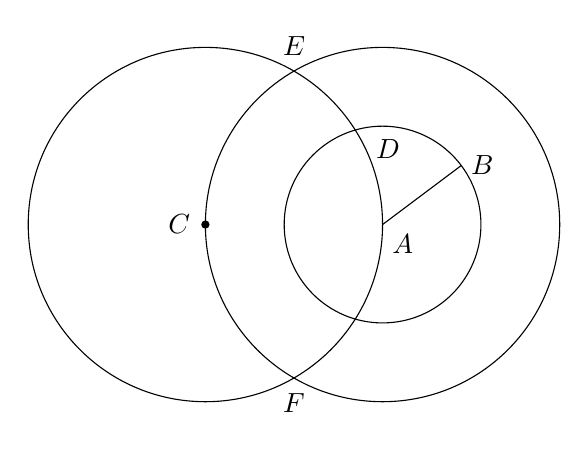
\begin{tikzpicture}[scale=0.5]
\coordinate (C) at (-2,0);
\coordinate (A) at (2.5,0);
\coordinate (B) at (4.5,1.5);
\draw (A) node[below right] {$A$} -- (B) node[right] {$B$};
\node[left,xshift=-2pt] at (C) {$C$};
\node[draw,circle through=(B),name path=c1] at (A) {};
\node[draw,circle through=(C),name path=c2] at (A) {};
\node[draw,circle through=(A),name path=c3] at (C) {};
\path [name intersections={of=c1 and c3,by={D,f}}];
\path [name intersections={of=c2 and c3,by={E,F}}];
\node[below right,xshift=4pt] at (D) {$D$};
\node[above,yshift=2pt] at (E) {$E$};
\node[below,yshift=-2pt] at (F) {$F$};
\vertex{C};
\end{tikzpicture}
\end{center}
\caption{Construcción para copiar un segmento de recta (1)}\label{f.collapse-incorrect-1}
\end{figure}

\begin{figure}[t]
\begin{center}
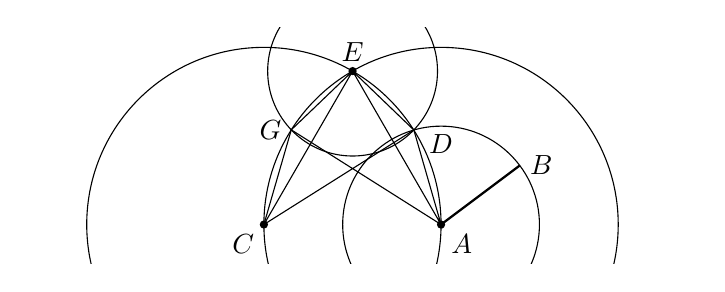
\begin{tikzpicture}[scale=0.5]
\clip (-8,-1) rectangle (9,5);
\coordinate (C) at (-2,0);
\coordinate (A) at (2.5,0);
\coordinate (B) at (4.5,1.5);
\draw[thick] (A) node[below right] {$A$} -- (B) node[right] {$B$};
\vertex{A};
\vertex{C};
\node[below left] at (C) {$C$};
\node[draw,circle through=(B),name path=c1] at (A) {};
\node[draw,circle through=(C),name path=c2] at (A) {};
\node[draw,circle through=(A),name path=c3] at (C) {};
\path [name intersections={of=c1 and c3,by={D,f}}];
\path [name intersections={of=c2 and c3,by={E,F}}];
\node[draw,circle through=(D),name path=c4] at (E) {};
\path [name intersections={of=c2 and c4,by={g,G}}];
\node[left] at (G) {$G$};
\node[below right,yshift=2pt,xshift=2pt] at (D) {$D$};
\node[above] at (E) {$E$};
\vertex{E};
\vertex{F};
\draw (C) -- (G);
\draw (A) -- (G) -- (E) -- (C) -- (D);
\draw (A) -- (D) -- (E) -- cycle;
\end{tikzpicture}
\end{center}
\caption{Construcción para copiar un segmento de recta (2)}\label{f.collapse-incorrect-2}
\end{figure}

Construimos una circunferencia centrada en $E$ con radio $\overline{ED}$. Denotemos por $G$ la intersección de esta circunferencia con la circunferencia centrada en $A$ de radio $\overline{AC}$. Hay dos intersecciones, por lo que elegir la más cercana a $C$ (Fig.~\ref{f.collapse-incorrect-2}).
$\overline{CD}=\overline{CE}$ son radios de la misma circunferencia que $\overline{AE}=\overline{AG}$. Por construcción los radios $\overline{CE}$ y $\overline{AE}$ son iguales. Por tanto:
\[
\overline{CD} = \overline{CE} = \overline{AE} = \overline{AG}\,.
\]
$\overline{EG} = \overline{ED}$ son radios del mismo círculo, por lo que $\triangle EAG\cong \triangle DCE$ por lado-lado-lado y $\angle GEA = \angle DEC$.

Como:
\[
\angle GEC = \angle GEA \!-\!\angle CEA = \angle DEC\!-\!\angle CEA = \angle DEA\,,
\]
resulta que $\triangle ADE\cong\triangle CGE$ por lado-ángulo-lado. $\overline{AB}=\overline{AD}$ son radios del círculo menor centrado en $A$, por lo que $\overline{GC}=\overline{AD}=\overline{AB}$.
\end{proof}

La demostración sólo es correcta si $\overline{AC}>\overline{AB}$.  Figura~\ref{f.collapse-incorrect-4} muestra un diagrama donde $\overline{AC}<\overline{AB}$ y se puede ver que $\overline{AB}\neq\overline{GC}$.

\begin{figure}[b]
\begin{center}
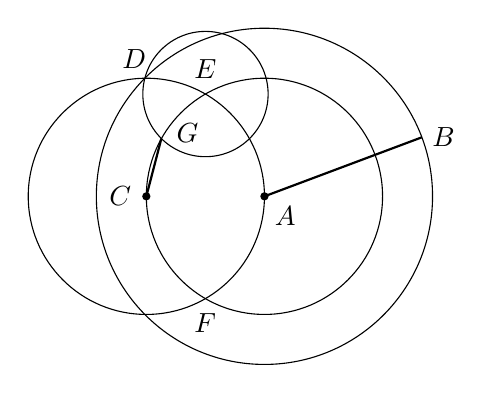
\begin{tikzpicture}[scale=0.5]
\coordinate (C) at (-1,0);
\coordinate (A) at (2,0);
\coordinate (B) at (6,1.5);
\draw[thick] (A) node[below right] {$A$} -- (B) node[right] {$B$};
\node[left,xshift=-2pt] at (C) {$C$};
\node[draw,circle through=(B),name path=c1] at (A) {};
\node[draw,circle through=(C),name path=c2] at (A) {};
\node[draw,circle through=(A),name path=c3] at (C) {};
\path [name intersections={of=c1 and c3,by={D,f}}];
\path [name intersections={of=c2 and c3,by={E,F}}];
\node[above left,xshift=4pt] at (D) {$D$};
\node[above,yshift=2pt] at (E) {$E$};
\node[below,yshift=-2pt] at (F) {$F$};
\vertex{A};
\vertex{C};
\node[draw,circle through=(D),name path=c4] at (E) {};
\path [name intersections={of=c2 and c4,by={g,G}}];
\node[right,xshift=2pt,yshift=2pt] at (G) {$G$};
\draw[thick] (G) -- (C);
\end{tikzpicture}
\end{center}
\caption{Un diagrama para el que la demostración no funciona}\label{f.collapse-incorrect-4}
\end{figure}


\section{No te fíes de un diagrama}\label{s.collapse-}

\begin{theorem}[Incorrecto, por supuesto]
Todos los triángulos son isósceles.
\end{theorem}\index{Triangle!@all are }

\begin{proof}
Dado un triángulo arbitrario $\triangle ABC$, sea $P$ la intersección de la bisectriz del ángulo $\angle BAC$ y la mediatriz de $\overline{BC}$. Las intersecciones de las altitudes desde $P$ a los lados $\overline{AB}$, $\overline{AC}$ se denotan por $E,F$, respectivamente (Fig.~\ref{f.collapse--1}). 
\begin{figure}[t]
\begin{center}
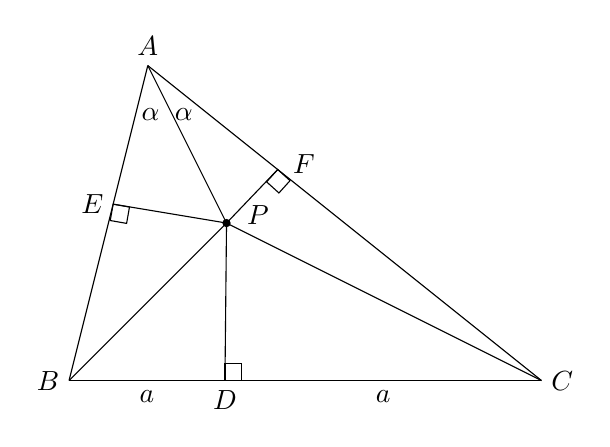
\begin{tikzpicture}[scale=1]
\coordinate (P) at (0,0);
\node[xshift=4mm,yshift=1mm] at (P) {$P$};
\coordinate [label=left:$B$] (B)  at (-2,-2);
\coordinate [label=right:$C$] (C)  at (4,-2);
\coordinate [label=above:$A$] (A)  at (-1,2);
\node[below,yshift=-12pt,xshift=1pt] at (A) {$\alpha$};
\node[below,yshift=-12pt,xshift=13pt] at (A) {$\alpha$};
\draw (A) -- (B);
\draw (A) -- (C);
\draw (B) -- (C);
\draw (A) -- (P);
\draw (B) -- (P);
\draw (C) -- (P);
\coordinate[label=left:$E$] (E) at ($ (A) ! .44 ! (B) $);
\draw[rotate=-100] (E) rectangle +(6pt,6pt);
\draw (P) -- (E);
\coordinate (F) at ($ (A) ! .33 ! (C) $);
\node[right,xshift=2pt,yshift=2pt] at (F) {$F$};
\draw[rotate=-132] (F) rectangle +(6pt,6pt);
\draw (P) -- (F);
\coordinate[label=below:$D$] (D) at ($ (B) ! .33 ! (C) $);
\draw (D) rectangle +(6pt,6pt);
\draw (P) -- (D);
\node[left] at ($ (A) ! .5 ! (E) $) {};
\node[left] at ($ (B) ! .5 ! (E) $) {};
\node[below] at ($ (B) ! .5 ! (D) $) {$a$};
\node[below] at ($ (C) ! .5 ! (D) $) {$a$};
\node[right,xshift=2pt] at ($ (A) ! .5 ! (F) $) {};
\node[right,xshift=2pt] at ($ (C) ! .5 ! (F) $) {};
\vertex{P};
\end{tikzpicture}
\end{center}
\caption{Una demostración incorrecta de que todos los triángulos son isóceles}\label{f.collapse--1}
\end{figure}
$\triangle APE\cong \triangle APF$ porque son triángulos rectángulos con ángulos iguales $\alpha$ y lado común $\overline{AP}$. $\triangle DPB\cong \triangle DPC$ ya que son triángulos rectángulos, $\overline{PD}$ es un lado común y $\overline{BD}=\overline{CD}=a$. $\triangle EPB\cong \triangle FPC$ ya que son triángulos rectángulos, $\overline{EP}=\overline{PF}$ por la primera congruencia y $\overline{PB}=\overline{PC}$ por la segunda congruencia. Combinando las ecuaciones obtenemos que $\triangle ABC$ es :
\[
\overline{AB}= \overline{AE}+\overline{EB}=\overline{AF}+\overline{FC} =\overline{AC}\,.
\]
\end{proof}

La lógica de la demostración es correcta, pero el diagrama en el que se basa la demostración no es correcto porque el punto $P$ está fuera del triángulo. (Fig.~\ref{f.collapse--2}).

\begin{figure}[b]
\begin{center}
\begin{tikzpicture}[scale=.5]
\coordinate (B) at (0,0);
\coordinate (C) at (8,0);
\path[name path=ba] (B) -- +(70:6);
\path[name path=ca] (C) -- +(140:8.5);
\path [name intersections={of=ba and ca,by={A}}];
\draw (B) -- (C) -- (A) -- cycle;
\node[above] at (A) {$A$};
\node[below,yshift=-12pt,xshift=-1pt] at (A) {$\alpha$};
\node[below right,xshift=5pt,yshift=-12pt] at (A) {$\alpha$};
\node[left] at (B) {$B$};
\node[right] at (C) {$C$};
\draw[name path=angle] (A) -- +(-75:9);
\draw ($(B)!.5!(C)$) -- +(0,3);
\draw[name path=perp] ($(B)!.5!(C)$) -- +(0,-3.5);
\path [name intersections={of=angle and perp,by={X}}];
\vertex{X};
\draw (4,0) rectangle +(10pt,10pt);
\node[right] at (X) {$P$};
\end{tikzpicture}
\caption{Por qué no funciona la construcción}\label{f.collapse--2}
\end{center}
\end{figure}

\subsection*{¿Cuál es la sorpresa?}

De estudiante daba por sentado que un compás tiene una bisagra que mantiene la distancia entre la punta y el lápiz cuando se levanta del papel. Cuando el profesor utilizaba un compás hecho con un trozo de cuerda y un trozo de tiza, nunca imaginé que se diferenciara de mi compás. El artículo de Gotfried Toussaint fue una verdadera sorpresa, al igual que su demostración de que las demostraciones posteriores a Euclides eran incorrectas porque dependían de diagramas que hacían suposiciones injustificadas. Recomiendo el artículo a los lectores que deseen profundizar en el conocimiento de las demostraciones en matemáticas.

\subsection*{Fuentes}

Este capítulo se basa en \cite{toussaint}. La construcción incorrecta de la equivalencia de los dos compases en Sect.~\ref{s.collapse-copy-incorrect} es de \cite{rusty}. Thomas L. Heath, uno de los mayores expertos en matemáticas griegas, ha escrito una exhaustiva traducción al inglés de los \textit{Elements} de Euclides junto con un extenso comentario \cite{euclid}.


\tikzsetfigurename{trisect}
% !TeX root = surprises.tex

\chapter{Trisection of an Angle}\label{c.trisect}

%%%%%%%%%%%%%%%%%%%%%%%%%%%%%%%%%%%%%%%%%%%%%%%%%%%%%%%%%%%%%%%

\abstract*{It is impossible to trisect an angle using only a straightedge and compass. This was proved in by Pierre Wantzel in 1837. Nevertheless, innumerable amateurs continue to attempt to trisect an angle. This chapter presents two incorrect constructions and through trigonometry shows that the constructions are approximations.
The Greeks discovered that if other instruments are allowed, angles can be trisected. We bring Archimedes's construct using a simple instrument called a neusis and a more complex construction by Hippias using the quadratrix.
The rest of the chapter contains a somewhat informal proof of the impossibility of trisecting an angle by characterizing constructible numbers and then relating them constructible numbers to roots of polynomials which proves the impossibility.}

%%%%%%%%%%%%%%%%%%%%%%%%%%%%%%%%%%%%%%%%%%%%%%%%%%%%%%%%%%%%%%%

It is impossible to trisect an arbitrary angle (divide the angle into three equal parts) using only a straightedge and compass. Trisection requires the construction of cube roots, but a straightedge and compass can only construct lengths that are expressions built from integers, the four arithmetic operators and square roots. This was proved by Pierre Wantzel\index{Wantzel, Pierre} in 1837. Nevertheless, innumerable amateurs continue to attempt to trisect an angle. Their constructions are approximations though they are convinced that the constructions are correct. Section~\ref{s.trisect-approx} presents two such constructions, develops formulas for the angles and shows the errors in the approximations.

Greek mathematicians discovered that if other instruments are allowed, angles can be trisected. Section~\ref{s.neusis} explains a construction by Archimedes\index{Archimedes} using a simple instrument called a \emph{neusis} and Sect~\ref{s.neusis-doubling} shows how to double a cube using the neusis. Section~\ref{s.q} presents a construction for trisection by Hippias\index{Hippias} using an instrument called a \emph{quadratrix}. The rest of the chapter contains a proof of the impossibility of trisecting an angle. Section~\ref{s.trisect-constructible} characterizes constructible numbers, Sect.~\ref{s.trisect-poly} relates constructible numbers to roots of polynomials and Sect.~\ref{s.trisect-impossible} uses this theory to show that trisecting an angle and doubling a cube are impossible.

%%%%%%%%%%%%%%%%%%%%%%%%%%%%%%%%%%%%%%%%%%%%%%%%%%%%%%%%

\section{Approximate Trisections}\label{s.trisect-approx}

\subsection{First Approximate Trisection}\index{Trisection of an angle!approximation}\label{sub.trisect-approx1}

\noindent\textbf{Construction:}
Let $\theta=\angle AOB$ be an arbitrary angle and without loss of generality assume that $A,B$ are on a unit circle whose center is $O$. Bisect $\angle AOB$ and let $C$ be the intersection of the bisector with the unit circle. Let $D$ be the midpoint of $\overline{OA}$ and let $T$ be the midpoint of the $\overline{DC}$. Denote the angle $\angle DOT$ by $\phi$ (Fig.~\ref{f.trisect-first-approx-1}).

\newpage

\begin{figure}[ht]
\begin{center}
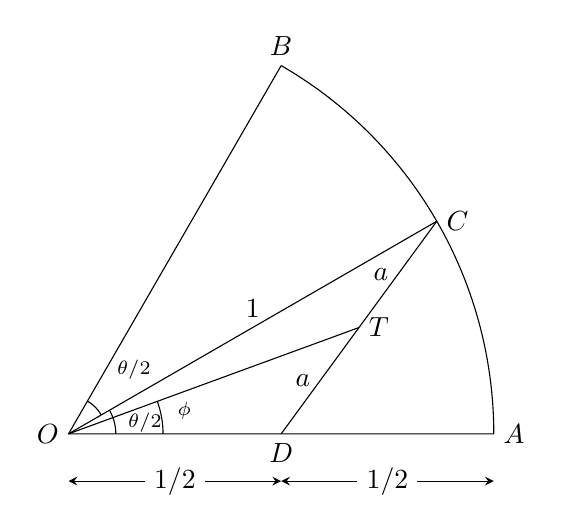
\begin{tikzpicture}[scale=.6]
\coordinate (O) at (0,0)
  node[left] {$O$}
  node[above right,xshift=14pt,yshift=16pt] {\sm{\theta/2}}
  node[right,xshift=18pt,yshift=4pt] {\sm{\theta/2}};
\coordinate (A) at (9cm,0);
\node[right] at (A) {$A$};
\coordinate (B) at (60:9);
\node[above] at (B) {$B$};
\draw (A) arc(0:60:9);
\draw (B) -- (O) -- (A);
\coordinate (C) at (30:9);
\node[right] at (C) {$C$};
\draw (O) -- node[above] {$1$} (C);
\coordinate (D) at (4.5,0);
\node[below] at (D) {$D$};
\coordinate (T) at ($(D)!.5!(C)$);
\draw (D) -- node[left] {$a$} (T) -- node[left] {$a$} (C);
\node[right] at (T) {$T$};
\draw (O) -- (T);
\draw (	1,0) arc (0:30:1);
\draw (30:.8) arc (30:60:.8);
\draw (2,0) arc (0:20:2);
\node[above right] at (2.1,0.1) {\sm{\phi}}; 

\draw[<->] (0,-1) -- node[fill=white] {$1/2$} +(4.5,0);
\draw[<->] (4.5,-1) -- node[fill=white] {$1/2$} +(4.5,0);
\end{tikzpicture}
\end{center}
\caption{First approximate trisection (1)}\label{f.trisect-first-approx-1}
\end{figure}


\begin{theorem}
\[\tan\phi =\frac{2\sin(\theta/2)}{1+2\cos(\theta/2)}\,.\]
\end{theorem}

\begin{proof} Figure~\ref{f.trisect-first-approx-2} is extracted from Fig.~\ref{f.trisect-first-approx-1} and contains additional annotations.

Let $\overline{CF}$ be the perpendicular to $\overline{OA}$ that intersects $\overline{OA}$ at $F$. Since $\overline{OC}=1$, $\overline{CF}=\sin (\theta/2)$ and $\overline{OF}=\cos(\theta/2)$. Let $\overline{TE}$ be the perpendicular to $\overline{OA}$ that intersects $\overline{OA}$ at $E$.

$T$ is the midpoint of $\overline{DC}$ so $\overline{DT}=\overline{TC}=a$. But $\overline{FT}$ is the median to the hypotenuse of a right triangle, so $\overline{FT}=a$ and therefore $\triangle DTF$ is isoceles. It follows that $\overline{TE}$ is the both the median and the altitude of $\overline{DF}$. From the diagram it is easy to see that:
\begin{figure}[ht]
\begin{center}
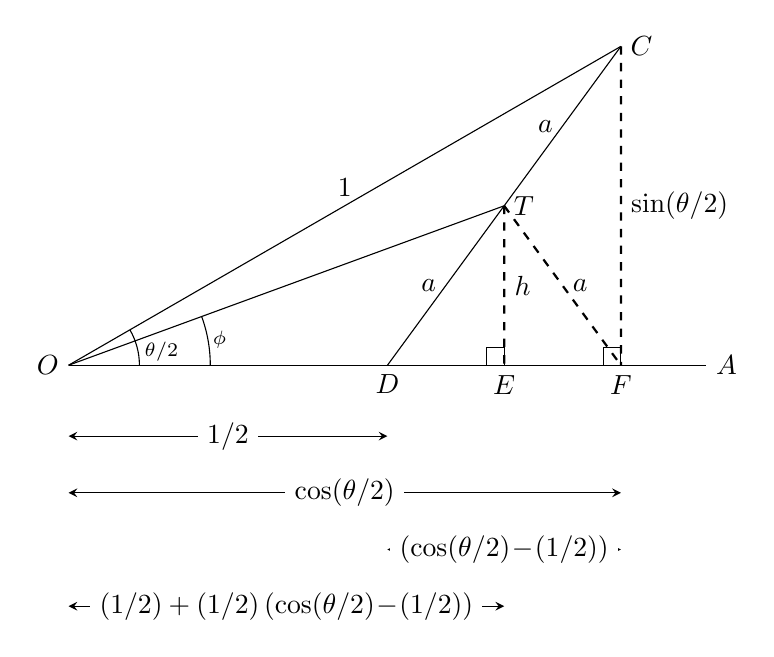
\begin{tikzpicture}[scale=.9]
\coordinate (O) at (0,0)
  node[left] {$O$}
  node[right,xshift=24pt,yshift=5pt] {\sm{\theta/2}};
\coordinate (A) at (9cm,0);
\node[right] at (A) {$A$};
\draw (O) -- (A);
\coordinate (C) at (30:9);
\node[right] at (C) {$C$};
\draw (O) -- node[above] {$1$} (C);
\coordinate (D) at (4.5,0);
\node[below] at (D) {$D$};
\coordinate (T) at ($(D)!.5!(C)$);
\draw (D) -- node[left] {$a$} (T) -- node[left] {$a$} (C);
\node[right] at (T) {$T$};
\draw (O) -- (T);
\draw (	1,0) arc (0:30:1);
\draw (2,0) arc (0:20:2);
\node[above right] at (1.9,0.1) {\sm{\phi}}; 

\coordinate (E) at (T |- A);
\draw[thick,dashed] (T) -- node[right] {$h$}
  (E) node[below] {$E$};
\draw[rotate=90] (E) rectangle +(7pt,7pt);

\coordinate (F) at (C |- A);
\draw[thick,dashed] (C) --
  node[right] {$\sin (\theta/2)$} (F) node[below] {$F$};
\draw[rotate=90] (F) rectangle +(7pt,7pt);

\draw[thick,dashed] (T) -- node[right] {$a$} (F);

\draw[<->] ($(O)+(0,-1)$) --
  node[fill=white] {$1/2$} +(4.5,0);
\draw[<->] ($(O)+(0,-1.8)$) --
  node[fill=white] {$\cos (\theta/2)$} ($(F)+(0,-1.8)$);
\draw[<->] ($(D)+(0,-2.6)$) --
  node[fill=white] {$\left(\cos (\theta/2)\!-\! (1/2)\right)$} 
  ($(F)+(0,-2.6)$);
\draw[<->] ($(O)+(0,-3.4)$) --
  node[fill=white] {$(1/2)+(1/2)\left(\cos (\theta/2)\! -\! (1/2)\right)$} 
  ($(E)+(0,-3.4)$);
\end{tikzpicture}
\end{center}
\caption{First approximate trisection (2)}\label{f.trisect-first-approx-2}
\end{figure}
\[
\overline{OE}=\frac{1}{2} + \frac{1}{2}\left(\cos \frac{\theta}{2}-\frac{1}{2}\right)\,.
\]
Compute the length $2a=\overline{CD}$ using Pythagoras's Theorem in $\triangle DCF$:
\begin{eqnarray*}
(2a)^2 &=&  \left(\cos \frac{\theta}{2}-\frac{1}{2}\right)^2+\sin^2\frac{\theta}{2}\,.
\end{eqnarray*}

\newpage

The length $h=\overline{TE}$ can be computed from Pythagoras's Theorem in $\triangle DTE$:
\begin{eqnarray*}
a^2 &=& h^2 + \left[\frac{1}{2}\left(\cos \frac{\theta}{2}-\frac{1}{2}\right)\right]^2\\
h^2&=&\frac{1}{4}\left(\cos \frac{\theta}{2}-\frac{1}{2}\right)^2+\frac{1}{4}\sin^2\frac{\theta}{2}-\left[\frac{1}{2}\left(\cos \frac{\theta}{2}-\frac{1}{2}\right)\right]^2=
\frac{1}{4}\sin^2\frac{\theta}{2}\\
h&=&\frac{1}{2}\sin\frac{\theta}{2}\\
\tan\phi &=&\frac{h}{\overline{OE}}=\displaystyle\frac{\displaystyle\frac{1}{2}\sin\frac{\theta}{2}}{\displaystyle\frac{1}{2}+\frac{1}{2}\left(\cos \frac{\theta}{2}\! -\! \frac{1}{2}\right)}
=\frac{\displaystyle2\sin\frac{\theta}{2}}{\displaystyle 1+2\cos\frac{\theta}{2}}\,.
\end{eqnarray*}                  
\end{proof}

This is an approximation to a trisection $\phi=\theta/3$. For $\theta=60^\circ$:
\[
\tan^{-1}\left(\frac{2\sin 30^\circ}{1+2\cos 30^\circ}\right)=
\tan^{-1}0.366\approx 20.1^\circ\approx 20^\circ\,.
\]

Table~\ref{t.trisect-first} shows the errors for a range of acute angles. The error is relatively small for small angles, rising to $1\%$ at $85^\circ$.

\begin{table}[t]
\caption{Errors in the first approximate trisection}\label{t.trisect-first}
\[
%
\begin{array}{r@{\hspace{5mm}}r@{\hspace{5mm}}r@{\hspace{5mm}}r@{\hspace{5mm}}r}
\hline
\noalign{\smallskip}
\theta ({}^\circ) & \theta/3 ({}^\circ)& \tan^{-1} \phi ({}^\circ) & \mathrm{Error} ({}^\circ) & \mathrm{Error (\%)}\\\svhline
\noalign{\smallskip}
  5 &    1.667 &    1.667  &     0.000 &    0.004 \\
 10 &    3.333 &    3.334  &     0.000 &    0.014 \\
 15 &    5.000 &    5.002  &     0.002 &    0.032 \\
 20 &    6.667 &    6.670  &     0.004 &    0.057 \\
 25 &    8.333 &    8.341  &     0.007 &    0.088 \\
 30 &   10.000 &   10.013  &     0.013 &    0.128 \\
 35 &   11.667 &   11.687  &     0.020 &    0.174 \\
 40 &   13.333 &   13.364  &     0.030 &    0.228 \\
 45 &   15.000 &   15.043  &     0.043 &    0.289 \\
 50 &   16.667 &   16.726  &     0.060 &    0.358 \\
 55 &   18.333 &   18.413  &     0.080 &    0.435 \\
 60 &   20.000 &   20.104  &     0.104 &    0.520 \\
 65 &   21.667 &   21.799  &     0.133 &    0.612 \\
 70 &   23.333 &   23.500  &     0.166 &    0.713 \\
 75 &   25.000 &   25.206  &     0.206 &    0.823 \\
 80 &   26.667 &   26.918  &     0.251 &    0.941 \\
 85 &   28.333 &   28.636  &     0.303 &    1.068 \\
 \noalign{\smallskip}
 \hline
 \end{array}
\]
\end{table}

\subsection{Second Approximate Trisection}\index{Trisection of an angle!approximation}

\noindent\textbf{Construction:}
Let $\theta=\angle AOB$ be an arbitrary angle and without loss of generality assume that $A,B$ are on a unit circle whose center is $O$. Construct a circle of radius $1/3$ with center $O$ and let $D$ be its intersection with $\overline{OA}$. Bisect $\angle AOB$ and let $C$ be the intersection of the bisector with the circle of radius $1/3$. Construct the chord $\overline{CD}$ and the chords $\overline{AE}=\overline{ET}=\overline{CD}$. Since equal chords subtend equal central angles $\angle TOE=\angle EOA=\phi$ (Fig.~\ref{f.trisect-second-approx}).

\begin{figure}[ht]
\begin{center}
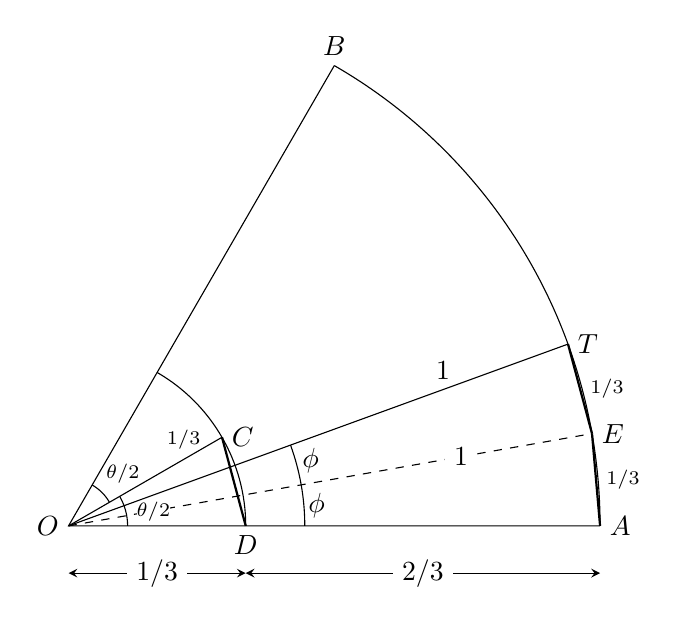
\begin{tikzpicture}[scale=.75]
\coordinate (O) at (0,0)
  node[left] {$O$}
  node[above right,xshift=10pt,yshift=12pt] {\sm{\theta/2}};

\coordinate (A) at (9cm,0);
\node[right] at (A) {$A$};
\coordinate (B) at (60:9);
\node[above] at (B) {$B$};
\draw (A) arc(0:60:9);
\draw (B) -- (O) -- (A);
\coordinate (D) at (3,0);
\node[below] at (D) {$D$};
\draw[name path=third] (D) arc(0:60:3);
\coordinate (C) at (30:3);
\node[right] at (C) {$C$};
\draw (O) -- node[above,near end] {\sm{1/3}} (C);
\draw[thick] (D) -- (C);
\coordinate (E) at (10:9);
\node[right] at (E) {$E$};
\draw[thick] (A) -- node[right] {\sm{1/3}} (E);
\coordinate (T) at (20:9);
\node[right] at (T) {$T$};
\draw[thick] (E) -- node[right] {\sm{1/3}} (T);
\draw (O) -- node[above,near end] {$1$} (T);

\draw (	1,0) arc (0:30:1);
\draw (30:.8) arc (30:60:.8);
\draw (4,0) arc (0:20:4);
\node at (4.2,0.35) {$\phi$}; 
\node at (4.1,1.1) {$\phi$}; 

\draw[dashed] (O) --
  node[fill=white,inner sep=0pt,very near start,
       xshift=7pt,yshift=1pt] {\sm{\theta/2}} 
  node[fill=white,near end] {$1$} (E);

\draw[<->] (3,-.8) -- node[fill=white] {$2/3$} +(6,0);
\draw[<->] (0,-.8) -- node[fill=white] {$1/3$} +(3,0);
\end{tikzpicture}
\end{center}
\caption{Second approximate trisection}
\label{f.trisect-second-approx}
\end{figure}

\begin{theorem}
\[
\cos\phi=1 - \frac{1}{9}(1-\cos(\theta/2))=1 - \frac{2}{9}\sin^2(\theta/4)\,.
\]
\end{theorem}

\begin{proof} By the Law of Cosines in $\triangle DOC$:
\[
\overline{CD}= \left(\frac{1}{3}\right)^2+\left(\frac{1}{3}\right)^2-2\left(\frac{1}{3}\right)\left(\frac{1}{3}\right)\cos (\theta/2)=\frac{2}{9}(1-\cos(\theta/2))\,.
\]

By the Law of Cosines in $\triangle EOA$:
\[
\overline{AE} = 1^2+1^2-2\cdot 1\cdot 1\cdot \cos \phi=2(1-\cos \phi)\,.
\]

\newpage

Equating the two expressions for $\overline{CD}=\overline{AE}$ and simplifying we get:
\[
\cos \phi = 1 - \frac{1}{9}(1-\cos(\theta/2))\,.
\]
Since $\cos 2\alpha= \cos^2 \alpha-\sin^2\alpha=1-2\sin^2\alpha$, and therefore $1-\cos 2\alpha=2\sin^2\alpha$, we have the alternate formula:
\[
\cos \phi = 1 - \frac{2}{9}\sin^2(\theta/4)\,.
\]
\end{proof}

This is an approximation to a trisection $2\phi=\theta/3$. For $\theta=60^\circ$:
\[
2\cos^{-1}\left(1 - \frac{1}{9}(1-\cos 30^\circ)\right)\approx 19.8^\circ\approx 20^\circ\,.
\]

Table~\ref{t.trisect-second-approx} shows the errors for a range of acute angles. This construction is much less accurate than the one in Sect.~\ref{sub.trisect-approx1}.

\begin{table}[t]
\caption{Errors in the second approximate trisection}\label{t.trisect-second-approx}
\[
%
\begin{array}{r@{\hspace{5mm}}r@{\hspace{5mm}}r@{\hspace{5mm}}r@{\hspace{5mm}}r}
\hline
\noalign{\smallskip}
\theta ({}^\circ) & \theta/3 ({}^\circ)& \cos^{-1} 2\phi ({}^\circ) & \mathrm{Error} ({}^\circ) & \mathrm{Error (\%)}\\
\noalign{\smallskip}\svhline\noalign{\smallskip}
  5 &    1.667 &    1.667  &     0.000 &    0.007 \\
 10 &    3.333 &    3.332  &     0.001 &    0.028 \\
 15 &    5.000 &    4.997  &     0.003 &    0.063 \\
 20 &    6.667 &    6.659  &     0.008 &    0.113 \\
 25 &    8.333 &    8.319  &     0.015 &    0.176 \\
 30 &   10.000 &    9.975  &     0.025 &    0.254 \\
 35 &   11.667 &   11.626  &     0.040 &    0.346 \\
 40 &   13.333 &   13.273  &     0.060 &    0.451 \\
 45 &   15.000 &   14.914  &     0.086 &    0.571 \\
 50 &   16.667 &   16.549  &     0.118 &    0.705 \\
 55 &   18.333 &   18.177  &     0.156 &    0.853 \\
 60 &   20.000 &   19.797  &     0.203 &    1.015 \\
 65 &   21.667 &   21.408  &     0.258 &    1.192 \\
 70 &   23.333 &   23.011  &     0.322 &    1.382 \\
 75 &   25.000 &   24.603  &     0.397 &    1.586 \\
 80 &   26.667 &   26.185  &     0.481 &    1.805 \\
 85 &   28.333 &   27.756  &     0.577 &    2.038 \\
 \noalign{\smallskip}
 \hline
 \end{array}
\]
\end{table}


%%%%%%%%%%%%%%%%%%%%%%%%%%%%%%%%%%%%%%%%%%%%%%%%%%%%%%%%%%%%

\newpage

\section{Trisection Using a Neusis}\label{s.neusis}\index{Trisection of an angle!neusis@with a neusis}
\index{Neusis!trisection of an angle}

The term \emph{straightedge} is used instead of \emph{ruler} because a straightedge has no marks on it. It can only be used to construct a straight line between two given points. Archimedes\index{Archimedes} showed that a \emph{neusis}, a straightedge with two marks that are a fixed distance apart, can be used to trisect an angle (Fig.~\ref{f.neusis}). We define the distance between the marks to be $1$.

\begin{figure}[b]
\begin{center}
\begin{tikzpicture}[scale=3.5]
\draw (-1,1.05) rectangle +(3.2,.1);
\draw[thick] (1.89,1.05) -- +(0,.1);
\draw[thick] (.73,1.05) -- +(0,.1);
\draw[<->] (.73,1.25) -- node[fill=white] {$1$} (1.89,1.25);
\end{tikzpicture}
\end{center}
\caption{A neusis}\label{f.neusis}
\end{figure}

\begin{figure}[t]
\begin{center}
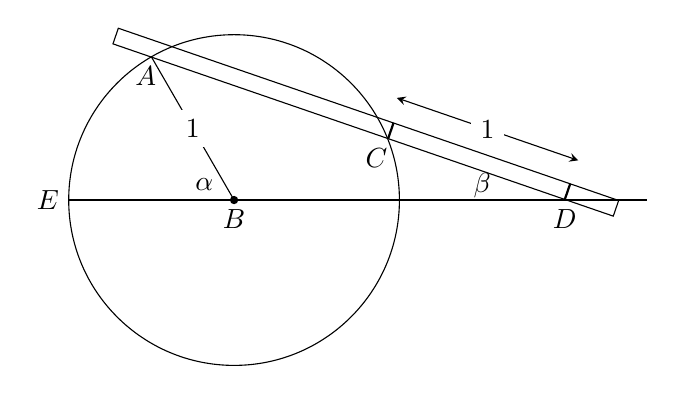
\begin{tikzpicture}[scale=2.1]
\coordinate (origin) at (0,0) node[below] {$B$} ;
\draw[name path=circle] (origin) circle [radius=1];
\draw (origin) node[above left,xshift=-4pt] {$\alpha$} -- node[fill=white] {$1$} (120:1) coordinate (a) node[below,xshift=-2pt] {$A$} ;
\draw (-1,0) -- (2.5,0);
\path[name path=ad] (a) -- (0,0 -| 2,0) coordinate (d) node[below] {$D$} ;
\path[name intersections={of=circle and ad,by={c,a1}}];
\coordinate (e) at (-1,0);
\vertex{origin};
\node [below,xshift=-4pt] at (c) {$C$};
\node [left] at (e) {$E$};
\node at (1.5,2.5pt) {$\beta$};
\begin{scope}[rotate=-19,yshift=-11.25pt]
\draw (-1,1.05) rectangle +(3.2,.1);
\draw[thick] (1.89,1.05) -- +(0,.1);
\draw[thick] (.76,1.05) -- +(0,.1);
\draw[<->] (.73,1.3) -- node[fill=white] {$1$} (1.89,1.3);
\end{scope}
\end{tikzpicture}
\end{center}
\caption{The neusis construction for trisecting an angle (1)}\label{f.trisect-neusis-1}
\end{figure}
\noindent\textbf{Construction:}
Let $\alpha=\angle ABE$ be an arbitrary angle in a unit circle with center $B$, where the radius of the circle equals the distance between the marks on the neusis. Extend the radius $\overline{EB}$ beyond the circle. Place an edge of the neusis on $A$ and move it until it intersects the extension of $\overline{EB}$ at $D$ and the circle at $C$, using the marks so that the length of the line segment $\overline{CD}$ is $1$.\footnote{This operation is called \emph{verging}.} Construct the line $\overline{AD}$. Denote $\angle CDB=\beta$ (Fig.~\ref{f.trisect-neusis-1}).

\begin{theorem} $\beta=\alpha/3$.
\end{theorem}
\begin{proof}
Construct $\overline{BC}$ and denote the angles and line segments as shown in Fig.~\ref{f.trisect-neusis-2}.
$\triangle ABC$ and $\triangle BCD$ are isoceles triangles: $\overline{AB} = \overline{BC}$ are radii of the same circle and $\overline{BC} = \overline{CD}$ by construction using the neusis. Since the sum of the angles of a triangle is equal to $180^\circ$ and the sum of supplementary angles is also equal to $180^\circ$, we have:
\begin{eqnarray*}
\epsilon &=& 180^\circ - 2\beta\\
\gamma &=& 180^\circ - \epsilon = 2\beta\\
\delta &=& 180^\circ - 2\gamma = 180^\circ - 4\beta\\
\alpha &=& 180^\circ - \delta - \beta=3\beta\,.
\end{eqnarray*}
\end{proof}

\begin{figure}[tbh]
\begin{center}
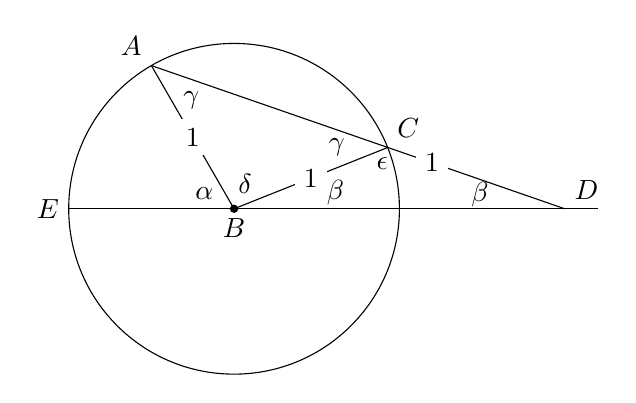
\begin{tikzpicture}[scale=2.1]
\coordinate (origin) at (0,0) node[below] {$B$} ;
\draw[name path=circle] (origin) circle [radius=1];
\draw (origin)
  node[above left,xshift=-4pt] {$\alpha$}
  node[above,xshift=4pt,yshift=2pt] {$\delta$}
  node[above right,xshift=30pt,yshift=-2pt] {$\beta$} --
  node[fill=white] {$1$} (120:1)
  coordinate (a) node[above left] {$A$};
\draw (-1,0) -- (2.2,0);
\draw[name path=ad] (a)
  node[below right,xshift=8pt,yshift=-6pt] {$\gamma$} -- 
  (0,0 -| 2,0) coordinate (d)
  node[left,xshift=-24pt,yshift=5pt] {$\beta$}
  node[above right] {$D$};
\path[name intersections={of=circle and ad,by={c,a1}}];
\draw (origin) -- node[fill=white] {$1$}(c) node[above right] {$C$} node[left,xshift=-12pt] {$\gamma$} node[below,xshift=-2pt,yshift=0pt] {$\epsilon$};
\coordinate (e) at (-1,0);
\vertex{origin};
\node [left] at (e) {$E$};
\path (c) -- node[fill=white,near start] {$1$} (d);
\end{tikzpicture}
\end{center}
\caption{The neusis construction for trisecting an angle (2)}\label{f.trisect-neusis-2}
\end{figure}

%%%%%%%%%%%%%%%%%%%%%%%%%%%%%%%%%%%%%%%%%%%%%%%%%%%%%%%%%%%%%

\newpage

\section{Doubling the Cube with a Neusis}\label{s.neusis-doubling}

Given a cube $C$ construct another cube with twice its volume. If the volume of $C$ is $V$ its sides are of length $\sqrt[3]{V}$. The sides of a cube with twice the volume are $\sqrt[3]{2 V}=\sqrt[3]{2}\cdot\sqrt[3]{V}$, so if we can construct $\sqrt[3]{2}$ we can double the cube.

\smallskip

\noindent\textbf{Construction:}
Construct the unit equilateral triangle $\triangle ABC$ and extend $\overline{CA}$ with another unit line segment to $D$. Construct rays extending $\overline{AB}$ and $\overline{DB}$. Place the neusis on point $C$ and move it until one mark on the neusis is placed on the ray $\overline{AB}$ at $P$ and the other mark is placed on the ray $\overline{DB}$ at $Q$. Denote $\overline{CQ}=x$ and $\overline{BP}=y$ (Fig.~\ref{f.double-neusis}).

\begin{figure}[b]
\begin{center}
\begin{tikzpicture}[scale=.7]
\clip (-.5,-.4) rectangle +(11,6.5);
\coordinate (D) at (0,0) node[left] {$D$};
\draw (D) -- ++(60:6) coordinate (C) node[above] {$C$};
\coordinate (A) at (60:3);
\node[left] at (A) {$A$};
\draw (A) -- ++(3,0) coordinate (B) -- (C);
\node[below right] at (B) {$B$};
\path[name path=DQ] (D) -- ($(D)!1.7!(B)$);
\path[name path=AP] (A) -- ($(A)!3!(B)$);
% 3*(1+\sqrt[3]{2}) = 6.78
\path[name path=CP] (C) circle (6.78cm);
\path[name intersections={of=CP and AP,by={P}}];
\draw[name path=CP] (C) -- (P);
\path[name intersections={of=CP and DQ,by={Q}}];
\node[above] at (Q) {$Q$};
\node[right] at (P) {$P$};
\draw (D) -- (Q);
\draw (B) -- (P);
\path (D) -- node[left] {$1$} (A) -- node[left] {$1$} (C) --
  node[right] {$1$} (B) -- node[below] {$1$} (A);
\path (C) -- node[above] {$x$} (Q) -- node[above] {$1$} (P) -- 
  node[below] {$y$} (B);
\end{tikzpicture}
\end{center}
\caption{Doubing the cube with a neusis}\label{f.double-neusis}
\end{figure}

\begin{theorem}\index{Doubling a cube!neusis@with a neusis}
\index{Neusis!doubling of a cube}
$x=\sqrt[3]{2}$.
\end{theorem}

\begin{proof}
Since $\triangle ABC$ is equilateral, $\cos \angle CAP=\cos 60^\circ=\frac{1}{2}$ and by the Law of Cosines\index{Law of cosines} in $\triangle APC$:
\begin{subeqnarray}
\overline{CP}^2&=&\overline{AC}^2+\overline{AP}^2-2\cdot \overline{AC}\cdot\overline{AP}\cos 60^\circ\\
(x+1)^2&=&1^2+(y+1)^2-2\cdot 1\cdot (y+1)\cdot \frac{1}{2}\\
x^2+2x&=&y^2+y\slabel{eq.eq-cube-double}\,.
\end{subeqnarray}

By Menelaus's theorem (Thm.~\ref{thm.menelaus}):
\[
\displaystyle\frac{\overline{AB}}{\overline{BP}}\cdot
\displaystyle\frac{\overline{PQ}}{\overline{QC}}\cdot
\displaystyle\frac{\overline{CD}}{\overline{DA}}=1\,.
\]

\newpage

Therefore:
\begin{subeqnarray}
\displaystyle\frac{1}{y}\cdot
\displaystyle\frac{1}{x}\cdot
\displaystyle\frac{2}{1}&=&1\\
xy&=&2\,.\slabel{eq.menelaus-xy2}
\end{subeqnarray}

Substituting Eq.~\ref{eq.menelaus-xy2} into Eq.~\ref{eq.eq-cube-double} gives:
\begin{eqnarray*}
x^2+2x&=&\frac{4}{x^2}+\frac{2}{x}\\
x^4+2x^3&=&4+2x\\
x^3(x+2)&=&2(x+2)\\
%x^3&=&2\\
x&=&\sqrt[3]{2}\,.
\end{eqnarray*}
\end{proof}


%%%%%%%%%%%%%%%%%%%%%%%%%%%%%%%%%%%%%%%%%%%%%%%%%%%%%%%%%%%%%
\section{Trisection Using a Quadratrix}\label{s.q}

\index{Trisection of an angle!quadratrix@with a quadratrix}

Let $\overline{ABCD}$ be a square. Let $l_1$ be a line segment placed initially at $\overline{DC}$ and let $l_2$ be a line segment placed initially at $\overline{AD}$. Move $l_1$ move at a constant linear velocity until it reaches $\overline{AB}$ and rotate $l_2$ at a constant angular velocity clockwise on $A$ until it also reaches $\overline{AB}$. Assume that they reach $\overline{AB}$ together. For example, if $l_2$ rotates at $1^\circ$/second and the side of the square is $9$ centimeters, $l_1$ must move at $0.1$ cm/second. The trace of their point of intersection $P$ is called a \emph{quadratrix curve}\index{Quadratrix} or simply a \emph{quadratrix} (Fig.~\ref{f.trisect-quad-curve}). Its definition is attributed to the mathematician Hippias\index{Hippias}.

\begin{figure}[b]
\subfigures
\leftfigure[c]{
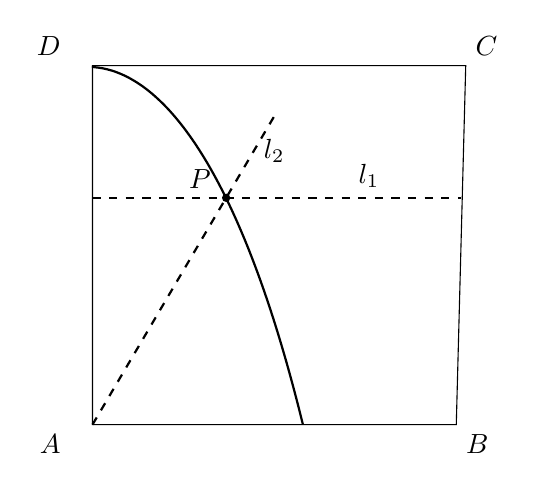
\begin{tikzpicture}[scale=.6,domain=.03:1.555,samples=100]
\draw (.1,.2)
  node[below left,xshift=-8pt] {$A$} -- 
  (7.8,.2) 
  node[below right] {$B$} -- 
  (8,7.8) 
  node[above right] {$C$} -- 
  (.1,7.8) node[above left,xshift=-8pt] {$D$} -- 
  cycle;
\draw[thick,dashed,name path=arm] (.1,.2) -- node[right,very near end] {$l_2$} (59.6:7.9);
\draw[thick,dashed,name path=horiz] (.1,5) -- node[above,near end] {$l_1$} +(7.8,0);
\path[name intersections={of=arm and horiz,by={A}}];
\node[above left,xshift=-2pt] at (A) {$P$};
\vertex{A};
\draw[thick] plot (4.6*.637*\x,{12.2*.637*\x*cot(\x r)});
\end{tikzpicture}
}
\hfill
\rightfigure[c]{
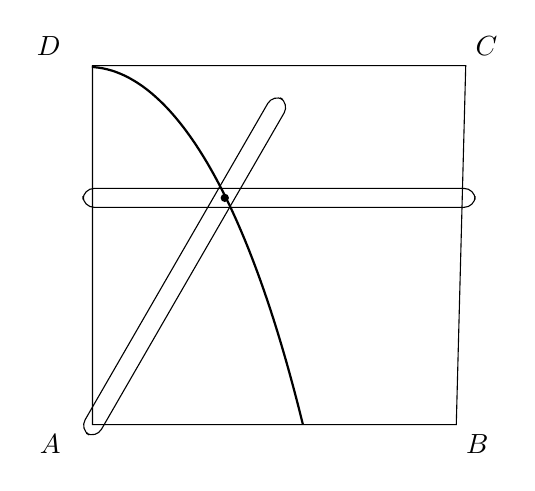
\begin{tikzpicture}[scale=.6,domain=.03:1.555,samples=100]
\draw (.1,.2) node[below left,xshift=-8pt] {$A$} -- (7.8,.2) node[below right] {$B$} -- (8,7.8) node[above right] {$C$} -- (.1,7.8) node[above left,xshift=-8pt] {$D$} -- cycle;
\draw[rounded corners,rotate=60] (0,-.2) rectangle (8.2,.2);
\draw[rounded corners] (-.1,4.8) rectangle (8.2,5.2);
\fill (2.9,5) circle [radius=2.5pt];
\draw[thick] plot (4.6*.637*\x,{12.2*.637*\x*cot(\x r)});
\end{tikzpicture}
}
\leftcaption{A quadratrix curve}\label{f.trisect-quad-curve}
\rightcaption{A quadratrix compass}\label{f.trisect-quad-compass}
\end{figure}

A quadratrix can be constructed using a \emph{quadratrix compass}\index{Quadratrix!compass} as shown in Fig.~\ref{f.trisect-quad-compass}. It consists of two (unmarked) straightedges that move as described above. A joint constrains them to move together and traces out the curve.


\begin{figure}[b]
\begin{center}
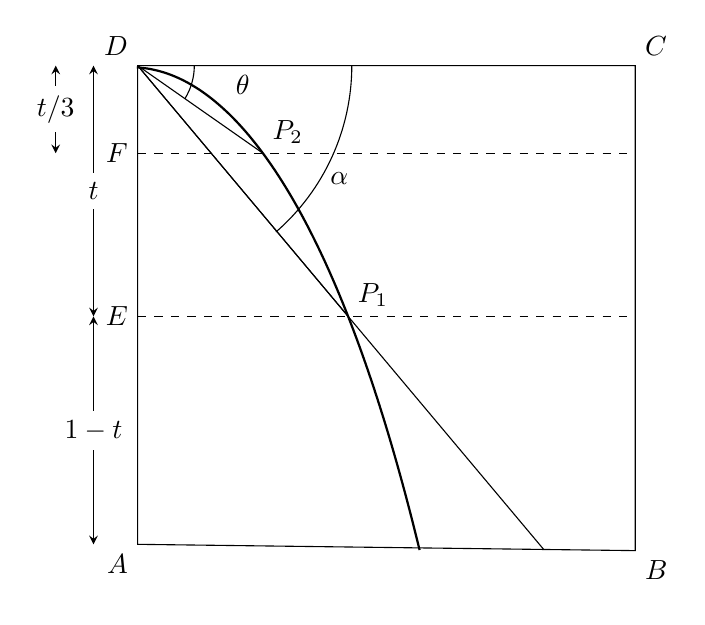
\begin{tikzpicture}[scale=.8,domain=.03:1.562,samples=100]
\draw (.1,7.8) coordinate (start)
  node[above left] {$D$}
  node[below right,xshift=32pt] {$\theta$} -- 
  (.1,.2) node[below left] {$A$} -- 
  (8,.1)  node[below right] {$B$} -- 
  (8,7.8) node[above right] {$C$} -- 
  cycle;
\draw[name path=curve,thick] plot (4.6*.637*\x,{12.2*.637*\x*cot(\x r)});
% To ensure intersection at node D, path should extend to the upper left of D
\coordinate (twenty-a) at ($(start)+(-35:9)$);
\path[name path=twenty] ($(start)!-.1!(twenty-a)$) -- (twenty-a);
\path[name path=sixty] (start) -- +(-50:11);
\path[name path=xaxis] (.1,.2) -- (8,.1);
\path[name intersections={of=twenty and curve,by={x1,tri}}];
\draw (start) -- (tri);
\node[above right] at (tri) {$P_2$};
\path[name intersections={of=sixty and curve,by={x2,angle}}];
\node[above right] at (angle) {$P_1$};
\draw (start) -- (angle);
\path[name intersections={of=xaxis and curve,by=x}];
\path[name intersections={of=sixty and xaxis,by=sixty-x}];
\draw (start) -- (sixty-x);

\path (tri) -- (tri -| .1,.2) coordinate (t3);
\draw[dashed] (t3) -- +(7.9,0);
\node[left] at (t3) {$F$};
\path (angle) -- (angle -| .1,.2) coordinate (t);
\draw[dashed] (t) -- +(7.9,0);
\node[left] at (t) {$E$};
\draw[<->] (-1.2,7.8) -- node[fill=white] {$t/3$} (-1.2,7.8 |- t3);
\draw[<->] (-.6,7.8) -- node[fill=white] {$t$} (-.6,7.8 |- t);
\draw[<->] (-.6,7.8 |- t) -- node[fill=white] {$1-t$} (-.6,.2);
\draw (3.5,7.8) arc[start angle=0,delta angle=-49,radius=3.5];
\draw (1,7.8) arc[start angle=0,delta angle=-32,radius=1];
\node at (3.3,6) {$\alpha$}; 
\end{tikzpicture}
\end{center}
\caption{Trisection of an angle using a quadratrix}\label{f.trisect-quad-trisect}
\end{figure}

A quadratrix can be used to trisect an angle.

\noindent\textbf{Construction:}
Let $\angle CDP_1=\alpha$ be an arbitrary angle, where $P_1$ is the intersection of the line defining the angle $\alpha$ relative to $\overline{DC}$ and the quadratrix. Construct a line through $P_1$ parallel to $\overline{DC}$ and denote its intersection with $\overline{AD}$ by $E$. Denote the line segment $\overline{DE}$ by $t$ and trisect it (Sect.~\ref{s.trisect-constructible}) to obtain point $F$ that is $t/3$ from $\overline{DC}$. Let $P_2$ be the intersection of a line from $F$ parallel to $\overline{DC}$ and the quadratrix, and denote by $\theta$ the angle between $\overline{DC}$ and $\overline{DP_2}$ (Fig.~\ref{f.trisect-quad-trisect}).

\begin{theorem}
$\theta = \alpha/3$.
\end{theorem}
\begin{proof}
$E$ has $y$-coordinate $1-t$ so by construction $F$ has $y$-coordinate $1-(t/3)$. Since the constant linear velocity of the horizontal line is proportional to the constant angular velocity of the rotating line $\theta/\alpha = (t/3)/t$ and $\theta = \alpha/3$.
\end{proof}

\newpage

\section{Constructible Numbers}\label{s.trisect-constructible}
\index{Constructible number}

Let $l$ be a line segment defined to be of length $1$.

\begin{definition}
A number $a$ is \emph{constructible} if and only if a line segment of length $a$ can be constructed with a straightedge and compass starting from $l$.
\end{definition}

Given line segment $l=\overline{AB}$, construct a line containing $\overline{AB}$ and use the compass to find a point $C$ on the line that is a distance of $1$ from $B$. Then $\overline{AC}$ is of length $2$ so the number $2$ is constructible. A line segment $\overline{BD}$ of length $1$ can be constructed perpendicular to $\overline{AB}$ at $B$. The hypotenuse of the triangle $\triangle ABD$ is of length $\sqrt{2}$ so the number $\sqrt{2}$ is constructible.

\begin{theorem}\label{thm.trisect-constructible}
A number is \emph{constructible} if and only if it is the value of an expression built from the integers, the four arithmetic operations $\{+,-,\times,/\}$ and the operation of taking a square root $\surd$.
\end{theorem}

\begin{proof} First we show that the values of these expressions are constructible.
\index{Constructible number!arithmetic operation}

\medskip

\begin{figure}[b]
\begin{center}
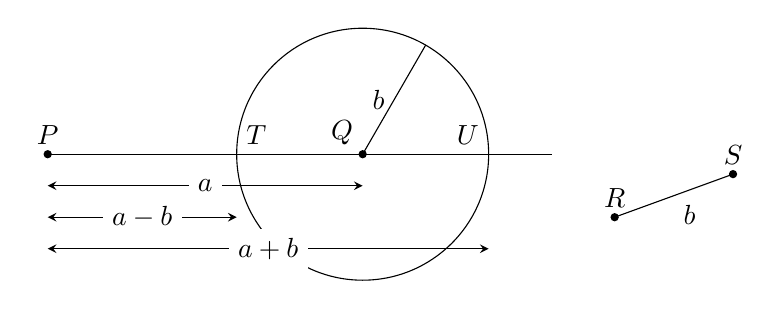
\begin{tikzpicture}[scale=.8]
\coordinate (P) at (0,0);
\coordinate (Q) at (5,0);
\coordinate (T) at (3,0);
\coordinate (U) at (7,0);
\vertex{P};
\vertex{Q};
\draw (P) -- (Q);
\node[above] at (P) {$P$};
\node[above left] at (Q) {$Q$};
\node[above left] at (U) {$U$};
\node[above right] at (T) {$T$};
\draw (5,0) -- (8,0);
\draw (5,0) circle[radius=2cm];
\draw (5,0) -- node[left] {$b$} ++(60:2cm);
\coordinate (R) at (9,-1);
\coordinate (S) at ($(9,-1) + (20:2cm)$);
\vertex{R};
\vertex{S};
\draw (R) node[above] {$R$} --
  node[below right] {$b$} (S)
  node[above] {$S$};
\draw[<->] (0,-.5) -- node[fill=white] {$a$} (5,-.5);
\draw[<->] (0,-1) -- node[fill=white] {$a-b$} (3,-1);
\draw[<->] (0,-1.5) -- node[fill=white] {$a+b$} (7,-1.5);
\end{tikzpicture}
\end{center}
\caption{Construction of addition and subtraction}\label{f.trisect-add-subtract}
\end{figure}

\noindent\textbf{Addition and subtraction:}
Given line segments $\overline{PQ}=a$ and $\overline{RS}=b$, construct a circle centered at $Q$ with radius $b$ (Fig.~\ref{f.trisect-add-subtract}). Extend $\overline{PQ}$ until it intersects the circle at $U$. Then $\overline{PTQU}$ is a line segment, where $\overline{PT}=a-b$ and $\overline{PU}=a+b$.

\newpage

\noindent\textbf{Multiplication:}
By similar triangles in Fig.~\ref{f.trisect-multiplication},
$(1/b)=(a/\overline{OA})$, so $\overline{OA}=ab$.

\medskip

\noindent\textbf{Division:}
By similar triangles in Fig.~\ref{f.trisect-division},
$(1/b)=(\overline{OD}/a)$, so $\overline{OD}=(a/b)$.

\begin{figure}[t]
\subfigures
\leftfigure[c]{
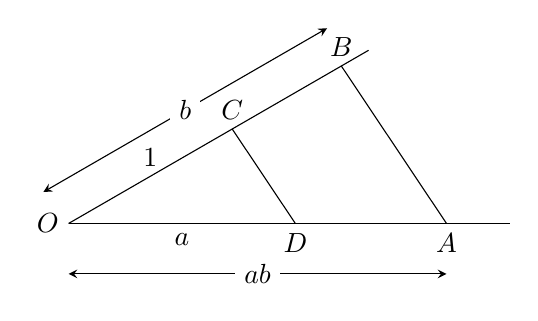
\begin{tikzpicture}[scale=.8]
\draw[name path=horz] (0,0) coordinate (o) -- (7,0);
\node[left] at (o) {$O$};
\coordinate (a) at (6,0);
\node[below]  at (a) {$A$};
\draw (o) -- (30:5.5);
\coordinate (c) at (30:3);
\coordinate (b) at (30:5);
\node[above] at (c) {$C$};
\node[above] at (b) {$B$};
\draw (a) -- (b);
\path[name path=par] (c) -- +($(a)-(b)$);
\path[name intersections={of=par and horz,by=d}];
\node[below] at (d) {$D$};
\draw (c) -- (d);
\draw[<->] (-.4,.5) -- node[fill=white] {$b$} +(30:5.2);
\path (o) -- node[above] {$1$} (c);
\draw[<->] (0,-.8) -- node[fill=white] {$ab$} +(6,0);
\path (o) -- node[below] {$a$} (d);
\end{tikzpicture}
}
\hfill
\rightfigure[c]{
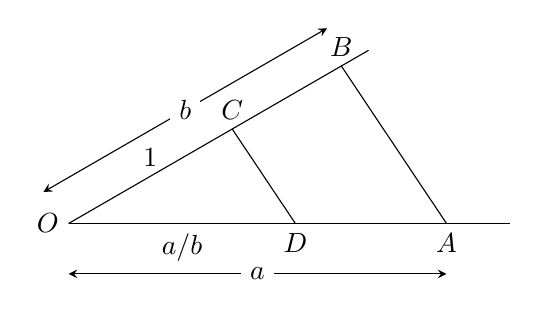
\begin{tikzpicture}[scale=.8]
\draw[name path=horz] (0,0) coordinate (o) -- (7,0);
\node[left] at (o) {$O$};
\coordinate (a) at (6,0);
\node[below]  at (a) {$A$};
\draw (o) -- (30:5.5);
\coordinate (c) at (30:3);
\coordinate (b) at (30:5);
\node[above] at (c) {$C$};
\node[above] at (b) {$B$};
\draw (a) -- (b);
\path[name path=par] (c) -- +($(a)-(b)$);
\path[name intersections={of=par and horz,by=d}];
\node[below] at (d) {$D$};
\draw (c) -- (d);
\draw[<->] (-.4,.5) -- node[fill=white] {$b$} +(30:5.2);
\path (o) -- node[above] {$1$} (c);
\draw[<->] (0,-.8) -- node[fill=white] {$a$} +(6,0);
\path (o) -- node[below] {$a/b$} (d);
\end{tikzpicture}
}
\leftcaption{Construction of multiplication}\label{f.trisect-multiplication}
\rightcaption{Construction of division}\label{f.trisect-division}
\end{figure}

\medskip

\noindent\textbf{Square roots:}
\index{Constructible number!square root}
Given a line segment $\overline{BC}=a$, construct $\overline{AB} =1+a$ and a semicircle with $\overline{AB}$ as its diameter. Construct a perpendicular at $C$ and let $D$ be the intersection of the perpendicular and the circle (Fig.~\ref{f.trisect-square-root}). $\angle ADB$ is a right angle because it is subtended by a diameter. By similar triangles $(h/1)=(a/h)$, so $h^2=a$ and $h=\sqrt{a}$.

\begin{figure}[b]
\begin{center}
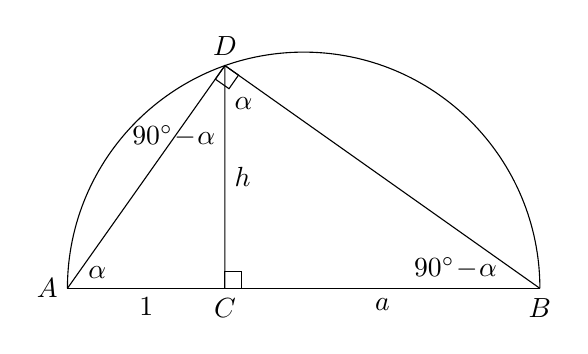
\begin{tikzpicture}[scale=1]
\draw[name path=horz] (0,0) coordinate (a) -- (6,0);
\node[left] at (a) {$A$};
\coordinate (b) at (6,0);
\node[below] at (b) {$B$};
\draw[name path=circle] (b) arc(0:180:3);
\path[name path=perp] (2,0) -- +(0,3.2);
\coordinate (c) at (2,0);
\node[below] at (c) {$C$};
\path[name intersections={of=circle and perp,by=d}];
\node[above] at (d) {$D$};
\draw (c) -- node[right] {$h$} (d);
\path (a) -- node[below] {$1$} (c) -- node[below] {$a$} (b);
\draw (c) rectangle +(6pt,6pt);
\draw (a) -- (d) -- (b);
\draw[rotate=-125] (d) rectangle +(6pt,6pt);
\node[above right,xshift=4pt] at (a) {$\alpha$};
\node[above left,xshift=-12pt] at (b) {$90^\circ\!-\!\alpha$};
\node[below right,yshift=-8pt] at (d) {$\alpha$};
\node[below left,xshift=0pt,yshift=-18pt] at (d) {$90^\circ\!-\!\alpha$};
\end{tikzpicture}
\end{center}
\caption{Construction of a square root}
\label{f.trisect-square-root}
\end{figure}

\medskip

To prove the converse of the theorem, we need to determine what expressions can be constructed by a straightedge and compass. There are three constructions:\footnote{For clarity these are illustrated for specific values rather than the most general equations.}

\begin{enumerate}
\item Two lines intersect in a point (Fig.~\ref{f.constructible-two-lines}). The coordinates of the intersection can be derived from the equations of the two lines
$y=x$ and $y=4x-2$. The point of intersection is $P= (2/3, 2/3)$.

\item A line intersects a circle in zero, one or two points (Fig.~\ref{f.constructible-line-circle}). The coordinates of the intersections can be derived from the equations of the line $y=x$ and the circle $x^2+y^2=4$. The points of intersection are
$P=(\sqrt{2}, \sqrt{2})$ and $Q=(-\sqrt{2}, -\sqrt{2})$.

\item Two circles intersect in zero, one or two points (Fig.~\ref{f.constructible-two-circles}). The coordinates of the intersections can be derived from the equations of the two circles $(x-1)^2+y^2=4$, $(x+1)^2+y^2=4$. The points of intersection are $P=(0,\sqrt{2}),Q=(0,-\sqrt{2})$.
\end{enumerate}
\end{proof}

\begin{figure}[t]
\subfigures
\leftfigure[c]{
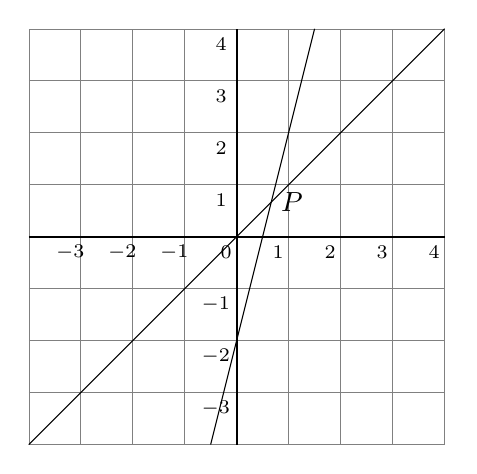
\begin{tikzpicture}[scale=.66]
\draw[step=10mm,white!50!black,very thin] (-4,-4) grid (4,4);
\draw[thick] (-4,0) -- (4,0);
\draw[thick] (0,-4) -- (0,4);
\coordinate (O) at (0,0);
\foreach \x in {-3,...,4}
  \node at (\x-.2,-.3) {\sm{\x}};
\foreach \y in {-3,...,-1}
  \node at (-.4,\y-.3) {\sm{\y}};
\foreach \y in {1,...,4}
  \node at (-.3,\y-.3) {\sm{\y}};
\draw[name path=eq1] (-4,-4) -- (4,4);
\draw[name path=eq2] (-.5,-4) -- (1.5,4);
\path[name intersections={of=eq1 and eq2,by={P}}];
\node[right] at (P) {$P$};
\end{tikzpicture}
}
\hfill
\rightfigure[c]{
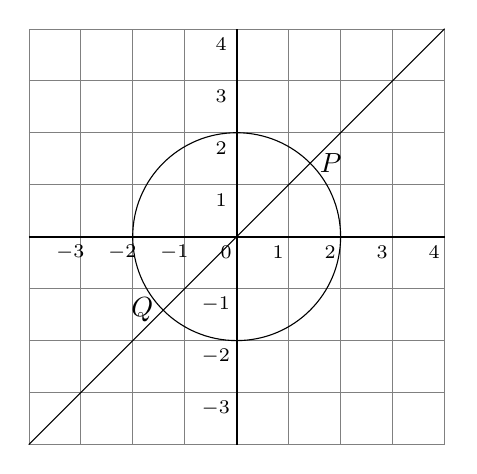
\begin{tikzpicture}[scale=.66]
\coordinate (O) at (0,0);
\draw[step=10mm,white!50!black,very thin] (-4,-4) grid (4,4);
\draw[thick] (-4,0) -- (4,0);
\draw[thick] (0,-4) -- (0,4);
\foreach \x in {-3,...,4}
  \node at (\x-.2,-.3) {\sm{\x}};
\foreach \y in {-3,...,-1}
  \node at (-.4,\y-.3) {\sm{\y}};
\foreach \y in {1,...,4}
  \node at (-.3,\y-.3) {\sm{\y}};
\coordinate (A) at (2,0);
\node[draw,circle through=(A),name path=circle] at (0,0) {};
\draw[name path=eq1] (-4,-4) -- (4,4);
\path[name intersections={of=eq1 and circle,by={P,Q}}];
\node[right] at (P) {$P$};
\node[left] at (Q) {$Q$};
\end{tikzpicture}
}
\leftcaption{The point of intersection of two lines}\label{f.constructible-two-lines}
\rightcaption{The points of intersection of a line and a circle}\label{f.constructible-line-circle}
\end{figure}


\begin{figure}[b]
\begin{center}
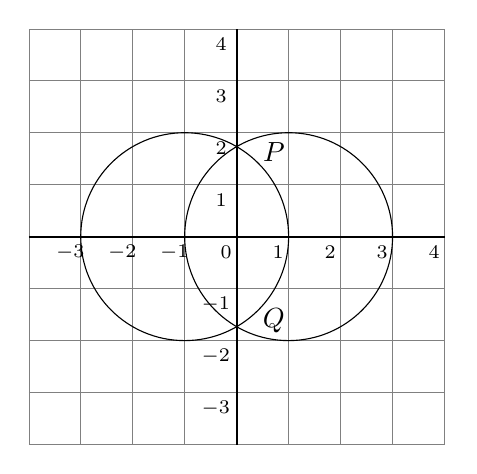
\begin{tikzpicture}[scale=.66]
\coordinate (O) at (0,0);
\draw[step=10mm,white!50!black,very thin] (-4,-4) grid (4,4);
\draw[thick] (-4,0) -- (4,0);
\draw[thick] (0,-4) -- (0,4);
\foreach \x in {-3,...,4}
  \node at (\x-.2,-.3) {\sm{\x}};
\foreach \y in {-3,...,-1}
  \node at (-.4,\y-.3) {\sm{\y}};
\foreach \y in {1,...,4}
  \node at (-.3,\y-.3) {\sm{\y}};
\coordinate (A) at (3,0);
\node[draw,circle through=(A),name path=circle1] at (1,0) {};
\coordinate (B) at (-3,0);
\node[draw,circle through=(B),name path=circle2] at (-1,0) {};
\path[name intersections={of=circle1 and circle2,by={P,Q}}];
\node[right,xshift=6pt,yshift=-2pt] at (P) {$P$};
\node[right,xshift=6pt,yshift=2pt] at (Q) {$Q$};
\end{tikzpicture}
\caption{The points of intersection of two circles}\label{f.constructible-two-circles}
\end{center}
\end{figure}

\newpage

\section{Constructible Numbers As Roots of Polynomials}\label{s.trisect-poly}
To show that a number is not constructible, we need to prove that it cannot be expressed using just integers and the operations $\{+,-,\times,/,\surd\}$.

We will show that constructible numbers are the roots of a certain class of polynomials and then prove that trisecting an angle and doubling a cube require the construction of roots of polynomials that are not in this class. Today these results are proved using field theory from abstract algebra, but here I give a proof that uses elementary mathematics. The proof is based on the following definition.

\begin{definition}
The \emph{depth} of an expression built from the integers and the operators $\{+,-,\times,/,\surd\}$ is the maximum level of nesting of square roots.
\end{definition}\index{Constructible number!depth of square roots}

\begin{example}
Consider the following expression:
\[
\sqrt{17+3\sqrt{17} - \sqrt{34-2\sqrt{17}}
  -2\sqrt{34+2\sqrt{17}} }\,.
\]
The depth is $3$ because at the right of the expression we have $\sqrt{17}$ which is nested within $\sqrt{34+2\sqrt{17}}$, which in turn is nested within $\sqrt{17+\cdots-\cdots-2\sqrt{34+2\sqrt{17}}}$.
\end{example}

\begin{theorem}
A expression of depth $n$ can be expressed as $a+b\sqrt{c}$ where $a,b,c$ are expressions of depth at most $n-1$.
\end{theorem}
\begin{proof}
Simple computations show that the expressions $(a_1+b_1\sqrt{c})\,\mathit{op}\,(a_2+b_2\sqrt{c})$ for the operators $\mathit{op}=\{+,-,\times\}$ result in expressions $a+b\sqrt{c}$ of depth $n-1$. For division the computation is a bit more complicated:
\begin{eqnarray*}
\frac{a_1+b_1\sqrt{c}}{a_2+b_2\sqrt{c}}&=&
\frac{(a_1+b_1\sqrt{c})(a_2-b_2\sqrt{c_2})}{(a_2+b_2\sqrt{c})(a_2-b_2\sqrt{c})}\\
&=&\frac{a_1a_2-b_1b_2c}{a_2^2-b_2^2c}+\frac{a_2b_1-a_1b_2}{a_2^2-b_2^2c}\sqrt{c}\,,
\end{eqnarray*}
which is of the form $a+b\sqrt{c}$ where $a,b,c$ are of depth $n-1$.
Finally, the square root of an expression of depth $n-1$ is an expression of depth $n$.
\end{proof}


\begin{theorem}\label{thm.trisect.conjugate}
Let $p(x)$ be a monic\index{Monic polynomial} cubic polynomial with rational coefficients:
\[
p(x)=x^3+a_2x^2+a_1x+a_0\,,
\]
and let $r=a+b\sqrt{c}$ be a root of $p(x)$ \emph{of minimal depth} $n$, where $a,b,c$ are of depth (at most) $n-1$. Then $r'=a-b\sqrt{c}$ is a root of $p(x)$ and $r\neq r'$.
\end{theorem}\index{Roots!cubic@of cubic polynomials|(}

\newpage

\begin{proof} Let us compute $p(r)$ which is equal to $0$ since $r$ is a root:
\[
\renewcommand{\arraystretch}{1.4}
\begin{array}{lcr}
(a+b\sqrt{c})^3+a_2(a+b\sqrt{c})^2+a_1(a+b\sqrt{c})+a_0&=\\
(a^3+3a^2b\sqrt{c}+3ab^2c+b^3c\sqrt{c})\\
\quad+\,a_2(a^2+2ab\sqrt{c}+b^2c) +a_1(a+b\sqrt{c}) +a_0&=\\
(a^3+3ab^2c+a_2a^2+a_2b^2c+a_1a+a_0)\\
\quad+\,(3a^2b+b^3c+2a_2ab+a_1b)\sqrt{c}&=\\
d+e\sqrt{c}&=&0\,.
\end{array}
\]
where $d,e$ are expressions of depth $n-1$ formed from the rational coefficients and $a,b,c$. Then $\sqrt{c}=-d/e$, so $a+b\sqrt{c}$ can be expressed as an expression of depth $n-1$, contracting the assumption that $a+b\sqrt{c}$ is of minimal depth $n$. Since $\sqrt{c}\neq 0$ and is of depth $n$, for $d+e\sqrt{c}$ to be zero it must be that $d=e=0$.

Consider now $r'=a-b\sqrt{c}$. By examining the above computation we see that $p(r')=d-e\sqrt{c}=0+0\cdot\sqrt{c}=0$, so $r'$ is also a root of $p$.

If $r= r'$ then $0=r-r'=2b\sqrt{c}$, which is true only if $b=0$ so $r,r'$ would be of depth $n-1$, again contradicting the assumption.
\end{proof}                                

\begin{theorem}
If a monic\index{Monic polynomial} cubic polynomial with rational coefficients:
\[p(x)=x^3+a_2x^2+a_1x+a_0\] has no rational roots then none of its roots is constructible.
\end{theorem}

\begin{proof} By the Fundamental Theorem of Algebra\index{Fundamental theorem of algebra}  (Thm.~\ref{thm.fundamental}) $p(x)$ has three roots $r_1,r_2,r_3$. Let $r_1=a+b\sqrt{c}$ be a root of minimal depth $n$. By the assumption that there are no rational roots, $n\geq 1$, and therefore $b\neq 0$ and $c\neq 0$. By Thm.~\ref{thm.trisect.conjugate}, $r_2=a-b\sqrt{c}$ is also a root. Perform the following multiplication:
\begin{subeqnarray}
(x-r_1)(x-r_2)(x-r_3)&=&x^3 -(r_1+r_2+r_3)x^2\\
&&\quad\; +\, (r_1r_2+r_1r_3+r_2r_3)x + r_1r_2r_3\slabel{eq.viete3}\\
a_2&=&-(r_1+r_2+r_3)\\
r_3&=&-(a_2+r_1+r_2)\,.
\end{subeqnarray}
Since $a_2$ is rational so is:
\[r_3=-a_2-(r_1+r_2)=-a_2-2a\,,\]
contradicting the assumption.
\end{proof}
\index{Roots!cubic@of cubic polynomials|)}

\section{Impossibility of the Classical Constructions}\label{s.trisect-impossible}

\begin{theorem}\label{thm.trisect.cube-root-irrational}
$\sqrt[3]{2}$ is irrational.
\end{theorem}
\begin{proof}
Assume that $\sqrt[3]{2}$ is rational and equal to $p/q$ where $p,q$ are integers with no common factors other than $\pm 1$. Then:
\begin{eqnarray*}
(p/q)^3&=&(\sqrt[3]{2})^3\\
p^3&=&2q^3\,,
\end{eqnarray*}
so $p$ must be divisible by $2$, say $p=2r$. Now:
\begin{eqnarray*}
8r^3&=&2q^3\\
q^3&=&4r^3\,,
\end{eqnarray*}
so $q$ is divisible by $2$, contradicting the assumption that $p,q$ have no common factor.
\end{proof}

\begin{theorem}
$x^3-2$ has no rational roots so it is impossible to double a cube with a straightedge and compass.\index{Doubling a cube!impossibility of}
\end{theorem}
\begin{proof} One of its roots is $\sqrt[3]{2}$ which by Thm.~\ref{thm.trisect.cube-root-irrational} is irrational. The other roots are the roots of the quadratic equation $x^2+\sqrt[3]{2}x+(\sqrt[3]{2})^2$ obtained by dividing $x^3-2$ by $x-\sqrt[3]{2}$. It is easy to check that its roots are not rational (in fact, not even real).
\end{proof}


\begin{theorem}
It is impossible to trisect an arbitrary angle with a straightedge and compass.
\end{theorem}
\begin{proof}
It is sufficient to show the impossibility for one angle. Let us try to trisect $60^\circ$ to obtain $20^\circ$.
\index{Trisection of an angle!impossibility of}
By Thm.~\ref{thm.triple-angle}:
\begin{eqnarray*}
\cos 3\alpha&=&4\cos^3\alpha -3\cos\alpha\\
\cos 60^\circ&=&4\cos^3 20^\circ -3\cos 20^\circ\,.
\end{eqnarray*}
Denote $x=\cos 20^\circ$ and $2x$ by $y$. Since $\cos 60^\circ=1/2$ we have:
\begin{eqnarray*}
4x^3 -3x-\frac{1}{2} &=& 0\\
8x^3-6x-1&=&0\\
y^3-3y-1&=&0\,.
\end{eqnarray*}

To prove that the polynomial $y^3-3y-1$ has no rational roots suppose that $y=a/b$ is a rational root with $a,b$ having no common factor other than $\pm 1$. Then:
\begin{subeqnarray}
(a/b)^3-3(a/b)-1&=&0\\
a^3-3ab^2&=&b^3\\
a(a-3b^2)&=&b^3\slabel{eq.trisect1}\\
a^3&=&b(b^2+3ab)\slabel{eq.trisect2}\,.
\end{subeqnarray}
By Eq.~\ref{eq.trisect1}, $b$ must be divisible by $a$, and by Eq.~\ref{eq.trisect2}, $a$ must be divisible by $b$, which is possible only if $a=b=\pm 1$ and $a/b=\pm 1$. By computation, $y=a/b=1$ and $y=a/b=-1$ are not roots of the polynomial.
\end{proof}


An alternate way of proving the impossibility of the constructions is to use the following theorem which we present without proof.

\begin{theorem}\label{thm.factor}
If a monic\index{Monic polynomial} polynomial $p(x)=x^n+a_{n-1}x^{n-1}+\cdots+a_0$ with integer coefficients has rational roots then it has integer roots.
\end{theorem}

To show the impossibility of duplicating a cube we need to show that:
\[
x^3-2=(x-r_2)(x-r_1)(x-r_0)
\]
has no integer roots. Since $r_0r_1r_2=-2$, all roots must divide $2$, so the only possible integer roots are $\pm 1, \pm 2$. A quick computation shows that none of them are roots.

To show the impossibility of trisecting an angle we need to show that $y^3-3y-1$ has no integer roots. An integer root must divide $-1$ but neither $1$ nor $-1$ are roots.

\subsection*{What Is the Surprise?}

Underwood Dudley has made an extensive study of what he calls ``cranks'' who waste years of their lives trying to trisect angles with a straightedge and compass. Not only do they delude themselves into thinking that this is possible, but, even worse, they think that a solution would be important. Of course, a solution would have no practical use, since tools such as the neusis and quadratrix can solve the problem exactly. The sheer number of such constructions is surprising, especially since many of them are clever and achieve good approximations. Computing the formulas associated with the constructions is an excellent exercise in trigonometry.

It is also surprising that proofs of the impossibility of these geometric constructions are purely algebraic using properties of roots of polynomials.

\subsection*{Sources}

Wikipedia \cite{wiki:tri, wiki:neu, wiki:quad} is a good source for the constructions in this chapter.
The two approximate trisections are from \cite[pp.
~67--68, 95--96]{dudley-budget}. The second example is attributed to the famous philosopher Thomas Hobbes. Both \cite[pp.~48--49]{martin} and \cite[pp.~6--7]{dudley-budget} discuss trisection using the quadratrix.
The doubling of the cube using a neusis is taken from \cite{dorrie2}.

A rigorous treatment of constructibility can be found in textbooks on abstract algebra such as \cite{fraleigh}, which contains a general proof of the converse of Thm~\ref{thm.trisect-constructible} in Sect.~32.
Theorem~\ref{thm.factor} is Thm.~23.11 of \cite{fraleigh}.
A relatively accessible presentation of Wantzel's proof can be found in \cite{suzuki}. My presentation of constructibility is based upon the presentations in \cite[Chap.~III]{courant} and \cite{laugwitz}.


\tikzsetfigurename{square}
% !TeX root = surprises.tex

\chapter{Squaring the Circle}\label{c.square}

%%%%%%%%%%%%%%%%%%%%%%%%%%%%%%%%%%%%%%%%%%%%%%%%%%%%%%%%%%%%%%%

\abstract*{Squaring the circle---the construction of a square with the same area as a given circle---is one of the three famous problems that the Greeks posed but were unable to solve. Unlike trisecting the angle and doubling the cube, where the impossibility follows from the properties of roots of polynomials, the impossibility of squaring the circle follows from the transcendentality of $\pi$, meaning that $\pi$ is not the root of any polynomial with rational coefficients. This is a difficult theorem that was finally proved in 1882. 
In this chapter we present three approximate constructions of the value of $\pi$, one by Adam Kocha\'{n}ski and two by Ramanujan. The chapter also shows that squaring the circle is possible using the quadratrix.}

%%%%%%%%%%%%%%%%%%%%%%%%%%%%%%%%%%%%%%%%%%%%%%%%%%%%%%%%%%%%%%%

Squaring the circle, the construction of a square with the same area as a given circle, is one of the three construction problems that the Greeks posed but were unable to solve. Unlike trisecting the angle and doubling the cube, where the impossibility follows from properties of the roots of polynomials, the impossibility of squaring the circle follows from the transcendentality of $\pi$: it is not the root of any polynomial with rational coefficients. This is a difficult theorem that was proved in 1882 by Carl von Lindemann\index{Lindemann, Carl von}.

Approximations to $\pi\approx 3.14159265359$ have been known since ancient times. Some simple but reasonably accurate approximations are:
\[
\displaystyle\frac{22}{7}\approx 3.142857,\quad \displaystyle\frac{333}{106}\approx 3.141509,\quad \displaystyle\frac{355}{113}\approx 3.141593\,.
\]

We present three constructions by a straightedge and compass of  approximations to $\pi$. One is by by Adam Kocha\'{n}ski (Sect.~\ref{s.square-kochanski}) and two are by Ramanujan (Sects.~\ref{s.square-ramanujan-first}, \ref{s.square-ramanujan-second}). Section~\ref{s.square-quad} how to square the circle using the quadratrix.

\enlargethispage{\baselineskip}

The following table shows the formulas for the lengths that are constructed, their approximate values, the difference between these values and the value of $\pi$ and the error in meters that results if the approximation is used to compute the circumference of the earth given that its radius is $6378$ km.
\[
\begin{array}{l@{\hspace{5mm}}c@{\hspace{5mm}}c@{\hspace{5mm}}c@{\hspace{5mm}}r}
\hline\noalign{\smallskip}
\textrm{Construction} & \textrm{Formula} &\textrm{Value} & \textrm{Difference} & \textrm{Error (m)}\\\svhline\noalign{\medskip}
\pi & -& 3.14159265359 & - & -\\\noalign{\medskip}
\textrm{Kocha\'{n}ski} & \sqrt{\displaystyle\frac{40}{3}-2\sqrt{3}}&
  3.14153333871 & 5.93 \times 10^{-5} & 757\\\noalign{\medskip}
\textrm{Ramanujan}\; 1 & \displaystyle\frac{355}{113} &
  3.14159292035 &2.67  \times 10^{-7}&3.4\\\noalign{\medskip}
\textrm{Ramanujan}\; 2 &\left(9^2+\displaystyle\frac{19^2}{22}\right)^{1/4}&
  3.14159265258 & 1.01 \times 10^{-9}& 0.013\\
\hline\noalign{\smallskip}
\end{array}
\]

%%%%%%%%%%%%%%%%%%%%%%%%%%%%%%%%%%%%%%%%%%%%%%%%%%%%%%%%%%%%%%%%

\section{Kocha\'{n}ski's Construction}\label{s.square-kochanski}
\index{Kocha\'{n}ski, Adam}\index{Squaring a circle!approximation}
\textbf{Construction (Fig.~\ref{f.square-kochansky}):}
\begin{enumerate}
\item Construct a unit circle centered at $O$, let $\overline{AB}$ be a diameter and construct a tangent to the circle at $A$.
\item Construct a unit circle centered at $A$ and denote its intersection with the first circle by $C$. Construct a unit circle centered at $C$ and denote its intersection with the second circle is $D$. 
\item Construct $\overline{OD}$ and denote its intersection with the tangent by $E$.
\item From $E$ construct $F,G,H$, each at distance $1$ from the previous point.
\item Construct $\overline{BH}$.
\end{enumerate}

\begin{figure}[h]
\begin{center}
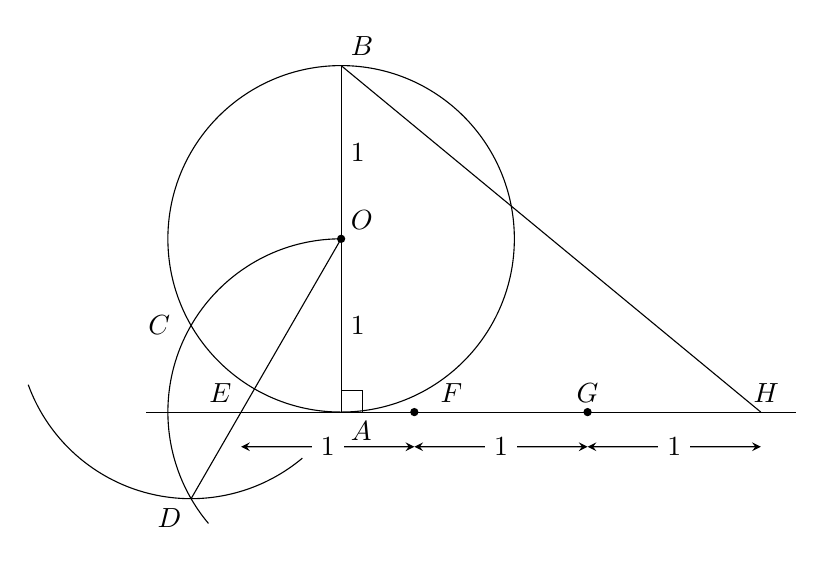
\begin{tikzpicture}[scale=.55]
% Scale at 4

% Coordinates of circle
\coordinate (O) at (0,0);
\coordinate (A) at (0,-4);
\coordinate (B) at (0,4);
\node[above right] at (O) {$O$};
\vertex{O};
\node[below right] at (A) {$A$};
\node[above right] at (B) {$B$};
\draw (A) rectangle +(14pt,14pt);

% Draw circle and diameter
\node [draw,circle through=(A),name path=circle] at (O) {};
\draw (A) --  node[right] {$1$} (O) -- node[right] {$1$} (B);

% Draw tangent at A
\draw[name path=tangent] ($(A)+(-4.5,0)$) -- ($(A)+(10.5,0)$);

% Draw arc centered at A which intersects circle at C
\draw[name path=Aarc] (O)
   arc [start angle=90,end angle=220,radius=4];
\path[name intersections={of=circle and Aarc,by=C}];
\node[left,xshift=-4pt] at (C) {$C$};

% Draw arc centered at C which intersects the first arc at D
\draw[name path=Carc] ($(C)+(200:4)$)
   arc [start angle=200,end angle=310,radius=4];
\path[name intersections={of=Carc and Aarc,by=D}];
\node[below left] at (D) {$D$};

% Draw O--D which intersects the tangent at E
\draw[name path=OD] (O) -- (D);
\path[name intersections={of=tangent and OD,by=E}];
\node[above left] at (E) {$E$};

% Find point H at length 3 from E
\coordinate (F) at ($(E)+(4,0)$);
\vertex{F};
\node[above right,xshift=6pt] at (F) {$F$};
\coordinate (G) at ($(F)+(4,0)$);
\vertex{G};
\node[above] at (G) {$G$};
\coordinate (H) at ($(G)+(4,0)$);
\node[above,xshift=2pt] at (H) {$H$};

% Draw BH of length approximately pi
\draw (B) -- (H);

\draw[<->] ($(E)+(0,-.8)$) -- node[fill=white] {$1$} ($(F)+(0,-.8)$);
\draw[<->] ($(F)+(0,-.8)$) -- node[fill=white] {$1$} ($(G)+(0,-.8)$);
\draw[<->] ($(G)+(0,-.8)$) -- node[fill=white] {$1$} ($(H)+(0,-.8)$);

\end{tikzpicture}
\end{center}
\caption{Kocha\'{n}ski's approximation to $\pi$}\label{f.square-kochansky}
\end{figure}

\begin{figure}[t]
\begin{center}
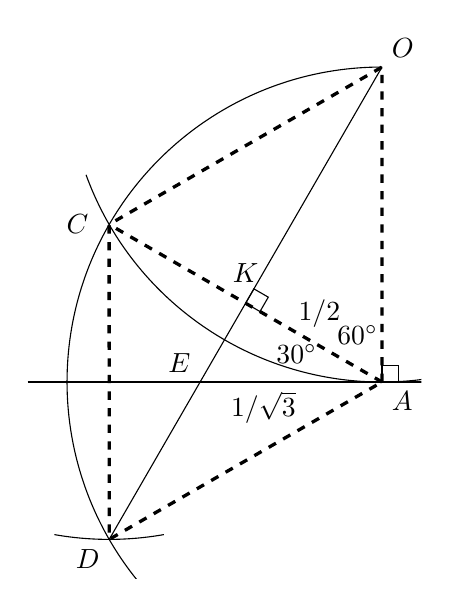
\begin{tikzpicture}[rotate=0,scale=1]
% Scale at 4

\clip (-4.5,-6.5) rectangle +(5,7);
% Coordinates of circle
\coordinate (O) at (0,0);
\coordinate (A) at (0,-4);
\coordinate (B) at (0,4);

% Draw circle
\node [circle through=(A),name path=circle] at (O) {};
\draw ($(O)+(200:4)$) arc [start angle=200,end angle=280,radius=4];

% Draw tangent at A
\draw[name path=tangent] ($(A)+(-4.5,0)$) -- ($(A)+(10.5,0)$);
\draw (A) rectangle +(6pt,6pt);

% Draw arc centered at O which intersects circle at C
\draw[name path=Aarc] (O)
   arc [start angle=90,end angle=220,radius=4];
\path[name intersections={of=circle and Aarc,by=C}];

% Draw arc centered at C which intersects the first arc at D
\draw[name path=Carc] ($(C)+(260:4)$)
   arc [start angle=260,end angle=280,radius=4];
\path[name intersections={of=Carc and Aarc,by=D}];

% Draw O--D which intersects the tangent at E
\draw[name path=OD] (O) -- (D);
\path[name intersections={of=tangent and OD,by=E}];

% Find point H at length 3 from E
\coordinate (F) at ($(E)+(4,0)$);
\coordinate (G) at ($(F)+(4,0)$);
\coordinate (H) at ($(G)+(4,0)$);

% Draw BH of length approximately pi
\draw (B) -- (H);

\draw[very thick,dashed] (A) -- (O) -- (C) -- (D) -- cycle;
\draw[very thick,dashed,name path=AC] (A) -- (C);

\node[above left,yshift=10pt,xshift=2pt] at (A) {$60^\circ$};
\node[left,yshift=10pt,xshift=-20pt] at (A) {$30^\circ$};

\path[name intersections={of=AC and OD,by=K}];
\draw[rotate=-30] (K) rectangle +(6pt,6pt);

\path (A) -- node[above,xshift=2pt,yshift=2pt] {$1/2$} (K);
\path (A) -- node[below,xshift=-10pt] {$1/\sqrt{3}$} (E);

\node[above right] at (O) {$O$};
\node[below right] at (A) {$A$};
\node[above right] at (B) {$B$};
\node[left,xshift=-4pt] at (C) {$C$};
\node[below left] at (D) {$D$};
\node[above left] at (E) {$E$};
\node[above] at (H) {$H$};
\node[above,yshift=4pt] at (K) {$K$};
\end{tikzpicture}
\end{center}
\caption[Detail from Kocha\'{n}ski's construction]{\vspace{-4ex}Detail from Kocha\'{n}ski's construction}\label{f.square-kochansky-detail}
\end{figure}

\begin{theorem}
$\quad\overline{BH}=\sqrt{\displaystyle\frac{40}{3}-2\sqrt{3}}\approx \pi$.
\end{theorem}
\begin{proof}
Figure~\ref{f.square-kochansky-detail} is an enlarged extract from Fig.~\ref{f.square-kochansky}, where dashed line segments have been added. Since all the circles are unit circles the lengths of the dashed lines are $1$. It follows that  $\overline{AOCD}$ is a rhombus so its diagonals are perpendicular to and bisect each other at the point labeled $K$. $\overline{AK}=1/2$.

\newpage

The diagonal $\overline{AC}$ forms two equilateral triangles $\triangle OAC, \triangle DAC$ so $\angle OAC=60^\circ$. Since the tangent forms a right angle with the radius $\overline{OA}$, $\angle KAE=30^\circ$. Now:
\begin{displaymath}
\renewcommand{\arraystretch}{1.5}
\begin{array}{lcl}
\displaystyle\frac{1/2}{\overline{EA}}&=&
\cos 30^\circ=\displaystyle\frac{\sqrt{3}}{2}\\
\overline{EA}&=&\displaystyle\frac{1}{\sqrt{3}}\\
\overline{AH}&=&3-\overline{EA}=\left(3-\displaystyle\frac{1}{\sqrt{3}}\right)
=\displaystyle\frac{3\sqrt{3}-1}{\sqrt{3}}\,.
\end{array}
\end{displaymath}

$\triangle ABH$ is a right triangle and $\overline{AH}=3-\overline{EA}$, so by Pythagoras's Theorem:
\begin{displaymath}
\renewcommand{\arraystretch}{1.5}
\begin{array}{lcl}
\overline{BH}^2&=&\overline{AB}^2+\overline{AH}^2\\
&=&4+\displaystyle\frac{27 -6\sqrt{3}+1}{3}=\frac{40}{3}-2\sqrt{3}\\
\overline{BH}&=&\rule{0pt}{25pt}\sqrt{\displaystyle\frac{40}{3}-2\sqrt{3}}\approx 3.141533387\approx \pi\,.
\end{array}
\end{displaymath}
\end{proof}


%%%%%%%%%%%%%%%%%%%%%%%%%%%%%%%%%%%%%%%%%%%%%%%%%%%%%%%%%%%%%%
\newpage

\section{Ramanujan's First Construction}\label{s.square-ramanujan-first}
\index{Ramanujan}\index{Squaring a circle!approximation}

\textbf{Construction (Fig.~\ref{f.square-rama1a}):}
\begin{enumerate}

\item Construct a unit circle centered at $O$ and let $\overline{PR}$ be a diameter.

\item Construct the point $H$ that bisects $\overline{PO}$ and the point $T$ that trisects $\overline{RO}$ (Thm.~\ref{thm.trisect-constructible}).

\item Construct the  perpendicular at $T$ that intersects the circle at $Q$.

\item Construct the chords $\overline{RS}=\overline{QT}$ and $\overline{PS}$.

\item Construct a line parallel to $\overline{RS}$ from $T$ that intersects $\overline{PS}$ at $N$.

\item Construct a line parallel to $\overline{RS}$ from $O$ that intersects $\overline{PS}$ at $M$.

\item Construct the chord $\overline{PK}=\overline{PM}$.

\item Construct the tangent at $P$ of length $\overline{PL}=\overline{MN}$.

\item Connect the points $K,L,R$.

\item Find point $C$ such that $\overline{RC}$ is equal to $\overline{RH}$.

\item Construct $\overline{CD}$ parallel to $\overline{KL}$ that intersects $\overline{LR}$ at $D$. 
\end{enumerate}

\begin{figure}[b]
\begin{center}
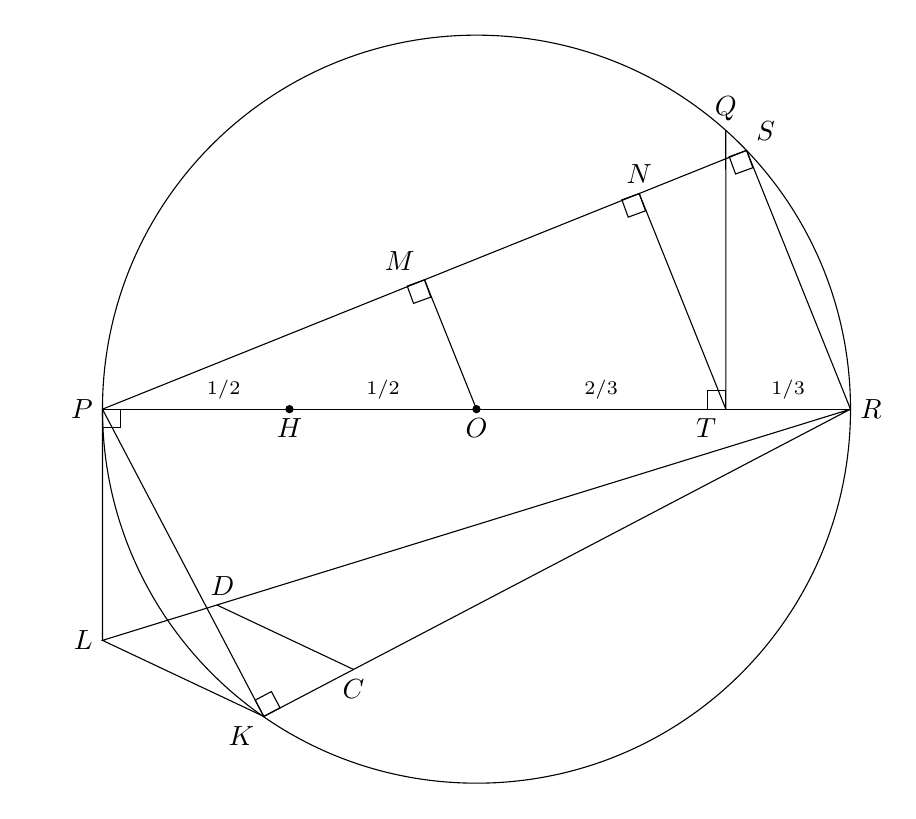
\begin{tikzpicture}[scale=.95,align=left]
\clip (-6,-5.1) rectangle +(11.5,10.2);
% Draw circle and horizontal diameter
\draw[name path=circle] (0,0)  coordinate (o) node[below] {$O$} circle[radius=5cm];
\draw (-5,0) coordinate (p) node[left] {$P$} -- (5,0) coordinate (r) node[right] {$R$};
\vertex{o};
\coordinate (h) at (-2.5,0);
\node[below] at (h) {$H$};
\vertex{h};
\coordinate (t) at (10/3,0);
\node[below left] at (t) {$T$};
\path (p) -- node[above,xshift=10pt] {\sm{1/2}} (h) -- node[above] {\sm{1/2}} (o) -- node[above] {\sm{2/3}} (t) -- node[above] {\sm{1/3}} (r);

% Draw perpendicular TQ
\path[name path=tq] (t) -- +(0,5);
\path[name intersections={of=tq and circle,by=q}];
\draw (t) -- (q) node[above] {$Q$};

% Draw chord RS and line PS
\path[name path=tq] (t) -- +(0,5);
\path[name intersections={of=tq and circle,by=q}];
\path[name path=rcirc] (r) let \p1 = ($ (t) - (q) $) in circle ({veclen(\x1,\y1)});
\path[name intersections={of=rcirc and circle,by=s}];
\draw (r) -- (s) node[above right] at (s) {$S$};
\draw[name path=ps] (p) -- (s);

% Draw TN
\path[name path=tn] (t) -- +($(s)-(r)$);
\path[name intersections={of=ps and tn,by=n}];
\draw (t) -- (n) node[above] {$N$};


% Draw OM
\path[name path=om] (o) -- +($(s)-(r)$);
\path[name intersections={of=ps and om,by=m}];
\draw (o) -- (m) node[above left] {$M$};
\path (p) -- (m);
\path (m) -- (n);

% Draw chord PK
\draw (p) -- +(-62.3:4.64) coordinate (k) node[below left] {$K$};

% Draw tangent PL
\draw let \p1 = ($ (m) - (n) $), \n1 = {veclen(\x1,\y1)} in (p) -- (-5,-\n1) coordinate (l) node[left] {$L$};

% Connect L and K to R
\draw (r) -- (l) -- (k) -- cycle;

% Find point C on RK
\coordinate (c) at ($(r)!7.5cm!(k)$);
\path (r) -- (c);
\node[below] at (c) {$C$};

% Draw CD
\path[name path=cd] (c) -- +($(l)-(k)$);
\path[name path=lr] (l) -- (r);
\path[name intersections={of=cd and lr,by=d}];
\draw (c) -- (d);
\node[above,xshift=2pt] at (d) {$D$};
\path (r) -- (d);

\draw[rotate=90] (t) rectangle +(7pt,7pt);
\draw[rotate=-90] (p) rectangle +(7pt,7pt);
\draw[rotate=-160] (s) rectangle +(7pt,7pt);
\draw[rotate=-160] (n) rectangle +(7pt,7pt);
\draw[rotate=-160] (m) rectangle +(7pt,7pt);
\draw[rotate=28] (k) rectangle +(7pt,7pt);
\end{tikzpicture}
\end{center}
\caption{Ramanujan's first construction}\label{f.square-rama1a}
\end{figure}

\begin{theorem}
$\quad\overline{RD}^2=\displaystyle\frac{355}{113}\approx \pi$.
\end{theorem}


\begin{proof}
$\overline{RS}=\overline{QT}$ by construction and by Pythagoras's Theorem for $\triangle QOT$:
\[
\overline{RS} =\overline{QT} =\sqrt{1^2-\left(\frac{2}{3}\right)^2}=\frac{\sqrt{5}}{3}\,.
\]
$\angle PSR$ is subtended by a diameter so $\triangle PSR$ is a right triangle. By Pythagoras's theorem:
\[
\overline{PS} = \sqrt{2^2-\left(\frac{\sqrt{5}}{3}\right)^2}=\sqrt{4-\frac{5}{9}}=\frac{\sqrt{31}}{3}\,.
\]
By construction $\overline{MO}\parallel \overline{RS}$ so
$\triangle MPO\sim \triangle SPR$ and:
%
\begin{eqnarray*}
\frac{\overline{PM}}{\overline{PO}}&=&\frac{\overline{PS}}{\overline{PR}}\\
\frac{\overline{PM}}{1}&=&\frac{\sqrt{31}/3}{2}\\
\overline{PM}&=&\frac{\sqrt{31}}{6}\,.
\end{eqnarray*}
By construction $\overline{NT}\parallel \overline{RS}$ so 
$\triangle NPT\sim \triangle SPR$ and:
\begin{eqnarray*}
\frac{\overline{PN}}{\overline{PT}}&=&\frac{\overline{PS}}{\overline{PR}}\\
\frac{\overline{PN}}{5/3}&=&\frac{\sqrt{31}/3}{2}\\
\overline{PN}&=&\frac{5\sqrt{31}}{18}\\
\overline{MN}&=&\overline{PN}-\overline{PM}=\sqrt{31}\left(\frac{5}{18}-\frac{1}{6}\right) = \frac{\sqrt{31}}{9}\,.
\end{eqnarray*}
$\triangle PKR$ is a right triangle because $\angle PKR$ is subtended by a diameter. By construction $\overline{PK}=\overline{PM}$ and by Pythagoras's Theorem:
\[
\overline{RK}=\sqrt{2^2-\left(\frac{\sqrt{31}}{6}\right)^2} = \frac{\sqrt{113}}{6}\,.
\]
$\triangle LPR$ is a right triangle because $\overline{PL}$ is a tangent so $\angle LPR$ is a right angle. $\overline{PL}=\overline{MN}$ by construction and by Pythagoras's Theorem:
\[
\overline{RL}=\sqrt{2^2+\left(\frac{\sqrt{31}}{9}\right)^2} = \frac{\sqrt{355}}{9}\,.
\]
By construction
$\overline{RC}=\overline{RH}=3/2$ and $\overline{CD} \parallel \overline{LK}$. By similar triangles:
%
\begin{eqnarray*}
\frac{\overline{RD}}{\overline{RC}}&=&\frac{\overline{RL}}{\overline{RK}}\\
\frac{\overline{RD}}{3/2}&=&\frac{\sqrt{355}/9}{\sqrt{113}/6}\\
\overline{RD}&=&\sqrt{\frac{355}{113}}\\
\overline{RD}^2&=&\frac{355}{113}\approx 3.14159292035\approx \pi\,.
\end{eqnarray*}
In Fig.~\ref{f.square-rama1b} the line segments are labeled with their lengths.
\end{proof}

\begin{figure}[ht]
\begin{center}
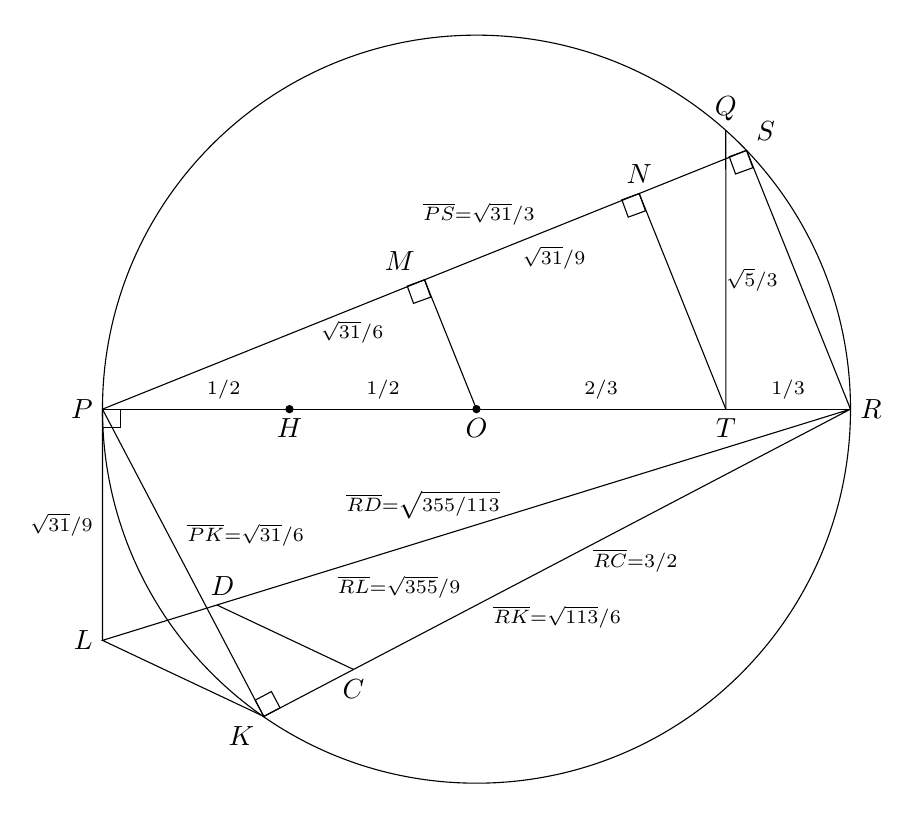
\begin{tikzpicture}[scale=.95,align=left]
\clip (-6,-5.1) rectangle +(11.5,10.2);
% Draw circle and horizontal diameter
\draw[name path=circle] (0,0)  coordinate (o) node[below] {$O$} circle[radius=5cm];

\draw (-5,0) coordinate (p) node[left] {$P$} -- (5,0) coordinate (r) node[right] {$R$};
\vertex{o};
\coordinate (h) at (-2.5,0);
\node[below] at (h) {$H$};
\vertex{h};
\coordinate (t) at (10/3,0);
\node[below] at (t) {$T$};

% Draw perpendicular TQ
\path[name path=tq] (t) -- +(0,5);
\path[name intersections={of=tq and circle,by=q}];
\draw (t) -- (q) node[above] {$Q$};


\path (p) -- node[above,xshift=10pt] {\sm{1/2}} (h) -- node[above] {\sm{1/2}} (o) -- node[above] {\sm{2/3}} (t) -- node[above] {\sm{1/3}} (r);
% Draw chord RS and line PS
\path[name path=tq] (t) -- +(0,5);
\path[name intersections={of=tq and circle,by=q}];
\path[name path=rcirc] (r) let \p1 = ($ (t) - (q) $) in circle ({veclen(\x1,\y1)});
\path[name intersections={of=rcirc and circle,by=s}];
\draw (r) -- node[left,xshift=-4pt] {\sm{\sqrt{5}/3}} (s);
\node[above right] at (s) {$S$};
\draw[name path=ps] (p) -- node[above right,xshift=-4pt,yshift=16pt] {\sm{\overline{PS}=\sqrt{31}/3}} (s);
% Draw TN
\path[name path=tn] (t) -- +($(s)-(r)$);
\path[name intersections={of=ps and tn,by=n}];
\draw (t) -- (n) node[above] {$N$};
% Draw OM
\path[name path=om] (o) -- +($(s)-(r)$);
\path[name intersections={of=ps and om,by=m}];
\draw (o) -- (m) node[above left] {$M$};
\path (p) -- node[below,xshift=32pt,yshift=12pt] {\sm{\sqrt{31}/6}} (m);
\path (m) -- node[below,xshift=8pt,yshift=0pt] {\sm{\sqrt{31}/9}} (n);
% Draw chord PK
\draw (p) -- node[right,xshift=-2pt,yshift=10pt] {\sm{\overline{PK}=\sqrt{31}/6}} +(-62.3:4.64) coordinate (k) node[below left] {$K$};
% Draw tangent PL
\draw let \p1 = ($ (m) - (n) $), \n1 = {veclen(\x1,\y1)} in (p) -- node[left] {\sm{\sqrt{31}/9}} (-5,-\n1) coordinate (l) node[left] {$L$};
% Connect L and K to R
\draw (r) -- (l) -- (k) -- cycle;
% Find point C on RK
\coordinate (c) at ($(r)!7.5cm!(k)$);
\path (r) -- node[below,xshift=12pt,yshift=0pt] {\sm{\overline{RC}=3/2}} (c);
\path (r) -- node[below,xshift=0pt,yshift=-12pt] {\sm{\overline{RK}=\sqrt{113}/6}} (k);
\node[below] at (c) {$C$};
% Draw CD
\path[name path=cd] (c) -- +($(l)-(k)$);
\path[name path=lr] (l) -- (r);
\path[name intersections={of=cd and lr,by=d}];
\draw (c) -- (d);
\node[above,xshift=2pt] at (d) {$D$};
\path (r) -- node[above,xshift=-40pt,yshift=-8pt] {\sm{\overline{RD}=\sqrt{355/113}}} (d);
\path (r) -- node[below,xshift=-28pt,yshift=-15pt] {\sm{\overline{RL}=\sqrt{355}/9}} (l);
\draw[rotate=28] (k) rectangle +(7pt,7pt);
\draw[rotate=-160] (s) rectangle +(7pt,7pt);
\draw[rotate=-160] (n) rectangle +(7pt,7pt);
\draw[rotate=-160] (m) rectangle +(7pt,7pt);
\draw[rotate=-90] (p) rectangle +(7pt,7pt);
\end{tikzpicture}
\end{center}
\caption{Ramanujan's first construction with labeled line segments}\label{f.square-rama1b}
\end{figure}

%%%%%%%%%%%%%%%%%%%%%%%%%%%%%%%%%%%%%%%%%%%%%%%%%%%%%%%%%%%%
\newpage

\section{Ramanujan's Second Construction}\label{s.square-ramanujan-second}
\index{Ramanujan}\index{Squaring a circle!approximation}

\textbf{Construction  (Fig.~\ref{f.square-ramanujan-2a}):}
\begin{enumerate}

\item Construct a unit circle centered at $O$ with diameter $\overline{AB}$ and let $C$ be the intersection of the perpendicular to $\overline{AB}$ at $O$ with the circle.

\item Trisect the line segment $\overline{AO}$ such that $\overline{AT}=1/3$ and $\overline{TO}=2/3$ (Thm.~\ref{thm.trisect-constructible}).

\item Construct $\overline{BC}$ and find points $M,N$ such that $\overline{CM}=\overline{MN}=\overline{AT}=1/3$.

\item Construct $\overline{AM}$, $\overline{AN}$ and let $P$ be the point on $\overline{AN}$ such that $\overline{AP}=\overline{AM}$.

\item From $P$ construct a line parallel to $\overline{MN}$ that intersects $\overline{AM}$ at $Q$.

\item Construct $\overline{OQ}$ and then from $T$ construct a line parallel to $\overline{OQ}$ that intersects $\overline{AM}$ at $R$.

\item Construct $\overline{AS}$ tangent to $A$ such that $\overline{AS}=\overline{AR}$.

\item Construct $\overline{SO}$.
\end{enumerate}

\begin{figure}[ht]
\begin{center}
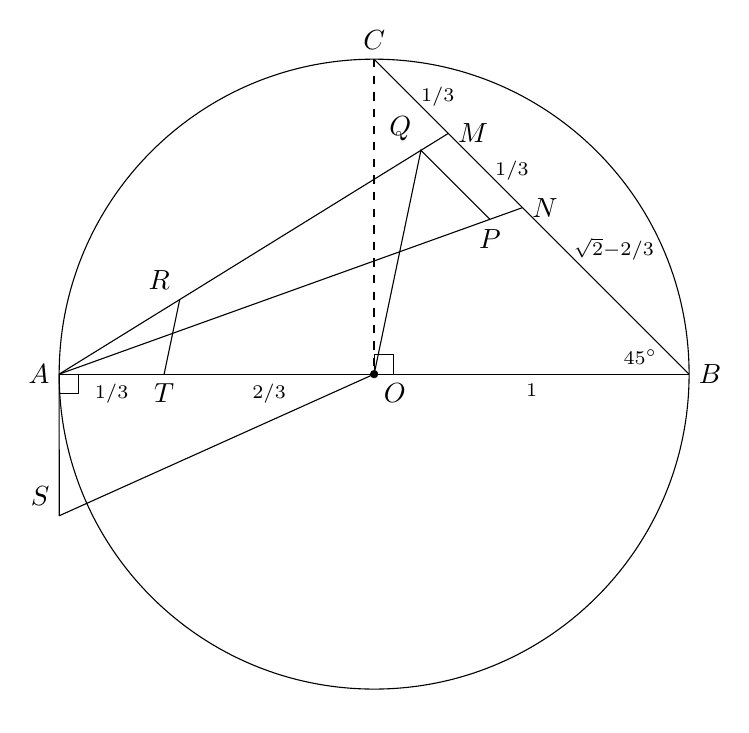
\begin{tikzpicture}[scale=1]
\clip (-4.4,-4.2) rectangle +(8.8,8.6);
% Scale at 4

% Coordinates of circle
\coordinate (O) at (0,0);
\vertex{O};
\coordinate (A) at (-4,0);
\coordinate (B) at (4,0);
\coordinate (C) at (0,4);

% Draw circle and diameter
\node [draw,circle through=(A),name path=circle] at (O) {};
\draw (A) -- (B);
\draw [thick,dashed] (C) -- (O);
\draw (O) rectangle +(7pt,7pt);
\draw[rotate=-90] (A) rectangle +(7pt,7pt);

\coordinate (T) at (-2.667,0);
\path (A) -- node[below] {\sm{1/3}} (T);
\path (T) -- node[below] {\sm{2/3}} (O);
\path (O) -- node[below] {\sm{1}} (B);

\draw (C) -- node[right] {\sm{1/3}} +(-45:1.333) coordinate (M);
\draw (M) -- node[right] {\sm{1/3}} +(-45:1.333) coordinate (N);
\draw (N) -- node[near start,right] {\sm{\sqrt{2}-2/3}}(B);

\draw[name path=AM] (A) -- (M);
\draw[name path=AN] (A) -- (N);

\node [circle through=(M),name path=AMcircle] at (A) {};

\path[name intersections={of=AMcircle and AN,by=P}];

\path[name path=PQ] (P) -- +(135:2);
\path[name intersections={of=PQ and AM,by=Q}];
\draw (P) -- (Q) -- (O);

\path[name path=QT] (T) -- ($(Q)+(-2.667,0)$) -- (Q);
\path[name intersections={of=QT and AM,by=R}];
\draw (T) -- (R);

\node [circle through=(R),name path=ARcircle] at (A) {};
\path[name path=AS] (A) -- ($(A)+(0,-2.5)$);
\path[name intersections={of=ARcircle and AS,by=S}];
\draw (A) -- (S);

\draw (S) -- (O);

\node[below right] at (O) {$O$};
\node[left] at (A) {$A$};
\node[right] at (B) {$B$};
\node[above left,xshift=-8pt] at (B) {\sm{45^\circ}};
\node[above] at (C) {$C$};
\node[below] at (T) {$T$};
\node[right] at (M) {$M$};
\node[right] at (N) {$N$};
\node[below] at (P) {$P$};
\node[above left] at (Q) {$Q$};
\node[above left] at (R) {$R$};
\node[above left] at (S) {$S$};
\end{tikzpicture}
\end{center}
\caption{Ramanujan's second construction}\label{f.square-ramanujan-2a}
\end{figure}

\newpage

\begin{theorem}\label{thm.ramanujan2}
$\quad 3\sqrt{\overline{SO}}=\left(9^2+\displaystyle\frac{19^2}{22}\right)^{1/4}\approx \pi$.
\end{theorem}
\begin{proof}
$\triangle COB$ is a right triangle so by Pythagoras's Theorem $\overline{CB}=\sqrt{2}$ and:
\[
\overline{NB}=\sqrt{2}-2/3\,.
\]
$\triangle COB$ is isoceles so $\angle NBA =\angle MBA=45^\circ$. By the Law of Cosines\index{Law of cosines}:
\begin{eqnarray*}
\overline{AN}^2&=&\overline{BA}^2 + \overline{BN}^2-2\cdot\overline{BA}\cdot\overline{BN}\cdot\cos \angle NBA\\
&=&2^2+\left(\sqrt{2}-\frac{2}{3}\right)^2-2\cdot 2 \cdot \left(\sqrt{2}-\frac{2}{3}\right)\cdot \frac{\sqrt{2}}{2}
%&=&\left(4+2+\frac{4}{9}-4\right) + \sqrt{2}\cdot \left(-\frac{4}{3}+\frac{4}{3}\right)
=\frac{22}{9}\\
\overline{AN}&=&\sqrt{\frac{22}{9}}\,.
\end{eqnarray*}
Again by the Law of Cosines\index{Law of cosines}:
\begin{eqnarray*}
\overline{AM}^2&=&\overline{BA}^2 + \overline{BM}^2-2\cdot\overline{BA}\cdot\overline{BM}\cdot\cos \angle MBA\\
&=&2^2+\left(\sqrt{2}-\frac{1}{3}\right)^2-2\cdot 2 \cdot \left(\sqrt{2}-\frac{1}{3}\right)\cdot \frac{\sqrt{2}}{2}
%&=&\left(4+2+\frac{1}{9}-4\right) + \sqrt{2}\cdot \left(-\frac{2}{3}+\frac{2}{3}\right)
=\frac{19}{9}\\
\overline{AM}&=&\sqrt{\frac{19}{9}}\,.
\end{eqnarray*}
By construction $\overline{QP}\parallel  \overline{MN}$ so
$\triangle MAN\sim \triangle QAP$, and by construction $\overline{AP}=\overline{AM}$:
\begin{eqnarray*}
\frac{\overline{AQ}}{\overline{AM}}&=&\frac{\overline{AP}}{\overline{AN}}=\frac{\overline{AM}}{\overline{AN}}\\
\overline{AQ}&=&\frac{\overline{AM}^2}{\overline{AN}}=\frac{19/9}{\sqrt{22/9}}=\frac{19}{3\sqrt{22}}\,.
\end{eqnarray*}
By construction $\overline{TR}\parallel  \overline{OQ}$ so
$\triangle RAT\sim \triangle QAO$ and:
\begin{eqnarray*}
\frac{\overline{AR}}{\overline{AQ}}&=&\frac{\overline{AT}}{\overline{AO}}\\
\overline{AR}&=&\overline{AQ}\cdot\frac{\overline{AT}}{\overline{AO}}=\frac{19}{3\sqrt{22}}\cdot\frac{1/3}{1}=\frac{19}{9\sqrt{22}}\,.
\end{eqnarray*}

\newpage

By construction $\overline{AS}=\overline{AR}$ and $\triangle OAS$ is a right triangle because $\overline{AS}$ is a tangent. By Pythagoras's Theorem:
\begin{eqnarray*}
\overline{SO}&=&\sqrt{1^2+\left(\frac{19}{9\sqrt{22}}\right)^2}\\
3\sqrt{\overline{SO}}&=&3\left(1^2+\frac{19^2}{9^2\cdot 22}\right)^{1/4}=
\left(9^2+\frac{19^2}{22}\right)^{1/4}\approx 3.14159265258\approx\pi\,.
\end{eqnarray*}
\enlargethispage{\baselineskip}
In Fig.~\ref{f.square-ramanujan-2b} the line segments are labeled with their lengths.
\end{proof}


\begin{figure}[ht]
\begin{center}
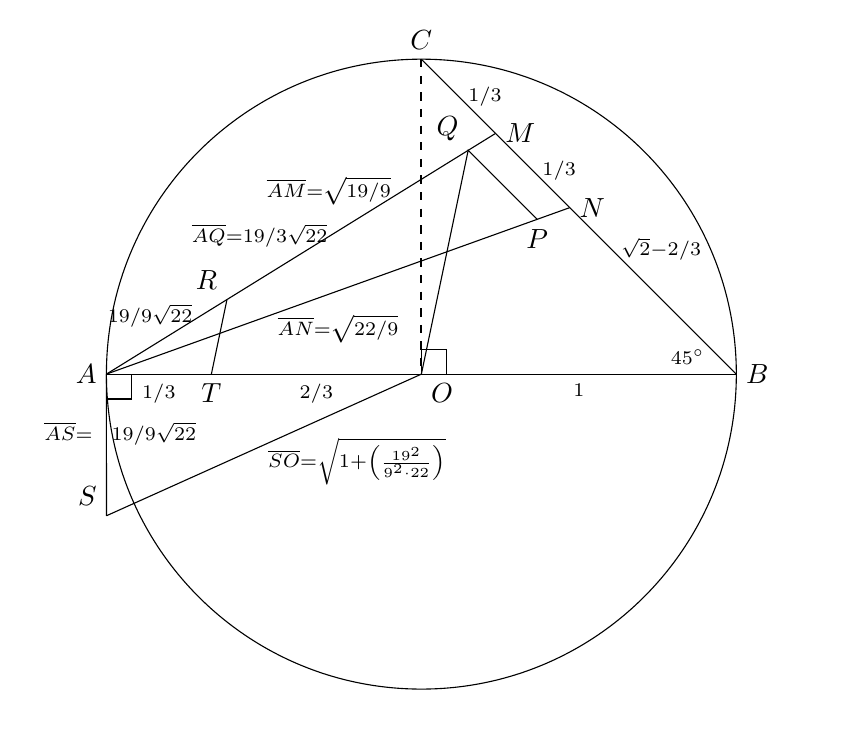
\begin{tikzpicture}[scale=1]
\clip (-5,-4.2) rectangle +(10,8.6);
% Scale at 4

% Coordinates of circle
\coordinate (O) at (0,0);
\coordinate (A) at (-4,0);
\coordinate (B) at (4,0);
\coordinate (C) at (0,4);

% Draw circle and diameter
\node [draw,circle through=(A),name path=circle] at (O) {};
\draw (A) -- (B);
\draw [thick,dashed] (C) -- (O);
\draw (O) rectangle +(9pt,9pt);
\draw[rotate=-90] (A) rectangle +(9pt,9pt);

\coordinate (T) at (-2.667,0);
\path (A) -- node[below] {\sm{1/3}} (T);
\path (T) -- node[below] {\sm{2/3}} (O);
\path (O) -- node[below] {\sm{1}} (B);

\draw (C) -- node[right] {\sm{1/3}} +(-45:1.333) coordinate (M);
\draw (M) -- node[right] {\sm{1/3}} +(-45:1.333) coordinate (N);
\draw (N) -- node[near start,right] {\sm{\sqrt{2}-2/3}}(B);

\draw[name path=AM] (A) -- node[above,xshift=10pt,yshift=14pt] {\sm{\overline{AM}=\sqrt{19/9}}} (M);
\draw[name path=AN] (A) -- node[below,yshift=-5pt] {\sm{\overline{AN}=\sqrt{22/9}}} (N);

\node [circle through=(M),name path=AMcircle] at (A) {};

\path[name intersections={of=AMcircle and AN,by=P}];

\path[name path=PQ] (P) -- +(135:2);
\path[name intersections={of=PQ and AM,by=Q}];
\draw (P) -- (Q) -- (O);
\path (A) -- node[above,xshift=-10pt,yshift=2pt] {\sm{\overline{AQ}=19/3\sqrt{22}}} (Q);

\path[name path=QT] (T) -- ($(Q)+(-2.667,0)$) -- (Q);
\path[name intersections={of=QT and AM,by=R}];
\draw (T) -- (R);
\path (A) -- node[above,xshift=-6pt,yshift=0pt] {\sm{19/9\sqrt{22}}} (R);

\node [circle through=(R),name path=ARcircle] at (A) {};
\path[name path=AS] (A) -- ($(A)+(0,-2.5)$);
\path[name intersections={of=ARcircle and AS,by=S}];
\draw (A) -- node[xshift=5pt,yshift=4pt] {\sm{\overline{AS}=\;\;\;19/9\sqrt{22}}} (S);

\draw (S) -- node[right,xshift=-2pt,yshift=-6pt] {\sm{\overline{SO}=\sqrt{1+\left(\frac{19^2}{9^2\cdot 22}\right)}}} (O);
\node[below right] at (O) {$O$};
\node[left] at (A) {$A$};
\node[right] at (B) {$B$};
\node[above left,xshift=-8pt] at (B) {\sm{45^\circ}};
\node[above] at (C) {$C$};
\node[below] at (T) {$T$};
\node[right] at (M) {$M$};
\node[right] at (N) {$N$};
\node[below] at (P) {$P$};
\node[above left] at (Q) {$Q$};
\node[above left] at (R) {$R$};
\node[above left] at (S) {$S$};
\end{tikzpicture}
\end{center}
\caption{Ramanujan's second construction with labeled line segments}\label{f.square-ramanujan-2b}
\end{figure}


%%%%%%%%%%%%%%%%%%%%%%%%%%%%%%%%%%%%%%%%%%%%%%%%%%%%%%%%%%%%%

\newpage

\section{Squaring a Circle Using a Quadratrix}\label{s.square-quad}
\index{Squaring a circle!quadratrix@with a quadratrix}
\index{Quadratrix!squaring a circle}

The quadratrix is described in Sect.~\ref{s.q}.

Let $t=\overline{DE}$ be the distance that the horizontal straightedge has moved down the $y$-axis, and let $\theta$ be the corresponding angle between the rotating straightedge and the $x$-axis. Let $P$ the position of the joint of the two straightedges. The locus of $P$ is the quadratrix curve.

Let $F$ be the projection of $P$ onto the $x$-axis and let $G$ be the position of the joint when both straightedges reach the $x$-axis, that is, $G$ is the intersection of the quadratrix curve and the $x$-axis  (Fig.~\ref{f.square-quad}).
\begin{figure}[ht]
\begin{center}
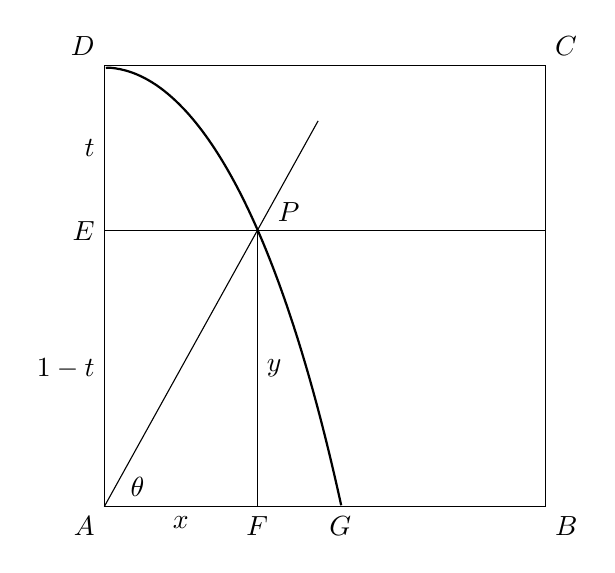
\begin{tikzpicture}[scale=.7,domain=.01:1.57,samples=100]
\draw (0,0) node[below left] {$A$} node [above right,xshift=6pt] {$\theta$} -- (8,0) node[below right] {$B$} -- (8,8) node[above right] {$C$} -- (0,8) node[above left] {$D$} -- cycle;
\draw[name path=horiz] (0,5) -- (8,5);
\draw[name path=slant] (0,0) -- (61:8);
\path[name intersections={of=horiz and slant,by=joint}];
\draw (joint) -- node[right] {$y$} (joint |- 0,0) coordinate (f);
\path (0,0) -- node[below] {$x$} (0,0 -| joint) node[below] {$F$};
\coordinate (e) at (0,5);
\path (e) node[left] {$E$} -- node[left] {$t$} (0,8);
\path (0,0) -- node[left] {$1-t$} (0,5);
\node[above right,xshift=4pt] at (joint) {$P$};
\node[below] at (4.28,0) {$G$};
\draw[name path=curve,thick] plot (4.3*.637*\x,{12.5*.637*\x*cot(\x r)});
\end{tikzpicture}
\end{center}
\caption{Squaring the circle with a quadratrix}\label{f.square-quad}
\end{figure}

\begin{theorem}
$\quad\overline{AG}=2/\pi$.
\end{theorem}

\begin{proof}
Let $y=\overline{PF}=\overline{EA}=1-t$. Since on a quadratrix $\theta$ decreases at the same rate that $t$ increases:
\begin{eqnarray*}
\frac{1-t}{1} &=& \frac{\theta}{\pi/2}\\
&&\\
\theta &=&\frac{\pi}{2}(1-t)\,.
\end{eqnarray*}
Let $x=\overline{AF}=\overline{EP}$. Then $\tan \theta = y/x$ so:
\begin{align}\label{eq.quad-square}
x = \frac{y}{\tan\theta}=y\cot\theta=y\cot \frac{\pi}{2}(1-t)=y\cot \frac{\pi}{2}y\,.
\end{align}
We usually express a function as $y=f(x)$ but it can also be expressed as $x=f(y)$. 

To obtain $x=\overline{AG}$ we can't simply plug $y=0$ into Eq.~\ref{eq.quad-square}, because $\cot 0$ is not defined, so let us compute the limit of $x$ as $y$ goes to $0$. 
First perform the substitution $z=(\pi/2)y$ to obtain:
\[
x = y\cot \frac{\pi}{2}y = \frac{2}{\pi} \left(\frac{\pi}{2}y\cot \frac{\pi}{2}y\right)=\frac{2}{\pi}(z\cot z)\,,
\]
and then take the limit:
\[
\lim_{z\rightarrow 0} x=\frac{2}{\pi}\lim_{z\rightarrow 0} (z\cot z) = \frac{2}{\pi}\lim_{z\rightarrow 0} \left(\frac{z\cos z}{\sin z}\right) = \frac{2}{\pi}\lim_{z\rightarrow 0} \left(\frac{\cos z}{(\sin z)/z}\right) = \frac{2}{\pi}\frac{\cos 0}{1} = \frac{2}{\pi}\,,
\]
where we have used $\lim_{z\rightarrow 0} (\sin z/z)=1$ (Thm.~\ref{thm.limit-sine-over}).
\end{proof}

\subsection*{What Is the Surprise?}

It is surprising that such accurate approximations to $\pi$ can be constructed. Of course one can't help but be astonished by Ramanujan's clever constructions.

\subsection*{Sources}
Kocha\'{n}ski's construction appears in \cite{bold}. Ramanujan's constructions are from \cite{ramanujan1,ramanujan2}. Squaring the circle using the quadratrix is from \cite[pp.~48--49]{martin} and \cite{wiki:quad}.


\tikzsetfigurename{five}
% !TeX root = surprises.tex

\chapter{El teorema de los cinco colores}\label{c.five}

%%%%%%%%%%%%%%%%%%%%%%%%%%%%%%%%%%%%%%%%%%%%%%%%%%%%%%%%%%%%%%%

Los mapas utilizan colores para distinguir una región de otra, asegurándose de que las regiones adyacentes estén coloreadas con colores diferentes. En 1852, Francis Guthrie observó que un mapa de los condados de Inglaterra podía colorearse con sólo cuatro colores. La afirmación de que cuatro países bastan para colorear cualquier mapa plano se denomina teorema de los cuatro colores y no fue demostrada hasta 1976 por Kenneth Appel y Wolfgang Haken. Ellos utilizaron sofisticados argumentos matemáticos para demostrar que si existe un contraejemplo (un mapa que necesite más de cuatro colores), tiene que estar asociado a una de las $1834$ configuraciones. A continuación, utilizaron un ordenador para comprobar estas configuraciones.

Mientras que el teorema de los cuatro colores es extremadamente difícil de demostrar, las demostraciones de los teoremas de los cinco y seis colores son relativamente sencillas (Secs.~\ref{s.six-color}, ~\ref{s.five-color}). Para demostrar de estos teoremas, definimos mapas y grafos planares (Sec.~\ref{s.planar}), demostramos la fórmula de Euler (Sec.~\ref{s.euler}) y mostramos que un grafo planar debe tener vértices cuyo grado sea menor o igual que cinco. En la Sección~\ref{s.nonplanar} se utiliza la fórmula de Euler para demostrar que dos grafos no son planares.

En 1879 Alfred B. Kempe publicó una demostración del teorema de los cuatro colores, pero en 1890 Percy J. Heawood demostró que la demostración es incorrecta. En la Sección~\ref{s.kempe} presentamos la demostración errónea de Kempe y la demostración de Heawood de que no es correcta.

%%%%%%%%%%%%%%%%%%%%%%%%%%%%%%%%%%%%%%%%%%%%%%%%%%%%%%%%%%%

\section{Mapas y grafos planos}\label{s.planar}

\begin{definition}
Un \textit{mapa plano} es un conjunto de regiones en el plano separadas por fronteras. Una \textit{coloración} de un mapa es una asignación de un color a cada región de tal manera que se asignan diferentes colores a las regiones que tienen una frontera en común.
\end{definition}

La figura~\ref{f.five-planar-map-five} muestra una coloración con cinco colores de un mapa planar con diez regiones.
La figura~\ref{f.five-planar-map-four} muestra una coloración con cuatro colores del mismo mapa.

\begin{figure}[t]
\begin{minipage}{.45\textwidth}
\begin{center}
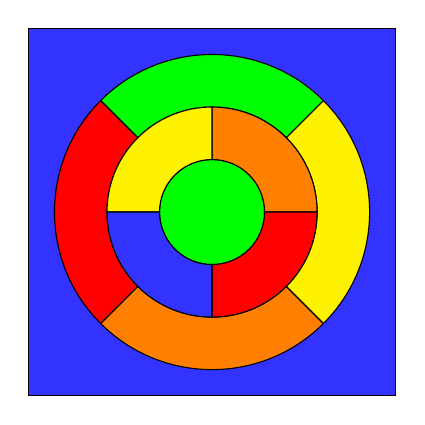
\begin{tikzpicture}[scale=.667]
\draw[fill=blue!80] (-3.5,-3.5) rectangle +(7,7);

\draw[fill=green] (0:1) 
  arc [start angle=0,  end angle=360, radius=1];

\draw[fill=green] (45:2) --
      (45:3)  arc[start angle=45,  end angle=135, radius=3] --
      (135:2) arc[start angle=135, end angle=45,  radius=2];
\draw[fill=orange] (-45:2) --
      (-45:3)  arc[start angle=-45,  end angle=-135, radius=3] --
      (-135:2) arc[start angle=-135, end angle=-45,  radius=2];
\draw[fill=yellow] (45:2) --
      (45:3)  arc[start angle=45,  end angle=-45, radius=3] --
      (-45:2) arc[start angle=-45, end angle=45,  radius=2];
\draw[fill=red] (135:2) --
      (135:3)  arc[start angle=135,  end angle=225, radius=3] --
      (225:2) arc[start angle=225, end angle=135,  radius=2];

\draw[fill=orange] (0:1) --
      (0:2)  arc[start angle=0,  end angle=90, radius=2] --
      (90:1) arc[start angle=90, end angle=0,  radius=1];
\draw[fill=red] (0:1) --
      (0:2)  arc[start angle=0,  end angle=-90, radius=2] --
      (-90:1) arc[start angle=-90, end angle=0,  radius=1];
\draw[fill=yellow] (90:1) --
      (90:2)  arc[start angle=90,  end angle=180, radius=2] --
      (180:1) arc[start angle=180, end angle=90,  radius=1];
\draw[fill=blue!80] (180:1) --
      (180:2)  arc[start angle=180,  end angle=270, radius=2] --
      (270:1) arc[start angle=270, end angle=180,  radius=1];
\end{tikzpicture}
\caption{Coloración de un mapa con cinco colores}\label{f.five-planar-map-five}
\end{center}
\end{minipage}
\hfill
\begin{minipage}{.45\textwidth}
\begin{center}
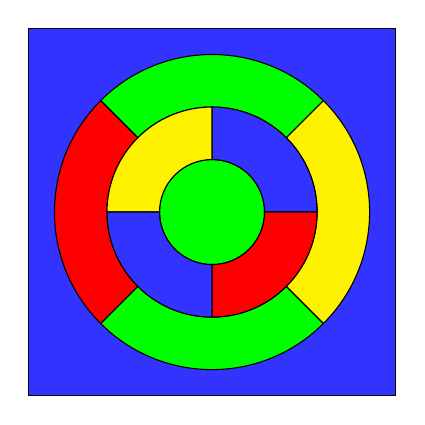
\begin{tikzpicture}[scale=.667]
\draw[fill=blue!80] (-3.5,-3.5) rectangle +(7,7);

\draw[fill=green] (0:1) 
  arc [start angle=0,  end angle=360, radius=1];

\draw[fill=green] (45:2) --
      (45:3)  arc[start angle=45,  end angle=135, radius=3] --
      (135:2) arc[start angle=135, end angle=45,  radius=2];
\draw[fill=green] (-45:2) --
      (-45:3)  arc[start angle=-45,  end angle=-135, radius=3] --
      (-135:2) arc[start angle=-135, end angle=-45,  radius=2];
\draw[fill=yellow] (45:2) --
      (45:3)  arc[start angle=45,  end angle=-45, radius=3] --
      (-45:2) arc[start angle=-45, end angle=45,  radius=2];
\draw[fill=red] (135:2) --
      (135:3)  arc[start angle=135,  end angle=225, radius=3] --
      (225:2) arc[start angle=225, end angle=135,  radius=2];

\draw[fill=blue!80] (0:1) --
      (0:2)  arc[start angle=0,  end angle=90, radius=2] --
      (90:1) arc[start angle=90, end angle=0,  radius=1];
\draw[fill=red] (0:1) --
      (0:2)  arc[start angle=0,  end angle=-90, radius=2] --
      (-90:1) arc[start angle=-90, end angle=0,  radius=1];
\draw[fill=yellow] (90:1) --
      (90:2)  arc[start angle=90,  end angle=180, radius=2] --
      (180:1) arc[start angle=180, end angle=90,  radius=1];
\draw[fill=blue!80] (180:1) --
      (180:2)  arc[start angle=180,  end angle=270, radius=2] --
      (270:1) arc[start angle=270, end angle=180,  radius=1];
\end{tikzpicture}
\caption{Coloración de un mapa con cuatro colores}\label{f.five-planar-map-four}
\end{center}
\end{minipage}
\end{figure}

\begin{definition}
Un \emph{grafo} es un conjunto de \emph{vértices} $V$ y un conjunto de \emph{aristas} $E$, tal que cada arista es incidente a exactamente dos vértices.

Un \emph{grafo plano} es un grafo en el que ninguna arista se cruza con otra. En un grafo plano, las zonas delimitadas por un conjunto de aristas se llaman \emph{caras (o regiones)}.

Una \emph{coloración} de un grafo plano es una asignación de colores a los vértices de tal manera que no hay dos vértices del mismo color conectados por una arista.
\end{definition}

Los mapas planos y los grafos planos son duales y, por lo tanto, es conveniente investigar los problemas de coloración en grafos en lugar de hacerlo directamente en mapas.

\begin{theorem}
Dado un mapa plano, se puede construir un grafo plano tal que para cada coloración de las regiones del mapa exista una coloración de los vértices del grafo, y a la inversa.
\end{theorem}

\begin{proof}
Construimos un vértice para cada región y una arista entre dos vértices si y sólo si las regiones correspondientes comparten un límite. 
\end{proof}

\begin{example}
La figura~\ref{f.five-planar-graph-map} muestra el mapa planar de la Fig.~\ref{f.five-planar-map-four} y los vértices asociados a las regiones. La figura~\ref{f.five-planar-graph-graph} muestra el grafo plano que corresponde al mapa.
\end{example}

\begin{figure}[t]
\begin{minipage}{.45\textwidth}
\begin{center}
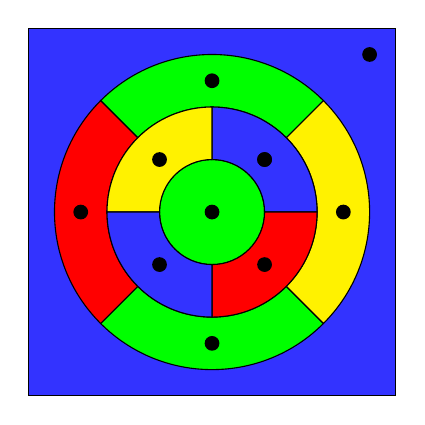
\begin{tikzpicture}[scale=.667]

\draw[fill=blue!80] (-3.5,-3.5) rectangle +(7,7);

\draw[fill=green] (0:1) 
  arc [start angle=0,  end angle=360, radius=1];

\draw[fill=green] (45:2) --
      (45:3)  arc[start angle=45,  end angle=135, radius=3] --
      (135:2) arc[start angle=135, end angle=45,  radius=2];
\draw[fill=green] (-45:2) --
      (-45:3)  arc[start angle=-45,  end angle=-135, radius=3] --
      (-135:2) arc[start angle=-135, end angle=-45,  radius=2];
\draw[fill=yellow] (45:2) --
      (45:3)  arc[start angle=45,  end angle=-45, radius=3] --
      (-45:2) arc[start angle=-45, end angle=45,  radius=2];
\draw[fill=red] (135:2) --
      (135:3)  arc[start angle=135,  end angle=225, radius=3] --
      (225:2) arc[start angle=225, end angle=135,  radius=2];

\draw[fill=blue!80] (0:1) --
      (0:2)  arc[start angle=0,  end angle=90, radius=2] --
      (90:1) arc[start angle=90, end angle=0,  radius=1];
\draw[fill=red] (0:1) --
      (0:2)  arc[start angle=0,  end angle=-90, radius=2] --
      (-90:1) arc[start angle=-90, end angle=0,  radius=1];
\draw[fill=yellow] (90:1) --
      (90:2)  arc[start angle=90,  end angle=180, radius=2] --
      (180:1) arc[start angle=180, end angle=90,  radius=1];
\draw[fill=blue!80] (180:1) --
      (180:2)  arc[start angle=180,  end angle=270, radius=2] --
      (270:1) arc[start angle=270, end angle=180,  radius=1];

\foreach \x/\y/\name in {
    0/0/O,
    3/3/Z,
    1/1/E,-1/1/F,-1/-1/G,1/-1/H,
    0/2.5/A,2.5/0/B,0/-2.5/C,-2.5/0/D,
    } {
  \fill (\x,\y) coordinate(\name) circle(4pt);
}
\end{tikzpicture}
\caption{Asociación de los vértices con las regiones de un mapa plano}\label{f.five-planar-graph-map}
\end{center}
\end{minipage}
\hfill
\begin{minipage}{.45\textwidth}
\begin{center}
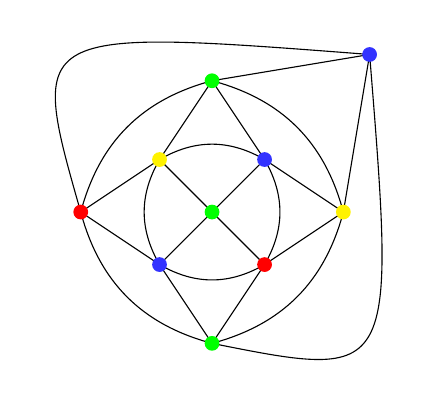
\begin{tikzpicture}[scale=.667]

\foreach \x/\y/\name in {
    0/0/O,
    3/3/Z,
    1/1/E,-1/1/F,-1/-1/G,1/-1/H,
    0/2.5/A,2.5/0/B,0/-2.5/C,-2.5/0/D,
    } {
  \coordinate(\name) at (\x,\y);
}

\draw (E) -- (O) -- (F);
\draw (G) -- (O) -- (H);
\draw (E) to [bend right=30] (F) to [bend right=30] (G) 
          to [bend right=30] (H) to [bend right=30] (E);
\draw (A) -- (E) -- (B) -- (H) -- (C) -- (G) -- (D) -- (F);
\draw (A) to [bend right=30] (D) to [bend right=30] (C) 
          to [bend right=30] (B) to [bend right=30] (A);

\draw (F) -- (A) -- (Z) -- (B);
\draw (C) .. controls (3.5,-3.2) .. (Z);
\draw (D) .. controls (-3.5,3.5) .. (Z);

\foreach \cl/\x/\y in {
    green/0cm/0cm,
    blue!80/3cm/3cm,
    blue!80/1cm/1cm,
    yellow/-1cm/1cm,
    blue!80/-1cm/-1cm,
    red/1cm/-1cm,
    green/0cm/2.5cm,
    yellow/2.5cm/0cm,
    green/0cm/-2.5cm,
    red/-2.5cm/0cm
    }
 \fill[\cl] (\x,\y) circle (4pt);
\end{tikzpicture}
\caption{El grafo plano que corresponde al mapa plano}\label{f.five-planar-graph-graph}
\end{center}
\end{minipage}
\end{figure}

Podemos limitar aún más nuestros grafos a aquellos cuyas caras son triangulares.

\begin{definition}
Un grafo es \emph{triangular} si todas sus caras están delimitadas por tres aristas. Un grafo puede ser \emph{triangulado} si se pueden añadir aristas de forma que el grafo sea triangular. También decimos que existe una \emph{triangulación} del grafo.
\end{definition}\index{Triangulated graph}

\begin{example}
Las caras del grafo plano de la Fig.~\ref{f.five-planar-graph-graph} son triangulares ya que cada una está delimitada por tres aristas. Las aristas son curvas por lo que las caras no son triángulos, que son polígonos cuyos tres lados son segmentos de línea recta.
\end{example}

\begin{advanced}
\textbf{El Teorema de F\'{a}ry} establece que cualquier grafo plano triangular puede transformarse en un grafo plano equivalente cuyas aristas sean segmentos de recta. Por lo tanto, sin pérdida de generalidad, las demostraciones se pueden restringir a grafos planos cuyas caras son triángulos.
\end{advanced}

\begin{example}
Fig.~\ref{f.five-triangular-graph} (izquierda) muestra que un cuadrado puede ser bicolor, pero si está triangulado (centro), son necesarios cuatro colores. Nuestro objetivo es demostrar que los grafos pueden ser coloreados con $n$ colores para algún $n$. Si el grafo triangulado está coloreado con $n$, también lo está el grafo original, porque eliminar las aristas sobrantes no invalida la coloración (derecha).
\end{example}

\begin{figure}[h]
\begin{center}
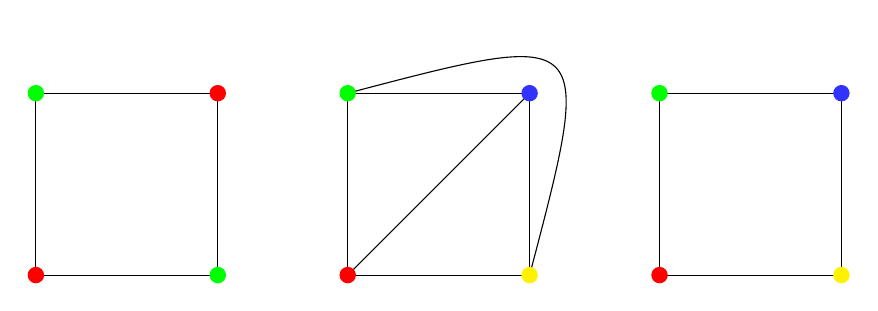
\begin{tikzpicture}[scale=.33]
\draw (-3.5,-3.5) rectangle +(7,7);
\fill[red] (-3.5,-3.5) circle(9pt);
\fill[green] (-3.5,3.5) circle(9pt);
\fill[green] (3.5,-3.5) circle(9pt);
\fill[red] (3.5,3.5) circle(9pt);
\begin{scope}[xshift=12cm]
\draw (-3.5,-3.5) -- (3.5,3.5);
\draw (-3.5,3.5) .. controls (6,6) .. (3.5,-3.5);
\draw (-3.5,-3.5) rectangle +(7,7);
\fill[red] (-3.5,-3.5) circle(9pt);
\fill[green] (-3.5,3.5) circle(9pt);
\fill[yellow] (3.5,-3.5) circle(9pt);
\fill[blue!80] (3.5,3.5) circle(9pt);
\end{scope}
\begin{scope}[xshift=24cm]
\draw (-3.5,-3.5) rectangle +(7,7);
\fill[red] (-3.5,-3.5) circle(9pt);
\fill[green] (-3.5,3.5) circle(9pt);
\fill[yellow] (3.5,-3.5) circle(9pt);
\fill[blue!80] (3.5,3.5) circle(9pt);
\end{scope}
\end{tikzpicture}
\end{center}
\caption{Colorear un grafo triangulado}\label{f.five-triangular-graph}
\end{figure}

%%%%%%%%%%%%%%%%%%%%%%%%%%%%%%%%%%%%%%%%%%%%%%%%%%%%%%%%%%%

\section{Fórmula de Euler}\label{s.euler}

\begin{theorem}\label{thm.euler} Sea $G$ un grafo plano conexo con $V$ vértices, $E$ aristas y $F$ caras. Entonces $V-E+F=2$.
\end{theorem}\index{Euler's formula}

\begin{proof}
Por inducción sobre el número de aristas. Si el número de aristas en el grafo es cero, sólo hay un único vértice y una única cara, por lo que $1-0+1=2$. En caso contrario, hay al menos una arista $e$ que conecta dos vértices $v_1,v_2$. Eliminar la arista $e$.

\textit{Caso 1:}
El grafo se desconecta (Fig.~\ref{f.five-disconnected-removing}). Fusionar $v_1$ con $v_2$ (Fig.~\ref{f.five-disconnected-merge}). El grafo resultante $G'$ es un grafo plano conexo y tiene menos aristas que $G$, por lo que por la hipótesis de inducción $(V-1)-(E-1)+F=2$ ya que el número de vértices también se reduce en uno. Simplificando, obtenemos $V-E+F=2$ para $G$.

\begin{figure}[ht]
\begin{minipage}{.45\textwidth}
\begin{center}
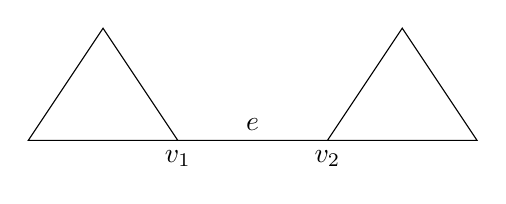
\begin{tikzpicture}[scale=.95]
\draw (2,0) -- (1,1.5) -- (0,0) -- (2,0) node[below] {$v_1$} -- node[above] {$e$} (4,0) node[below] {$v_2$} -- (6,0) -- (5,1.5) -- (4,0);
\end{tikzpicture}
\caption{Eliminar una arista desconecta el grafo}\label{f.five-disconnected-removing}
\end{center}
\end{minipage}
\hfill
\begin{minipage}{.45\textwidth}
\begin{center}
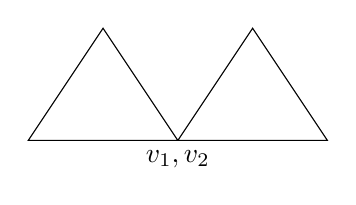
\begin{tikzpicture}[scale=.95]
\draw (2,0) -- (1,1.5) -- (0,0) -- (2,0) node[below] {$v_1,v_2$} -- (4,0) -- (3,1.5) -- (2,0);
\end{tikzpicture}
\caption{Fusión de dos vértices}\label{f.five-disconnected-merge}
\end{center}
\end{minipage}
\end{figure}

\textit{Caso 2:}
El grafo sigue siendo conexo (Fig.~\ref{f.five-connected-remains}). $G'$ tiene menos aristas que $G$ (Fig.~\ref{f.five-connected-fewer}), así que por la hipótesis de inducción $V-(E-1)+(F-1)=2$ ya que al eliminar la arista se unen dos caras en una. Simplificando, obtenemos $V-E+F=2$ para $G$.
\end{proof}

\begin{figure}[ht]
\begin{minipage}{.45\textwidth}
\begin{center}
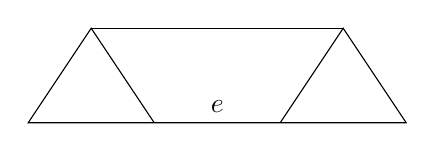
\begin{tikzpicture}[scale=.8]
\draw (2,0) -- (1,1.5) -- (0,0) -- (2,0) -- node[above] {$e$} (4,0) -- (6,0) -- (5,1.5) -- (4,0);
\draw (1,1.5) -- (5,1.5);
\end{tikzpicture}
\caption{Eliminar una arista no desconecta el grafo}\label{f.five-connected-remains}
\end{center}
\end{minipage}
\hfill
\begin{minipage}{.45\textwidth}
\begin{center}
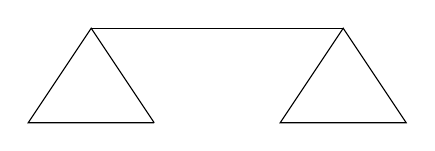
\begin{tikzpicture}[scale=.8]
\draw (2,0) -- (1,1.5) -- (0,0) -- (2,0);
\draw (4,0) -- (5,1.5) -- (6,0) -- cycle;
\draw (1,1.5) -- (5,1.5);
\end{tikzpicture}
\caption{El grafo sigue conectado y tiene menos aristas}\label{f.five-connected-fewer}
\end{center}
\end{minipage}
\end{figure}

\begin{theorem}\label{thm.3v6}
Sea $G$ un grafo plano triangulado conexo con $E$ aristas y $V$ vértices. Entonces $E= 3V-6$.
\end{theorem}
\begin{proof}
Cada cara está limitada por tres aristas, por lo que $E=3F/2$, donde hemos dividido por $2$ porque cada arista se ha contado dos veces, una por cada cara que limita. Por la fórmula de Euler:
\begin{eqnarray*}
E&=&V+F-2\\
&=&V+2E/3-2\\
&=&3V-6\,.
\end{eqnarray*}
\end{proof}

\begin{example}
El grafo plano de la Fig.~\ref{f.five-planar-graph-graph} tiene $10$ vértices y $3\cdot 10-6=24$ aristas.
\end{example}

\begin{theorem}\label{thm.count}
Sea $G$ un grafo plano conexo. Entonces $E\leq 3V-6$.
\end{theorem}

\begin{proof}
Triangulamos $G$ para obtener $G'$. $E'= 3V'-6$ por el Teorema~\ref{thm.3v6}. Ahora quitamos aristas de $G'$ para obtener $G$. El número de vértices no cambia por lo que $E\leq 3V-6$.
\end{proof}

\begin{example}
El grafo de la Fig.~\ref{f.five-fewer} tiene $8$ aristas y $6$ vértices y $8< 3\cdot 6 - 6= 12$.
La figura~\ref{f.five-upper-limit} muestra un grafo triangulado con $6$ vértices y $3\cdot 6 - 6= 12$ aristas.
\end{example}

\begin{figure}[t]
\begin{minipage}{.4\textwidth}
\begin{center}
\begin{tikzpicture}[scale=.8]
\draw (2,0) -- (1,1.5) -- (0,0) -- (2,0) -- (4,0) -- (6,0) -- (5,1.5) -- (4,0);
\draw (1,1.5) -- (5,1.5);
\end{tikzpicture}
\caption{Menos bordes que el límite superior}\label{f.five-fewer}
\end{center}
\end{minipage}
\hfill
\begin{minipage}{.55\textwidth}
\begin{center}
\begin{tikzpicture}[scale=.8]
\draw (2,0) -- (1,1.5) -- (0,0) -- (2,0) -- (4,0) -- (6,0) -- (5,1.5) -- (4,0);
\draw (1,1.5) -- (5,1.5);
\draw (2,0) -- (5,1.5);
\draw (2,0) .. controls (-1,-1) and (-1,1) .. (1,1.5);
\draw (2,0) .. controls (3,-1) .. (6,0) .. controls (7,2) and (4,2) .. (1,1.5);
\end{tikzpicture}
\caption{En un grafo triangulado el número de aristas es máximo}\label{f.five-upper-limit}
\end{center}
\end{minipage}
\end{figure}

%%%%%%%%%%%%%%%%%%%%%%%%%%%%%%%%%%%%%%%%%%%%%%%%%%%%%%%%%%%

\section{Grafos no planos}\label{s.nonplanar}

Vamos a tomar un pequeño desvío para mostrar cómo los Teoremas~\ref{thm.euler} y~\ref{thm.count} se pueden utilizar para demostrar que ciertos grafos no son planos.

\begin{theorem}
$K_5$, el grafo completo de cinco vértices, no es plano (Fig.~\ref{f.five-k5}).
\end{theorem}

\begin{figure}[t]
\begin{minipage}{.48\textwidth}
\begin{center}
\begin{tikzpicture}[scale=.8]
\node (pentagon) [minimum size=4cm,regular polygon,regular polygon sides=5] at (0,0) {};
\draw (pentagon.corner 1) -- (pentagon.corner 2);
\draw (pentagon.corner 2) -- (pentagon.corner 3);
\draw (pentagon.corner 3) -- (pentagon.corner 4);
\draw (pentagon.corner 4) -- (pentagon.corner 5);
\draw (pentagon.corner 5) -- (pentagon.corner 1);
\draw (pentagon.corner 1) -- (pentagon.corner 3);
\draw (pentagon.corner 1) -- (pentagon.corner 4);
\draw (pentagon.corner 2) -- (pentagon.corner 4);
\draw (pentagon.corner 2) -- (pentagon.corner 5);
\draw (pentagon.corner 3) -- (pentagon.corner 5);
\end{tikzpicture}
\caption{$K_5$ no es plano}\label{f.five-k5}
\end{center}
\end{minipage}
\hfill
\begin{minipage}{.5\textwidth}
\begin{center}
\begin{tikzpicture}[scale=.8]
\node (pentagon) [minimum size=4cm,regular polygon,regular polygon sides=5] at (0,0) {};
\draw (pentagon.corner 1) -- (pentagon.corner 2);
\draw (pentagon.corner 2) -- (pentagon.corner 3);
\draw (pentagon.corner 3) -- (pentagon.corner 4);
\draw (pentagon.corner 4) -- (pentagon.corner 5);
\draw (pentagon.corner 5) -- (pentagon.corner 1);
\draw (pentagon.corner 1) .. controls (-4,1) .. 
      (pentagon.corner 3);
\draw (pentagon.corner 1) .. controls (4,1) ..
      (pentagon.corner 4);
\draw (pentagon.corner 2) -- (pentagon.corner 4);
\draw (pentagon.corner 2) -- (pentagon.corner 5);
\draw (pentagon.corner 3) -- (pentagon.corner 5);
\draw[thick] (0,-.95) circle(5pt);
\end{tikzpicture}
\caption{Un intento fallido de dibujar $K_5$ como plano}\label{f.five-k5-failed}
\end{center}
\end{minipage}
\end{figure}

\begin{proof}
Para $K_5$, $V=5$ y $E=10$. Por Teorema~\ref{thm.count} el número de aristas debe ser menor o igual a $3\cdot 5 -6=9$ por lo que el grafo no es plano.
\end{proof}

\begin{theorem}
$K_{3,3}$, el grafo bipartito con tres vértices en cada lado, no es plano (Fig.~\ref{f.five-k33}).
\end{theorem}\index{K33@$K_{3,3}$ is not planar}

\begin{figure}[b]
\begin{minipage}{.45\textwidth}
\begin{center}
\begin{tikzpicture}[scale=.8]
\draw (0,0) -- (3,0);
\draw (0,2) -- (3,2);
\draw (0,4) -- (3,4);
\draw (0,0) -- (3,2);
\draw (0,2) -- (3,4);
\draw (0,4) -- (3,0);
\draw (0,0) -- (3,4);
\draw (0,2) -- (3,0);
\draw (0,4) -- (3,2);
\path (0,-1) -- (3,-1);
\end{tikzpicture}
\caption{$K_{3,3}$ no es plano}\label{f.five-k33}
\end{center}
\end{minipage}
\hfill
\begin{minipage}{.45\textwidth}
\begin{center}
\begin{tikzpicture}[scale=.8]
\draw (0,4) -- (3,4);
\draw (0,2) -- (3,4);
\draw (0,4) .. controls (-1,1) .. (3,0);
\draw (0,0) .. controls (-3,5) .. (3,4);
\draw (0,2) -- (3,0);
\draw (0,4) -- (3,2);

\draw[fill=green] (0,0) -- (3,0) -- (3,0) -- (0,2)  -- (3,2) .. controls (4,-1) .. (0,0);
\draw[thick] (1.5,3) circle(5pt);
\end{tikzpicture}
\caption{Un intento fallido de dibujar $K_{3,3}$ como plano}\label{f.five-k33-failed}
\end{center}
\end{minipage}
\end{figure}

\begin{proof}
$V=6$ y $E=9$. Por Thm~\ref{thm.euler} si $K_{3,3}$ es plano, $F=E-V+2=9-6+2=5$. Pero cada cara está limitada por cuatro aristas (Fig.~\ref{f.five-k33-failed}), por lo que $E=4F/2=10\neq 9$.
\end{proof}

En 1930 Kazimierz Kuratowski demostró la inversa de estos teoremas: si un grafo no es plano, contiene (en cierto sentido) $K_5$ o $K_{3,3}$.

%%%%%%%%%%%%%%%%%%%%%%%%%%%%%%%%%%%%%%%%%%%%%%%%%%%%%%%%%%%

\section{Los grados de los vértices}\label{s.degrees}

\begin{definition}
$d(v)$, el \emph{grado} del vértice $v$, es el número de aristas incidentes a $v$.
\end{definition}\index{Degree of a vertex}

\begin{example}
El grafo de la Fig.~\ref{f.five-planar-graph-graph} contiene $8$ vértices correspondientes a los dos anillos y cada vértice es de grado $5$. El vértice correspondiente a la cara exterior es de grado $4$ al igual que el vértice correspondiente a la cara interior. Por tanto:
\[
\sum_{v\in V} d(v) = 5\cdot 8 + 4\cdot 2=48\,.
\]
Para obtener el número total de aristas dividimos $48$ entre $2$ porque cada arista se ha contado dos veces, una por cada uno de los vértices a los que incide.
\end{example}

Generalizando el argumento obtenemos:
\begin{theorem}\label{thm.degrees}
Sea $d_i$ para $i$ en $\{1,2,3,\ldots,k\}$ el número de vértices de grado $i$ en un grafo plano conexo $G$ con $V$ vértices y $E$ aristas, donde $k$ es el mayor grado de un vértice en $V$. Entonces:
\[
\sum_{v\in V} d(v) =\sum_{i=1}^{k} i\cdot d_i=2E\,.
\]
\end{theorem}

\begin{theorem}\label{thm.degree5}
Sea $G$ un grafo plano conexo con $E$ aristas y $V$ vértices, y sea $d_i$ para $i$ en $\{1,2,3,\ldots,k\}$ el número de vértices de grado $i$, donde $k$ es el mayor grado de un vértice en $V$. Entonces debe haber un vértice $v$ en $V$ tal que $d(v) \leq 5$.
\end{theorem}

\begin{proof}
\mbox{}\\
(1)
Si hay $d_1$ vértices de grado $1$, $d_2$ vértices de grado $2$, \ldots, $d_k$ vértices de grado $k$, entonces $V=\sum_{i=1}^{k}d_i$.  Pos los Teoremas~\ref{thm.count} y \ref{thm.degrees}:
\[
\sum_{i=1}^{k} i\cdot d_i=2E\leq 2(3V-6) = 6V-12=6\sum_{i=1}^{k} d_i -12\,.
\]
Por lo tanto:
\begin{eqnarray*}
\sum_{i=1}^{k} i\cdot d_i &\leq& 6\sum_{i=1}^{k} d_i -12\\
\sum_{i=1}^{k} (6-i)d_i&\geq& 12\,.
\end{eqnarray*}
Como $12>0$ y todos los $d_i$ son positivos, para al menos un $i$, $6-i>0$ y para ese $i$, $i<6$.
\end{proof}

\begin{proof}
\mbox{}\\
(2)
Calculemos el grado promedio de los vértices, que es la suma de los grados dividida por el número de vértices:
\[
d_{\textit{\footnotesize avg}}=\frac{\sum_{i=1}^{k} i\cdot d_i}{V}\,.
\]
Pero la suma de los grados es el doble del número de aristas que por Teorema~\ref{thm.count} da:
\[
d_{\textit{\footnotesize avg}}=\frac{2E}{V}\leq \frac{6V-12}{V}=6-\frac{6}{V}<6\,.
\]
Si el promedio es menor que seis debe haber un vértice de grado menor que seis.
\end{proof}

\begin{example}
En Fig.~\ref{f.five-planar-graph-graph} la suma de los grados es $8\cdot 5 + 2\cdot 4=48$. Hay $10$ vértices por lo que el grado promedio es $48/10=4,8$ y debe haber un vértice de grado $4$ o menos.
\end{example}

%%%%%%%%%%%%%%%%%%%%%%%%%%%%%%%%%%%%%%%%%%%%%%%%%%%%%%%%%%%

\section{El teorema de los seis colores}\label{s.six-color}

\begin{theorem}\label{thm.sixcolor}
Cualquier grafo plano $G$ puede ser coloreado con seis colores.
\end{theorem}\index{Six-color theorem}
\begin{proof}
Por inducción sobre el número de vértices. Si $G$ tiene seis vértices o menos, seis colores son suficientes. Para el paso inductivo, por el Teorema~\ref{thm.degree5} $G$ tiene un vértice $v$ con grado $5$ o menos. Se elimina el vértice $v$ para obtener el grafo $G'$. Por la hipótesis de inducción $G'$ puede ser de seis colores, pero $v$ tiene a lo sumo $5$ vecinos y a lo sumo $5$ colores se utilizan para colorearlos (Fig.~\ref{f.five-six-five}), por el que $v$ se puede colorear utilizando el sexto color (Fig.~\ref{f.five-six-six}).
\end{proof}

\begin{figure}[hbt]
\begin{minipage}{.45\textwidth}
\begin{center}
\begin{tikzpicture}[scale=.5,minimum size=5mm,inner sep=0pt]
\foreach \name/\color/\theta in
    {A/red/18,B/green/90,C/blue!80/162,D/yellow/234,E/orange/306}
  \node[circle,draw,fill=\color] (\name) at (\theta:3) {};
\node[circle,draw] (O) at (0,0) {};
\node[above right] at (O) {$v$};
\foreach \name in {A,B,C,D,E}
  \draw (O) -- (\name);
\foreach \i/\j in {A/B,B/C,D/E}
  \draw (\i) -- (\j);
\draw (B) .. controls (-5,1) .. (D);
\end{tikzpicture}
\caption{Para colorear los vecinos de $v$ cinco colores son suficientes}\label{f.five-six-five}
\end{center}
\end{minipage}
\hfill
\begin{minipage}{.45\textwidth}
\begin{center}
\begin{tikzpicture}[scale=.5,minimum size=5mm,inner sep=0pt]
\foreach \name/\color/\theta in
    {A/red/18,B/green/90,C/blue!80/162,D/yellow/234,E/orange/306}
  \node[circle,draw,fill=\color] (\name) at (\theta:3) {};
\node[circle,draw,fill=brown] (O) at (0,0) {};
\node[above right] at (O) {$v$};
\foreach \name in {A,B,C,D,E}
  \draw (O) -- (\name);
\foreach \i/\j in {A/B,B/C,D/E}
  \draw (\i) -- (\j);
\draw (B) .. controls (-5,1) .. (D);
\end{tikzpicture}
\caption{Coloreamos $v$ con el sexto color}\label{f.five-six-six}
\end{center}
\end{minipage}
\end{figure}

%%%%%%%%%%%%%%%%%%%%%%%%%%%%%%%%%%%%%%%%%%%%%%%%%%%%%%%%%%%

\section{El teorema de los cinco colores}\label{s.five-color}

\begin{definition}
Sea $G$ un grafo planar coloreado. Una cadena \emph{(Kempe)} $G'$ es un subgrafo maximal, bicolor y conexo de $G$.
\end{definition}\index{Kempe chain}

 
\begin{theorem}\label{thm.fivecolor}
Cualquier grafo plano $G$ puede ser coloreado con cinco colores.
\end{theorem}\index{Five-color theorem}

\begin{proof}
Por inducción sobre el número de vértices. Si $G$ tiene cinco vértices o menos, cinco colores son suficientes. Para el paso inductivo, por el Teorema~\ref{thm.degree5}, $G$ tiene un vértice $v$ con grado $5$ o menos. Eliminamos $v$ para obtener $G'$. Por la hipótesis de inducción, $G'$ puede ser oloreado con cinco colores. En $G$, si el grado de $v$ es menor que $5$, o si $v_1,\ldots,v_5$, los vecinos de $v$, están coloreados con cuatro colores o menos, $v$ se puede colorear con el quinto color.
De lo contrario, $v_1,\ldots,v_5$ se colorean con diferentes colores en $G'$ (Fig.~\ref{f.five-color-proof}, arriba).

\begin{figure}
\begin{center}
\begin{tikzpicture}[scale=.48,minimum size=5mm,inner sep=0pt]
\foreach \name/\color/\theta in
    {A/red/18,B/green/90,C/blue!80/162,D/yellow/234,E/orange/306}
  \node[circle,draw,fill=\color] (\name) at (\theta:3) {};
\node[circle,draw] (O) at (0,0) {};
\node[above right] at (O) {$v$};

\node[right,xshift=8pt] at (A) {$v_3$};
\node[right,xshift=8pt] at (B) {$v_2$};
\node[left,,xshift=-8pt] at (C) {$v_1$};
\node[left,,xshift=-8pt] at (D) {$v_5$};
\node[right,xshift=8pt] at (E) {$v_4$};

\foreach \name in {A,B,C,D,E}
  \draw (O) -- (\name);
  
\node[circle,draw,fill=red]  (X1) at (126:5) {};
\node[circle,draw,fill=blue!80] (X2) at (90:7)  {};
\node[circle,draw,fill=red]  (X3) at (36:10) {};
\node[right,xshift=8pt] at (X3) {$v_6$};
\node[circle,draw,fill=blue!80] (X4) at (18:12) {};
\node[right,xshift=8pt] at (X4) {$v_7$};
\node[circle,draw,fill=red]  (X5) at (0:10) {};
\node[circle,draw,fill=blue!80] (X6) at (-18:8) {};
\draw[thick,double distance=2pt] (C)  -- (X1);
\draw[thick,double distance=2pt] (X1) -- (X2);
\draw[thick,double distance=2pt] (X2) -- (X3);
\draw[thick,double distance=2pt] (X3) -- (X4);
\draw[thick,double distance=2pt] (X4) -- (X5);
\draw[thick,double distance=2pt] (X5) -- (X6);
\draw[thick,double distance=2pt] (X6) -- (A);
\draw[thick,double distance=2pt] (A) -- (O) -- (C);

\node[circle,draw,fill=orange]  (Y1)  at (80:5) {};
\node[circle,draw,fill=green]   (Y2)  at (50:7)  {};
\node[circle,draw,fill=orange]  (Y3A) at (20:8) {};
\node[circle,draw,fill=orange]  (Y3B) at (30:5) {};
\node[circle,draw,fill=green]   (Y4A) at (10:6) {};
\node[circle,draw,fill=yellow]  (Y4B) at (10:8) {};
\node[circle,draw,fill=green]   (Y4C) at (15:10) {};
\node[circle,draw,fill=green]   (Y5)  at (-35:7) {};
\node[circle,draw,fill=yellow]  (Y6A) at (-20:12) {};
\node[circle,draw,fill=orange]  (Y6B) at (-20:4) {};
\draw (B)  -- (Y1);
\draw (Y1) -- (Y2);
\draw (Y2) -- (Y3A);
\draw (Y2) -- (Y3B);
\draw (Y3A) -- (Y4A);
\draw (Y3A) -- (Y4B);
\draw (Y3A) -- (Y4C);
\draw (E)  -- (Y5);
\draw (Y5) -- (Y6A);
\draw (Y5) -- (Y6B);
\draw (A) -- (Y1);
\draw (X2) -- (Y1);
\draw (X1) -- (Y1);
\draw (D) -- (E);
\draw (D) -- (C);

\begin{scope}[yshift=-12.85cm]
\foreach \name/\color/\theta in
    {A/red/18,B/green/90,C/blue!80/162,D/yellow/234,E/orange/306}
  \node[circle,draw,fill=\color] (\name) at (\theta:3) {};
\node[circle,draw] (O) at (0,0) {};
\node[above right] at (O) {$v$};

\node[right,xshift=8pt] at (A) {$v_3$};
\node[right,xshift=8pt] at (B) {$v_2$};
\node[left,,xshift=-8pt] at (C) {$v_1$};
\node[left,,xshift=-8pt] at (D) {$v_5$};
\node[right,xshift=8pt] at (E) {$v_4$};

\foreach \name in {A,B,C,D,E}
  \draw (O) -- (\name);
  
\node[circle,draw,fill=red]  (X1) at (126:5) {};
\node[circle,draw,fill=blue!80] (X2) at (90:7)  {};
\node[circle,draw,fill=red]  (X3) at (36:10) {};
\node[circle,draw,fill=blue!80] (X4) at (18:12) {};
\node[circle,draw,fill=red]  (X5) at (0:10) {};
\node[circle,draw,fill=blue!80] (X6) at (-18:8) {};

\draw[thick,double distance=2pt] (C)  -- (X1);
\draw[thick,double distance=2pt] (X1) -- (X2);
\draw[thick,double distance=2pt] (X2) -- (X3);
\draw[thick,double distance=2pt] (X3) -- (X4);
\draw[thick,double distance=2pt] (X4) -- (X5);
\draw[thick,double distance=2pt] (X5) -- (X6);
\draw[thick,double distance=2pt] (X6) -- (A);
\draw[thick,double distance=2pt] (A) -- (O) -- (C);

\node[circle,draw,fill=orange]  (Y1)  at (80:5) {};
\node[circle,draw,fill=green]   (Y2)  at (50:7)  {};
\node[circle,draw,fill=orange]  (Y3A) at (20:8) {};
\node[circle,draw,fill=orange]  (Y3B) at (30:5) {};
\node[circle,draw,fill=green]   (Y4A) at (10:6) {};
\node[circle,draw,fill=yellow]   (Y4B) at (10:8) {};
\node[circle,draw,fill=green]   (Y4C) at (15:10) {};
\node[circle,draw,fill=green]   (Y5)  at (-35:7) {};
\node[circle,draw,fill=yellow]  (Y6A) at (-20:12) {};
\node[circle,draw,fill=orange]  (Y6B) at (-20:4) {};
\draw[thick,dashed,double distance=2pt] (B)  -- (O) -- (E);
\draw[thick,dashed,double distance=2pt] (B)  -- (Y1);
\draw[thick,dashed,double distance=2pt] (Y1) -- (Y2);
\draw[thick,dashed,double distance=2pt] (Y2) -- (Y3A);
\draw[thick,dashed,double distance=2pt] (Y2) -- (Y3B);
\draw[thick,dashed,double distance=2pt] (Y3A) -- (Y4A);
\draw[thick,dashed,double distance=2pt] (Y3A) -- (Y4B);
\draw[thick,dashed,double distance=2pt] (Y3A) -- (Y4C);
\draw[thick,dashed,double distance=2pt] (E)  -- (Y5);
\draw[thick,dashed,double distance=2pt] (Y5) -- (Y6B);
\draw (Y5) -- (Y6A);
\draw (A) -- (Y1);
\draw (X2) -- (Y1);
\draw (X1) -- (Y1);
\draw (D) -- (E);
\draw (D) -- (C);
\node[right,xshift=8pt] at (X3) {$v_6$};
\node[right,xshift=8pt] at (X4) {$v_7$};
\end{scope}

\begin{scope}[yshift=-25.7cm]
\foreach \name/\color/\theta in
    {A/red/18,B/orange/90,C/blue!80/162,D/yellow/234,E/orange/306}
  \node[circle,draw,fill=\color] (\name) at (\theta:3) {};
\node[circle,draw,fill=green] (O) at (0,0) {};
\node[above right] at (O) {$v$};

\node[right,xshift=8pt] at (A) {$v_3$};
\node[right,xshift=8pt] at (B) {$v_2$};
\node[left,,xshift=-8pt] at (C) {$v_1$};
\node[left,,xshift=-8pt] at (D) {$v_5$};
\node[right,xshift=8pt] at (E) {$v_4$};

\foreach \name in {A,B,C,D,E}
  \draw (O) -- (\name);
  
\node[circle,draw,fill=red]  (X1) at (126:5) {};
\node[circle,draw,fill=blue!80] (X2) at (90:7)  {};
\node[circle,draw,fill=red]  (X3) at (36:10) {};
\node[circle,draw,fill=blue!80] (X4) at (18:12) {};
\node[circle,draw,fill=red]  (X5) at (0:10) {};
\node[circle,draw,fill=blue!80] (X6) at (-18:8) {};

\draw[thick,double distance=2pt] (C)  -- (X1);
\draw[thick,double distance=2pt] (X1) -- (X2);
\draw[thick,double distance=2pt] (X2) -- (X3);
\draw[thick,double distance=2pt] (X3) -- (X4);
\draw[thick,double distance=2pt] (X4) -- (X5);
\draw[thick,double distance=2pt] (X5) -- (X6);
\draw[thick,double distance=2pt] (X6) -- (A);
\draw[thick,double distance=2pt] (A) -- (O) -- (C);

\node[circle,draw,fill=green]  (Y1)  at (80:5) {};
\node[circle,draw,fill=orange]   (Y2)  at (50:7)  {};
\node[circle,draw,fill=green]  (Y3A) at (20:8) {};
\node[circle,draw,fill=green]  (Y3B) at (30:5) {};
\node[circle,draw,fill=orange]   (Y4A) at (10:6) {};
\node[circle,draw,fill=yellow]   (Y4B) at (10:8) {};
\node[circle,draw,fill=orange]   (Y4C) at (15:10) {};
\node[circle,draw,fill=green]   (Y5)  at (-35:7) {};
\node[circle,draw,fill=yellow]  (Y6A) at (-20:12) {};
\node[circle,draw,fill=orange]  (Y6B) at (-20:4) {};

\draw[thick,dashed,double distance=2pt] (B)  -- (O) -- (E);
\draw[thick,dashed,double distance=2pt] (B)  -- (Y1);
\draw[thick,dashed,double distance=2pt] (Y1) -- (Y2);
\draw[thick,dashed,double distance=2pt] (Y2) -- (Y3A);
\draw[thick,dashed,double distance=2pt] (Y2) -- (Y3B);
\draw[thick,dashed,double distance=2pt] (Y3A) -- (Y4A);
\draw[thick,dashed,double distance=2pt] (Y3A) -- (Y4B);
\draw[thick,dashed,double distance=2pt] (Y3A) -- (Y4C);
\draw[thick,dashed,double distance=2pt] (E)  -- (Y5);
\draw[thick,dashed,double distance=2pt] (Y5) -- (Y6B);


\draw (Y5) -- (Y6A);
\draw (A) -- (Y1);
\draw (X2) -- (Y1);
\draw (X1) -- (Y1);
\draw (D) -- (E);
\draw (D) -- (C);
\node[right,xshift=8pt] at (X3) {$v_6$};
\node[right,xshift=8pt] at (X4) {$v_7$};
\end{scope}
\end{tikzpicture}
\end{center}
\caption{Demostración del teorema de los cinco colores}\label{f.five-color-proof}
\end{figure}

Consideremos el vértice $v_1$ que es de color azul y el vértice $v_3$ que es de color rojo. Si $v_1,v_3$ no están conectados por un camino azul-rojo (digamos si la arista $\overline{v_6v_7}$ no existiera), podemos intercambiar los colores a lo largo del camino de $v_1$ a $v_6$ y colorear $v$ de azul. De lo contrario, consideremos la cadena azul-rojo que contiene $v_1,v_3$. Sumando $v$ y las aristas $\overline{vv_1},\overline{vv_3}$ obtenemos un camino cerrado $P$ (línea doble) que divide el plano en una región ``interior'' y otra ``exterior'' (Fig~\ref{f.five-color-proof}, centro).

Consideremos $v_2$ que es de color verde y $v_4$ que es de color naranja. Estos vértices no pueden estar contenidos en una sola cadena verde-naranja, porque $v_2$ está dentro de $P$ y $v_4$ está fuera de $P$, por lo que cualquier camino que los conecte debe cruzar $P$, contradiciendo la suposición de que el grafo es plano. Por lo tanto, deben estar contenidas en dos cadenas verde-naranja (doble línea discontinua, en la Fig.~\ref{f.five-color-proof}, centro).
Intercambiamos los colores en la cadena que contiene $v_2$ y luego $v$ puede ser de color verde para obtener una coloración de G con cinco colores de $G$ (Fig.~\ref{f.five-color-proof}, abajo).
\end{proof}

\begin{advanced}
La afirmación de que un camino continuo desde el interior de una curva continua cerrada $P$ al exterior de $P$ debe intersecar a $P$ es el Teorema de la Curva de Jordan. El teorema es intuitivamente obvio, pero difícil de demostrar.
\end{advanced}

%%%%%%%%%%%%%%%%%%%%%%%%%%%%%%%%%%%%%%%%%%%%%%%%%%%%%%%%%%%

\section{Demostración incorrecta del teorema de los cuatro colores de Kempe}\label{s.kempe}

\begin{theorem}\label{thm.fourcolor}
Todo grafo plano puede ser coloraedo con cuatro colores.
\end{theorem}\index{Four-color theorem}

\begin{proof} (Incorrecta) El caso base de la inducción y la mayor parte de la demostración es son los mismos que los del teorema de los cinco colores. El nuevo caso que hay que considerar es un vértice $v$ con cinco vecinos que, por la hipótesis inductiva, se puede colorear con cuatro colores después de quitar $v$.

En la Fig.~\ref{f.five-kempe1} hay dos vértices $v_2,v_5$ coloreados de azul. Consideremos la cadena azul-verde que contiene $v_2$ y la cadena azul-amarilla que contiene $v_5$. La cadena azul-verde está contenida dentro de la trayectoria cerrada definida por la cadena rojo-amarilla que contiene $v_1,v_3$ (línea doble) y la cadena azul-amarilla está contenida dentro de la trayectoria cerrada definida por la cadena rojo-verde que contiene $v_1,v_4$ (línea doble discontinua).

Intercambiamos los colores de la cadena azul-verde y la cadena azul-amarillo (Fig.~\ref{f.five-kempe1-exchange}). El resultado es que los vecinos de $v$ se colorean con los tres colores rojo, verde y amarillo, dejando libre el azul para colorear $v$.
\end{proof}

\begin{figure}[ht]
\begin{minipage}{.45\textwidth}
\begin{center}
\begin{tikzpicture}[scale=.5,minimum size=5mm,inner sep=0pt]

% Draw center node and adjacent nodes
\foreach \name/\color/\theta in
    {A/yellow/18,B/blue!80/90,C/red/162,D/blue!80/234,E/green/306}
  \node[circle,draw,fill=\color] (\name) at (\theta:3) {};
\node[circle,draw] (O) at (0,0) {};
\node[above right]     at (O) {$v$};

\node[right,xshift=10pt] at (A) {$v_3$};
\node[left,xshift=-8pt]  at (B) {$v_2$};
\node[left,xshift=-8pt]  at (C) {$v_1$};
\node[left,xshift=-8pt]  at (D) {$v_5$};
\node[right,xshift=8pt]  at (E) {$v_4$};

% Draw red-yellow path
\node[circle,draw,fill=yellow]  (X1) at (126:5) {};
\node[circle,draw,fill=red] (X2) at (45:8)  {};

\draw[thick,double distance=2pt] 
  (C) -- (X1) -- (X2) -- (A) -- (O);
\draw[thick,double distance=6pt] (O) -- (C);

% Draw blue-green nodes within red-yellow path
\node[circle,draw,fill=green] (Y1)  at (50:5) {};

% Draw red-green path
\node[circle,draw,fill=green] (Z1)  at (-160:5) {};
\node[circle,draw,fill=red]   (Z2)  at (-80:6)  {};

\draw[thick,dashed,double distance=2pt] 
  (O) -- (C) -- (Z1) -- (Z2) -- (E) -- (O);

% Draw blue-yellow nodes within red-green path
\node[circle,draw,fill=yellow]   (U1)  at (-90:4)  {};

% Connect adjacent nodes not in paths
\draw (X1) -- (B) -- (Y1) -- (A) -- (B) -- 
      (C) -- (D) -- (E) -- (A);
\draw (Z2) -- (U1) -- (D) -- (O) -- (B);
\node[above,yshift=8pt] at (X1) {$v_6$};
\node[below,yshift=-8pt] at (Z1) {$v_7$};
\node[left,xshift=-8pt] at (Z2) {$v_8$};
\end{tikzpicture}
\caption{Cadenas Kempe azul-verde y azul-amarillo}\label{f.five-kempe1}
\end{center}
\end{minipage}
\hfill
\begin{minipage}{.45\textwidth}
\begin{center}
\begin{tikzpicture}[scale=.5,minimum size=5mm,inner sep=0pt]

% Draw center node and adjacent nodes
\foreach \name/\color/\theta in
    {A/yellow/18,B/green/90,C/red/162,D/yellow/234,E/green/306}
  \node[circle,draw,fill=\color] (\name) at (\theta:3) {};
\node[circle,draw,fill=blue!80] (O) at (0,0) {};
\node[above right]     at (O) {$v$};

\node[right,xshift=10pt] at (A) {$v_3$};
\node[left,xshift=-8pt]  at (B) {$v_2$};
\node[left,xshift=-8pt]  at (C) {$v_1$};
\node[left,xshift=-8pt]  at (D) {$v_5$};
\node[right,xshift=8pt]  at (E) {$v_4$};

% Draw red-yellow path
\node[circle,draw,fill=yellow]  (X1) at (126:5) {};
\node[circle,draw,fill=red] (X2) at (45:8)  {};

\draw[thick,double distance=2pt] 
  (C) -- (X1) -- (X2) -- (A) -- (O);
\draw[thick,double distance=6pt] (O) -- (C);

% Draw blue-green nodes within red-yellow path
\node[circle,draw,fill=blue!80] (Y1)  at (50:5) {};

% Draw red-green path
\node[circle,draw,fill=green] (Z1)  at (-160:5) {};
\node[circle,draw,fill=red]   (Z2)  at (-80:6)  {};

\draw[thick,dashed,double distance=2pt] 
  (O) -- (C) -- (Z1) -- (Z2) -- (E) -- (O);

% Draw blue-yellow nodes within red-green path
\node[circle,draw,fill=blue!80]   (U1)  at (-90:4)  {};

% Connect adjacent nodes not in paths
\draw (X1) -- (B) -- (Y1) -- (A) -- (B) -- 
      (C) -- (D) -- (E) -- (A);
\draw (Z2) -- (U1) -- (D) -- (O) -- (B);
\node[above,yshift=8pt] at (X1) {$v_6$};
\node[below,yshift=-8pt] at (Z1) {$v_7$};
\node[left,xshift=-8pt] at (Z2) {$v_8$};
\end{tikzpicture}
\caption{Intercambia los colores de las dos cadenas Kempe}\label{f.five-kempe1-exchange}
\end{center}
\end{minipage}
\end{figure}

Heawood observó que los caminos cerrados definidos por la cadena rojo-amarillo y la cadena rojo-verde pueden compartir vértices rojos ($v_1,v_8$ en Fig.~\ref{f.five-kempe2}). Cuando se intercambian los colores en las cadenas azul-verde y azul-amarillo, es posible que los vértices azules $v_6,v_7$ estén conectados (Fig.~\ref{f.five-kempe2-share}) y la coloración ya no es correcta.

\begin{figure}[ht]
\begin{minipage}{.50\textwidth}
\begin{center}
\begin{tikzpicture}[scale=.5,minimum size=5mm,inner sep=0pt]

% Draw center node and adjacent nodes
\foreach \name/\color/\theta in
    {A/yellow/18,B/blue!80/90,C/red/162,D/blue!80/234,E/green/306}
  \node[circle,draw,fill=\color] (\name) at (\theta:3) {};
\node[circle,draw] (O) at (0,0) {};
\node[above right]     at (O) {$v$};

\node[right,xshift=10pt] at (A) {$v_3$};
\node[right,xshift=8pt]  at (B) {$v_2$};
\node[above right,xshift=8pt]  at (C) {$v_1$};
\node[below right,yshift=-8pt] at (D) {$v_5$};
\node[right,xshift=8pt]  at (E) {$v_4$};

% Draw red-yellow path
\node[circle,draw,fill=yellow] (X1) at (-170:5) {};
\node[circle,draw,fill=red]    (X2) at (-80:7)  {};

\draw[thick,double distance=2pt] (A) -- (O);
\draw[thick,double distance=6pt] (O) -- (C);
\draw[thick,double distance=2pt] (C) --(X1) -- (X2);
\draw[thick,double distance=2pt,bend right=40] (X2) to (A);

% Draw red-green path
\node[circle,draw,fill=green] (Y1) at (100:6)  {};

\draw[dashed,thick,double distance=2pt] (O) -- (C) -- (Y1);
\draw[dashed,thick,double distance=2pt] 
  (Y1) .. controls (40:10) and (-50:9) .. (X2);
\draw[dashed,thick,double distance=2pt] (X2) -- (E) -- (O);

% Draw adjacent nodes
\draw (X1) -- (D) -- (O) -- (B) -- (Y1) -- (X1);
\node[left,xshift=-8pt] at (Y1) {$v_6$};
\node[below,yshift=-8pt] at (X1) {$v_7$};
\node[left,xshift=-8pt] at (X2) {$v_8$};
\end{tikzpicture}
\caption{Las cadenas rojo-amarillo\\y rojo-verde comparten vértices rojos}\label{f.five-kempe2}
\end{center}
\end{minipage}
\hfill
\begin{minipage}{.50\textwidth}
\begin{center}
\begin{tikzpicture}[scale=.5,minimum size=5mm,inner sep=0pt]

% Draw center node and adjacent nodes
\foreach \name/\color/\theta in
    {A/yellow/18,B/green/90,C/red/162,D/yellow/234,E/green/306}
  \node[circle,draw,fill=\color] (\name) at (\theta:3) {};
\node[circle,draw,fill=blue!80] (O) at (0,0) {};
\node[above right]     at (O) {$v$};

\node[right,xshift=10pt] at (A) {$v_3$};
\node[right,xshift=8pt]  at (B) {$v_2$};
\node[above right,xshift=8pt]  at (C) {$v_1$};
\node[below right,yshift=-8pt] at (D) {$v_5$};
\node[right,xshift=8pt]  at (E) {$v_4$};

% Draw red-yellow path
\node[circle,draw,fill=blue!80] (X1) at (-170:5) {};
\node[circle,draw,fill=red]  (X2) at (-80:7)  {};

\draw[thick,double distance=2pt] (A) -- (O);
\draw[thick,double distance=6pt] (O) -- (C);
\draw[thick,double distance=2pt] (C) --(X1) -- (X2);
\draw[thick,double distance=2pt,bend right=40] (X2) to (A);

% Draw red-green path
\node[circle,draw,fill=blue!80] (Y1) at (100:6)  {};

\draw[dashed,thick,double distance=2pt] (O) -- (C) -- (Y1);
\draw[dashed,thick,double distance=2pt] 
  (Y1) .. controls (40:10) and (-50:9) .. (X2);
\draw[dashed,thick,double distance=2pt] (X2) -- (E) -- (O);

% Draw adjacent nodes
\draw (X1) -- (D) -- (O) -- (B) -- (Y1) -- (X1);
\node[left,xshift=-8pt] at (Y1) {$v_6$};
\node[below,yshift=-8pt] at (X1) {$v_7$};
\node[left,xshift=-8pt] at (X2) {$v_8$};
\end{tikzpicture}
\caption{El intercambio de colores hace que los vértices azules se conecten}\label{f.five-kempe2-share}
\end{center}
\end{minipage}
\end{figure}

\subsection*{¿Cuál es la sorpresa?}

El teorema de los cuatro colores es famoso porque es muy fácil de enunciar pero extremadamente difícil de demostrar. Por lo tanto, es sorprendente que la demostración del teorema de los cinco colores sea elemental. La parte inteligente de la demostración es el Teorema~\ref{thm.degree5} (un grafo plano debe tener un vértice de como máximo grado $5$), que es un teorema que no tiene nada que ver con la coloración. Simplemente, resulta simplemente de contar vértices y aristas.

\subsection*{Fuentes}

Para el teorema de los cuatro colores, véase \cite{thomas,wiki:four}. La demostración del teorema de los cinco colores se basa en \cite{thebook,wiki:five}.
\cite{eppstein} presenta numerosas demostraciones de la fórmula de Euler. La demostración incorrecta de Kempe del teorema de los cuatro colores se describe en \cite{sipka}.


\tikzsetfigurename{museum}
% !TeX root = surprises.tex

\selectlanguage{hebrew}



\chapter{איך לשמור על מוזיאון}
\label{c.museum}

ב-%
$1973$
\L{Victor Klee}
שאל כמה שומרים נחוצים כדי לראות את כל הקירות של מוזיאון על מנת לוודא שלא גונבים את הציורים. אם הקירות של המוזיאון מהווים מצולע משוכלל או אפילו מצולע קמור, אפשר להסתפק בשומר אחד:
\begin{center}

\begin{tikzpicture}[scale=.8]
\coordinate (O) at (0,0);
\fill (O) circle (2pt);
\foreach \x/\name/\n/\po in {0/a/A/right,.6/b/B/above,1.6/c/C/left,2.4/d/D/below left,3.9/e/E/below right} {
  \coordinate (\name) at ($(O)+(\x*72+18:3cm)$);
%  \fill (\name) circle (1.5pt);
%  \node[\po] at (\name) {$\n$};
\draw[dashed] (O) -- (\name);
}
\draw (a) -- (b) -- (c) -- (d) --(e) -- cycle;
\end{tikzpicture}
\end{center}

מה עם מוזיאון עם קירות בצורה של מסור:

\begin{center}

\begin{tikzpicture}[scale=1]
\coordinate (O) at (0,0);
\draw [thick] (O) -- (++110:1cm) coordinate (P);
\draw[thick] (O) --
  ++(-70:1cm) coordinate(A) node[below] {$1$} -- 
  ++(+70:1cm) -- ++(0:1.5cm) --
  ++(-70:1cm) coordinate(B) node[below] {$2$} -- 
  ++(+70:1cm) -- ++(0:1.5cm) --
  ++(-70:1cm) coordinate(C) node[below] {$3$}-- 
  ++(+70:1cm) -- ++(0:1.5cm) --
  ++(-70:1cm) coordinate(D) node[below] {$4$} -- 
  ++(+70:1cm) -- ++(0:1.5cm) --
  ++(-70:1cm) coordinate(E) node[below] {$5$} --
  ++(+70:2cm) -- (P);

\end{tikzpicture}
\end{center}

וודא על ידי ספירה שיש 
$15$
קירות.

כל "שן" של המסור מגדירה משולש )מסומן באפור(. שומרת הניצבת במקום כלשהו בתוך אחד המשולשים יכולה לראות את כל הקירות של אותו משולש:

\begin{center}

\begin{tikzpicture}[scale=1]
\coordinate (O) at (0,0);
\draw [thick] (O) -- (++110:1cm) coordinate (P);
\draw[thick] (O) --
  ++(-70:1cm) coordinate(A) node[below] {$1$} -- 
  ++(+70:1cm) -- ++(0:1.5cm) --
  ++(-70:1cm) coordinate(B) node[below] {$2$} -- 
  ++(+70:1cm) -- ++(0:1.5cm) --
  ++(-70:1cm) coordinate(C) node[below] {$3$}-- 
  ++(+70:1cm) -- ++(0:1.5cm) --
  ++(-70:1cm) coordinate(D) node[below] {$4$} -- 
  ++(+70:1cm) -- ++(0:1.5cm) --
  ++(-70:1cm) coordinate(E) node[below] {$5$} --
  ++(+70:2cm) -- (P);

\draw[fill,black!20!white] (A) -- ++(110:2cm) -- ++(0:1.35cm)-- cycle;
\draw[fill,black!20!white] (B) -- ++(110:2cm) -- ++(0:1.35cm)-- cycle;
\draw[fill,black!20!white] (C) -- ++(110:2cm) -- ++(0:1.35cm)-- cycle;
\draw[fill,black!20!white] (D) -- ++(110:2cm) -- ++(0:1.35cm)-- cycle;
\draw[fill,black!20!white] (E) -- ++(110:2cm) -- ++(0:1.35cm)-- cycle;

\draw[->,red,very thick] (2.7,.8) -- +(-100:1.5cm);
\draw[->,red,very thick] (6.4,.6) -- +(-55:1.2cm);
%\draw[->,very thick,green] (9,.9) -- (C);
%\draw[->,very thick,blue] ($(O)+(.5,.5)$) -- ++(7.5,.42);
%\draw[->,very thick,blue] ($(O)+(.5,.5)$) -- ++(3,-.5);
\end{tikzpicture}
\end{center}

אם השומרת ניצבת בקירבת הקיר העליון היא יכולה לראות את כל הקירות האופקיים )חצים כחולים(. ברור שחמש
שומרות מספיקות כדי לשמור על כל הקירות. אם המשולשים לא חופפים, שומרת במשולש אחד לא יכולה לראות את כל הקירות של משולש אחר )חץ ירוק(, לכן חייבים להעסיק חמש שומרות נחוצות.

\begin{center}

\begin{tikzpicture}[scale=1]
\coordinate (O) at (0,0);
\draw [thick] (O) -- (++110:1cm) coordinate (P);
\draw[thick] (O) --
  ++(-70:1cm) coordinate(A) node[below] {$1$} -- 
  ++(+70:1cm) -- ++(0:1.5cm) --
  ++(-70:1cm) coordinate(B) node[below] {$2$} -- 
  ++(+70:1cm) -- ++(0:1.5cm) --
  ++(-70:1cm) coordinate(C) node[below] {$3$}-- 
  ++(+70:1cm) -- ++(0:1.5cm) --
  ++(-70:1cm) coordinate(D) node[below] {$4$} -- 
  ++(+70:1cm) -- ++(0:1.5cm) --
  ++(-70:1cm) coordinate(E) node[below] {$5$} --
  ++(+70:2cm) -- (P);

\draw[fill,black!20!white] (A) -- ++(110:2cm) -- ++(0:1.35cm)-- cycle;
\draw[fill,black!20!white] (B) -- ++(110:2cm) -- ++(0:1.35cm)-- cycle;
\draw[fill,black!20!white] (C) -- ++(110:2cm) -- ++(0:1.35cm)-- cycle;
\draw[fill,black!20!white] (D) -- ++(110:2cm) -- ++(0:1.35cm)-- cycle;
\draw[fill,black!20!white] (E) -- ++(110:2cm) -- ++(0:1.35cm)-- cycle;

%\draw[->,red,very thick] (2.7,1) -- (B);
\draw[->,very thick,green,dashed] (9,.8) -- +(-165:4.6cm);
\draw[->,very thick,blue] ($(O)+(.5,.5)$) -- ++(7.4,.4);
\draw[->,very thick,blue] ($(O)+(.5,.5)$) -- ++(2.9,-.45);
\draw (6,0) circle(4pt);
\draw (4.95,-.28) circle(4pt);
\end{tikzpicture}
\end{center}
\begin{theorem}\label{thm.guarded} \mbox{}\\
$\disfrac{n}{3}$
שומרות מספיקות ונחוצות כדי לשמור על כל מוזיאון עם
$n$
קירות.%
\footnote{\R{אם}
$n$
\R{לא מתחלק ב}-%
$3$
\R{מספר השומרות הנחוצות הוא}
$\left\lfloor \disfrac{n}{3}\right\rfloor$.
\R{למשל,}
$4$
\R{שומרות מספיקות כדי לשמור על מוזיאונים עם}
$12, 13, 14$
\R{קירות כי}
$\left\lfloor \disfrac{14}{3}\right\rfloor =\left\lfloor \disfrac{13}{3}\right\rfloor=\left\lfloor \disfrac{12}{3}\right\rfloor=4$.
\R{לשם הפשטות נתעלם מסיבוך זה}.}
\end{theorem}
ניתן להכליל את הדוגמה כדי להראות ש-%
$\disfrac{n}{3}$
שומרות נחוצות. שאר הפרק מוקדש להוכחה ש-%
$\disfrac{n}{3}$
מספיקות עבור כל מוזיאון.

\section{צביעת מצולעים מתולתים}

\textbf{הגדרה:}
קודקוד במצולע הוא 
\textbf{קמור}
אם הזווית הפנימית פחות מ-%
$180^\circ$.
קודקוד במצולע הוא
\textbf{קעור}
אם הזווית הפנימית גדולה מ-%
$180^\circ$.

במצולע באיור להלן, קודקוד 
$1$
קמור וקודקוד
$2$
קעור.
\begin{center}

\begin{tikzpicture}[scale=.8]
\draw[thick]
  (0,0) coordinate (A) node[below left] {$1$} -- 
  ++(3,0) coordinate (B) --
  ++(2,2) coordinate (C) --
  ++(-1.5,-.5) coordinate (D) --
  ++(3,3) coordinate (E) -- 
  ++(-4,-1) coordinate (F) --
  ++(-2,1) coordinate (G) --
  ++(-1,-1) coordinate (H) --
  ++(.5,-1.5) coordinate (I) --
  ++(-2,-.5) coordinate (J) --
  ++(3,-.2) coordinate (K) node[right] {$2$} -- 
  ++(-4,-.3) coordinate (L) --
  cycle;
  
\foreach \point in {A,B,C,D,E,F,G,H,I,J,K,L}
  \fill (\point) circle(1.25pt);
\end{tikzpicture}
\end{center}
\textbf{הגדרה:}
ניתן
\textbf{לתלת}
\L{(triangulate)}
מצולע אם ניתן לצייר 
\textbf{אלכסונים},
קטעי קו שאינם נחתכים המחברים קודקודים והנמצאים בתוך המצולע לכל אורכם, כך שהשטח הפנימי של המצולע מכוסה על ידי משולשים זרים אחד מהשני.



\begin{theorem}\label{thm.tri}\mbox{}\\
ניתן לתלת כל מצולע.
\end{theorem}
אנו דוחים את ההוכחה של משפט~%
\ref{thm.tri}
לשלב מאוחר יותר.
\textbf{הגדרה:}
ניתן
\textbf{לצבוע מצולע בשלושה צבעים}
אם קיים מיפוי
\[
c: V \mapsto \{\textrm{\R{אדום, כחול, ירוק}}\}
\]
כך ששני הקודקודים של צלע מקבלים צבעים שונים.
\begin{theorem}\mbox{}\\
ניתן לצבוע מצולע מתולת בשלושה צבעים.
\label{thm.colored}
\end{theorem}
\textbf{הוכחה:}
באינדוקציה על מספר הקודקודים. ברור שניתן לצבוע משולש בשלושה צבעים. ניתן מצולע עם 
$n>3$
קודקודים. חייבים לצייר לפחות אלכסון אחד כדי לתלת את המצולע. בחר אלכסון שרירותי
$\overline{AB}$:

\begin{center}

\begin{tikzpicture}[scale=.8]
\draw[thick]
  (0,0) coordinate (A) -- 
  ++(3,0) coordinate (B) --
  ++(2,2) coordinate (C) --
  ++(-1.5,-.5) coordinate (D) --
  ++(3,3) coordinate (E) -- 
  ++(-4,-1) coordinate (F) --
  ++(-2,1) coordinate (G) --
  ++(-1,-1) coordinate (H) --
  ++(.5,-1.5) coordinate (I) --
  ++(-2,-.5) coordinate (J) --
  ++(3,-.2) coordinate (K) -- 
  ++(-4,-.3) coordinate (L) --
  cycle;
  
\foreach \point in {A,B,C,D,E,F,G,H,I,J,K,L}
  \fill (\point) circle(1.25pt);

\node[above right,xshift=4pt] at (K) {$A$};
\node[above left,xshift=-4pt,yshift=-2pt] at (D) {$B$};

\draw[thick,dashed]
  (B) -- (D) -- (K) -- (F) -- (I) -- (K) -- (A) -- (D) -- (F) -- (H);
\end{tikzpicture}
\end{center}
וחלק את המצולע לאורך אלכסון זה לשני מצולעים קטנים יותר:
\begin{center}

\begin{tikzpicture}[scale=.8]
\path
  (0,0) coordinate (A1) -- 
  ++(3,0) coordinate (B1) --
  ++(2,2) coordinate (C1) --
  ++(-1.5,-.5) coordinate (D1);
\draw[thick]
  (D1) --
  ++(3,3) coordinate (E1) -- 
  ++(-4,-1) coordinate (F1) --
  ++(-2,1) coordinate (G1) --
  ++(-1,-1) coordinate (H1) --
  ++(.5,-1.5) coordinate (I1) --
  ++(-2,-.5) coordinate (J1) --
  ++(3,-.2) coordinate (K1);
\path
  (K1) -- 
  ++(-4,-.3) coordinate (L1) --
  (A1);
  
\foreach \point in {D1,E1,F1,G1,H1,I1,J1,K1}
  \fill (\point) circle(1.25pt);

\node[below,yshift=-4pt] at (K1) {$A$};
\node[below,yshift=-4pt] at (D1) {$B$};

\draw[thick,dashed]
  (D1) -- (F1) -- (I1) -- (K1) -- (F1) -- (H1);
\draw[thick] (D1) -- (K1);

\begin{scope}[yshift=-1.8cm]

\draw[thick]
  (0,0) coordinate (A2) -- 
  ++(3,0) coordinate (B2) --
  ++(2,2) coordinate (C2) --
  ++(-1.5,-.5) coordinate (D2);
\path
  (D2) --
  ++(3,3) coordinate (E2) --
  ++(-4,-1) coordinate (F2) --
  ++(-2,1) coordinate (G2) --
  ++(-1,-1) coordinate (H2) --
  ++(.5,-1.5) coordinate (I2) --
  ++(-2,-.5) coordinate (J2) --
  ++(3,-.2) coordinate (K2);
\draw[thick]
  (K2) --
  ++(-4,-.3) coordinate (L2) --
  (A2);
  
\foreach \point in {A2,B2,C2,D2,K2,L2}
  \fill (\point) circle(1.25pt);
  
\node[above,yshift=4pt] at (K2) {$A$};
\node[above,yshift=4pt] at (D2) {$B$};

\draw[thick,dashed]
  (K2) -- (A2) -- (D2) -- (B2) -- (D2);
\draw[thick] (D2) -- (K2);

\end{scope}
\end{tikzpicture}
\end{center}
לפי הנחת האינדוקציה, ניתן לצבוע כל אחד מהמצולעים הללו בשלושה צבעים:
\begin{center}

\begin{tikzpicture}[scale=.8]
\path
  (0,0) coordinate (A1) -- 
  ++(3,0) coordinate (B1) --
  ++(2,2) coordinate (C1) --
  ++(-1.5,-.5) coordinate (D1);
\draw[thick]
  (D1) --
  ++(3,3) coordinate (E1) -- 
  ++(-4,-1) coordinate (F1) --
  ++(-2,1) coordinate (G1) --
  ++(-1,-1) coordinate (H1) --
  ++(.5,-1.5) coordinate (I1) --
  ++(-2,-.5) coordinate (J1) --
  ++(3,-.2) coordinate (K1);
\path
  (K1) -- 
  ++(-4,-.3) coordinate (L1) --
  (A1);
  
\draw[thick,dashed]
  (D1) -- (F1) -- (I1) -- (K1) -- (F1) -- (H1);
\draw[thick] (D1) -- (K1);

\node[below,yshift=-4pt] at (K1) {$A$};
\node[below,yshift=-4pt] at (D1) {$B$};

\foreach \point/\color in {D1/red,E1/blue,F1/green,G1/red,H1/blue,I1/red,J1/green,K1/blue}
  \fill[color=\color] (\point) circle(5pt);


\begin{scope}[yshift=-1.8cm]

\draw[thick]
  (0,0) coordinate (A2) -- 
  ++(3,0) coordinate (B2) --
  ++(2,2) coordinate (C2) --
  ++(-1.5,-.5) coordinate (D2);
\path
  (D2) --
  ++(3,3) coordinate (E2) --
  ++(-4,-1) coordinate (F2) --
  ++(-2,1) coordinate (G2) --
  ++(-1,-1) coordinate (H2) --
  ++(.5,-1.5) coordinate (I2) --
  ++(-2,-.5) coordinate (J2) --
  ++(3,-.2) coordinate (K2);
\draw[thick]
  (K2) --
  ++(-4,-.3) coordinate (L2) --
  (A2);
  
\draw[thick,dashed]
  (K2) -- (A2) -- (D2) -- (B2) -- (D2);
\draw[thick] (D2) -- (K2);
\node[above,yshift=4pt] at (K2) {$A$};
\node[above,yshift=4pt] at (D2) {$B$};

\foreach \point/\color in {A2/red,B2/blue,C2/red,D2/green,K2/blue,L2/green}
  \fill[color=\color] (\point) circle(5pt);


\end{scope}
\end{tikzpicture}
\end{center}
השיוך של צבעים לקודקודים הוא שרירותי, כך שאם הקודקודים 
$A,B$
מקבלים צבעים שונים בשני המצולעים, ניתן לשנות את הצבעים באחד מהם כך שהצבעים של 
$A,B$
זהים בשני המצולעים. נחליף את הצבעים
\textbf{אדום}
ו-%
\textbf{ירוק}
במצולע התחתון:
\begin{center}

\begin{tikzpicture}[scale=.8]
\path
  (0,0) coordinate (A1) -- 
  ++(3,0) coordinate (B1) --
  ++(2,2) coordinate (C1) --
  ++(-1.5,-.5) coordinate (D1);
\draw[thick]
  (D1) --
  ++(3,3) coordinate (E1) -- 
  ++(-4,-1) coordinate (F1) --
  ++(-2,1) coordinate (G1) --
  ++(-1,-1) coordinate (H1) --
  ++(.5,-1.5) coordinate (I1) --
  ++(-2,-.5) coordinate (J1) --
  ++(3,-.2) coordinate (K1);
\path
  (K1) -- 
  ++(-4,-.3) coordinate (L1) --
  (A1);
  
\node[below,yshift=-4pt] at (K1) {$A$};
\node[below,yshift=-4pt] at (D1) {$B$};

\draw[thick,dashed]
  (D1) -- (F1) -- (I1) -- (K1) -- (F1) -- (H1);
\draw[thick] (D1) -- (K1);
\foreach \point/\color in {D1/red,E1/blue,F1/green,G1/red,H1/blue,I1/red,J1/green,K1/blue}
  \fill[color=\color] (\point) circle(5pt);

\begin{scope}[yshift=-1.8cm]

\draw[thick]
  (0,0) coordinate (A2) -- 
  ++(3,0) coordinate (B2) --
  ++(2,2) coordinate (C2) --
  ++(-1.5,-.5) coordinate (D2);
\path
  (D2) --
  ++(3,3) coordinate (E2) --
  ++(-4,-1) coordinate (F2) --
  ++(-2,1) coordinate (G2) --
  ++(-1,-1) coordinate (H2) --
  ++(.5,-1.5) coordinate (I2) --
  ++(-2,-.5) coordinate (J2) --
  ++(3,-.2) coordinate (K2);
\draw[thick]
  (K2) --
  ++(-4,-.3) coordinate (L2) --
  (A2);
  

\draw[thick,dashed]
  (K2) -- (A2) -- (D2) -- (B2) -- (D2);
\draw[thick] (D2) -- (K2);
\node[above,yshift=4pt] at (K2) {$A$};
\node[above,yshift=4pt] at (D2) {$B$};


\foreach \point/\color in {A2/green,B2/blue,C2/green,D2/red,K2/blue,L2/red}
  \fill[color=\color] (\point) circle(5pt);

\end{scope}
\end{tikzpicture}
\end{center}
כעת ניתן להדביק את שני המצולעים ביחד כדי לשחזר את המצולע המקורי עם
$n$
קודקודים. המצולע יהיה צבוע בשלושה צבעים.
\qed

\begin{center}
\begin{tikzpicture}[scale=.8]
\draw[thick]
  (0,0) coordinate (A) -- 
  ++(3,0) coordinate (B) --
  ++(2,2) coordinate (C) --
  ++(-1.5,-.5) coordinate (D) --
  ++(3,3) coordinate (E) -- 
  ++(-4,-1) coordinate (F) --
  ++(-2,1) coordinate (G) --
  ++(-1,-1) coordinate (H) --
  ++(.5,-1.5) coordinate (I) --
  ++(-2,-.5) coordinate (J) --
  ++(3,-.2) coordinate (K) -- 
  ++(-4,-.3) coordinate (L) --
  cycle;
  

\node[above right,xshift=4pt] at (K) {$A$};
\node[above left,xshift=-4pt,yshift=-2pt] at (D) {$B$};

\draw[thick,dashed]
  (B) -- (D) -- (K) -- (F) -- (I) -- (K) -- (A) -- (D) -- (F) -- (H);

\foreach \point/\color in {D/red,E/blue,F/green,G/red,H/blue,I/red,J/green,K/blue,A/green,B/blue,C/green,L/red}
  \fill[color=\color] (\point) circle(5pt);
\end{tikzpicture}
\end{center}


\section{מצביעת מצולעים לשמירה על מוזיאונים}

\begin{theorem}
$n/3$
שומרים יכולים לשמור מוזיאון עם 
$n$
קירות.
\end{theorem}

\textbf{הוכחה של משפט
\ref{thm.guarded}:}
לפי משפט
\ref{thm.tri}
ניתן לתלת את המצולע ולפי משפט
\ref{thm.colored}
ניתן לצבוע את המצולע בשלושה צבעים. שלושת הקודקודים של כל משולש יהיו צבועים בצבעים שונים, כך שכל צבע מופיע באחד הקודקודים של כל משולש. אם צובעים 
$n$
קודקודים בשלושה צבעים, צבע אחד לפחות )נניח אדום( מופיע לכל היותר
$\disfrac{n}{3}$
פעמים, ובכל משולש חייב להיות קודקוד צבוע אדום.

אם נציב שומרת בקודקוד אדום, היא יכולה לראות את הקירות של אותו משולש. כל המשולשים של תילות המצולע כוללים את כל הצלעות של המצולע, ולכן
$\disfrac{n}{3}$
שומרות מספיקות כדי לראות את כל הקירות של המוזיאון.
\qed

כעת נוכיח את משפט
\ref{thm.tri}
שניתן לתלת כל מצולע.

\section{ניתן לתלת כל מצולע}

\begin{theorem}\label{thm.interior-angles-of-a-polygon}\mbox{}\\
סכום הזוויות הפנימיות של מצולע עם
$n$
צלעות הוא
$180^\circ(n-2)$.
\end{theorem}



\textbf{הוכחה:}
תחילה נוכיח עבור מצולעים קמורים. נסמן את 
\textbf{הזוויות החיצוניות}
ב-%
$\theta_i$:
\begin{center}

\begin{tikzpicture}[scale=.6]
\coordinate (O) at (0,0);
%\fill (O) circle (2pt);
\foreach \x/\name/\n/\po in {0/a/A/right,.6/b/B/above,1.6/c/C/left,2.4/d/D/below left,3.9/e/E/below right} {
  \coordinate (\name) at ($(O)+(\x*72+18:3cm)$);
%  \fill (\name) circle (1.5pt);
%  \node[\po] at (\name) {$\n$};
%\draw[dashed] (O) -- (\name);
}
\draw[thick] (a) -- (b) -- (c) -- (d) --(e) -- cycle;

\draw[thick,dashed] (a) 
  node[above,xshift=-2pt,yshift=8pt] {$\theta_1$} -- 
  ($(a)!2!(b)$);
\draw[thick,dashed] (b)
  node[above left,xshift=-8pt,yshift=0pt] {$\theta_2$} -- 
  ($(b)!1.7!(c)$);
\draw[thick,dashed] (c) 
  node[below left,xshift=-4pt,yshift=-2pt] {$\theta_3$} -- 
  ($(c)!1.7!(d)$);
\draw[thick,dashed] (d)
  node[below right,xshift=0pt,yshift=-4pt] {$\theta_4$} -- 
  ($(d)!1.5!(e)$);
\draw[thick,dashed] (e)
  node[right,xshift=4pt,yshift=4pt] {$\theta_5$} -- 
  ($(e)!1.7!(a)$);

\end{tikzpicture}
\end{center}
אם נסכם את הזוויות החיצוניות נקבל 
$\displaystyle\sum_{i=1}^n \theta_i = 360^\circ$.
ניתן לראות את הסיכום באיור על ידי "סיבוב" הקווים המקווקווים מאחד לשני לפי הסדר 
$\theta_1,\ldots,\theta_5$.
עבור כל זוית חיצונית
$\theta_i$
נסמן את הזוית הפנימית של אותו קודקוד ב-%
$\phi_i$.
נחשב:
\begin{eqn}
\displaystyle\sum_1^n \theta_i &=&\displaystyle\sum_1^n (180^\circ-\phi_i)= 360^\circ\\
%n\cdot 180^\circ-\displaystyle\sum_1^n \phi_i &=& 360^\circ\\
\displaystyle\sum_1^n \phi_i &=& n\cdot 180^\circ-360^\circ =180^\circ(n-2)\,.
\end{eqn}
נבדוק מה קורה אם נוסיף קודקוד קעור:
\begin{center}

\begin{tikzpicture}
\draw[thick] (0,0) -- (3,0) coordinate (A) node[above left,yshift=8pt] {$\alpha$} -- ++(60:2) coordinate (B) node[above,yshift=8pt] {$\beta$} -- ++(-60:2) coordinate (C) node[above right,yshift=8pt] {$\gamma$}  -- ++(3,0);

\draw ($(A)+(-.4,0)$) arc(180:60:.4);
\draw ($(B)+(-60:.3)$) arc(-60:240:.3);
\draw ($(C)+(.4,0)$) arc(0:120:.4);

\draw[thick,dashed] (A) -- (C);
\end{tikzpicture}
\end{center}
קיים משולש המורכב משתי הצלעות שנוגעות בקודקוד הקעור והצלע המסומן בקו מקווקוו. נסכם את הזוויות של המשולש:

\begin{eqn}
(180^\circ - \alpha) + (360^\circ - \beta) + (180^\circ - \gamma) &=& 180^\circ\\
\alpha + \beta + \gamma &=& 3\cdot 180^\circ\,.
\end{eqn}
סכום הזוויות הפנימיות גדל ב-%
$\alpha+\beta+\gamma$
ומספר הקודקודים גדל בשלוש:

\begin{eqn}
\displaystyle\sum_1^n \phi_i + (\alpha + \beta + \gamma) &=& 180^\circ(n-2)+3\cdot 180^\circ\\
&=& 180^\circ((n+3)-2)\,.
\end{eqn}
\qed



\begin{theorem}\label{thm.convex}\mbox{}\\
חייב להיות לפחות שלושה קודקודים קמורים במצולע.
\end{theorem}



\textbf{הוכחה:}
נסמן ב-%
$k$
את מספר הקודקודים הקעורים, כאשר הזווית הפנימית של כל אחד הוא
$180^\circ+\epsilon_i$, $\epsilon_i>0$.
סכום הזוויות הפנימיות של הקודקודים
\textbf{הקעורים}
הוא בוודאי פחות או שווה לסכום
\textbf{כל}
הזוויות הפנימיות:

\begin{eqn}
k\cdot 180^\circ +\displaystyle\sum_{i=1}^{k}\epsilon_i &\leq& 180^\circ(n-2)\\
k\cdot 180^\circ  &<& 180^\circ(n-2)\\
%(k+2)\cdot 180^\circ &<& n\cdot 180^\circ\\
k&<&n-2\,.
\end{eqn}
מכאן שיש לא רק קודקוד אחד, אבל לפחות שלושה קודקודים שאינם קעורים.
\qed

\textbf{הוכחה של משפט
\ref{thm.tri}:}
באינדוקציה על מספר הקודקודים. עבור
$n=3$
אין מה להוכיח. נניח ש-%
$n>3$.
לפי משפט 
\ref{thm.convex},
חייב להיות קודקוד קמור
$C$.
סמנו את הקודקודים השכנים שלו
$B,D$.
אם
$\overline{BD}$
נמצא כולו בתוך המצולע אז הוא אלכסון וניתן לחלק את המצולע למשולש 
$\triangle BCD$
ולמצולע קטן יותר כאשר
$\overline{BD}$
הוא צלע.

\begin{center}

\begin{tikzpicture}[scale=1.6]
\clip (-2,-.2) rectangle (3.8,2.2);
\draw[thick]
  (0,0) coordinate (A) -- 
  ++(1.5,0) coordinate (B) --
  ++(2,2) coordinate (C) --
  ++(-1.8,-.5) coordinate (D) --
  ++(-1,.5) coordinate (E) --
%  ++(1.3,-1) coordinate (F) --
  (A);
\draw[thick,dashed] (B) -- (D);
%\draw[very thick,dotted] (C) -- (F);
%\node [draw,circle through=(F)] at (C) {};
\foreach \point/\pos in {A/below,B/below,C/right,D/above,E/left}
  \fill (\point) circle(.7pt) node[\pos] {$\point$};
\end{tikzpicture}
\end{center}


לפי הנחת האינדוקציה, ניתן לתלת את המצולע ואז להדביק אותו למשולש
$\triangle BCD$
ולקבל תילות של המצולע המקורי. אחרת, חייב להיות קודקוד קעור
$F$
הקרוב ביותר ל-%
$C$,
ולכן
$\overline{CF}$
הוא אלכסון המחלק את המצולע לשני מצולעים קטנים יותר. לפי הנחת האינדוקציה ניתן לתלת אותם ולהדביק אותם אחד לשני.
\begin{center}

\begin{tikzpicture}[scale=1.6]
\clip (-2,-.2) rectangle (3.8,2.2);
\draw[thick]
  (0,0) coordinate (A) -- 
  ++(1.5,0) coordinate (B) --
  ++(2,2) coordinate (C) --
  ++(-1.8,-.5) coordinate (D) --
  ++(-1,.5) coordinate (E) --
  ++(1.3,-1) coordinate (F) --
  (A);
%\draw[thick,dashed] (B) -- (D);
\draw[very thick,dashed] (C) -- (F);
\node [draw,circle through=(F)] at (C) {};
\foreach \point/\pos in {A/below,B/below,C/right,D/above,E/left,F/below}
  \fill (\point) circle(.7pt) node[\pos] {$\point$};
\end{tikzpicture}
\end{center}

\selectlanguage{hebrew}


\subsection*{מקורות}

פרק זה מבוסס על פרק~$39$ ב-%
\cite{thebook}.


\tikzsetfigurename{induction}
% !TeX Program=XeLaTeX
% !TeX root = surprises.tex

\selectlanguage{hebrew}

\chapter{אינדוקציה}\label{c.induction}

%%%%%%%%%%%%%%%%%%%%%%%%%%%%%%%%%%%%%%%%%%%%%%%%%%%%%%%%%%%%%%%

האקסיומה של אינדוקציה מתמטית נמצאת בשימוש נרחב כשיטת הוכחה במתמטיקה. פרק זה מציג הוכחות אינדוקטיביות של תוצאות שייתכן שאינן מוכרות לקורא. נתחיל בסקירה קצרה של אינדוקציה מתמטית (סעיף%
~\ref{s.induction-axiom}).
סעיף%
~\ref{s.induction-fibonacci}
מביא הוכחות של משפטים על מספרי פיבונאצ'י
\L{(Fibonacci)}
המוכרים וסעיף%
~\ref{s.induction-fermat}
מביא הוכחות של משפטים על מספרי פרמה
\L{(Fermat)}.
בסעיף%
~\ref{s.induction-mccarthy}
נציג את פונקציה
$91$
של ג'ון מקארתי
\L{(John McCarthy)}.
ההוכחה אינה שגרתית כי היא משתמשת באינדוקציה על מספרים שלמים בסדר הפוך. הוכחת הנוסחה עבור הבעיה של יוסף בן-מתתיהו
\L{(Josephus)}
גם היא אינה שגרתית כי היא משתמשת באינדוקציה כפולה על חלקים שונים של ביטוי (סעיף%
.~\ref{s.josephus}).

\section{האקסיומה של אינדוקציה מתמטית}\label{s.induction-axiom}

אינדוקציה מתמטית היא הדרך המובילה להוכחת משפטים עבור קבוצה לא חסומה של מספרים. נעיין בשוויונות:
\[
1=1,\quad 1+2=3,\quad 1+2+3=6,\quad 1+2+3+4=10\,,
\]
נשים לב ש:
\[
1=(1\cdot 2)/2,\quad 3=(2\cdot 3)/2,\quad  6=(3\cdot 4)/2,\quad 10=(4\cdot 5)/2\,,
\]
ונשער שעבור כל המספרים שלמים
$n\geq 1$:
\[
\sum_{i=1}^n i = \frac{n(n+1)}{2}\,.
\]
עם מספיק סבלנות קל לבדוק את הנוסחה עבור כל ערך מסוים של
$n$,
אבל איך אפשר להוכיח עבור אינסוף המספרים השלמים החיוביים? כאן נכנסת אינדוקציה מתמטית.

\begin{axiom}
תהי
$P(n)$
תכונה (כגון משוואה, נוסחה או משפט), כאשר 
$n$
הוא מספר שלם חיובי. נניח שניתן:
\begin{itemize}
\item \textbf{טענת הבסיס}: 
להוכיח ש-%
$P(1)$
נכונה,
\item \textbf{צעד אינדוקטיבי}:
עבור 
$m$
שרירותי, להוכיח ש-%
$P(m+1)$
נכונה בהנחה ש-%
$P(m)$
נכונה,
\end{itemize}
אז
$P(n)$
נכונה עבור כל
$n\geq 1$.
ההנחה ש-%
$P(m)$
נכונה עבור 
$m$ 
שרירותי נקראת
\textbf{הנחת האינדוקציה}.
\end{axiom}

הנה דוגמה פשוטה עבור הוכחה באינדוקציה מתמטית.
\begin{theorem}\label{t.sum}
עבור
$n\geq 1$:
\[
\sum_{i=1}^n i = \frac{n(n+1)}{2}\,.
\]
\end{theorem}

\begin{proof} 
טענת הבסיס פשוטה:
\[
\sum_{i=1}^1 i = 1 =\frac{1(1+1)}{2}\,.
\]
הנחת האינדוקציה היא שמשוואה שלהלן נכונה עבור  
$m$:
\[
\sum_{i=1}^{m} i = \frac{m(m+1)}{2}\,.
\]
הצעד האינדוקטיבי הוא להוכיח את המשפט עבור
$m+1$:
\begin{eqn}
\sum_{i=1}^{m+1} i &=& \sum_{i=1}^m i + (m+1)\label{l.sum1}\\
&=&\frac{m(m+1)}{2} + (m+1)\label{l.sum2}
%&=&\frac{m(m+1) + 2(m+1)}{2}\label{l.sum3}\\
=\frac{(m+1)(m+2)}{2}\,.\label{l.sum4}
\end{eqn}
לפי אקסיומת האינדוקציה המתמטית, עבור כל
$n\geq 1$:
\[
\sum_{i=1}^n i = \frac{n(n+1)}{2}\,.
\]
\end{proof}

הנחת האינדוקציה עלולה לבלבל ,כי נראה שאנחנו מניחים את מה שרוצים להוכיח. אין כאן הסקת מסקנות מעגלית כי ההנחה היא עבור תכונה של משהו קטן ומשתמשים בהנחה כדי להוכיח תכונה עבור משהו גדול יותר.

אינדוקציה מתמטית היא אקסיומה שאי-אפשר להוכיח. פשוט צריכים לקבל אותה כמו שמקבלים אקסיומות אחרות כגון
$x+0=x$.
כמובן שתוכלו לדחות את האקסיומה, אבל אז תצטרכו לדחות חלק גדול מהמתמטיקה המודרנית.
\begin{advanced}
אינדוקציה מתמטית היא כלל היסק שהוא אחד מאקסיומות פאנו
\L{(Peano)}
לפורמליזציה של המספרים הטבעיים. ניתן להוכיח את האקסיומה בעזרת אקסיומה אחרת כגון עקרון הסדר הטוב
ולהפך, אבל לא ניתן להוכיח אותה בעזרת אקסיומות אחרות, פשוטות יותר, של פאנו. 
\end{advanced}

%%%%%%%%%%%%%%%%%%%%%%%%%%%%%%%%%%%%%%%%%%%%%%%%%%%%%%%%


\section{מספרי פיבונאצ'י }\label{s.induction-fibonacci}

מספרי פיבונטצ'י מוגדרים ברקורסיה:
\begin{eqn}
f_1 &=& 1\\
f_2 &=& 1\\
f_n &=& f_{n-1} + f_{n-2}, \;\;  n \geq 3 \;\; \textrm{\R{עבור}}\,.
\end{eqn}
שנים עשר מספרי פיבונאצ'י הראשונים הם:
$
1, 1, 2, 3, 5, 8, 13, 21, 34, 55, 89, 144
$.
\begin{theorem}\label{thm.fib-div3}
כל מספר פיבונאצ'י רביעי מתחלק ב-%
$3$.
\end{theorem}
\begin{example}
$f_4=3=3\cdot 1,\; f_8=21=3\cdot 7,\; f_{12}=144=3\cdot 48$.
\end{example}
\begin{proof}
טענת הבסיס מתקבלת באופן מיידי כי
$f_4=3$
מתחלק ב-%
$3$.
הנחת האינדוקציה היא ש-%
$f_{4n}$
מתחלק ב-%
$3$.
הצעד האינדוקטיבי הוא:
\begin{eqn}
f_{4(n+1)} &=& f_{4n+4}\\
&=& f_{4n+3}+f_{4n+2}\\
&=& (f_{4n+2}+f_{4n+1})+f_{4n+2}\\
&=& ((f_{4n+1}+f_{4n})+f_{4n+1})+f_{4n+2}\\
&=& ((f_{4n+1}+f_{4n})+f_{4n+1})+(f_{4n+1}+f_{4n})\\
&=& 3f_{4n+1}+2f_{4n}\,.
\end{eqn}
$3f_{4n+1}$
מתחלק ב-%
$3$
ולפי הנחת האינדוקציה גם
$f_{4n}$,
ולכן
$f_{4(n+1)}$
מתחלק ב-%
$3$.
\end{proof}

\begin{theorem}\label{thm.seven-fourths}
$f_n < \left(\disfrac{7}{4}\right)^n$.
\end{theorem}
\begin{proof}
טענות הבסיס:
$f_1=1<\left(\disfrac{7}{4}\right)^1$
ו-%
$f_2=1<\left(\disfrac{7}{4}\right)^2=\disfrac{49}{16}$.

הצעד האינדוקטיבי:
\begin{eqn}
f_{n+1}&=&f_n+f_{n-1}\\
&<&\left(\frac{7}{4}\right)^n + f_{n-1}\\
%&<&\left(\frac{7}{4}\right)^n + \left(\frac{7}{4}\right)^{n-1}\\
&=&\left(\frac{7}{4}\right)^{n-1}\cdot\left(\frac{7}{4}+1\right)\\
&<&\left(\frac{7}{4}\right)^{n-1}\cdot\left(\frac{7}{4}\right)^2\\
&=&\left(\frac{7}{4}\right)^{n+1},
\end{eqn}
מכיוון ש:
\[
\left(\frac{7}{4}+1\right) = \frac{11}{4} = \frac{44}{16}<\frac{49}{16}=\left(\frac{7}{4}\right)^2.
\]
\end{proof}

כדי להוכיח 
$f_{n+1}$,
הנחנו שהטענה נכונה לא רק עבור
$f_{n}$
אלא גם עבור
$f_{n-1}$.
ב-%
\textbf{אינדוקציה שלמה}
אפשר להניח שהטענה נכונה עבור כל
$m\leq n$.
ניתן להוכיח שאינדוקציה שלמה שקולה לאינדוקציה מתמטית.

\begin{theorem}[ נוסחת בינה \L{(Binet)}]
\begin{displaymath}
\phi = \frac{1+\sqrt{5}}{2},\;\;\bar{\phi} = \frac{1-\sqrt{5}}{2}
\quad\textrm{\R{כאשר}}\quad
f_n = \frac{\phi^n - \bar{\phi}^n}{\sqrt{5}}\,.
\end{displaymath}
\end{theorem}
\begin{proof}
ראשית נוכיח ש-%
$\phi^2=\phi+1$:
\begin{eqn}
\phi^2 &=& \left(\frac{1+\sqrt{5}}{2}\right)^2\\
&=& \frac{1}{4} + \frac{2\sqrt{5}}{4} + \frac{5}{4}\\
&=& \frac{2}{4} + \frac{2\sqrt{5}}{4} + \frac{4}{4}\\
&=& \frac{1+\sqrt{5}}{2} + 1\\
&=&\phi + 1\,.
\end{eqn}
באופן דומה אפשר להוכיח ש:
$\bar{\phi}^2=\bar{\phi}+1$.

טענת הבסיס של נוסחת בינה
היא:
\[
\frac{\phi^1 - \bar{\phi}^1}{\sqrt{5}}=\frac{(1+\sqrt{5})/2-(1-\sqrt{5})/2}{\sqrt{5}}=\frac{2\sqrt{5}}{2\sqrt{5}}=1\,.
\]
נניח שהנחת האינדוקציה נכונה עבור כל
$k\leq n$.
הצעד האינדוקטיבי הוא:
\begin{eqn}
\phi^n - \bar{\phi}^n &=& \phi^2\,\phi^{n-2} - \bar{\phi}^2\,\bar{\phi}^{n-2}\\
&=&(\phi+1)\,\phi^{n-2} - (\bar{\phi}+1)\,\bar{\phi}^{n-2}\\
&=&(\phi^{n-1} - \bar{\phi}^{n-1}) + (\phi^{n-2} - \bar{\phi}^{n-2})\\
&=&\sqrt{5}f_{n-1} + \sqrt{5}f_{n-2}\\
\frac{\phi^n - \bar{\phi}^n}{\sqrt{5}} &=& f_{n-1} + f_{n-2} = f_n\,.
\end{eqn}
\end{proof}

\newpage

\begin{theorem}\label{eq.fibo:combinations}
\[
f_n = {n \choose 0} + {n-1 \choose 1} + {n-2 \choose 2} + \cdots.
\]
\end{theorem}
\begin{proof}
נוכיח תחילה את נוסחת פסקל
\L{(Pascal)}:
\[
{n \choose k} + {n \choose k+1} = {n+1 \choose k+1}.
\]
\begin{eqn}
{n \choose k} + {n \choose k+1} &=& \frac{n!}{k!(n-k)!} + \frac{n!}{(k+1)!(n-(k+1))!}\\
&=& \frac{(k+1)n!}{(k+1)!(n-k)!} + \frac{n! (n-k)}{(k+1)!(n-k)!}\\
%&=&\frac{n![(k+1)+(n-k)]}{(k+1)!(n-k)!}\\
&=&\frac{n!(n+1)}{(k+1)!(n-k)!}\\
&=&\frac{(n+1)!}{(k+1)!((n+1)-(k+1))!}\\
&=&{n+1 \choose k+1}\,.
\end{eqn}
נשתמש גם בשוויון
$\displaystyle{k\choose 0} = \frac{k!}{0!(k-0)!} = 1$
עבור כל
$k\geq 1$.

עכשיו אפשר להוכיח את המשפט. טענת הבסיס:
\[
f_1 = 1 = {1 \choose 0} = \frac{1!}{0!(1-0)!}\,.
\]
הצעד האינדוקטיבי הוא:
\begin{eqn}
f_{n-1} + f_{n-2} &=& {n-1 \choose 0} + {n-2 \choose 1} + {n-3 \choose 2} + {n-4 \choose 3} + \cdots\\
&&\hspace{54pt}{n-2 \choose 0} + {n-3 \choose 1} + {n-4 \choose 2} + \cdots\\
&=&{n-1 \choose 0} + {n-1 \choose 1} + {n-2 \choose 2} + {n-3 \choose 3} + \cdots\\
&=&{n \choose 0}\hspace{20pt} + {n-1 \choose 1} + {n-2 \choose 2} + {n-3 \choose 3} + \cdots.
\end{eqn}
\end{proof}

%%%%%%%%%%%%%%%%%%%%%%%%%%%%%%%%%%%%%%%%%%%%%%%%%%%%%%%%%%
\newpage

\section{ מספרי פרמה}\label{s.induction-fermat}

\begin{definition}
מספר פרמה הוא מספר שלם שערכו
$2^{2^{n}}+1$
עבור 
$n\geq 0$.
\end{definition}
אמנם הגדרנו שטענת הבסיס היא מ-%
$n=1$
אבל ניתן להשתמש בכל ערך שלם, והטענה נכונה מאותו ערך והלאה.

חמשת מספרי פרמה הראשונים הם מספרים ראשוניים:
\[
F_0=3,\quad F_1=5,\quad F_2=17,\quad F_3=257,\quad F_4=65537\,.
\]
במאה ה-17 שיער המתמטיקאי פייר דה פרמה 
שכל מספרי פרמה הם ראשוניים, אבל כעבור כמאה שנים הראה לאונרד אוילר 
ש:
\[
2^{2^5}+1 = 2^{32}+1 = 4294967297 = 641 \times 6700417\,.
\]
מספרי פרמה גדלים מהר מאוד ככל ש-%
$n$
גדל. ידוע שמספרי פרמה אינם ראשוניים עבור
$5\leq n \leq 32$,
אבל הפירוק לגורמים של חלק מהמספרים הללו עדיין לא ידוע. 
\begin{theorem}
עבור
$n\geq 2$,
הספרה האחרונה של
$F_n$
היא
$7$.
\end{theorem}
\begin{proof}
טענת הבסיס:
$F_2=2^{2^2}+1=17$.
הנחת האינדוקציה היא ש-%
$F_n=10k_n+7$
עבור
$k\geq 1$.
הצעד האינדוקטיבי הוא:
\begin{eqn}
F_{n+1}&=&2^{2^{n+1}}+1=\left(2^{2^{n}}\right)^2+1\\
&=&\left(\left(2^{2^{n}}+1\right)-1\right)^2+1\\
&=&\left(2^{2^{n}}+1\right)^2
-2\cdot\left(2^{2^{n}}+1\right)+1+1\\
&=&(10k_n+7)^2-2(10k_n+7)+2\\
%&=&(10k_n+7-1)^2+1=(10k_n+6)^2+1\\
&=&100k_n^2+120k_n+37\\
&=&10(10k_n^2+12k_n+3)+7\\
&=&10k_{n+1}+7\,.
\end{eqn}
\end{proof}
\begin{theorem}\label{thm.fermat}
עבור כל
$n\geq 1$, $\displaystyle F_n = \prod_{k=0}^{n-1} F_k + 2$.
\end{theorem}
\begin{proof}
טענת הבסיס:
\[
5=F_1=\prod_{k=0}^{0} F_k + 2=F_0+2=3+2\,.
\]
הצעד האינדוקטיבי:
\begin{eqn}
\displaystyle\prod_{k=0}^{n}F_k&=&\left(\displaystyle\prod_{k=0}^{n-1}F_k\right) F_n \\
&=& (F_n-2)F_n\\
&=& F_n^2-2F_n\\
&=& \left(2^{2^n}+1\right)^2-2\cdot \left(2^{2^n}+1\right)\\
&=& 2^{2^{n+1}}-1= (2^{2^{n+1}}+1)-2\\
&=&F_{n+1}-2\\
F_{n+1}&=&\displaystyle\prod_{k=0}^{n}F_k + 2\,.
\end{eqn}
\end{proof}

%%%%%%%%%%%%%%%%%%%%%%%%%%%%%%%%%%%%%%%%%%%%%%%%%%%%%%%%%%%

\section{פונקציה $91$ של מקארתי
\L{\normalsize (McCarthy)}}\label{s.induction-mccarthy}

אינדוקציה מתקשרת אצלנו להוכחות של תכונות המוגדרות על קבוצת המספרים השלמים החיוביים. כאן נביא הוכחה אינדוקטיבית המבוססת על יחס מוזר כאשר מספרים גודלים הם קטנים ממספרים קטנים. האינדוקציה מצליחה, כי התכונה היחידה הנדרשת מהקבוצה היא שקיים סדר לפי פעולה יחס.

נתבונן בפונקציה הרקורסיבית שלהלן המוגדרת על המספרים השלמים:
\[
f(x) = 
\left\{
\begin{array}{l@{\hspace{2em}}r}
x-10 & x > 100\;\;\textrm{\R{אם}}\\
f(f(x+11)) & \textrm{\R{אחרת}}
\end{array}
\right.
\]

עבור מספרים גדולים מ-%
$100$
חישוב הפונקציה פשוט ביותר:
\[
f(101) = 91, \;\; f(102) = 92,\;\; f(103) = 93,\;\; f(104) = 94\,.
\]
מה עם מספרים קטנים או שווים ל-%
$100$?
נחשב את
$f(x)$
עבור מספרים מסוימים כאשר החישוב בכל שורה מסתמך על השורות הקודמות:
\begin{eqn}
f(100) &=& f(f(100+11)) = f(f(111)) = f(101) = 91\\
f(99) &=& f(f(99+11)) = f(f(110)) = f(100) = 91\\
f(98) &=& f(f(98+11)) = f(f(109)) = f(99) = 91\\
&\cdots&\\
f(91) &=& f(f(91+11)) = f(f(102)) = f(92)\\
&& \quad = f(f(103)) = f(93) = \cdots =f(98) = 91\\
f(90) &=& f(f(90+11)) = f(f(101)) = f(91) = 91\\
f(89) &=& f(f(89+11)) = f(f(100)) = f(91) = 91\,.
\end{eqn}
נגדיר את הפונקציה
$g$:
\[
g(x) = 
\left\{
\begin{array}{l@{\hspace{2em}}r}
x-10 & x > 100\;\;\textrm{\R{אם}}\\
91&\textrm{\R{אחרת}}
\end{array}
\right.
\]
\begin{theorem}
עבור כל 
$x$, $f(x)=g(x)$.
\end{theorem}
\begin{proof}
ההוכחה באינדוקציה מעל קבוצת המספרים
$S=\{x\,|\,x\leq 101\}$
כאשר היחס
$\prec$
מוגדר על ידי:
\[
x \prec y \;\; \textrm{\R{או"א}} \;\; y < x\,.
\]
בצד הימני 
$<$
הוא היחס הרגיל מעל למספרים שלמים. סדר המספרים לפי
$\prec$
הוא:
\[
101 \prec 100 \prec 99 \prec 98 \prec 97 \prec \cdots\,.
\]
נפצל לשלושה מקרים. נשתמש בתוצאות של החישובים לעיל:

\noindent\textbf{מקרה 1}  $x > 100$.
ההוכחה מיידית מההגדרות של 
$f$
ו-
$g$.

\noindent\textbf{מקרה 2} 
$90\leq x \leq 100$.

\noindent{}%
טענת הבסיס היא:
\[
f(100)  = 91 = g(100)\,,
\]
כי הראינו ש-%
$f(100)=91$
ולפי ההגדרה
$g(100)=91$.

הנחת האינדוקציה היא
$f(y) = g(y)$
עבור
$y\prec x$,
והצעד האינדוקטיבי הוא:
\begin{eqnlabels}
f(x) &=& f(f(x+11))\label{m91-1}\\
&=& f(x+11-10)= f(x+1)\label{m91-3}\\
&=& g(x+1)\label{m91-4}\\
&=& 91\label{m91-5}\\
&=& g(x)\label{m91-6}\,.
\end{eqnlabels}
השוויון%
~\ref{m91-1}
מתקיים לפי ההגדרה של
$f$
כי
$x\leq 100$.
השוויון בין %
~\ref{m91-1}
ל-%
~\ref{m91-3}
מתקיים לפי ההגדרה של
$f$,
כי
$x \geq 90$
ולכן
$x+11 > 100$.
השוויון בין %
~\ref{m91-3}
ו-%
~\ref{m91-4}
נובע מהנחת האינדוקציה
$x\leq 100$
ולכן
$x+1\leq 101$
ומכאן אפשר להסיק ש-%
$x+1\in S$
ו-%
$x+1\prec x$.
השוויון בין %
~\ref{m91-4}, \ref{m91-5}, \ref{m91-6}
מתקיים לפי ההגדרה של 
$g$
ו-%
$x+1 \leq 101$
ולכן
$x\leq 100$.

\noindent\textbf{מקרה 3} $x< 90$.

טענת הבסיס היא
$f(89) = f(f(100)) = f(91) = 91 = g(89)$
לפי ההגדרה של
$g$
כי
$89\leq 100$.

הנחת האינדוקציה היא
$f(y) = g(y)$
עבור
$y\prec x$
והצעד האינדוקטיבי הוא:
\begin{eqnlabels}
f(x) &=& f(f(x+11))\label{m91a}\\
&=& f(g(x+11))\label{m91b}\\
&=& f(91)\label{m91c}\\
&=& 91\label{m91d}\\
&=& g(x)\,.
\end{eqnlabels}
השוויון%
~\ref{m91a}
מתקיים לפי ההגדרה של
$f$
ו-%
$x<90\leq 100$.
השוויון בין 
\ref{m91a}
ו-%
\ref{m91b}
נובע מהנחת האינדוקציה,
$x < 90$
ולכן
$x+11< 101$
שממנו נובע
$x+11\in S$
ו-%
$x+11 \prec x$.
השוויון בין %
~\ref{m91b}
ו-%
\ref{m91c}
מתקיים לפי ההגדרה של
$g$
ו-%
$x+11 < 101$.
לבסוף, כבר הוכחנו ש-%
$f(91)=91$
ולפי ההגדרה
$g(x)=91$
עבור
$x<90$.
\end{proof}

%%%%%%%%%%%%%%%%%%%%%%%%%%%%%%%%%%%%%%%%%%%%%%%%%%%%%%%%

\section{ בעיית יוספוס \L{\normalsize}}\label{s.josephus}

יוסף בן מתתיהו 
\L{(Titus Flavius Josephus)}
היה מפקד העיר יודפת בזמן המרד הגדול נגד הרומאים. הכוח העצום של הצבא הרומי מחץ את הגנת העיר ויוסף מצא מקלט במערה עם חלק מאנשיו שהעדיפו להתאבד ולא להיהרג או ליפול בשבי הרומאים. לפי מה שסיפר יוסף הוא מצא דרך להציל את עצמו, נשבה והפך למשקיף עם הרומאים ואחר כך כתב את ההיסטוריה של המרד. נציג את הבעיה הקרויה על שמו כבעיה מתמטית מופשטת.
\begin{definition}[בעיית יוספוס]
נסדר את המספרים
$1,\ldots,n\!+\!1$
במעגל. נמחק כל מספר ה-%
$q$
מסביב למעגל
$q, 2q, 3q, \ldots$
(מודולו
$n\!+\!1$)
עד שיישאר רק מספר אחד 
$m$
.
$J(n+1,q)=m$
הוא
\textbf{מספר יוסיפוס \L{(Josephus)}}
עבור
$n+1$
ו-%
$q$.
\end{definition}
\begin{example}
יהיו
$n+1=41$
ו-%
$q=3$.
נסדר את המספרים במעגל:
\[
\begin{array}{rrrrrrrrrrrrrrrrrrrrrrr}
\rightarrow\!&\!1\!&\!2\!&\!3\!&\!4\!&\!5\!&\!6\!&\!7\!&\!8\!&\!9\!&\!10\!&\!
           11\!&\!12\!&\!13\!&\!14\!&\!15\!&\!16\!&\!17\!&\!18\!&\!19\!&\!20\!&\!21\!&\!
\downarrow\\
\uparrow\quad\!&\!41\!&\!40\!&\!39\!&\!38\!&\!37\!&\!36\!&\!35\!&\!34\!&\!33\!&\!
32\!&\!31\!&\!30\!&\!29\!&\!28\!&\!27\!&\!26\!&\!25\!&\!24\!&\!23\!&\!22\!&\!
&\leftarrow
\end{array}
\]
תוצאת הסבב הראשון של המחיקות היא:
\[
\begin{array}{rrrrrrrrrrrrrrrrrrrrrrr}
\rightarrow\!&\!1\!&\!2\!&\!\not\! 3\!&\!4\!&\!5\!&\!\not\! 6\!&\!7\!&\!8\!&\!\not\! 9\!&\!10\!&\!
           11\!&\!\not\!\! 12\!&\!13\!&\!14\!&\!\not\!\! 15\!&\!16\!&\!17\!&\!\not\!\! 18\!&\!19\!&\!20\!&\!\not\!\! 21\!&\!
\downarrow\\
	\uparrow\quad\!&\!41\!&\!40\!&\!\not\!\! 39\!&\!38\!&\!37\!&\!\not\!\! 36\!&\!35\!&\!34\!&\!\not\!\! 33\!&\!
32\!&\!31\!&\!\not\!\! 30\!&\!29\!&\!28\!&\!\not\!\! 27\!&\!26\!&\!25\!&\!\not\!\! 24\!&\!23\!&\!22\!&\!
\!&\!\leftarrow
\end{array}
\]
לאחר השמטת המספרים שנמחקו נקבל:
\[
\begin{array}{rrrrrrrrrrrrrrrrrrrrrrrrrrrr}
\rightarrow\!&1&2&4&5&7&8&10&11&13&14&16&17&19&20&\!\downarrow\\
\uparrow\quad\!&41&40&38&37&35&34&32&31&29&28&26&25&23&22&\!\leftarrow
\end{array}
\]
תוצאת הסבב השני של המחיקות (כאשר מתחילים מהמחיקה האחרונה
$39$)
היא:
\[
\begin{array}{rrrrrrrrrrrrrrrrrrrrrrrrrrrr}
\rightarrow\!&\not\!\!1&2&4&\not\!\!5&7&8&\not\!\!10&11&13&\not\!\!14&16&17&\not\!\!19&20&\!\downarrow\\
\uparrow\quad\!&\not\!\!41&40&38&\not\!\!37&35&34&\not\!\!32&31&29&\not\!\!28&26&25&\not\!\!23&22&\!\leftarrow
\end{array}
\]
נמשיך למחוק כל מספר שלישי עד שרק אחד נשאר:
\[
\begin{array}{rrrrrrrrrrrrrrrrrr}
2&4&\not\!7&8&11&\not\!\!13&16&17&\not\!\!20&22&25&\not\!\!26&29&31&\not\!\!34&35&38&\not\!\!40
\\
2&4&\not\!8&11&16&\not\!\!17&22&25&\not\!\!29&31&35&\not\!\!38
\\
2&4&\not\!\!11&16&22&\not\!\!25&31&35
\\
\not\!2&4&16&\not\!\!22&31&35
\\
\not\!4&16&31&\not\!\!35
\\
\not\!\!16&31
\\
31
\end{array}
\]
מכאן ש-%
$J(41,3)=31$.
\end{example}
הקורא מוזמן לבצע את החישוב עבור מחיקת כל מספר שביעי במעגל של 
$40$
ולבדוק שהמספר האחרון הוא
$30$.

\begin{theorem}\label{thm.jo1}
$J(n+1,q)=(J(n,q)+q) \pmod {n+1}$.
\end{theorem}

\begin{proof}
המספר הראשון שנמחק בסבב הראשון הוא מספר ה-%
$q$
והמספרים שנשארים לאחר המחיקה הם 
$n$
המספרים:
\[
\begin{array}{rrrrrrrr}
\;1&\;2&\;\ldots&\;q-1&\;q+1&\;\ldots&\;n&\;n+1 \pmod {n+1}\,.
\end{array}
\]
נמשיך ונחפש את המחיקה הבאה שמתחילה ב-
$q+1$.
העתקה של
$1,\ldots,n$
לסדרה זו נותנת:
\begin{small}
\[
\begin{array}{cccccccccc}
1&\;\; 2&\ldots& n-q&\;\; n+1-q&\;\; n+2-q&\ldots&n-1&\;\; n& \!\!\!\!\!\!\!\!\pmod {n\!+\!1}\\
\downarrow&\;\; \downarrow&&\downarrow&\;\; \downarrow&\;\; \downarrow&&\downarrow&\;\; \downarrow\\
q+1&\;\; q+2&\ldots&n&\;\; n+1&\;\; 1&\ldots&q-2&\;\; q-1& \!\!\!\!\!\pmod {n\!+\!1}\,.
\end{array}
\]
\end{small}
זכרו שכל החישובים הם מודולו
$n+1$:
\[
\begin{array}{lclcl}
(n+2-q)+q&=& (n+1)+1&=& 1 \quad\;\;\pmod {n+1}\\
(n)+q&= &(n+1)-1+q&= &q-1\pmod {n+1}\,.
\end{array}
\]
זאת בעיית יוספוס 
עבור
$n$
מספרים, פרט לעובדה שהמספרים מוזזים ב-%
$q$.
מכאן ש:
\[
J(n+1,q)=(J(n,q)+q) \pmod {n+1}\,.
\vspace{-4ex}
\]
\end{proof}

\begin{theorem}\label{lem.jo}
עבור
$n\geq 1$
קיימים מספרים 
$a\geq 0, 0\leq t < 2^a$
כך ש-%
$n=2^a+t$.
\end{theorem}
\begin{proof}
ניתן להוכיח את המשפט באמצעות אלגוריתם החילוק עם המחלקים 
$2^0, 2^1, 2^2, 2^4,\ldots$,
אבל קל יותר לראות זאת מהייצוג הבינארי של
$n$.
קיימים
$a$
ו-%
$b_{a-1},b_{a-2},\ldots,b_{1},b_{0}$,
כך שעבור כל
$i$, $b_i=0$
או
$b_i=1$,
ניתן לבטא את 
$n$
כ:
\begin{eqn}
n&=&2^a+b_{a-1}2^{a-1}+\cdots+b_{0}2^{0}\\
n&=&2^a+(b_{a-1}2^{a-1}+\cdots+b_{0}2^{0})\\
n&=&2^a+t,\quad \textrm{\R{כאשר}}\; t\leq 2^a-1\,.
\end{eqn}
\end{proof}
כעת נוכיח שקיים ביטוי סגור פשוט עבור
$J(n,2)$. 
\begin{theorem}\label{thm.jo2}
עבור
$n=2^a+t$, $a\geq 0, 0\leq t < 2^a$, $J(n,2)=2t+1$.
\end{theorem}

\begin{proof}
לפי משפט%
~\ref{lem.jo}
ניתן לבטא את
$n$
כפי שרשום שם. ההוכחה ש-%
$J(n,2)=2t+1$
היא על ידי אינדוקציה כפולה, תחילה על 
$a$
ואחר כך על
$t$.

\textbf{אינדוקציה ראשונה}

טענת בסיס: נניח ש-%
$t=0$
כך ש-%
$n=2^a$.
יהי
$a=1$
כך ששני המספרים הראשונים במעגל הם
$1,2$. 
אבל
$q=2$
ולכן המספר השני יימחק והמספר שנשאר הוא
$1$
ומכאן ש-%
$J(2^1,2)=1$.

הנחת האינדוקציה היא 
$J(2^a,2)=1$.
מהו
$J(2^{a+1},2)$?
בסבב הראשון מוחקים את כל המספרים הזוגיים:
\[
\begin{array}{rrrrrrrrrrrrrrrrrrrrrrrrrrrr}
1&\quad\not\! 2&\quad3&\quad\not\! 4& \quad\ldots&\quad 2^{a+1}\!-\!1&\quad \not\! 2^{a+1}\,.
\end{array}
\]
כעת נשארו 
$2^a$
מספרים:
\[
\begin{array}{rrrrrrrrrrrrrrrrrrrrrrrrrrrr}
1&\quad3&\quad\ldots&\quad 2^{a+1}\!-\!1\,.
\end{array}
\]
לפי הנחת האינדוקציה
$J(2^{a+1},2)=J(2^a,2)=1$
ולכן באינדוקציה
$J(n,2)=1$
כאשר
$n=2^a+0$.

\textbf{אינדוקציה שנייה}

הוכחנו ש-%
$J(2^a+0,2)=2\cdot 0 +1$, 
טענת הבסיס של האינדוקציה השנייה.

הנחת האינדוקציה היא
$J(2^a+t,2)=2t+1$.
לפי משפט%
~\ref{thm.jo1}:
\[
J(2^a+(t+1),2)=J(2^a+t,2)+2=2t+1+2=2(t+1)+1\,.
\vspace{-5ex}
\]
\end{proof}

קיים אלגוריתם פשוט לחישוב
$J(n,2)$
המבוסס על משפטים%
~\ref{lem.jo}
ו-%
~\ref{thm.jo2}.
מהוכחת משפט%
~\ref{lem.jo}:
\[
n=2^a+t=2^a+(b_{a-1}2^{a-1}+\cdots+b_{0}2^{0})\,,
\]
כך ש-%
$t=b_{a-1}2^{a-1}+\cdots+b_{0}2^{0}$.
פשוט נכפול ב-%
$2$
(על ידי הזזה שמאלה של ספרה אחת) ונוסיף
$1$.
לדוגמה, 
$n=41=2^5+2^3+2^0=101001$
ולכן
$J(41,2)=2t+1$
ובסימון בינארי:
\begin{eqn}
41&=&101001\\
9&=&001001\\
2t+1&=&010011=16+2+1=19\,.
\end{eqn}
הקורא מוזמן לבדוק את התוצאה על ידי מחיקת כל מספר שני במעגל
$1,\ldots,41$.

קיים ביטוי עבור 
$J(n,3)$
אבל הוא מסובך מאוד.

%%%%%%%%%%%%%%%%%%%%%%%%%%%%%%%%%%%%%%%%%%%%%%%%%%%%%%%%

\subsection*{מה ההפתעה?}

אינדוקציה היא אחת משיטות ההוכחה החשובות ביותר במתמטיקה מודרנית. מספרי פיבונאצ'י
מוכרים מאוד ומספרי פרמה 
קלים להבנה. הופתעתי לגלות נוסחאות רבות כל כך שלא הכרתי (כגון משפטים%
~\ref{thm.fib-div3}
ו-%
\ref{thm.seven-fourths})
הניתנות להוכחה באינדוקציה. פונקציה
$91$
של מקארתי
התגלתה בהקשר של מדעי המחשב למרות שהיא פונקציה מתמטית. מה שמפתיע איננה הפונקציה עצמה אלא האינדוקציה המוזרה כאשר 
$98\prec 97$. 
ההפתעה בבעיית יוספוס
היא באינדוקציה הדו-כיוונית בהוכחה.

\subsection*{מקורות}

ניתן למצוא הצגה נרחבת של אינדוקציה ב-%
\cite{gunderson}.
ההוכחה של פונקציה 
$91$
של מקארתי
נמצאת ב-%
\cite{manna}
שמייחס אותה לבורסטל
\L{(Rod M. Burstall)}.
ההצגה של בעיית יוספוס
מבוססת על פרק~%
$17$
של
\cite{gunderson}
שגם מביא את הרקע ההיסטורי ובעיות מעניינות אחרות, כגון: הילדים המרוחים בבוץ, המטבע המזויף והאגורות בקופסה. חומר נוסף על בעיית יוספוס
ניתן למצוא ב-%
\cite{schumer,wiki:josephus}.


\tikzsetfigurename{quadratic}
% !TeX root = surprises.tex

\chapter{Solving Quadratic Equations}\label{c.quadratic}

%%%%%%%%%%%%%%%%%%%%%%%%%%%%%%%%%%%%%%%%%%%%%%%%%%%%%%%%%%%%%%%

\abstract*{This chapter presents Poh-Shen Loh method for solving quadratic equations that is based on a relation between the coefficients of the quadratic polynomial and its roots. Al-Khwarizmi's geometric solution of quadratic equations in presented along with Cardano's geometric construction used to development the formula for finding roots of cubic equations.}

%%%%%%%%%%%%%%%%%%%%%%%%%%%%%%%%%%%%%%%%%%%%%%%%%%%%%%%%%%%%%%%

Poh-Shen Loh\index{Loh, Poh-Shen} proposed a method for solving quadratic equations that is based on a relation between the coefficients of the quadratic polynomial and its roots. Section~\ref{s.traditional} reviews the traditional methods for solving quadratic equations. 
Section~\ref{s.computing} tries to convince the reader that Loh's method makes sense and then explains how to compute the roots. In Sect.~\ref{s.examples} the computation is carried out for two quadratic polynomials and a similar computation for a quartic polynomial. Section~\ref{s.general} derives the traditional formula for the roots from Loh's formulas.

The introduction of algebra and modern algebraic notation is relatively recent. Previously, mathematicians used geometry almost exclusively, so it is interesting to look at al-Khwarizmi's geometric construction of the formula for the roots of quadratic equations (Sect.~\ref{s.khwar}). Section~\ref{s.cardano} shows a clever geometric construction used by Cardano in developing the formula for the roots of cubic equations.

Section~\ref{s.lill-quadratic} presents other geometric methods for finding the roots of quadratic equations.\footnote{Chapter~\ref{c.origami-cube} is a prerequisite for a full understanding of these methods.} The chapter concludes with Sect.~\ref{s.numerical} which discusses numerical computation of the roots of quadratic equations.

\section{Traditional Methods for Solving Quadratic Equations}\label{s.traditional}
\index{Quadratic equation}
Every student of mathematics memorizes the formula for obtaining the roots of a quadratic equation $ax^2+bx+c=0$:
\[
x_1, x_2 = \frac{-b\pm\sqrt{b^2-4ac}}{2a}\,.
\]                      

\newpage

For now we will work with monic\index{Monic polynomial} polynomials, $x^2+bx+c=0$, whose roots are:
\begin{align}
x_1, x_2 = \frac{-b\pm\sqrt{b^2-4c}}{2}\,.\label{eq.quadratic-roots}
\end{align}
Another method of solving quadratic equations is by factoring the polynomials more-or-less by trial-and-error. Sometimes it is easy to obtain the roots by factoring:
\begin{align}
x^2-4x+3= (x-1)(x-3)\label{eq.quadratic-lill}\,.
\end{align}
It is much harder to factor $x^2-2x-24$ because there are many possible pairs of roots that must be considered:
\[
(\pm 1,\mp 24)\,, (\pm 2,\mp 12)\,, (\pm 3,\mp 8)\,, (\pm 4,\mp 6)\,.
\]

\section{The Relation Between the Roots and the Coefficients}\label{s.computing}
\index{Quadratic equation!roots of}
\begin{theorem}\label{thm.roots-coefficients}
If $r_1,r_2$ are the roots of $x^2+bx+c$ then:
\[
(x-r_1)(x-r_2)=x^2 - (r_1+r_2)x + r_1r_2=x^2+bx+c\,.
\]
Therefore, even if we do not know the values of the roots, we do know that:
\begin{align}\label{eq.viete-quad}
r_1+r_2 = -b\,,\quad\quad r_1r_2=c\,.
\end{align}
\end{theorem}

There is really nothing to prove because the result emerges from the computation.

Consider some values of $-b,r_1,r_2$ and let $m_{12}$ be the average of $r_1,r_2$:
\[
\renewcommand{\arraystretch}{1.2}
\begin{array}{|@{\hspace{1em}}r|@{\hspace{1em}}r|@{\hspace{1em}}r|@{\hspace{1em}}r|}
\hline
-b& r_1 & r_2 &m_{12}\\\hline
33 & 12 & 21 & 16\frac{1}{2}\\\hline
33 & 8 & 25 & 16\frac{1}{2}\\\hline
33 & 1 & 32 & 16\frac{1}{2}\\\hline\hline
-b& r_1 & r_2 &m_{12}\\\hline
-4 & -16 & 12 & -2 \\\hline
-4 & -4 & 0 & -2 \\\hline
-4 & -3 & -1 & -2 \\\hline
\end{array}
\]

For any quadratic equation the average of the two roots is constant:
\[
m_{1,2}=\frac{r_1+r_2}{2}=
\frac{(-b-r_2)+r_2}{2}=
-\frac{b}{2}\,.
\]

\newpage

Let $s$ be any number. Then:
\[
-b=-b+s+(-s)=\left(\frac{-b}{2}+s\right) + \left(\frac{-b}{2}-s\right)=r_1+r_2\,.
\]
If one root is at distance $s$ from the average, the other root is at distance $-s$ from  the average. For $r_1,r_2=2,6$, where $m_{12}=4, s=2$, we have:
\[
\renewcommand{\arraystretch}{1.2}
\begin{array}{|@{\hspace{1em}}r|@{\hspace{1em}}r|@{\hspace{1em}}r|@{\hspace{1em}}r|r|r|}
\hline
-b& r_1 & r_2 & m_{12}& m_{12}\!-\!r_1 & m_{12}\!-\!r_2\\\hline
33 & 12 & 21 & 16\frac{1}{2}&4\frac{1}{2} & -4\frac{1}{2}  \\\hline
33 & 8 & 25 & 16\frac{1}{2}&8\frac{1}{2}&-8\frac{1}{2}\\\hline
33 & 1 & 32 & 16\frac{1}{2}&15\frac{1}{2}&-15\frac{1}{2}\\\hline
\hline
-4 & -16 & 12 & -2 &14& -14\\\hline
-4 & -4 & 0 & -2&2&-2 \\\hline
-4 & -3 & -1 & -2&1&-1 \\\hline
\end{array}
\]
Figure~\ref{f.loh-roots1} visualizes this relation.
\begin{figure}[t]
\begin{center}
\begin{tikzpicture}[scale=.7]
\begin{scope}[yshift=-4mm]
\draw (0,0) -- (10,0);
\foreach \x in {0,1,...,10}
  \draw (\x,-1.5mm) -- +(0,3mm) node[below,yshift=-4mm] {$\x$};
\draw[->,yshift=7mm] (0,0) -- node[above] {$r_1$} (20mm,0);
\draw[->,yshift=14mm] (0,0) -- node[above] {$r_2$} (60mm,0);
\end{scope}
\draw[->,yshift=21mm] (0,0) -- node[above,yshift=2mm] {$r_1+r_2$} (80mm,0);
\coordinate (M) at (40mm,21mm);
\vertex{M};
\node[below] at (40mm,21mm) {$m_{12}$};
\begin{scope}[yshift=3mm]
\draw[->,yshift=30mm] (20mm,0mm) -- node[above] {$m_{12}-r_1$} +(20mm,0);
\draw[->,yshift=30mm] (60mm,0mm) -- node[above] {$m_{12}-r_2$} +(-20mm,0);
\end{scope}
\end{tikzpicture}
\end{center}
\caption{Relation between the roots $r_1,r_2=2,6$ and their average $m_{12}=4$}
\label{f.loh-roots1}
\end{figure}
If we use other values $r_1,r_2=3,5$ for which $r_1+r_2=8$ then $m_{12}=4$ remains the same while $s$ becomes $1$ (Fig.~\ref{f.loh-roots2}).

The offset $s$ seems to be arbitrary in:
\[
r_1=\left(\frac{-b}{2}+s\right)\,,\quad r_2=\left(\frac{-b}{2}-s\right)\,,
\]

\enlargethispage{\baselineskip}

\noindent{}but there is an additional constraint $r_1r_2=c$, where $c$ is the constant term in the polynomial.
By multiplying the two expressions we have derived for $r_1,r_2$, we can determine $s$ and then $r_1,r_2$:
\begin{eqnarray*}
c&=&\left(-\frac{b}{2} +s\right)\left(-\frac{b}{2} -s\right)=
  \frac{b^2}{4}-s^s\\
s&=&\frac{\sqrt{b^2-4c}}{2}\,.
\end{eqnarray*}

\begin{figure}[t]
\begin{center}
\begin{tikzpicture}[scale=.7]
\begin{scope}[yshift=-4mm]
\draw (0,0) -- (10,0);
\foreach \x in {0,1,...,10}
  \draw (\x,-1.5mm) -- +(0,3mm) node[below,yshift=-4mm] {$\x$};
\draw[->,yshift=7mm] (0,0) -- node[above] {$r_1$} (30mm,0);
\draw[->,yshift=14mm] (0,0) -- node[above] {$r_2$} (50mm,0);
\end{scope}
\draw[->,yshift=21mm] (0,0) -- node[above,yshift=2mm] {$r_1+r_2$}(80mm,0);
\coordinate (M) at (40mm,21mm);
\vertex{M};
\node[below] at (40mm,21mm) {$m_{12}$};
\begin{scope}[yshift=3mm]
\draw[->,yshift=30mm] (30mm,0mm) -- node[above left] {$m_{12}-r_1$} +(10mm,0);
\draw[->,yshift=30mm] (50mm,0mm) -- node[above right] {$m_{12}-r_2$} +(-10mm,0);
\end{scope}
\end{tikzpicture}
\end{center}
\caption{Relation between the roots $r_1,r_2=3,5$ and their average $m_{12}=4$}
\label{f.loh-roots2}
\end{figure}

\section{Examples of Loh's Method}\label{s.examples}

\begin{example}
Consider the polynomial  $x^2-2x-24$ where $b=-2,c=-24$:
\begin{eqnarray*}
c&=&\left(-\frac{(-2)}{2} +s\right)\left(-\frac{(-2)}{2} -s\right)\\
-24&=&(1 +s)(1 -s)\\
%s^2&=&25\\
s&=&5\\
r_1&=&1+5=6\\
r_2&=&1-5=-4\,.
\end{eqnarray*}
Check: $(x-6)(x-(-4))= x^2-2x-24$.
\end{example}

\begin{example}
Let us find the roots of $x^2-83x-2310$:
\begin{eqnarray*}
%c&=&\left(-\frac{b}{2} +s\right)\left(-\frac{b}{2} -s\right)\\
-2310&=&\left(\frac{83}{2}+s\right)\left(\frac{83}{2} -s\right)\\
s^2&=&\frac{6889}{4}+2310=\frac{16129}{4}\\
s&=&\frac{127}{2}\\
r_1&=&\frac{83}{2}-\frac{127}{2}=-22\\
r_2&=&\frac{83}{2}+\frac{127}{2}=105\,.
\end{eqnarray*}
Check: $(x+22)(x-105)= x^2-83x-2310$.

\newpage

Compare this computation with the computation using the traditional  formula:
\begin{eqnarray*}
\frac{-b\pm\sqrt{b^2-4c}}{2}&=&\frac{-(-83)\pm\sqrt{(-83)^2-4\cdot (-2310)}}{2}\\
%&=& \frac{83\pm\sqrt{6889+9240}}{2} = \frac{83\pm\sqrt{16129}}{2}\\
&=& \frac{83\pm\sqrt{16129}}{2} = \frac{83\pm 127}{2}\\
r_1&=&\frac{83-127}{2}=-22\\
r_2&=&\frac{83+127}{2}=105\,.
\end{eqnarray*}
\end{example}

\begin{example}
Theorem~\ref{thm.roots-coefficients} can be generalized to polynomials of higher degrees. Here is an interesting example for a \emph{quartic equation}\index{Quartic equation} $x^4-10x^2-x+20=0$. As with quadratic equations there are formulas for solving cubic and quartic equations (though not equations of higher powers), but the formulas are quite complicated.

Does this polynomial of degree four factor into two quadratic polynomials with integer coefficients? If so, the coefficients of the $x$ terms must be \emph{equal and of opposite signs} since the coefficient of the $x^3$ term is zero. Therefore, the form of the quadratic factors is:
\[
f(x) = (x^2 - nx + k_1)\, (x^2 + nx + k_2)\,.
\]
Carrying out the multiplication results in:
\[
\renewcommand{\arraystretch}{1.1}
\begin{array}{rrrrrr}
f(x) = &x^4 & + nx^3 & + k_2 x^2\\
&& -nx^3 &- n^2x^2 &-nk_2x\\
&&&+k_1x^2 &+ nk_1x &+ k_1k_2\,.
\end{array}
\]
Equating the coefficients gives three equations in the three unknowns $n,k_1,k_2$ gives:
\begin{eqnarray*}
(k_1+k_2)-n^2 &=& -10\\
n(k_1-k_2) &=& -1\\
k_1k_2 &=& 20\,.
\end{eqnarray*}
Since we are looking for factors with integer coefficients, from the last two equations it is clear that:
\[
n=1,\,k_1=4,\,k_2=5  \quad\quad\textrm{or} \quad\quad n=1,\,k_1=-5,\, k_2=-4\,.
\]
Only $n=1,k_1=-5,\, k_2=-4$ satisfy the first equation for the coefficient of $x^2$:
\[
f(x) = (x^2 - x - 5)\, (x^2 + x - 4)\,.
\]

\newpage

Solving these quadratic equations gives four solutions of the quartic equation:
\[
x = \frac{1\pm\sqrt{21}}{2}  \;\;\textrm{or} \;\; x= \frac{-1\pm\sqrt{17}}{2} \,.
\]
\end{example}

\section{Derivation of the Traditional Formula}\label{s.general}
\index{Quadratic equation!traditional formula}
For an arbitrary monic polynomial $x^2+bx+c$, Loh's formulas are:
\begin{eqnarray*}
c=r_1r_2&=&\left(\frac{-b}{2}+s\right)  \left(\frac{-b}{2}-s\right)=\left(\frac{b^2}{4}-s^2\right)\\
s&=&\sqrt{\left(\frac{b^2}{4}\right)-c}\\
r_1,r_2&=&\frac{-b}{2}\pm\sqrt{\left(\frac{b^2}{4}\right)-c}=\frac{-b\pm\sqrt{b^2-4c}}{2}\,,
\end{eqnarray*}
the traditional formula for obtaining the roots of a monic\index{Monic polynomial} quadratic polynomial. If the polynomial is not monic divide it by $a$, substitute in the  equation and simplify:
\begin{eqnarray*}
%ax^2+bx+c&=&0\\
x^2+\frac{b}{a}x+\frac{c}{a}&=&0\\
r_1,r_2&=&\frac{-(b/a)\pm\sqrt{(b/a)^2-4(c/a)}}{2}\\
%&=&\frac{-(b/a)\pm\sqrt{(b/a)^2-4(ac/a^2)}}{2}\\
&=&\frac{-b\pm\sqrt{b^2-4ac}}{2a}\,.
\end{eqnarray*}

\section{Al-Khwarizmi's Geometric Solution of Quadratic Equations}\label{s.khwar}

Let us write a monic\index{Monic polynomial} quadratic polynomial as $x^2+bx-c$. The roots can be found by \emph{completing the square}\index{Quadratic equation!completing the square}:
\begin{eqnarray*}
%x^2+bx&=&c\\
x^2+2\left(\frac{b}{2}\right)x+\left(\frac{b}{2}\right)^2&=&c+\left(\frac{b}{2}\right)^2\\
\left(x+\frac{b}{2}\right)^2&=&c+\left(\frac{b}{2}\right)^2\\
x&=&-\frac{b}{2}\pm\sqrt{c+\left(\frac{b}{2}\right)^2}=
\frac{-b\pm\sqrt{b^2+4c}}{2}\,.
\end{eqnarray*}
This is the familiar formula for finding the roots of a quadratic equation, except that $4c$ has the opposite sign since the  coefficient of the constant term was $-c$.

Completing the square was developed in the $8$th century by Muhammad ibn Musa al-Khwarizmi in a geometric context. Given the equation $x^2+bx=c$, assume that there is a square whose side is 
$x$ so that its area is $x^2$.
To the area $x^2$ add $bx$ by adding four rectangles of area $bx/4$ whose sides are $b/4$ and $x$ (Fig.~\ref{f.khw-1}). Now complete the diagram to a square by adding the four little squares of area $(b/4)^2$ (Fig.~\ref{f.khw-2}).

\begin{figure}[b]
\subfigures
\leftfigure[c]{
\begin{tikzpicture}[scale=.8]
\coordinate (A) at (0,0);
\coordinate (B) at (4,0);
\coordinate (C) at (4,4);
\coordinate (D) at (0,4);
\draw (A) -- node[below] {$x$} (B) -- node[right] {$x$} (C) -- node[above] {$x$} (D) -- node[left] {$x$} cycle;
\draw (A) -- node[right] {$\frac{b}{4}$} ++(0,-1) -- ++(4,0) -- node[left] {$\frac{b}{4}$} ++(0,1);
\draw (B) -- node[above] {$\frac{b}{4}$} ++(1,0) -- ++(0,4) -- node[below] {$\frac{b}{4}$} ++(-1,0);
\draw (C) -- node[left] {$\frac{b}{4}$} ++(0,1) -- ++(-4,0) -- node[right] {$\frac{b}{4}$} ++(0,-1);
\draw (D) -- node[below] {$\frac{b}{4}$} ++(-1,0) -- ++(0,-4) -- node[above] {$\frac{b}{4}$} ++(1,0);
\end{tikzpicture}
}
\hfill
\rightfigure[c]{
\begin{tikzpicture}[scale=.8]
\coordinate (A) at (0,0);
\coordinate (B) at (4,0);
\coordinate (C) at (4,4);
\coordinate (D) at (0,4);
\draw (A) -- node[below] {$x$} (B) -- node[right] {$x$} (C) -- node[above] {$x$} (D) -- node[left] {$x$} cycle;
\draw (A) -- node[right] {$\frac{b}{4}$} ++(0,-1) -- ++(4,0) -- node[left] {$\frac{b}{4}$} ++(0,1);
\draw (B) -- node[above] {$\frac{b}{4}$} ++(1,0) -- ++(0,4) -- node[below] {$\frac{b}{4}$} ++(-1,0);
\draw (C) -- node[left] {$\frac{b}{4}$} ++(0,1) -- ++(-4,0) -- node[right] {$\frac{b}{4}$} ++(0,-1);
\draw (D) -- node[below] {$\frac{b}{4}$} ++(-1,0) -- ++(0,-4) -- node[above] {$\frac{b}{4}$} ++(1,0);
\draw[thick,dashed] ($(A)+(0,-1)$) -- ++(-1,0) -- ++(0,1);
\draw[thick,dashed] ($(B)+(0,-1)$) -- ++(1,0) -- ++(0,1);
\draw[thick,dashed] ($(C)+(0,1)$) -- ++(1,0) -- ++(0,-1);
\draw[thick,dashed] ($(D)+(0,1)$) -- ++(-1,0) -- ++(0,-1);
\end{tikzpicture}
}
\leftcaption{The area is $x^2+4(b/4)x=x^2+bx$}\label{f.khw-1}
\rightcaption{The area is $x^2+4(b/4)x+4(b/4)^2=x^2+bx+(b^2/4)$}\label{f.khw-2}
\end{figure}

We can't construct the diagram in Fig.~\ref{f.khw-1} because we don't know what $x$ is, but the area of the larger square in  Fig.~\ref{f.khw-2} is:
\[
x^2+bx+\frac{b^2}{4}=c+\frac{b^2}{4}\,,
\]
which we do know since we are given the coefficients $b,c$. By constructing the diagram and erasing the small squares whose sides are $(b/4)$---another known quantity---we obtain the line segment of length $x$.

\begin{example}
Let $x^2+12x=64$. Then $c+(b^2/4)=64+36=100$. It is easy to construct a square of area $100$ since each side has length $10$. Now subtract $(b/4)+(b/4)=6$, the sides of the smaller squares, to get $x=10-6=4$.
\end{example}

\section{Cardano's Construction for Solving Cubic Equations}\label{s.cardano}

The formula for the roots of cubic equations\index{Cubic equation} was first published in the $16$th century by Gerolamo Cardano\index{Cardano, Gerolamo}. We will not develop the formula here, but it is interesting that the central idea is based on a geometric construction similar to al-Khwarizmi's. The construction can be obtained very simply using algebra. By multiplication:
\begin{align}\label{eq.car}
(a+b)^3=a^3+3a^2b+3ab^2+b^3=(a^3+b^3)+3ab(a+b)\,.
\end{align}
Geometrically, we start with a cube whose side is $a+b$ so that its volume is $(a+b)^3$. The cube is decomposed into five pieces. The first two are cubes whose sides are $a$ and $b$ with volumes $a^3$ (blue) and $b^3$ (red), respectively (Fig.~\ref{f.cardano1}).

The other three parts are boxes (the technical term is \emph{cuboid}) each with one side of length $a+b$ coinciding with a side of the cube, one side of length $a$ and one side of length $b$, so that the volume of each of the three boxes is $ab(a+b)$. In Fig.~\ref{f.cardano2}, there is one box at the left side of the cube (blue), one at the back of the cube (red) and one at the top of the cube (green).
By combining the five solids in Fig.~\ref{f.cardano1} and Fig.~\ref{f.cardano2} we obtain Eq.~\ref{eq.car}.


\begin{figure}[htb]
\begin{center}
\begin{tikzpicture}[scale=1.2]

% Front face
\coordinate (A) at (0,0,0);
\node[below] at (A) {\sm{0,0,0}};
\coordinate (B) at (6,0,0);
\node[below right] at (B) {\sm{a+b,0,0}};
\coordinate (C) at (6,6,0);
\node[above right,xshift=2pt,yshift=-6pt] at (C)
  {\sm{a+b,a+b,0}};
\coordinate (D) at (0,6,0);
\node[above,xshift=-1pt] at (D) {\sm{0,a+b,0}};

% Front face
\coordinate (FF1) at (1,0,0);
\node[below] at (FF1) {\sm{b,0,0}};
\coordinate (FF2) at (1,5,0);
\node[left] at (FF2) {\sm{b,a,0}};
\coordinate (FF3) at (1,6,0);
\node[below left] at (FF3) {\sm{b,a+b,0}};
\coordinate (FF4) at (6,5,0);
\node[right] at (FF4) {\sm{a+b,a,0}};

% Back face
\coordinate (A1) at (0,0,-6);
\node[left,xshift=-1pt] at (A1) {\sm{0,0,a+b}};
\coordinate (B1) at (6,0,-6);
\node[above,xshift=-3pt] at (B1) {\sm{a+\:b,0,a+b}};
\coordinate (C1) at (6,6,-6);
\node[above,xshift=-5pt] at (C1) {\sm{a+b,a+b,a+b}};
\coordinate (D1) at (0,6,-6);
\node[left] at (D1) {\sm{0,a+b,a+b}};

% Back face
\coordinate (BF1) at (0,5,-6);
\node[above left,xshift=4pt,yshift=-3pt] at (BF1) 
  {\sm{0,a,a+b}};
\coordinate (BF2) at (1,5,-6);
\node[below right,xshift=-2pt,yshift=2pt] at (BF2)
  {\sm{b,a,a+b}};
\coordinate (BF3) at (1,6,-6);
\node[above] at (BF3) {\sm{b,a+b,a+b}};
\coordinate (BF4) at (6,5,-6);
\node[above,xshift=-2pt] at (BF4) {\sm{a+b,a,a+b}};

% Right face
\coordinate (RF1) at (6,5,-5);
\node[right,xshift=1pt] at (RF1) {\sm{a+b,a,a}};
\coordinate (RF2) at (6,0,-5);
\node[right] at (RF2) {\sm{a+b,0,a}};

% Bottom face
\coordinate (BT1) at (1,0,-5);
\node[below right] at (BT1) {\sm{b,0,a}};

% Left face
\coordinate (LF1) at (0,0,-5);
\node[left] at (LF1) {\sm{0,0,a}};
\coordinate (LF2) at (0,5,-5);
\node[left] at (LF2) {\sm{0,a,a}};
\coordinate (LF3) at (0,6,-5);
\node[left] at (LF3) {\sm{0,a+b,a}};

% Top face
\coordinate (TF1) at (1,6,-5);
\node[right,xshift=-2pt,yshift=-2pt] at (TF1) {\sm{b,a+b,a}};

% Internal point
\coordinate (I) at (1,5,-5);
\node[below right] at (I) {\sm{b,a,a}};


\draw (A) -- (B) -- (C) -- (D) -- cycle;
\draw (A1) -- (B1) -- (C1) -- (D1) -- cycle;
\draw (A) -- (A1);
\draw (B) -- (B1);
\draw (C) -- (C1);
\draw (D) -- (D1);

\draw (FF1) -- (FF2) -- (FF3) -- (BF3);
\draw (BF2) -- (FF2) -- (FF4) -- (BF4);
\draw (FF1) -- (BT1) -- (TF1);
\draw (BF3) -- (BF2);
\draw (TF1) -- (LF3);
\draw (LF3) -- (LF1) -- (RF2) -- (RF1) -- (LF2) -- 
      (BF1) -- (BF4);

\draw[very thick,blue] (FF1) -- (B) -- (RF2) -- (BT1) -- cycle; 
\draw[very thick,blue] (FF1) -- (FF2) -- (I) -- (BT1);
\draw[very thick,blue] (I) -- (RF1) -- (FF4) -- (FF2);
\draw[very thick,blue] (FF4) -- (B);
\draw[very thick,blue] (RF1) -- (RF2);

\draw[very thick,red] (I) -- (LF2) -- (BF1) -- (BF2) -- cycle;
\draw[very thick,red] (LF2) -- (LF3) -- (D1) -- (BF1);
\draw[very thick,red] (D1) -- (BF3) -- (TF1) -- (LF3);
\draw[very thick,red] (TF1) -- (I);
\draw[very thick,red] (BF3) -- (BF2);

\end{tikzpicture}
\end{center}
\caption{$(a^3+b^3)=(a^3+b^3)+\cdots$}\label{f.cardano1}
\end{figure}

%%%%%%%%%%%%%%%%%%%%%%%%%%%%%%%%%%%%%%%%%%%%%%%%%%%%%%%%%%%%%

\begin{figure}[htb]
\begin{center}
\begin{tikzpicture}[scale=1.2]

% Front face
\coordinate (A) at (0,0,0);
\node[below] at (A) {\sm{0,0,0}};
\coordinate (B) at (6,0,0);
\node[below right] at (B) {\sm{a+b,0,0}};
\coordinate (C) at (6,6,0);
\node[above right,xshift=2pt,yshift=-6pt] at (C)
  {\sm{a+b,a+b,0}};
\coordinate (D) at (0,6,0);
\node[above,xshift=-1pt] at (D) {\sm{0,a+b,0}};

% Front face
\coordinate (FF1) at (1,0,0);
\node[below] at (FF1) {\sm{b,0,0}};
\coordinate (FF2) at (1,5,0);
\node[left] at (FF2) {\sm{b,a,0}};
\coordinate (FF3) at (1,6,0);
\node[below left] at (FF3) {\sm{b,a+b,0}};
\coordinate (FF4) at (6,5,0);
\node[right] at (FF4) {\sm{a+b,a,0}};

% Back face
\coordinate (A1) at (0,0,-6);
\node[left,xshift=-1pt] at (A1) {\sm{0,0,a+b}};
\coordinate (B1) at (6,0,-6);
\node[above,xshift=-3pt] at (B1) {\sm{a+\:b,0,a+b}};
\coordinate (C1) at (6,6,-6);
\node[above,xshift=-5pt] at (C1) {\sm{a+b,a+b,a+b}};
\coordinate (D1) at (0,6,-6);
\node[left] at (D1) {\sm{0,a+b,a+b}};

% Back face
\coordinate (BF1) at (0,5,-6);
\node[above left,xshift=4pt,yshift=-3pt] at (BF1) 
  {\sm{0,a,a+b}};
\coordinate (BF2) at (1,5,-6);
\node[below right,xshift=-2pt,yshift=2pt] at (BF2)
  {\sm{b,a,a+b}};
\coordinate (BF3) at (1,6,-6);
\node[above] at (BF3) {\sm{b,a+b,a+b}};
\coordinate (BF4) at (6,5,-6);
\node[above,xshift=-2pt] at (BF4) {\sm{a+b,a,a+b}};

% Right face
\coordinate (RF1) at (6,5,-5);
\node[right,xshift=1pt] at (RF1) {\sm{a+b,a,a}};
\coordinate (RF2) at (6,0,-5);
\node[right] at (RF2) {\sm{a+b,0,a}};

% Bottom face
\coordinate (BT1) at (1,0,-5);
\node[below right] at (BT1) {\sm{b,0,a}};

% Left face
\coordinate (LF1) at (0,0,-5);
\node[left] at (LF1) {\sm{0,0,a}};
\coordinate (LF2) at (0,5,-5);
\node[left] at (LF2) {\sm{0,a,a}};
\coordinate (LF3) at (0,6,-5);
\node[left] at (LF3) {\sm{0,a+b,a}};

% Top face
\coordinate (TF1) at (1,6,-5);
\node[right,xshift=-2pt,yshift=-2pt] at (TF1) {\sm{b,a+b,a}};

% Internal point
\coordinate (I) at (1,5,-5);
\node[below right] at (I) {\sm{b,a,a}};


\draw (A) -- (B) -- (C) -- (D) -- cycle;
\draw (A1) -- (B1) -- (C1) -- (D1) -- cycle;
\draw (A) -- (A1);
\draw (B) -- (B1);
\draw (C) -- (C1);
\draw (D) -- (D1);

\draw (FF1) -- (FF2) -- (FF3) -- (BF3);
\draw (BF2) -- (FF2) -- (FF4) -- (BF4);
\draw (FF1) -- (BT1) -- (TF1);
\draw (BF3) -- (BF2);
\draw (TF1) -- (LF3);
\draw (LF3) -- (LF1) -- (RF2) -- (RF1) -- (LF2) -- 
      (BF1) -- (BF4);

\draw[very thick,blue] (A) -- (FF1) -- (FF3) -- (D) -- cycle;
\draw[very thick,blue] (FF1) -- (BT1) -- (TF1) -- (FF3);
\draw[very thick,blue] (TF1) -- (LF3) -- (D);
\draw[very thick,blue] (LF3) -- (LF1) -- (A);
\draw[very thick,blue] (LF1) -- (BT1);

\draw[very thick,red] (LF1) -- (RF2) -- (RF1) -- (LF2);
\draw[very thick,red] ($(LF2) + (2pt,0)$) -- ($(LF1) + (2pt,0)$);
\draw[very thick,red] (A1) -- (B1) -- (BF4) -- (BF1) -- cycle;
\draw[very thick,red] ($(LF2) + (2pt,0)$) -- ($(BF1) + (2pt,0)$);
\draw[very thick,red] (BF4) -- (RF1);
\draw[very thick,red] (B1) -- (RF2);
\draw[very thick,red] (A1) -- (LF1);

\draw[very thick,green] (FF2) -- (FF4) -- (C) -- (FF3);
\draw[very thick,green] 
  ($(FF2) + (2pt,0)$) -- ($(FF3) + (2pt,0)$);
\draw[very thick,green] 
  ($(FF4) + (0,2pt)$) -- ($(BF4) + (0,2pt)$);
\draw[very thick,green] (BF4) -- (C1) -- (BF3);
\draw[very thick,green] 
  ($(BF3) + (2pt,0)$) -- ($(FF3) + (2pt,0)$);
\draw[very thick,green] (C1) -- (C);
\draw[very thick,green] (BF3) -- (BF2) -- (FF2);
\draw[very thick,green] 
  ($(BF2) + (0,2pt)$) -- ($(BF4) + (0,2pt)$);


\end{tikzpicture}
\end{center}
\caption{$(a^3+b^3)=\cdots+3ab(a+b)$}\label{f.cardano2}
\end{figure}

\section{They Weren't Intimidated by Imaginary Numbers}\label{s.imaginary}

The history of mathematics demonstrates a progression of concepts that were initially considered to be meaningless, but were eventually understood, accepted and proved to be useful. ``Obviously,'' since numbers count things, $-1$, a negative number, is meaningless. ``Obviously,'' since numbers are ratios of integers (rational numbers), $\sqrt{2}$, which can easily be proved to be irrational, is meaningless. ``Obviously,'' $\sqrt{-1}$, the square root of a negative number, is meaningless since there is no number---integer, rational or real---whose square is $-1$.

A full understanding of the square roots of negative numbers, to this day called \emph{imaginary numbers} although they are no less real than real numbers, was not achieved until the nineteenth century. Therefore, it is surprising that already in the sixteenth century, Geralamo Cardano and Rafael Bombelli refused to be intimidated by the concept, and took the first small steps towards understanding these numbers.

Consider the quadratic equation:
\begin{align}
x^2-10x+40=0\,.\label{eq.cardano-quadratic}
\end{align}
By the familiar formula (Eq.~\ref{eq.quadratic-roots}):
\[
r_1, r_2=\displaystyle\frac{10\pm\sqrt{100-160}}{2}=5\pm\sqrt{-15}\,.
\]
Well, we don't know anything about the square roots of negative numbers and we don't know what these values are, but like Cardano we do know by Thm~\ref{eq.quadratic-roots} that:
\[
\begin{array}{lcl}
r_1+r_2&=&(5+\sqrt{-15})+(5-\sqrt{-15})=10=-b\\
r_1r_2&=&(5+\sqrt{-15})(5-\sqrt{-15})=25-5\sqrt{-15}+5\sqrt{-15}-(-15)=40=c\,.
\end{array}
\]
which correspond with the coefficients of the quadratic equation Eq.~\ref{eq.cardano-quadratic}. It is rather intuitive that $\sqrt{-15}+(-\sqrt{-15})=0$ even if we know nothing about $\sqrt{-15}$, and, similarly, it is rather intuitive that $\sqrt{-15}\cdot-(\sqrt{-15})=-(-15)=15$ even if we don't know what $\sqrt{-15}$ is.

\enlargethispage{\baselineskip}

Consider now the cubic equation:
\begin{align}
x^3-15x-4=0\,.\label{eq.bombelli-cubic}
\end{align}
It is not hard to observe that $4$ is a root, but how can it be computed? Cardano's formula gives the root:
\begin{align}
r=\sqrt[3]{2+11\sqrt{-1}}+\sqrt[3]{2-11\sqrt{-1}}\,,\label{eq.cube-root}
\end{align}
a quite complicated formula that bears no obviously relation to $4$. 

Bombelli courageously performed the following computation (see Eq.~\ref{eq.car}):
\begin{eqnarray*}
(2+\sqrt{-1})^3&=&
8+3\cdot 4\sqrt{-1}+3\cdot 2(-1)+(-1\sqrt{-1})=
2+11\sqrt{-1}\\
(2-\sqrt{-1})^3&=&
8-3\cdot 4\sqrt{-1}+3\cdot 2(-1)-(-1\sqrt{-1})=
2-11\sqrt{-1}\,,
\end{eqnarray*}
and by Eq.~\ref{eq.cube-root}:
\begin{eqnarray*}
r&=&\sqrt[3]{2+11\sqrt{-1}} + \sqrt[3]{2-11\sqrt{-1}}\\
&=&\sqrt[3]{(2+\sqrt{-1})^3} + \sqrt[3]{(2-\sqrt{-1})^3}\\
&=&(2+\sqrt{-1}) + (2-\sqrt{-1})=4\,.
\end{eqnarray*}


%%%%%%%%%%%%%%%%%%%%%%%%%%%%%%%%%%%%%%%%%%%%%%%%%%%%%%%%

\section{Lill's Method and Carlyle's Circle}\label{s.lill-quadratic}

Lill's method can be applied to solve quadratic equations.\footnote{This section assumes that you have read about Lill's method in Chap.~\ref{c.origami-cube}.}\index{Lill's method!quadratic equations} As an example we use Eq.~\ref{eq.quadratic-lill} which gives the roots of a quadratic equation obtained by factorization:
\[
x^2+bx+c=x^2-4x+3= (x-1)(x-3)\,.
\]
Applying Lill's method results in the paths shown in Fig.~\ref{f.lill-quadratic}.

\begin{figure}[bt]
\begin{center}
\begin{tikzpicture}[scale=1.1]
% Draw help lines and axes
\draw[step=10mm,white!50!black] (-4,-5) grid (2,1);
\draw[thick] (-4,0) -- (2,0);
\draw[thick] (0,-5) -- (0,1);
\foreach \x in {-3,...,2}
  \node at (\x-.2,.2) {\sm{\x}};
\foreach \y in {-4,...,-1}
  \node at (-.2,\y-.3) {\sm{\y}};

 Draw first path
\coordinate (A) at (0,0);
\coordinate (B) at (1,0);
\coordinate (C) at (1,-4);
\coordinate (D) at (-2,-4);
\draw[very thick] (A) --
  node[above] {$1$} (B);
\draw[very thick,name path=bc] (B) -- 
  node[right,xshift=-1pt,yshift=6pt] {$b=-4$} (C);
\draw[very thick,name path=cd] (C) --
  node[below left,xshift=3pt] {$c=3$}(D);

% Draw first segment of second path
\path[name path=a2] (A) -- +(-45:1.414);
\path [name intersections = {of = a2 and bc, by = {A2}}];
\node[above right] at (A2) {$P_1$};
\draw[very thick,dashed] (A) -- (A2);
\draw ($(A) + (14pt,0)$)
  arc [start angle=0, end angle = -45, radius=14pt];
\node[below right,xshift=40pt,yshift=-2pt] at (A) {$-45^\circ$};
\draw[->] ($(A)+(33pt,-6pt)$) -- +(-18pt,0);
\draw[rotate=135] (A2) rectangle +(5pt,5pt);

% Draw second segment of second path
\path[name path=b2] (A2) -- +(-135:5);
\path [name intersections = {of = b2 and cd, by = {B2}}];
\draw[very thick,dashed] (A2) -- (B2);

% Draw first segment of second path
\path[name path=a3] (A) -- +(-71.57:4);
\path [name intersections = {of = a3 and bc, by = {A3}}];
\node[above right] at (A3) {$P_2$};
\draw[very thick,dashed] (A) -- (A3);
\draw ($(A) + (20pt,0)$)
  arc [start angle=0, end angle = -71.57, radius=20pt];
\node[below right,xshift=40pt,yshift=-10pt] at (A) {$-71.57^\circ$};
\draw[->] ($(A)+(35pt,-13pt)$) -- +(-18pt,0);
\draw[rotate=108.43] (A3) rectangle +(5pt,5pt);

% Draw second segment of second path
\path[name path=b3] (A3) -- +(198.43:5);
\path [name intersections = {of = b3 and cd, by = {B3}}];
\draw[very thick,dashed] (A3) -- (B3);

\end{tikzpicture}
\end{center}
\caption{Lill's method on $x^2-4x+3$}\label{f.lill-quadratic}
\end{figure}
Check that the angles are correct:
\[
-\tan (-45^\circ) = -1,\quad -\tan (-71.57^\circ) \approx -3\,.
\]
For quadratic equations we can find the points $P_1,P_2$ as the intersections of the line representing the coefficient $b$ and the circle whose diameter is the line connecting the starting point and the end point of the paths (Fig.~\ref{f.lill-circle}). In order for a point on the line $b$ to be a root, the reflection of the line must be $90^\circ$ and therefore the inscribed angle is subtended by a diameter.

\begin{figure}[t]
\begin{center}
\begin{tikzpicture}[scale=1]
% Draw help lines and axes
\draw[step=10mm,white!50!black] (-4,-5) grid (2,1);
\draw[thick] (-4,0) -- (2,0);
\draw[thick] (0,-5) -- (0,1);
\foreach \x in {-3,...,2}
  \node at (\x-.2,.2) {\sm{\x}};
\foreach \y in {-4,...,-1}
  \node at (-.2,\y-.3) {\sm{\y}};

 Draw first path
\coordinate (A) at (0,0);
\coordinate (B) at (1,0);
\coordinate (C) at (1,-4);
\coordinate (D) at (-2,-4);
\draw[very thick] (A) --
  node[above] {$1$} (B);
\draw[very thick,name path=bc] (B) -- 
  node[right,xshift=-2pt,yshift=6pt] {$b=-4$} (C);
\draw[very thick,name path=cd] (C) --
  node[below left,xshift=-1pt,yshift=-5pt] {$c=3$}(D);

% Draw first segment of second path
\path[name path=a2] (A) -- +(-45:1.414);
\path [name intersections = {of = a2 and bc, by = {A2}}];
\node[above right] at (A2) {$P_1$};
\draw[dashed] (A) -- (A2);
\draw ($(A) + (14pt,0)$)
  arc [start angle=0, end angle = -45, radius=14pt];
\node[below right,xshift=40pt,yshift=-2pt] at (A) {$-45^\circ$};
\draw[->] ($(A)+(33pt,-6pt)$) -- +(-18pt,0);
\draw[rotate=135] (A2) rectangle +(5pt,5pt);

% Draw second segment of second path
\path[name path=b2] (A2) -- +(-135:5);
\path [name intersections = {of = b2 and cd, by = {B2}}];
\draw[dashed] (A2) -- (B2);

% Draw first segment of second path
\path[name path=a3] (A) -- +(-71.57:4);
\path [name intersections = {of = a3 and bc, by = {A3}}];
\node[above right] at (A3) {$P_2$};
\draw[dashed] (A) -- (A3);
\draw ($(A) + (20pt,0)$)
  arc [start angle=0, end angle = -71.57, radius=20pt];
\node[below right,xshift=40pt,yshift=-10pt] at (A) {$-71.57^\circ$};
\draw[->] ($(A)+(35pt,-13pt)$) -- +(-18pt,0);
\draw[rotate=108.43] (A3) rectangle +(5pt,5pt);

% Draw second segment of second path
\path[name path=b3] (A3) -- +(198.43:5);
\path [name intersections = {of = b3 and cd, by = {B3}}];
\draw[dashed] (A3) -- (B3);

\coordinate (O) at (-1,-2);
\vertex{O};
\node[draw,circle through=(A)] at (O) {};
\draw[very thick,dotted] (A) -- (D);

\end{tikzpicture}
\end{center}
\caption{Constructing a circle to find the roots}\label{f.lill-circle}
\end{figure}

This can also be checked by computation. The center of the circle is the midpoint of the diameter $(-1,-2)$. The length of the diameter is:
\[
\sqrt{(-2)^2+(-4)^2}=\sqrt{20}\,,
\]
so the square of the length of the radius is $\left(\sqrt{20/2}\right)^2=5$. We need the intersection of this circle and the line $x=1$:
\begin{eqnarray*}
(x-(-1))^2+(y-(-2))^2&=&r^2\\
(x^2+2x+1)+(y^2+4y+4)&=&5\\
y^2+4y+3&=&0\\
y&=&-1,\;-3\,.
\end{eqnarray*}


A similar method for solving quadratic equations is the Carlyle circle\index{Carlyle circle} which predates Lill's method. Given a quadratic equation $x^2-bx+c$ (note the minus sign on the linear term), construct points at $(0,1)$ and $(b,c)$. Construct a circle whose diameter is the line connecting the two points (Fig.~\ref{f.carlyle-circle}). Its intersections (if any) with the $x$-axis are the roots of the equation.

In the general case, the center of the circle is $(b/2,(c-(-1))/2)$ and the length of the diameter is $\sqrt{b^2+(c-1)^2}$, so the equation of the circle is:
\[
\left(x-\frac{b}{2}\right)^2+\left(y-\frac{c+1}{2}\right)^2=
\frac{b^2+(c-1)^2}{4}\,.
\]
For the example, substituting $b=4,c=3$ and $y=0$, we see that  $x=1$ and $x=3$ are the roots of the quadratic equation.


\begin{figure}[t]
\begin{center}
\begin{tikzpicture}[scale=1]
% Draw help lines and axes
\draw[step=10mm,white!50!black] (-1,-1) grid (5,5);
\draw[thick] (-1,0) -- (5,0);
\draw[thick] (0,-1) -- (0,5);
\foreach \x in {0,...,5}
  \node at (\x-.2,.2) {\sm{\x}};
\foreach \y in {1,...,4}
  \node at (-.1,\y+.2) {\sm{\y}};

\coordinate (A) at (0,1);
\node[below left] at (A) {$(0,1)$};
\coordinate (B) at (4,3);
\node[above right] at (B) {$(4,3)$};
\vertex{A};
\vertex{B};

\coordinate (O) at (2,2);
\vertex{O};
\node[draw,circle through=(B)] at (O) {};
\draw[very thick,dotted] (A) -- (B);

\coordinate (X1) at (1,0);
\node[below left] at (X1) {$(1,0)$};
\coordinate (X2) at (3,0);
\node[below right] at (X2) {$(3,0)$};
\vertex{X1};
\vertex{X2};

\end{tikzpicture}
\end{center}
\caption{Carlyle circle for $x^2-4x+3$}\label{f.carlyle-circle}
\end{figure}


\section{Numerical Computation of the Roots}\label{s.numerical}
\index{Quadratic equation!numerical computation of the roots}

Students learn symbolic computation of roots, derivatives and so on. Today, most computation is performed by computers so symbolic computation is less important. \emph{Numerical analysis} is the branch of mathematics and computer science that develops accurate and efficient computational methods. The main challenge is to deal with the finiteness of values stored in the computer's memory. The computation:
\[0.12\times 0.14=0.0168\]
is easy to do, but:
\[
0.123456789\times 0.123456789\]
needs eighteen digits to be accurately represented and this cannot be done in a memory word that stores sixteen digits. This error is called a \emph{round-off error}.\index{Round-off error}

An even more serious problem is encountered when \emph{floating point arithmetic} is performed. Clearly:
\[(0.12\times 10^{-10})\times (0.14\times 10^{-8})\]
would not be computed by writing out all the zero digits. Instead, we multiply the mantissas and add the exponents to obtain $0.0168\times 10^{-18}$, which is normalized to $0.168\times 10^{-19}$ so that the most significant digit appears after the decimal point, ensuring maximum precision given the fixed size of the mantissa. If the maximum exponent that can be represented is $-16$ the result simply cannot even be stored. This error is called \emph{floating-point underflow}.\index{Floating-point underflow}

\newpage

The formula for finding the roots of the quadratic equation $x^2+bx+c$ is:
\begin{align}
r_1, r_2 = \frac{-b\pm\sqrt{b^2-4c}}{2}\,.\label{eq.quadratic-numerical}
\end{align}
Consider what happens if $b=1000$ and $c=4$. The roots are:
\[
r_1, r_2 = \frac{-1000\pm\sqrt{1000000-16}}{2}\,.
\]
Depending on the precision of the arithmetic, it is possible that one of the roots is so close to zero that the value stored is zero. Evaluating the quadratic equation gives the surprising result $0^2+b\cdot 0 +4= 4= 0$.

Can we do better? By Eq.~\ref{eq.viete-quad}:
\[
r_1+r_2 = -b\,,\quad\quad r_1r_2=c\,.
\]
If $r_2$ is much less that $r_1$, written $r_2\ll r_1$, then $r_1\approx -b$ and $r_2=c/b$. Table~\ref{t.quadratic}, computed by a computer program, compares the values of the roots computed by these formulas with the values obtained from the traditional formula Eq.~\ref{eq.quadratic-numerical}. The value of $c$ is fixed at $4$ and the roots for increasing values of $b$ are shown.

Initially, the true values computed by the traditional formula for $r_2$ are more accurate ($r_2-r_{2v}$ is negative) but from $b=100000$, the computation based upon Eq.~\ref{eq.viete-quad} is more accurate. Such are the surprises of numerical analysis.

\begin{table}[bht]
\caption[Two computations of the roots of a quadratic equation]{Two computations of the roots of a quadratic equation. $r_1,r_2$ are the roots computed by Eq.~\ref{eq.quadratic-numerical}. $r_{1v},r_{2v}$ are the roots computed using Eq.~\ref{eq.viete-quad}. The errors are $r_{i}-r_{iv}$. The values are truncated to four decimal places.
Floating-point numbers are written $-4e-5$ in place of $4\times 10^{-5}$ because computer programs are normally written as linear sequences of characters.} \label{t.quadratic}
\[
\begin{array}{r@{\hspace{2.5mm}}r@{\hspace{2.5mm}}r@{\hspace{2.5mm}}r@{\hspace{2.5mm}}r@{\hspace{2.5mm}}r@{\hspace{2.5mm}}r}
\hline
\noalign{\smallskip}
b & r_1 & r_{1v} & \mathrm{Error}_1 & r_2 & r_{2v} & \mathrm{Error}_2\\
\noalign{\smallskip}\svhline\noalign{\smallskip}
100  &  -99.9599  &  -100  &  0.0400  &  -0.04001\  &  -0.04  &  -1.6012e\!-\!05\\
1000  &  -999.9959  &  -1000  &  0.0040  &  -0.0040  &  -0.004  &  -1.6000e\!-\!08\\
10000  &  -9999.9996  &  -10000  &  0.0004  &  -0.0004  &  -0.0004  &  -1.6270e\!-\!11\\
100000  &  -99999.9999  &  -100000  &  3.9999e\!-\!5  &  -3.9999e\!-\!5  &  -4e\!-\!5  &  1.0104e\!-\!12\\
1000000  &  -999999.9999  &  -1000000  &  4.0000e\!-\!6  &  -3.9999e\!-\!6  &  -4e\!-\!6  &  2.7749e\!-\!11\\
10000000  &  -10000000.0  &  -10000000  &  3.9860e\!-\!7  &  -3.9953e\!-\!7  &  -4e\!-\!7  &  4.6261e\!-\!10\\
 \noalign{\smallskip}
 \hline
\end{array}
\]
\end{table}

\newpage

\subsection*{What Is the Surprise?}

Poh-Shen Loh's approach provides a new way of looking at the relation between the coefficients and the roots that one doesn't see simply by memorizing the traditional formula. What is surprising is that this relation is fundamental in Gauss's algebraic proof of the constructibility of a regular heptadecagon (Chap.~\ref{c.heptadecagon}).

With the modern dominance of algebraic methods in geometry it is important to be reminded that the reverse once held. As shown by the constructions of Al-Khwarizmi and Cardano, geometric methods were used to obtain results in algebra. Lill and Carlyle both developed geometric methods for solving quadratic equations. Considerations of numerical computation on computers will surprise students who have not experienced it before.

\subsection*{Sources}
Poh-Shen Loh's method is from \cite{loh1,loh2}. Al-Khwarizmi's construction is from \cite[Chapter~1]{jorg} and \cite{mastin}. Cardano's construction can be found in \cite[Chap.~1]{jorg}. For the colorful history of the development of Cardano's formula see \cite{wiki:cardano}. The early attempts at computing with imaginary numbers are from \cite[Chapter~2]{jorg}. Lill's method and Carlyle's circle can be found in \cite{wiki:quadratic} together with a discussion of numerical computation of the roots.


\tikzsetfigurename{ramsey}
\chapter{La théorie de Ramsey}\label{c.ramsey}



%%%%%%%%%%%%%%%%%%%%%%%%%%%%%%%%%%%%%%%%%%%%%%%%%%%%%%%%%%%

La théorie de Ramsey est une branche de la combinatoire qui pose des questions de la forme suivante : quelle doit être la taille d'un ensemble pour que, si on le divise en sous-ensembles, au moins un sous-ensemble ait une certaine propriété ?
Les résultats de la théorie de Ramsey sont difficiles à démontrer et de nombreux problèmes restent ouverts. Dans ce chapitre, nous présentons des cas simples de quatre problèmes pour donner un aperçu de ce sujet fascinant : les triplets de Schur (sect.~\ref{s.schur}), qui sont des triplets d'entiers tels que $a+b=c$; les triplets de Pythagore (sect.~\ref{s.pyth}), qui sont des triplets d'entiers tels que $a^2+b^2=c^2$; le problème de van der Waarden (sect.~\ref{s.van}) qui concerne les suites de nombres; le théorème de Ramsey (sect.~\ref{s.ramsey}) sur le coloriage des graphes. La section~\ref{s.bounds} montre comment la méthode probabiliste en combinatoire permet de trouver une borne inférieure pour les nombres de Ramsey.

Le problème des triplets pythagoriciens a récemment été résolu à l'aide d'ordinateurs, en utilisant une méthode relativement nouvelle appelée résolution SAT. Pour les lecteurs familiers avec la logique propositionnelle, la section \ref{s.sat} donne un aperçu de la méthode utilisée.

La section~\ref{s.plimpton} décrit les triplets pythagoriciens tels qu'ils étaient connus des Babyloniens il y a quatre mille ans.

Terminologie : \emph{monochromatique} signifie de la même couleur.

%%%%%%%%%%%%%%%%%%%%%%%%%%%%%%%%%%%%%%%%%%%%%%%%%%%%%%%%%%%


\section{Les triplets de Schur}\label{s.schur}


\begin{definition}
Étant donné une décomposition quelconque de l'ensemble des entiers strictement positifs  
$S(n)=\{1,\ldots,n\}$ 
en deux sous-ensembles disjoints $S_1$ et $S_2$, existe-t-il $\{a,b,c\}\subseteq  S_1$ ou $\{a,b,c\}\subseteq S_2$ (ou les deux) tel que $a\!<\!b\!<\!c$ et $a+b=c$ ? Si oui, l'ensemble $\{a,b,c\}$ est appelé un \emph{triplet de Schur}.
\end{definition}

\begin{example} Pour $n=8$, dans la décomposition 
\begin{align}
S_1 = \{1,2,3,4\},\; S_2 = \{5,6,7,8\}\,,
\label{eq.schur0}
\end{align}
l'ensemble $S_1$ comprend le triplet de Schur $\{1,2,3\}$.
Cependant, la décomposition 
\begin{align}
S'_1 = \{1,2,4,8\},\; S'_2 = \{3,5,6,7\}\,,
\label{eq:schur1}
\end{align}
ne contient pas de triplet de Schur, comme on peut le vérifier en énumérant tous les triplets de chaque sous-ensemble.
\end{example}

\begin{theorem}
Dans toutes les décompositions de $S(9)=\{1,\ldots,9\}$ en deux sous-ensembles disjoints, au moins un sous-ensemble contient un triplet de Schur.
\end{theorem}
Bien sûr, nous pourrions vérifier les $2^9=512$ décompositions de $S(9)$ en deux sous-ensembles disjoints, mais essayons de trouver une démonstration plus succincte.
\begin{proof}
Nous essayons de construire une décomposition qui ne contient pas de triplet de Schur et montrons que les contraintes du problème rendent cela impossible. Commençons par placer $1$ et $3$ dans le sous-ensemble $S_1$. $2$ doit être placé dans $S_2$ car $1+2=3$ et nous essayons de construire une décomposition qui ne contient pas de triplet de Schur. De même, $4$ doit être placé dans $S_2$ car $1+3=4$. En continuant, $6$ est placé dans $S_1$ car $2+4=6$ et $7$ est placé dans $S_2$ car $1+6=7$. Cependant, $3+6=9$ et $2+7=9$, donc $9$ doit apparaître à la fois dans $S_1$ et $S_2$, une contradiction. La suite des déductions est présentée dans le tableau suivant :
\[
\begin{array}{l@{\hspace{2em}}l}
S_1&S_2\\ \hline
1,3 & \\
1,3 & 2\\
1,3 & 2,4\\
1,3,6 & 2,4\\
1,3,6 & 2,4,7\\
1,3,6,9 & 2,4,7\\
1,3,6,9 & 2,4,7,9
\end{array}
\]
En revenant en arrière, nous cherchons une décomposition où $1$ et 3 sont dans des sous-ensembles différents. Si nous plaçons $5$ dans $S_2$, une suite d'inférences conduit à nouveau à une contradiction car $9$ doit apparaître dans les deux sous-ensembles. Le lecteur doit justifier chacune des inférences présentées dans le tableau suivant :
\[
\begin{array}{l@{\hspace{2em}}l}
S_1&S_2\\
1&3\\
1 & 3,5\\
1,2&3,5\\
1,2,8&3,5\\
1,2,8&3,5,7\\
1,2,8&3,5,7,9\\
1,2,8&3,5,6,7,9\\
1,2,8,9&3,5,6,7,9
\end{array}
\]


En revenant en arrière, nous essayons de placer $5$ dans $S_1$, mais cela conduit également à une contradiction, comme le montre le tableau suivant :
\[
\begin{array}{l@{\hspace{2em}}l}
S_1&S_2\\\hline
1&3\\
1,5& 3\\
1,5&3,4\\
1,5&3,4,6\\
1,2,5&3,4,6\\
1,2,5&3,4,6,7\\
1,2,5,7&3,4,6,7
\end{array}
\]

Par conséquent, il n'existe aucune décomposition qui n'inclut pas un triplet de Schur.
\end{proof}
 Issaï Schur a démontré le théorème suivant :
\begin{theorem}[Schur]
Pour tout $k\geq 2$, il existe un plus petit $n$ tel que dans toute décomposition disjointe de $S(n)$ en $k$ sous-ensembles, au moins un des sous-ensembles doit contenir un triplet de Schur.
\end{theorem}


\section{Les triplets pythagoriciens  }\label{s.pyth}

\begin{definition}
Étant donné une décomposition quelconque de l'ensemble des  entiers strictement positifs $S(n)=\{1,\ldots,n\}$ 
en deux sous-ensembles disjoints $S_1$ et $S_2$, existe-t-il $\{a,b,c\}\subseteq S_1$ ou $\{a,b,c\}\subseteq S_2$ (ou les deux) tel que $a\!<\!b\!<\!c$ et $a^2+b^2=c^2$ ? Si oui, $\{a,b,c\}$ est appelé un \emph{triplet pythagoricien}.
\end{definition}

\begin{example}
Pour $n=10$, dans la décomposition en nombres pairs et impairs 
\[
S_1 = \{1,3,5,7,9\},\; S_2=\{2,4,6,8,10\}\,,
\]
il n'y a pas de triplets pythagoriciens dans $S_1$ mais $\{6,8,10\}$ dans $S_2$ est un triplet pythagoricien puisque $6^2+8^2=10^2$.
\end{example}

Marijn J.\,H. Heule et Oliver Kullmann ont démontré les théorèmes suivants. Leur méthode de démonstration est expliquée dans la section~\ref{s.sat}.

\begin{theorem}
Pour tout $n\leq 7\,824$, il existe une  décomposition de $S(n)$ en deux sous-ensembles disjoints telle que les deux sous-ensembles ne contiennent pas de triplet pythagoricien.
\end{theorem}

\begin{theorem}
Pour tout $n\geq 7\,825$, dans toute décomposition de $S(n)$ en deux sous-ensembles disjoints, au moins un sous-ensemble contient un triplet pythagoricien.
\end{theorem}
Il est impossible de vérifier toutes les $2^{7\,825}$ décompositions de $S(7\,825)$. Si nous pouvions vérifier une décomposition toutes les microsecondes, $2^{7\,825}\; \textrm{microsecondes}\approx 10^{600}\; \textrm{années}$, alors que l'âge estimé de l'univers n'est que d'environ $10^{10}$ années.



%%%%%%%%%%%%%%%%%%%%%%%%%%%%%%%%%%%%%%%%%%%%%%%%%%%%%%%%%%%

\section{Le problème de van der Waerden}\label{s.van}

Considérons les suites de huit points coloriés de la figure~\ref{f.vdw1}. Dans la suite du haut, il y a des points rouges aux positions $(1,2,3)$ et des points bleus aux positions $(4,5,6)$. Dans chaque cas, les positions forment une progression arithmétique. De même, dans la suite du milieu, les points rouges aux positions $(1,3,5)$ forment une progression arithmétique. Cependant, dans la suite du bas, il n'existe pas d'ensemble de trois points monochromatiques dont les positions forment une progression arithmétique. 
Les triplets de points rouges se trouvent aux positions $(1,2,5)$, $(1,2,6)$, $(2,5,6)$, dont aucune ne forme de progression arithmétique, et de même pour les points bleus.

\begin{figure}[htb]
\centering
\begin{tikzpicture}
\foreach \x in {1,2,3,4,5,6,7,8} {
  \node at (\x,3) {$\x$};
}
\foreach \x/\col in {1/red,2/red,3/red,4/blue,5/blue,6/blue,7/red,8/red} {
  \fill[\col] (\x,2) circle(4pt);
}
\foreach \x/\col in {1/red,2/blue,3/red,4/blue,5/red,6/red,7/blue,8/blue} {
  \fill[\col] (\x,1) circle(4pt);
}
\foreach \x/\col in {1/red,2/red,3/blue,4/blue,5/red,6/red,7/blue,8/blue} {
  \fill[\col] (\x,0) circle(4pt);
}
\end{tikzpicture}
%\includegraphics[width=0.8\textwidth]{Fig8_1}
\caption{Le problème de van der Waerden pour huit points coloriés.}\label{f.vdw1}
\end{figure}

Avec neuf points, tout coloriage doit contenir une suite de trois points monochromatiques qui forment une progression arithmétique. Par exemple, ajoutons un point rouge ou un point bleu à la fin de la suite du bas de la figure~\ref{f.vdw1} pour obtenir les suites de la figure~\ref{f.vdw2}. Dans la suite du haut, il y a des points rouges aux positions $(1,5,9)$, une progression arithmétique, et dans la suite du bas, il y a des points bleus aux positions $(7,8,9)$, également une progression arithmétique.

\begin{figure}[htb]
\centering
\begin{tikzpicture}
\foreach \x in {1,2,3,4,5,6,7,8,9} {
  \node at (\x,2) {$\x$};
}
\foreach \x/\col in {1/red,2/red,3/blue,4/blue,5/red,6/red,7/blue,8/blue,9/red} {
  \fill[\col] (\x,1) circle(4pt);
}
\foreach \x/\col in {1/red,2/red,3/blue,4/blue,5/red,6/red,7/blue,8/blue,9/blue} {
  \fill[\col] (\x,0) circle(4pt);
}
\end{tikzpicture}
%\includegraphics[width=\textwidth]{Fig8_2}
\caption{Le problème de van der Waerden pour neuf points coloriés.}\label{f.vdw2}
\end{figure}


Bartel L. van der Waerden a posé le problème suivant : pour tout entier strictement positif $k$, quel est le plus petit nombre $n$ tel que toute suite de $n$ points coloriés doit contenir une suite de $k$ points monochromatiques qui forment une progression arithmétique ? Pour $k=3$, on a $n=9$, comme démontré ci-dessus pour une décomposition. Le résultat suivant est plus difficile à démontrer : pour $k=4$, on a $n=35$.


%%%%%%%%%%%%%%%%%%%%%%%%%%%%%%%%%%%%%%%%%%%%%%%%%%%%%%%%%%%


\section{Le théorème de Ramsey}\label{s.ramsey}

Colorions les arêtes de $K_5$, le graphe complet à 5 sommets, avec deux couleurs comme indiqué sur la figure~\ref{f.ramsey5}. Il n'y a pas de sous-graphes monochromatiques $K_3$ (triangles) dans le graphe. La figure~\ref{f.ramsey6} montre un coloriage de $K_6$ et il est facile de voir qu'il existe des triangles monochromatiques $\triangle ACE$ et $\triangle BDF$. Dans cette section, nous démontrons un cas simple d'un théorème de Frank P. Ramsey sur l'existence de sous-ensembles ayant une certaine propriété.


\vspace{0.4cm}

\begin{minipage}{0.4\textwidth}
\centering     
\begin{tikzpicture}
\node (pentagon) [minimum size=4.5cm,regular polygon,regular polygon sides=5] at (0,0) {};
\draw[red]  (pentagon.corner 1) node[black,above] {$A$} -- (pentagon.corner 2);
\draw[red]  (pentagon.corner 2) node[black,left] {$B$} -- (pentagon.corner 3);
\draw[red]  (pentagon.corner 3) node[black,left] {$C$} -- (pentagon.corner 4);
\draw[red]  (pentagon.corner 4) node[black,right] {$D$} -- (pentagon.corner 5);
\draw[red]  (pentagon.corner 5) node[black,right] {$E$} -- (pentagon.corner 1);
\draw[dashed,blue] (pentagon.corner 1) -- (pentagon.corner 3);
\draw[dashed,blue] (pentagon.corner 1) -- (pentagon.corner 4);
\draw[dashed,blue] (pentagon.corner 2) -- (pentagon.corner 4);
\draw[dashed,blue] (pentagon.corner 2) -- (pentagon.corner 5);
\draw[dashed,blue] (pentagon.corner 3) -- (pentagon.corner 5);
\end{tikzpicture}
%\includegraphics[width=\textwidth]{Fig8_3a}
         \captionof{figure}{Un coloriage de $K_5$ avec deux couleurs.}\label{f.ramsey5}
         
     \end{minipage}
     \hspace{3em}
     \begin{minipage}{0.4\textwidth}
\centering  
\begin{tikzpicture}
\node (hexagon) [minimum size=4.5cm,regular polygon,regular polygon sides=6] at (0,0) {};
\draw[red]  (hexagon.corner 1) node[black,above] {$A$} -- (hexagon.corner 2);
\draw[red]  (hexagon.corner 2) node[black,above] {$B$} -- (hexagon.corner 3);
\draw[red]  (hexagon.corner 3) node[black,left] {$C$} -- (hexagon.corner 4);
\draw[red]  (hexagon.corner 4) node[black,left] {$D$} -- (hexagon.corner 5);
\draw[red]  (hexagon.corner 5) node[black,right] {$E$} -- (hexagon.corner 6);
\draw[red]  (hexagon.corner 6) node[black,right] {$F$} -- (hexagon.corner 1);
\draw[dashed,blue] (hexagon.corner 1) -- (hexagon.corner 3);
\draw[dashed,blue] (hexagon.corner 1) -- (hexagon.corner 4);
\draw[dashed,blue] (hexagon.corner 1) -- (hexagon.corner 5);
\draw[dashed,blue] (hexagon.corner 2) -- (hexagon.corner 4);
\draw[dashed,blue] (hexagon.corner 2) -- (hexagon.corner 5);
\draw[dashed,blue] (hexagon.corner 2) -- (hexagon.corner 6);
\draw[dashed,blue] (hexagon.corner 3) -- (hexagon.corner 5);
\draw[dashed,blue] (hexagon.corner 3) -- (hexagon.corner 6);
\draw[dashed,blue] (hexagon.corner 4) -- (hexagon.corner 6);
\end{tikzpicture}
%\includegraphics[width=\textwidth]{Fig8_3b}
         \captionof{figure}{Un coloriage de $K_6$ avec deux couleurs.}\label{f.ramsey6}
     \end{minipage}

\vspace{0.4cm}





\begin{definition}
 Le nombre de Ramsey pour $k$,  $R(k)$, est le plus petit nombre $n$ tel que dans tout coloriage avec deux couleurs de $K_{n}$, le graphe complet à $n$ sommets,  il existe un sous-graphe complet $K_k$ monochromatique.
\end{definition}


\begin{theorem}[Ramsey]
$\quad R(3)=6$.\label{thm.ramsey}
\end{theorem}

\begin{proof} 
La figure~\ref{f.ramsey5} montre que $R(3)>5$. Pour montrer que $R(3)\leq 6$, considérons un sommet quelconque $s$ dans $K_6$. Le sommet $s$ est relié à cinq autres sommets, et lorsque les arêtes sont coloriées avec deux couleurs, il doit y avoir au moins trois arêtes monochromatiques qui arrivent en $s$. 

Sur la figure~\ref{f.ramsey4a}, les arêtes $\overline{AB}$, $\overline{AC}$ et $\overline{AE}$ sont coloriées en rouge. Puisque le graphe est complet, tous les sommets sont reliés, donc si l'une des arêtes $\overline{BC}$, $\overline{BE}$ ou $\overline{CE}$ est coloriée en rouge, disons $\overline{BE}$, un triangle rouge $\triangle ABE$ se forme. Sinon, les trois arêtes sont coloriées en bleu et forment un triangle bleu (fig.~\ref{f.ramsey4b}).
\end{proof}

Le théorème se généralise à un nombre quelconque de couleurs, ainsi qu'à des coloriages où les tailles des sous-graphes ne sont pas les mêmes. $R(r,b,v)$ est le plus petit graphe complet tel que dans tout coloriage à trois couleurs, il doit y avoir des sous-graphes complets avec $r$ arêtes rouges, $b$ arêtes bleues et $v$ arêtes vertes.

\vspace{0.4cm}

\begin{minipage}{0.4\textwidth}
\centering     
\begin{tikzpicture}
\node (hexagon) [minimum size=4.5cm,regular polygon,regular polygon sides=6] at (0,0) {};
\draw[red]  (hexagon.corner 1) node[black,above] {$A$} -- (hexagon.corner 2) node[black,above] {$B$};
\draw[blue,dashed]  (hexagon.corner 1) -- (hexagon.corner 6) node[black,right] {$F$};
\draw[red] (hexagon.corner 1) -- (hexagon.corner 3) node[black,below] {$C$};
\draw[blue,dashed] (hexagon.corner 1) -- (hexagon.corner 4) node[black,right] {$D$};
\draw[red] (hexagon.corner 1) -- (hexagon.corner 5) node[black,right] {$E$};
\end{tikzpicture}
%\includegraphics[width=\textwidth]{Fig8_4a}
         \captionof{figure}{Un sommet de $K_6$.}\label{f.ramsey4a}
         
     \end{minipage}
     \hspace{3em}
     \begin{minipage}{0.4\textwidth}
\centering        
\begin{tikzpicture}
\node (hexagon) [minimum size=4.5cm,regular polygon,regular polygon sides=6] at (0,0) {};
\draw[very thick,red]  (hexagon.corner 1) node[black,above] {$A$} -- (hexagon.corner 2) node[black,above] {$B$};
\draw[blue,dashed]  (hexagon.corner 1) -- (hexagon.corner 6) node[black,right] {$F$};
\draw[red] (hexagon.corner 1) -- (hexagon.corner 3) node[black,below] {$C$};
\draw[blue,dashed] (hexagon.corner 1) -- (hexagon.corner 4) node[black,right] {$D$};
\draw[very thick,red] (hexagon.corner 1) -- (hexagon.corner 5) node[black,right] {$E$};
\draw[very thick,red] (hexagon.corner 2) -- (hexagon.corner 5);
\draw[very thick,blue,dashed] (hexagon.corner 2) -- (hexagon.corner 3);
\draw[very thick,blue,dashed] ($(hexagon.corner 2)+(-2pt,0)$) -- ($(hexagon.corner 5)+(-2pt,0)$);
\draw[very thick,blue,dashed] (hexagon.corner 5) -- (hexagon.corner 3);
\end{tikzpicture}
%\includegraphics[width=\textwidth]{Fig8_4b}
         \captionof{figure}{Triangles mono\-chromatiques dans $K_6$.}\label{f.ramsey4b}
     \end{minipage}



%%%%%%%%%%%%%%%%%%%%%%%%%%%%%%%%%%%%%%%%%%%%%%%%%%%%%%%%%%%

\section{La méthode probabiliste}\label{s.bounds}

Les seuls nombres de Ramsey non triviaux connus sont $R(3)=6$ et $R(4)=18$. En 1947, Paul Erd\H{o}s a introduit la méthode probabiliste et l'a utilisée pour établir des limites inférieures et supérieures pour $R(k)$. Des recherches ultérieures ont permis d'améliorer ces deux bornes, mais il s'agit toujours d'un domaine de recherche important car les bornes ne sont pas étroites. Par exemple, on a démontré que $43\leq R(5) \leq 48$ et $798\leq R(10)\leq 23\,556$. Dans cette section, on utilise les probabilités élémentaires pour obtenir une borne inférieure sur $R(k)$.

Pour démontrer qu'il existe un élément d'un ensemble $S$ qui possède la propriété $A$, on démontre que la probabilité qu'un élément aléatoire de $S$ possède la propriété $A$ est strictement positive. Il est important de comprendre que cette méthode n'est pas constructive : elle démontre simplement qu'un tel élément existe mais ne le construit pas. Bien que d'après le théorème~\ref{thm.ramsey} nous sachions que $R(3)=6$, utilisons la méthode probabiliste pour obtenir une borne inférieure pour $R(3)$.



\begin{theorem}[Erd\H{o}s]
$\quad R(3) > 4$.
\end{theorem}
\begin{proof}
Étant donné un coloriage aléatoire de $K_n$ par les deux couleurs rouge et bleu, on considère un sous-graphe arbitraire $K_3$, c'est-à-dire un triangle arbitraire avec $\binom{3}{2}=3$ côtés. La probabilité que tous les côtés soient coloriés en rouge est $2^{-3}$, tout comme la probabilité que tous les côtés soient coloriés en bleu. Donc la probabilité que le triangle soit monochromatique est $2^{-3}+2^{-3}=2^{-2}=1/4$. Le nombre de triangles dans $K_n$ est $\binom{n}{3}$, donc  la probabilité  $P(n,3)$ qu'un triangle quelconque contenu dans un coloriage aléatoire de $K_n$ soit monochromatique est 
\[
P(n,3)=\binom{n}{3}\cdot \frac{1}{4}\,.
\]
Si $P(n,3)<1$ alors son complément vérifie $\overline{P}(n,3)=1-P>0$, c'est-à-dire la probabilité pour qu'un coloriage aléatoire de $K_n$ ne contienne pas un triangle monochromatique est strictement positive. Donc il doit en exister au moins un.

Le tableau suivant montre $\overline{P}(n,3)$ pour plusieurs valeurs de $n$, et indique si la valeur de $\overline{P}(n,3)$ montre qu'il existe un coloriage sans triangle monochromatique :
\[
\renewcommand*{\arraystretch}{1.1}
\begin{array}{r@{\hspace{5mm}}r@{\hspace{5mm}}r}
\hline
\noalign{\smallskip}
n & \overline{P}(n,3) & \text{existe}\\
\noalign{\smallskip}\hline\noalign{\smallskip}
3 & 3/4 & \text{oui} \\
4 & 5/6 & \text{oui}\\
5 & -3/7 & \textrm{--}\\
\noalign{\smallskip}
 \hline
 \end{array}\qedhere
\]
\end{proof}
\`A première vue, le résultat est étrange car la figure~\ref{f.ramsey5} montre qu'il existe un coloriage de $K_5$ sans coloriage monochromatique. Cependant, le critère probabiliste est suffisant mais pas nécessaire ; c'est une borne inférieure qui signifie que $R(n)>4$, ce qui est vrai car le théorème~\ref{thm.ramsey} montre que $R(n)=6$.

La même démonstration fonctionne pour $k$ arbitraire, donc la probabilité de l'existence d'un coloriage de $K_n$ sans graphe complet monochromatique $K_k$ est 
\[
P(n,k)=\binom{n}{k}\cdot 2\cdot 2^{-\binom{k}{2}}\,.
\]
Pour $k=4$,
\begin{align*}
\overline{P}(n,4)&=1-\binom{n}{4}\cdot 2^{-5}=\left.\left(32-\binom{n}{4}\right)\right/32\,,\\
\overline{P}(6,4)&=(32-15)/32=17/32\,,\\
\overline{P}(7,4)&=(32-35)/32=-3/32\,.
\end{align*}
Il s'ensuit que $R(4)>6$ ce qui est beaucoup moins que la valeur connue $R(4)=18$.


%%%%%%%%%%%%%%%%%%%%%%%%%%%%%%%%%%%%%%%%%%%%%%%%%%%%%%%%%%%

\section{Résolution SAT }\label{s.sat}

La résolution SAT est une méthode de résolution de problèmes qui consiste à coder un problème sous forme de formule en logique propositionnelle, puis à utiliser un programme informatique pour vérifier la valeur de vérité de la formule. Les progrès des algorithmes et des implémentations ont fait de la résolution SAT une approche possible de la résolution de problèmes. Nous donnons un aperçu de la résolution SAT et expliquons comment elle peut être utilisée pour résoudre les problèmes mathématiques décrits dans ce chapitre. Le lecteur est supposé avoir une connaissance élémentaire de la logique propositionnelle telle que résumée dans la définition~\ref{def.sat}.

\subsection{La logique propositionnelle et le problème SAT}

\begin{definition}\label{def.sat}\mbox{}\\
\begin{itemize}
\item Une \emph{formule} est composée de \emph{formules atomiques} ou \emph{atomes} reliés par les opérateurs propositionnels $\vee$ (disjonction, \og ou\fg), $\wedge$ (conjonction, \og et\fg), $\neg$ (négation, \og non\fg).
\item Une formule reçoit une \emph{interprétation} par une affectation de $V$ (vrai) ou $F$ (faux) à chaque atome. En évaluant une formule dans une interprétation, on obtient sa \emph{valeur de vérité} $V$ ou $F$. 
\item Une formule est \emph{satisfaisable}  s'il existe une interprétation qui donne la  valeur de vérité $V$. Sinon, la formule est \emph{insatisfaisable}.
\item Une formule est en \emph{forme normale conjonctive} (FNC)  si elle est composée d'une conjonction de sous-formules dont chacune est une disjonction de \emph{littéraux}  (atomes ou négations d'atomes).
\end{itemize}
\end{definition}

La formule suivante est en FNC:
\[
(\neg p \vee q \vee \neg \,r) \;\wedge\; (\neg p \vee r)
\;\wedge\; (\neg \,r)\;\wedge\;(p \vee q \vee \neg \,r)\,.
\]

Le \emph{problème SAT} consiste à décider si une formule donnée en FNC est satisfaisable ou non. Un \emph{solveur SAT} est un programme informatique capable de résoudre le problème SAT. La plupart des solveurs SAT sont basés sur l'algorithme DPLL qui remonte aux années 1960, mais des développements récents ont permis d'améliorer considérablement cet algorithme. Les implémentations hautement optimisées de ces algorithmes ont fait des solveurs SAT un outil important pour la résolution de problèmes dans de nombreux domaines, y compris les mathématiques.

\subsection{Les triplets de Schur}

Codons le problème des triplets de Schur $S(8)$ comme une formule en FNC. La formule sera satisfaisable si et seulement s'il existe une décomposition d'un ensemble $S$ en sous-ensembles disjoints $S_1$ et $S_2$ telle que ni $S_1$ ni $S_2$ ne contiennent un triplet de Schur. Il y a un atome $p_i$ pour chacun des nombres $1\leq i \leq 8$. Le sens voulu d'une interprétation de la formule est qu'elle attribue $V$ à $p_i$ si $i$ est dans le premier sous-ensemble $S_1$ et qu'elle attribue $F$ à $p_i$ si $i$ est dans le second sous-ensemble $S_2$. Pour montrer que dans toutes les décompositions, aucun sous-ensemble ne contient un triplet de Schur, l'interprétation doit garantir que pour chaque triplet de Schur possible, au moins un atome prend la valeur $V$ et un atome prend la valeur $F$. 

Par exemple, $\{2,4,6\}$ est un triplet de Schur, donc au moins un des trois entiers doit être dans $S_1$ et au moins un d'entre eux doit être dans $S_2$. Par conséquent, $p_2 \vee p_4 \vee p_6$ doit être vrai et aussi $\neg p_2 \vee \neg p_4 \vee \neg p_6$ doit être vrai. Il y a $12$ triplets de Schur possibles, donc la formule en FNC est 
\begin{align}
\begin{array}{l}
(p_1 \vee p_2 \vee p_3) \;\wedge\; (\neg p_1 \vee \neg p_2 \vee \neg p_3) \;\wedge \\
(p_1 \vee p_3 \vee p_4) \;\wedge\; (\neg p_1 \vee \neg p_3 \vee \neg p_4) \;\wedge \\
(p_1 \vee p_4 \vee p_5) \;\wedge\; (\neg p_1 \vee \neg p_4 \vee \neg p_5) \;\wedge \\
(p_1 \vee p_5 \vee p_6) \;\wedge\; (\neg p_1 \vee \neg p_5 \vee \neg p_6) \;\wedge \\
(p_1 \vee p_6 \vee p_7) \;\wedge\; (\neg p_1 \vee \neg p_6 \vee \neg p_7) \;\wedge \\
(p_1 \vee p_7 \vee p_8) \;\wedge\; (\neg p_1 \vee \neg p_7 \vee \neg p_8) \;\wedge \\
(p_2 \vee p_3 \vee p_5) \;\wedge\; (\neg p_2 \vee \neg p_3 \vee \neg p_5) \;\wedge \\
(p_2 \vee p_4 \vee p_6) \;\wedge\; (\neg p_2 \vee \neg p_4 \vee \neg p_6) \;\wedge \\
(p_2 \vee p_5 \vee p_7) \;\wedge\; (\neg p_2 \vee \neg p_5 \vee \neg p_7) \;\wedge \\
(p_2 \vee p_6 \vee p_8) \;\wedge\; (\neg p_2 \vee \neg p_6 \vee \neg p_8) \;\wedge \\
(p_3 \vee p_4 \vee p_7) \;\wedge\; (\neg p_3 \vee \neg p_4 \vee \neg p_7) \;\wedge \\
(p_3 \vee p_5 \vee p_8) \;\wedge\; (\neg p_3 \vee \neg p_5 \vee \neg p_8)\,.
\end{array}\label{eq.schur2}
\end{align}
Lorsqu'on donne cette formule à un solveur SAT, il répond que la formule est satisfaisable sous l'une ou l'autre des interprétations :
\[
\begin{array}{c@{\hspace{8pt}}c@{\hspace{8pt}}c@{\hspace{8pt}}c@{\hspace{8pt}}c@{\hspace{8pt}}c@{\hspace{8pt}}c@{\hspace{8pt}}c}
p_1&p_2&p_3&p_4&p_5&p_6&p_7&p_8\\\hline
F&F&V&F&V&V&V&F\\
V&V&F&V&F&F&F&V
\end{array}
\]
L'une des interprétations correspond à la décomposition de l'équation~\ref{eq:schur1}, $S_1=\{1,2,4,8\}$ et $S_2=\{3,5,6,7\}$, tandis que l'autre correspond à la décomposition symétrique $S_1=\{3,5,6,7\}$ et $S_2=\{1,2,4,8\}$.



Pour $S(9)$, quatre paires de sous-formules sont ajoutées pour les triplets supplémentaires possibles :
\[
\begin{array}{l}
(p_1 \vee p_8 \vee p_9) \;\wedge\; (\neg p_1 \vee \neg p_8 \vee \neg p_9) \;\wedge \\
(p_2 \vee p_7 \vee p_9) \;\wedge\; (\neg p_2 \vee \neg p_7 \vee \neg p_9) \;\wedge \\
(p_3 \vee p_6 \vee p_9) \;\wedge\; (\neg p_3 \vee \neg p_6 \vee \neg p_9) \;\wedge \\
(p_4 \vee p_5 \vee p_9) \;\wedge\; (\neg p_4 \vee \neg p_5 \vee \neg p_9)\,.
\end{array}
\]
Lorsque l'on donne cette formule au solveur SAT, il répond que la formule est insatisfaisable, ce qui signifie qu'aucune décomposition ne possède de triplet de Schur. En enlevant la double négation, cela signifie que dans chaque décomposition de $S(9)$ il existe un triplet de Schur.

\subsection{Les triplets pythagoriciens}

Heule et Kullmann ont résolu le problème des triplets pythagoriciens à l'aide d'un solveur SAT hautement optimisé. Ils ont constaté une différence d'efficacité significative entre le fait de trouver une décomposition qui n'a pas de triplets pythagoriciens (il suffit d'une seule décomposition) et celui de montrer que toutes les décompositions ont un triplet pythagoricien (il faut toutes les vérifier). Montrer que pour tous les $S(n)$ avec $1\leq n\leq 7\,824$ il existe une décomposition sans triplet n'a pris qu'une minute de temps de calcul, alors que montrer que chaque décomposition de $S(7\,825)$ a un triplet a pris environ deux jours de temps de calcul pour un ordinateur avec $800$ 
 processeurs travaillant en parallèle, soit $40\,000$ heures de temps de calcul.

L'utilisation des ordinateurs en mathématiques soulève naturellement la question : peut-on faire confiance à une démonstration générée par un ordinateur ? Bien sûr, même les démonstrations mathématiques \og ordinaires\fg{} peuvent ne pas être correctes (sect.~\ref{s.kempe}), mais notre expérience des bogues informatiques fréquents, ainsi que l'opacité des grands programmes informatiques, nous rendent plus sensibles aux erreurs potentielles des démonstrations générées par ordinateur.

Une façon d'accroître la confiance dans l'exactitude d'une démonstration générée par ordinateur consiste à utiliser deux ou plusieurs programmes, écrits indépendamment par deux ou plusieurs chercheurs. Si les multiples programmes sont écrits dans des langages de programmation différents et pour des ordinateurs et des systèmes d'exploitation différents, cela réduit la possibilité d'un bogue dans le matériel et les logiciels informatiques.

Le solveur SAT de Heule et Kullmann a écrit un journal des étapes de la démonstration afin de pouvoir en examiner l'exactitude. Le journal était si volumineux, 200 téraoctets, qu'il était impossible de l'examiner directement. Pour mettre cela en perspective, 200 téraoctets correspondent à 200 000 gigaoctets, alors que votre ordinateur a une mémoire interne de 16 gigaoctets et un disque dur de 128 gigaoctets. Au lieu de cela, ils ont écrit un petit programme pour vérifier l'exactitude des données dans le journal. Pour s'assurer que ce programme était correct, ils ont écrit une démonstration formelle à l'aide de l'assistant de preuve Coq qui soutient et vérifie le travail des mathématiciens sans automatiser totalement le processus de démonstration.

\subsection{Aperçu de l'algorithme DPLL}

Le premier algorithme que l'on apprend pour la résolution SAT est la table de vérité. Étant donné une formule $A$ en logique propositionnelle avec $n$ atomes différents, il existe $2^n$ interprétations puisque chaque atome peut se voir attribuer indépendamment $V$ ou $F$. Pour chaque interprétation, il est simple de calculer la valeur de vérité de $A$ en utilisant la définition des opérateurs propositionnels. Cependant, vérifier $2^n$ interprétations est très inefficace, même pour une taille modérée de $n$.

L'algorithme DPLL fonctionne en affectant de manière incrémentielle $V$ ou $F$ à un atome, puis en tentant d'évaluer la formule. Considérons par exemple $A=p \wedge q \wedge \neg\, r$. Si $F$ est affecté à $p$, alors $A$ prend la valeur $F$, indépendamment des affectations à $q$ et $r$, et il n'est pas nécessaire d'effectuer d'autres évaluations. De même, $A=p\vee q \vee \neg\, r$ prend la valeur $V$ si $p$ est affecté à $V$, indépendamment des affectations à $q$ et $r$.

L'efficacité des DPLL provient de la propagation des unités. Considérons une partie de la formule pour les triplets de Schur :
\begin{align}
\begin{array}{l}\label{eq.schur3}
(p_1 \vee p_2 \vee p_3) \wedge (\neg p_1 \vee \neg p_2 \vee \neg p_3) \:\wedge \\
(p_1 \vee p_3 \vee p_4) \wedge (\neg p_1 \vee \neg p_3 \vee \neg p_4) \:\wedge \\
\cdots\\
(p_3 \vee p_4 \vee p_7) \wedge (\neg p_3 \vee \neg p_4 \vee \neg p_7) \:\wedge \\
(p_3 \vee p_5 \vee p_8) \wedge (\neg p_3 \vee \neg p_5 \vee \neg p_8)\,.
\end{array}
\end{align}
Supposons que nous ayons attribué $F$ à $p_1$ et $p_2$. La première sous-formule se réduit à la formule unitaire constituée de l'unique atome $p_3$. Pour que la formule soit satisfaite, nous devons affecter $V$ à $p_3$ et  toutes les sous-formules 
\[
(p_1 \vee p_2 \vee p_3),\;(p_1 \vee p_3 \vee p_4),\;
(p_3 \vee p_4 \vee p_7),\;(p_3 \vee p_5 \vee p_8)\,,
\]
prennent immédiatement la valeur $V$.

Puisque $\neg p_3$ vaut $F$, chaque sous-formule contenant $\neg p_3$ ne peut être satisfaite que si un autre littéral de la sous-formule prend la valeur $V$. Dans $\neg p_3 \vee \neg p_5 \vee \neg p_8$, il faut attribuer $F$ à $p_5$ ou $p_8$ pour que $\neg p_5$ ou $\neg p_8$ prenne la valeur $V$.

Cette analyse montre qu'une fois que $F$ a été attribué à $p_1$ et $p_2$, la formule de l'équation~\ref{eq.schur3} est satisfaisable si et seulement si $(\neg p_4 \vee \neg p_7) \:\wedge\  (\neg p_5 \vee \neg p_8)$ est satisfaisable. En effectuant la propagation de $p_3$ sur toutes les sous-formules de l'équation~\ref{eq.schur2}, la formule se réduit à 
\[
\begin{array}{l}
(p_4\vee p_5)\;\wedge\;(p_4\vee p_6)\;\wedge\;(p_5\vee p_6)\;\wedge\;(p_5\vee p_7)\;\wedge\;\\
(p_6\vee p_7)\;\wedge\;(p_6\vee p_8)\;\wedge\;(p_7\vee p_8)\;\wedge\\
(\neg p_4\vee \neg p_7)\;\wedge\;
(\neg p_5\vee \neg p_8)\,.
\end{array}
\]
Une affectation supplémentaire de $F$ à $p_4$ aboutit à une interprétation satisfaisante que nous avons trouvée après seulement trois affectations arbitraires.

%%%%%%%%%%%%%%%%%%%%%%%%%%%%%%%%%%%%%%%%%%%%%%%%%%%%%%%%%%%

\section{Les triplets pythagoriciens dans les mathématiques babyloniennes}\label{s.plimpton}

Cette section est une digression de la théorie de Ramsey ; elle est incluse pour donner un aperçu de la riche théorie des triplets pythagoriciens et pour démontrer la profondeur des connaissances mathématiques dans le monde antique. Les triplets pythagoriciens étaient connus des mathématiques babyloniennes depuis au moins 1800 avant notre ère.
\begin{definition}
Un \emph{triplet pythagoricien primitif} est un ensemble de trois entiers strictement positifs $\{a,b,c\}$ tels que $a^2+b^2=c^2$ et tels que $a,b,c$ n'aient pas de facteur commun strictement supérieur à $1$.
\end{definition}
\begin{example}
$\{3,4,5\}$ est un triplet pythagoricien primitif mais $\{6,8,10\}$ est un triplet pythagoricien qui n'est pas primitif puisque $2$ est un facteur commun.
\end{example}
Une tablette cunéiforme appelée \emph{Plimpton $322$} est l'un des plus anciens exemples de mathématiques babyloniennes. Elle énumère quinze triplets pythagoriciens primitifs en donnant $a$ et $c$. Le tableau~\ref{t.babylonian} présente quatre de ces triplets, ainsi que les valeurs calculées de $b$ et d'autres valeurs qui seront discutées plus loin. Les historiens des mathématiques ont proposé plusieurs explications pour la découverte de ces triplets. L'une d'elles est que la formule d'Euclide a été utilisée pour obtenir les triplets à partir d'une paire de nombres générateurs.
\begin{theorem}[Euclide]
$\{a,b,c\}$ est un triplet pythagoricien primitif si et seulement s'il existe deux entiers positifs $u,v$, appelés \emph{nombres générateurs}, tels que :\label{thm.euclid-function}
\begin{enumerate}
\item $u>v$;
\item ils ne sont pas tous les deux impairs;
\item ils n'ont pas de facteur commun strictement supérieur à $1$;
\item les relations suivantes existent entre $\{a,b,c\}$ et $u,v$ :
\[
a=u^2-v^2,\quad b=2uv,\quad c=u^2+v^2\,.
\]
\end{enumerate}
\end{theorem}

\begin{table}[htbp]
\caption{Les triplets babyloniens de la tablette  Plimpton $322$.}\label{t.babylonian}
\footnotesize
\[
\begin{array}{r@{$\quad\ $}r@{$\quad\ $}r@{$\quad\ $}r@{$\quad\ $}r@{$\quad\ $}r@{$\quad\ $}r@{$\quad\ $}r@{$\quad\ $}r}
\hline
\noalign{\smallskip}
a&a_{\textit{facteurs}}&b&b_{\textit{facteurs}}&c&u&u_{\textit{facteurs}}&v&v_{\textit{facteurs}}\\
\noalign{\smallskip}\noalign{\smallskip}
119&7\cdot 17 &120&2^3 \cdot 3\cdot 5 & 169&12&2^2\cdot 3&5&5\\
4\,601 &43\cdot 107&4\,800&2^6 \cdot 3 \cdot 5^2& 6\,649&75&3\cdot 5^2&32&2^5\\
12\,709 &71\cdot 179&13\,500&2^2 \cdot 3^3 \cdot 5^3& 18\,541&125&5^3&54&2\cdot 3^3\\
65 &5\cdot 13&72&2^3 \cdot 3^2 & 97&9&3^2&4&2^2\\
\noalign{\smallskip}\hline
\end{array}\]
\end{table}

\begin{proof}
En calculant, on voit immédiatement que si $\{a,b,c\}$ peuvent être exprimés comme requis au point 4, ils forment un triplet pythagoricien :
\begin{align*}
a^2+b^2&=(u^2-v^2)^2 + (2uv)^2\\
&= u^4-2(uv)^2+v^4+4(uv)^2\\
&=u^4+2(uv)^2+v^4\\
&=(u^2+v^2)^2=c^2\,.
\end{align*}
La démonstration dans l'autre sens est plus compliquée. Elle est omise.
\end{proof}
S'il est vrai que les Babyloniens utilisaient la formule d'Euclide, la question demeure : comment ont-ils découvert les nombres générateurs $u$ et $v$ ?

Chaque ligne du tableau~\ref{t.babylonian} indique  $a_{\textit{facteurs}}$ et $b_{\textit{facteurs}}$, les factorisations de $a$ et $b$, respectivement, ce qui montre qu'elles n'ont pas de facteurs communs. Le lecteur est invité à vérifier que $c$ n'a pas de facteur commun avec $a$ et $b$,  donc les triplets sont primitifs. Les nombres générateurs $u,v$ et $u_{\textit{facteurs}}, v_{\textit{facteurs}}$ sont également indiqués. Non seulement ils n'ont pas de facteurs communs comme l'exige le théorème~\ref{thm.euclid-function}, mais les seuls facteurs supérieurs à $1$ dans $u$ et $v$ sont des puissances de 2, 3 et 5.
\begin{definition}
Un \emph{triplet babylonien} est un triplet pythagoricien primitif tel que les seuls facteurs premiers de $u$ et $v$ soient 2, 3 et 5.
\end{definition}
La raison pour laquelle les Babyloniens se limitaient à ces facteurs est qu'ils utilisaient le système de numération sexagésimal (en base $60=2\cdot 2\cdot 3\cdot 5$) dont les facteurs premiers sont $2,3$ et $5$.

Pour les lecteurs qui ne sont pas familiers avec les systèmes numériques non décimaux, voici un bref aperçu du concept. L'écriture $12\,345$ est une abréviation pour le nombre 
\[
(1\times 10^4) + (2\times 10^3) + (3\times 10^2) + (4\times 10^1) + (5\times 10^0)\,.
\]
Ce système de numération est appelé le système de numération décimal ou en base 10. Il y a dix chiffres $0,1,2,\ldots,8,9$ pour les coefficients des puissances, et les puissances sont représentées par les places des coefficients, les puissances augmentant de droite à gauche. 

Le nombre peut également être représenté dans le système binaire ou en base 2 par :
\begin{align*}
12\,345&=8\,192 + 4\,096 + 32+16+8+1\\
&=
2^{13} + 2^{12} + 2^{5} + 2^{4} + 2^{3} + 2^0=11000000111001\,.
\end{align*}
La notation binaire utilise deux chiffres 0 et 1 pour les coefficients et les puissances de deux sont indiquées par les places des coefficients.

Un autre système numérique populaire est le système numérique \emph{hexadécimal} ou en base $16$, qui est utilisé en informatique. Pour ce système de numération, nous avons besoin de 16 chiffres et la convention est d'utiliser $0,1,2,\ldots,8,9,A,B,C,D,E,F$.

Le système de nombres en base 60 n'est pas aussi inconnu qu'il n'y paraît, car nous représentons le temps, les coordonnées géographiques et les angles dans ce système. Nous sommes à l'aise pour effectuer des calculs tels que (1 heure 40 minutes) plus (1 heure 30 minutes) égal (3 heures 10 minutes).

Le tableau~\ref{t.sexagesimal} indique les valeurs de $a$ et $c$ qui apparaissent dans la tablette en notation en base 60, où $\langle d\rangle$ représente le $d$-ième chiffre pour $0\leq d<60$.
\begin{table}[htbp]
\caption{Les triplets babyloniens en base 60.}\label{t.sexagesimal}
\[
\begin{array}{r@{$\quad\quad$}r}
\hline
\noalign{\smallskip}
a&c\\
\noalign{\smallskip}\noalign{\smallskip}
\langle 1\rangle \langle 59 \rangle&\langle 2\rangle \langle 49 \rangle\\
\langle 1\rangle \langle 16 \rangle\langle 41\rangle&\langle 1\rangle \langle 50 \rangle\langle 49\rangle\\
\langle 3\rangle \langle 31 \rangle\langle 49\rangle&\langle 5\rangle \langle 09 \rangle\langle 01\rangle\\
\langle 1\rangle \langle 05 \rangle&\langle 1\rangle \langle 37 \rangle\\
\noalign{\smallskip}\hline
\end{array}
\]
\end{table}


Le lecteur peut vérifier que ces valeurs sont les mêmes que les valeurs décimales données dans le tableau~\ref{t.babylonian}, par exemple :
\[
\renewcommand{\arraystretch}{1.3}
\begin{array}{lclclcr}
(3\times 60^2) &+& (31\times 60^1) &\;+\;& (49\times 60^0) &=&   12\,709,\\
(5\times 60^2) &\;+\;& (9\times 60^1) &\;+\;& (1\times 60^0) &=& 18\,541.
\end{array}
\]

Les Babyloniens n'avaient pas $60$ symboles distincts pour les chiffres. Ils utilisaient plutôt un système hybride dans lequel les coefficients étaient représentés par deux symboles : l'un pour le coefficient des dizaines et l'autre pour le coefficient des unités, et les positions des coefficients indiquaient les puissances de 60. En utilisant $\heartsuit$ pour le coefficient des dizaines et $\diamondsuit$ pour le coefficient des unités, le nombre décimal $(38\times 60)+(16\times 60^0)=2\,296$ serait représenté comme ceci :
\[
\heartsuit\heartsuit\heartsuit \; \stackrel{\displaystyle\diamondsuit\diamondsuit\diamondsuit\diamondsuit}{\diamondsuit\diamondsuit\diamondsuit\diamondsuit}
\quad
\heartsuit \; \stackrel{\displaystyle\diamondsuit\diamondsuit}{\diamondsuit\diamondsuit\diamondsuit\diamondsuit}\,.
\]

%%%%%%%%%%%%%%%%%%%%%%%%%%%%%%%%%%%%%%%%%%%%%%%%%%%%%%%%%%%

\subsection*{Quelle est la surprise ?}

Le théorème de Frank P. Ramsey semblait être un résultat mineur en combinatoire. De manière surprenante, le théorème a été le fondement d'un domaine entièrement nouveau et stimulant des mathématiques, avec de nombreux problèmes ouverts. La nature de la théorie de Ramsey est également surprenante : si un ensemble est suffisamment grand, il existe des régularités dans ses sous-ensembles.

J'ai été initié à la théorie de Ramsey par l'article de Marijn J. H. Heule et Oliver Kullmann sur les triplets pythagoriciens dont la démonstration présente quelques similitudes avec la démonstration du théorème des quatre couleurs : l'utilisation de ressources informatiques massives qui n'aboutit qu'après des avancées théoriques. D'où le titre de leur article : \textit{La science de la force brute}.

Les problèmes de combinatoire demandent des valeurs numériques spécifiques, par exemple, $R(n)$ doit être un entier positif spécifique. Il est surprenant que les méthodes probabilistes se soient avérées si fructueuses pour obtenir des résultats dans ce domaine.

Nous avons tendance à penser que les humains sont plus intelligents aujourd'hui qu'ils ne l'étaient il y a des milliers d'années. Il peut être surprenant de découvrir qu'il y a quatre mille ans, les mathématiques babyloniennes étaient suffisamment avancées pour découvrir que $\{12\,709, 13\,500, 18\,541\}$ est un triplet  pythagoricien.

\subsection*{Sources}

Pour un aperçu de la théorie de Ramsey, voir \cite{burton}, tandis qu'une présentation avancée se trouve dans \cite{rudiments}. La section sur la méthode probabiliste est basée sur \cite[exemple~4o]{ross} et \cite[chap.~4]{burton}. Une base de données des nombres de Ramsey se trouve dans \cite{mckay}.

La méthode de démonstration du théorème sur les triplets pythagoriciens est expliquée en détail dans \cite{brute}. Voir \cite{mlcs} pour une introduction à la logique et à la résolution SAT. L'archive de mon solveur SAT pour l'éducation \cite{joss} contient des formules pour les triplets de Schur, les graphes de Ramsey et le problème de van der Waerden. 

La section~\ref{s.plimpton} se base sur \cite{wiki:plimpton} et  \cite{robson}. 
Le système de numération sexagésimal est décrit dans \cite{wiki:sexagesimal}.


\tikzsetfigurename{langford}
% !TeX root = surprises.tex

\selectlanguage{hebrew}


\chapter{הבעיה של 
\L{Langford}}
\label{c.langford}

המתמטיקאי
\L{C. Dudley Langford}
שם לב שבנו סידר קוביות צבעוניות לפי הסדר:
\begin{figure}
\begin{center}
\begin{tikzpicture}
\draw[rounded corners,fill=green] (0,0)  
  rectangle +(1.6cm,.8cm);
\draw[rounded corners,fill=red]   (2.2,0)
  rectangle +(1.6cm,.8cm);
\draw[rounded corners,fill=blue]  (4.4,0)
  rectangle +(1.6cm,.8cm);
\draw[rounded corners,fill=red]   (6.6,0)
  rectangle +(1.6cm,.8cm);
\draw[rounded corners,fill=green] (8.8,0)
  rectangle +(1.6cm,.8cm);
\draw[rounded corners,fill=blue]  (11,0)
  rectangle +(1.6cm,.8cm);
\end{tikzpicture}
\end{center}
\caption{}\label{}
\end{figure}

קוביה אחת נמצאת בין שתי הקוביות האדומות, שתי קוביות בין הקוביות הכחולות, ושלוש קוביות בין הקוביות הירוקות. ניתן לנסח את הבעיה כך:
נתון שק%
\footnote{\R{
שק הוא  קבוצה בה איבר יכול להופיע מספר פעמים}.} של מספרים
$\{1,1,2,2,3,3\}$,
האם אפשר לסדר אותם בסדרה כך שלכל
$1\leq i \leq 3$,
$i$
מספרים נמצאים בין שני המופעים של
$i$?

\textbf{
הבעיה של
\L{Langford} $L(n)$}:
נתון שק של מספרים
$\{1,1,2,2,3,3,\ldots,n,n\}$,
האם ניתן לסדר אותם כך שלכל
$1\leq i \leq n$, $i$
מספרים נמצאים בין שני המופעים של
$i$?


מהאיור לעיל אנו רואים שעבור 
$n=3$
הפתרון הוא
$312132$.


%%%%%%%%%%%%%%%%%%%%%%%%%%%%%%%%%%%%%%%%%%%%%%
\selectlanguage{hebrew}


\section{
הבעיה של
\L{Langford}
כבעיית כיסוי}

ניתן להציג את הבעיה של
\L{Langford}
באמצעות טבלה. עבור
$L(3)$
יש
$6$
עמודות, אחת לכל מקום בסדרה. השורות מציגות את כל האפשרויות לסדר את  שני המופעים של המספרים. קל לראות שיש ארבעה זוגות של מקומות אפשריים עבור
$1$,
שלושה עבור
$2$
ושניים עבור
$3$:
%)טבלה~%
%\ref{t.lang3:1}(.

%\begin{table}
\[
\begin{array}{|c||c|c|c|c|c|c|}
\hline
&1&2&3&4&5&6\\\hline\hline
1&1&&1&&&\\\hline
2&&1&&1&&\\\hline
3&&&1&&1&\\\hline
4&&&&1&&1\\\hline
5&2&&&2&&\\\hline
6&&2&&&2&\\\hline
7&&&2&&&2\\\hline
8&3&&&&3&\\\hline
9&&3&&&&3\\\hline
\end{array}
\]
%\caption{סידורים אפשריים}\label{t.lang3:1}
%\end{table}


כדי לפתור את הבעיה, עלינו לבחור שורה אחת עבור המופעים של
$1$,
שורה אחת עבור המופעים של
$2$
ושורה אחת עבור המופעים של
$3$,
כך שאם הנמקם את השורות אחת מעל לשניה, בכל עמודה יש רק מספר אחד: 
%)טבלה~%
%\ref{t.lang3:2}(.

%\begin{table}
\[
\begin{array}{|c||c|c|c|c|c|c|}
\hline
&1&2&3&4&5&6\\\hline\hline
2&&1&&1&&\\\hline
7&&&2&&&2\\\hline
8&3&&&&3&\\\hline
\end{array}
\]
%\caption{סידור סופי}\label{t.lang3:2}
%\end{table}


שורה
$9$
אינה נחוצה בגלל סימטריה: סדרה המתחילה עם השורה
$9$
זהה לסדרה מתקבלת מהפיכת הסדר של סדרה המתקבלת כאשר מתחילים עם שורה
$8$.

שורה 
$8$
היא היחידה המכילה את המספר
$3$
כך שחובה לבחור אותה, והסדרה המתקבלת היא
$3\sqcup  \sqcup  \sqcup  3\sqcup $. 
אי אפשר להשתמש בכל שורה שיש לה מספרים בעמודות
$1$
ו-
$5$,
כי מותר רק מספר אחד בכל מקום. נסמן את השורות שניתן לבחור ושלא ניתן לבחור כך:
$\not 1,2,\not 3,4,\not 5, \not 6, 7, 8$.

שורה
$7$
היא השורה האפשרית היחידה עבור
$2$
כך שחובה לבחור בה והתוצאה היא
$3\sqcup  2\sqcup  3{}2$.
נעדכן את רשימת השורות ונקבל:
$\not 1,2,\not 3,\not 4,\not 5, \not 6, 7, 8$.

כעת, ניתן לבחור רק שורה
$2$
ומתקבל הפתרון
$3{}1{}2{}1{}3{}2$.

טבלה~%
~\ref{t.lang4}
היא הטבלה עבור
$L(4)$.
הפתרון הוא
$41312432$.

\selectlanguage{hebrew}
\begin{table}
\[
\begin{array}{|c||c|c|c|c|c|c|c|c|}
\hline
&1&2&3&4&5&6&7&8\\\hline\hline
1&1&&1&&&&&\\\hline
2&&1&&1&&&&\\\hline
3&&&1&&1&&&\\\hline
4&&&&1&&1&&\\\hline
5&&&&&1&&1&\\\hline
6&&&&&&1&&1\\\hline
7&2&&&2&&&&\\\hline
8&&2&&&2&&&\\\hline
9&&&2&&&2&&\\\hline
10&&&&2&&&2&\\\hline
11&&&&&2&&&2\\\hline
12&3&&&&3&&&\\\hline
13&&3&&&&3&&\\\hline
14&&&3&&&&3&\\\hline
15&&&&3&&&&3\\\hline
16&4&&&&&4&&\\\hline
17&&4&&&&&4&\\\hline
18&&&4&&&&&4\\\hline
\end{array}
\]
\selectlanguage{hebrew}
\caption{הבעיה של Langford $L(4)$}\label{t.lang4}
\end{table}

\selectlanguage{hebrew}


\section{
עבור איזה ערכים של
$n$
ניתן לפתור את הבעיה}
\begin{theorem}\mbox{}\\
ניתן למצוא פתרון ל-%
$L(n)$
אם ורק אם
$n=4k$
או
$n=4k-1$.
\end{theorem}
נוכיח רק שאם 
$n=4k-2$
או
$n=4k-3$
אין פתרון לבעיה.

\textbf{הוכחה 1}

אם המופע הראשון של המספר
$k$
נמצא במקום
$i_k$,
המופע השני נמצא במקום
$i_k+k+1$.
לכן,
$S_n$,
סכום המקומות של כל המספרים, הוא:

\begin{eqn}
S_n&=&\sum_{k=1}^{n}i_k+\sum_{k=1}^{n}(i_k+k+1)\\
& =& 2\sum_{k=1}^{n}i_k+\sum_{k=1}^{n}(k+1)\\
&=& 2\sum_{k=1}^{n}i_k+\frac{n(n+3)}{2}\,.
\end{eqn}
אבל
$S_n$
הוא פשוט
$1+2+3+\cdots+2n$
ולפי הנוסחה לסיכום סדרת מספרים:
\[
S_n=\sum_{k=1}^{2n}k = \frac{2n(2n+1)}{2}\,.
\]
נשווה את שני הביטויים עבור
$S_n$:

\begin{eqn}
2\sum_{k=1}^{n}i_k+\frac{n(n+3)}{2} &=& \frac{2n(2n+1)}{2}\\
\sum_{k=1}^{n}i_k &=& \frac{1}{2}\left(\frac{2n(2n+1)}{2} - \frac{n(n+3)}{2}\right) \\
&=& \frac{3n^2-n}{4}\,.
\end{eqn}

הצד השמאלי חייב להיות מספר שלם כי הוא סכום של מספרים שלמים. לכן, הצד הימני חייב גם הוא להיות מספר שלם, כלומר,
$3n^2-n=n(3n-1)$
חייב להתחלק ב-%
$4$.
\begin{itemize}
\item
אפשרות אחת היא ש-%
$n$
בעצמו מתחלק ב-%
$4$.
\item

מתי 
$3n-1$
מתחלק ב-%
$4$?
ניתן להציג את
$n$
כ-%
$n=4i+j$
עבור
$j=0,1,2,3$.
אם 
$3n-1$
מתחלק ב-%
$4$,
גם
$3(4i+j)-1 = 12i+3j-1$
מתחלק ב-%
$4$.
$12i$
מתחלק ב-%
$4$,
וקל לראות ש-%
$3j-1$
מתחלק ב-%
$4$
)עבור 
$j=0,1,2,3$%
( רק אם
$j=3$.
מכאן ש-%
$3n-1$
מתחלק ב-%
$4$
רק עבור
$n=4i+3=4(i+1)-1=4k-1$.
\end{itemize}
\qed



\textbf{הוכחה
\L{2}}


נעיין בפתרון עבור
$n=4$
ונבדוק תחילה את מקומות המופעים של המספרים הזוגיים:
\[
\begin{array}{|c|c|c|c|c|c|c|c|}
\hline
1&2&3&4&5&6&7&8\\
\hline\hline
4&1&3&1&2&4&3&2\\\hline
*&&&&&*&&\\\hline
\end{array}
\hspace{3em}
\begin{array}{|c|c|c|c|c|c|c|c|}
\hline
1&2&3&4&5&6&7&8\\
\hline\hline
4&1&3&1&2&4&3&2\\\hline
&&&&*&&&*\\\hline
\end{array}
\]
מקומות המופעים של
$4$
הם
$1$
ו-%
$6$,
ומקומות המופעים של
$2$
הם
$5$
ו-%
$8$.
ניקח מספר
\textbf{זוגי}
$k=2m$. 
מקום המופע הראשון שלו הוא
$i$
ומקום המופע השני שלו הוא
$i+k+1$.
סכום המקומות הוא:
\[
i+(i+k+1)=2i+2m+1=2(i+m)+1
\]
שהוא מספר אי-זוגי.
סכום של שני מספרים הוא אי-זוגיים אם ורק אם אחד זוגי והשני אי-זוגי.

נבדוק עכשיו את מקומות המופעים של המספרים האי-זוגיים:

\[
\begin{array}{|c|c|c|c|c|c|c|c|}
\hline
1&2&3&4&5&6&7&8\\
\hline\hline
4&1&3&1&2&4&3&2\\\hline
&*&&*&&&&\\\hline
\end{array}
\hspace{3em}
\begin{array}{|c|c|c|c|c|c|c|c|}
\hline
1&2&3&4&5&6&7&8\\
\hline\hline
4&1&3&1&2&4&3&2\\\hline
&&*&&&&*&\\\hline
\end{array}
\]
מקומות המופעים של
$1$
הם
$2$
ו-%
$4$,
ומקומות המופעים של
$3$
הם
$3$
ו-%
$7$.
ניקח מספר 
\textbf{אי-זוגי},
$k=2m+1$.
מקום המופע הראשון שלו הוא
$i$
ומקום המופע השני שלו הוא
$i+k+1$.
סכום המקומות הוא:
\[
i+(i+k+1)=2i+2m+1+1=2(i+m+1)\,,
\]
שהוא מספר זוגי.
סכום של שני מספרים הוא זוגי אם ורק אם שניהם זוגיים או שניהם אי-זוגיים.

ברור שרשימת המקומות של המספרים בסדרה,
$1,2,\ldots,2n-1,2n$,
מכילה מספר שווה של מקומות זוגיים ומקומות אי-זוגיים. כאשר מציבים את שני המופעים של מספר בסדרה, הם "תופסים" שני מקומות. כאשר מסיימים להציב את כל המספרים בפתרון, חייבים להיות מספר שווה של מקומות זוגיים ואי-זוגיים "שנתפסו".

\textbf{זוגיות}
היא ההפרש בין מספר המקומות הזוגיים שנתפסו לבין מספר המקומות האי-זוגיים שנתפסו. תחילה הזוגיות היא אפס, ואם יש פתרון זוגיות שלו גם כן אפס. אנו נמצא את התנאים על 
$n$ 
כך שהזוגיות לא תתאפס. עבור ערכים אלה אין פתרון.

כאשר ממקמים את שני המופעים של מספר זוגי, הם תופסים מקום אחד זוגי )מסומן 
$+1$(
ומקום אחר אי-זוגי )מסומן 
$-1$(,
וסכום הזוגיות הוא אפס.
\[
\begin{array}{|c|c|c|c|c|c|c|c|}
\hline
1&2&3&4&5&6&7&8\\
\hline\hline
4&1&3&1&2&4&3&2\\\hline
-1&&&&&+1&&\\\hline
\end{array}
\hspace{3em}
\begin{array}{|c|c|c|c|c|c|c|c|}
\hline
1&2&3&4&5&6&7&8\\
\hline\hline
4&1&3&1&2&4&3&2\\\hline
&&&&-1&&&+1\\\hline
\end{array}
\]

כאשר ממקמים את שני המופעים של מספר אי-זוגי,  הם תופסים שני מקומות זוגיים )מסומן 
$+1$(
או שני מקומות אי-זוגיים )מסומן 
$-1$(,
וסכום הזוגיות היא
$\pm 2$.
\[
\begin{array}{|c|c|c|c|c|c|c|c|}
\hline
1&2&3&4&5&6&7&8\\
\hline\hline
4&1&3&1&2&4&3&2\\\hline
&+1&&+1&&&&\\\hline
\end{array}
\hspace{3em}
\begin{array}{|c|c|c|c|c|c|c|c|}
\hline
1&2&3&4&5&6&7&8\\
\hline\hline
4&1&3&1&2&4&3&2\\\hline
&&-1&&&&-1&\\\hline
\end{array}
\]
כדי שהזוגיות תתאפס
\textbf{חייב להיות מספר זוגי של מספרים אי-זוגיים ב}-%
$\{1,\ldots,n\}$!
נוכיח שאם 
$n=4k, 4k\!-\!1$
יש מספר זוגי של אי-זוגיים )וכנראה שיש פתרון(,
ואם
$n=4k\!-\!2, 4k\!-\!3$
יש מספר אי-זוגי של אי-זוגיים )ואין פתרון(.

ההוכחה באינדוקציה. עבור 
$k=1$:
\begin{itemize}
\item $n=4k-3=1$.
ב-%
$\{1\}$
יש מספר אי-זוגי של אי-זוגיים )וברור שאין פתרון(.
\item $n=4k-2=2$.
ב-%
$\{1,2\}$
יש מספר אי-זוגי של אי-זוגיים )וברור שאין פתרון(.
\item $n=4k-1=3$.
ב-%
$\{1,2,3\}$
יש מספר זוגי של אי-זוגיים )וראינו שיש פתרון(.
\item $n=4k-0=4$.
ב-%
$\{1,2,3,4\}$
יש מספר זוגי של אי-זוגיים )וראינו שיש פתרון(.
\end{itemize}

נניח שהטענה נכונה עבור 
$n=4k-j, k\geq 1, 0\leq j\leq 3$,
ונוכיח שהטענה נכונה עבור
$n=4(k+1)-j, k\geq 1, 0\leq j\leq 3$.
\begin{itemize}
\item
נוסיף לשק את המספר הבא אחרי 
$4k$
שהוא
$4k+1=4(k+1)-3$.
לפי הנחת האינדוקציה עבור  
$n=4k-0$
יש מספר זוגי של אי-זוגיים. 
$4(k+1)-3$
הוא אי-זוגי ולכן יש עכשיו מספר אי-זוגי של אי-זוגיים )אין פתרון(.

\item
נוסיף לשק את המספר הבא אחרי 
$4k+1$
שהוא
$4k+2=4(k+1)-2$.
הוכחנו שעבור
$n=4k+1$
יש מספר אי-זוגי של אי-זוגיים. 
$4(k+1)-2$
הוא זוגי ולכן עדיין יש מספר אי-זוגי של אי-זוגיים )אין פתרון(.

\item
נוסיף לשק את המספר הבא אחרי 
$4k+2$
שהוא
$4k+3=4(k+1)-1$.
הוכחנו שעבור
$n=4k+2$
יש מספר אי-זוגי של אי-זוגיים. 
$4(k+1)-1$
הוא אי-זוגי ולכן עכשיו יש מספר זוגי של אי-זוגיים )כנראה שיש פתרון(.

\item
נוסיף לשק את המספר הבא אחרי 
$4k+3$
שהוא
$4k+4=4(k+1)-0$.
הוכחנו שעבור
$n=4k+3$
יש מספר זוגי של אי-זוגיים. 
$4(k+1)-0$
הוא זוגי ולכן עדיין יש מספר זוגי של אי-זוגיים )כנראה שיש פתרון(.

\end{itemize}


%%%%%%%%%%%% Solution for L(4) %%%%%%%%%%%%%%%%%%

\section{פתרון עבור
$L(4)$}\label{s.langford-four}

Here is the array for $L(4)$. Try to find the solution yourself.
\begin{center}
\addtolength{\tabcolsep}{4pt}
\begin{tabular}{|c||c|c|c|c|c|c|c|c|}
\hline
&1&2&3&4&5&6&7&8\\\hline\hline
1&1&&1&&&&&\\\hline
2&&1&&1&&&&\\\hline
3&&&1&&1&&&\\\hline
4&&&&1&&1&&\\\hline
5&&&&&1&&1&\\\hline
6&&&&&&1&&1\\\hline
7&2&&&2&&&&\\\hline
8&&2&&&2&&&\\\hline
9&&&2&&&2&&\\\hline
10&&&&2&&&2&\\\hline
11&&&&&2&&&2\\\hline
12&3&&&&3&&&\\\hline
13&&3&&&&3&&\\\hline
14&&&3&&&&3&\\\hline
15&&&&3&&&&3\\\hline
16&4&&&&&4&&\\\hline
17&&4&&&&&4&\\\hline
18&&&4&&&&&4\\\hline
\end{tabular}
\end{center}
By symmetry row 18 may be eliminated.

\smallskip

%$1,2,3,4,5,6,7,8,9,10,11,12,13,14,15,16,17$
\noindent Choose row 16 and the sequence is 4\textvisiblespace\textvisiblespace\textvisiblespace\textvisiblespace 4 \textvisiblespace\textvisiblespace.
Any row with an element in position $1$ or position $6$ can no longer be part of the solution.

$\not\! 1,2,3,\not\! 4,5,\not\! 6,\not\! 7,8,\not\! 9,10,11,\not\!\! 12,\not\!\! 13,14,15,16,\not\!\! 17$

\noindent Choose row 14 and the sequence is 4\textvisiblespace 3\textvisiblespace\textvisiblespace 4{}3\textvisiblespace.

$\not\! 1,2,\not\! 3,\not\! 4,\not\! 5,\not\! 6,\not\! 7,8,\not\! 9,\not\!\! 10,11,\not\!\! 12,\not\!\! 13,14, \not\!\! 15,16,\not\!\! 17$

\noindent Choose row 8. The sequence is 4{}2{}3\textvisiblespace 2{}4{}3\textvisiblespace.

$\not\! 1,\not\! 2,\not\! 3,\not\! 4,\not\! 5,\not\! 6,\not\! 7,8,\not\! 9,\not\!\! 10,\not\!\! 11,\not\!\! 12,\not\!\! 13,14, \not\!\! 15,16,\not\!\! 17$

\noindent All of the choices for 1's have been eliminated so we must backtrack.

\smallskip

\noindent Instead of row 8 choose row 11 and the sequence is 4\textvisiblespace 3\textvisiblespace 2{}4{}3{}2.


$\not\! 1,2,\not\! 3,\not\! 4,\not\! 5,\not\! 6,\not\! 7,\not\! 8,\not\! 9,\not\!\! 10,11,\not\!\! 12,\not\!\! 13,14, \not\!\! 15,16,\not\!\! 17$

\noindent Choose row 2 and we have a solution 4{}1{}3{}1{}2{}4{}3{}2.

\smallskip

\noindent Continue backtracking to see if there is another solution.

\smallskip

\noindent Instead of row 14 choose row 15 and the sequence is 4\textvisiblespace \textvisiblespace 3\textvisiblespace 4\textvisiblespace 3.

$\not\! 1,\not\! 2,3,\not\! 4,5,\not\! 6,\not\! 7,8,\not\! 9,\not\!\! 10,\not\!\! 11,\not\!\! 12,\not\!\! 13,\not\!\! 14,15,16,\not\!\! 17$

\newpage

\noindent Row 8 must be chosen and the sequence is 4{}2\textvisiblespace 3{}2{}4\textvisiblespace 3.

$\not\! 1,\not\! 2,\not\! 3,\not\! 4,\not\! 5,\not\! 6,\not\! 7,8,\not\! 9,\not\!\! 10,\not\!\! 11,\not\!\! 12,\not\!\! 13,\not\!\! 14,15,16,\not\!\! 17$

\noindent All of the choices for 1's have been eliminated so again we backtrack.

\smallskip

\noindent Instead of row 16 choose row 17 and the sequence is \textvisiblespace 4\textvisiblespace \textvisiblespace \textvisiblespace\textvisiblespace 4\textvisiblespace.

$1,\not\! 2,3,4,\not\! 5,6,7,\not\! 8,9,\not\!\! 10,11,12,\not\!\! 13,\not\!\! 14,15,\not\!\! 16,17$

\noindent Choose row 15 and the sequence is \textvisiblespace 4\textvisiblespace 3\textvisiblespace\textvisiblespace 4{}3.

$1,\not\! 2,3,\not\! 4,\not\! 5,\not\! 6,\not\! 7,\not\! 8,9,\not\!\! 10,\not\!\! 11,\not\!\! 12,\not\!\! 13,\not\!\! 14,15,\not\!\! 16,17$

\noindent Row 9 must be chosen and the sequence is \textvisiblespace 4{}2{}3\textvisiblespace 2{}4{}3.

$1,\not\! 2,\not\! 3,\not\! 4,\not\! 5,\not\! 6,\not\! 7,\not\! 8,9,\not\!\! 10,\not\!\! 11,\not\!\! 12,\not\!\! 13,\not\!\! 14,15,\not\!\! 16,17$

\noindent All of the choices for 1's have been eliminated. We can backtrack one last time. 
%$1,\not\! 2,3,4,\not\! 5,6,7,\not\! 8,9,\not\! 10,11,12,\not\! 13,\not\! 14,15,\not\! 16,17$

\smallskip

\noindent Instead of row 15 choose row 12 and the sequence is 3{}4\textvisiblespace \textvisiblespace 3\textvisiblespace 4.

$\not\! 1,\not\! 2,\not\! 3,\not\! 4,\not\! 5,\not\! 6,\not\! 7,\not\! 8,9,\not\!\! 10,\not\!\! 11,12,\not\!\! 13,\not\!\! 14,\not\!\! 15,\not\!\! 16,17$

\noindent Again, all of the choices for 1's have been eliminated.

\medskip

\noindent Therefore the only solution is $41312432$.

\subsection*{What Is the Surprise?}

The source of the inspiration for a mathematical theorem can be surprising. Langford noticed a pattern in his son's colored blocks which led to the interesting Thm.~\ref{thm.langford}. Students should also be introduced to the fact that a theorem  can have many completely different proofs.

\subsection*{מקורות}
פרק זה מבוסס על
\L{\cite{miller}}.
\L{Davies}
מראה איך למצוא פתרון כאשר הזוגיות היא אפס.


\tikzsetfigurename{origami-axioms}
% !TeX root = surprises.tex

%%%%%%%%%%%%%%%%%%%%%%%%%%%%%%%%%%%%%%%%%%%%%%%%%%%%%%%%%%%%%%%%

\selectlanguage{hebrew}

\chapter{האקסיומות של אוריגמי}\label{c.origami-axioms}

אוריגמי, האומנות של קיפולי נייר, פותחה לפני מאות שנים ביפן והיום יש לו קהילה בינלאומית. לקראת סוף המאה העשרים, פוחתה התיאוריה המתמטית של אוריגמי שבסיסה היא שבע אקסיומות, אקסיומות
\L{Huzita–Hatori},
על שם
\L{Humiaki Huzita}
שמצא את ששת האקסיומות הראשונות ו-%
\L{Koshiro Hatori}
שמצא את השביעית.
\L{Jacques Justin}
פירסם את כל שבעת האקסיומות לפני
\L{Huzita}
ו-%
\L{Hatori},
ו-%
\L{Margherita P. Beloch}
הציגה את האקסיומה השישית ב-%
$1936$.
למרות זאת האקסיומות ידועות כאקסיומות
\L{Huzita-Hatori}.

בסדרה של שלושה פרקים נסייר במתמטיקה של אוריגמי. פרק זה מציג את האקסיומות, פרק%
~\ref{c.origami-cube}
קושר את אוריגמי עם השורשים של פולינומים ופרק%
~\ref{c.origami-constructions} 
מראה שבניות שאינן אפשריות עם סרגל ומחוגה ניתנות לבנייה עם אוריגמי.
 
פרק זה מכיל סעיף עבור כל אחת מהאקסיומות. לאחר ניסוח האקסיומה ותרשים של 
\textbf{קיפול}
שהיא מתארת, נפתח את משוואות הקיפול ונקודות החיתוך עם גיאומטריה אנליטית. ניתן להגדיר קיפול גם 
\textbf{כמקום גיאומטרי},
קבוצת כל הנקודות המקיימות תכונה מסויימת. המונח קיפול בא מהפעולה של קיפול דף נייר באוריגמי, אבל כאן הוא משמש לקו הגיאומטרי שנוצר על ידי קיפול הדף.

התוצאה של פעולת הקיפול היא
\textbf{שיקוף}.
נתון נקודה
$p$,
השיקוף שלה סביב הקיפול
$l$
היא הנקודה 
$p'$
כך ש-%
$l$
הוא האנך האמצעי של קטע הקו
$\overline{pp'}$
(איור%
~\ref{f.origami-def}).
\begin{figure}[htb]
\begin{center}
\begin{tikzpicture}
\coordinate (P1) at (2,2);
\coordinate (P1P) at (6,4);
\coordinate (mid) at (4,3);
\draw[rotate=30] (mid) rectangle +(8pt,8pt);
\coordinate (m1) at ($(P1)!.5!(mid)$);
\coordinate (m2) at ($(mid)!.5!(P1P)$);
\draw[thick] (m1) -- +(120:4pt);
\draw[thick] (m1) -- +(-60:4pt);
\draw[thick] (m2) -- +(120:4pt);
\draw[thick] (m2) -- +(-60:4pt);
\draw[thick] (P1) -- (P1P);
\draw[very thick,dashed] (4.7,1.6) -- node[very near end,right,yshift=4pt] {$l$} (3.5,4);
\fill (P1) circle(2pt) node[above left] {$p$};
\fill (P1P) circle(2pt) node[above left] {$p'$};
\fill (mid) circle(2pt);% node[below,xshift=-2pt,yshift=-8pt] {$p_i$};
\draw[very thick,dotted,->,bend right=50] (2,1.8) to (6,3.8);
\end{tikzpicture}|
\selectlanguage{hebrew}
\caption{הקפל הוא האנך האמצעי של הקו שמחבר בין נקודה לשיקוף שלה}
\label{f.origami-def}
\end{center}
\end{figure}

\section{אקסיומה 1}\label{s.ax1}


\begin{axiom}
נתונות שתי נקודות שונות
$p_1=(x_1,y_1)$, $p_2=(x_2,y_2)$,
קיים קיפול יחיד
$l$
העובר דרך שתיהן (איור%
~\ref{f.axiom1}).
\end{axiom}
\begin{figure}[htb]
\begin{center}

\begin{tikzpicture}[scale=.9]
\draw[step=10mm,white!50!black,thin] (-1,-1) grid (8,6);
\draw[thick] (-1,0) -- (8,0);
\draw[thick] (0,-1) -- (0,6);
\foreach \x in {0,...,8}
  \node at (\x-.2,-.2) {\sm{\x}};
\foreach \y in {1,...,6}
  \node at (-.2,\y-.3) {\sm{\y}};
\coordinate (P1) at (2,2);
\coordinate (P2) at (6,4);
\draw[very thick,dashed] ($(P1)!-.75!(P2)$) -- node[very near end,below] {$l$} ($(P1)!1.5!(P2)$);
\fill (P1) circle(2pt) node[above left] {$p_1$};
\fill (P2) circle(2pt) node[above left] {$p_2$};

\draw[very thick,dotted,->,bend left=30] (2,5) to (4,1);
\end{tikzpicture}
\end{center}
\selectlanguage{hebrew}
\caption{אקסיומה 1}\label{f.axiom1}
\end{figure}

\textbf{פיתוח משוואת הקיפול:}
השיפוע של הקיפול הוא המנה של הפרשי הקואורינטות של
$p_1,p_2$,
ונקדות החיתוך עם ציר ה-%
$y$
מתקבלת מ-%
$p_1$:
\begin{equation}
y - y_1 = \disfrac{y_2-y_1}{x_2-x_1}(x-x_1)\,.
\end{equation}
\begin{example}
נתונות הנקודות
$p_1=(2,2), p_2=(6,4)$,
המשוואה של 
$l$  היא:

\begin{eqn}
y-2&=&\disfrac{4-2}{6-2}(x-2)\\
y&=&\disfrac{1}{2}x+1\,.
\end{eqn}
\end{example}

%%%%%%%%%%%%%%%%%%%%%%%%%%%%%%%%%%%%%%%%%%%%%%%%%%%%%%%%%%%%%%%%

\section{אקסיומה 2}\label{s.ax2}


\begin{axiom}
נתונות שתי נקודות שונות
$p_1=(x_1,y_1)$, $p_2=(x_2,y_2)$,
קיים קיפול יחיד 
$l$
המניח את
$p_1$
על
$p_2$
(איור~%
\ref{f.axiom2}).
\end{axiom}

\begin{figure}[htb]
\begin{center}
\begin{tikzpicture}[scale=.9]
\draw[step=10mm,white!50!black,thin] (-1,-1) grid (8,6);
\draw[thick] (-1,0) -- (8,0);
\draw[thick] (0,-1) -- (0,6);
\foreach \x in {0,...,8}
  \node at (\x-.2,-.2) {\sm{\x}};
\foreach \y in {1,...,6}
  \node at (-.2,\y-.3) {\sm{\y}};
\coordinate (P1) at (2,2);
\coordinate (P2) at (6,4);
\coordinate (mid1) at ($(P1)!.5!(P2)$);
\coordinate (mid2) at ($(P1)!.5!(P2)+(-1,2)$);

\draw[rotate=30] (mid1) rectangle +(8pt,8pt);

\draw[very thick,dotted] (P1) -- (P2);
\draw[very thick,dashed] ($(mid1)!-1.4!(mid2)$) -- node[very near end,left,yshift=-12pt] {$l$} ($(mid1)!1.4!(mid2)$);
\fill (P1) circle(2pt) node[above left] {$p_1$};
\fill (P2) circle(2pt) node[above left] {$p_2$};

\draw[very thick,dotted,->,bend right=50] (2,1.8) to (6,3.8);
\end{tikzpicture}
\caption{אקסיומה 2}\label{f.axiom2}
\end{center}
\end{figure}


\textbf{פיתוח משוואת הקיפול:}
השיפוע של הקיפול
$l$
הוא ההופכי השלילי של השיפוע של הקו המחבר את
$p_1$
ו-%
$p_2$.
$l$
עובר דרך נקודת האמצע בין שתי הנוקדות:
\begin{equation}
y - \disfrac{y_1+y_2}{2} = -\disfrac{x_2-x_1}{y_2-y_1}\left(x-\disfrac{x_1+x_2}{2}\right)\,.\label{eq.midpoint1}
\end{equation}
\begin{example}
נתונות הנקודות
$p_1=(2,2), p_2=(6,4)$.
המשוואה של 
$l$
היא:
\begin{eqn}
y-\left(\disfrac{2+4}{2}\right)&=&-\disfrac{6-2}{4-2}\left(x-\left(\disfrac{2+6}{2}\right)\right)\\
y&=&-2x+11\,.
\end{eqn}
\end{example}

%%%%%%%%%%%%%%%%%%%%%%%%%%%%%%%%%%%%%%%%%%%%%%%%%%%%%%%%%%%%%%%%

\section{אקסיומה 3}\label{s.ax3}


\begin{axiom}
נתונים שני קווים
$l_1$
ו-%
$l_2$,
קיים קיפול
$l$
המניח את
$l_1$ 
על
$l_2$
(איור~%
\ref{f.axiom3}).
\end{axiom}
\begin{figure}[htb]
\begin{center}

\begin{tikzpicture}[scale=.9]
\draw[step=10mm,white!50!black,thin] (-1,-1) grid (8,7);
\draw[thick] (-1,0) -- (8,0);
\draw[thick] (0,-1) -- (0,7);
\foreach \x in {0,...,8}
  \node at (\x-.2,-.2) {\sm{\x}};
\foreach \y in {1,...,7}
  \node at (-.2,\y-.3) {\sm{\y}};
\coordinate (L1a) at (2,2);
\coordinate (L1b) at (4,6);
\draw[thick] (L1a) -- node[very near start,right,yshift=-4pt] {$l_1$} (L1b);
\draw[thick,dotted,name path=l1] ($(L1a)!-.75!(L1b)$) -- ($(L1a)!1.25!(L1b)$);
\coordinate (L2a) at (7,1);
\coordinate (L2b) at (4,4);
\draw[thick] (L2a) -- (L2b);
\draw[thick,dotted,name path=l2] ($(L2a)!-.3!(L2b)$) -- node[very near start,above,xshift=4pt,yshift=2pt] {$l_2$} ($(L2a)!2!(L2b)$);
\path [name intersections = {of = l1 and l2, by = {PM}}];
\fill (PM) circle(2pt) node[below left,xshift=-9pt,yshift=-7pt] {$p_i$};

\node[above right,xshift=10pt,yshift=4pt] at (PM) {$\alpha$};
\node[below right,xshift=10pt] at (PM) {$\alpha$};
\node[above left,xshift=-3pt,yshift=12pt] at (PM) {$\beta$};
\node[above right,xshift=-3pt,yshift=12pt] at (PM) {$\beta$};

\coordinate (B1a) at (0,4.13);
\coordinate (B1b) at (6,5.1);
\draw[very thick,dashed] ($(B1a)!-.15!(B1b)$) -- node[very near start,above] {$l_{f_1}$}  ($(B1a)!1.35!(B1b)$);

\coordinate (B2a) at (3,6.73);
\coordinate (B2b) at (4,.57);
\draw[very thick,dashed] ($(B2a)!-.05!(B2b)$) -- node[very near end,right,xshift=4pt,yshift=6pt] {$l_{f_2}$} ($(B2a)!1.25!(B2b)$);

\draw[very thick,dotted,->,bend right=50] (6,2.2) to (4.5,6.7);
\draw[very thick,dotted,->,bend left=50] (6.2,1.6) to (1.8,1.3);
\end{tikzpicture}
\end{center}
\caption{אקסיומה 3}\label{f.axiom3}
\end{figure}

\textbf{פיתוח משוואת הקיפול עבור קווים מקבילים:}
אם הקווים מקבילים, 
$l_1$
הוא
$y=mx+b_1$
ו-%
$l_2$
הוא
$y=mx+b_2$.
הקיפול הוא הקו המקביל ל-%
$l_1,l_2$ 
וחצי המרחק ביניהם:
\[
y=mx+\disfrac{b_1+b_2}{2}\,.
\]
\textbf{פיתוח משוואת הקיפול עבור קווים נחתכים:}
אם הקווים נחתכים,
$l_1$ 
הוא
$y=m_1x+b_1$
ו-%
$l_2$
הוא
$y=m_2x+b_2$.
$p_i=(x_i,y_i)$,
נקודת החיתוך שלהם, היא:

\begin{eqn}
m_1x_i+b_2&=&m_2x_i+b_2\\
x_i &=& \disfrac{b_2-b_1}{m_1-m_2}\\
y_i &=&m_1x_i+b_1\,.
\end{eqn}
\begin{example}
נתון הקו
$l_1$
שהמשוואה שלו הוא
$y\!=\!2x-2$,
והקו
$l_2$
שהמשוואה שלו הוא
$y\!=\!-x+8$.
נקודת החיתוך שלהם היא:
\begin{eqn}
x_i&=&\disfrac{8-(-2)}{2-(-1)}=\disfrac{10}{3}\approx 3.33\\
y_i &=& 2\cdot\disfrac{10}{3}-2=\disfrac{14}{3}\approx 4.67\,.
\end{eqn}
\end{example}

\textbf{פיתוח משוואת השיפוע של חוצה הזווית:}
שני קווים יוצרים שני זוגות של זוויות קודקודיות. הקיפולים הם חוצי הזווית שלהן.
אם הזווית של
$l_1$
יחסית לציר ה-%
$x$
היא
$\theta_1$ 
והזווית של 
$l_2$
יחסית לציר ה-%
$x$
היא
$\theta_2$,
אזי קיפול הוא הקו היוצר זווית של:
\[
\theta_b=
\theta_1+\disfrac{\theta_2-\theta_1}{2}=
\disfrac{\theta_1}{2}+\disfrac{\theta_2}{2}=
\disfrac{\theta_1+\theta_2}{2}
\]
יחסית לציר ה-%
$x$:

%\begin{center}
%
%\begin{tikzpicture}[scale=.7]
%\draw[thick] (-1,0) -- (8,0);
%\draw[thick] (0,-1) -- (0,6);
%  
%\draw[thick] (0,0) -- +(30:7)
%  node[xshift=26pt,yshift=4pt] {$\theta_1=30^\circ$};
%\draw[thick] (0,0) -- +(50:7)
%  node[xshift=26pt,yshift=2pt] {$\theta_2=50^\circ$};
%\draw[very thick,dotted] (0,0) -- +(15:7)
%  node[xshift=30pt,yshift=0pt] {$\theta_1/2=15^\circ$};
%\draw[very thick,dotted] (0,0) -- +(25:7)
%  node[xshift=30pt,yshift=2pt] {$\theta_2/2=25^\circ$};
%\draw[very thick,dashed] (0,0) -- +(40:7)
%  node[xshift=50pt,yshift=2pt] {$\theta_1/2+\theta_2/2=40^\circ$};
%\end{tikzpicture}
%\end{center}
$\tan\theta_1=m_1$
ו-%
$\tan\theta_2=m_2$
נתונים ו-%
$m_b$,
השיפוע של חוצה הזווית, הוא:
\[
m_b=\tan\theta_b=\tan\disfrac{\theta_1+\theta_2}{2}\,.
\]
פיתוח המשוואה מחייב שימוש בשוויונות הטריגונומטריות:

\begin{eqn}
\tan(\phi_1+\phi_2)&=& \disfrac{\tan\phi_1+\tan\phi_2}{1-\tan\phi_1\tan\phi_2}\\
\tan \disfrac{\phi}{2}&=& \disfrac{-1\pm\sqrt{1+\tan^2\phi}}{\tan \phi}\,.
\end{eqn}
תחילה נמצא את
$m_s$,
השיפוע של
$\theta_1+\theta_2$:
\[
m_s=\tan(\theta_1+\theta_2)= \disfrac{m_1+m_2}{1-m_1m_2}\,.
\]
אחר כך נמצא את 
$m_b$,
השיפוע של חוצה הזווית:

\begin{eqn}
m_b&=& \tan\disfrac{\theta_1+\theta_2}{2}\\
&=&\disfrac{-1\pm\sqrt{1+\tan^2(\theta_1+\theta_2)}}{\tan (\theta_1+\theta_2)}\\
&=&\disfrac{-1\pm\sqrt{1+m_s^2}}{m_s}\,.
\end{eqn}
\begin{example}
נתונים הקווים
$y=2x-2$
ו-%
$y=-x+8$,
השיפוע של חוצה הזווית הוא:
\begin{eqn}
m_s&=&\disfrac{2+(-1)}{1-(2 \cdot -1)}=\disfrac{1}{3}\\
m_b&=&\disfrac{-1\pm\sqrt{1+(1/3)^2}}{1/3}=-3\pm \sqrt{10}\approx -6.16,\; 0.162\,.
\end{eqn}
\end{example}

\textbf{פיתוח משוואת הקיפול:}
נפתח את המשוואה של
$l_{f_1}$
עם השיפוע החיובי
$-3+ \sqrt{10}$.
חישבנו לעיל את הקואורדינטות של נקודת החיתוך של הקווים 
$m_i=\left(\disfrac{10}{3},\disfrac{14}{3}\right)$.
נקודת החיתוך של 
$l_{f_1}$
עם ציר ה-%
$y$
היא:

\begin{eqn}
\disfrac{14}{3} &=& (-3+\sqrt{10}) \cdot \disfrac{10}{3} + b\\ b&=&\disfrac{44-10\sqrt{10}}{3}\\
y&=& (-3+\sqrt{10})x + \disfrac{44-10\sqrt{10}}{3}\approx 0.162x+4.13\,.
\end{eqn}

%%%%%%%%%%%%%%%%%%%%%%%%%%%%%%%%%%%%%%%%%%%%%%%%%%%%%%%%%%%%%%%%

\section{אקסיומה 4}\label{s.ax4}

\begin{axiom}
נתונים נקודה
$p_1=(x_1,x_2)$
וקו
$l_1$,
קיים קיפול יחיד
$l$
הניצב ל-%
$l_1$
שעובר דרך
$p_1$
(איור~%
\ref{f.axiom4}).
\end{axiom}
\begin{figure}[htb]
\begin{center}

\begin{tikzpicture}[scale=.9]
\draw[step=10mm,white!50!black,thin] (-1,-1) grid (8,7);
\draw[thick] (-1,0) -- (8,0);
\draw[thick] (0,-1) -- (0,7);
\foreach \x in {0,...,8}
  \node at (\x-.2,-.2) {\sm{\x}};
\foreach \y in {1,...,7}
  \node at (-.2,\y-.3) {\sm{\y}};
\coordinate (L1a) at (2,0);
\coordinate (L1b) at (5,6);
\draw[thick] (L1a) -- node[very near start,right,yshift=-4pt] {$l_1$} ($(L1a)!1.15!(L1b)$);
\fill (2,6) circle (2pt) node[above right] {$p_1$};
\draw[thick,dashed] (0,7) -- node[very near end,above right] {$l$} (8,3);
\coordinate (intersection) at (4.4,4.8);
\draw[rotate=-30] (intersection) rectangle +(8pt,8pt);

\draw[very thick,dotted,->,bend left=50] (5.4,6.3) to (3.7,3);
\end{tikzpicture}
\end{center}
\caption{אקסיומה 4}\label{f.axiom4}
\end{figure}

\textbf{פיתוח משוואת הקיפול:}
המשוואה של הקו
$l_1$
היא
$y = m_1x + b_1$.
$l$
ניצב ל-%
$l_1$
לכן השיפוע שלו הוא
$-\disfrac{1}{m_1}$.
הקו עובר דרך
$p_1$
ונוכל לחשב את המשוואה שלו:
\begin{eqn}
y_1&=&-\disfrac{1}{m} x_1 + b\\
b&=& \disfrac{(my_1+x_1)}{m}\\
y&=&-\disfrac{1}{m} x +\disfrac{(my_1+x_1)}{m}\,.
\end{eqn}
\begin{example}
נתונה הנקודה
$p_1=(2,6)$
ונתון הקו
$l_1$
שהמשוואה שלו הוא
$y=2x-4$.
המשוואה של הקיפול
$l$
היא:
\[
y=-\disfrac{1}{2}x + \disfrac{2\cdot 6 + 2}{2}=-\disfrac{1}{2}x + 7\,.
\]
\end{example}

%%%%%%%%%%%%%%%%%%%%%%%%%%%%%%%%%%%%%%%%%%%%%%%%%%%%%%%%%%%%%%%%

\section{אקסיומה 5}\label{s.ax5}

\begin{axiom}
נתונות נקודות
$p_1=(x_1,y_1)$, $p_2=(x_2,y_2)$
ונתון קן
$l_1$,
קיים קיפול
$l$
המניח את
$p_1$
מעל
$l_1$
והעובר דרך
$p_2$
(איור~%
\ref{f.axiom5}).
\end{axiom}

\begin{figure}[htb]
\begin{center}

\begin{tikzpicture}[scale=.9]
\draw[step=10mm,white!50!black,thin] (-1,-1) grid (9,9);
\draw[thick] (-1,0) -- (9,0);
\draw[thick] (0,-1) -- (0,9);
\foreach \x in {0,...,9}
  \node at (\x-.2,-.2) {\sm{\x}};
\foreach \y in {1,...,9}
  \node at (-.2,\y-.3) {\sm{\y}};
\coordinate (L1a) at (0,3);
\coordinate (L1b) at (8,-1);
\draw[thick] (L1a) -- node[near end,below right,xshift=8pt,yshift=-8pt] {$l_1$} (L1b);
\coordinate (P1) at (2,8);
\fill (P1) circle (2pt) node[above left] {$p_1$};
\coordinate (P2) at (4,4);
\fill (P2) circle (2pt) node[above left,yshift=4pt] {$p_2$};
\draw[thick,dotted,name path=L1] (8,-1) -- (-1,3.5);
\node[very thick,dotted,draw, name path = circle] at (P2)
    [circle through = (P1)] {};

\path [name intersections = {of = circle and L1, by = {P1P,P1PP}}];
\fill (P1P) circle (2pt) node[above left,xshift=-2pt,yshift=4pt] {$p_1'$};
\fill (P1PP) circle (2pt) node[above left,yshift=6pt] {$p_1''$};

\coordinate (f1) at (0,6);
\draw[thick,dashed] ($(f1)!-.25!(P2)$) -- node[very near end,above] {$l_{f_2}$} ($(f1)!2.25!(P2)$);
\coordinate (f2) at (0,2);
\draw[thick,dashed] ($(f2)!-.25!(P2)$) -- node[very near end,below,yshift=-2pt] {$l_{f_1}$} ($(f2)!2.25!(P2)$);

\draw[very thick,dotted,->,bend left=50] (2.2,7.8) to (-.2,3.2);
\draw[very thick,dotted,->,bend left=50] (2.4,7.85) to (6.1,.2);
\end{tikzpicture}
\end{center}
\caption{}\label{f.axiom5}
\end{figure}

עבור זוג נקודות נתון וקו נתון, יכולים להיות אפס, אחד או שני קיפולים.

\textbf{פיתוח משוואות עבור השיקופים:}
נסמן ב-%
$l$
את הקיפול העובר דרך
$p_2$,
ונסמן ב-%
$p_1'$
את השיקוף של
$p_1$
מסביב ל-%
$l$.
האורך של
$\overline{p_1p_2}$
שווה לאורך של
$\overline{p_2p_1}'$.
המקום הגיאומטרי של נקודות הנמצאות במרחק
$\overline{p_1p_2}$
מ-%
$p_2$
הוא המעגל שמרכזו
$p_2$
והרדיוס שלו הוא
$\overline{p_1p_2}$. 
נקודות החיתוך של מעגל זה עם הקו
$l_1$
הן המקומות האפשריים עבור
$p_1'$.
המשוואה של הקו
$l_1$
היא
$y=m_1x + b_1$.
המשוואה של המעגל שמרכזו
$p_2$
עם רדיוס
$\overline{p_1p_2}$
היא:
\[
(x-x_2)^2 + (y-y_2)^2 = r^2\,.
\]
נציב את המשוואה של הקו לתוך המשוואה של המעגל:
\begin{eqn}
(x-x_2)^2+((m_1x+b_1)-y_2)^2&=&r^2\\
(x-x_2)^2+(m_1x+(b_1-y_2))^2&=&r^2\,,
\end{eqn}
ונקבל משוואה ריבועית עבור קואורדינטות ה-%
$x$
של נקודות החיתוך האפשריות:
\begin{equation}
x^2(1+m_1^2) \,+\, 2(-x_2+m_1(b-y_2))x \,+\, (x_2^2 + (b_1-y_2)^2-r^2)=0\,.\label{eq.intersections}
\end{equation}
למשוואה ריבועית יש לכל היותר שני פתרונות
$x_1',x_1''$,
ונחשב את 
$y_1',y_1''$
מ-%
$y=m_1x+b_1$.
נקודות השיקוף הן
$p_1'=(x_1',y_1'), p_1''=(x_1'',y_1'')$.
\begin{example}
נתונות הנקודות
$p_1=(2,8)$,
$p_2=4,4)$,
ונתון הקו
$l_1$ 
שהמשוואה שלו היא
$y=-\disfrac{1}{2}x +3$.
משוואת המעגל היא:
\[
(x-4)^2 + (y-4)^2 = r^2=(4-2)^2+(4-8)^2=20\,.
\]
נציב את המשוואה של הקו לתוך המשוואה של המעגל ונפשט כדי לקבל משוואה ריבועית עבור קואורדינטות ה-%
$x$
של נקודות החיתוך (או השתמשו במשוואה
~\ref{eq.intersections}).
\begin{eqn}
(x-4)^2 + \left(\left(-\disfrac{1}{2}x+3\right)-4\right)^2&=&20\\
\disfrac{5}{4}x^2-7x-3 &=&0\\
5x^2 -28x -12&=&0\\
(5x+2)(x-6)&=&0\,.
\end{eqn}
שתי נקודות חיתוך הן:
\[
p_1'=\left(-\disfrac{2}{5},\disfrac{16}{5}\right) = (-0.4,3.2)\,,\quad p_1''=(6,0)\,.
\]
\end{example}

\textbf{פיתוח המשוואות של הקיפולים:}
הקיפולים יהיו האנכים האמצעיים של
$\overline{p_1p_1'}$
ו-%
$\overline{p_1p_1''}$.
המשוואה של אנך אמצעי נתונה על ידי משוואה%
~\ref{eq.midpoint1},
שנעתיק כאן עבור
$p_1'$:
\[
y - \disfrac{y_1+y_1'}{2} = -\disfrac{x_1'-x_1}{y_1'-y_1}\left(x-\disfrac{x_1+x_1'}{2}\right)\,.\label{eq.midpoint2}
\]
\begin{example}
נתונות הנקודות
$p_1=(2,8)$,
$p_1'=\left(-\disfrac{2}{5},\disfrac{16}{5}\right)$,
משוואת הקיפול של
$l_{f_1}$
היא:

\begin{eqn}
y-\disfrac{8+(16/5)}{2}&=&-\disfrac{(-2/5)-2}{(16/5)-8}\left(x-\disfrac{2+\left(-2/5\right)}{2}\right)\\
y&=&-\disfrac{1}{2}x+6\,.
\end{eqn}
\end{example}
\begin{example}
נתונות הנקודות עבור
$p_1=(2,8)$,
$p_1''=(6,0)$,
משוואת הקיפול של
$l_{f_2}$ 
היא:
\begin{eqn}
y-\disfrac{8+0}{2}&=&-\disfrac{6-2}{0-8}\left(x-\disfrac{2+6}{2}\right)\\
y&=&\disfrac{1}{2}x+2\,.
\end{eqn}
\end{example}

%%%%%%%%%%%%%%%%%%%%%%%%%%%%%%%%%%%%%%%%%%%%%%%%%%%%%%%%%%%%%%%%

\section{אקסיומה 6}\label{s.ax6}

\begin{axiom}
נתונות שתי נקודות
$p_1$
ו-%
$p_2$
ונתונים שני קווים
$l_1$
ו-%
$l_2$,
קיים קיפול
$l$
המניח את 
$p_1$
על ל-%
$l_1$
ו-%
$p_2$
על ל-%
$l_2$
(איור~%
\ref{f.axiom6}).
\end{axiom}

\begin{figure}[htb]
\begin{center}

\begin{tikzpicture}[scale=.7]
\draw[step=10mm,white!50!black,thin] (-7,-7) grid (7,5);
\draw[thick] (-7,0) -- (7,0);
\draw[thick] (0,-7) -- (0,5);
\foreach \x in {-6,...,7}
  \node at (\x-.3,-.2) {\sm{\x}};
\foreach \y in {1,...,5}
  \node at (-.2,\y-.3) {\sm{\y}};
\foreach \y in {-6,...,-1}
  \node at (-.3,\y-.3) {\sm{\y}};
  
\coordinate (P1) at (0,4);
\fill (P1) circle (3pt) node[above left,xshift=-2pt] {$p_1$};
\coordinate (P2) at (0,-6);
\fill (P2) circle (3pt) node[above left,xshift=-2pt,yshift=2pt] {$p_2$};

\coordinate (P1P) at (3.1,2);
\fill (P1P) circle (3pt) node[above right,xshift=-2pt] {$p_1'$};
\coordinate (P2P) at (-6.12,-2);
\fill (P2P) circle (3pt) node[below right,xshift=2pt] {$p_2'$};

\coordinate (P1PP) at (-3.1,2);
\fill (P1PP) circle (3pt) node[above right,xshift=-2pt] {$p_1''$};
\coordinate (P2PP) at (6.12,-2);
\fill (P2PP) circle (3pt) node[below right,xshift=2pt] {$p_2''$};

\draw[very thick] (-7,2) -- node[very near start,above,xshift=-34pt] {$l_1$} (7,2);
\draw[very thick] (-7,-2) -- node[very near start,below,xshift=-34pt] {$l_2$} (7,-2);

\draw[domain=-4.8:4.8,samples=50,very thick,dotted] plot (\x,{-.13*\x*\x-4});
\draw[domain=-2.8:2.8,samples=50,very thick,dotted] plot (\x,{.25*\x*\x+3});

\draw[very thick,dashed] (-5,-7) -- (2.95,5);
\draw[very thick,dashed] (-3,5) -- (4.95,-7);

\draw[very thick,dotted,->,bend left=50] (.2,4.1) to (3,2.2);
\draw[very thick,dotted,->,bend left=50] (-.3,-6.1) to (-6.1,-2.2);

\draw[very thick,dotted,->,bend right=50] (-.2,4.1) to (-3,2.2);
\draw[very thick,dotted,->,bend right=50] (.3,-6.1) to (6.1,-2.2);
\end{tikzpicture}
\end{center}
\caption{אקסיומה 6}\label{f.axiom6}
\end{figure}

עבור נקודות נתונות וקווים נתונים יכולים להיות אפס, אחד, שניים או שלושה קיפולים.
איורים~
\ref{f.two-para-1}, \ref{f.two-para-2}
האיור בסעיף~
\ref{s.parabola}
מראה דוגמאות גרפיות לארבעת האפשרויות.

קיפול המניח את 
$p_i$
על
$l_i$
הוא קו שמרחקו ל-%
$p_i$
שווה למרחקו ל-%
$l_i$.
המקום הגיאומטרי של נקודות שהן במרחק שווה מנקודה
$p_i$
ומקו
$l_i$
הוא פרבולה עם מוקד 
\L{(focus)}
$p_i$
ומדריך
\L{(directrix)}
$l_i$.
קיפול הוא קו המשיק לפרבולה )סעיף~%
\ref{s.parabola}(.
כדי שהקיפול יניח בו-זמנית את 
$p_1$
על ל-%
$l_1$
ו-%
$p_2$
על ל-%
$l_2$,
הוא חייב להיות משיק משותף לשתי הפרבולות.

המשוואה עבור פרבולה שרירותית מסובכת ולכן נגביל את הדיון לפרבולה שציר ה-%
$y$
הוא ציר הסמטריה. נביא גם דוגמה עם פרבולה שציר הסמטריה שלה הוא ציר ה-%
$x$.


האיור~%
\ref{f.two-para-1}, 
\ref{f.two-para-2}
מראה את ארבעת האפשרויות של משיקים לפרבולה.

\begin{figure}[htb]
\begin{center}
\begin{subfigure}{.4\textwidth}
\begin{tikzpicture}[scale=.5]
\draw (-6,0) -- (7,0);
\draw (0,-1) -- (0,7);
\coordinate (P1) at (0,6);
\fill (P1) circle (2pt) node[above left] {$p_1$};
\coordinate (P2) at (0,2);
\fill (P2) circle (2pt) node[above left] {$p_2$};
\draw[thick] (-6,3) -- node[very near start,above,xshift=-25pt] {$l_1$} (7,3);
\draw[thick] (-6,1) -- node[very near start,above,xshift=-25pt] {$l_2$} (7,1);
\draw[domain=-3.1:3.1,samples=50,very thick,dotted] plot (\x,{.25*\x*\x+4.5});
\draw[domain=-4.5:4.5,samples=50,very thick,dotted] plot (\x,{.25*\x*\x+1.5});
\end{tikzpicture}
\caption{אפס משיקים}\label{f.two-para-0}
\end{subfigure}
\hspace{3em}
\begin{subfigure}{.4\textwidth}
\begin{tikzpicture}[scale=.5]
\draw (-6,0) -- (7,0);
\draw (0,-1) -- (0,7);
\coordinate (P1) at (-2,6);
\fill (P1) circle (2pt) node[above left] {$p_1$};
\coordinate (P2) at (3,2);
\fill (P2) circle (2pt) node[above left] {$p_2$};
\draw[thick] (-6,3) -- node[very near start,above,xshift=-25pt] {$l_1$} (7,3);
\draw[thick] (-6,1) -- node[very near start,above,xshift=-25pt] {$l_2$} (7,1);
\draw[domain=-5:1,samples=50,very thick,dotted] plot (\x,{.25*(\x+2)*(\x+2)+4.5});
\draw[domain=-1.8:7,samples=50,very thick,dotted] plot (\x,{.25*(\x-3)*(\x-3)+1.5});
\draw[very thick,dashed] (-5,5.85) -- (6,-.9);
\end{tikzpicture}
\caption{משיק אחד}\label{f.two-para-1}
\end{subfigure}
\end{center}
\end{figure}

\begin{figure}[htb]
\begin{center}
\begin{subfigure}{.4\textwidth}
\begin{tikzpicture}[scale=.5]
\draw (-7,0) -- (7,0);
\draw (0,-7) -- (0,5);
\coordinate (P1) at (0,4);
\fill (P1) circle (2pt) node[above left] {$p_1$};
\coordinate (P2) at (0,-6);
\fill (P2) circle (2pt) node[above left] {$p_2$};
\draw[thick] (-7,2) -- node[very near start,above,xshift=-25pt] {$l_1$} (7,2);
\draw[thick] (-7,-2) -- node[very near start,below,xshift=-25pt] {$l_2$} (7,-2);
\draw[domain=-4.8:4.8,samples=50,very thick,dotted] plot (\x,{-.13*\x*\x-4});
\draw[domain=-2.8:2.8,samples=50,very thick,dotted] plot (\x,{.25*\x*\x+3});
\draw[very thick,dashed] (-5,-7) -- (2.95,5);
\draw[very thick,dashed] (-3,5) -- (4.95,-7);
\end{tikzpicture}
\caption{}\label{}
\end{subfigure}
\hspace{3em}
\begin{subfigure}{.4\textwidth}
\begin{tikzpicture}[scale=.5]
\draw (-4,0) -- (7,0);
\draw (0,-4) -- (0,6);
\coordinate (P1) at (0,4);
\fill (P1) circle (2pt) node[above right] {$p_1$};
\coordinate (P2) at (4,0);
\fill (P2) circle (2pt) node[above right] {$p_2$};
\draw[thick] (-4,2) -- node[very near start,above,xshift=-25pt] {$l_1$} (7,2);
\draw[thick] (2,-4) -- node[very near start,left] {$l_2$} (2,7);
\draw[domain=-4:4,samples=50,very thick,dotted] plot (\x,{.25*\x*\x+3});
\draw[domain=3:7,samples=50,very thick,dotted] plot (\x,{sqrt(4*\x-12)});
\draw[domain=3:7,samples=50,very thick,dotted] plot (\x,{-sqrt(4*\x-12)});

\draw[thick,dashed,domain=-4:6.5] plot (\x,-\x+2);
\draw[thick,dashed,domain=-4:7] plot (\x,.27*\x+2.93);
\draw[thick,dashed,domain=2:4.8] plot (\x,3.73*\x-10.9);
\end{tikzpicture}
\caption{משיקים משותפים}\label{f.two-para-2}
\end{subfigure}
\end{center}
\end{figure}


\subsection{פיתוח הנקודה של הקיפול}

התיאור שלהלן מתייחס לאיור~%
\ref{f.parabola}.
הנקודה
$(0,f)$
היא מוקד של פרבולה עם מדריך
$y=d$.
נגדיר
$p=f-d$,
האורך 
)$\pm$(
של קטע הקו בין המוקד למדריך. אם הקודקוד 
\L{(vertex)}
נמצא על ציר ה-%
$x$,
המשוואה של הפרבולה היא
$y=\disfrac{x^2}{2p}$.
כדי להזיז את הפרבולה על ציר ה-%
$y$,
כך שהקודקוד שלה היא
$(0,h)$,
יש להוסיף 
$h$
למשוואת הפרבולה (איור%
~\ref{f.parabola}):
\[
y=\disfrac{x^2}{2p}+h\,.
\]
\begin{figure}[htb]
\begin{center}

\begin{tikzpicture}[scale=.8]
\draw (-6,0) -- node[very near start,below,xshift=-32pt] {$x$-axis}(6,0);
\draw (0,-3) -- node[very near start,right,yshift=-20pt] {$y$-axis}(0,4.5);
\draw[very thick] (-6,-2) -- node[near start,below] {directrix $\quad y=-2$} (6,-2);

%\draw (-6,0) -- node[very near start,below,xshift=-32pt] {$x$-\R{ציר}}(6,0);
%\draw (0,-3) -- node[very near start,right,yshift=-20pt] {$y$-\R{ציר}}(0,4.5);
%\draw[very thick] (-6,-2) -- node[near start,below] {\R{מדריך} $\quad y=-2$} (6,-2);

\draw[domain=-5:5,samples=50,very thick,dotted] plot (\x,{\x*\x/8+1});
\coordinate (F) at (0,4);
\fill (F) circle (2pt) node[left,xshift=-2pt,yshift=0pt] {$(0,f)=(0,4)$} node[above left,xshift=-2pt,yshift=4pt] {focus};
%\fill (F) circle (2pt) node[left,xshift=-2pt,yshift=0pt] {$(0,f)=(0,4)$} node[above left,xshift=-2pt,yshift=4pt] {\R{מוקד}};
\fill (0,-2) circle (2pt);
\fill (0,1) circle (2pt) node[below left] {vertex} node[below left,yshift=-10pt] {$(0,1)$};
%\fill (0,1) circle (2pt) node[below left] {\R{קודקוד}} node[below left,yshift=-10pt] {$(0,1)$};
\draw[<->] (2,-1.9) -- node[fill=white] {$p=6$} +(0,5.8);
\draw[<->] (1,.1) -- node[fill=white] {$h=1$} +(0,.8);
\end{tikzpicture}
\end{center}
\selectlanguage{hebrew}
\caption{הגדרת הפרבולה: מוקד, מדריך, קודקוד}\label{f.parabola}
\end{figure}
נגדיר
$a=2ph$
כך שמשוואת הפרבולה היא:
\begin{eqnlabels}
y&=&\disfrac{x^2}{2p}+\disfrac{a}{2p}\\
x^2-2py+a&=&0\,.
\end{eqnlabels}

עבור הפרבולה באיור~%
\ref{f.parabola}
המשוואה היא:

\begin{eqn}
x^2-2\cdot 6\,y + 2\cdot 6 \cdot 1&=&0\\
x^2-12y +12&=&0\,.
\end{eqn}
נציב את המשוואה של קו 
\textbf{שרירותי}
$y=mx+b$
במשוואה עבור הפרבולה ונקבל משוואה עבור נקודות החיתוך של הקו והפרבולה:

\begin{eqn}
x^2-2p(mx+b)+a&=&0\\
x^2+(-2mp)x+(-2pb+a)&=&0\,.
\end{eqn}
הקו יהיה משיק לפרבולה אם ורק אם למשוואה ריבועית זו קיים 
\textbf{בדיוק}
פתרון אחד אם ורק אם הדיסקרימננטה 
)\L{discriminant}(
היא אפס:
\begin{eqnlabels}
(-2mp)^2\:-\:4\cdot 1\cdot (-2pb+a)&=&0\\
m^2p^2+2pb-a&=&0\,.\label{eq.disc}
\end{eqnlabels}



משוואה זו עם המשתנה 
$m$ 
היא המשוואה ריבועית עבור השיפועים של המשיקים לפרבולה. קיימים אינסוף משיקים כי עבור כל 
$m$,
קיים
$b$
שגורם למשיק לזוז למעלה או למטה.%
\footnote{\R{פרט כמובן עבור קו המקביל לציר הסמטריה}.}
כדי למצוא את המשיקים המשותפים לשתי הפרבולות, יש לפתור את המשוואות של שתי הפרבולות, משוואות עם שני משתנים
$m$
ו-%
$b$.

%%%%%%%%%%%%%%%%%%%%%%%%%%%%%%%%%%%%%%%%%%%%%%%%%%%%%%%%%%%%%%%%

\begin{example}

\textbf{פרבולה 1:}
מוקד
$(0,4)$,
מדריך
$y=2$,
קודקוד
$(0,3)$.


$p=4-2=2$, $a=2\cdot 2\cdot 3=12$.
משוואת הפרבולה היא:
\[
x^2-2\cdot 2y +12=0\,.
\]
נציב לתוך משוואה%
~\ref{eq.disc}
ונפשט:
\[
m^2+b-3=0\,.
\]
\textbf{פרבולה 2:}
מוקד
$(0,-4)$,
מדריך
$y=-2$,
קודקוד
$(0,-3)$.

$p=-4-(-2)=-2$, $a=2\cdot -2\cdot -3=12$.
משוואת הפרבולה היא:
\[
x^2-2\cdot (-2)y+12=0\,.
\]
נציב לתוך משווארה%
~\ref{eq.disc}
ופשט:
\[
m^2-b-3=0\,.
\]
הפתרונות של שתי המשוואות:
\begin{eqn}
m^2+b-3&=&0\\
m^2-b-3&=&0\,,
\end{eqn}
הם
$m=\pm\sqrt{3}\approx \pm 1.73$
ו-%
$b=0$.
המשיקים המשותפים שהם הקיפולים הם:
\[
y=\sqrt{3}x\,,\quad y=-\sqrt{3}x\,.
\]
\end{example}

%%%%%%%%%%%%%%%%%%%%%%%%%%%%%%%%%%%%%%%%%%%%%%%%%%%%%%%%%%%%%%%%

\begin{example}

\textbf{פרבולה 1:}
ללא שינוי, המשוואה היא:
\[
m^2+b-3=0\,.
\]
\textbf{פרבולה 2:}
מוקד
$(0,-6)$,
מדריך
$y=-2$,
קודקוד
$(0,-4)$.

$p=-6-(-2)=-4$, $a=2\cdot -4\cdot -4=32$.
משוואת הפרבולה היא:
\[
x^2-2\cdot (-4)y +32=0\,.
\]
נציב לתוך משווארה%
~\ref{eq.disc}
ונפשט:
\[
2m^2-b-4=0\,.
\]
הפתרונות של שתי המשוואות:
\begin{eqn}
m^2+b-3&=&0\\
2m^2-b-4&=&0\,,
\end{eqn}
הם
$m=\pm\sqrt{\disfrac{7}{3}}\approx \pm 1.53$
ו-%
$b=\disfrac{2}{3}$.
יש שני משיקים משותפים שהם קיפולים:
\[
y=\sqrt{\disfrac{7}{3}}x+\disfrac{2}{3}\,,\quad y=-\sqrt{\disfrac{7}{3}}x+\disfrac{2}{3}\,.
\]
\end{example}

%%%%%%%%%%%%%%%%%%%%%%%%%%%%%%%%%%%%%%%%%%%%%%%%%%%%%%%%%%%%%%%%

\begin{example}

\textbf{פרבולה 1:}
ללא שינוי, המשוואה היא:
\[
m^2+b-3=0\,.
\]
\textbf{פרבולה 2:}
פרבולה שציר הסמטריה שלה הוא ציר ה-%
$x$.
מוקד
$(4,0)$,
מדריך
$x=2$,
קודקוד
$(3,0)$.
$p=4-2=2$, $a=2\cdot 2\cdot 3=12$.
משוואת הפרבולה היא:
\[
y^2-4x+12 = 0\,.
\]
שימו לב שזו משוואה עם 
$x$
ו-%
$y^2$
במקום
$x^2$
ו-%
$y$,
כך שלא ניתן להשתמש במשוואה%
~\ref{eq.disc}
ונצטרך לפתח את משוואות מחדש.

נציב את המשוואה של הקו:

\begin{eqn}
(mx+b)^2-4x+12&=&0\\
m^2x^2+(2mb-4)x+(b^2+12)&=&0\,
\end{eqn}
נשווה את הדיסקרימננטה לאפס ונפשט:

\begin{eqn}
(2mb-4)^2\:-\:4m^2(b^2+12)&=&0\\
-3m^2-mb+1&=&0\,.
\end{eqn}
אם ננסה לפתור את שתי המשוואות:

\begin{eqn}
m^2+b-3&=&0\\
-3m^2-mb+1&=&0\,,
\end{eqn}
נקבל משוואה 
\textbf{ממעלה שלוש}
במשתנה
$m$:
\begin{equation}
m^3-3m^2-3m+1=0\,.\label{eq.cubic}
\end{equation}
למשוואה ממעלה שלוש יש לפחות פתרון ממשי אחד ולכל היותר שלושה פתרונות ממשיים, לכן יכול להיות אחד, שניים או שלשה משיקים משותפים. הנוסחה למציאת פתרונות למשוואה ממעלה שלוש די מסובכת, לכן השתמשתי במחשבון באינטרנט וקיבלתי שלושה פתרונות:
\[
m=3.73\,, \;m=-1\,, \; m=0.27\,.
\]
אם נבחר
$m=0.27$, $b=3-m^2=2.93$,
משוואת הקיפול היא:
\[
y=0.27x+2.93\,.
\]
מהצורה של המשוואה%
~\ref{eq.cubic},
נוכל לנחש ש-%
$1$
או
$-1$
הוא פתרון:
\begin{eqn}
1^3-3\cdot 1^2-3\cdot 1+1&=&-4\\
(-1)^3-3\cdot (-1)^2-3\cdot(-1)+1&=&0\,.
\end{eqn}
נחלק את המשוואה%
~\ref{eq.cubic}
ב-%
$m-(-1)=m+1$
ונקבל משוואה ריבועית
$m^2-4m+1$
ששורשיה הם
$2\pm\sqrt{3}\approx 3.73, 0.27$.

\end{example}

%%%%%%%%%%%%%%%%%%%%%%%%%%%%%%%%%%%%%%%%%%%%%%%%%%%%%%%%%%%%%%%%

\subsection{פיתוח המשוואות של השיקופים}

נחשב את  
$p_1'=(x_1',y_1')$,
השיקוף של
$p_1=(x_1,y_1)$
מסביב למשיק
$l_t$
שהמשוואה שלה היא
$y=m_tx+b_t$.
)החישוב דומה עבור כל משיק ועבור
$p_2$.(
נמצא את הקו
$l_p$
עם המשוואה
$y=m_px+b_p$
שניצב ל-%
$l_t$
ועובר דרך
$p_1$:

\begin{eqn}
y&=&-\disfrac{1}{m_t}x+b_p\\
y_1&=&-\disfrac{1}{m_t}x_1+b_p\\
y&=&\disfrac{-x}{m_t}+\left(y_1+\disfrac{x_1}{m_t}\right)\,.
\end{eqn}
כעת נמצא את נקודת החיתוך 
$p_t=(x_t,y_t)$
של
$l_t$
ו-%
$l_p$:
\begin{eqn}
m_tx_t+b_t&=&\disfrac{-x_t}{m_t}+\left(y_1+\disfrac{x_1}{m_t}\right)\\
%x_t&=&\disfrac{\left(y_1+\disfrac{x_1}{m_t}-b_t\right)}{\left(m_t+\disfrac{1}{m_t}\right)}\\
x_t&=& \disfrac{m_t(y_1-b_t)+x_1}{m_t^2+1}\\
y_t&=&m_tx_t+b_t\,.
\end{eqn}
ניתן למצוא את השיקוף
$p_1'$
כי נקודת החיתוך
$p_t$
היא נקודת האמצע בין
$p_1$
לבין
$p_1'$:
\begin{eqn}
x_t&=&\disfrac{x_1+x_1'}{2}\,,\quad y_t=\disfrac{y_1+y_1'}{2}\\
x_1'&=&2x_t-x_1\,,\quad y_1'=2y_t-y_1\,.
\end{eqn}
\begin{example}
נתון
$p_1=(0,4)$
ו-%
$l_1$
עם המשוואה
$y=\sqrt{3}x$:
\begin{eqn}
%x_t&=&\disfrac{\left(4+\disfrac{0}{\sqrt{3}}-0\right)}{\left(\sqrt{3}+\disfrac{1}{\sqrt{3}}\right)}=\sqrt{3}\\
x_t&=&\disfrac{\sqrt{3}(4-0)+0}{(\sqrt{3})^2+1}=\sqrt{3}\\
y_t&=&\sqrt{3}\sqrt{3}+0=3\\
x_1'&=&2x_t-x_1=2\sqrt{3}-0=2\sqrt{3}\approx 3.46\\
y_1'&=&2y_t-y_1=2\cdot 3 - 4 = 2\,.
\end{eqn}
\end{example}

%%%%%%%%%%%%%%%%%%%%%%%%%%%%%%%%%%%%%%%%%%%%%%%%%%%%%%%

\subsection{משיקים לפרבולה}\label{s.parabola}

באיור~%
\ref{f.para:locus}
בחרנו חמש נקודות
$i=1,\ldots,5$, $p_i$
על הפרבולה. כל נקודה
$p_i$
היא במרחק
$a_i$
גם מהמוקד וגם מהמדריך. נוריד ניצב למדריך מ-%
$p_i$,
ונסמן ב-%
$p_i'$
את נקודת החיתוך של הניצב עם המדריך. נשתמש באקסיומה $2$ ונבנה את הקו 
$l_i$
דרך
$p_i$
שמשקף את 
$p$
על
$p_i'$.
האיור מראה את הקיפול 
$l_1$
דרך 
$p_1$.

\begin{figure}[htb]
\begin{center}

\begin{tikzpicture}[scale=.9]
\draw (-6,0) -- node[very near start,below,xshift=-32pt] {$x$-axis} (6,0);
\draw (0,-3) -- node[very near start,right,yshift=-20pt] {$y$-axis} (0,4.5);
\draw[ultra thick] (-6,-2) -- node[near end,below] {directrix $d: \quad y=-f$} (6,-2);
%\draw (-6,0) -- node[very near start,below,xshift=-32pt] {$x$-\R{ציר}} (6,0);
%\draw (0,-3) -- node[very near start,right,yshift=-20pt] {$y$-\R{ציר}} (0,4.5);
%\draw[ultra thick] (-6,-2) -- node[near end,below] {\R{מדריך} $d: \quad y=-f$} (6,-2);
\draw[domain=-6:6,samples=50,very thick,dotted] plot (\x,{\x*\x/8});
\coordinate (F) at (0,2);
\fill (F) circle (3pt) node[above left,xshift=-2pt,yshift=15pt] {$(0,f)$} node[above left,xshift=-2pt,yshift=30pt] {focus} node[above right] {$p$};
%\fill (F) circle (3pt) node[above left,xshift=-2pt,yshift=15pt] {$(0,f)$} node[above left,xshift=-2pt,yshift=30pt] {\R{מוקד}} node[above right] {$p$};
\fill (0,0) circle (1.5pt) node[below right] {$p_2$};
\fill (0,-2) circle (1.5pt);
\fill (2,-2) circle (1.5pt);
\fill (3,-2) circle (1.5pt);
\fill (5,-2) circle (1.5pt);
\coordinate (FP) at (-5,-2);
\fill (FP) circle (1.5pt) node[below] {$p_1'$};
\coordinate (F1) at (2,.5);
\fill (F1) circle (1.5pt) node[below right] {$p_3$};
\coordinate (F2) at (3,1.125);
\fill (F2) circle (1.5pt) node[below right] {$p_4$};
\coordinate (F3) at (5,3.125);
\fill (F3) circle (1.5pt) node[below right] {$p_5$};
\coordinate (F4) at (-5,3.125);
\fill (F4) circle (1.5pt) node[above right] {$p_1$};
\draw (F) -- node[left] {$a_2$} (0,0) -- node[left] {$a_2$} (0,-2);
\draw (F) -- node[near end,left] {$a_3$} (F1) -- node[left] {$a_3$} (2,-2);
\draw (F) -- node[near end,above] {$a_4$} (F2) -- node[left] {$a_4$} (3,-2);
\draw (F) -- node[above] {$a_5$} (F3) -- node[left] {$a_5$} (5,-2);
\draw (F) -- node[above] {$a_1$} (F4) -- node[left] {$a_1$} (FP);
\draw[very thick,dashed] ($(F4)!-.4!(-2.5,0)$) -- node[very near end,right,xshift=2pt] {$l_1$} ($(F4)!1.8!(-2.5,0)$);
\draw (0,-2) rectangle +(8pt,8pt);
\draw (2,-2) rectangle +(8pt,8pt);
\draw (3,-2) rectangle +(8pt,8pt);
\draw (5,-2) rectangle +(8pt,8pt);
\draw (-5,-2) rectangle +(8pt,8pt);
\end{tikzpicture}
\end{center}
\caption{המשיק כמקום הגיאומטרית}\label{f.para:locus}
\end{figure}

\begin{theorem}
הקיפולים הם משיקים לפרבולה.
\end{theorem}

\begin{proof}%
\footnote{אני מודה לאוריה בן-לולו שהראתה לי הוכחה זו.}
באיור~%
\ref{f.tangent-proof}
המוקד הוא 
$p$,
המדריך הוא 
$l$,
$p'$
היא נקודה על המדריך, ו-%
$m$
הוא הקיפול המשקף את
$p$
על 
$p'$.
לפי ההגדרה, 
$m$
הוא האנך האמצעי של הקו
$\overline{pp'}$.
תהי 
$s$
נקודת החיתוך של 
$\overline{pp'}$
ו-%
$m$.
אזי 
$\overline{ps}=\overline{p's}=a$
ו-%
$m\perp \overline{pp'}$.

\begin{figure}[htb]
\begin{center}

\begin{tikzpicture}[scale=.9]
\draw[ultra thick] (-6,-2) -- node[near end, below] {$l$} (6,-2);
\draw[domain=-5.5:5.5,samples=50,very thick,dotted] plot (\x,{\x*\x/8});
\coordinate (F) at (0,2);
\fill (F) circle (2pt) node[above right] {$p$};
\coordinate (FP) at (-3,-2);
\fill (FP) circle (1.5pt) node[below] {$p'$};
\coordinate (F4) at (-3,1.125);
\fill (F4) circle (1.5pt) node[above right] {$r$};
\coordinate (F5) at (-5,2.775);
\fill (F5) circle (1.5pt) node[left,yshift=-4pt] {$q$};
\coordinate (F5p) at (-5,-2);
\fill (F5p) circle (1.5pt) node[below] {$p''$};
\draw (F) -- node[above] {$b$} (F4) -- node[left] {$b$} (FP);
\draw (F) -- node[above] {$c$} (F5);
\draw (F5) -- node[left] {$d$} (F5p);
\draw[thick,dashed,name path=fold] ($(F4)+(140:4)$) -- (F4) -- node[below,xshift=-2pt,yshift=-2pt] {$m$} ($(F4)+(-40:5.1)$);
\draw (FP) rectangle +(8pt,8pt);
\draw (F5p) rectangle +(8pt,8pt);
\draw (F5) -- (FP);
\draw[name path=base] (F) -- (FP);
\path [name intersections = {of = base and fold, by = {G}}];
\fill (G) circle (1.5pt) node[below,yshift=-4pt] {$s$};
\draw[rotate=140] (G) rectangle +(6pt,6pt);
\path (FP) -- node[left] {$c$} (F5);
\path (F) -- node[below] {$a$} (G) -- node[below] {$a$} (FP);
\end{tikzpicture}
\end{center}
\caption{ההוכחה שקיפול הוא משיק}\label{f.tangent-proof}
\end{figure}
תהי
$r$
נקודת החיתוך של הניצב ל-%
$l$
דרך 
$p'$
והקיפול
$m$.
אזי
$\triangle psr\cong \triangle p'sr$
לפי צלע-זווית-צלע, כי
$\overline{ps}=\overline{p's}$, 
$\angle psr=\angle p'sr=90^\circ$
ו-%
$\overline{rs}$
הוא צלע משותפת. מכאן ש-%
$\overline{pr}=\overline{p'r}=b$
ולכן
$r$
נמצאת על הפרבולה.

בחרו נקודה
$p''$
על המדריך שהיא שונה מ-%
$p'$.
נניח שהקיפול
$m$
גם משקף את
$p$ 
על
$p''$.
תהי 
$q$
החיתוך של הניצב ל-%
$l$
דרך 
$p''$
והקיפול
$m$.
כמו בהוכחה לעיל, נוכל להוכיח ש-%
$\overline{pq}=\overline{p'q}=c$.
נסמן
$\overline{qp''}=d$.
אם
$q$
נמצאת על הפרבולה, אזי
$d=\overline{qp''}=\overline{qp}=c$.
אבל
$c$
הוא היתר של המשולש ישר-זווית
$\triangle qp''p'$
ולא ייתכן שהיתר שווה לאחת הצלעות של המשולש.
הוכחנו שלקיפול
$m$
נקודת חיתוך אחת עם בפרבולה, ולכן הקיפול הוא משיק.
\end{proof}

%%%%%%%%%%%%%%%%%%%%%%%%%%%%%%%%%%%%%%%%%%%%%%%%%%%%%%%%%%%%%%%%

\section{אקסיומה 7}\label{s.ax7}

\begin{axiom}
נתונה נקודה 
$p_1=(x_1,y_1)$,
ונתונים קווים
$l_1$,
$l_2$,
קיים קיפול
$l$
הניצב ל-%
$l_2$
שהמניח את
$p_1$
על ל-%
$l_1$
(איור~%
\ref{f.axiom7}).
\end{axiom}

\begin{figure}[htb]
\begin{center}

\begin{tikzpicture}[scale=.9]
\draw[step=10mm,white!50!black,thin] (-1,-1) grid (9,8);
\draw[thick] (-1,0) -- (9,0);
\draw[thick] (0,-1) -- (0,8);
\foreach \x in {0,...,9}
  \node at (\x-.2,-.2) {\sm{\x}};
\foreach \y in {1,...,8}
  \node at (-.2,\y-.3) {\sm{\y}};
  
\coordinate (P1) at (5,3);
\fill (P1) circle (2pt) node[below left] {$p_1$};

\coordinate (P1P) at (2.75,5.25);
\fill (P1P) circle (2pt) node[left,xshift=-4pt] {$p_1'$};

\draw[very thick] (1,0) -- node[very near start,right,xshift=2pt] {$l_1$} (3,6);
\draw[very thick,name path=l2] (8,3) -- node[very near start,right,xshift=-2pt,yshift=6pt] {$l_2$} (5,6);

\draw[thick,dotted] ($(1,0)!-.15!(3,6)$) -- ($(1,0)!1.34!(3,6)$);

\draw[thick,dotted] ($(8,3)!-.3!(5,6)$) -- ($(8,3)!1.65!(5,6)$);

\draw[thick,dotted] ($(P1)!-.4!(P1P)$) -- node[very near start,below,yshift=-4pt] {$l_p$} ($(P1)!1.5!(P1P)$);

\draw[very thick,dashed,name path=fold] (-.5,-.25) -- node[very near end,above,xshift=4pt,yshift=6pt] {$l$} (7.5,7.75);

\coordinate (mid) at ($(P1)!.5!(P1P)$);
\fill (mid) circle (2pt) node[below,yshift=-8pt] {$p_m$};

\path [name intersections = {of = fold and l2, by = {perp}}];
\draw[rotate=-45] (mid) rectangle +(8pt,8pt);
\draw[rotate=-45] (perp) rectangle +(8pt,8pt);


\draw[very thick,dotted,->,bend right=50] (5.1,3.2) to (3,5.2);
\end{tikzpicture}
\end{center}
\caption{אקסיומה 7}\label{f.axiom7}
\end{figure}

\textbf{פיתוח משוואת הקיפול:}
המשוואות של
$l_1$
ו-%
$l_2$
הן
$y = m_1x + b_1$ 
ו-% 
$y=m_2x+b_2$.
הקיפול
$l$
ניצב ל-%
$l_2$,
וגם ל-%
$l_p$
הניצב ל-%
$l$,
ולכן
$l_p\|l_2$.
$l_p$
עובר דרך
$p_1$.
נחשב:
\begin{eqn}
y&=&m_2x+b_p\\
y_1&=&m_2x_1+b_p\\
y&=&m_2x+(y_1-m_2x_1)\,.
\end{eqn}
$p_1'=(x_1',y_1')$,
השיקוף של
$p_1$
מסביב לקיפול
$l$,
היא נקודת החיתוך של 
$l_1$
ו-%
$l_p$:

\begin{eqn}
m_1x_1'+b_1&=&m_2x_1'+(y_1-m_2x_1)\\
x_1'&=&\disfrac{y_1-m_2x_1-b_1}{m_1-m_2}\\
y_1'&=&m_1x_i'+b_1\,.
\end{eqn}
$p_m=(x_m,y_m)$,
נקודת האמצע של
$l_p$,
נמצאת על הקיפול
$l$:
\[
(x_m,y_m)=\left(\disfrac{x_1+x_1'}{2},\disfrac{y_1+y_1'}{2}\right)\,.
\]
הקיפול
$l$
הוא האנך האמצעי של 
$\overline{p_1p_1'}$,
וכדי לחשב את המשוואה שלו, תחילה נחשב את
$p_m$,
נקודת האמצע של
$\overline{p_1p_1'}$:
\begin{eqn}
y_m&=&-\disfrac{1}{m_2}x_m+b_m\\
b_m&=&y_m+\disfrac{x_m}{m_2}\,.
\end{eqn}
המשוואה של הקיפול
$l$
היא:
\[
y=-\disfrac{1}{m_2}x+\left(y_m+\disfrac{x_m}{m_2}\right)\,.
\]
\begin{example}
נתונה הנקודה
$p_1=(5,3)$,
נתון הקו 
$l_1$
שהמשוואה שלו היא
$y=3x-3$,
ונתון הקו
$l_2$
שהמשוואה שלו היא
$y=-x+11$.

\begin{eqn}
x_1'&=&\disfrac{3-(-1)\cdot 5-(-3)}{3-(-1)}=\disfrac{11}{4}\\
y_1' &=&3\cdot\disfrac{11}{4} + (-3)=\disfrac{21}{4}\\
	p_m&=&\left(\disfrac{5+\disfrac{11}{4}}{2},\disfrac{3+\disfrac{21}{4}}{2}\right)=\left(\disfrac{31}{8},\disfrac{33}{8}\right)\,.
\end{eqn}
משוואת הקיפול היא:
\[
y=-\disfrac{1}{-1}\cdot x+\left(\disfrac{33}{8}+\disfrac{\disfrac{31}{8}}{-1}\right)=x+\disfrac{1}{4}\,.
\]
\end{example}

%%%%%%%%%%%%%%%%%%%%%%%%%%%%%%%%%%%%%%%%%%%%%%%%%%%

\subsection*{מה ההפתעה?}

אוריגמי, האומנות של קיפולי נייר, קיים מאות שנים, ולכן מפתיע שרק במאה העשרים פותחה הפורמליזציה שלו. מפתיע עוד יותר שקיים אקסיומתיזציה של קיפולי נייר. המתמטיקה של אורגמי היא דרך מצויינת ללמוד גיאומטריה אנליטית, תכונות של פרבולות והמושג מקום גיאומטרי.

\subsection*{מקורות}

ניתן למוצא את האקסיומות של אוריגמי ב-%
\cite{wiki:hh-axioms}.
\L{Lang}
\cite{lang}
מביא דוגמאות של יצירות אוריגמי.
\cite[Chap.~10]{martin}
מציג את התיאוריה המפורטת של אורגמי, כולל הוכחה שלפרבולה יכולה להיות אפס, אחד, שניים או שלושה משיקים. אוריה בן-לולו הראתה לי את ההוכחה של משפט%
~\ref{thm.parabola-tangents}.
מצאתי שתוכנה גיאומטרית כגון 
\L{Geogebra}
עוזרת להבין את הקשר בין הגיאומטריה והאלגברה של האקסיומות.

הצגה ברורה של משוואות קוביות ניתן למצוא בפרקים
$1,2$
של
\cite{jorg}.


\tikzsetfigurename{origami-cube}
% !TeX root = surprises.tex

\chapter{El método de Lill y el pliegue de Beloch}\label{c.origami-cube}

%%%%%%%%%%%%%%%%%%%%%%%%%%%%%%%%%%%%%%%%%%%%%%%%%%%%%%%%%%%%%%%

\section{Un truco de magia}\label{s.magic}
\index{Lill's method}

Construimos una trayectoria formada por cuatro segmentos $\{a_3=1,a_2=6,a_1=11,a_0=6\}$, partiendo del origen en la dirección positiva del eje $x$ y girando $90^\circ$ en sentido contrario a las agujas del reloj entre segmento y segmento. Construimos una segunda trayectoria de la siguiente manera: trazamos una recta desde el origen con un ángulo de $63,4^\circ$ y denotamos con $P$ su intersección con $a_2$. Giramos a la izquierda $90^\circ$, trazamos una recta y marcar su intersección con $a_1$ con $Q$. Giramos de nuevo $90^\circ$ a la izquierda, trazamos una recta y señalamos que interseca el final de la trayectoria en $(-10,0)$ (Fig.~\ref{f.magic}).

\begin{figure}[b]
\begin{center}
\begin{tikzpicture}[scale=.85]
% Draw help lines and axes
\draw[step=10mm,white!50!black] (-11,-1) grid (2,7);
\draw[thick] (-11,0) -- (2,0);
\draw[thick] (0,-1) -- (0,7);
\foreach \x in {-10,...,2}
  \node at (\x-.3,-.2) {\sm{\x}};
\foreach \y in {1,...,7}
  \node at (-.2,\y-.3) {\sm{\y}};

% Draw first path
\coordinate (A) at (0,0);
\coordinate (B) at (1,0);
\coordinate (C) at (1,6);
\coordinate (D) at (-10,6);
\coordinate (E) at (-10,0);
\draw[very thick] (A) --
  node[below,xshift=1pt,yshift=-10pt] {$a_3=1$} (B);
\draw[very thick,name path=bc] (B) -- 
  node[right,yshift=6pt] {$a_2=6$} (C);
\draw[very thick,name path=cd] (C) --
  node[above,xshift=4pt] {$a_1=11$}(D);
\draw[very thick,name path=de] (D) --
  node[left,xshift=3pt,yshift=6pt] {$a_0=6$}(E);

% Draw first segment of second path
\path[name path=a2] (A) -- +(63.4:4);
\path [name intersections = {of = a2 and bc, by = {A2}}];
\node[above right] at (A2) {$P$};
\draw[very thick,dashed] (A) -- (A2);
\draw ($(A) + (14pt,0)$)
  arc [start angle=0, end angle = 63.4, radius=14pt];
\node[above right,xshift=34pt,yshift=2pt] at (A) {$63.4^\circ$};
\draw[->] ($(A)+(32pt,8pt)$) -- +(-18pt,0);
\draw[rotate=153.4] (A2) rectangle +(7pt,7pt);

% Draw second segment of second path
\path[name path=b2] (A2) -- +(153.4:10);
\path [name intersections = {of = b2 and cd, by = {B2}}];
\node[above left] at (B2) {$Q$};
\draw[very thick,dashed] (A2) -- (B2);
\draw[rotate=243.4] (B2) rectangle +(7pt,7pt);

% Draw third segment of second path%
\draw[very thick,dashed] (B2) -- (E);
\end{tikzpicture}
\end{center}
\caption{Un truco de magia}\label{f.magic}
\end{figure}

Calcular el valor negativo de la tangente del ángulo al inicio del segundo del trayecto: $-\tan 63,4^\circ=-2$. Sustituimos este valor en el polinomio cuyos coeficientes son las longitudes de los segmentos del primer camino:
\begin{eqnarray*}
p(x)&=&a_3x^3+a_2x^2+a_1x+a_0\\
&=&x^3+6x^2+11x+6\\
p(-\tan 63.4^\circ)&=&(-2)^3+6(-2)^2+11(-2)+6=0\,.
\end{eqnarray*}
¡Hemos encontrado una raíz del polinomio cúbico $x^3+6x^2+11x+6$!

Continuemos con el ejemplo. El polinomio $p(x)=x^3+6x^2+11x+6$ tiene tres raíces $-1,-2,-3$. Calculamos el arcotangente de los valores negativos de las raíces  :
\[
\alpha=-\tan^{-1} (-1) = 45^\circ,\quad \beta=-\tan^{-1}(-2) \approx 63.4^\circ,\quad \gamma=-\tan^{-1}(-3)\approx 71.6^\circ\,.
\]
Para cada ángulo la segunda trayectoria interseca el final de la primera trayectoria (Fig.~\ref{f.cube-multiple}).

El valor $-\tan 56,3\approx -1,5$ no es una raíz de la ecuación. La figura~\ref{f.noroots} muestra el resultado de la aplicación del método para este ángulo. Esta trayectoria no se cruza con el segmento de línea para el coeficiente $a_0$ en $(-10,0)$.

\begin{figure}[b]
\begin{center}
\begin{tikzpicture}[scale=.85]
% Draw help lines and axes
\draw[step=10mm,white!50!black] (-11,-1) grid (2,7);
\draw[thick] (-11,0) -- (2,0);
\draw[thick] (0,-1) -- (0,7);
\foreach \x in {-10,...,2}
  \node at (\x-.3,-.2) {\sm{\x}};
\foreach \y in {1,...,7}
  \node at (-.2,\y-.3) {\sm{\y}};
\coordinate (A) at (0,0);
\coordinate (B) at (1,0);
\coordinate (C) at (1,6);
\coordinate (D) at (-10,6);
\coordinate (E) at (-10,0);
\draw[very thick] (A) --
  node[below,yshift=-5pt] {$1$} (B);
\draw[very thick,name path=bc] (B) -- 
  node[right,yshift=24pt] {$6$} (C);
\draw[very thick,name path=cd] (C) --
  node[above] {$11$}(D);
\path[name path=de] (D) -- ($(E)+(0,-.8)$);
\draw[very thick] (D) --
  node[left,yshift=6pt] {$6$} (E);

% Draw first segment of first second path
\path[name path=a1] (A) -- +(45:3);
\path [name intersections = {of = a1 and bc, by = {A1}}];
\node[above right] at (A1) {$P_1$};
\draw[very thick,dashed] (A) -- (A1);
\draw[thick] ($(A) + (16pt,0)$)
  arc [start angle=0, end angle = 45, radius=16pt];
\node[above right,xshift=44pt,yshift=0pt] at (A) {$\alpha$};
\draw[rotate=135] (A1) rectangle +(7pt,7pt);
\draw[Stealth-,thick] ($(A) + (15pt,5pt)$) -- +(24pt,0);

% Draw second segment of first second path
\path[name path=b1] (A1) -- +(135:8);
\path [name intersections = {of = b1 and cd, by = {B1}}];
\node[above right] at (B1) {$Q_1$};
\draw[very thick,dashed] (A1) -- (B1);
\draw[rotate=225] (B1) rectangle +(7pt,7pt);

% Draw third segment of first second path
\draw[very thick,dashed] (B1) -- (E);

% Draw first segment of second second path
\path[name path=a2] (A) -- +(63.4:4);
\path [name intersections = {of = a2 and bc, by = {A2}}];
\node[above right] at (A2) {$P_2$};
\draw[very thick,dashed] (A) -- (A2);
\draw[thick] ($(A) + (24pt,0)$)
  arc [start angle=0, end angle = 63.4, radius=24pt];
\node[above right,xshift=44pt,yshift=8pt] at (A) {$\beta$};
\draw[rotate=153.4] (A2) rectangle +(7pt,7pt);
\draw[<-,thick] ($(A) + (22pt,14pt)$) -- +(18pt,0);

% Draw second segment of second second path%
\path[name path=b2] (A2) -- +(153.4:10);
\path [name intersections = {of = b2 and cd, by = {B2}}];
\node[above right] at (B2) {$Q_2$};
\draw[very thick,dashed] (A2) -- (B2);
\draw[rotate=243.4] (B2) rectangle +(7pt,7pt);

% Draw third segment of second second path%
\draw[very thick,dashed] (B2) -- (E);

% Draw first segment of second second path%
\path[name path=a3] (A) -- +(71.6:4);
\path [name intersections = {of = a3 and bc, by = {A3}}];
\node[above right] at (A3) {$P_3$};
\draw[very thick,dashed] (A) -- (A3);
\draw[thick] ($(A) + (38pt,0)$)
  arc [start angle=0, end angle = 70, radius=40pt];
\node[above right,xshift=44pt,yshift=22pt] at (A) {$\gamma$};
\draw[rotate=161.6] (A3) rectangle +(7pt,7pt);
\draw[<-,thick] ($(A) + (32pt,25pt)$) -- +(10pt,0);

% Draw second segment of second second path%
\path[name path=b3] (A3) -- +(161.6:10);
\path [name intersections = {of = b3 and cd, by = {B3}}];
\node[above right] at (B3) {$Q_3$};
\draw[very thick,dashed] (A3) -- (B3);
\draw[rotate=251.6] (B3) rectangle +(7pt,7pt);

% Draw third segment of second second path%
\draw[very thick,dashed] (B3) -- (E);
\end{tikzpicture}
\end{center}
\caption{Método de Lill para las tres raíces del polinomio}\label{f.cube-multiple}
\end{figure}


\begin{figure}[t]
\begin{center}
\begin{tikzpicture}[scale=.85]
% Draw help lines and axes
\draw[step=10mm,white!50!black] (-11,-1) grid (2,7);
\draw[thick] (-11,0) -- (2,0);
\draw[thick] (0,-1) -- (0,7);
\foreach \x in {-10,...,2}
  \node at (\x-.3,-.2) {\sm{\x}};
\foreach \y in {1,...,7}
  \node at (-.2,\y-.3) {\sm{\y}};

% Draw first path
\coordinate (A) at (0,0);
\coordinate (B) at (1,0);
\coordinate (C) at (1,6);
\coordinate (D) at (-10,6);
\coordinate (E) at (-10,0);
\draw[very thick] (A) --
  node[below,yshift=-5pt] {$1$} (B);
\draw[very thick,name path=bc] (B) -- 
  node[right,yshift=6pt] {$6$} (C);
\draw[very thick,name path=cd] (C) --
  node[above] {$11$}(D);
\draw[very thick] (D) --
  node[left,yshift=6pt] {$6$}(E);
\path[name path=de] (-10,-1) -- (-10,7);

% Draw first segment of second path
\path[name path=a2] (A) -- +(56.3:3);
\path [name intersections = {of = a2 and bc, by = {A2}}];
\node[above right] at (A2) {$P$};
\draw[very thick,dashed] (A) -- (A2);
\draw ($(A) + (14pt,0)$)
  arc [start angle=0, end angle = 56.3, radius=14pt];
\node[above right,xshift=10pt,yshift=6pt] at (A) {$56.3^\circ$};
\draw[rotate=146.3] (A2) rectangle +(7pt,7pt);

% Draw second segment of second path
\path[name path=b2] (A2) -- +(146.3:10);
\path [name intersections = {of = b2 and cd, by = {B2}}];
\node[above right] at (B2) {$Q$};
\draw[very thick,dashed] (A2) -- (B2);
\draw[rotate=236.3] (B2) rectangle +(7pt,7pt);

% Draw third segment of second path
\path[name path=c2] (B2) -- +(236.3:8.5);
\path [name intersections = {of = c2 and de, by = {C2}}];
\vertex{C2};
\draw[very thick,dashed] (B2) -- (C2);
\end{tikzpicture}
\end{center}
\caption{Una trayectoria que no ilustra una raíz}\label{f.noroots}
\end{figure}

Este ejemplo muestra un método descubierto por Eduard Lill en 1867 para hallar gráficamente las raíces reales de cualquier polinomio. En realidad no estamos encontrando las raíces, sino verificando que un valor dado es una raíz.

La sección~\ref{s.method} presenta una especificación formal del método de Lill (limitado a polinomios cúbicos) y da ejemplos de cómo funciona en casos especiales. Una demostración de la corrección del método de Lill se da en la sección~\ref{s.proof}. La sección~\ref{s.beloch-fold} muestra cómo se puede implementar el método utilizando el axioma~6 de origami. Esto se llama el pliegue de Beloch y precedió a la formalización de los axiomas de origami durante muchos años.

\section{Especificación del método de Lill}\label{s.method}

\subsection{El método de Lill como algoritmo}
\index{Lill's method!algorithm}
\begin{itemize}
\item Comenzamos a partir de con un polinomio cúbico arbitrario $p(x)=a_3x^3+a_2x^2+a_1x+a_0$.
\item Construimos la primer trayectoria:
\begin{itemize}
\item Para cada coeficiente $a_3,a_2,a_1,a_0$ (en ese orden) construye un segmento de las respectivas longitudes, partiendo del origen $O=(0,0)$ en la dirección positiva del eje $x$. Giramos $90^\circ$ en sentido contrario a las agujas del reloj entre cada segmento.
\end{itemize}
\item Construimos el segundo camino:
\begin{itemize}
\item Construimos una recta desde $O$ formando un ángulo de $\theta$ con el eje $x$ positivo que intersecte a $a_2$ en el punto $P$.
\item Giramos $\pm 90^\circ$ y trazamos una recta desde $P$ que corte a $a_1$ en $Q$.
\item Giramos $\pm 90^\circ$ y construimos una recta desde $Q$ que intersecte a $a_0$ en $R$.
\item Si $R$ es el punto final de la primera trayectoria entonces $-\tan\theta$ es una raíz de $p(x)$.
\end{itemize}
\item Casos especiales:
\begin{itemize}
\item Al construir los segmentos de la primera trayectoria, si un coeficiente es negativo, construimos el segmento  \emph{hacia atrás}.
\item Al construir los segmentos de línea de la primera trayectoria, si un coeficiente es cero, no construimos un segmento, sino constinuamos con el siguiente giro de $\pm 90^\circ$.
\end{itemize}
\item Notes:
\begin{itemize}
\item La frase \emph{se cruza con $a_i$} significa \emph{interseca el segmento de línea $a_i$ o cualquier extensión de $a_i$}.
\item Al construir la segunda trayectoria, elegimos gira $90^\circ$ a la izquierda oa la derecha por $90^\circ$ para que haya una intersección con el siguiente segmento de la primera trayectoria o su extensión.
\end{itemize}
\end{itemize}

\begin{figure}[b]
\begin{center}
\begin{tikzpicture}[scale=.85]
% Draw help lines and axes
\draw[step=10mm,white!50!black] (-1,-5) grid (6,2);
\foreach \x in {0,...,6}
  \node at (\x-.3,-.2) {\sm{\x}};
\foreach \y in {-4,...,-1}
  \node at (-.3,\y-.3) {\sm{\y}};
\foreach \y in {1,...,2}
  \node at (-.3,\y-.3) {\sm{\y}};

% Draw first path
\coordinate (A) at (0,0);
\coordinate (B) at (1,0);
\coordinate (C) at (1,-3);
\coordinate (D) at (4,-3);
\coordinate (E) at (4,-4);
\draw[very thick,{Stealth[scale=1.4,inset=2pt,reversed]}-] (A) --
  node[below,yshift=-5pt] {$1$} (B);
\draw[very thick,{Stealth[scale=1.4,inset=2pt]}-,name path=bc] (B) -- 
  node[right,xshift=3pt] {$a_2=-3$} (C);
\draw[very thick,{Stealth[scale=1.4,inset=2pt]}-,name path=cd] (C) --
  node[above,xshift=11pt] {$a_1=-3$}(D);
\draw[very thick,{Stealth[scale=1.4,inset=2pt,reversed]}-,name path=de] (D) --
  node[right] {$1$}(E);

% Draw extensions of first path
\draw[very thick,loosely dotted,name path=a] (-1,0) -- (6,0);
\draw[very thick,loosely dotted,name path=b] (1,-5) -- (1,2);
\draw[very thick,loosely dotted,name path=c] (-1,-3) -- (6,-3);

% Draw first second path
\path[name path=a1] (A) -- +(-75:5);
\path [name intersections = {of = a1 and b, by = {B1}}];
\path[name path=b1] (B1) -- +(15:5);
\path [name intersections = {of = b1 and c, by = {C1}}];
\draw[thick,loosely dashed] (A) -- (B1) -- (C1) -- (E);

% Draw second second path
\draw[very thick,dashed] (4,-4) -- (5,-3) coordinate (A2);
\coordinate (P) at (5,-3);
\node[above right] at (P) {$Q$};
\draw[very thick,dashed] (5,-3) -- (1,1) coordinate (B2);
\coordinate (Q) at (1,1);
\node[above right] at (Q) {$P$};
\draw[very thick,dashed] (1,1) -- (0,0);

% Draw third second path
\path[name path=a3] (A) -- +(-15:5);
\path [name intersections = {of = a3 and b, by = {B3}}];
\path[name path=b3] (B3) -- +(-105:5);
\path [name intersections = {of = b3 and c, by = {C3}}];
\draw[thick,loosely dashed] (A) -- (B3) -- (C3) -- (E);
\end{tikzpicture}
\end{center}
\caption{Método de Lill con raíces negativas}\label{f.negative}
\end{figure}

\subsection{Coeficientes negativos}\label{s.negative}

Vamos a demostrar el método de Lill para el polinomio $p(x)=x^3-3x^2-3x+1$ con coeficientes negativos (Sec.~\ref{s.ax6}). Comenzamos construyendo un segmento de longitud $1$ a la derecha. A continuación, giramos $90^\circ$ hacia arriba, pero como el coeficiente es negativo, construimos un segmento de longitud $3$ hacia abajo, es decir, en dirección opuesta a la flecha. Tras girar $90^\circ$ hacia la izquierda, el coeficiente vuelve a ser negativo, así que construimos un segmento de longitud $3$ hacia la derecha. Por último, giramos hacia abajo y construimos un segmento de longitud $ 1 $ (Fig.~\ref{f.negative}, las líneas de trazos sueltos será discutido en Sec.~\ref{s.noninteger}).

\begin{figure}[b]
\begin{center}
\begin{tikzpicture}[scale=.7]
% Draw help lines and axes
\draw[step=10mm,white!50!black] (-1,-4) grid (11,7);
\foreach \x in {0,...,11}
  \node at (\x-.3,-.2) {\sm{\x}};
\foreach \y in {-3,...,-1}
  \node at (-.3,\y-.3) {\sm{\y}};
\foreach \y in {1,...,7}
  \node at (-.3,\y-.3) {\sm{\y}};

% Draw first path
\coordinate (A) at (0,0) node[above left] {$O$};
\coordinate (B) at (1,0);
\coordinate (C) at (8,0);
\coordinate (D) at (8,6);
\node[below right] at (D) {$A$};
\draw[very thick,{Stealth[scale=1.4,inset=2pt,reversed]}-] (A) --
  node[below,yshift=-5pt] {$1$} (B);
\draw[{Stealth[scale=1.4,inset=2pt,reversed]}-,very thick] (B) --
  ($(B)+(0,.1)$);
\draw[very thick,{Stealth[scale=1.4,inset=2pt]}-,name path=bc] (B) -- 
  node[below,xshift=-6pt,yshift=-5pt] {$-7$} (C);
\draw[very thick,{Stealth[scale=1.4,inset=2pt]}-,name path=cd] (C) --
  node[right,yshift=4pt] {$-6$}(D);

% Draw extensions of first path
\draw[very thick,loosely dotted] (1,-3) -- (1,7);
\draw[very thick,loosely dotted] (-1,0) -- (11,0);

% Draw first second path
\draw[very thick,dashed,->] (0,0) -- (1,-3);
\coordinate (P1) at (1,-3);
\node[below left] at (P1) {$P_1$};
\draw[very thick,dashed,->] (1,-3) coordinate (A1) -- (10,0);
\coordinate (Q1) at (10,0);
\node[below right] at (Q1) {$Q_1$};
\draw[very thick,dashed,->] (10,0) coordinate (B1) -- (D);

% Draw second second path
\draw[very thick,dashed,->] (0,0) -- (1,1) coordinate (A2);
\node[above right] at (A2) {$P_2$};
\draw[very thick,dashed,->] (A2) -- (2,0) coordinate (B2);
\node[below right] at (B2) {$Q_2$};
\draw[very thick,dashed,->] (B2) -- (D);

% Draw third second path
\draw[very thick,dashed,->] (0,0) -- (1,2) coordinate (A3);
\node[above left] at (A3) {$P_3$};
\draw[very thick,dashed,->] (A3) -- (5,0) coordinate (B3);
\node[below right] at (B3) {$Q_3$};
\draw[very thick,dashed,->] (B3) -- (D);
\end{tikzpicture}
\end{center}
\caption{Método de Lill con polinomios de coeficientes nulos}\label{f.zero}
\end{figure}

Comencemos el segundo camino con una línea a $ 45^\circ$ con el eje $x$ positivo. Se cruza con la extensión del segmento de línea para $a_2$ en $(1,1)$. Girando $-90^\circ$ (hacia la derecha), la recta interseca  interseca la prolongacion de $a_1$ en $(5,-3)$. Girando nuevamente $-90^\circ$, la recta interseca el final de la primera trayectoria en $(4,-4)$. Como $-\tan 45^\circ=-1$, hemos encontrado una raíz del polinomio:
\[p(-1)=(-1)^3-3(-1)^2-3(-1)+6=0\,.\]

Los segundos trayectos con los siguientes ángulos intersecan el final de la primera trayectoria:
\[
-\tan^{-1} (-1)= 45^\circ,\quad -\tan^{-1} (-2)\approx 63.4^\circ,\quad -\tan^{-1} 3\approx -71.6^\circ\,.
\]
Concluimos que hay tres raíces reales $\{-1,-2,3\}$.
Compruébalo:
\[
(x+1)(x+2)(x-3)=(x^2+3x+2)(x-3) =x^3-7x-6\,.
\]

\subsection{Coeficientes cero}\label{s.zero}
\index{Lill's method!zero coefficients}
$a_2$, el coeficiente del término $x^2$ del polinomio $x^3-7x-6=0$, es cero. Trazamos un segmento de longitud $0$, es decir, no trazamos una recta, pero sí giramos $\pm 90^\circ$ como indica la flecha que apunta hacia arriba en $(1,0)$ en la figura~\ref{f.zero}. Giramos nuevamente y trazamos un segmento de longitud $-7$, es decir, de longitud $7$ hacia atrás, hasta $(8,0)$. Por último, giramos una vez más y trazamos un segmento de longitud $-6 $ a $(8,6)$.

\begin{figure}[t]
\begin{center}
\begin{tikzpicture}[scale=1.3]
\clip (-1.1,-2.1) rectangle (4.2,2.2);
% Draw help lines and axes
\draw[step=10mm,white!70!black,] (-1,-2) grid (4,2);
\foreach \x in {0,...,4}
  \node at (\x-.2,-.1) {\sm{\x}};
\foreach \y in {-1}
  \node at (-.1,\y-.2) {\sm{\y}};
\foreach \y in {1,2}
  \node at (-.1,\y-.2) {\sm{\y}};

% Draw first path
\coordinate (A) at (0,0);
\node[above left] at (A) {$O$};
\coordinate (B) at (1,0);
\coordinate (C) at (3,0);
\coordinate (D) at (3,-1);
\node[below right] at (D) {$A$};
\draw[very thick] (A) -- node[above,yshift=2pt] {$1$} (B);
\draw[{Stealth[scale=1.4,inset=2pt,reversed]}-,very thick] ($(A)+(.1,0)$) --
  ($(A)+(.15,0)$);
\draw[{Stealth[scale=1.4,inset=2pt,reversed]}-,very thick] ($(B)+(0,.05)$) --
  ($(B)+(0,.1)$);
\draw[very thick,name path=bc] (B) -- 
  node[above,xshift=-4pt,yshift=2pt] {$-2$} (C);
\draw[{Stealth[scale=1.4,inset=2pt,reversed]}-,very thick] ($(B)+(.22,0)$) --
  ($(B)+(.17,0)$);
\draw[very thick,name path=cd] (C) --
  node[left] {$1$}(D);
\draw[{Stealth[scale=1.4,inset=2pt,reversed]}-,very thick] ($(C)+(0,-.05)$) --
 ($(C)+(0,-.1)$);

% Draw extensions of first path
\draw[very thick,loosely dotted,name path=b] (1,-2) -- (1,2);
\draw[very thick,loosely dotted,name path=c] (-1,0) -- (4,0);
\draw[very thick,loosely dotted,name path=d] (3,-2) -- (3,2);

% Draw first second path
\coordinate (A1) at (1,-1);
\draw[very thick,dashed,->] (0,0) -- (A1);
\node[below right] at (A1) {$P_1$};
\coordinate (B1) at (2,0);
\draw[very thick,dashed,->] (A1) -- (B1);
\node[above right,xshift=4pt] at (B1) {$Q_1$};
\draw[very thick,dashed,->] (B1) -- (D);
\draw[rotate=45] (A1) rectangle +(4pt,4pt);
\draw[rotate=-135] (B1) rectangle +(4pt,4pt);

% Draw second second path
\path[name path=a2] (0,0) -- +(-31.7:4);
\path [name intersections = {of = a2 and b, by = {A2}}];
\draw[very thick,dashed,->] (0,0) -- (A2);
\node[below left,xshift=-18pt] at (A2) {$P_2$};
\draw[<-] ($(A2)+(-2pt,-1pt)$) -- +(-165:15pt);
\path[name path=b2] (A2) -- +(58.3:2.5);
\path [name intersections = {of = b2 and c, by = {B2}}];
\draw[very thick,dashed,->] (A2) -- (B2);
\node[above] at (B2) {$Q_2$};
\draw[very thick,dashed,->] (B2) -- (D);
\draw[rotate=58.3]   (A2) rectangle +(4pt,4pt);
\draw[rotate=-121.7] (B2) rectangle +(4pt,4pt);

% Draw third second path
\path[name path=a3] (0,0) -- +(58.3:2.5);
\path [name intersections = {of = a3 and b, by = {A3}}];
\draw[very thick,dashed,->] (0,0) -- (A3);
\node[above left] at (A3) {$P_3$};
\path[name path=b3] (A3) -- +(-31.7:4);
\path [name intersections = {of = b3 and c, by = {B3}}];
\draw[very thick,dashed,->] (A3) -- (B3);
\node[above right] at (B3) {$Q_3$};
\path[name path=c3] (B3) -- +(-121.7:4);
\draw[very thick,dashed,->] (B3) -- (D);
\draw[rotate=-121.7]   (A3) rectangle +(4pt,4pt);
\draw[rotate=-211.7]   (B3) rectangle +(4pt,4pt);
\end{tikzpicture}
\end{center}
\caption{Método de Lill con raíces no enteras}\label{f.noninteger}
\end{figure}

\subsection{Raíces no enteras}\label{s.noninteger}
\index{Lill's method!non-integer roots}
La figura~\ref{f.noninteger} muestra el método de Lill para $p(x)=x^3-2x+1$. La primera trayectoria va de $(0,0)$ a $(1,0)$ y luego gira hacia arriba. El coeficiente de $x^2$ es cero por lo que no se construye ningún segmento y el trayecto gira a la izquierda. El siguiente segmento es de longitud $-2$ por lo que va hacia atrás desde $(1,0)$ hasta $(3,0)$. Finalmente, el trayecto gira hacia abajo y se construye un segmento de longitud $1$ desde $(3,0)$ hasta $(3,-1)$.


Es fácil ver que si la segunda trayectoria comienza en un ángulo de $ 45^\circ $ se cruzará con la primer trayectoria en $ (3,-1) $. Por lo tanto, $-\tan^{-1} (-45)^\circ=1$ es una raíz. Si dividimos $p(x)$ entre $x-1$, obtenemos el polinomio cuadrático $x^2+x-1$ cuyas raíces son:
\[
\frac{-1\pm\sqrt{5}}{2} \approx 0.62,\; -1.62\,.
\]
Hay dos segundas trayectorias adicionales: una que empieza en $-\tan^{-1} 0,62\approx -31,8^\circ$, y otra que empieza en $-\tan^{-1}(-1,62)\approx 58,3^\circ$.

El polinomio $p(x)=x^3-3x^2-3x+1$ (Sec.~\ref{s.negative}) tiene raíces $ 2\pm\sqrt{3}\approx 3,73, 0,27$. Los ángulos correspondientes son $-\tan^{-1} 3,73 \approx -75^\circ$ y $-\tan^{-1} 0,27 \approx -15^\circ$ como muestran las líneas discontinuas de la figura~\ref{f.negative}.

\subsection{La raíz cúbica de dos}\label{s.cube}
\index{Lill's method!cube root of two}
Para duplicar un cubo, calculamos $\sqrt[3]{2}$, una raíz del polinomio cúbico $x^3-2$. En la construcción de la primera trayectoria, giramos dos veces a la izquierda sin construir ningún segmento, porque $a_2$ y $a_1$ son ambos cero. Luego se vuelve a girar a la izquierda (para mirar hacia abajo) y se construye hacia atrás (hacia arriba) porque $a_0=-2$ es negativo. El primer segmento de la segunda trayectoria se construye con un ángulo de $-\tan^{-1} \sqrt[3]{2}\approx -51.6^\circ$ (Fig.~\ref{f.cube-two}).

\begin{figure}[t]
\begin{center}
\begin{tikzpicture}[scale=1]
% Draw help lines and axes
\draw[step=10mm,white!70!black,] (-1,-2) grid (3,3);
\foreach \x in {0,...,3}
  \node at (\x-.2,-.1) {\sm{\x}};
\foreach \y in {-1}
  \node at (-.2,\y-.2) {\sm{\y}};
\foreach \y in {1,2,3}
  \node at (-.2,\y-.2) {\sm{\y}};

% Draw first path
\coordinate (A) at (0,0);
\coordinate (B) at (1,0);
\coordinate (C) at (1,2);
\draw[very thick] (A) -- node[above,yshift=2pt] {$1$} (B);

\draw[{Stealth[scale=1.4,inset=2pt,reversed]}-,very thick] ($(A)+(.05,0)$) --
  ($(A)+(.1,0)$);
\draw[{Stealth[scale=1.4,inset=2pt,reversed]}-,very thick] ($(B)+(0,.05)$) --
  ($(B)+(0,.1)$);
\draw[{Stealth[scale=1.4,inset=2pt,reversed]}-,very thick] ($(B)+(.1,.3)$) --
  ($(B)+(.08,.3)$);
\draw[{Stealth[scale=1.4,inset=2pt,reversed]}-,very thick] ($(B)+(0,.55)$) --
  ($(B)+(0,.5)$);

\draw[very thick] (B) -- 
  node[left,yshift=6pt] {$-2$} (C);

% Draw extensions of first path
\draw[very thick,loosely dotted,name path=a] (-1,0) -- (3,0);
\draw[very thick,loosely dotted,name path=b] (1,-2) -- (1,3);

% Draw first segment of second path
\path[name path=a1] (0,0) -- +(-51.6:2);
\path [name intersections = {of = a1 and b, by = {A1}}];
\draw[very thick,dashed,->] (A) -- (A1);
\node[below left] at (A1) {$P_1$};
\draw[rotate=38.4]   (A1) rectangle +(8pt,8pt);

% Draw second segment of second path
\path[name path=b1] (A1) -- +(38.4:2.5);
\path [name intersections = {of = b1 and a, by = {B1}}];
\draw[very thick,dashed,->] (A1) -- (B1);
\node[above right] at (B1) {$Q_1$};
\draw[rotate=128.4] (B1) rectangle +(8pt,8pt);

% Draw third segement of second path
\draw[very thick,dashed,->] (B1) -- (C);
\end{tikzpicture}
\end{center}
\caption{La raíz cúbica de dos}\label{f.cube-two}
\end{figure}


\begin{figure}[t]
\begin{center}
\begin{tikzpicture}[scale=.8]
% Draw grid and axes
\draw[step=10mm,white!50!black] (-11,-1) grid (2,7);
\draw[thick] (-11,0) -- (2,0);
\draw[thick] (0,-1) -- (0,7);
\foreach \x in {-10,...,2}
  \node at (\x-.3,-.2) {\sm{\x}};
\foreach \y in {1,...,7}
  \node at (-.2,\y-.3) {\sm{\y}};
  
% Draw the points of the first path
\coordinate (A) at (0,0);
\coordinate (B) at (1,0);
\coordinate (C) at (1,6);
\coordinate (D) at (-10,6);
\coordinate (E) at (-10,0);
\draw[rotate=90] (B) rectangle +(7pt,7pt);
  
% Draw A -- B and arrow
\draw[very thick] (A) --(B);
\draw[thick,<->] ($(A)+(0,-16pt)$) --
  node[fill=white] {$1$} ($(B)+(0,-16pt)$);

% Draw B -- C and arrow
\draw[very thick,name path=bc] (B) -- (C);
\draw[thick,<->] ($(B)+(42pt,0)$) --
  node[fill=white] {$a_2$} ($(C)+(44pt,0)$);

% Draw C -- D and arrow
\draw[very thick,name path=cd] (C) --(D);
\draw[thick,<->] ($(C)+(0,24pt)$) -- 
  node[fill=white] {$a_1$} ($(D)+(0,24pt)$);

% Draw D -- E and arrow
\draw[very thick,name path=de] (D) -- (E);
\draw[thick,<->] ($(D)+(-16pt,0)$) --
  node[fill=white] {$a_0$} ($(E)+(-16pt,0)$);

% Draw first angled segment of the second path and intersection A2 with BC
\path[name path=a2] (A) -- +(63.4:4);
\path [name intersections = {of = a2 and bc, by = {A2}}];
\node[above right] at (A2) {$P$};
\draw[very thick,dashed] (A) -- (A2);
\path (B) -- node[right] {$b_2$} (A2);
\path (A2) -- node[right,xshift=-1pt,yshift=8pt] {$a_2\!-\!b_2$} (C);
\draw[rotate=153.4] (A2) rectangle +(7pt,7pt);

% Draw second segment of the second path and intersection B2 with CD
\path[name path=b2] (A2) -- +(153.4:10);
\path [name intersections = {of = b2 and cd, by = {B2}}];
\node[above right] at (B2) {$Q$};
\draw[very thick,dashed] (A2) -- (B2);
\draw[rotate=243.4] (B2) rectangle +(7pt,7pt);
\path (D) -- node[above] {$a_1\!-\!b_1$} (B2); 
\path (B2) -- node[above] {$b_1$} (C);

% Draw third segment of the second path to E
\draw[very thick,dashed] (B2)-- (E);

% Label A, A2, B2 with theta
\draw ($(A) + (14pt,0)$)
  arc [start angle=0, end angle = 63.4, radius=14pt];
\node[above right,xshift=10pt,yshift=8pt] at (A) {$\theta$};
\draw ($(A2) + (0,14pt)$)
  arc [start angle=90, end angle = 153.4, radius=14pt];
\node[above left,xshift=-4pt,yshift=14pt] at (A2) {$\theta$};
\draw ($(B2) + (-14pt,0)$)
  arc [start angle=180, end angle = 243.4, radius=14pt];
\node[below left,xshift=-14pt,yshift=-4pt] at (B2) {$\theta$};
\end{tikzpicture}
\end{center}
\caption{Prueba del método de Lill}\label{f.lill-proof}
\end{figure}

\section{Prueba del método de Lill}\label{s.proof}
\index{Lill's method!proof of}

La demostración es para polinomios cúbicos mónicos $p(x)=x^3+a_2x^2+a_1x+a_0$. Si el polinomio no es mónico, se divide por $a_3$ y el polinomio resultante tiene las mismas raíces. En la figura~\ref{f.lill-proof} los segmentos de la primera trayectoria están denotados con los coeficientes y con $b_2,b_1,a_2-b_2,a_1-b_1$. En un triángulo rectángulo si un ángulo agudo es $\theta$ el otro ángulo es $90^\circ-\theta$. Por tanto, el ángulo sobre $P$ y el ángulo a la izquierda de $Q$ son iguales a $\theta$. He aquí las fórmulas de $\tan \theta$ calculadas a partir de los tres triángulos:
\begin{eqnarray*}
\tan \theta &=& \frac{b_2}{1}=b_2\\
\tan \theta &=& \frac{b_1}{a_2-b_2}=\frac{b_1}{a_2-\tan\theta}\\
\tan \theta &=& \frac{a_0}{a_1-b_1}=\frac{a_0}{a_1-\tan\theta(a_2-\tan\theta)}\,.
\end{eqnarray*}
Simplificamos la última ecuación, multiplicamos por $-1$ e incluimos $-1$ en las potencias:
\begin{eqnarray*}
(\tan\theta)^3-a_2(\tan\theta)^2+a_1(\tan\theta)-a_0&=&0\\
(-\tan\theta)^3+a_2(-\tan\theta)^2+a_1(-\tan\theta)+a_0&=&0\,.
\end{eqnarray*}
Se deduce que $-\tan\theta$ es una raíz real de $p(x)=x^3+a_2x^2+a_1x+a_0$.

\begin{figure}[t]
\begin{center}
\begin{tikzpicture}[scale=.6]
% Draw help lines and axes
\draw[step=10mm,white!60!black] (-11,-1) grid (3,13);
\draw[thick] (-11,0) -- (3,0);
\draw[thick] (0,-1) -- (0,13);
\foreach \x in {-10,...,3}
  \node at (\x-.3,-.2) {\sm{\x}};
\foreach \y in {1,...,13}
  \node at (-.2,\y-.3) {\sm{\y}};
  
% Draw first path with five points
\coordinate (A) at (0,0);
\coordinate (B) at (1,0);
\coordinate (C) at (1,6);
\coordinate (D) at (-10,6);
\coordinate (E) at (-10,0);
\node[below right,yshift=-6pt] at (A) {$P$};
\node[below left,yshift=-6pt] at (E) {$Q$};

\draw[thick] (A) -- (B);
\draw[thick,name path=bc] (B) -- node[right,near end] {$a_2$} (C);
\draw[thick,name path=cd] (C) -- node[above] {$a_1$} (D);
\draw[thick,name path=de] (D) -- (E);

% Draw parallel lines
\draw[thick,name path=bpcp] ($(B)+(1,-1)$) --
  node[above right] {$a_2'$}
  ($(C)+(1,7)$);
\draw[thick,name path=cpdp] ($(C)+(2,6)$) -- 
  node[above left,xshift=-24pt] {$a_1'$} 
  ($(D)+(-1,6)$);

% Draw first segment of second path
\path[name path=a2] (A) -- +(63.4:4);
\path [name intersections = {of = a2 and bc, by = {A2}}];
\draw[ultra thick,dotted] (A) -- (A2);
\node[above right,xshift=4pt] at (A2) {$R$};
\draw[rotate=153.4] (A2) rectangle +(10pt,10pt);

% Draw second segment of second path
\path[name path=b2] (A2) -- +(153.4:10);
\path [name intersections = {of = b2 and cd, by = {B2}}];
\node[above left] at (B2) {$S$};
\draw[very thick,dashed] (A2) -- (B2);
\draw[rotate=243.4] (B2) rectangle +(10pt,10pt);

% Draw third segment of second path
\draw[ultra thick,dotted] (B2) -- (E);

% Locate reflections on parallel lines and draw lines
\coordinate (PP) at ($(A2)+(1,2)$);
\node[above right] at (PP) {$P'$};
\draw[ultra thick,dotted] (A2) -- (PP);

\coordinate (QP) at ($(B2)+(3,6)$);
\node[above right] at (QP) {$Q'$};
\draw[ultra thick,dotted] (B2) -- (QP);
\end{tikzpicture}
\end{center}
\caption{El pliegue de Beloch para encontrar una raíz de $x^3+6x^2+11x+6$}\label{f.beloch-fold2}
\end{figure}

\begin{figure}[t]
\begin{center}
\begin{tikzpicture}[scale=.8]
% Draw help lines and axes
\draw[step=10mm,white!50!black] (-1,-5) grid (6,2);
\foreach \x in {0,...,6}
  \node at (\x-.3,-.2) {\sm{\x}};
\foreach \y in {-4,...,-1}
  \node at (-.3,\y-.3) {\sm{\y}};
\foreach \y in {1,...,2}
  \node at (-.3,\y-.3) {\sm{\y}};

% Draw first path
\coordinate (A) at (0,0);
\coordinate (B) at (1,0);
\coordinate (C) at (1,-3);
\coordinate (D) at (4,-3);
\coordinate (E) at (4,-4);
\node[above left] at (A) {$P$};
\node[below right] at (E) {$Q$};
\draw[very thick,{Stealth[scale=1.4,inset=2pt,reversed]}-] (A) --
  (B);
\draw[very thick,{Stealth[scale=1.4,inset=2pt]}-,name path=bc] (B) -- 
  node[left] {$a_2$} (C);
\draw[very thick,{Stealth[scale=1.4,inset=2pt]}-,name path=cd] (C) --
  node[above] {$a_1$}(D);
\draw[very thick,{Stealth[scale=1.4,inset=2pt,reversed]}-,name path=de] (D) --
 (E);

% Draw extensions of first path
\draw[very thick,loosely dotted,name path=b] (1,-4) -- (1,2);
\draw[very thick,loosely dotted,name path=c] (-1,-3) -- (6,-3);

% Draw reflected points
\coordinate (PP) at (2,2);
\coordinate (QP) at (6,-2);
\node[above left] at (PP) {$P'$};
\node[below right] at (QP) {$Q'$};

% Midpoints of bisected lines
\coordinate (R) at (1,1);
\coordinate (S) at (5,-3);
\node[above left] at (R) {$R$};
\node[below right] at (S) {$S$};

% Draw reflected lines
\draw[thick] ($(B)+(1,2)$) --
  node[right,very near end,yshift=-8pt] {$a_2'$} ($(C)+(1,-2)$);
\draw[thick] ($(C)+(-2,1)$) --
  node[above,very near start,xshift=-8pt,yshift=-1pt] {$a_1'$} ($(D)+(2,1)$);
\draw[ultra thick,dotted] (A) -- (PP);
\draw[ultra thick,dotted] (E) -- (QP);

% Draw fold
\draw[very thick,dashed] (R) -- (S);
\draw[rotate=-45] (R) rectangle +(8pt,8pt);
\draw[rotate=45] (S) rectangle +(8pt,8pt);
\end{tikzpicture}
\end{center}
\caption{El pliegue de Beloch para encontrar una raíz de $x^3-3x^2-3x+1$}\label{f.beloch-fold3}
\end{figure}

\section{El pliegue de Beloch}\label{s.beloch-fold}

Margharita P. Beloch descubrió una notable conexión entre el plegado y el método de Lill: una aplicación de la operación más tarde conocida como el sexto axioma del origami genera una raíz real de un polinomio cúbico. La operación se denomina a menudo \emph{pliegue de belloch}.


Consideremos el polinomio $p(x)=x^3+6x^2+11x+6$ (Sec.~\ref{s.magic}). Recordemos que un pliegue es la mediatriz del segmento entre un punto cualquiera y su reflexión alrededor del pliegue. Queremos que $\overline{RS}$ en la figura~\ref{f.beloch-fold2} sea la mediatriz de $\overline{QQ'}$ y $\overline{PP'}$, donde $Q',P'$ son las reflexiones de $Q,P$ alrededor de $\overline{RS}$, respectivamente.

Construimos una recta $a_2'$ paralela a $a_2$ a la misma distancia de $a_2$ que $a_2$ de $P$, y construimos una recta $a_1'$ paralela a $a_1$ a la misma distancia de $a_1$ que $a_1$ de $Q$. Aplicamos el axioma~6 para situar simultáneamente $P$ en $P'$ sobre $a_2'$ y para situar $Q$ en $Q'$ sobre $a_1'$. El pliegue $\overline{RS}$ es la mediatriz de las rectas $\overline{PP'}$ y $\overline{QQ'}$ por lo que los ángulos en $R$ y $S$ son ambos rectos como lo exige el método de Lill.

La figura ~\ref{f.beloch-fold3} muestra el pliegue de Beloch para el polinomio $x^3-3x^2-3x+1$ (Sec.~\ref{s.negative}). $a_2$ es el segmento vertical de longitud $3$ cuya ecuación es $x=1$, y su recta paralela es $a_2'$ cuya ecuación es $x=2$, porque $P$ está a una distancia de $1$ de $a_2$. $a_1$ es el segmento horizontal de longitud $3$ cuya ecuación es $y=-3$, y su recta paralela es $a_1'$ cuya ecuación es $y=-2$ porque $Q$ está a una distancia de $1$ de $a_1$. El pliegue $\overline{RS}$ es la mediatriz tanto de $\overline{PP'}$ como de $\overline{QQ'}$, y la recta $\overline{PRSQ}$ es la misma que la segunda trayectoria de la figura~\ref{f.negative}.

\newpage

\subsection*{¿Cuál es la sorpresa?}

Ejecutar el método de Lill como un truco de magia nunca deja de sorprender. Puede realizarse durante una presentación utilizando un programa de gráficos como GeoGebra. También sorprende que el método de Lill, publicado en $1867$, y el pliegue de Beloch, publicado en $1936$, precedieran en muchos años a la axiomatización del origami.

\subsection*{Fuentes}

Este capítulo se basa en \cite{bradford, hull-beloch, riaz}.


\tikzsetfigurename{origami-constructions}
% !TeX root = surprises.tex

%%%%%%%%%%%%%%%%%%%%%%%%%%%%%%%%%%%%%%%%%%%%%%%%%%%%%%%%%%%%%%%%

\chapter{בניות גיאומטריות באוריגמי}\label{c.origami-constructions}

בפרק זה נראה שבניות עם אוריגמי חזקים יותר מבניות עם סרגל ומחוגה. נביא שתי בניות לחלוקת זווית לשלושה חלקים, הראשונה של 
\L{Hisashi Abe}
(סעיף%
~\ref{s.abe-trisection})
והשנייה של
\L{George E. Martin}
(סעיף%
~\ref{s.martin-trisection}),
שתי בניות להכפלת קוביה, הראשונה של
\L{Peter Messer}
(סעיף%
~\ref{s.messer})
והשנייה של
\L{Marghareta P. Beloch}
(סעיף%
~\ref{s.cube2}).
הבנייה האחרונה היא של מתושע
\L{nonagon},
מצולע משוכלל עם תשעה צלעות (סעיף%
~\ref{s.nonagon}).

\section{הבנייה של 
\L{\normalsize Abe}\label{s.abe-trisection}
לחלוקת זווית לשלושה חלקים%
}\label{s.trisection-abe}

נתונה זווית חדה
$\angle PQR$,
נבנה את הקו
$p$
ניצב ל-%
$\overline{QR}$
ב-%
$Q$
והקו
$q$
ניצב ל-%
$p$
ב-% 
$A$
כך שהוא חותך את
$\overline{PQ}$.
נבנה את הקו
$r$,
האנך האמצעי של
$\overline{AQ}$
שחותך אותו בנקודה
$B$.
לפי אקסיומה 
$6$
נבנה קיפול
$l$
המניח את 
$A$
על
$\overline{PQ}$ 
בנקודה
$A'$
ומניח את
$Q$
על
$r$
בנקודה
$Q'$.
תהי
$B'$
השיקוף של 
$B$
מסביב ל-%
$l$.
נבנה את הקווים
$\overline{QB'}$
ו-%
$\overline{QQ'}$
(איור%
~\ref{f.abe1}).

\begin{figure}[tb]
\begin{center}
\begin{tikzpicture}[scale=.8]
% Place points P, Q, R
\coordinate (P) at (60:10cm); %(5,8.67);
\coordinate (Q) at (0,0);
\coordinate (R) at (10,0);
\fill (P) circle (2pt) node[below right] {$P$};
\fill (Q) circle (2pt) node[left] {$Q$};
\fill (R) circle (2pt) node[right] {$R$};

% Draw PQR
\draw [very thick] (P)  -- (Q) -- (R);

% Draw perpendicular to QR
\draw [thick] (Q) -- node[left,very near end] {$p$} +(0,11);

% Draw parallel to QR and parallel halfway
\coordinate (A) at (0,5);
\coordinate (B) at (0,2.5);
\draw [thick] (A) -- node[above,very near end] {$q$} +(10,0);
\draw [thick] (B) -- node[above,very near end] {$r$} +(10,0);
\fill (A) circle (2pt) node[left] {$A$};
\fill (B) circle (2pt) node[left] {$B$};
\path (Q) -- node[left] {$a$} (B) -- node[left] {$a$} (A);
\draw (A) rectangle +(8pt,8pt);
\draw (B) rectangle +(8pt,8pt);

% Tangent line y = -2.75x + 10.69

% Draw fold
\coordinate (D) at (0,10.69);
\coordinate (fold-x) at (3.89,0);
\coordinate (AP) at (3.65,6.33);
\coordinate (QP) at (6.87,2.5);
\coordinate (BP) at (5.26,4.42);
\fill (D) circle (2pt) node[left] {$D$};
\fill (AP) circle (2pt) node[above,yshift=6pt] {$A'$};
\fill (QP) circle (2pt) node[above,yshift=6pt] {$Q'$};
\fill (BP) circle (2pt) node[above,xshift=2pt,yshift=2pt] {$B'$};
\draw [very thick,dashed] (D) -- node[left,near start] {$l$} (fold-x);

% Draw line of reflections
\draw [very thick, dotted] (D) -- (QP);

% Draw trisecting lines
\draw [very thick,dotted] (Q) -- ($(Q)!1.3!(QP)$);
\draw [very thick,dotted] (Q) -- ($(Q)!1.3!(BP)$);

% Complete triangle
\draw [very thick,dotted] (A) -- (QP);

% Draw fold arrows
\draw[thick,dotted,->,bend left=40]
  ($(A)+(4pt,10pt)$) to ($(AP)+(-4pt,0pt)$);
\draw[thick,dotted,->,bend right=40]
  ($(Q)+(2pt,-4pt)$) to ($(QP)+(0pt,-4pt)$);

\end{tikzpicture}
\selectlanguage{hebrew}
\caption{הבנייה של
\L{Abe}
לחלוקת זווית לשלושה חלקים}
\label{f.abe1}
\end{center}
\end{figure}

\begin{theorem}
$\angle PQB'=\angle B'QQ'=\angle Q'QR=\angle PQR/3$.
\end{theorem}
\begin{proof}(1)
הנקודות
$A', B', Q'$
הן שיקופים סביב אותו קו 
$l$
של הנקודות
$A,B,Q$
הנמצאות על קו אחד
$\overline{DQ}$,
ולכן הן נמצאות על קטע קו אחד
$\overline{DQ'}$.
לפי הבנייה,
$\overline{AB}=\overline{BQ}$,
$\angle ABQ'=\angle QBQ'=90^\circ$,
$\overline{BQ'}$
הוא צלע משותף, כך ש-%
$\triangle ABQ'\cong \triangle QBQ'$ 
לפי צלע-זווית-צלע. מכאן ש-%
$\angle AQA'=\angle QAQ'=\alpha$
ו-%
$\triangle AQ'Q$
הוא שווה-שוקיים (איור~
\ref{f.first-proof}).

\begin{figure}[tb]
\begin{center}
\begin{tikzpicture}[scale=.8]

% Place points P, Q, R
\coordinate (P) at (60:10cm);
\coordinate (Q) at (0,0);
\coordinate (R) at (10,0);
\node[below right] at (P) {$P$};
\node[left,xshift=-4pt] at (Q) {$Q$};
\node[right] at (R) {$R$};

% Draw PQR
\draw (Q) -- (R);

% Draw perpendicular to QR
\draw (Q) -- node[left,very near end] {$p$} +(0,11);

% Draw parallel to QR and parallel halfway
\coordinate (A) at (0,5);
\coordinate (B) at (0,2.5);
\draw (A) -- node[above,very near end] {$q$} +(10,0);
\draw[name path=Br] (B) -- node[above,very near end] {$r$} +(10,0);
\node[left,xshift=-4pt] at (A) {$A$};
\node[left,xshift=-4pt] at (B) {$B$};
\path (Q) -- node[left,xshift=-4pt] {$a$} (B) -- node[left,xshift=-4pt] {$a$} (A);
\draw (A) rectangle +(8pt,8pt);
\draw (B) rectangle +(8pt,8pt);
\draw (Q) rectangle +(8pt,8pt);

% Tangent line y = -2.75x + 10.69

% Draw fold
\coordinate (D) at (0,10.69);
\coordinate (fold-x) at (3.89,0);
\coordinate (AP) at (3.65,6.33);
\coordinate (QP) at (6.87,2.5);
\coordinate (BP) at (5.26,4.42);
\node[left] at (D) {$D$};
\node[above,yshift=6pt] at (AP)  {$A'$};
\node[above,xshift=2pt,yshift=6pt] at (QP) {$Q'$};
\node[right,xshift=4pt,yshift=2pt] at (BP) {$B'$};
\draw[name path=fold,very thick,dashed] (D) -- node[left,near start] {$l$}  ($(D)!1.03!(fold-x)$);
	
% Draw line of reflections
\draw (D) -- (AP);

% Draw trisecting lines
\draw (Q) -- ($(Q)!1.3!(BP)$);

\draw [very thick,loosely dash dot,red] (Q) -- (QP);
\draw [very thick,loosely dash dot,red] (QP) -- (AP);
\draw [very thick,loosely dash dot,red] (AP) -- (Q);
\draw [very thick,loosely dash dot dot,blue] ($(Q)+(0,-4pt)$) -- ($(QP)+(0,-4pt)$);
\draw [very thick,dash dot dot,blue] ($(QP)+(0,-4pt)$) -- ($(A)+(0,-4pt)$);
\draw [very thick,dash dot dot,blue] ($(A)+(-4pt,0)$) -- ($(Q)+(-4pt,0)$);

\draw (A) -- (AP);

\node[left,xshift=-40pt,yshift=7pt] at (QP) {$\alpha$};
\node[left,xshift=-40pt,yshift=-6pt] at (QP) {$\alpha$};
\node[right,xshift=40pt,yshift=6pt] at (Q) {$\alpha$};
\node[right,xshift=40pt,yshift=28pt] at (Q) {$\alpha$};
\node[right,xshift=30pt,yshift=42pt] at (Q) {$\alpha$};

\draw (AP) -- (P);

\path[name path=Qr] (Q) -- (QP);
\path[name intersections = {of = fold and Qr, by = {U}}];
\node[above left,xshift=-2pt,yshift=-2pt] at (U) {$U$};
\draw[rotate=20] (U) rectangle +(8pt,8pt);
\path[name intersections = {of = fold and Br, by = {V}}];
\node[above left,xshift=-2pt,yshift=-2pt] at (V)  {$V$};
\end{tikzpicture}
\end{center}
\selectlanguage{hebrew}
\caption{%
הוכחות של הבנייה של
\L{Abe}
(נשתמש ב-%
$U,V$
בהוכחה השנייה)}
\label{f.first-proof}
\end{figure}
בגלל השיקוף
$\triangle AQ'Q\cong \triangle A'QQ'$,
ולכן גם
$\triangle A'QQ'$
הוא משולש שווה-שוקיים.
$\overline{QB'}$,
השיקוף של 
$\overline{Q'B}$,
הוא האנך האמצעי של משולש שווה-שוקיים ולכן
$\angle A'QB'=\angle Q'QB'=\alpha$.
לפי זוויות מתחלפות
$\angle Q'QR=\angle QQ'B=\alpha$.
ביחד:
\[
\triangle PQB'=\angle A'QB'=\angle B'QQ'=\angle Q'QR=\alpha\,.
\]
\end{proof}

\begin{proof}(2)
הקו
$l$
הוא קיפול ולכן הוא האנך האמצעי של
$\overline{QQ'}$.
נסמן ב-%
$U$
את נקודת החיתוך של
$l$
עם
$\overline{QQ'}$,
נסמן ב-%
$V$
את נקודת החיתוך שלו עם
$\overline{QB'}$
(איור%
~\ref{f.first-proof}).
$\triangle VUQ\cong \triangle VUQ'$
לפי צלע-זווית-צלע כי
$\overline{VU}$
הוא צלע משותף, הזוויות ב-%
$U$
הן זוויות ישרות, ו-%
$\overline{QU}=\overline{Q'U}$.
מכאן ש-%
$\angle VQU=\angle VQ'U=\alpha$
ו-%
$\angle Q'QR=\angle VQ'U=\alpha$
לפי זוויות מתחלפות.

כמו בהוכחה הראשונה, 
$A', B', Q'$
הן כולן שיקופים סביב
$l$,
ולכן הן כולן נמצאות על קטע קו אחד
$\overline{DQ'}$,
ו-%
$\overline{A'B'}=\overline{AB}=\overline{BQ}=\overline{B'Q'}=a$.
מכאן ש-%
$\triangle A'B'Q\cong\triangle Q'B'Q$
לפי צלע-זווית-צלע ו-%
$\angle A'QB'=\angle Q'QB'=\alpha$.
\end{proof}

\section{הבנייה של
\L{\normalsize Martin}
לחלוקת זווית לשלושה חלקים%
}\label{s.martin-trisection}
\begin{figure}[tb]
\begin{center}

\begin{tikzpicture}[scale=.9]

% Place points P, Q, R
\coordinate (P) at (60:10cm); %(5,8.67);
\coordinate (Q) at (0,0);
\coordinate (R) at (10,0);
\fill (P) circle (2pt) node[below right] {$P$};
\fill (Q) circle (2pt) node[above left] {$Q$};
\fill (R) circle (2pt) node[right] {$R$};

% Draw PQR
\draw (R)  -- (Q);
\draw [name path=pq] (Q) -- (P);

% M is the midpoint of PQ
\coordinate (M) at (2.5, 4.33);
\fill (M) circle (2pt) node[above left,xshift=2pt] {$M$};
\draw [rotate=-90] (M) rectangle +(8pt,8pt);

% Drop a perpendicular from M to QR and extend the line upwards
% This is the given line p
\coordinate (pQR) at (M |- Q);
\draw [thick,name path=p] (pQR) --
   node[left, very near end,yshift=28pt] {$p$}
   ($(pQR)!2!(M)$);
\draw (pQR) rectangle +(8pt,8pt);

% Construct q perpendicular to p through M
\draw [thick,name path=q] ($(M)+(-2,0)$) --
   node[above, very near start,xshift=-30pt] {$q$}
   ($(M)+(10,0)$);

% Construct the fold line t
% Its equation is y = -2.75x + 18.51, as obtained from Geogebra
\coordinate (t1) at (6.7,.085);
\coordinate (t2) at (3.5,8.89);
\draw [very thick,dashed,name path=t] (t1) --
   node[very near end,left] {$l$}
   (t2);

% Construct a perpendicular to t through P
\coordinate (perp-p) at ($(t1)!(P)!(t2)$);
\path [name path=perp-p] (P) -- ($(P)!2.5!(perp-p)$);

% Get its intersection with t denoted Pt
% and its intersection with p named PP
\path [name intersections = {of = t and perp-p, by = {Pt}}];
\path [name intersections = {of = p and perp-p, by = {PP}}];
\fill (PP) circle(2pt) node[left] {$P'$};
\draw [rotate=22] (Pt) rectangle +(8pt,8pt);

% Draw PT
\draw (P) -- (PP);

% Construct a perpendicular to t through Q
\coordinate (perp-q) at ($(t1)!(Q)!(t2)$);
\path[name path=perp-q] (Q) -- ($(Q)!2.1!(perp-q)$);

% Get its intersection with t denoted V
% and its intersection with q denoted S=Q'
\path [name intersections = {of = t and perp-q, by = {V}}];
\path [name intersections = {of = q and perp-q, by = {QP}}];
\fill (QP) circle(2pt) node[above,yshift=4pt] {$Q'$};
\fill (V) circle(2pt) node[above left,xshift=-4pt,yshift=-2pt] {$V$};
\draw [rotate=22] (V) rectangle +(8pt,8pt);

% Draw Q QP
\draw [name path=qs] (Q) -- (QP);

% Get the intersection of QS with p denoted U
\path [name intersections = {of = p and qs, by = {U}}];
\fill (U) circle(2pt) node[above left] {$U$};

% Draw PP QP
\draw [name path=ts] (PP) -- (QP);

% Get its intersection with QP denoted W
\path [name intersections = {of = ts and pq, by = {W}}];
\fill (W) circle(2pt) node[right,xshift=4pt,yshift=4pt] {$W$};

% Label line segments
\path (P) -- node[left] {$a$} (M);
\path (M) -- node[left]  {$a$} (Q);
\path (PP) -- node[left]  {$b$} (M);
\path (M) -- node[right] {$b$} (U);
\path (Q) -- node[below,near end] {$c$} (V);
\path (V) -- node[below] {$c$} (QP);

% Label angles
\node [xshift=5pt,yshift=20pt]        at (M) {$\gamma$};
\node [xshift=-5pt,yshift=-20pt]      at (M) {$\gamma$};
\node [xshift=18pt,yshift=15pt]       at (Q) {$\beta$};
\node [xshift=-18pt,yshift=-15pt]     at (P) {$\beta$};
\node [left,xshift=-30pt,yshift=7pt]  at (QP) {$\alpha$};
\node [left,xshift=-30pt,yshift=-7pt] at (QP) {$\alpha$};
\node [right,xshift=34pt,yshift=7pt]  at (Q) {$\alpha$};
\end{tikzpicture}
\end{center}
\selectlanguage{hebrew}
\caption{בנייה של Martin}\label{f.martin}
\end{figure}

\textbf{בנייה}
נתונה זווית חדה
$\angle PQR$
תהי
$M$
נקודת האמצע של
$\overline{PQ}$.
בנו
$p$
ניצב ל-%
$\overline{QR}$
העובר דרך
$M$
ובנו
$q$
ניצב ל-%
$p$
העובר דרך 
$M$.
$q$
מקביל ל-%
$\overline{QR}$.
לפי אקסיומה $6$ בנו קיפול
$l$
המניח את
$P$
ב-%
$P'$
על
$p$,
ומניח את
$Q$
ב-%
$Q'$
על
$q$.
ייתכן שקיים מספר קיפולים מתאימים; בחרו את הקיפול החותך את
$\overline{PM}$.
בנו את קטעי הקו
$\overline{PP'}$
ו-%
$\overline{QQ'}$
(איור~%
\ref{f.martin}).

\begin{theorem}
$\angle Q'QR = \angle PQR/3$.
\end{theorem}

\begin{proof}
סמנו ב-%
$U$
את נקודת החיתוך של
$\overline{QQ'}$
עם
$p$,
וסמנו ב-%
$V$
את נקודת החיתוך שלו עם
$l$.
סמנו ב-%
$W$
את החיתוכים של 
$\overline{PQ}$
ו-%
$\overline{P'Q'}$
עם
$l$.
לא ברור מאליו ש-%
$\overline{PQ}$
ו-%
$\overline{P'Q'}$
חותכים את
$l$
באותה נקודה. אבל
$\triangle PWP'\sim\triangle QQQ'$
כך שהגבהים מחלקים את שתי הזוויות הקודקודיות
$\angle PWP', \angle QWQ'$
והם חייבים להיות על אותו קו.

$\triangle QMU\cong \triangle PMP'$
לפי זווית-צלע-זווית:
$\angle P'PM=\angle UQM=\beta$
לפי זוויות מתחלפות,
$\overline{QM}=\overline{MP}=a$
כי 
$M$
היא נקודת האמצע של
$\overline{PQ}$
ו-%
$\angle QMU=\angle PMP'=\gamma$
כי הן זוויות קודקודיות. מכאן ש-%
$\overline{P'M}=\overline{MU}=b$.

$\triangle P'MQ'\cong\triangle UMQ'$
לפי צלע-זוויות-צלע: הראנו ש-%
$\overline{P'M}=\overline{MU}=b$,
הזוויות ב-%
$M$
הן זוויות ישרות,
$\overline{MQ'}$
הוא צלע משותף. הגובה של המשולש שווה-שוקיים 
$\triangle P'Q'U$ 
הוא חוצה הזווית
$\angle P'Q'U$
ולכן
$\angle P'Q'M=\angle UQ'M=\alpha$.
בנוסף,
$\angle UQ'M=\angle Q'QR=\alpha$
לפי זוויות מתחלפות.

$\triangle QWV\cong\triangle Q'WV$
לפי צלע-זווית-צלע:
$\overline{QV}=\overline{VQ'}=c$
הזוויות ב-%
$V$
ישרות ו-%
$\overline{VW}$
הוא צלע משותף. מכאן ש:
\begin{eqn}
\angle WQV&=&\beta=\angle WQ'V=2\alpha\\
\angle PQR &=& \beta + \alpha = 3\alpha\,.
\end{eqn}
\end{proof}

%%%%%%%%%%%%%%%%%%%%%%%%%%%%%%%%%%%%%%%%%%%%%%%%%%%%%%%%%%%%%%%

\newpage

\section{הבנייה של 
\L{\normalsize Messer}
להכפלת קוביה}%
\label{s.messer}

לקוביה בנפח 
$V$
צלעות באורך
$\sqrt[3]{V}$.
לקוביה עם נפח פי שניים אורכי הצלעות הם
$\sqrt[3]{2 V}=\sqrt[3]{2} \sqrt[3]{V}$,
ולכן אם נוכל לבנות קטע קו באורך
$\sqrt[3]{2}$,
נוכל להכפיל באורך הנתון
$\sqrt[3]{V}$
כדי להכפיל את הקוביה.

\textbf{בנייה:}
נקח דף נייר שהוא ריבוע ונקפל אותו לחצי כדי למצוא את הנקודת
$I=(0,1/2)$,
$Q=(1,1/2)$
(איור~%
\ref{f.lang}).
נבנה את קטעי הקו
$\overline{AC}$
ו-%
$\overline{BJ}$.
אפשר לחשב את הקואורדינטות של נקודה החיתוך 
$K=(2/3,1/3)$
על ידי פתרון המשוואות 
$y=1-x$
ו-%
$y=x/2$.

\begin{figure}[tb]
\begin{center}
\begin{tikzpicture}[scale=.55]
% Draw square
\coordinate (A) at (0,12);
\coordinate (B) at (0,0);
\coordinate (C) at (12,0);
\coordinate (D) at (12,12);

\node[left]  at (A) {$A=(0,1)$};
\node[left]  at (B) {$B=(0,0)$};
\node[right] at (C) {$C=(1,0)$};
\node[right] at (D) {$D=(1,1)$};

\draw [thick] (A)  -- (B) -- (C) -- (D) -- cycle;

% Divide a side in half

\coordinate (M)  at (0,6);
\coordinate (N) at (12,6);
\node[left] at (M) {$I=(0,1/2)$};
\node[right] at (N) {$J=(1,1/2)$};
\draw [thick,dashed] (M) -- (N);


\draw [very thick,dotted,name path=ac] (A) -- 
   node[near start,above,xshift=24pt] {$y=1-x$} (C);
\draw [very thick,dotted,name path=be2] (B) -- 
   node[near start,above,xshift=-12pt] {$y=x/2$} (N);

\path [name intersections = {of = ac and be2, by = {I}}];
\node[below,xshift=-6pt,yshift=-8pt] at (I) {$K=$};
\node[below,xshift=-6pt,yshift=-20pt] at (I) {$(2/3,1/3)$};

\coordinate (E)  at (0,4);
\coordinate (F) at (12,4);
\node[left] at (E) {$E=(0,1/3)$};
\node[right] at (F) {$F=(1,1/3)$};
\draw [thick,dashed] (E) -- (F);

\coordinate (G)  at (0,8);
\coordinate (H) at (12,8);
\node[left] at (G) {$G=(0,2/3)$};
\node[right] at (H) {$H=(1,2/3)$};
\draw (G) -- (H);
\end{tikzpicture}
\end{center}
\selectlanguage{hebrew}
\caption{בניית קטע קו באורך
 $1/3$}\label{f.lang}
\end{figure}
נבנה את הקו
$\overline{EF}$
ניצב ל-%
$\overline{AB}$
דרך 
$K$,
ונבנה את 
$\overline{GH}$,
השיקוף של
$\overline{BC}$
סביב
$\overline{EF}$.
חילקנו את צלע הריבוע לקטעים באורך 
$1/3$.

נשמתש באקסיומה $6$ כדי להניח את 
$C$
ב-%
$C'$
על
$\overline{AB}$,
ולהניח את
$F$
ב-%
$F'$
על
$\overline{GH}$.
נסמן ב-%
$L$
את נקודת החיתוך של הקיפול עם
$\overline{BC}$ 
ונסמן 
ב-%
$b$
את אורכו של
$\overline{BL}$.
נשנה את סימון הצלע של הריבוע ל-%
$a+1$
כאשר
$a=\overline{AC'}$.
אורכו של
$\overline{LC}$
הוא
$(a+1)-b$
(איור~%
\ref{f.doubling}).
\begin{theorem}
$\overline{AC'}=\sqrt[3]{2}$.
\end{theorem}

\begin{proof}
לאחר ביצוע הקיפול, קטע הקו
$\overline{LC'}$
הוא שיקוף של קטע הקו
$\overline{LC}$
מאותו אורך, וקטע הקו
$\overline{C'F'}$
הוא שיקוף של קטע הקו
$\overline{CF}$.
מכאן ש:
\begin{equation}
\overline{GC'}=a-\disfrac{a+1}{3}=\disfrac{2a-1}{3}\,.\label{eq.one-third}
\end{equation}
$\angle FCL$
היא זווית ישרה, לכן גם
$\angle F'C'L$ 
היא זווית ישרה.
\begin{figure}[tb]
\begin{center}
\begin{tikzpicture}[scale=.65]
% Draw and label square
\coordinate (A) at (0,12);
\coordinate (B) at (0,0);
\coordinate (C) at (12,0);
\coordinate (D) at (12,12);
\node[left]  at (A) {$A$};
\node[left]  at (B) {$B$};
\node[right] at (C) {$C$};
\node[right] at (D) {$D$};
\draw (B) rectangle +(9pt,9pt);
\draw[rotate=90] (C) rectangle +(9pt,9pt);
\draw [thick] (A)  -- (B) -- (C) -- (D) -- cycle;

% Draw line one-third from botton
\coordinate (E)  at (0,4);
\coordinate (F) at (12,4);
\node[left] at (E) {$E$};
\node[right] at (F) {$F$};
\draw [name path=ef] (E) -- (F);

% Draw line two-thirds from bottom
\coordinate (G)  at (0,8);
\coordinate (H) at (12,8);
\node[left] at (G) {$G$};
\node[right] at (H) {$H$};
\draw[rotate=-90] (G) rectangle +(9pt,9pt);
\draw (G) -- (H);

% Draw reflections of C and F
\coordinate (CP) at (0,5.31);
\coordinate (FP) at (2.96,8);
\node[left] at (CP) {$C'$};
\node[above right,yshift=8pt] at (CP) {$\alpha$};
\node[below right,xshift=-2pt,yshift=-12pt] at (CP) {$\alpha'$};
\node[above] at (FP) {$F'$};
\node[below left,xshift=-8pt] at (FP) {$\alpha'$};
\draw[rotate=-50] (CP) rectangle +(9pt,9pt);
\draw (CP) -- (FP);

% Draw fold and fold arrows
% Tangent is y = 2.26x - 10.9
% Crosses x axis at (4.83,0)
\coordinate (J) at (4.83,0);
\node[below] at (J) {$L$};
\node[above left,xshift=-8pt] at (J) {$\alpha$};
\draw [very thick,dashed,name path=jd] (J) -- node[very near end,left] {$l$} (10,12);
\draw[thick,dotted,bend right=40,->] (C) to ($(CP)+(4pt,0)$);
\draw[thick,dotted,bend right=40,->] (F) to ($(FP)+(4pt,4pt)$);

% Draw hypotenuses of right triangles
\draw (CP) -- (J);
\path (J)  -- (C);

% Labels on BC and hypotenuses
\path (CP) -- node[right] {$(a+1)-b$} (J);
\path (J)  -- node[below] {$(a+1)-b$} (C);
\path (B)  -- node[below] {$b$} (J);
\path (C)  -- node[right] {$\displaystyle\frac{a+1}{3}$} (F);
\path (CP) -- node[right,xshift=10pt] {$\displaystyle\frac{a+1}{3}$} (FP);

% Labels on AB
\draw[<->] ($(A)+(-1,0)$)    --
  node[fill=white] {$a$} ($(CP)+(-1,0)$);
\draw[<->] ($(CP)+(-1,0)$)   --
  node[fill=white] {$1$} ($(B)+(-1,0)$);
\draw[<->] ($(CP)+(-2.5,0)$) --
  node[fill=white] {$\displaystyle\frac{2a-1}{3}$} ($(G)+(-2.5,0)$);
\draw[<->] ($(A)+(-2.5,0)$) --
  node[fill=white] {$\displaystyle\frac{a+1}{3}$} ($(G)+(-2.5,0)$);
\end{tikzpicture}
\end{center}
\selectlanguage{hebrew}
\caption{בניית
$\sqrt[3]{2}$}
\label{f.doubling}
\end{figure}

$\triangle C'BL$
הוא משולש ישר-זווית ולפי משפט פיתגורס:
\begin{eqnlabels}
1^2 + b^2 &=& ((a+1)-b)^2\\
b&=&\disfrac{a^2+2a}{2(a+1)}\label{eq.value-of-b}\,.
\end{eqnlabels}
$\angle GC'F' + \angle F'C'L + \angle LC'B = 180^\circ$
כי הם מרכיבים את הקו הישר
$\overline{GB}$.
נסמן
$\alpha=\angle GC'F'$:
\[
\angle LC'B=180^\circ - \angle F'C'L - \angle GC'F'= 90^\circ -\alpha\,,
\]
ונסמן
$\alpha'=90^\circ-\alpha$.
המשולשים
$\triangle C'LB$, $\triangle C'F'G$
הם משולשים ישר-זווית, ולכן 
$\angle C'LB=\alpha$
ו-%
$\angle C'F'G=\alpha'$.
מכאן ש--%
$\triangle C'BL\sim\triangle F'GC'$
ו:
\[
\frac{\overline{BL}}{\overline{C'L}}=\frac{\overline{GC'}}{\overline{C'F'}}\,.
\]
ממשוואה~%
\ref{eq.one-third}
מתקבלת:
\[
\disfrac{b}{(a+1)-b}=\disfrac{\disfrac{2a-1}{3}}{\disfrac{a+1}{3}}\,.
\]
נשתמש בערכו של
$b$
ממשוואה%
~\ref{eq.value-of-b}
ונקבל:
\begin{eqn}
\disfrac{\disfrac{a^2+2a}{2(a+1)}}{(a+1)-\disfrac{a^2+2a}{2(a+1)}}&=&\disfrac{2a-1}{a+1}\\
%\disfrac{a^2+2a}{(a+1)\cdot 2(a+1)-(a^2+2a)}&=&\disfrac{2a-1}{a+1}\\
\disfrac{a^2+2a}{a^2+2a +2}&=&\disfrac{2a-1}{a+1}\,.
%a^3+3a^2+2a&=&(2a-1)(a^2+2a+2)\,.
%&=&2a^3+3a^2+2a-2\,.
\end{eqn}
נפשט ונקבל
$a^3=2$
ו-%
$a=\sqrt[3]{2}$.
\end{proof}

%%%%%%%%%%%%%%%%%%%%%%%%%%%%%%%%%%%%%%%%%%%%%%%%%%%%%%%%%%%%%

\section{הבנייה של
\L{\normalsize Beloch}
להכפלת קוביה%
}\label{s.cube2}

הקיפול של 
\L{Beloch}
(אקסיומה~
$6$)
מסוגל לפתור משוואות ממעלה שלוש ולכן סביר לשער שניתן להשתמש בו כדי להכפיל קוביה. הנה בנייה ישירה שמשתמשת בקיפול.

\textbf{הבנייה:}
נסמן את הנקודה
$(-1,0)$
ב-%
$A$
ואת הנקודה
$(0,-2)$
ב-%
$B$.
נסמן ב-%
$p$ 
את הקו 
$x=1$
וב-%
$q$
את הקו
$y=2$.
לפי אקסיומה $6$ ניתן לבנות קיפול 
$l$
המניח את
$A$
ב-%
$A'$
על 
$p$,
והמניח את
$B$
ב-%
$B'$
על
$q$.
נסמן ב-%
$Y$
את נקודת החיתוך של הקיפול עם ציר ה-%
$y$,
ונסמן ב-%
$X$
את נקודת החיתוך של הקיפול עם ציר ה-%
$x$
(איור%
~\ref{f.beloch-cube1}).

\begin{theorem}
$\overline{OY}=\sqrt[3]{2}$.
\end{theorem}

\begin{figure}[tb]
\begin{center}

\begin{tikzpicture}[scale=.9]
% Draw and label square
\coordinate (O) at (0,0);
\coordinate (A) at (-2,0);
\coordinate (B) at (0,-4);
\fill (O) circle (2pt)
  node[below left,xshift=-7pt] {$O$}
  node[below left,yshift=-12pt] {$(0,0)$};
\fill (A) circle (2pt)
  node[above left,xshift=-7pt] {$A$}
  node[below left,xshift=2pt,yshift=0pt] {$(-1,0)$}
  node[above right,xshift=10pt] {$\alpha$};
\fill (B) circle (2pt)
  node[left,xshift=-12pt] {$B$}
  node[left,yshift=-12pt] {$(0,-2)$}
  node[above right,yshift=12pt] {$\alpha'$};

\draw[thick] (0,-4.5) --  node[very near end,above left,yshift=12pt] {$y$\R{ציר-}} +(0,10);
\draw[thick] (-5,0)   -- node[very near start,above left] {$x$\R{ציר-}} +(12,0);
%\draw[thick] (0,-4.5) --  node[very near end,above left,yshift=12pt] {$y$-\R{ציר}} +(0,10);
%\draw[thick] (-5,0)   -- node[very near start,above left] {$x$-\R{ציר}} +(12,0);
\draw[very thick] (2,-4.5) -- node[very near start, right,yshift=-10pt] {$p\!:x=1$} +(0,10);
\draw[very thick] (-5,4) -- node[very near start, above,xshift=-16pt] {$q\!: y=2$} +(12,0);

\coordinate (AP) at (2,5);
\fill (AP) circle (2pt) node[above right] {$A'$};
\coordinate (BP) at (6.34,4);
\fill (BP) circle (2pt) node[above right] {$B'$};

% Tangent y = -0.8x + 1.26

% Exchanged X and Y 
\coordinate (X) at (0,2.52);
\coordinate (Y) at (3.15,0);
\fill (X) circle (2pt)
  node[right,xshift=4pt,yshift=2pt] {$Y$}
  node[below right,yshift=-14pt] {$\alpha$}
  node[below left,xshift=2pt,yshift=-12pt] {$\alpha'$};

\fill (Y) circle (2pt)
  node[above right,xshift=10pt] {$X$}
 node[below left,xshift=-10pt] {$\alpha$}
 node[above left,xshift=-13pt] {$\alpha'$};
\draw [very thick,dashed] ($(X)!-1.1!(Y)$) -- node[very near end,right,xshift=8pt] {$l$} ($(X)!2!(Y)$);

\draw [very thick,dotted] (A) -- (AP);
\draw [very thick,dotted] (B) -- (BP);

\draw[thick,dotted,bend left=40,->] (A) to ($(AP)+(-4pt,0)$);
\draw[thick,dotted,bend left=40,->] (B) to ($(BP)+(-6pt,-3pt)$);

\draw[rotate=-130] (X) rectangle +(10pt,10pt);
\draw[rotate=-130] (Y) rectangle +(10pt,10pt);

\end{tikzpicture}
\end{center}
\selectlanguage{hebrew}
\caption{הכפלת קוביה לפי Beloch}\label{f.beloch-cube1}
\end{figure}

\begin{proof}
הקיפול הוא האנך האמצעי של
$\overline{AA'}$
ו-%
$\overline{BB'}$,
ולכן
$\overline{AA'}\|\overline{BB'}$.
$\angle XAY =\angle AXB=\alpha$
לפי זוויות מתחלפות. סימון הזוויות האחרות נובע מהתכונות של משולשים ישר-זווית. ניתן להסיק ש-%
$\triangle AOY\sim \triangle YOX \sim \triangle XOB$
ונתון
$\overline{OA}=1$, $\overline{OB}=2$:
\begin{eqn}
\disfrac{\overline{OY}}{\overline{OA}}&=&\disfrac{\overline{OX}}{\overline{OY}}=\disfrac{\overline{OB}}{\overline{OX}}\\
\disfrac{\overline{OY}}{1}&=&\disfrac{\overline{OX}}{\overline{OY}}=\disfrac{2}{\overline{OX}}\,.
\end{eqn}
משני היחסים הראשונים נקבל
$\overline{OY}^3=2$
ומהשני והשלישי נקבל
$\overline{OY}\:\overline{OX}=2$.
נציב עבור
$\overline{OX}$
ונקבל
$\overline{OY}^3=2$
 ו-%
$\overline{OY}=\sqrt[3]{2}$.
\end{proof}

%%%%%%%%%%%%%%%%%%%%%%%%%%%%%%%%%%%%%%%%%%%%%%%%%%%%%%%%%%%%%%%%

\section{בניית מתושע}\label{s.nonagon}

ניתן לבנות מתושע (מצולע משוכלל עם תשע צלעות) על ידי פיתוח משוואה ממעלה שלוש עבור הזווית המרכזית ופתרון המשוואה באמצעות השיטה של
\L{Lill}
והקיפול של
\L{Beloch}.
הזווית המרכזית היא
$\theta=360^\circ/9=40^\circ$.
לפי משפט%
~\ref{thm.triple-angle}:
\[
\cos 3\theta=4\cos^3 \theta -3\cos\theta\,.
\]
יהי 
$x=\cos 40^\circ$.
עבור המתושע
$4x^3-3x+(1/2)=0$
כי 
$\cos 3\cdot 40^\circ=\cos 120^\circ=-(1/2)$.
איור%
~\ref{f.nonagon2}
מראה את המסלולים עבור המשוואה לפי השיטה של 
\L{Lill}.
\begin{figure}[tb]
\begin{center}
\begin{tikzpicture}[scale=.85]
% Draw help lines and axes
\draw[step=10mm,white!60!black] (-1,-4) grid (9,1);
\draw[thick] (-1,0) -- (9,0);
\draw[thick] (0,-4) -- (0,1);
\foreach \x in {1,...,9}
  \node at (\x-.3,.3) {\sm{\x}};
\foreach \y in {-3,...,1}
  \node at (-.3,\y-.3) {\sm{\y}};
  
% Points of first path
\coordinate (A) at (0,0);
\coordinate (B) at (4,0);
\coordinate (C) at (7,0);
\coordinate (D) at (7,-.5);
\node[above left] at (A) {$P$};
\node[below right,xshift=12pt] at (A) {$37.45^\circ$};
\node[below right] at (D) {$Q$};

% Draw first path
\draw[very thick,-{Stealth[scale=1.4,inset=2pt]}] 
  (A) -- node[below,xshift=6pt] {$a_3$} (B);
\draw[{Stealth[scale=1.4,inset=2pt,reversed]}-,very thick]
  (B) -- ($(B)+(0,.1)$);
\draw[name path=c,very thick,{Stealth[scale=1.4,inset=2pt]}-]
  (B) -- node[below] {$a_1$} (C);
\draw[very thick,-{Stealth[scale=1.4,inset=2pt]}]
  (C) -- node[right,yshift=-2pt] {$a_0$} (D);

% Draw extension of second segment of first path
\draw[thick,name path=b] 
  ($(B)+(0,-4)$) -- node[right] {$a_2$} ($(B)+(0,1)$);

% Draw second path
\path[name path=one] (A) -- +(-37.45:6cm);
\path [name intersections = {of = b and one, by = {R}}];
\node[below left] at (R) {$R$};
\draw[thick,dashed] (A) -- (R);

\path[name path=two] (R) -- +(52.5463:6cm);
\path [name intersections = {of = c and two, by = {S}}];
\node[above] at (S) {$S$};
\draw[thick,dashed] (R) -- (S);

\draw[thick,dashed] (S) -- (D);

% Draw right angle rectangles
\draw[thick,rotate=52.5463] (R) rectangle +(9pt,9pt);
\draw[thick,rotate=-127.4537] (S) rectangle +(9pt,9pt);
\end{tikzpicture}
\end{center}
\selectlanguage{hebrew}
\caption{השיטה של
\L{Lill}
לבניית מתושע}
\label{f.nonagon2}
\end{figure}

המסלול השני מתחיל מ-%
$P$
בזווית 
$-37.45^\circ$
בערך. פניות של
$90^\circ$
ב-%
$R$
ואז
$-90^\circ$
ב-%
$S$
קורמים למסלול לחתוך את המסלול הראשון בנקודת הקצה שלו
$Q$,
ולכן
$x=-\tan (-37.45)^\circ=0.766$
הוא שורש של
$4x^3-3x+(1/2)$.

ניתן למצוא את השורש באמצעות הקיפול של 
\L{Beloch}.
נמתח קו
$a_2'$
מקביל ל-%
$a_2$
באותו מרחק מ-%
$a_2$
כמו המרחק של
$a_2$
מ-%
$P$.
למרות שאורכו של
$a_2$ 
הוא אפס, עדיין יש לו כיוון (למעלה) ולכן ניתן לבנות קו מקביל. באופן דומה, נמתח קו
$a_1'$
מקביל ל-%
$a_1$
באותו מרחק מ-%
$a_1$
כמו המרחק של
$a_1$
מ-%
$Q$.
$\overline{RS}$,
הקיפול של
\L{Beloch},
מניח בו-זמנית את
$P$
ב-%
$P'$
על
$a_2'$,
ואת
$Q$
ב-%
$Q'$
על
$a_1'$.
הקיפול בונה את הזווית
$\angle SPR=-37.45^\circ$
(איור%
~\ref{f.nonagon-beloch}).
\begin{figure}[tb]
\begin{center}
\begin{tikzpicture}[scale=.85]
% Draw help lines and axes
\draw[step=10mm,white!60!black] (-1,-7) grid (9,1);
\draw[thick] (-1,0) -- (9,0);
\draw[thick] (0,-7) -- (0,1);
\foreach \x in {1,...,9}
  \node at (\x-.3,.3) {\sm{\x}};
\foreach \y in {-6,...,1}
  \node at (-.3,\y-.3) {\sm{\y}};
  
% Points of first path
\coordinate (A) at (0,0);
\coordinate (B) at (4,0);
\coordinate (C) at (7,0);
\coordinate (D) at (7,-.5);
\node[above right] at (A) {$P$};
\node[below right] at (D) {$Q$};

% Draw first path
\draw[very thick,-{Stealth[scale=1.4,inset=2pt]}] 
  (A) -- node[below] {$a_3$} (B);
\draw[{Stealth[scale=1.4,inset=2pt,reversed]}-,very thick]
  (B) -- ($(B)+(0,.1)$);
\draw[name path=c,very thick,{Stealth[scale=1.4,inset=2pt]}-]
  (B) -- node[below] {$a_1$} (C);
\draw[very thick,-{Stealth[scale=1.4,inset=2pt]}]
  (C) -- node[right,yshift=-2pt] {$a_0$} (D);

% Draw extension of second segment of first path
\draw[very thick,loosely dotted,name path=b] 
  ($(B)+(0,-7)$) -- node[right,near end] {$a_2$} ($(B)+(0,1)$);

% Draw second path
\path[name path=one] (A) -- +(-37.45:6cm);
\path [name intersections = {of = b and one, by = {R}}];
\node[below left] at (R) {$R$};
\path[name path=two] (R) -- +(52.55:6cm);
\path [name intersections = {of = c and two, by = {S}}];
\node[above] at (S) {$S$};
\draw[very thick,dashed] (R) -- (S);

% Draw parallel lines
\draw[thick,name path=para-2] 
  (8,1) -- node[right,yshift=8pt] {$a_2'$} (8,-7);
\draw[thick,name path=para-1] 
  (-1,.5) -- node[right,xshift=44mm] {$a_1'$} (9,.5);

% Draw second segments of the folds
\path[name path=p-two] (A) -- +(-37.45:11cm);
\path [name intersections = {of = para-2 and p-two, by = {PP}}];
\node[below left] at (PP) {$P'$};
\draw[very thick,dotted] (A) -- (PP);

\path[name path=p-one] (D) -- +(142.55:2cm);
\path [name intersections = {of = para-1 and p-one, by = {QP}}];
\node[above] at (QP) {$Q'$};
\draw[very thick,dotted] (D) -- (QP);

% Draw right angle indications
\draw[thick,rotate=-37.45] (R) rectangle +(9pt,9pt);
\draw[thick,rotate=-127.4537] (S) rectangle +(9pt,9pt);
\end{tikzpicture}
\end{center}
\selectlanguage{hebrew}
\caption{בנית מתושע באמצעות הקיפול של Beloch}\label{f.nonagon-beloch}
\end{figure}

לפי השיטה של
\L{Lill}
$-\tan (-37.45^\circ)\approx 0.766$
ולכן
$\cos \theta \approx 0.766$
הוא השורש של המשוואה עבור הזווית המרכזית
$\theta$.
נסיים את בניית המתושע על ידי בניית
$\cos^{-1} 0.766\approx 40^\circ$.

במשולש ישר-הזווית
$\triangle ABC$
עם
$\angle CAB\approx 37.45^\circ$
ו-%
$\overline{AB}=1$
הצלע הנגדית היא
$\overline{BC}\approx 0.766$
לפי ההגדרה של טנגונס 
(איור~%
\ref{f.nonagon5-eq}).
נקפל את
$\overline{CB}$
מעל ל-%
$\overline{AB}$
כך שהשיקוף של
$C$
הוא
$D$
ו-%
$\overline{DB}=0.766$.
נמשיך את
$\overline{DB}$
ונבנה את
$E$
כך ש-%
$\overline{DE}=1$.
נקפל את
$\overline{DE}$
כדי לשקף את
$E$
ב-%
$F$
בהמשך של
$\overline{BC}$
(איור~%\ref{f.nonagon5-central}).
אזי:
\[
\angle BDF=\cos^{-1} \frac{0.766}{1}\approx 40^\circ\,.
\]
\begin{figure}[tb]
\begin{center}
\begin{subfigure}{.4\textwidth}
\begin{tikzpicture}[scale=1]
\draw (0,0) coordinate (A) -- (4,0) coordinate (B);
\draw (B) -- node[right] {$0.766$} 
  ($(B)+(0,0.766*4)$) coordinate (C);
\draw (A) -- (C);
\draw[rotate=90] (B) rectangle +(8pt,8pt);
\node[above left] at (A) {$A$};
\node[above right] at (B) {$B$};
\node[right] at (C) {$C$};
\coordinate (D) at (0.234*4,0);
\node[below left] at (D)  {$D$};
\coordinate (E) at ($(D)+(4,0)$);
\draw (D) -- (B);
\draw (B) -- (E);
\node[above right] at (E) {$E$};
\draw[very thick,dotted,->,bend right=50] ($(C)+(-.2,0)$) to ($(A)+(.94,.4)$);
\draw[<->] ($(D)+(0,-1.2)$) -- node[fill=white] {$1$} ($(E)+(0,-1.2)$);
\draw[<->] ($(A)+(0,-.8)$) -- node[fill=white] {$1$} ($(B)+(0,-.8)$);
\node[above right,xshift=14pt] at (A) {$37.45^\circ$};
\vertex{D};
\vertex{E};
\end{tikzpicture}
\caption{הטנגונס הוא הפתרון של המשוואה של המתושע}
\label{f.nonagon5-eq}
\end{subfigure}
\hspace{3em}
\begin{subfigure}{.4\textwidth}
\begin{tikzpicture}[scale=1]
\coordinate (B) at (4,0);
\draw (B) -- ($(B)+(0,0.766*4)$) coordinate (C);
\draw[rotate=90] (B) rectangle +(8pt,8pt);
\node[above right] at (B) {$B$};
\node[right] at (C) {$C$};
\coordinate (D) at (0.234*4,0);
\node[above left] at (D) {$D$};
\node[above right,xshift=8pt,yshift=4pt] at (D) {$40^\circ$};
\coordinate (E) at ($(D)+(4,0)$);
\draw (D) -- node[fill=white] {$0.766$} (B);
\draw (B) -- (E);
\node[above right,xshift=4pt] at (E) {$E$};
\coordinate (F) at ($(B)+(0,4)$);
\draw[very thick,dotted,->,bend right=50] ($(E)+(.1,.2)$) to ($(F)+(.2,0)$);
\draw (B) -- (F);
\node[left] at (F) {$F$};
\draw (D) -- node[fill=white] {$1$} (F);
\draw[<->] ($(D)+(0,-.8)$) -- node[fill=white] {$1$} ($(E)+(0,-.8)$);
\vertex{C};
\vertex{E};
\coordinate (A) at (0,0) node [above left] {$A$};
\draw (A) -- (D);
\vertex{A};
\vertex{D};
\end{tikzpicture}
\caption{הקוסינוס של הזווית המרכזית של המתושע}\label{f.nonagon5-central}
\end{subfigure}
\end{center}
\end{figure}
\subsection*{מה ההפתעה?}

ראינו בפרקים%
~\ref{c.trisect}
ו-%
~\ref{c.square}
שכלים כגון הניאוסיס יכולים לבצע בניות שלא ניתן לבצע עם סרגל ומחוגה. לכן, מפתיע שניתן לחלק זווית לשלושה חלקים ולהכפיל קוביה רק על ידי קיפול נייר.
\L{Roger C. Alperin}
פיתוח היררארכיה של שיטות בנייה שכל אחת חזקה יותר מהקודמת.

\subsection*{מקודות}

פרק זה מבוסס על
\cite{alperin,lang,martin,newton}.


\tikzsetfigurename{compass}
% !TeX root = surprises.tex

\chapter{Basta con una brújula}\label{c.compass}

%%%%%%%%%%%%%%%%%%%%%%%%%%%%%%%%%%%%%%%%%%%%%%%%%%%%%%%%%%%%%%%

\index{Construction!compass@with only a compass|(}
En 1797 Lorenzo Mascheroni demostró que cualquier construcción realizada con regla y compás puede realizarse sólo con compás. Más tarde se supo que este teorema ya había sido demostrado por Georg Mohr en 1672.\index{Teorema Mohr-Mascheroni}.
Después de explicar en Sect.~\ref{s.compass-what} lo que se entiende por la realización de una construcción con sólo un compás, la prueba se presenta en etapas a partir de cuatro construcciones auxiliares: la reflexión de un punto (Sect.~\ref{s.reflection}), construcción de un círculo con un radio dado (Secc.~\ref{s.circle}), suma y resta de segmentos de recta (Secc.~\ref{s.add-subtract}) y construcción de un segmento de recta como cociente de segmentos (Secc.~\ref{s.three}). La sección ~\ref{s.two-lines} muestra cómo encontrar la intersección de dos líneas y la sección ~\ref{s.line-circle} muestra cómo encontrar la intersección de una línea y un círculo.

\section{¿Qué es una construcción con sólo un compás?}\label{s.compass-what}

Figura~\ref{f.compass-equi} muestra la construcción de un triángulo equilátero utilizando una regla y un compás. ¿Cómo podemos construir un triángulo sin los segmentos de recta $\overline{AB}, \overline{AC}, \overline{BC}$? Un segmento de recta está definido por dos puntos, por lo que basta con construir estos puntos para obtener una construcción equivalente a la realizada con regla (Fig.~\ref{f.compass-equi-only}). No es necesario \emph{ver} realmente los segmentos de recta.
Habrá líneas en las figuras de este capítulo, pero se utilizan sólo para entender la construcción y la prueba de su exactitud. Es importante convencerse de que la construcción en sí utiliza sólo un compás.

\begin{figure}[ht]
\begin{minipage}{.45\textwidth}
\begin{center}
\begin{tikzpicture}[scale=0.6]
\coordinate (A) at (0,0);
\coordinate (B) at (4,0);
\vertex{A};
\vertex{B};
\draw (A) node[below left] {$A$} -- (B) node[below right] {$B$};
\draw[name path=larc] (A) ++(-10:4cm) arc (-10:80:4cm);
\draw[name path=rarc] (B) ++(-170:4cm) arc (-170:-260:4cm);
\path [name intersections={of=larc and rarc,by={t}}];
\node[above right,xshift=-2pt,yshift=3pt] at (t) {$C$};
\vertex{t};
\draw (A) -- (t);
\draw (B) -- (t);
\end{tikzpicture}
\caption{Construcción de un triángulo equilátero con regla y compás}\label{f.compass-equi}
\end{center}
\end{minipage}
\hfill
\begin{minipage}{.45\textwidth}
\begin{center}
\begin{tikzpicture}[scale=0.6]
\coordinate (A) at (0,0);
\coordinate (B) at (4,0);
\vertex{A};
\vertex{B};
\path (A) node[below left] {$A$} -- (B) node[below right] {$B$};
\draw[name path=larc] (A) ++(-10:4cm) arc (-10:80:4cm);
\draw[name path=rarc] (B) ++(-170:4cm) arc (-170:-260:4cm);
\path [name intersections={of=larc and rarc,by={t}}];
\node[above right,xshift=-2pt,yshift=3pt] at (t) {$C$};
\vertex{t};
\end{tikzpicture}
\caption{Construcción de un triángulo equilátero con sólo un compás}\label{f.compass-equi-only}
\end{center}
\end{minipage}
\end{figure}

Una construcción con regla y compás es una secuencia de tres operaciones:
\begin{itemize}
\item Encontrar el punto de intersección de dos rectas.
\item Hallar el punto de intersección de dos rectas.
\item Hallar el punto o puntos de intersección de una recta y una circunferencia.
\item Hallar el punto o puntos de intersección de dos circunferencias.
\end{itemize}
La tercera operación se puede hacer sólo con un compás. Tenemos que demostrar que las dos primeras operaciones se pueden hacer sólo con un compás.

\noindent{}Notation:
\begin{itemize}
\item $c(O,A)$: la circunferencia con centro $O$ que pasa por el punto $A$.
\item $c(O,A)$: la circunferencia con centro $O$ que pasa por el punto $A$.
\item $c(O,r)$: la circunferencia con centro $O$ y radio $r$.
\item $c(O,\overline{AB})$: la circunferencia con centro $O$ y radio la longitud del segmento de recta $\overline{AB}$.
\end{itemize}

%%%%%%%%%%%%%%%%%%%%%%%%%%%%%%%%%%%%%%%%%%%%%%%%%%%%%%%%%%%%%%%

\section{Reflexión de un punto}\label{s.reflection}

\begin{definition}
Un punto $C'$ es un \emph{reflejo} del punto $C$ alrededor de un segmento de recta $\overline{AB}$ si y sólo si $\overline{AB}$ (o la recta que contiene a $\overline{AB}$) es la mediatriz del segmento de recta $\overline{CC'}$.
\end{definition}

\begin{theorem}\label{thm.compass-reflection}
Dada una recta $\overline{AB}$ y un punto $C$ que no está en $\overline{AB}$, es posible construir $C'$, la reflexión de $C$ alrededor de $\overline{AB}$.
\end{theorem}

\begin{proof} 
Construir una circunferencia centrada en $A$ que pase por $C$ y una circunferencia centrada en $B$ que pase por $C$. La otra intersección de las dos circunferencias es el punto $C'$ que es la reflexión de $C$ (Fig.~\ref{f.compass-reflection}).
$\triangle ABC \cong \triangle ABC'$ por lado-lado ya que $\overline{AC}, \overline{AC'}$ son radios de la misma circunferencia, al igual que $\overline{BC}, \overline{BC'}$ y $\overline{AB}$ es un lado común. Por tanto, $\angle CAB = \angle C'AB$ por lo que $\overline{AB}$ es el ángulo bisectriz del $\angle CAC'$. Pero $\triangle CAC'$ es un triángulo isósceles y el ángulo bisectriz $\overline{AB}$ es también la mediatriz de $\overline{CC'}$, la base de $\triangle CAC'$. Por definición $C'$ es la reflexión de $C$ alrededor de $\overline{AB}$.
\end{proof}

\begin{figure}[t]
\begin{center}
\begin{tikzpicture}[scale=.7]
\coordinate (A) at (0,0);
\coordinate (B) at (4,0);
\coordinate (C) at (2.5,1.5);
\draw ($(B)!2!(A)$) -- ($(A)!2!(B)$);
\node[above left] at (A) {$A$};
\node[above right] at (B) {$B$};
\node[above,yshift=4pt] at (C) {$C$};
\node[draw,circle through=(C),name path=ac] at (A) {};
\node[draw,circle through=(C),name path=bc] at (B) {};
\path [name intersections={of=ac and bc,by={x1,Cp}}];
\node[below,yshift=-4pt] at (Cp) {$C'$};
\draw (C) -- (Cp);
\vertex{A};
\vertex{B};
\draw (A) -- (C);
\draw (B) -- (C);
\draw (A) -- (Cp);
\draw (B) -- (Cp);
\coordinate (center) at (2.5,0);
\draw[rotate=90] (center) rectangle +(8pt,8pt);
\end{tikzpicture}
\end{center}
\caption{Construcción de un reflejo}\label{f.compass-reflection}
\end{figure}

%%%%%%%%%%%%%%%%%%%%%%%%%%%%%%%%%%%%%%%%%%%%%%%%%%%%%%%%%%%%%%%

\section{Construcción de un círculo de radio dado}\label{s.circle}

\begin{theorem}\label{thm.compass-radius}
Dados los puntos $A,B,C$ es posible construir $c(A,\overline{BC})$, la circunferencia centrada en $A$ con radio $\overline{BC}$.
\end{theorem}

\begin{proof}
Construimos $c(A,B)$ y $c(B,A)$ y dejamos que $X,Y$ sean sus puntos de intersección (Fig.~\ref{f.compass-circle1}). $A$ es el reflejo de $B$ alrededor de $\overline{XY}$ ya que $\triangle YAX\cong \triangle YBX$ por lado-lateral. Por Thm.~\ref{thm.compass-reflection} construimos $C'$, el reflejo de $C$ alrededor de $\overline{XY}$ y luego construimos $c(A,\overline{AC'})$ (Fig.~\ref{f.compass-circle3}).

\begin{figure}[b]
\begin{center}
\begin{tikzpicture}[scale=.5]
\coordinate (A) at (0,1.5);
\coordinate (B) at (0,-1.5);
\coordinate (C) at (1.5,-3);
\coordinate (Cp) at (1.5,3);
\vertex{A};
\vertex{B};
\vertex{C};
\node[above] at (A) {$A$};
\node[below] at (B) {$B$};
\node[below] at (C) {$C$};
\node[draw,circle through=(B),name path=ab] at (A) {};
\node[draw,circle through=(A),name path=ba] at (B) {};
\path [name intersections={of=ab and ba,by={Y,X}}];
\node[above right,xshift=4pt] at (X) {$X$};
\node[above left,xshift=-4pt] at (Y) {$Y$};
\draw[dashed] ($(X)!2!(Y)$) -- ($(Y)!2!(X)$);
\coordinate (Cp) at (1.5,3);
\vertex{Cp};
\node[above,yshift=2pt] at (Cp) {$C'$};
\draw (A) -- (B);
\draw (C) -- (Cp);
\draw (Y) -- (A) -- (X) -- (B) -- cycle;
\end{tikzpicture}
\end{center}
\caption{Construcción de un círculo de radio determinado (1)}\label{f.compass-circle1}
\end{figure}

$\overline{XY}$ es la mediatriz de $\overline{CC'}$ y $\overline{AB}$. Denotemos la intersección de $\overline{XY}$ y $\overline{AB}$ por $D$ y la intersección de $\overline{XY}$ y $\overline{CC'}$ por $E$. Entonces $\overline{C'E}=\overline{EC}$, $\overline{AD}=\overline{DB}$ y $\\angle DEC=\angle DEC'$ es un ángulo recto, por lo que $\triangle DEC\cong\triangle DEC'$ por lado-ángulo-lado. Por tanto, $\overline{DC}=\overline{DC'}$ y $\angle ADC'=\angle BDC$ (son complementarios de $\angle EDC'=\angle EDC$). Se deduce que $\triangle ADC'\cong\triangle BDC$ por lado-ángulo-lado por lo que $\overline{AC'}=\overline{BC}$.
\end{proof}

\begin{figure}[ht]
\begin{center}
\begin{tikzpicture}[scale=.6]
\coordinate (A) at (0,1.5);
\coordinate (B) at (0,-1.5);
\coordinate (C) at (1.5,-3);
\coordinate (Cp) at (1.5,3);
\node[above,yshift=2pt] at (A) {$A$};
\node[below,yshift=-2pt] at (B) {$B$};
\node[below,yshift=-2pt] at (C) {$C$};
\node[above,xshift=1pt,yshift=2pt] at (Cp) {$C'$};
\node[circle through=(B),name path=ab] at (A) {};
\node[circle through=(A),name path=ba] at (B) {};
\path [name intersections={of=ab and ba,by={Y,X}}];
\node[above right,xshift=4pt] at (X) {$X$};
\node[above left,xshift=-4pt] at (Y) {$Y$};
%\node[draw,circle through=(C)] at (Y) {};
\draw[dashed] ($(X)!1.8!(Y)$) -- ($(Y)!1.8!(X)$);
\path[name path=xy] (X) -- (Y);
\node[draw,thick,circle through=(Cp)] at (A) {};
\draw (A) -- (Cp);
\draw (B) -- (C);
\draw[name path=abline] (A) -- (B);
\draw[name path=ccp] (C) -- (Cp);
\path[name intersections={of=xy and abline,by={D}}];
\path[name intersections={of=xy and ccp,by={E}}];
\node[above left] at (D) {$D$};
\node[below right,xshift=-3pt] at  (E) {$E$};
\draw (D) -- (Cp);
\draw (D) -- (C);
\draw (D) rectangle +(9pt,9pt);
\draw (E) rectangle +(9pt,9pt);
\vertex{Y};
\vertex{A};
\vertex{X};
\end{tikzpicture}
\end{center}
\caption{Construcción de un círculo de radio determinado (2)}\label{f.compass-circle3}
\end{figure}

%%%%%%%%%%%%%%%%%%%%%%%%%%%%%%%%%%%%%%%%%%%%%%%%%%%%%%%%%%%%%%%

\section{Suma y resta de segmentos de línea}\label{s.add-subtract}

\begin{theorem}\label{thm.add-subtract-mm}
Dado un segmento de recta $\overline{PQ}$ de longitud $a$ y un segmento de recta $\overline{RS}$ de longitud $b$, es posible construir segmentos de recta $\overline{QT}, \overline{QU}$ tales que $\overline{PTQU}$ es un segmento de recta, la longitud de $\overline{PT}$ es $a-b$ y la longitud de $\overline{PU}$ es $a+b$ (Fig.~\ref{f.compass-add1}).
\end{theorem}
\begin{figure}[ht]
\begin{center}
\begin{tikzpicture}[scale=.8]
\coordinate (P) at (0,0);
\coordinate (Q) at (5,0);
\coordinate (T) at (3,0);
\coordinate (U) at (7,0);
\vertex{P};
\vertex{Q};
\vertex{U};
\vertex{T};
\draw (P) -- (Q);
\node[above] at (P) {$P$};
\node[above left] at (Q) {$Q$};
\node[above left] at (U) {$U$};
\node[above right] at (T) {$T$};
\draw (5,0) -- (8,0);
\coordinate (R) at (9,-1);
\coordinate (S) at ($(9,-1) + (20:2cm)$);
\vertex{R};
\vertex{S};
\draw (R) node[above] {$R$} -- node[below right] {$b$} (S) node[above] {$S$};
\draw[<->] (0,-.5) -- node[fill=white] {$a$} (5,-.5);
\draw[<->] (0,-1) -- node[fill=white] {$a-b$} (3,-1);
\draw[<->] (0,-1.5) -- node[fill=white] {$a+b$} (7,-1.5);
\end{tikzpicture}
\end{center}
\caption{Suma y resta de segmentos de recta}\label{f.compass-add1}
\end{figure}

La prueba es bastante larga y se presentará como una secuencia de construcciones.

\index{Trapezoid, isoceles}
\begin{theorem}\label{thm.compass-trapezoid}
Se puede construir un trapecio isoceles.
\end{theorem}

\begin{proof}
Sea $H$ un punto cualquiera sobre $c(Q,b)$. Construir $H'$ su reflexión en torno a $\overline{PQ}$. Denotemos la longitud de $\overline{HH'}$ por $h$  (Fig.~\ref{f.compass-isoceles-trap1}).

\begin{figure}[ht]
\begin{center}
\begin{tikzpicture}[scale=.5]
\coordinate (Q) at (0,0);
\coordinate (P) at (-6.8,0);
\coordinate (B) at (-3,-2);
\draw ($(Q)!1.3!(P)$) -- node[above,near start] {$a$} ($(P)!2.3!(Q)$);
\node[above left] at (Q) {$Q$};
\node[above] at (P) {$P$};
\node[draw,circle through=(B),name path=qb] at (Q) {};
\draw (Q) -- node[left,xshift=-1pt,yshift=2pt] {$b$} (B);
\path[name path=qh] (Q) -- (-40:5cm);
\path[name path=qhp] (Q) -- (40:5cm);
\path [name intersections={of=qb and qh,by={H}}];
\path [name intersections={of=qb and qhp,by={Hp}}];
\node[right,xshift=2pt] at (H) {$H'$};
\node[right,xshift=2pt] at (Hp) {$H$};
\draw (H) -- node[below left,yshift=-2pt] {$h$} (Hp);
\vertex{P};
\vertex{Q};
\end{tikzpicture}
\end{center}
\caption{Construcción de un trapecio isoceles (1)}\label{f.compass-isoceles-trap1}
\end{figure}

Construir las circunferencias $c(H,b)$, $c(Q,h)$. Sea $K$ un punto de intersección de las circunferencias y construyamos $K'$ la reflexión de $K$ en torno a $\overline{PQ}$ (Fig.~\ref{f.compass-isoceles-trap2}).
\begin{figure}[b]
\begin{center}
\begin{tikzpicture}[scale=.5]
\coordinate (Q) at (0,0);
\coordinate (P) at (-6.8,0);
\coordinate (B) at (-3,-2);
\draw ($(Q)!1.3!(P)$) -- ($(P)!2.3!(Q)$);
\vertex{Q};
\vertex{P};
\node[above right,xshift=7pt] at (Q) {$Q$};
\node[above] at (P) {$P$};
\node[draw,circle through=(B),name path=qb] at (Q) {};
\draw (Q) -- node[left,xshift=-1pt,yshift=2pt] {$b$} (B);
\path[name path=qh] (Q) -- (-40:5cm);
\path[name path=qhp] (Q) -- (40:5cm);
\path [name intersections={of=qb and qh,by={Hp}}];
\path [name intersections={of=qb and qhp,by={H}}];
\node[right,xshift=2pt] at (H) {$H$};
\node[right,xshift=2pt] at (Hp) {$H'$};
\draw (H) -- node[below left,yshift=-3pt] {$h$} (Hp);
\vertex{H};
\coordinate (Qp) at (H|-Q);
\draw (Qp) rectangle +(10pt,10pt);
\node[above left] at (Qp) {$Q'$};
\draw[name path=circleqh] (Q) let
  \p1 = ($ (H) - (Hp) $),
  \n2 = {veclen(\x1,\y1)}
in
  circle (\n2)
  (Q) edge node[below] {$h$} +(140:\n2) ++(140:\n2) coordinate (q);
\draw[name path=circlehb] (H) let
  \p1 = ($ (Q) - (B) $),
  \n2 = {veclen(\x1,\y1)}
in
  circle (\n2)
  (H) edge node[below,near end] {$b$} +(50:\n2) ++(50:\n2)  coordinate (h);
\path [name intersections={of=circleqh and circlehb,by={K}}];
\node[above left] at (K) {$K$};
\draw let
  \p1 = ($ (K) - (Q) $)
in
  coordinate (Kp) at (\x1,-\y1);
\node[below left] at (Kp) {$K'$};
\draw (K) -- (Kp);
\draw (Q) rectangle +(10pt,10pt);
\draw[dashed] (K) -- node[right,yshift=1pt] {$b$} (H) -- (Q);
\draw[dashed] (Kp) -- (Hp) -- (Q);
\end{tikzpicture}
\end{center}
\caption{Construcción de un trapecio isoceles (2)}\label{f.compass-isoceles-trap2}
\end{figure}
La recta que contiene $\overline{PQ}$ es la mediatriz de $\overline{HH'}$ y $\overline{KK'}$ por lo que $\overline{HH'}\parallel\overline{KK'}$. $\overline{KH}=b$ ya que es el radio de la circunferencia centrada en $H$, y $K',H'$ son reflexiones de $K,H$. $\triangle QQ'H\cong \triangle QQ'H'$ por lado-lateral y $\triangle KQH\cong \triangle K'QH'$ por lado-lateral, por lo que $\overline{K'H'}=\overline{KH}=b$. Resulta que $\overline{KHH'K'}$ es un trapecio isósceles cuyas bases son $\overline{HH'}=h$, $\overline{KK'}=2h$ (Fig.~\ref{f.compass-isoceles-trap3}). Denotemos por $d$ la longitud de las diagonales $\overline{K'H}=\overline{KH'}$.
\end{proof}

\begin{figure}[ht]
\begin{center}
\begin{tikzpicture}[scale=.5]
\coordinate (Q) at (0,0);
\coordinate (P) at (-6.8,0);
\coordinate (B) at (-3,-2);
\draw[dashed] ($(Q)!1.3!(P)$) -- ($(P)!2.3!(Q)$);
\node[above left] at (Q) {$Q$};
\node[above] at (P) {$P$};
\vertex{P};
\vertex{Q};
\node[draw,circle through=(B),name path=qb] at (Q) {};
\path[name path=qh] (Q) -- (-40:5cm);
\path[name path=qhp] (Q) -- (40:5cm);
\path [name intersections={of=qb and qh,by={Hp}}];
\path [name intersections={of=qb and qhp,by={H}}];
\node[right,xshift=2pt] at (H) {$H$};
\node[right,xshift=2pt] at (Hp) {$H'$};
\draw (H) -- node[below right,yshift=-2pt] {$h$} (Hp);
\path[name path=circleqh] (Q) let
  \p1 = ($ (H) - (Hp) $)
in
  circle ({veclen(\x1,\y1)});
\path[name path=circlehb] (H) let
  \p1 = ($ (Q) - (B) $)
in
  circle ({veclen(\x1,\y1)});
\path [name intersections={of=circleqh and circlehb,by={K,k2}}];
\node[above left] at (K) {$K$};
\draw (Q) -- node[left] {$h$} (K);
\draw (H) -- node[right,xshift=4pt] {$b$} (K);
\draw let
  \p1 = ($ (K) - (Q) $)
in
  coordinate (Kp) at (\x1,-\y1);
\node[below left] at (Kp) {$K'$};
\draw (Q) -- node[left] {$h$} (Kp) -- node[right,xshift=2pt,yshift=-2pt] {$b$} (Hp);
\draw (K) -- node[above right] {$d$} (Hp);
\draw (Kp) -- node[left] {$d$} (H);
\end{tikzpicture}
\end{center}
\caption{Construcción de un trapecio isoceles (3)}\label{f.compass-isoceles-trap3}
\end{figure}

\begin{theorem}
Un trapecio isoceles puede estar circunscrito por un círculo.
\end{theorem}

\begin{proof}
El teorema se deduce inmediatamente de Thms.~\ref{thm.quad-circum} y ~\ref{thm.isoceles-trapezoid}.
\end{proof}

\begin{theorem}\label{thm.ptolemy-trap}
Para $d,b,h$ mostrados en Fig.~\ref{f.compass-isoceles-trap3}, $d^2=b^2+2h^2$.
\end{theorem}

\begin{proof}
El teorema se deduce del teorema de Ptolomeo (Thm.~\ref{thm.ptolemy}) que dice que en un cuadrilátero circunscrito por una circunferencia el producto de las diagonales es igual a la suma de los productos de los lados opuestos.
\end{proof}

Ahora se puede dar la prueba de Thm.~\ref{thm.add-subtract-mm}.
\begin{proof}
Sea $X$ el punto de la recta $\overline{PQ}$ que prolonga $\overline{PQ}$ por $b$. (Eventualmente construiremos $X$.) Definir $x = \overline{K'X}$. En Thm.~\ref{thm.ptolemy-trap}:
\[
d^2=b^2 + 2h^2 = (x^2-h^2)+2h^2 =x^2+h^2\,.
\]
Dado que $\triangle QK'X$ es un triángulo rectángulo $x^2 = b^2 + h^2$ (Fig.~\ref{f.compass-isoceles-trap4}).

\begin{figure}[h]
\begin{center}
\begin{tikzpicture}[scale=.5]
\coordinate (Q) at (0,0);
\coordinate (P) at (-6.8,0);
\coordinate (B) at (-3,-2);
\draw[name path=pq] ($(Q)!1.3!(P)$) -- ($(P)!2.3!(Q)$);
\node[above left] at (Q) {$Q$};
\node[above] at (P) {$P$};
\node[draw,circle through=(B),name path=qb] at (Q) {};
\path[name path=qh] (Q) -- (-40:5cm);
\path[name path=qhp] (Q) -- (40:5cm);
\path [name intersections={of=qb and qh,by={hp}}];
\path [name intersections={of=qb and qhp,by={H}}];
\node[right,xshift=2pt] at (H) {$H$};
\node[right,xshift=2pt] at (hp) {$H'$};
\draw (H) -- (hp);
\path[name path=circleqh] (Q) let
  \p1 = ($ (H) - (hp) $)
in
  circle ({veclen(\x1,\y1)});
\path[name path=circlehb] (H) let
  \p1 = ($ (Q) - (B) $)
in
  circle ({veclen(\x1,\y1)});
\path [name intersections={of=circleqh and circlehb,by={K,k2}}];
\node[above left] at (K) {$K$};
\draw (Q) -- (K);
\draw (H) -- (K);
\draw let
  \p1 = ($ (K) - (Q) $)
in
  coordinate (kp) at (\x1,-\y1);
\node[below left] at (kp) {$K'$};
\draw (Q) -- node[left] {$h$} (kp) -- (hp);
\draw (K) -- (hp);
\draw (kp) -- (H);
\path [name intersections={of=pq and qb,by={X,x2}}];
\node[below right] at (X) {$X$};
\draw (kp) -- node[right] {$x$} (X);
\draw[very thick] (Q) -- (kp) -- (X) -- node[above,xshift=-8pt] {$b$} cycle;
\vertex{P};
\vertex{Q};
\end{tikzpicture}
\end{center}
\caption{Aplicación del teorema de Ptolomeo}\label{f.compass-isoceles-trap4}
\end{figure}

Construir $S$ como la intersección de 
$c(K,d),c(K',d)$ (Fig.~\ref{f.compass-two-circles}).
El $\triangle QSK'$ es un triángulo rectángulo por lo que por el Teorema de Pitágoras $\overline{QS}^2 = d^2-h^2=x^2$ y $\overline{QS}=x$.

\begin{figure}[htb]
\begin{center}
\begin{tikzpicture}[scale=.5]
\coordinate (Q) at (0,0);
\coordinate (P) at (-6.8,0);
\coordinate (B) at (-3,-2);
\draw[name path=pq] ($(Q)!1.3!(P)$) -- ($(P)!2.3!(Q)$);
\node[above left] at (Q) {$Q$};
\node[above] at (P) {$P$};
\node[draw,circle through=(B),name path=qb] at (Q) {};
\path[name path=qh] (Q) -- (-40:5cm);
\path[name path=qhp] (Q) -- (40:5cm);
\path [name intersections={of=qb and qh,by={Hp}}];
\path [name intersections={of=qb and qhp,by={H}}];
\path[name path=circleqh] (Q) let
  \p1 = ($ (H) - (Hp) $)
in
  circle ({veclen(\x1,\y1)});
\path[name path=circlehb] (H) let
  \p1 = ($ (Q) - (B) $)
in
  circle ({veclen(\x1,\y1)});
\path [name intersections={of=circleqh and circlehb,by={K,k2}}];
\draw[thick,dashed] let
  \p1 = ($ (K) - (Q) $)
in
  coordinate (Kp) at (\x1,-\y1);
\node[below left] at (Kp) {$K'$};
\draw (Q) -- node[left] {$h$} (Kp);
\draw[thick,name path=khp] (K) let
  \p1 = ($ (H) - (Kp) $),
  \n2 = {veclen(\x1,\y1)}
in
  (K) ++(-100:\n2) arc (-100:-30:\n2);
\draw[thick,name path=kph] (Kp) let
  \p1 = ($ (H) - (Kp) $),
  \n2 = {veclen(\x1,\y1)}
in
  (Kp) ++(100:\n2) arc (100:30:\n2);
\path [name intersections={of=kph and khp,by={S}}];
\node[above right,xshift=6pt] at (S) {$S$};
\draw (Kp) -- node[right,near start,yshift=-6pt] {$d$} (S);
\draw (Q) -- (S);
\path [name intersections={of=pq and qb,by={X,Xp}}];
\node[above right] at (X) {$X$};
\vertex{P};
\vertex{Q};
\vertex{K};
\node[above left] at (K) {$K$};
\end{tikzpicture}
\end{center}
\caption{Construcción del punto para sumar y restar (1)}\label{f.compass-two-circles}
\end{figure}

Construir $X$ como la intersección de $c(K,x)$, $c(K',x)$ (Fig.~\ref{f.compass-isoceles-trap6}). Como la longitud de $\overline{QX}$ es $\sqrt{x^2-h^2}=b$ la longitud de $\overline{PX}$ es $a+b$ y la longitud de $\overline{PX'}$ es $a-b$.
\end{proof}

\begin{figure}[b]
\begin{center}
\begin{tikzpicture}[scale=.5]
\coordinate (Q) at (0,0);
\coordinate (P) at (-6.8,0);
\coordinate (B) at (-3,-2);
\draw[name path=pq] ($(Q)!1.3!(P)$) -- ($(P)!2.3!(Q)$);
\node[above left] at (Q) {$Q$};
\node[above] at (P) {$P$};
\node[draw,circle through=(B),name path=qb] at (Q) {};
\path[name path=qh] (Q) -- (-40:5cm);
\path[name path=qhp] (Q) -- (40:5cm);
\path [name intersections={of=qb and qh,by={Hp}}];
\path [name intersections={of=qb and qhp,by={H}}];
\path[name path=circleqh] (Q) let
  \p1 = ($ (H) - (Hp) $)
in
  circle ({veclen(\x1,\y1)});
\path[name path=circlehb] (H) let
  \p1 = ($ (Q) - (B) $)
in
  circle ({veclen(\x1,\y1)});
\path [name intersections={of=circleqh and circlehb,by={K,k2}}];
\node[above left] at (K) {$K$};
\path let
  \p1 = ($ (K) - (Q) $)
in
  coordinate (Kp) at (\x1,-\y1);
\node[below left] at (Kp) {$K'$};
\path[name path=khp] (K) let
  \p1 = ($ (H) - (Kp) $),
  \n2 = {veclen(\x1,\y1)}
in
  (K) ++(-100:\n2) arc (-100:-30:\n2);
\path[name path=kph] (Kp) let
  \p1 = ($ (H) - (Kp) $),
  \n2 = {veclen(\x1,\y1)}
in
  (Kp) ++(100:\n2) arc (100:30:\n2);
\path [name intersections={of=kph and khp,by={S}}];
\node[above right,xshift=6pt] at (S) {$S$};
\path [name intersections={of=pq and qb,by={X,Xp}}];
\node[above right,xshift=8pt] at (X) {$X$};
\node[above left] at (Xp) {$X'$};
\draw (Kp) -- node[left] {$x$} (X);
\draw (K) -- node[left] {$x$} (X);
\draw[name path=kx] (K) let
  \p1 = ($ (X) - (Kp) $),
  \n2 = {veclen(\x1,\y1)}
in
  (K) ++(-100:\n2) arc (-100:-30:\n2);
\draw[name path=kpx] (Kp) let
  \p1 = ($ (X) - (Kp) $),
  \n2 = {veclen(\x1,\y1)}
in
  (Kp) ++(100:\n2) arc (100:30:\n2);
\path (Xp) -- node[below] {$b$} (Q);
\path (Q) -- node[below] {$b$} (X);
\draw (Q) -- node[left] {$h$} (Kp);
\draw (Q) -- (X);
\vertex{P};
\vertex{S};
\vertex{Q};
\vertex{K};
\vertex{Kp};
\draw[<->] ($(P)+(0,10mm)$) -- node[fill=white] {$a$} ($(Q)+(0,10mm)$);
\end{tikzpicture}
\end{center}
\caption{Construcción del punto para sumar y restar (2)}\label{f.compass-isoceles-trap6}
\end{figure}

%%%%%%%%%%%%%%%%%%%%%%%%%%%%%%%%%%%%%%%%%%%%%%%%%%%%%%%%%%%%%%%

\section{Construcción de un segmento de línea como cociente de segmentos}\label{s.three}

\begin{theorem}\label{thm.compass-ratio}
Dados segmentos de recta de longitud $n,m,s$, es posible construir un segmento de recta de longitud:
\[
x = \frac{n}{m}s\,.
\]
\end{theorem}

\begin{proof}
Construir dos circunferencias concéntricas $c_1 = c(Z,m)$ y $c_2 = c(Z,n)$,\footnote{Suponemos que $m>n$; si no, cambiar la notación.} y elegir un punto arbitrario $A$ en $c_1$. Por Thm.~\ref{thm.compass-radius} construir una cuerda $\overline{AB}$ de longitud $s$ sobre $c_1$ (Fig.~\ref{f.compass-relative1}). Si $\overline{AB}$ interseca $c_2$, por Thm.~\ref{thm.add-subtract-mm} multiplicar $m,n$ por un número $k$ para que la cuerda no interseca el círculo. Tenga en cuenta que esto no cambia el valor que estamos tratando de construir desde $x=\displaystyle\frac{kn}{km}s=\displaystyle\frac{n}{m}s$.

\begin{figure}[b]
\begin{minipage}{.45\textwidth}
\begin{center}
\begin{tikzpicture}[scale=.4]
\coordinate (Z) at (0,0);
\coordinate (A) at (-130:5cm);
\coordinate (B) at (-80:5cm);
\node[above left] at (Z) {$Z$};
\node[below left] at (A) {$A$};
\node[below] at (B) {$B$};
\draw[name path=c1] (Z) circle[radius=5cm];
\draw[name path=c2] (Z) circle[radius=3cm];
\node at (2,5) {$c_1$};
\node at (2,3) {$c_2$};
\draw[thick] (A) -- node[below,yshift=-6pt] {$s$} (B);
\draw (Z) -- node[below] {$m$} ++(10:5cm);
\draw (Z) -- node[below] {$n$} ++(-40:3cm);
\vertex{Z};
\vertex{A};
\vertex{B};
\end{tikzpicture}
\caption{Construcción de $x=\frac{n}{m}s$, paso 1}\label{f.compass-relative1}
\end{center}
\end{minipage}
\hfill
\begin{minipage}{.45\textwidth}
\begin{center}
\begin{tikzpicture}[scale=.4]
\coordinate (Z) at (0,0);
\coordinate (A) at (-130:5cm);
\coordinate (B) at (-90:5cm);
\node[above left] at (Z) {$Z$};
\node[below left] at (A) {$A$};
\node[below] at (B) {$B$};
\draw[name path=c1] (Z) circle[radius=5cm];
\draw[name path=c2] (Z) circle[radius=2.5cm];
\node at (2,5) {$c_1$};
\node at (2,2.5) {$c_2$};
\draw[thick] (A) -- node[below,yshift=-6pt] {$s$} (B);
\draw[thick] (A) -- node[above,xshift=-4pt,yshift=-2pt] {$w$} +(20:120pt) coordinate (H);
\node[above right,xshift=-2pt,yshift=4pt] at (H) {$H$};
\draw[thick] (B) -- node[right] {$w$} +(60:120pt) coordinate (K);
\node[right] at (K) {$K$};
\vertex{Z};
\vertex{A};
\vertex{B};
\vertex{H};
\vertex{K};
\end{tikzpicture}
\caption{Construcción de $x=\frac{n}{m}s$, paso 2}\label{f.compass-relative2}
\end{center}
\end{minipage}
\end{figure}

Elegir un punto $H$ en $c_2$ y denotar la longitud de $\overline{AH}$ por $w$. Construir $K$ sobre $c_2$ tal que la longitud de $\overline{BK}$ sea $w$ (Fig.~\ref{f.compass-relative2}). De $\triangle AHZ\cong\triangle BZK$ por lado-lado ya que $\overline{ZA}=\overline{ZB}=m$ son los radios del mismo círculo, como lo son $\overline{ZH}=\overline{ZK}=n$, y $\overline{AH}=\overline{BK}=w$ por construcción (Fig.~\ref{f.compass-relative3}). Del $\triangle AHZ\cong\triangle BZK$ se deduce $\angle AZH = \angle BZK$ y entonces $\angle AZB = \angle HZK$. Es difícil ver esta igualdad desde el diagrama, pero Fig.~\ref{f.compass-relative4} debería aclarar la relación entre los ángulos. 

\begin{figure}[t]
\begin{minipage}{.45\textwidth}
\begin{center}
\begin{tikzpicture}[scale=.45]
\coordinate (Z) at (0,0);
\coordinate (A) at (-130:5cm);
\coordinate (B) at (-90:5cm);
\vertex{Z};
\node[above left] at (Z) {$Z$};
\node[below left] at (A) {$A$};
\node[below] at (B) {$B$};
\draw[name path=c1] (Z) circle[radius=5cm];
\draw[name path=c2] (Z) circle[radius=2.5cm];
\node at (2,5) {$c_1$};
\node at (2,2.5) {$c_2$};
\draw[thick] (A) -- node[below,yshift=-6pt] {$s$} (B);
\draw[thick] (A) -- node[above] {$w$} +(20:120pt) coordinate (H);
\node[above right,xshift=-2pt,yshift=4pt] at (H) {$H$};
\draw[thick] (B) -- node[right] {$w$} +(60:120pt) coordinate (K);
\node[right] at (K) {$K$};
\draw[thick] (Z) -- node[left,xshift=-2pt,yshift=-2pt] {$m$} (A);
\draw[thick] (Z) -- (B);
\draw[thick] (Z) -- (H);
\draw[thick] (Z) -- node[above] {$n$} (K);
\draw[thick] (H) -- (K);
\vertex{A};
\vertex{B};
\vertex{H};
\vertex{K};
\end{tikzpicture}
\caption{Construcción de $x=\frac{n}{m}s$, paso 3}\label{f.compass-relative3}
\end{center}
\end{minipage}
\hfill
\begin{minipage}{.45\textwidth}
\begin{center}
\begin{tikzpicture}[scale=.55]
\coordinate (Z) at (0,0);
\coordinate (A) at (-150:5cm);
\coordinate (B) at (-100:5cm);
\coordinate (H) at (-60:4.5cm);
\coordinate (K) at (-20:4.5cm);
\draw (A) node[below left] {$A$} -- (Z) node[above] {$Z$} -- (B) node[below] {$B$};
\draw (H) node[below] {$H$} -- (Z) -- (K) node[below right] {$K$};
\draw (-150:1cm) arc (-150:-60:1);
\draw (-100:2cm) arc (-100:-20:2);
\draw (-100:3cm) arc (-100:-60:3);
\draw (-150:4cm) arc (-150:-100:4);
\draw (-60:4cm) arc (-60:-20:4);
\node at (-115:1.4) {$\alpha$};
\node at (-50:2.4) {$\alpha$};
\node at (-80:3.5) {$\beta$};
\node at (-40:5) {$\alpha - \beta$};
\node at (-125:5) {$\alpha - \beta$};
\end{tikzpicture}
\caption{$\angle AZB=\angle HZK$}\label{f.compass-relative4}
\end{center}
\end{minipage}
\end{figure}

$\triangle ZAB\sim\triangle ZHK$ ya que ambos son triángulos isósceles y hemos demostrado que tienen el mismo ángulo vértice. Rótulo $\overline{HK}$ por $x$. Entonces:
\begin{eqnarray*}
\frac{m}{s} &=& \frac{n}{x}\\
x&=&\frac{n}{m}s\,.
\end{eqnarray*}
\end{proof}

%%%%%%%%%%%%%%%%%%%%%%%%%%%%%%%%%%%%%%%%%%%%%%%%%%%%%%%%%%%%%%%

\section{Construcción de la intersección de dos líneas}\label{s.two-lines}

\begin{theorem}
Dadas dos rectas que contienen los segmentos de recta $\overline{AB}, \overline{CD}$, es posible construir su intersección $S$.
\end{theorem}

\begin{proof}
Sean $C',D'$ las reflexiones de $C,D$ alrededor de $\overline{AB}$.
Hay dos casos dependiendo de si $C,D$ se encuentran en el mismo lado de $\overline{AB}$ o en lados diferentes. Etiquete $x=\overline{CS}, c=\overline{CC'}, d=\overline{DD'}, e=\overline{CD}$ como se muestra en las Figs.~\ref{f.compass-intersection1}, \ref{f.compass-intersection2}. Calculamos el valor de $x$ para cada caso.

\textit{Caso 1:}
$C,D$ están en lados distintos de $\overline{AB}$.
$S$ está en $\overline{AB}$ porque $\triangle CZS\cong \triangle C'ZS$ por lado-ángulo-lado: $\overline{CZ}=\overline{C'Z}$, $\angle CZS=\angle C'ZS=90^\circ$ y $\overline{ZS}$ es un lado común. Por tanto $\overline{C'S}=\overline{CS}$ y análogamente $\overline{D'S}=\overline{DS}$. $\triangle CSC'\sim\triangle DSD'$ son semejantes por lo que $\displaystyle\frac{x}{e-x} = \displaystyle\frac{c}{d}$ y resolviendo la ecuación se obtiene $x=\displaystyle\frac{c}{c+d}e$.

\begin{figure}[ht]
\begin{center}
\begin{tikzpicture}[scale=.9]
\coordinate (A) at (-4,0);
\coordinate (B) at (2,0);
\coordinate (C) at (-3,2);
\coordinate (D) at (1,-1);
\coordinate (Cp) at (-3,-2);
\coordinate (Dp) at (1,1);
\vertex{A};
\vertex{B};
\node[below] at (A) {$A$};
\node[below] at (B) {$B$};
\node[above] at (C) {$C$};
\node[below] at (D) {$D$};
\node[below] at (Cp) {$C'$};
\node[above] at (Dp) {$D'$};
\draw[name path=ab] ($(A)!1.3!(B)$) -- ($(B)!1.3!(A)$);
\draw[name path=cd] ($(C)!1.2!(D)$) -- ($(D)!1.1!(C)$);
\path [name intersections={of=ab and cd,by={S}}];
\node[above] at (S) {$S$};
\draw (Cp) -- node[below] {$x$} (S);
\draw (S) -- node[above,xshift=-5pt] {$e\!-\!x$} (Dp);
\draw (C) -- node[above left,yshift=6pt] {$c$} (Cp);
\draw (D) -- node[above right,yshift=6pt] {$d$} (Dp);
\path (C) -- node[right,xshift=2pt] {$x$} (S);
\path (S) -- node[left,near end,xshift=-2pt] {$e\!-\!x$} (D);
\node[below left] at (C|-A) {$Z$};
\vertex{C};
\vertex{D};
\vertex{Cp};
\vertex{Dp};
\draw ($(C)!.5!(Cp)$) rectangle +(6pt,6pt);
\draw[rotate=90] ($(D)!.5!(Dp)$) rectangle +(6pt,6pt);
\end{tikzpicture}
\end{center}
\caption{Construcción de la intersección de dos líneas (1)}\label{f.compass-intersection1}
\end{figure}

\textit{Caso 2:}
$C,D$ están en el mismo lado de $\overline{AB}$. El $\triangle CSC'\sim\triangle DSD'$ da $\displaystyle\frac{x}{x-e}=\frac{c}{d}\displaystyle$ y resolviendo la ecuación se obtiene $x=\displaystyle\frac{c}{c-d}e$.

\begin{figure}[t]
\begin{center}
\begin{tikzpicture}[scale=.9]
\coordinate (A) at (-4,0);
\coordinate (B) at (2,0);
\coordinate (C) at (-3,2);
\coordinate (D) at (-1,1);
\coordinate (Cp) at (-3,-2);
\coordinate (Dp) at (-1,-1);
\vertex{A};
\vertex{B};
\node[below] at (A) {$A$};
\node[below] at (B) {$B$};
\node[above] at (C) {$C$};
\node[above] at (D) {$D$};
\node[below] at (Cp) {$C'$};
\node[below] at (Dp) {$D'$};
\draw[name path=ab] ($(A)!1.3!(B)$) -- ($(B)!1.3!(A)$);
\draw[name path=cd] ($(C)!2.2!(D)$) -- ($(D)!1.1!(C)$);
\path [name intersections={of=ab and cd,by={S}}];
\node[above] at (S) {$S$};
\draw (Cp) -- (S);
\draw (C) -- node[above left,yshift=6pt] {$c$} (Cp);
\draw (D) -- node[above right,yshift=6pt] {$d$} (Dp);
\path (C) -- node[above] {$e$} (D);
\path (Cp) -- node[below] {$e$} (Dp);
\path (D) -- node[above right,xshift=-4pt] {$x-e$} (S);
\path (Dp) -- node[below right,xshift=-4pt] {$x-e$} (S);
\node[below left] at (C|-A) {$Z$};
\vertex{C};
\vertex{D};
\vertex{Cp};
\vertex{Dp};
\draw ($(C)!.5!(Cp)$) rectangle +(6pt,6pt);
\draw[rotate=90] ($(D)!.5!(Dp)$) rectangle +(6pt,6pt);
\end{tikzpicture}
\end{center}
\caption{Construcción de la intersección de dos líneas (2)}\label{f.compass-intersection2}
\end{figure}

Construir las circunferencias $c(C',d), c(D,e)$ y denotar su intersección por $H$ (Fig.~\ref{f.compass-intersection3}). La suma de los segmentos de recta $\overline{CC'}, \overline{C'H}$ es $c + d$. Hay que demostrar que $H$ está en la prolongación de $\overline{CC'}$ para que $\overline{CH}$ sea un segmento de recta de longitud $c+d$. $\overline{CH} = c - d$ en el caso de que $D$ esté en el mismo lado de $\overline{AB}$ que $C$ (no se muestra en el diagrama).
\begin{figure}[b]
\begin{center}
\begin{tikzpicture}[scale=.8]
\coordinate (A) at (-4,0);
\coordinate (B) at (2,0);
\coordinate (C) at (-3,2);
\coordinate (D) at (1,-1);
\coordinate (Cp) at (-3,-2);
\coordinate (Dp) at (1,1);
\vertex{A};
\vertex{B};
\node[below left] at (A) {$A$};
\node[below] at (B) {$B$};
\node[above] at (C) {$C$};
\node[below] at (D) {$D$};
\node[left] at (Cp) {$C'$};
\node[above] at (Dp) {$D'$};
\draw[name path=ab] ($(A)!1.3!(B)$) -- ($(B)!1.3!(A)$);
\draw[name path=cd] ($(C)!1.2!(D)$) -- ($(D)!1.1!(C)$);
\path [name intersections={of=ab and cd,by={S}}];
\node[above,yshift=4pt] at (S) {$S$};
\draw (Cp) -- node[below right,xshift=5pt,yshift=5pt] {$e$} (Dp);
\path (C) -- node[above left] {$c$} (Cp);
\draw[thick,dashed] (D) -- node[above right] {$d$} (Dp);
\draw[name path=circled] (D) let
  \p1 = ($ (D) - (C) $),
  \n2 = {veclen(\x1,\y1)}
in
  ++(130:\n2) arc (130:230:\n2);

\draw[name path=circlecp] (Cp) let
  \p1 = ($ (D) - (Dp) $),
  \n2 = {veclen(\x1,\y1)}
in
  ++(-180:\n2) arc (-180:0:\n2);
\path [name intersections={of=circled and circlecp,by={H}}];
\node[below left] at (H) {$H$};
\draw ($(C)!1.2!(H)$) -- (C);
\draw (H) -- node[right] {$d$} (Cp);
\draw (D) -- node[right,xshift=18pt,yshift=12pt] {$e$} (H);
\vertex{Cp};
\vertex{D};
\vertex{C};
\vertex{Dp};
\vertex{H};
\path (C) -- node[above] {$x$} (S);
\path (Cp) -- node[below] {$x$} (S);
\end{tikzpicture}
\end{center}
\caption{Construcción de la intersección de dos líneas (3)}\label{f.compass-intersection3}
\end{figure}

$H$ es la intersección de $c(C',d), c(D,e)$ por lo que $\overline{DH}=e$, $\overline{C'H}=d$. Por construcción $\overline{C'D'} = e$, $\overline{D'D}=d$ por lo que el cuadrilátero $\overline{C'D'DH}$ es un paralelogramo. 

Por construcción $\overline{DD'}\parallel\overline{CC'}$ entonces $\overline{C'H}\parallel \overline{DD'}$ y por tanto $\overline{C'H}\parallel\overline{CC'}$. Como uno de sus extremos es $C'$ debe estar en la recta que contiene a $\overline{CC'}$. Por Thm.~\ref{thm.add-subtract-mm}, a partir de las longitudes $c,d,e$ se puede construir un segmento de recta de longitud $c+d$ y por Thm.~\ref{thm.compass-ratio} se puede construir un segmento de recta de longitud $x=\displaystyle\frac{c}{c+d}e$. $S$, la intersección de $c(C',x)$ y $c(C,x)$, es también la intersección de $\overline{AB}, \overline{CD}$ (Fig.~\ref{f.compass-intersection4}).
\end{proof}

\begin{figure}[t]
\begin{center}
\begin{tikzpicture}[scale=.9]
\coordinate (A) at (-4,0);
\coordinate (B) at (2,0);
\coordinate (C) at (-3,2);
\coordinate (D) at (1,-1);
\coordinate (Cp) at (-3,-2);
\coordinate (Dp) at (1,1);
\vertex{A};
\vertex{B};
\node[below left] at (A) {$A$};
\node[below] at (B) {$B$};
\node[above] at (C) {$C$};
\node[below] at (D) {$D$};
\node[left] at (Cp) {$C'$};
\node[above] at (Dp) {$D'$};
\draw[name path=ab] ($(A)!1.3!(B)$) -- ($(B)!1.3!(A)$);
\draw[name path=cd] ($(C)!1.2!(D)$) -- ($(D)!1.1!(C)$);
\path [name intersections={of=ab and cd,by={S}}];
\node[above,yshift=4pt] at (S) {$S$};
\draw (Cp) -- (Dp);
\path (C) -- node[above,yshift=4pt] {$x$} (S);
\path (Cp) -- node[below,yshift=-4pt] {$x$} (S);
\path (C) -- node[above left] {$c$} (Cp);
\draw (D) -- node[above right] {$d$} (Dp);
\draw[name path=circled] (C) let
  \p1 = ($ (S) - (C) $),
  \n2 = {veclen(\x1,\y1)}
in
  ++(-10:\n2) arc (-10:-100:\n2);

\draw[name path=circlecp] (Cp) let
  \p1 = ($ (S) - (C) $),
  \n2 = {veclen(\x1,\y1)}
in
  ++(100:\n2) arc (100:0:\n2);
\draw (Cp) -- (C);
\vertex{C};
\vertex{Cp};
\vertex{D};
\vertex{Dp};
\end{tikzpicture}
\end{center}
\caption{Construcción de la intersección de dos líneas (4)}\label{f.compass-intersection4}
\end{figure}

%%%%%%%%%%%%%%%%%%%%%%%%%%%%%%%%%%%%%%%%%%%%%%%%%%%%%%%%%%%%%%%

\section{Construcción de la intersección de una recta y una circunferencia}\label{s.line-circle}

\begin{theorem}
Dada una circunferencia $k=C(M,r)$ y una recta $l$ es posible construir las intersecciones de $k$ y $l$.
\end{theorem}

\begin{proof}
Construir $M'$, ser la reflexión de $M$ alrededor de $l$ y construir la circunferencia $k'=c(M',r)$. Como $\triangle MYM'\cong\triangle MXM'$, $X,Y$, los puntos de intersección de $k,k'$, son los puntos de intersección de $l$ y $k$. (Fig.~\ref{f.compass-circle4}).
\begin{figure}[t]
\begin{center}
\begin{tikzpicture}[scale=.5]
\coordinate (A) at (-7,0);
\coordinate (B) at (8,0);
\coordinate (M) at (0,-2);
\coordinate (Mp) at (0,2);
\node[below left] at (M) {$M$};
\node[above left] at (Mp) {$M'$};
\draw[name path=c1] (M) circle[radius=3cm];
\draw[name path=c2] (Mp) circle[radius=3cm];
\draw[name path=ab] ($(A)!1.2!(B)$) --
  node[above,very near end] {$l$} ($(B)!1.2!(A)$);
\path [name intersections={of=c1 and c2,by={S1,S2}}];
\path[name path=radius1] (M) -- ++(15:4cm);
\path [name intersections={of=c1 and radius1,by={R1}}];
\draw (M) -- node[below] {$r$} (R1);
\path[name path=radius2] (Mp) -- ++(40:4cm);
\path [name intersections={of=c2 and radius2,by={R2}}];
\draw (Mp) -- node[above] {$r$} (R2);
\draw (Mp) -- (M) -- (S1) -- (Mp) -- (S2) -- (M);
\node[right,xshift=6pt,yshift=6pt] at (S1) {$X$};
\node[left,xshift=-6pt,yshift=6pt] at (S2) {$Y$};
\draw (0,0) rectangle +(10pt,10pt);
\node at (-3.5,-3) {$k$};
\node at (-3.5,3) {$k'$};
\end{tikzpicture}
\end{center}
\caption{Construcción de la intersección de una recta y una circunferencia (1)}\label{f.compass-circle4}
\end{figure}

Esta construcción no puede hacerse si $M$ está sobre la recta $l$. En ese caso se elige un punto arbitrario $A$ sobre $l$ que esté a una distancia mayor que $r$ de $M$. Usando Thm~\ref{thm.add-subtract-mm} acortar y alargar $\overline{AM}$ en $r$. $X,Y$, los puntos extremos de estos segmentos, son las intersecciones de $k$ y $l$ (Fig.~\ref{f.compass-circle5}).
\end{proof}

\begin{figure}[b]
\begin{center}
\begin{tikzpicture}[scale=.5]
\coordinate (A) at (-7,0);
\coordinate (B) at (8,0);
\coordinate (M) at (0,0);
\vertex{M};
\vertex{A};
\node[below] at (A) {$A$};
\node[below left] at (M) {$M$};
\draw[name path=c1] (M) circle[radius=3cm];
\draw[name path=ab] ($(A)!1.2!(B)$) -- 
  node[above,very near end] {$l$} ($(B)!1.2!(A)$);
\path[name path=radius1] (M) -- ++(50:4cm);
\path [name intersections={of=c1 and radius1,by={R1}}];
\draw (M) -- node[above] {$r$} (R1);
\path [name intersections={of=c1 and ab,by={S1,S2}}];
\node[above right] at (S1) {$X$};
\node[above left] at (S2) {$Y$};
\path (M) -- node[below,xshift=4pt] {$\overline{AM}+r$} (S1);
\path (A) -- node[below] {$\overline{AM}-r$} (S2);
\node at (-2.5,2.5) {$k$};
\end{tikzpicture}
\end{center}
\caption{Construcción de la intersección de una recta y una circunferencia (2)}\label{f.compass-circle5}
\end{figure}
\index{Construction!compass@with only a compass|)}

\subsection*{¿Cuál es la sorpresa?}

Cuando se aprende a construir con regla y compás, es obvio que ambas herramientas son necesarias. Por lo tanto, fue toda una sorpresa descubrir que un compás es suficiente. La demostración es bastante larga, así que no vamos a dejar la regla en casa, pero el teorema demuestra que no debemos suponer que no existen alternativas a conceptos matemáticos bien conocidos.

\subsection*{Fuentes}

Este capítulo se basa en el problema $33$ de \cite{dorrie1} reelaborado por Michael Woltermann \cite{dorrie2}. Una prueba adicional se puede encontrar en \cite{mm}.


\tikzsetfigurename{straightedge}
% !TeX root = surprises.tex

\chapter{אפשר להסתפק בסרגל ביחד עם מעגל אחד}\label{c.straightedge}

%%%%%%%%%%%%%%%%%%%%%%%%%%%%%%%%%%%%%%%%%%%%%%%%%%%%%%%%%%%%%%%

האם כל בנייה עם סרגל ומחוגה ניתנת לבנייה עם סרגל בלבד? התשובה היא שלילית כי קווים הוגדרים על ידי משוואות ליניאריות ולא יכולים להגדיר מעגלים שמשוואותיהם ריבועיות. ב-%
$1822$
\L{Jean-Victor Poncelet}
שיער שכן ניתן להסתפק בסרגל בלבד בתנאי שקיים במישור מעגל אחד בלבד. המשפט הוכח ב-%
$1833$
על ידי
\L{Jakob Steiner}.

לאחר שנסביר בסעיף%
~\ref{s.se-what}
מה המשמעות של בנייה רק עם סרגל ומעגל אחד, ההוכחה מוצגת בשלבים, תחילה עם חמש בניות עזר: בניית קו המקביל לקו נתון (סעיף%
~\ref{s.parallel}),
בניית ניצב לקו נתון (סעיף%
~\ref{s.perpendicular}),
העתקת קטע קו בכיוון נתון (סעיף%
~\ref{s.direction}), 
בניית קטע קו כיחס בין קטעים אחרים (סעיף%
~\ref{s.relative-straight})
ובניית שורש ריבועי (סעיף%
~\ref{s.root}).
סעיף%
~\ref{s.line-circle-straight}
מראה איך למצוא את החיתוכים של קו ומעגל וסעיף%
~\ref{s.circle-circle}
מראה איך למצוא את החיתוכים של שני מעגלים.

%%%%%%%%%%%%%%%%%%%%%%%%%%%%%%%%%%%%%%%%%%%%%%%%%%%%%%%%%%%%%%%

\section{מהי בנייה עם סרגל בלבד?}\label{s.se-what}

כל צעד בבנייה עם סרגל ומחוגה הוא אחת משלושת הפעולות הללו:
\begin{itemize}
\setlength{\itemsep}{0pt}
\item
מציאת נקודת החיתוך של שני קווים.
\item
מציאת נקודות החיתוך של קו עם מעגל.
\item
מציאת נקודות החיתוך של שני מעגלים.
\end{itemize}
ניתן לבצע את הפעולה הראשונה עם סרגל בלבד.

מעגל מוגדר על ידי נקודה
$O$,
מרכזו, ועל ידי קטע קו באורך
$r$,
הרדיוס, שאחת מהנקודות הקצה שלו היא
$O$.
אם נצליח לבנות את הנקודות
$X,Y$
המסומנות באיור%
~\ref{f.se-only-line-circle},
נוכל לטעון שהצלחנו לבנות את נקודות החיתוך של מעגל נתון עם קו נתון. באופן דומה, הבנייה של
$X,Y$
באיור%
~\ref{f.se-only-two-circles},
היא בניית נקודות החיתוך של שני מעגלים נתונים. המעגלים המצויירים בקווים מקווקווים לא מופיעים בבנייה והם רק עוזרים להבנתה.

המעגל היחיד בבנייה ייקרא המעגל הקבוע ויכול להופיע בכל מקום במישור עם רדיוס שרירותי.

\begin{figure}[tb]
\begin{center}
\begin{subfigure}{.4\textwidth}
\begin{tikzpicture}[scale=.9]
\fill (0,0) node[above right] {$O$} circle[radius=1.5pt];
\draw[thick,dashed,name path=circle] (0,0) circle[radius=2cm];
\draw (0,0) -- node[left] {$r$} ++(-60:2cm);
\fill (0,0) ++(-60:2cm) circle[radius=1.5pt];
\draw[name path=line] (-3,-.5) -- ++(20:6cm);
\path [name intersections={of=circle and line,by={X,Y}}];
\fill (X) node[above right,xshift=-2pt,yshift=4pt] {$X$} circle[radius=1.5pt];
\fill (Y) node[above left] {$Y$} circle[radius=1.5pt];
\end{tikzpicture}
\selectlanguage{hebrew}
\caption{$X$, $Y$
הם נקודות החיתוך של קו ומעגל}
\label{f.se-only-line-circle}
\end{subfigure}
\hspace{3em}
\begin{subfigure}{.4\textwidth}
\begin{tikzpicture}[scale=.9]
\fill (0,0) node[above right] {$O_1$} circle[radius=1.5pt];
\fill (3,0) node[above right] {$O_2$} circle[radius=1.5pt];
\draw[thick,dashed,name path=circle1] (0,0) circle[radius=2cm];
\draw[thick,dashed,name path=circle2] (3,0) circle[radius=2cm];
\draw (0,0) -- node[left] {$r_1$} ++(-70:2cm);
\draw (3,0) -- node[left,below] {$r_2$} ++(-20:2cm);
\fill (0,0) ++(-70:2cm) circle[radius=1.5pt];
\fill (3,0) ++(-20:2cm) circle[radius=1.5pt];
\path [name intersections={of=circle1 and circle2,by={X,Y}}];
\fill (X) node[above,yshift=4pt] {$X$} circle[radius=1.5pt];
\fill (Y) node[below,yshift=-4pt] {$Y$} circle[radius=1.5pt];
\end{tikzpicture}
\selectlanguage{hebrew}
\caption{$X$, $Y$
הם נקודות החיתוך של שני מעגלים}
\label{f.se-only-two-circles}
\end{subfigure}
\end{center}
\end{figure}

%%%%%%%%%%%%%%%%%%%%%%%%%%%%%%%%%%%%%%%%%%%%%%%%%%%%%%%%%%%%%%%

\section{בניית קו המקביל לקו נתון}\label{s.parallel}

\begin{theorem}\label{thm.parallel-line}
נתון קו
$l$
העובר דרך שתי נקודות
$A,B$,
ונתונה נקודה 
$P$
שאיננה על הקו, ניתן לבנות קו דרך
$P$
המקביל ל-%
$\overline{AB}$.
\end{theorem}
\begin{proof}
ההוכחה היא עבור שני מקרים בנפרד.

\textbf{מקרה ראשון:}
$\overline{AB}$
נקרא קו מכוון אם נתונה
$M$,
נקודת האמצע של הקו. נבנה קרן הממשיכה את
$\overline{AP}$,
ונבחר
$S$,
נקודה כלשהי על הקרן מעבר ל-%
$P$.
נבנה את הקווים
$\overline{SB}$, $\overline{SM}$, $\overline{BP}$.
נסמן ב-%
$O$
את נקודת החיתוך של 
$\overline{BP}$
עם
$\overline{SM}$.
נבנה קרן הממשיכה את
$\overline{AO}$
ונסמן ב-%
$Q$
את החיתוך של הקרן עם
$\overline{SB}$
(איור%
~\ref{f.se-parallel-directed}).
טענה:
$\overline{PQ}\|\overline{AB}$.

\begin{figure}[tb]
\begin{center}
\begin{tikzpicture}
\draw[name path=pq] (-4,0) -- (4,0);
\draw (-2,-2) node[below left] {$A$} coordinate (A) -- (2,-2) node[below right] {$B$} coordinate (B);
\fill (A) circle[radius=1.5pt];
\fill (B) circle[radius=1.5pt];
\draw[name path=as] (A) -- ++(50:4cm) node[above] {$S$} coordinate (S);
\fill (S) circle[radius=1.5pt];
\draw[name path=sb] (S) -- (B);
\path [name intersections={of=pq and as,by={P}}];
\path [name intersections={of=pq and sb,by={Q}}];
\fill (P) node[above left] {$P$} circle[radius=1.5pt];
\fill (Q) node[above right] {$Q$} circle[radius=1.5pt];
\draw[name path=pb] (P) -- (B);
\draw[name path=qa] (Q) -- (A);
\path [name intersections={of=pb and qa,by={O}}];
\fill (O) node[right,xshift=2pt] {$O$} circle[radius=1.5pt];
\fill (0,-2) coordinate (M) node[below right] {$M$} circle[radius=1.5pt];
\draw (S) -- (M);
\end{tikzpicture}
\selectlanguage{hebrew}
\caption{בניית קו מקביל לקו מכוון}\label{f.se-parallel-directed}
\end{center}
\end{figure}
הוכחת הטענה משתמשת במשפט 
\L{Ceva}
(משפט%
~\ref{thm.ceva}): 
אם קטעי הקו מקודקודי משולש לצלעות הנגדיות שנפגשים בנקודה
$M$
(כמו באיור%
~\ref{f.se-parallel-directed}),
האורכים של הקטעי הצלעות מקיימים את היחס:
\[
\frac{\overline{AM}}{\overline{MB}}\cdot\frac{\overline{BQ}}{\overline{QS}}\cdot\frac{\overline{SP}}{\overline{PA}} = 1\,.
\]
באיור%
~\ref{f.se-parallel-directed}
$M$
היא נקודת האמצע של
$\overline{AB}$
ולכן
$\disfrac{\overline{AM}}{\overline{MB}}=1$,
ומכאן ש:
\begin{equation}
\frac{\overline{BQ}}{\overline{QS}}=\frac{\overline{PA}}{\overline{SP}}=\frac{\overline{AP}}{\overline{PS}}\,,\label{eq.ceva}
\end{equation}
כי סדר נקודות הקצה של קטעי הקו אינו חשוב.

נוכיח ש-%
$\triangle ABS\sim\triangle PQS$:
\begin{eqn}
\disfrac{\overline{BS}}{\overline{QS}}&=&\disfrac{\overline{BQ}}{\overline{QS}}+\disfrac{\overline{QS}}{\overline{QS}} = \disfrac{\overline{BQ}}{\overline{QS}}+1\\
\disfrac{\overline{AS}}{\overline{PS}} &=& \disfrac{\overline{AP}}{\overline{PS}} + \disfrac{\overline{PS}}{\overline{PS}} = \disfrac{\overline{AP}}{\overline{PS}} + 1\,.
\end{eqn}
לפי משוואה%
~\ref{eq.ceva}:
\[
\disfrac{\overline{BS}}{\overline{QS}}=\disfrac{\overline{BQ}}{\overline{QS}}+1=\disfrac{\overline{AP}}{\overline{PS}} + 1=\disfrac{\overline{AS}}{\overline{PS}}\,,
\]
ולכן 
$\triangle ABS\sim\triangle PQS$
ו-%
$\overline{PQ}\|\overline{AB}$.

%%%%%%%%%%%%%%%%%%%%%%%%%%%%%%%%%%%%%%%%%%%%%%%%%%%%%%%%%%%%%%%

\textbf{מקרה שני:}
$\overline{AB}$
אינו בהכרח קו מכוון. למגעל הקבוע 
$c$
מרכז 
$O$
ורדיוס
$r$.
$P$
היא נקודה שאיננה נמצאת כל הקן דרכה יש לבנות קו המקביל ל-%
$l$
(איור~%
\ref{f.se-parallel-other1}).

נבחר
$M$,
נקודה שרירותית על
$l$
ונבנה קרן 
$\overline{MO}$
שחותך את המעגל הקבוע ב-%
$U,V$.
קו זה הוא קו מכוון כי 
$O$,
מרכז המעגל, חוצה את הקוטר
$\overline{UV}$.
נבחר נקודה
$A$
על 
$l$
ולפי הבנייה עבור קו מכוון, ניתן לבנות קו המקביל ל-%
$\overline{UV}$
דרך 
$A$.
שחותך את המעגל ב-%
$X,Y$
(איור~%
\ref{f.se-parallel-other2}).
\begin{figure}[tb]
\begin{center}
\begin{subfigure}{.45\textwidth}
\centering
\begin{tikzpicture}[scale=.8]
\coordinate (O) at (0,0);
\fill (O) node[below right] {$O$} circle[radius=1.5pt];
\draw[name path=circle] (O) circle[radius=2cm];
\draw[name path=l] (-4,-3) -- node[above, near end] {$l$} +(8,0);
\path[name path=mo] (-2,-3) coordinate (M) -- ($(-2,-3)!1.65!(O)$);
\fill (M) node[below] {$M$} circle[radius=1.5pt];
\path [name intersections={of=circle and mo,by={V,U}}];
\fill (U) node[below,xshift=2pt,yshift=-4pt] {$U$} circle[radius=1.5pt];
\fill (V) node[right,xshift=4pt] {$V$} circle[radius=1.5pt];
\draw (M) --   (U) -- node[above] {$r$} (O) -- node[above] {$r$} (V);
%\node at (-1.6,1.6) {$c$};
\fill (-4,1) node[above left] {$P$} circle[radius=1.5pt];
\end{tikzpicture}
\selectlanguage{hebrew}
\caption{בניית קו מכוון}\label{f.se-parallel-other1}
\end{subfigure}
\hspace{2em}
\begin{subfigure}{.45\textwidth}
\centering
\begin{tikzpicture}[scale=.8]
\coordinate (O) at (0,0);
\fill (O) node[below right] {$O$} circle[radius=1.5pt];
\draw[name path=circle] (O) circle[radius=2cm];
\draw[name path=l] (-4,-3) -- node[above,near end,xshift=24pt] {$l$} +(8,0);
\path[name path=mo] (-2,-3) coordinate (M) -- ($(-2,-3)!1.65!(O)$);
\fill (M) node[below] {$M$} circle[radius=1.5pt];
\path [name intersections={of=circle and mo,by={V,U}}];
\fill (U) node[below,xshift=2pt,yshift=-4pt] {$U$} circle[radius=1.5pt];
\fill (V) node[right,xshift=4pt] {$V$} circle[radius=1.5pt];
\draw (M) -- (V);
\path[name path=ax] (-3,-3) coordinate (A) -- ($(-3,-3)!1.8!(-1,0)$);
\fill (A) node[below] {$A$} circle[radius=1.5pt];
\path [name intersections={of=circle and ax,by={Y,X}}];
\fill (X) node[left] {$X$} circle[radius=1.5pt];
\fill (Y) node[above] {$Y$} circle[radius=1.5pt];
%\node at (-1.6,1.6) {$c$};
\draw (A) -- (Y);
\fill (-4,1) node[above left] {$P$} circle[radius=1.5pt];
\end{tikzpicture}
\selectlanguage{hebrew}
\caption{בניית קו מקביל לקו מכוון}\label{f.se-parallel-other2}
\end{subfigure}
\end{center}
\end{figure}
נבנה קוטר
$\overline{XX'}$
דרך 
$X$
במעגל 
$O$
שחותך את הצד השני של המעגל ב-%
$X'$,
ובאופן דומה נבנה קוטר
$\overline{YY'}$.
נבנה קרן מ-%
$X'$
שעבור דרך
$Y'$
ונסמן ב-%
$B$
את נקודת החיתוך שלה עם 
$l$
(איור%
~\ref{f.se-parallel-other3}).

\begin{figure}[tb]
\begin{center}
\begin{tikzpicture}[scale=.9]
\coordinate (O) at (0,0);
\fill (O) node[below right] {$O$} circle[radius=1.5pt];
\draw[name path=circle] (O) circle[radius=2cm];
\draw[name path=l] (-4,-3) -- node[above,near end,xshift=24pt] {$l$} +(9,0);
\path[name path=mo] (-2,-3) coordinate (M) -- ($(-2,-3)!1.65!(O)$);
\fill (M) node[below] {$M$} circle[radius=1.5pt];
\path [name intersections={of=circle and mo,by={V,U}}];
\fill (U) node[below,xshift=2pt,yshift=-4pt] {$U$} circle[radius=1.5pt];
\fill (V) node[right,xshift=4pt] {$V$} circle[radius=1.5pt];
\draw (M) -- (V);
\path[name path=ax] (-3,-3) coordinate (A) -- ($(-3,-3)!1.8!(-1,0)$);
\fill (A) node[below] {$A$} circle[radius=1.5pt];
\path [name intersections={of=circle and ax,by={Y,X}}];
\fill (X) node[left] {$X$} circle[radius=1.5pt];
\fill (Y) node[above] {$Y$} circle[radius=1.5pt];
%\node at (-1.6,1.6) {$c$};
\draw (A) -- (Y);
\fill (-4,1) node[above left] {$P$} circle[radius=1.5pt];
\path[name path=xo] (X) -- ($(X)!2.2!(O)$);
\path[name intersections={of=circle and xo,by={Xp}}];
\fill (Xp) node[right,xshift=2pt,yshift=-2pt] {$X'$} circle[radius=1.5pt];
\draw (X) -- (Xp);
\path[name path=yo] (Y) -- ($(Y)!2.4!(O)$);
\path[name intersections={of=circle and yo,by={Yp,y}}];
\fill (Yp) node[below right] {$Y'$} circle[radius=1.5pt];
\draw (Y) -- (Yp);
\path[name path=xy] (Xp) -- ($(Xp)!1.6!(Yp)$);
\path[name intersections={of=l and xy,by={B}}];
\fill (B) node[below] {$B$} circle[radius=1.5pt];
\draw (Xp) -- (B);
\draw[thick,dashed,name path=z] (-4,0) -- (4,0) node[above,near end,xshift=40pt] {$l'$};
\path[name intersections={of=ax and z,by={Z}}];
\path[name intersections={of=xy and z,by={Zp}}];
\fill (Z) node[above left] {$Z$} circle[radius=1.5pt];
\fill (Zp) node[below right] {$Z'$} circle[radius=1.5pt];
\end{tikzpicture}
\selectlanguage{hebrew}
\caption{הוכחה ש-%
$l'$
מקביל ל-%
$l$}\label{f.se-parallel-other3}
\end{center}
\end{figure}
$\overline{OX},\overline{OX'},\overline{OY},\overline{OY'}$
הם כולם רדיוסים של המעגל ו-%
$\angle XOY = \angle X'OY'$
כי הן זוויות קודקודיות. לכן
$\triangle XOY\cong \triangle X'OY'$
לפי צלע-זווית-צלע. נגדיר%
\footnote{%
נגדיר, לא נבנה, כי אנו באמצע הוכחה שאותו קו הוא בן-בנייה.}
קו
$l'$
כקן המקביל ל-%
$l$
דרך
$O$
שחותך את 
$\overline{XY}$
ב-%
$Z$
ושחותך את 
$X',Y'$
ב-%
$Z'$.
$\angle XOZ=\angle X'OZ'$
כי הן זוויות קודקודיות, ולכן
$\triangle XOZ\cong \triangle X'OZ'$
לפי זווית-צלע-זווית. מכאן ש-%
$\overline{ZO}=\overline{OZ'}$.
המרובעים
$AMOZ$
ו-%
$BMOZ'$
הם מקביליות ולכן
$\overline{AM}=\overline{ZO}=\overline{OZ'}=\overline{MB}$.
\end{proof}

\begin{theorem}
נתון קטע קו
$\overline{AB}$
ונקודה 
$P$
שאיננה נמצאת על הקו, ניתן לבנות קטע קו
$\overline{PQ}$
מקביל ל-%
$\overline{AB}$
שאורכו שווה לאורכו של
$\overline{AB}$.
במילים אחרות, ניתן להעתיק 
$\overline{AB}$
מקביל לעצמו כאשר 
$P$
היא אחת מנקודות הקצה שלה.
\end{theorem}

\begin{proof}
הוכחנו שניתן לבנות קו
$m$
מקביל ל-%
$\overline{AB}$
דרך 
$P$,
וגם קו
$n$
מקביל ל-%
$\overline{AP}$
דרך
$B$.
המרובע
$\overline{ABQP}$
הוא מקבילית שצלעות הנגדיות שלה שוות 
$\overline{AB}=\overline{PQ}$
(איור%
~\ref{f.se-parallel-other4}).
\end{proof}

\begin{figure}[tb]
\begin{center}
\begin{tikzpicture}[scale=.7]
\coordinate (A) at (0,0);
\coordinate (B) at (3,0);
\coordinate (P) at (-2,2.5);
\coordinate (Q) at (1,2.5);
\draw ($(P)!-.6!(Q)$) -- node[above,near end,xshift=36pt] {$m$} ($(P)!2.2!(Q)$);
\fill (P) node[above] {$P$} circle[radius=1.5pt];
\fill (Q) node[above right] {$Q$} circle[radius=1.5pt];
\draw ($(A)!-.6!(B)$) -- node[above,near end,xshift=40pt] {$l$} ($(A)!2.5!(B)$);
\fill (A) node[below] {$A$} circle[radius=1.5pt];
\fill (B) node[below left] {$B$} circle[radius=1.5pt];
\draw (A) -- (P);
\draw ($(B)!-.3!(Q)$) -- node[above,near end,xshift=24pt,yshift=-24pt] {$n$} ($(B)!1.4!(Q)$);
\end{tikzpicture}
\selectlanguage{hebrew}
\caption{בניית העתק של קו מקביל לקו קיים}\label{f.se-parallel-other4}
\end{center}
\end{figure}

%%%%%%%%%%%%%%%%%%%%%%%%%%%%%%%%%%%%%%%%%%%%%%%%%%%%%%%%%%%%%%%

\section{בניית אנך לקו נתון}\label{s.perpendicular}

\begin{theorem}\label{thm.perpendicular}
נתון קו
$l$
ונקודה
$P$
שאיננה על הקו ניתן לבנות אנך ל-%
$l$
דרך
$P$.%
\end{theorem}

\begin{proof}
לפי משפט
\ref{thm.parallel-line}
נבנה קו
$l$
מקביל ל-%
$l'$
שחותך את המעגל הקבוע ב-%
$U,V$
(איור%
~\ref{f.se-perp}).
נבנה את הקוטר
$\overline{UOU'}$
והמיתר
$\overline{U'V}$.
$\angle UVU'$
היא זווית ישרה כי היא נשענת על קוטר. מכאן ש-%
$\overline{VU'}$
ניצב ל-%
$\overline{UV}$
ול-%
$l$.
שוב לפי משפט%
~\ref{thm.parallel-line}
נבנה קו מקביל ל-%
$\overline{VU'}$
דרף
$P$.
\end{proof}

\begin{figure}[tb]
\begin{center}
\begin{tikzpicture}[scale=.7]
\coordinate (O) at (0,0);
\coordinate (P) at (3.5,.6);
\draw[name path=circle] (O) circle[radius=2cm];
\draw[name path=l] (-4,-3) -- node[above,near end,xshift=45pt] {$l$} ++(9,0);
\draw[name path=lp] (-3,-1) -- node[above,near end,xshift=40pt] {$l'$} ++(8,0);
\node[above left] at (O) {$O$};
\node[right] at (P) {$P$};
\path[name intersections={of=circle and lp,by={U,V}}];
\node[below left] at (U) {$U$};
\node[below right] at (V) {$V$};
\path[name path=d] (U) -- ($(U)!2.3!(O)$);
\path[name intersections={of=circle and d,by={Up}}];
\draw (U) -- (Up);
\node[above right] at (Up) {$U'$};
\draw (Up) -- (V);
\path[name path=p] (P) -- ++(0,-4);
\path[name intersections={of=p and l,by={X}}];
\draw (X) rectangle +(9pt,9pt);
\draw[rotate=90] (V) rectangle +(9pt,9pt);
\vertex{O};
\vertex{P};
\draw (P) -- ++(0,1);
\draw (P) -- (X);
\end{tikzpicture}
\end{center}
\caption{בניית ניצב}\label{f.se-perp}
\end{figure}

%%%%%%%%%%%%%%%%%%%%%%%%%%%%%%%%%%%%%%%%%%%%%%%%%%%%%%%%%%%%%%%

\section{העתקת קטע קו נתון בכיוון נתון}\label{s.direction}

\begin{theorem}\label{thm.angle}
נתון קטע קו ניתן לבנות עותק שלו בכיוון של קו אחר.
\end{theorem}
המשמעות של "כיוון" היא שקו שמוגדר על ידי שתי נקודות
$A',H'$
נמצא בזווית
$\theta$
יחסית לציר כלשהו והמטרה היא לבנות
$\overline{AS}=\overline{PQ}$
כך של-%
$\overline{AS}$
יהיה אותו זווית
$\theta$
יחסיות לציר (איור%
~\ref{f.se-copy1}).

\begin{proof}
לפי משפט%
~\ref{thm.parallel-line}
ניתן לבנות קטע קו
$\overline{AH}\|\overline{A'H'}$,
וקטע קו
$\overline{AK}$
כך ש-%
$\overline{AK}\|\overline{PQ}$.
$\angle HAK=\theta$
ולכן מה שנשאר הוא למצוא נקודה
$S$
על
$\overline{AH}$
כך ש-%
$\overline{AS}=\overline{PQ}$.
\begin{figure}[tb]
\begin{center}
\begin{tikzpicture}[scale=.7]
\coordinate (A) at (0,0);
\coordinate (P) at (3cm,2);
\coordinate (Q) at (4.5cm,2);
\draw (P) -- (Q);
\node[left] at (P) {$P$};
\node[right] at (Q) {$Q$};
\coordinate (A1) at (-3,1);
\draw (A1) -- ++(60:3cm) coordinate (H1);
\draw (A1) -- ++(0:2cm);
\node[left] at (A1) {$A'$};
\node[left] at (H1) {$H'$};
\draw (A) -- ++(60:1.5cm) coordinate (S);
\node[left] at (S) {$S$};
\draw (A) -- ++(1.5,0);
\node[left] at (A) {$A$};
\node[above right,xshift=4pt] at (A1) {$\theta$};
\node[above right,xshift=4pt] at (A) {$\theta$};
\draw (A) -- ++(60:3cm) coordinate (H);
\node[left] at (H) {$H$};
\draw (A) -- ++(1.5,0) coordinate (K);
\node[right] at (K) {$K$};
\vertex{P};
\vertex{Q};
\vertex{A};
\vertex{S};
\end{tikzpicture}
\end{center}
\selectlanguage{hebrew}
\caption{העתקת קו בכיוון נתון}\label{f.se-copy1}
\end{figure}

נבנה שני רדיוסים במעגל הקבוע 
$\overline{OU},\overline{OV}$
שמקביליים ל-%
$\overline{AH},\overline{AK}$,
בהתאמה, ונבנה קרן דרך
$K$
המקבילה ל-%
$\overline{UV}$.
נסמן את נקודת החיתוך של הקו עם
$\overline{AH}$
ב-%
$S$
(איור%
~\ref{f.se-copy3}).
לפי הבנייה
$\overline{AH}\|\overline{OU}$
ו-%
$\overline{AK}\|\overline{OV}$,
ולכן
$\angle SAK=\angle UOV=\theta$.
$\overline{SK}\|\overline{UV}$
ו-%
$\triangle SAK\sim \triangle UOV$
לפי זווית-זווית-זווית,
$\triangle UOV$
הוא שווה-שוקיים כי
$\overline{OU}$, $\overline{OV}$
הם רדיוסים של אותו מעגל. מכאן ש-%
$\triangle SAK$
הוא שווה-שוקיים ו-%
$\overline{AS}=\overline{AK}=\overline{PQ}$.
\end{proof}

\begin{figure}[tb]
\begin{center}
\begin{tikzpicture}[scale=.7]
\coordinate (A) at (0,0);
\coordinate (P) at (3cm,2);
\coordinate (Q) at (4.5cm,2);
\draw (P) -- (Q);
\node[left] at (P) {$P$};
\node[right] at (Q) {$Q$};
\coordinate (A1) at (-3,1);
\draw (A1) -- ++(60:3cm) coordinate (H1);
\node[left] at (A1) {$A'$};
\node[left] at (H1) {$H'$};
\node[left] at (A) {$A$};
\draw (A) -- ++(60:3cm) coordinate (H);
\node[left] at (H) {$H$};
\draw (A) -- ++(1.5,0) coordinate (K);
\node[right] at (K) {$K$};
\draw (A) -- (K);
\path (A) -- ++(60:1.5cm) coordinate (S);
\node[right] at (S) {$S$};
\draw (K) -- ($(K)!1.8!(S)$);
\node[above right,xshift=4pt] at (A) {$\theta$};
\node[above right,xshift=4pt] at (A1) {$\theta$};
\draw (A1) -- ++(1.5,0);
\vertex{P};
\vertex{Q};
\begin{scope}[xshift=3cm]
\coordinate (O) at (6,1);
\draw[name path=circle] (O) circle[radius=2.5cm];
\node[above left] at (O) {$O$};
\path[name path=u] (O) -- ++(60:2.5cm);
\path[name path=v] (O) -- ++(2.5,0);
\path[name intersections={of=circle and u,by={U}}];
\path[name intersections={of=circle and v,by={V}}];
\node[above right] at (U) {$U$};
\node[right] at (V) {$V$};
\draw (O) -- (U) -- (V) -- cycle;
\node[above right,xshift=4pt] at (O) {$\theta$};
\vertex{O};
\end{scope}
\end{tikzpicture}
\end{center}
\selectlanguage{hebrew}
\caption{שימוש במעגל הקבוע כדי להעתיק קטע קו}\label{f.se-copy3}
\end{figure}

%%%%%%%%%%%%%%%%%%%%%%%%%%%%%%%%%%%%%%%%%%%%%%%%%%%%%%%%%%%%%%%

\section{בניית קטע קו יחסית לקטעי קו אחרים}\label{s.relative-straight}

\begin{theorem}\label{thm.three-lines}
נתונים שלושה קטעי קו באורכים
$n, m, s$,
ניתן לבנות קטע קו באורך:
\[
x=\disfrac{n}{m}s\,.
\]
\end{theorem}

\begin{proof}
נבחר נקודות 
$A,B,C$
שאינן על אותו קו ונבנה קרונות
$\overline{AB},\overline{AC}$.
לפי משפט%
~\ref{thm.angle}
ניתן לבנות
$M,N,S$
כך ש-%
$\overline{AM}= m,\overline{AN} =n, \overline{AS}=s$.
לפי משפט%
~\ref{thm.parallel-line}
נבנה קו המקביל ל-%
$\overline{MS}$
דרך 
$N$
שחותך את
$\overline{AC}$
ב-%
$X$,
ונסמן את אורכו של ב-%
$x$
(איור%
~\ref{f.se-three2}).
$\triangle MAS\sim \triangle NAX$
לפי זווית-זווית-זווית ולכן:
\[
\frac{m}{n}=\frac{s}{x}, \quad\quad x=\disfrac{n}{m}s\,.
\]
\end{proof}

\begin{figure}[tb]
\begin{center}
\begin{tikzpicture}[scale=.8]
\coordinate (A) at (0,0);
\draw[name path=ac] (A) node[left] {$A$} -- ++(7,0) node[right] {$C$};
\draw (A) -- ++(40:5cm) node[right] {$B$};
\path (A) -- node[above,xshift=-2pt] {$m$} ++(40:3cm) coordinate (M) node[above left] {$M$};
\path (A) -- ++(40:4cm) coordinate (N) node[above left] {$N$};
\path[name path=ms] (M) -- ++(-50:3.5cm);
\path[name path=nx] (N) -- ++(-50:4cm);
\path[name intersections={of=ac and ms,by={S}}];
\path[name intersections={of=ac and nx,by={X}}];
\node[below] at (S) {$S$};
\node[below] at (X) {$X$};
\path (A) -- node[below] {$s$} (S);
\draw (S) -- (M);
\draw (X) -- (N);
\draw[<->] ($(A)+(0,-.8)$) -- node[fill=white] {$x$} ($(X)+(0,-.8)$);
\draw[<->] ($(A)+(-.6,.8)$) -- node[fill=white] {$n$} ++(40:3.9cm);
\end{tikzpicture}
\end{center}
\caption{בניית יחס אורכים באמצעות משולשים דומים}\label{f.se-three2}
\end{figure}

%%%%%%%%%%%%%%%%%%%%%%%%%%%%%%%%%%%%%%%%%%%%%%%%%%%%%%%%%%%%%%%

\section{בניית שורש ריבועי}\label{s.root}

\begin{theorem}\label{thm.root}
נתון קטעי קו באורכים
$a,b$,
ניתן לבנות קטע קו שאורכו
$\sqrt{ab}$.
\end{theorem}

\begin{proof}
אם נבטא את
$x=\sqrt{ab}$
בצורה
$x=\disfrac{n}{m}s$
נוכל להשתמש במשפט~%
\ref{thm.three-lines}.
\begin{itemize}
\item
עבור
$n$
נשתמש ב-%
$d$,
הקוטר של המעגל הקבוע.

עבור
$m$
נשתמש ב-%
$t=a+b$
שניתן לבנות מ-%
$a,b$
לפי משפט
\ref{thm.angle}.
\item
נגדיר את
$s=\sqrt{hk}$
כאשר 
$h,k$
$a,b,t,d$.
\end{itemize}
נגדיר
$h=\disfrac{d}{t}a$, $k=\disfrac{d}{t}b$,
ונחשב:
\begin{eqn}
x&=&\sqrt{ab}=\sqrt{\frac{th}{d}\frac{tk}{d}}=\sqrt{\left(\frac{t}{d}\right)^2hk}=\frac{t}{d}\sqrt{hk}=\frac{t}{d}s\\
h+k &=& \frac{d}{t}a + \frac{d}{t}b = \frac{d(a+b)}{t} = \frac{dt}{t} = d\,.
\end{eqn}
לפי משפט%
~\ref{thm.angle}
נבנה
$\overline{HA}= h$
על קוטר
$\overline{HK}$
של המעגל הקבוע. מ-%
$h+k=d$
אפשר להסיק ש-%
$\overline{AK}=k$
(איור%
~\ref{f.se-sqrt}).
לפי משפט~%
\ref{thm.perpendicular}
ניתן לבנות דרך
$A$
אנך ל-%
$\overline{HK}$.
נסמן ב-%
$S$
את החיתוך שלו עם המעגל הקבוע.
$\overline{OS}=\overline{OK}=d/2$
הם רדיוסים של המעגל, ו-%
$\overline{OA}=(d/2)-k$.

\begin{figure}[tb]
\begin{center}
\begin{tikzpicture}[scale=.7]
\coordinate (O) at (0,0);
\coordinate (H) at (-3,0);
\coordinate (K) at (3,0);
\node at (-2.4,2.4) {$c$};
\draw (H) -- (K);
\draw[name path=circle] (O) circle[radius=3cm];
\node[below] at (O) {$O$};
\node[left] at (H) {$H$};
\node[right] at (K) {$K$};
\path[name path=as] (1,0) coordinate (A) -- ++(0,3.2);
\node[below] at (A) {$A$};
\path[name intersections={of=circle and as,by={S}}];
\node[above] at (S) {$S$};
\draw (A) -- node[right] {$s$} (S);
\path (H) -- node[above] {$h$} (A);
\path (A) -- node[above] {$k$} (K);
\draw (O) -- node[left,xshift=-2pt] {$\displaystyle\frac{d}{2}$} (S);
\node at (.5,-1.5) {$\displaystyle\frac{d}{2}-k$};
\draw[->] (.5, -1.2) -- ++(0,1);
\draw[rotate=90] (A) rectangle +(8pt,8pt);
\vertex{O};
\end{tikzpicture}
\end{center}
\caption{בניית שורש ריבועי}\label{f.se-sqrt}
\end{figure}
לפי משפט פיתגורס:
\begin{eqn}
s^2=\overline{SA}^2 &=& \left(\disfrac{d}{2}\right)^2 - \left(\disfrac{d}{2}-k\right)^2\\
&=& \left(\disfrac{d}{2}\right)^2 - \left(\disfrac{d}{2}\right)^2 + 2\disfrac{dk}{2} - k^2\\
&=& k(d-k)=kh\\
s&=&\sqrt{hk}\,.
\end{eqn}
כעת ניתן לבנות
$x=\disfrac{t}{d}s$
לפי משפט~%
\ref{thm.three-lines}.
\end{proof}

%%%%%%%%%%%%%%%%%%%%%%%%%%%%%%%%%%%%%%%%%%%%%%%%%%%%%%%%%%%%%%%

\section{בניית נקודות חיתוך של קו עם מעגל}\label{s.line-circle-straight}

\begin{theorem}\label{thm.line-circle}
נתון קו
$l$
ומעגל
$c$
שמרכזו
$O$
ורדיוס
$r$.
ניתן לבנות את נקודות החיתוך של
$l$
עם
$c$.
(איור%
~\ref{f.se-line-circle1}).
\end{theorem}
\begin{figure}[tb]
\begin{center}
\begin{tikzpicture}[scale=.7]
\coordinate (O) at (0,0);
\node[below right] at (O) {$O$};
\vertex{O};
\draw[thick,dashed,name path=circle] (O) circle[radius=3cm];
\draw (O) -- node[above] {$r$} ++(-130:3cm) coordinate (R);
\draw[name path=l] (O) ++(170:4cm) --
  node[below, near end,xshift=30pt,yshift=10pt] {$l$} ++(20:8cm);
\path[name intersections={of=circle and l,by={Y,X}}];
\node[above left] at (X) {$X$};
\node[above right] at (Y) {$Y$};
\end{tikzpicture}
\end{center}
\caption{בניית נקודות החיתוך של קו ומעגל (1)}\label{f.se-line-circle1}
\end{figure}
\begin{proof}
לפי משפט~%
\ref{thm.perpendicular}
ניתן לבנות אנך ממרכז המעגל
$O$
לקו
$l$.
נסמן ב-%
$M$
את נקודת החיתוך של
$l$
עם האנך. 
$OM$
חוצה של המיתר 
$\overline{XY}$,
כאשר 
$X,Y$
הן נקודות החיתוך של הקו עם המעגל
(איור%
~\ref{f.se-line-circle2}).
נגדיר 
$\overline{XY}=2s$
ו-%
$\overline{OM}=t$.
שימו לב שבאיור
$s,X,Y$
הם רק הגדרות וטרם בנינו את נקודות החיתוך.

\begin{figure}[tb]
\begin{center}
\begin{tikzpicture}[scale=.7]
\coordinate (O) at (0,0);
\draw[thick,dashed,name path=circle] (O) circle[radius=3cm];
\node[below right] at (O) {$O$};
\vertex{O};
\path (O) --  ++(-130:3cm) coordinate (R);
\node[below left,yshift=2pt,xshift=2pt] at (R) {$R$};
\draw[name path=l] (O) ++(170:4cm) --
  node[below, near end,xshift=30pt,yshift=10pt] {$l$} ++(20:8cm);
\path[name intersections={of=circle and l,by={Y,X}}];
\node[above left] at (X) {$X$};
\node[above right] at (Y) {$Y$};
\draw (O) -- node[below] {$r$} (X);
\path (X) -- ($(X)!.5!(Y)$) coordinate (M);
\node[above] at (M) {$M$};
\draw (O) -- node[right] {$t$} (M);
\path (X) -- node[above] {$s$} (M);
\path (M) -- node[above] {$s$} (Y);
\draw (O) ++(170:4cm) -- ++(20:3.1cm) -- ++(-70:10pt) -- ++(20:10pt);
\draw (O) -- node[below] {$t$} +(50:2) coordinate (RTT);
\draw (O) -- node[below] {$t$} +(-130:2) coordinate (RT);
\vertex{RT};
\draw (RT) -- node[right,yshift=-2pt] {$r-t$} ($(RT)+(-130:1cm)$);
\vertex{RTT};
\draw[<->] ($(RT)+(.5cm,-1.6cm)$) -- node[fill=white] {$r+t$}+(50:5);
\end{tikzpicture}
\end{center}
\caption{בניית נקודות החיתוך של קו ומעגל (2)}\label{f.se-line-circle2}
\end{figure}
לפי משפט פיתגורס
$s^2=r^2-t^2=(r+t)(r-t)$.
לפי משפט~%
\ref{thm.angle}
ניתן לבנות קטעי קו באורך
$r$
מהנקודה 
$O$
בשני הכיוונים
$\overline{RO}$
ו-%
$\overline{OR}$.
התוצאה היא שני קטעי קו שאורכם
$r+t,r-t$.

לפי משפט~%
\ref{thm.root}
ניתן לבנות קטע קו באורך
$s=\sqrt{(r+t)(r-t)}$.
שוב לפי משפט~%
\ref{thm.angle},
ניתן לבנות קטעי קו באורך 
$s$
על הקו הנתון
$l$
מהנקודה
$M$
בשני הכיוונים. הקצה השני של כל אחד מקטעי הקו האלה הוא נקודת חיתוך של 
$l$
עם המעגל.
\end{proof}

%%%%%%%%%%%%%%%%%%%%%%%%%%%%%%%%%%%%%%%%%%%%%%%%%%%%%%%%%%%%%%%

\section{בניית נקודות החיתוך של שני מעגלים}\label{s.circle-circle}

\begin{theorem}\label{thm.two-circles}
נתונים שני מעגלים עם מרכזים
$O_1,O_2$
ורדיוסים
$r_1,r_2$,
ניתן לבנות את נקודות החיתוך שלהם.
\end{theorem}
\begin{proof}
נבנה את
$\overline{O_1O_2}$
ונסמן את אורכו ב-%
$t$
(איור%
~\ref{f.se-circle-circle1}).
נסמן ב-%
$A$
את נקודת החיתוך של
$\overline{O_1O_2}$
עם
$\overline{XY}$,
ונסמן
$q=\overline{O_1A},x=\overline{XA}$
(איור%
~\ref{f.se-circle-circle2}).
טרם בנינו את הנקודה
$A$,
אבל אם נצליח לבנות את האורכים
$q,x$,
לפי משפט~% 
\ref{thm.angle}
נוכל לבנות את 
$A$
באורך
$q$
מהנקודה
$O_1$
לכיוון
$\overline{O_1O_2}$.
\begin{figure}[tb]
\begin{center}
\begin{tikzpicture}[scale=.9]
\coordinate (O1) at (0,0);
\coordinate (O2) at (2.5,0);
\node[below left] at (O1) {$O_1$};
\node[below right] at (O2) {$O_2$};
\vertex{O1};
\vertex{O2};
\draw[thick,dashed,name path=circle1] (O1) circle[radius=2cm];
\draw[thick,dashed,name path=circle2] (O2) circle[radius=1.6cm];
\path [name intersections={of=circle1 and circle2,by={X,Y}}];
\node[above,yshift=4pt] at (X) {$X$};
\node[below,yshift=-4pt] at (Y) {$Y$};
\draw (O1) -- node[above] {$r_1$} ++(160:2cm);
\draw (O2) -- node[above] {$r_2$} ++(30:1.6cm);
\draw (O1) -- (O2);
\node at (-1.7,1.6) {$c_1$};
\node at (3.8,1.4) {$c_2$};
\draw[<->] (0,-.6) -- node[fill=white] {$t$} +(2.5,0);
\end{tikzpicture}
\end{center}
\caption{בניית החיתוך של שני מעגלים (1)}\label{f.se-circle-circle1}
\end{figure}
לאחר שבנינו את
$A$,
לפי משפט~%
\ref{thm.perpendicular}
ניתן לבנות את האנך ל-%
$\overline{O_1O_2}$
בנקודה
$A$,
ושוב לפי משפט~%
\ref{thm.angle}
ניתן לבנות קטעי קו באורך
$x$
מהנקודה
$A$
בשני הכיוונים לאורך האנך.
$X,Y$,
הקצות של קטעי הקו, הם נקודות החיתוך של שני המעגלים.

\begin{figure}[tb]
\begin{center}
\begin{tikzpicture}[scale=.9]
\coordinate (O1) at (0,0);
\coordinate (O2) at (2.5,0);
\vertex{O1};
\vertex{O2};
\node[below left] at (O1) {$O_1$};
\node[below right] at (O2) {$O_2$};
\draw[thick,dashed,name path=circle1] (O1) circle[radius=2cm];
\draw[thick,dashed,name path=circle2] (O2) circle[radius=1.6cm];
\path [name intersections={of=circle1 and circle2,by={X,Y}}];
\node[above,yshift=4pt] at (X) {$X$};
\node[below,yshift=-4pt] at (Y) {$Y$};
\draw (O1) -- node[above,xshift=-4pt] {$r_1$} (X);
\draw (O2) -- node[above,xshift=4pt] {$r_2$} (X);
\draw[name path=oo] (O1) -- (O2);
\node at (-1.7,1.6) {$c_1$};
\node at (3.8,1.4) {$c_2$};
\draw[name path=xy] (X) -- (Y);
\path[name intersections={of=xy and oo,by={A}}];
\node[below left] at (A) {$A$};
\draw (A) rectangle +(6pt,6pt);
\path (O1) -- node[below,xshift=-2pt] {$q$} (A);
\path (X) -- node[left,yshift=-2pt] {$x$} (A);
\draw[<->] (0,-.6) -- node[fill=white] {$t$} +(2.5,0);
\end{tikzpicture}
\end{center}
\caption{בניית החיתוך של שני מעגלים (2)}\label{f.se-circle-circle2}
\end{figure}



\textbf{בניית האורך
$q$:}
נגדיר
$d=\sqrt{r_1^2+t^2}$, 
היתר של משולש ישר-זווית שניתן לבנות מהאורכים הידועים
$r_1,t$.
שימו לב ש-%
$\triangle O_1XO_2$
הוא לא בהכרח משולש ישר-זווית, ואת המשולש אפשר לבנות בכל מקום במישור. במשולש ישר-זווית 
$\triangle XAO_1$, $\cos\angle XO_1A=q/r_1$.
לפי משפט הקוסינוסים ב-%
$\triangle O_1O_2X$:
\begin{eqn}
r_2^2 &=& t^2 + r_1^2 - 2r_1t\cos\angle XO_1O_2\\
&=& t^2 + r_1^2 - 2tq\\
2tq &=& (t^2+r_1^2) - r_2^2=d^2-r_2^2\\
q&=&\frac{(d+r_2)(d-r_2)}{2t}\,.
\end{eqn}
לפי משפט~%
\ref{thm.angle}
ניתן לבנות את האורכים האלה, ולפי משפט~%
\ref{thm.three-lines}
ניתן לבנות את
$q$
מהביטויים
$d+r_2,d-r_2,2t$.

\newpage

\textbf{בניית האורך
$x$:}
לפי משפט פיתגורס:
\[
x^2=r_1^2-q^2 =\sqrt{(r_1+q)(r_1-q)}\,.
\]
לפי משפט~%
\ref{thm.angle}
ניתן לבנות
$h =r_1+ q$
ו-%
$k= r_1 - q$,
ולפי משפט~%
\ref{thm.root}
ניתן לבנות
$x= \sqrt{hk}$. 
\end{proof}

%%%%%%%%%%%%%%%%%%%%%%%%%%%%%%%%%%%%%%%%%%%%%%%%%%

\subsection*{מה ההפתעה?}

חובה להשתמש במחוגה כי עם סרגל אפשר רק לחשב שורשים  משוואות ליניאריות ולא ערכים כגון
$\sqrt{2}$,
היתר של משולש ישר-זווית ושווה-שוקיים עם צלעות באורך
$1$.
לכן, מפתיע שקיום של מעגל אחד בלבד, ללא תלות במקומו של המרכז או של הרדיוס שלו, מספיק כדי לבצע כל בנייה שאפשרית עם סרגל ומחוגה.

%%%%%%%%%%%%%%%%%%%%%%%%%%%%%%%%%%%%%%%%%%%%%%%%%%

\subsection*{מקורות}
הפרק מבוסס על בעיה 34
ב-%
\cite{dorrie1}
שעובדה על ידי
\L{Michael Woltermann} \cite{dorrie2}. 


\tikzsetfigurename{congruent}
% !TeX root = surprises.tex

\chapter{¿Son congruentes los triángulos con áreas y perímetros iguales?}\label{c.congruent}

%%%%%%%%%%%%%%%%%%%%%%%%%%%%%%%%%%%%%%%%%%%%%%%%%%%%%%%%%%%%%%%

¿Son congruentes dos triángulos con la misma área y el mismo perímetro? No necesariamente: los triángulos con lados $(17,25,28)$ y $(20,21,29)$ tienen ambos perímetro $70$ y área $210$ pero no son congruentes (Fig.~\ref{f.congruent-first-example})\footnote{Las áreas se calcularon mediante la fórmula de Herón (Teorema~\ref{thm.heron}) y los ángulos mediante la ley de los cosenos (Teorema~\ref{thm.law-of-cosines}).}. Este capítulo muestra que dado un triángulo de lados racionales es posible construir un triángulo no congruente, también de lados racionales, que tenga la misma área y el mismo perímetro.
Llevamos a cabo la derivación utilizando un ejemplo, mostrando que el triángulo de lados $(3,4,5)$ y el triángulo de lados 
$\left(\frac{156}{35}, \frac{101}{21}, \frac{41}{15}\right)$ tienen ambos perímetro $12$ y área $6$.

\begin{figure}[b]
\begin{center}
\begin{tikzpicture}[scale=1.3]
\coordinate (A1) at (0,0);
\node[above right] at (A1) {$81.20^\circ$};
\coordinate (B1) at (2.5cm,0);
\coordinate (C1) at (81.20:1.7cm);
\draw (B1) -- node[below] {$25$} (A1) -- node[left] {$17$} (C1);
\draw (B1) -- node[right,xshift=4pt] {$28$} +(143.13:2.8cm);
\begin{scope}[xshift=4cm]
\coordinate (A2) at (0,0);
\node[above right] at (A2) {$90^\circ$};
\coordinate (B2) at (2.9cm,0);
\coordinate (C2) at (0,2cm);
\draw (B2) -- node[below] {$21$} (A2) -- node[left] {$20$} (C2) -- node[right,xshift=4pt] {$29$} cycle;
\end{scope}
\end{tikzpicture}
\end{center}
\caption{Triángulos no congruentes con la misma área y el mismo perímetro}\label{f.congruent-first-example}
\end{figure}

\section{De un triángulo a una curva elíptica}\label{s.elliptic}

Las tres bisectrices de los ángulos de un triángulo se intersecan en un punto llamado \emph{éncentro} del triángulo. El incentro es el centro de una circunferencia inscrita en el triángulo (Fig.~\ref{f.congruent1}). 

Deja caer altitudes desde el centro $O$ a los lados. Las altitudes tienen longitud $r$, el radio de la circunferencia inscrita. Las altitudes y las bisectrices de los ángulos crean tres pares de triángulos rectángulos congruentes:
\[
\triangle AOB'\cong \triangle AOC',\quad \triangle BOA'\cong \triangle BOC',\quad \triangle COA'\cong \triangle COB'\,.
\]

\begin{figure}[t]
\begin{center}
\begin{tikzpicture}[scale=1.85]
% Draw base and path two lines at known angles
\draw (0,0) coordinate (a) node[below] {$A$} --
  (0:6) coordinate (b) node[below] {$B$};
\path[name path=ac] (a) -- +(50:4);
\path[name path=bc] (b) -- +(150:5);
% Get their intersection and draw lines between vertices
\path[name intersections={of=ac and bc,by=c}];
\node[above] at (c) {$C$};
\draw (a) -- (c) -- (b) -- (a);
% Label angles with tick marks
\draw (a) ++(0:4mm) arc (0:50:4mm);
\draw (a) ++(10:3.5mm) -- +(10:1mm);
\draw (a) ++(15:3.5mm) -- +(15:1mm);
\draw (a) ++(35:3.5mm) -- +(35:1mm);
\draw (a) ++(40:3.5mm) -- +(45:1mm);
\draw (b) ++(150:5mm) arc (150:180:5mm);
\draw (b) ++(157.5:4.5mm) -- +(157.5:1mm);
\draw (b) ++(172.5:4.5mm) -- +(172.5:1mm);
\draw (c) ++(230:3mm) arc (230:330:3mm);
\draw (c) ++(250:2.5mm) -- +(250:1mm);
\draw (c) ++(255:2.5mm) -- +(255:1mm);
\draw (c) ++(260:2.5mm) -- +(260:1mm);
\draw (c) ++(300:2.5mm) -- +(300:1mm);
\draw (c) ++(305:2.5mm) -- +(305:1mm);
\draw (c) ++(310:2.5mm) -- +(310:1mm);
% Path bisectors of two lines
\path[name path=bia] (a) -- +(25:3.5);
\path[name path=bib] (b) -- +(165:5);
% Intersection of angle bisectors
\path [name intersections={of=bia and bib,by=center}];
% Draw angle bisectors to center
\draw (a) -- (center);
\draw (c) -- (center);
\draw (b) -- (center);
% Draw radii
\draw (center) -- node[left] {$r$}
  ($(a)!(center)!(b)$) node[below,yshift=-2pt] {$C'$}
  coordinate (ap);
\draw (center) -- node[left,yshift=-4pt] {$r$}
  ($(a)!(center)!(c)$) node[above left,xshift=4pt] {$B'$}
  coordinate (bp);
\draw (center) -- node[right] {$r$}
  ($(b)!(center)!(c)$) node[above right] {$A'$}
  coordinate (cp);
\vertex{center};
\node[above,xshift=3pt,yshift=6pt] at (center) {$O$};
% Draw right angle squares
\draw (ap) rectangle +(3pt,3pt);
\draw[rotate=-40] (bp) rectangle +(3pt,3pt);
\draw[rotate=-120] (cp) rectangle +(3pt,3pt);
% Labels of angles
\node[above,xshift=5pt,yshift=21pt]
  at (center) {$\gamma/2$};
\node[above left,xshift=-4pt,yshift=21pt]
  at (center) {$\gamma/2$};
\node[above right,xshift=4pt,yshift=-5pt]
  at (center) {$\beta/2$};
\node[below right,yshift=-6pt]
  at (center) {$\beta/2$};
\node[left,xshift=-8pt,yshift=3pt]
  at (center) {$\alpha/2$};
\node[below left,xshift=2pt,yshift=-6pt]
  at (center) {$\alpha/2$};
% Labels of line segments (names of points are weird...)
\path (a) -- node[below,yshift=-2pt] {$u$} (ap);
\path (a) -- node[left, xshift=-2pt] {$u$} (bp);
\path (b) -- node[above,yshift=2pt]  {$v$} (cp);
\path (b) -- node[below,xshift=-2pt] {$v$} (ap);
\path (c) -- node[above,xshift=-2pt] {$w$} (bp);
\path (c) -- node[above,xshift=2pt]  {$w$} (cp);
% Labels of sides
\draw[<->] ($(a)+(0,-10pt)$) -- node[fill=white] {$c$} 
           ($(b)+(0,-10pt)$);
\draw[<->] ($(a)+(-4pt,7pt)$) -- node[fill=white] {$b$}
           ($(c)+(-4pt,7pt)$);
\draw[<->] ($(b)+(2pt,9pt)$) -- node[fill=white] {$a$}
           ($(c)+(2pt,9pt)$);
% Inscribed circle
\node[draw,circle through=(ap)] at (center) {};
\end{tikzpicture}
\end{center}
\caption{Un círculo inscrito en un triángulo}\label{f.congruent1}
\end{figure}

Las altitudes dividen los lados $a,b,c$ en segmentos $u,v,w$. El área del $\triangle ABC$ es la suma de las áreas del $\triangle BOC, \triangle AOB, \triangle AOC$:
\begin{subeqnarray}
A &=& \frac{1}{2}(w+v)r + \frac{1}{2}(v+u)r + \frac{1}{2}(u+w)r\\
&=&\frac{1}{2}\cdot 2(u+v+w)r\\
&=&\frac{1}{2}(a+b+c)r\\
&=&sr\,, \slabel{eq.area1}
\end{subeqnarray}
donde $s$ es el \emph{semiperímetro}, la mitad del perímetro del triángulo $\triangle ABC$. Las longitudes de $u,v,w$ se pueden expresar utilizando el radio de la circunferencia y los ángulos centrales $\alpha/2,\beta/2,\gamma/2$:
\begin{align}
\tan \frac{\alpha}{2}= \frac{u}{r},\quad
\tan \frac{\beta}{2} = \frac{v}{r},\quad
\tan \frac{\gamma}{2} =\frac{w}{r}\,.\label{eq.uvw}
\end{align}
El semiperímetro puede expresarse ahora en términos de las tangentes:
\[
s = u+v+w = r\tan \frac{\alpha}{2}+r\tan \frac{\beta}{2}+r\tan \frac{\gamma}{2} = r\left(\tan \frac{\alpha}{2}+\tan \frac{\beta}{2}+\tan \frac{\gamma}{2}\right)\,,
\]
y por Eq.~\ref{eq.area1} el área es:
\begin{align}
A = sr = r^2\left(\tan \frac{\alpha}{2}+\tan \frac{\beta}{2}+\tan \frac{\gamma}{2}\right)\,.\label{eq.area2}
\end{align}
A partir de $r=A/s$, la Ecuación~\ref{eq.area2} puede escribirse como:
\begin{align}
\tan \frac{\alpha}{2}+\tan \frac{\beta}{2}+\tan \frac{\gamma}{2} = \frac{A}{r^2} = \frac{A}{(A/s)^2} = \frac{s^2}{A}\,.\label{eq.area3}
\end{align}
Ya que la suma de los ángulos $\alpha,\beta,\gamma$ es $360^\circ$:
\begin{subeqnarray}
\gamma/2 &=& 360^\circ/2 - (\alpha/2 + \beta/2)\\
\tan\gamma/2 &=& \tan(180^\circ - (\alpha/2 + \beta/2))\\
 &=& -\tan (\alpha/2 + \beta/2)\\
&=& \frac{\tan\alpha/2 + \tan\beta/2}{\tan\alpha/2 \, \tan\beta/2-1}\,,\slabel{eq.tangent1}
\end{subeqnarray}
utilizando la fórmula de la tangente de la suma de dos ángulos (Teorema~\ref{thm.tangent-sum}).

Simplifiquemos la notación definiendo variables para las tangentes:
\begin{align}
x=\tan \frac{\alpha}{2},\quad
y=\tan \frac{\beta}{2},\quad
z=\tan \frac{\gamma}{2}\,.\label{eq.variables-for-tangents}
\end{align}
Por la Ecuación~\ref{eq.tangent1} podemos expresar $z=\tan\gamma/2$ en términos de $x,y$:
\begin{align}
z = \frac{x+y}{xy-1}\,.\label{eq.xy1}
\end{align}
Con esta notación, la Ecuación~\ref{eq.area3} se convierte en:
\begin{align}
x+y+\frac{x+y}{xy-1}=\frac{s^2}{A}\,.\label{eq.xy2}
\end{align}
Dados valores fijos de $A$ y $s$ ¿existen múltiples soluciones de Eq.~\ref{eq.xy2}?

Para el triángulo rectángulo $(3,4,5)$:
\begin{align}
\frac{s^2}{A} = \frac{\left(\frac{1}{2}(3+4+5)\right)^2}{\frac{1}{2}\cdot 3\cdot 4} = \frac{6^2}{6}=6\,.
\end{align}

\noindent{}Si hay otra solución Ecuación~\ref{eq.xy2} con $s^2/A=6$, se puede escribir como:
\begin{subeqnarray}
x+y+\frac{x+y}{xy-1}&=&6\\
x^2y + xy^2 -6xy + 6 &=& 0\,.\slabel{eq.elliptic}
\end{subeqnarray}
Esta es una ecuación para una \emph{curva elíptica}.

\section{Resolución de la ecuación de la curva elíptica}

Una porción de la gráfica de la Ecuación~\ref{eq.elliptic} se muestra Fig.~\ref{f.two-secants}. Cualquier punto de la curva cerrada en el primer cuadrante es una solución de la ecuación porque las longitudes de los lados del triángulo deben ser positivas. $A,B,D$ corresponden al triángulo $(3,4,5)$ como se muestra a continuación. Para encontrar soluciones racionales adicionales se utiliza el método de las dos secantes.

Construimos una secante a través de los puntos $ A = (2,3), B = (1,2) $. Corta la curva en $C=(-1,5,-0,5)$, pero no da solución porque los valores son negativos. Construimos una segunda secante desde $C$ hasta $D=(3,2)$. La intersección con la curva en $E\approx (1,5,1,2)$ da una nueva solución cuyas coordenadas se calcularán a continuación.

\begin{figure}[b]
\begin{center}
\begin{tikzpicture}[scale=1]
\draw[very thin,step=10mm] (-4,-4) grid (4,4);
\draw[thick] (-4,0) -- (4,0);
\draw[thick] (0,-4) -- (0,4);
\foreach \x in {-3,...,4}
  \node at (\x-.2,-.2) {\sm{\x}};
\foreach \y in {-3,...,-1}
  \node at (+.2,\y-.3) {\sm{\y}};
\foreach \y in {1,...,4}
  \node at (+.2,\y-.3) {\sm{\y}};

\draw[very thick,domain=.936:3.306,samples=200] plot (\x,{
(
  (6*\x-\x*\x)+
  sqrt(
   (\x*\x-6*\x)^2 -
   4*\x*6
  )
)/
(2*\x)
});

\draw[very thick,domain=.936:3.306,samples=100] plot (\x,{
(
  (6*\x-\x*\x)-
  sqrt(
   (\x*\x-6*\x)^2 -
   4*\x*6
  )
)/
(2*\x)
});

\draw[very thick,domain=-2.5:-.25,samples=100] plot (\x,{
(
  (6*\x-\x*\x)+
  sqrt(
   (\x*\x-6*\x)^2 -
   4*\x*6
  )
)/
(2*\x)
});

\coordinate (A) at (2,3);
\coordinate (B) at (1,2);
\coordinate (C) at (-1.5,-0.5);
\coordinate (D) at (3,2);
\coordinate (E) at (1.5,1.2);

\draw[very thick,dashed,red]  ($(C)!-.4!(A)$) -- ($(C)!1.2!(A)$);
\draw[very thick,dashed,blue] ($(C)!-.4!(D)$) -- ($(C)!1.2!(D)$);

\node[right,xshift=9pt,yshift=-5pt]  at (A)  {$A=(2,3)$};
\node[above left,xshift=-4pt]        at (B)  {$B=(1,2)$};
\node[right,xshift=23pt,yshift=-4]   at (C)  {$C=(-1.5,-0.5)$};
\node[right,xshift=8pt,yshift=-6pt]  at (D)  {$D=(3,2)$};
\node[below,xshift=15pt,yshift=-12pt] at (E) {$E=(1.5,1.2)$};
\vertexcolor{A}{red};
\vertexcolor{B}{red};
\vertexcolor{C}{purple};
\vertexcolor{D}{blue};
\vertexcolor{E}{blue!50!red};
\end{tikzpicture}
\end{center}
\caption{El método de las dos secantes}\label{f.two-secants}
\end{figure}

La ecuación de la recta (roja) que pasa por $A,B$ es $y=x+1$. En Eq.~\ref{eq.elliptic}:
\begin{eqnarray*}
x^2(x+1) + x(x+1)^2 -6x(x+1) +6 &=&0\\
2x^3 -3x^2 -5x +6 &=&0\,.
\end{eqnarray*}
De $A,B$ conocemos dos raíces $x=2,x=1$ por lo que podemos factorizar el polinomio cúbico:
\[
(x-2)(x-1)(ax+b)=0\,,
\]
donde la tercera raíz es desconocida. Multiplicamos los factores y concluimos que $a=2, b=3$ ya que $2x^3 -3x^2 -5x +6 = ax^3+\cdots+2b$. El tercer factor es $2x+3$ lo que da la tercera raíz $x=-\frac{3}{2}$ e $y=x+1=-\frac{1}{2}$. Este es el punto $C=(-\frac{3}{2},-\frac{1}{2})$ de la gráfica.

La ecuación de la recta (azul) que pasa por $C,D$ es:
\begin{align}
y = \frac{5}{9}x + \frac{1}{3}\,.\label{eq.second-secant}
\end{align}
Sustituir por $y$ en la Ecuación~\ref{eq.elliptic}:
\begin{eqnarray*}
x^2\left(\frac{5}{9}x + \frac{1}{3}\right) + x\left(\frac{5}{9}x + \frac{1}{3}\right)^2 -6x\left(\frac{5}{9}x + \frac{1}{3}\right) +6 &=&0\\
\frac{70}{81}x^3 - \frac{71}{27}x^2 - \frac{17}{9}x +6 &=&0\,.
\end{eqnarray*}
De $C,D$ sabemos dos raíces $x=3,x=-\frac{3}{2}$ por lo que podemos factorizar el polinomio cúbico:
\[
(x-3)\left(x+\frac{3}{2}\right)(ax+b)=0\,.
\]
Igualando los coeficientes del término cúbico y los términos constantes se obtiene:
\begin{eqnarray*}
\frac{70}{81}x - \frac{4}{3}&=&0\\
x&=& \frac{54}{35}\approx 1.543\,,
\end{eqnarray*}
y $y$ se puede calcular a partir de la Ecuación~\ref{eq.second-secant}:
\[
y=\frac{25}{21}\approx 1.190\,.
\]
Las coordenadas de $E$ son:
\[
\left(\frac{54}{35}, \frac{25}{21}\right)=(1.543,1.190)\,,
\]
que se acercan a las aproximaciones $(1,5,1,2)$ obtenidas del gráfico.

Por último, calcula $z$ a partir de la Ecuación~\ref{eq.xy1}:
\[
z=\frac{x+y}{xy-1}=%
\displaystyle\left(\frac{54}{35} + \frac{25}{21}\right)%
 \, \bigg/ \,%
\displaystyle\left(\frac{54}{35}\frac{25}{21}-1\right)=%
\frac{2009}{615} = \frac{49}{15}\,.
\]

\section{Derivación de un triángulo a partir de la curva elíptica}

Usando las Ecs.~\ref{eq.uvw}, \ref{eq.variables-for-tangents}, $a,b,c$, los lados del triángulo $\triangle ABC$, se pueden calcular a partir de $x,y,z$ y $r=A/s=6/6=1$:
\begin{eqnarray*}
a&=&w+v = r(z+y)=(z+y)\\
b&=&u+w= r(x+z)=(x+z)\\
c&=&u+v=r(x+y)=(x+y)\,.
\end{eqnarray*}
Para la solución $A$ de la curva elíptica los lados del triángulo son:
\begin{eqnarray*}
a &=& z+y = 1+3 = 4\\
b &=& x+z = 2+1=3\\
c &=& x+y = 2+3=5\,.
\end{eqnarray*}
Para la solución $E$ de la curva elíptica los lados del triángulo son:
\begin{eqnarray*}
a &=& z+y = \frac{49}{15} + \frac{25}{21} = \frac{156}{35}\\
&&\\
b &=& x+z = \frac{54}{35} + \frac{49}{15} = \frac{101}{21}\\
&&\\
c &=& x+y = \frac{54}{35} + \frac{25}{21} =\frac{41}{15}\,.
\end{eqnarray*}
Comprobemos este resultado. El semiperímetro es:
\[
s=\frac{1}{2}\left(\frac{156}{35} + \frac{101}{21}+\frac{41}{15}\right) = \frac{1}{2}\left(\frac{468+505+287}{105}\right) = \frac{1}{2}\left(\frac{1260}{105}\right)= 6\,,
\]
y el área puede calcularse mediante la fórmula de Heron (Teorema~\ref{thm.heron}):
\[
A= \sqrt{6 \left(6-\frac{156}{35}\right) \left(6-\frac{101}{21}\right) \left(6-\frac{41}{15}\right)}=\sqrt{36} = 6\,.
\]
¿Es $\left(\frac{156}{35}, \frac{101}{21}, \frac{41}{15}\right)\cong(3,4,5)$? Para simplificar el cálculo vamos a utilizar las aproximaciones decimales $(4,48,4,81,2,73)$. Entonces:
\[
\sqrt{4.48^2+2.73^2}=5.25\neq 4.81\,,
\]
por lo que no es un triángulo rectángulo y no es congruente con $(3,4,5)$.

La ley de los cosenos se puede utilizar para calcular los ángulos del triángulo como se muestra en Fig.~\ref{f.not-a-right-triangle}.


\begin{figure}[t]
\begin{center}
\begin{tikzpicture}[scale=1.2]
\coordinate (A1) at (0,0);
\coordinate (B1) at (4.48cm,0);
\coordinate (C1) at (79.67:2.73cm);
\node[above right] at (A1) {$79.67^\circ$};
\node[above left,xshift=-11pt] at (B1) {$33.94^\circ$};
\node[below,yshift=-12pt,xshift=10pt] at (C1) {$66.39^\circ$};
\draw (B1) -- node[below] {$4.48$} (A1) --
  node[left] {$2.73$} (C1) -- node[right,xshift=2pt] {$4.81$} cycle;
\end{tikzpicture}
\end{center}
\caption{El triángulo con el mismo perímetro y área que $(3,4,5)$}\label{f.not-a-right-triangle}
\end{figure}

\subsection*{¿Cuál es la sorpresa?}

¿Son congruentes los triángulos que tienen la misma área y el mismo perímetro? Mi primera impresión fue decir ``sí'' porque no es fácil encontrar contraejemplos. Lo sorprendente es que dado un triángulo arbitrario de lados racionales, es posible construir un triángulo no congruente de lados racionales que tenga la misma área y perímetro, aunque el resultado puede ser extraño como en el caso de los triángulos $(3,4,5)$ y $\left(\frac{156}{35}, \frac{101}{21}, \frac{41}{15}\right)$.

\subsection*{Fuentes}

Este capítulo se basa en \cite{mccallum}. En \cite{marita} se demuestra que dado un triángulo  hay triángulos no congruentes con la misma área y perímetro, pero la demostración no incluye una construcción explícita.


\tikzsetfigurename{heptadecagon}
% !TeX root = surprises.tex

\chapter{Construction of a Regular Heptadecagon}\label{c.heptadecagon}

%%%%%%%%%%%%%%%%%%%%%%%%%%%%%%%%%%%%%%%%%%%%%%%%%%%%%%%%%%%%%%%

Los únicos polígonos regulares que los griegos sabían construir con regla y compás eran el triángulo, el cuadrado, el pentágono y el polígono regular de $15$ lados. Dado un polígono regular de $n$ lados, se puede construir un polígono de $2n$ lados circunscribiendo el polígono con un círculo y bisecando el ángulo central (Fig.~\ref{f.hept-double}). No se hicieron más progresos hasta 1796, cuando Carl Friedrich Gauss se despertó una mañana, justo antes de cumplir 19 años, y mediante "pensamiento concentrado" descubrió cómo construir un \emph{heptadecágono} regular, un polígono regular con $17$ lados. Este logro le inspiró para convertirse en matemático.

En la sección~\ref{s.hept-regular} se analiza la relación entre el lado de un polígono inscrito en una circunferencia y el ángulo central que subtiende. En la sección~\ref{s.fundamental} se expone sin demostraciones el Teorema Fundamental del Álgebra. Sección~\ref{s.roots} presenta las raíces de la unidad, las raíces del polinomio $x^n-1$, que son fundamentales para la demostración de Gauss. Las secciones~\ref{s.gauss} y~\ref{s.derivation} presentan la demostración de Gauss que se basa en simetrías de raíces de polinomios. Gauss derivó una fórmula que demuestra que el heptadecágono es construible, pero no se dio una construcción geométrica hasta casi un siglo después. La sección "Construcción" ofrece una elegante construcción de James J. Callagy. La sección~\ref{s.hept-pentagon} muestra cómo las construcciones de un pentágono regular se pueden derivar utilizando tanto la geometría como la trigonometría.

Parte del material es más sencillo si se presenta utilizando números complejos. Este material se establece en las cajas que se pueden saltar.
\begin{figure}[b]
\begin{center}
\begin{tikzpicture}[scale=.4]
\coordinate (O) at (0,0);
\vertex{O};
\foreach \x/\name/\n/\po in {0/a/A/right,1/b/B/above,2/c/C/left,3/d/D/below left,4/e/E/below right} {
  \coordinate (\name) at ($(O)+(\x*72+18:3cm)$);
}
\draw (a) -- (b) -- (c) -- (d) -- (e) -- (a);
\node[draw,circle through=(a)] at (O) {};
\draw (d) -- (O) -- (e);
\draw [very thick,dotted] (O) -- (-90:3) -- (e) -- (-90:3) -- (d);
\end{tikzpicture}
\end{center}
\caption{Construcción de un polinomio regular de $10$ lados a partir de un pentágono regular}\label{f.hept-double}
\end{figure}

\section{Construcción de polígonos regulares}\label{s.hept-regular}

La construcción del heptadecágono regular condujo al teorema de Gauss-Wantzel, que afirma que un polígono regular con $n$ lados se puede construir con una regla y un compás si y sólo si $n$ es el producto de una potencia de $2$ y cero o más números de Fermat que sean primos. números de Fermat $2^{2^k}+1$ que son primos. Los números primos de Fermat conocidos son:
\[
F_0=3,\quad F_1=5,\quad F_2=17,\quad F_3=257,\quad F_4=65537\,.
\]
Un polígono regular con $257$ lados fue construido por Magnus Georg Paucker en $1822$ y por Friedrich Julius Richelot en $1832$. En $1894$ Johann Gustav Hermes afirmó haber construido un polígono regular con $65537$ lados.

Para construir un polígono regular basta con construir un segmento de recta de longitud $\cos \theta$, donde $\theta$ es el ángulo central subtendido por una cuerda que es un lado del polígono inscrito en un círculo unitario.Dado el segmento de recta $\overline{OB}=\cos\theta$, construir una perpendicular en $B$ y señalar su intersección con la circunferencia unitaria por $C$. Entonces:
\begin{eqnarray*}
\cos \theta&=&\displaystyle\frac{\overline{OB}}{\overline{OC}}=\overline{OB}\\
\theta &=& \cos^{-1} (\overline{OB})\,.
\end{eqnarray*}
La cuerda $\overline{AC}$ es un lado del polígono regular (Fig.~\ref{f.hept-central1}).
\begin{figure}[b]
\begin{center}
\begin{tikzpicture}[scale=1.3]
\coordinate (O) at (0,0) node[left] {$O$} node[above right,xshift=32pt] {$\theta$};
\coordinate (A) at (4,0);
\node[right] at (A) {$A$};
\draw (O) -- (A);
\draw (A) arc(0:21.12:4);
\coordinate (C) at (21.12:4cm);
\draw (O) -- node[above] {$1$} (C);
\node[right] at (C) {$C$};
\draw (C) -- (C |- A) coordinate (B);
\node[below] at (B) {$B$};
\draw[rotate=90] (B) rectangle +(5pt,5pt);
\draw[thick] (A) -- (C);
\path (O) -- node[below] {$\cos \theta$} (B); 
\end{tikzpicture}
\end{center}
\caption{El coseno del ángulo central de un polígono regular}\label{f.hept-central1}
\end{figure}

Dado un segmento de recta definido con longitud $1$, las longitudes que son construibles son las que se pueden obtener a partir de segmentos de recta de longitud conocida mediante las operaciones $\{+,-,\times,/,\surd\}$ (Sect.~\ref{s.trisect-constructible}). Gauss demostró que $\cos(360^\circ/17)$, el coseno del ángulo central de un heptadecágono, es construible ya que se puede expresar utilizando sólo estas operaciones:\index{Heptadecagon!cosine of the central angle}
\begin{eqnarray*}
\cos\left(\frac{360^\circ}{17}\right) &=& 
-\frac{1}{16}+\frac{1}{16}\sqrt{17} + 
     \frac{1}{16}\sqrt{34-2\sqrt{17}}
    + \\
    &&
     \frac{1}{8}\sqrt{
     17+3\sqrt{17} - 
     \sqrt{34-2\sqrt{17}}
   -2
     \sqrt{34+2\sqrt{17}}
   }\,.
\end{eqnarray*}

\section{Teorema fundamental del álgebra}\label{s.fundamental}

El siguiente teorema se utilizará sin demostración.

\begin{theorem}\label{thm.fundamental} Todo polinomio de grado $n$ tiene exactamente $n$ raíces.
\end{theorem}\index{Fundamental theorem of algebra}

El enunciado del teorema se ha simplificado porque todo lo que necesitaremos saber es que $n$ raíces \emph{existen}.

\begin{advanced}
\textbf{El Teorema Fundamental del Álgebra} afirma que todo polinomio no constante de grado $n$ en una sola variable con \emph{complex} coeficientes tiene exactamente $n$ \emph{complex} raíces. 
Si hay varias raíces con el mismo valor, se cuentan todas: $x^2-4x+4=(x-2)(x-2)$ tiene dos raíces ambas iguales a $2$.
El polinomio $x^2+1$ con coeficientes enteros tiene dos raíces complejas $\pm\sqrt{-1}$.
Curiosamente, aunque el teorema se refiere a entidades algebraicas finitas -polinomios de grado $n$ con $n$ raíces- se necesitan métodos de análisis, normalmente análisis complejo, para demostrar el teorema.
\end{advanced}

\section{Raíces de unidad}\label{s.roots}

Por el Teorema Fundamental del Álgebra (Teorema~\ref{thm.fundamental}) el polinomio $x^{n}-1$ tiene $n$ raíces para cualquier entero $n> 1$. Una raíz es $x=1$ por lo que hay $n-1$ otras raíces. Denotemos una de estas raíces por $r$. Desde $r^{n}=1$ se llama un \emph{$n$-ésima raíz de la unidad}. ¿Y $r^2$?
\[
(r^{2})^n=(r^{n})^2=1^2=1\,.
\]
Se deduce que los números $n$:
\[
1, r, r^2, \ldots, r^{n-2}, r^{n-1}
\]
son $n$-ésimas raíces de la unidad.

\begin{advanced}
Let $r=\cos \left(\frac{2\pi}{n}\right) + i\sin  \left(\frac{2\pi}{n}\right)$.
Por la fórmula de Moivre:\index{fórmula de Moivre}
\[
\left[\cos \left(\frac{2\pi}{n}\right) + i\sin  \left(\frac{2\pi}{n}\right)\right]^{n}=
\cos \left(\frac{2 n\pi}{n}\right) + i\sin  \left(\frac{2 n\pi}{n}\right)= 1\,.
\]
\end{advanced}

\begin{theorem}
Sea $n$ un \emph{número primo} y sea $r$ una raíz $n$-ésima de la unidad. Entonces:
\[
\{1,r,r^2,\ldots,r^{n-2},r^{n-1}\}
\]
son distintos por lo que son \emph{all} la $n$-ésima raíces de la unidad.
\end{theorem}

\begin{proof}
Supongamos que las potencias no son distintas de modo que $r^i=r^j$ para algún $0\leq i<j\leq n-1$. Entonces $r^j/r^i=r^{j-i}=1$ por lo que existe al menos un entero positivo $i'$ menor que $n$ tal que $r^{i'}=1$. Sea $m$ el menor de dichos enteros positivos. Por el algoritmo de división de enteros $n=ml+k$ para algún $0<l<n$ y $0\leq k<m$. De:
\[
1=r^n=r^{ml+k}=(r^m)^l\cdot r^k=1^l\cdot r^k=r^k\,,
\]
tenemos $0\leq k<m$ y $r^k=1$. Dado que $m$ se definió como el menor entero positivo $k=0$ y $n=ml$ no es primo.
\end{proof}

\begin{theorem} Sean $\{a_1,a_2,\ldots,a_{n-1},a_n\}$ las raíces de un polinomio de grado $n$-ésimo $f(x)$. Entonces:
\begin{align}\label{eq.viete}
f(x) =(x-a_1) (x-a_2)\cdots (x-a_{n-1})(x-a_n)\,.
\end{align}
\end{theorem}

\begin{proof}
Si $a_i$ es una raíz de $f(x)$ por definición $f(a_i)=0$ pero:
\begin{eqnarray*}
f(a_i)&=&(a_i-a_1) (a_i-a_2)\cdots (a_i-a_{n-1})(a_i-a_n)\\
&=&\cdots (a_i-a_i) \cdots =0\,.
\end{eqnarray*}
Por tanto, $f(x)=(x-a_i)g_i(x)$ para algún $g_i(x)$ y por inducción esto vale para todas las raíces.
\end{proof}

A partir de la Ecuación~\ref{eq.viete} es fácil ver que el coeficiente de $x^{n-1}$ es:
\[
-(a_1+a_2+\cdots+a_{n-1}+a_n)\,.
\]
Dado que el coeficiente de $x^{n-1}$ en $x^n-1$ para $n\geq 2$ es cero, tenemos:
\begin{eqnarray*}
-(1+r+r^2+\cdots + r^{n-2}+r^{n-1})&=&0\\
r+r^2+\cdots + r^{n-2}+r^{n-1}&=&-1\,.
\end{eqnarray*}
Para el heptadecágono esto es:
\begin{multline}
r+r^2+r^3+r^4+r^5+r^6+r^7+r^8+\\
r^9+r^{10}+r^{11}+r^{12}+r^{13}+r^{14} + r^{15}+r^{16}=-1.\label{eq.minus-one}
\end{multline}

\section{Prueba de Gauss de que un heptadecágono es construible}\label{s.gauss}

Lo que Gauss entendió es que no es necesario trabajar con las raíces en su orden natural $r,r^2,\ldots,r^{16}$. Los $3^0, 3^1, 3^2, \ldots$ potencias de $r$ dan todas las raíces pero en un orden diferente:
\[
\begin{array}{l}
r^1, \;r^{1\cdot 3 =3},\; r^{3\cdot 3=9},\; r^{9\cdot 3=27=10},\; r^{10\cdot 3=30=13},\; r^{13\cdot 3=39=5},\; r^{5\cdot 3=15},\; r^{15\cdot 3=45=11},\\\\
r^{11\cdot 3 =33=16}, \;r^{16\cdot 3=48=14},\; r^{14\cdot 3=42=8},\; r^{8\cdot 3=24=7},\;r^{7\cdot 3=21=4},\; r^{4\cdot 3=12},\; r^{12\cdot 3=36=2},\; r^{2\cdot 3=6}\,,
\end{array}
\]
donde las raíces han sido reducidas modulo $17$:
\[
r^{17m+k}=(r^{17})^m\cdot r^k=1^m\cdot r^k=r^k\,.
\]
Comdemostración que la lista contiene todas las raíces (excepto $1$) exactamente una vez:
\begin{align}\label{eq.roots}
r^1, r^3, r^9, r^{10}, r^{13}, r^5, r^{15}, r^{11}, r^{16}, r^{14}, r^8, r^7, r^4, r^{12}, r^2, r^6\,.
\end{align}
Dado un polinomio cuadrático monicónico cuyas raíces son $a,b$:
\[
y^2+py+q=(y-a)(y-b)=0\,,
\]
podemos calcular los coeficientes $p,q$ a partir de las raíces (Capítulo~\ref{c.quadratic}):
\[
p=-(a+b)\,,\quad q=ab\,.
\]
Por lo tanto, \emph{dado} $a+b$ y $ab$ podemos escribir la ecuación cuadrática de la que $a,b$ son las raíces.

Sea $a_0$ la suma de las raíces en las posiciones impares de la Ecuación~\ref{eq.roots}:
\[
a_0=r + r^9 + r^{13} +r^{15} +r^{16} + r^8+r^4+r^2\,,
\]
y sea $a_1$ la suma de las raíces en las posiciones pares de la Ecuación~\ref{eq.roots}:
\[
a_1=r^3 + r^{10} + r^{5} +r^{11} +r^{14} + r^7+r^{12}+r^6\,.
\]
Para obtener $a_0,a_1$ como raíces de una ecuación cuadrática primero se calcula su suma y se utiliza la Ecuación~\ref{eq.minus-one}:
\[
a_0+a_1=r + r^2 + \cdots +r^{16}=-1\,.
\]
Ahora tenemos que trabajar mucho para calcular su producto. La figura muestra el cálculo donde los valores de $r^ir^j=r^{i+j}$ se escriben después de reducir los exponentes modulo $17$. Compruebe que cada raíz se produce exactamente cuatro veces para que - de nuevo utilizando Ecuación~\ref{eq.minus-one} - el valor del producto es $-4$.

\begin{figure}[t]
\[
\renewcommand{\arraystretch}{1.8}
\begin{array}{lcl}
a_0a_1&=&(r + r^9 + r^{13} +r^{15} +r^{16} + r^8+r^4+r^2)\;\;\times\\
&&(r^3 + r^{10} + r^{5} +r^{11} +r^{14} + r^7+r^{12}+r^6)\\
&=&\occ{4}{1} + \occ{11}{1} + \occ{6}{1} + \occ{12}{1} + \occ{15}{1} + \occ{8}{1} + \occ{13}{1} + \occ{7}{1} +\\
&&\occ{12}{2} + \occ{2}{1} + \occ{14}{1} + \occ{3}{1} + \occ{6}{2} + \occ{16}{1} + \occ{4}{2} + \occ{15}{2} +\\
&&\occ{16}{2} + \occ{6}{3} + \occ{1}{1} + \occ{7}{2} + \occ{10}{1} + \occ{3}{2} + \occ{8}{2} + \occ{2}{2}\;\;\: +\\
&&\occ{1}{2} + \occ{8}{3} + \occ{3}{3} + \occ{9}{1} + \occ{12}{3} + \occ{5}{1} + \occ{10}{2} + \occ{4}{3}\;\;\: +\\
&&\occ{2}{3} + \occ{9}{2} + \occ{4}{4} + \occ{10}{3} + \occ{13}{2} + \occ{6}{4} + \occ{11}{2} + \occ{5}{2} \:+\\
&&\occ{11}{3} + \occ{1}{3} + \occ{13}{3} + \occ{2}{4} + \occ{5}{3} + \occ{15}{3} + \occ{3}{4} + \occ{14}{2} \;+\\
&&\occ{7}{3} + \occ{14}{3} + \occ{9}{3} + \occ{15}{4} + \occ{1}{4} + \occ{11}{4} + \occ{16}{3} + \occ{10}{4} +\\
&&\occ{5}{4} + \occ{12}{4} + \occ{7}{4} + \occ{13}{4} + \occ{16}{4} + \occ{9}{4} + \occ{14}{4} + \occ{8}{4}\\
&=&-4\,.
\end{array}
\]
\caption{Cálculo de $a_0a_1$; debajo de cada raíz está el número de apariciones de la raíz hasta el momento}\label{fig.a0a1}
\end{figure}

Como $a_0+a_1=-1$ y $a_0 a_1=-4$, $a_1,a_2$ son las raíces de la ecuación cuadrática $y^2+y-4=0$ y se pueden calcular mediante la fórmula simple de las raíces de una ecuación cuadrática:
\[
a_{0,1} = \frac{-1\pm\sqrt{17}}{2}\,.
\]
Ahora bien, sean $b_0,b_1,b_2,b_3$ las sumas de cada cuarta raíz a partir de $r^1,r^3,r^9,r^{10}$, respectivamente:
\begin{eqnarray*}
b_0&=& r^1+ r^{13} + r^{16} + r^4\\
b_1&=& r^3+ r^{5} + r^{14} + r^{12}\\
b_2&=& r^9+ r^{15} + r^{8} + r^2\\
b_3&=& r^{10}+ r^{11} + r^{7} + r^6\,.
\end{eqnarray*}
Comdemostración que $b_0+b_2=a_0, b_1+b_3=a_1$ y calcula los productos correspondientes:
\begin{eqnarray*}
b_0b_2&=&(r + r^{13} + r^{16} +r^4)\;\;\times\;(r^9 + r^{15} + r^{8} +r^{2})\\
&=&(r^{10}+r^{16}+r^9+r^3)\,+\;\,(r^{5}+r^{11}+r^4+r^{15})+\\
&&(r^{8}+r^{14}+r^7+r^1)\,\;\,+\;\,(r^{13}+r^{2}+r^{12}+r^6)\\
&=&-1\,.
\end{eqnarray*}

\begin{eqnarray*}
b_1b_3&=&(r^3 + r^{5} + r^{14} +r^{12})\;\;\times\;(r^{10} + r^{11} + r^{7} +r^{6})\\
&=&(r^{13}+r^{14}+r^{10}+r^9)\;+\;(r^{15}+r^{16}+r^{12}+r^{11})+\\
&&(r^{7}+r^{8}+r^4+r^3)\quad\;\, +\;(r^{5}+r^{6}+r^{2}+r^1)\\
&=&-1\,.
\end{eqnarray*}
Para resumir estos cálculos:
\begin{eqnarray*}
b_0+b_2&=&a_0\\
b_0b_2&=&-1\\
b_1+b_3&=&a_1\\
b_1b_3&=&-1\,,
\end{eqnarray*}
por lo que $b_0,b_2$ son las soluciones de $y^2-a_0y-1= 0$, y $b_1,b_3$ son las soluciones de $y^2-a_1y-1 =0$. Utilizando los valores calculados anteriormente para $a_0,a_1$ podemos calcular las raíces $b_0,b_1$ (Fig.~\ref{f.b0b1}).
\begin{figure}[t]
\begin{eqnarray*}
b_0&=&\frac{a_0+\sqrt{a_0^2+4}}{2}\\
&=&\frac{
     \displaystyle\frac{(-1+\sqrt{17})}{2} + 
     \sqrt{\left(\displaystyle\frac{(-1+\sqrt{17})}{2}\right)^2+4}
   }{2}\\
&=&\frac{
     (-1+\sqrt{17}) + 
     \sqrt{\left(-1+\sqrt{17}\right)^2+16}
   }{4}\\
&=&\frac{
     (-1+\sqrt{17}) + 
     \sqrt{34-2\sqrt{17}}
   }{4}\\
b_1&=&\frac{a_1+\sqrt{a_1^2+4}}{2}\\
&=&\frac{
     \displaystyle\frac{(-1-\sqrt{17})}{2} + 
     \sqrt{\left(\displaystyle\frac{(-1-\sqrt{17})}{2}\right)^2+4}
   }{2}\\
&=&\frac{
     (-1-\sqrt{17}) + 
     \sqrt{\left(-1-\sqrt{17}\right)^2+16}
   }{4}\\
&=&\frac{
     (-1-\sqrt{17}) + 
     \sqrt{34+2\sqrt{17}}
   }{4}\,.
\end{eqnarray*}
\caption{Cálculo de $b_0$ y $b_1$}\label{f.b0b1}
\end{figure}

Por último, sean $c_0,c_4$ las sumas de cada raíz octava a partir de $r^1,r^{13}$:
\begin{eqnarray*}
c_0&=&r^1+r^{16}\\
c_4&=&r^{13}+r^4\\
c_0+c_4&=&r^1+r^{16}+r^{13}+r^4=b_0\\
c_0c_4&=&(r^1+r^{16})\cdot(r^{13}+r^4)\\
&=&r^{14}+r^5+r^{12}+r^3=b_1\,,
\end{eqnarray*}
por lo que $c_0,c_4$ son las raíces de $y^2-b_0y+b_1=0$. Como $\cos(360^\circ/17) = c_0/2$ (Fig.~\ref{f.hept-cosine}) basta calcular la raíz $c_0=r^1+r^{16}$ (Fig.~\ref{fig.c0}).

\begin{figure}[b]
\begin{center}
\begin{tikzpicture}[scale=1]
\coordinate (O) at (0,0) node[left] {$O$}
  node[above right,xshift=20pt] {$\theta$}
  node[below right,xshift=20pt] {$\theta$};
\coordinate (A) at (4,0);
\coordinate (C) at (21.12:4cm);
\coordinate (D) at (-21.12:4cm);
\draw (D) arc(-21.12:21.12:4);
\draw (D) -- node[below] {$1$} (O) -- node[above] {$1$} (C);
\node[right] at (C) {$r^1$};
\node[right] at (D) {$r^{16}$};
\draw (C) -- (C |- A) coordinate (B);
\draw (D) -- (D |- A);
\draw[rotate=90] (B) rectangle +(5pt,5pt);
\draw (D) -- (A) -- (C);
\draw[<->] ($(O)+(3pt,0)$) --
  node[fill=white] {$\cos \theta$} (B);
\end{tikzpicture}
\end{center}
\caption{El coseno del ángulo central calculado a partir de $r_1,r_{16}$}\label{f.hept-cosine}
\end{figure}

\begin{figure}[t]
\begin{eqnarray*}
c_0&=&\frac{b_0+\sqrt{b_0^2-4b_1}}{2}\\
&=&\frac{1}{2}
     \frac{
     (-1+\sqrt{17}) + 
     \sqrt{34-2\sqrt{17}}
   }{4}\,+ \\
&& 
    \frac{1}{2}
       \sqrt{\left(\frac{
     (-1+\sqrt{17}) + 
     \sqrt{34-2\sqrt{17}}
   }{4}\right)^2-4\left(\frac{
     (-1-\sqrt{17}) + 
     \sqrt{34+2\sqrt{17}}
   }{4}\right)}
   \\
&=&-\frac{1}{8}+\frac{1}{8}\sqrt{17} + 
     \frac{1}{8}\sqrt{34-2\sqrt{17}}
    + \\
   &&
     \frac{1}{8}\sqrt{
     \left(
     (-1+\sqrt{17}) + 
     \sqrt{34-2\sqrt{17}}
   \right)^2-16\left(
     (-1-\sqrt{17}) + 
     \sqrt{34+2\sqrt{17}}
   \right)}
\\
&=&-\frac{1}{8}+\frac{1}{8}\sqrt{17} + 
     \frac{1}{8}\sqrt{34-2\sqrt{17}}
   \, + \\
   &&
     \frac{1}{8}\sqrt{
     (-1+\sqrt{17})^2 + 
     2(-1+\sqrt{17})\sqrt{34-2\sqrt{17}}+
     (34-2\sqrt{17})
   -}\\
   &&\overline{
     \left((-16-16\sqrt{17}) + 
     16\sqrt{34+2\sqrt{17}}\right)
   }
\\
&=&-\frac{1}{8}+\frac{1}{8}\sqrt{17} + 
     \frac{1}{8}\sqrt{34-2\sqrt{17}}
    \,+ \\
   &&
     \frac{1}{8}\sqrt{
     68+12\sqrt{17} + 
     2(-1+\sqrt{17})\sqrt{34-2\sqrt{17}}
   -16
     \sqrt{34+2\sqrt{17}}
   }
\end{eqnarray*}
\caption{Cálculo de $c_0$}\label{fig.c0}
\end{figure}

El coseno del ángulo central de un heptadecágono es construible con regla y compás ya que se compone sólo de números racionales y de las operaciones $\{+,-,\times,/,\surd\}$:
\begin{flalign}
\cos\left(\frac{360^\circ}{17}\right) &= 
\frac{c_0}{2}\\
&=-\frac{1}{16}+\frac{1}{16}\sqrt{17} + 
     \frac{1}{16}\sqrt{34-2\sqrt{17}}\; +
    \label{eq.not-gauss1}\\
 & \quad\frac{1}{16}\sqrt{
     68+12\sqrt{17} + 
     2(-1+\sqrt{17})\sqrt{34-2\sqrt{17}}
   -16
     \sqrt{34+2\sqrt{17}}
   }\,.\label{eq.not-gauss2}
\end{flalign}

\begin{advanced}
\begin{eqnarray*}
r_1+r_{16}&=&\cos\left(\frac{2\pi}{17}\right)+i\sin\left(\frac{2\pi}{17}\right)+\cos\left(\frac{2\cdot 16\pi}{17}\right)+i\sin\left(\frac{2\cdot 16\pi}{17}\right)\\
&=&\cos\left(\frac{2\pi}{17}\right)+i\sin\left(\frac{2\pi}{17}\right)+\cos\left(\frac{-2\pi}{17}\right)+i\sin\left(\frac{-2\pi}{17}\right)\\
&=&2\cos\left(\frac{2\pi}{17}\right)\,.
\end{eqnarray*}
\end{advanced}

\section{Derivación de la fórmula de Gauss}\label{s.derivation}

La fórmula anterior para $\cos(360^\circ /17)$ no es la dada por Gauss. Aquí está una derivación de la fórmula de Gauss:

Simplifiquemos $2(-1+\sqrt{17})\sqrt{34-2\sqrt{17}}$:
\begin{eqnarray*}
2(-1+\sqrt{17})\sqrt{34-2\sqrt{17}} &=&
-2\sqrt{34-2\sqrt{17}} +2\sqrt{17}\sqrt{34-2\sqrt{17}}\\
&&+4\sqrt{34-2\sqrt{17}}-4\sqrt{34-2\sqrt{17}}\\
&=&
2\sqrt{34-2\sqrt{17}} +2\sqrt{17}\sqrt{34-2\sqrt{17}}\\
&&-4\sqrt{34-2\sqrt{17}}\\
&=&2(1+\sqrt{17})\sqrt{34-2\sqrt{17}}-4\sqrt{34-2\sqrt{17}}\,.
\end{eqnarray*}
Recordaremos el término $-4\sqrt{34-2\sqrt{17}}$ por ahora y simplificaremos el primer término elevándolo al cuadrado y luego sacando la raíz cuadrada:
\begin{eqnarray*}
2(1+\sqrt{17})\sqrt{34-2\sqrt{17}}&=&
2\sqrt{\left[(1+\sqrt{17})\sqrt{34-2\sqrt{17}}\right]^2}\\
&=&2\sqrt{(18+2\sqrt{17})(34-2\sqrt{17})}\\
&=&2\sqrt{(18\cdot 34-4\cdot17)+\sqrt{17}(2\cdot 34 - 2\cdot 18)}\\
&=&2\cdot 4\sqrt{34+2\sqrt{17}}\,.
\end{eqnarray*}
Sustituyendo los términos se obtiene la fórmula de Gauss:
\begin{eqnarray*}
\cos\left(\frac{360^\circ}{17}\right) &=&
-\frac{1}{16}+\frac{1}{16}\sqrt{17} + 
     \frac{1}{16}\sqrt{34-2\sqrt{17}} \\
    &&
     +\,\frac{1}{16}\sqrt{
     68+12\sqrt{17} + 
     8\sqrt{34+2\sqrt{17}}-4\sqrt{34-2\sqrt{17}}
   -16
     \sqrt{34+2\sqrt{17}}
   }\\
&=&-\frac{1}{16}+\frac{1}{16}\sqrt{17} + 
     \frac{1}{16}\sqrt{34-2\sqrt{17}}\\
&&+\,\frac{1}{8}\sqrt{
     17+3\sqrt{17} - 
     \sqrt{34-2\sqrt{17}}
   -2
     \sqrt{34+2\sqrt{17}}
   }\,.
\end{eqnarray*}

\section{Construcción de un heptadecágono}\label{s.construction}

\index{Construction!hept@of a regular heptadecagon}
\index{Heptadecagon!construction}
Construimos una circunferencia unitaria centrada en $O$ con diámetros perpendiculares $\overline{QP}$ y $\overline{SR}$ (Fig.~\ref{f.hept-construction1}).
\begin{figure}[b]
\begin{center}
\begin{tikzpicture}[scale=1.2]
\clip (-4.3,-1.8) rectangle (4.3,1.9);

\node at (-.2,1.5) {$\cdots$};
\node at (-.2,1.7) {$R$};
\node at (-.2,-1.5) {$\cdots$};
\node at (-.2,-1.7) {$S$};

\coordinate (O) at (0,0);
\draw (O) circle (4cm);
\coordinate (P) at (4,0);
\coordinate (R) at (0,4);
\coordinate (Q) at (-4,0);
\coordinate (S) at (0,-4);
\coordinate (A) at (0,1);
\coordinate (B) at (.78,0);
\coordinate (C) at (-1.28,0);
\draw (P) -- (Q);
\draw (R) -- (S);
\path (O) -- node[left,xshift=2pt,yshift=-4pt] {$\frac{1}{4}$} (A);
\draw (P) -- ($(P)!1.5!(A)$);
\draw (A) -- node[above] {$\frac{\sqrt{17}}{4}$} (P);
\draw (C) -- (A) -- (B);
\foreach \c/\where in {O/below left, P/right, Q/left, R/above, S/below, A/above left, B/below, C/below} {
  \node[\where] at (\c) {$\c$};
}
\draw (O) rectangle(+5pt,+5pt);
%\vertex{O};
\node[below right,xshift=8pt,yshift=-4pt] at (A) {\sm{\alpha}};
\node[below right,xshift=-2pt,yshift=-6pt] at (A) {\sm{\alpha}};
\node[below left,xshift=1pt,yshift=-2pt] at (A) {\sm{\beta}};
\node[below left,xshift=-4pt,yshift=3pt] at (A) {\sm{\beta}};
\draw[<->] ($(C)+(0,-16pt)$) -- node[below] {$\frac{1+\sqrt{17}}{16}$} ($(O)+(0,-16pt)$);
\draw[<->] ($(O)+(0,-16pt)$) -- node[below,xshift=4pt] {$
\frac{-1+\sqrt{17}}{16}$} ($(B)+(0,-16pt)$);
\end{tikzpicture}
\end{center}
\caption{Construcción de un heptadecágono (1)}\label{f.hept-construction1}
\end{figure}
Construimos $A$ de modo que $\overline{OA}=(1/4)\overline{OR}$.

By Pythagoras's Theorem:
\[
\overline{AP}=\sqrt{\overline{OA}^2+\overline{OP}^2}=\sqrt{(1/4)^2+1^2}=\sqrt{17}/4\,.
\]
Sea $B$ la intersección de la bisectriz interna del $\angle OAP$ y el segmento de recta $\overline{OP}$ y sea $C$ la intersección de la bisectriz externa del $\angle OAP$ y el segmento de recta $\overline{QO}$. Por el teorema de la bisectriz interna del ángulo (Teorema~\ref{thm.angle-bisector}):
\begin{eqnarray*}
\frac{\overline{OB}}{\overline{BP}}&=&\frac{\overline{AO}}{\overline{AP}}\\
\frac{\overline{OB}}{1-\overline{OB}}&=&\frac{1/4}{\sqrt{17}/{4}}\\
\overline{OB}&=&\frac{1}{1+\sqrt{17}}=\frac{1}{1+\sqrt{17}}\cdot \frac{1-\sqrt{17}}{1-\sqrt{17}}\\
&=&\frac{-1+\sqrt{17}}{16}\,,
\end{eqnarray*}
y por el teorema de la bisectriz externa del ángulo (Teorema~\ref{thm.external-angle-bisector}):
\begin{eqnarray*}
\frac{\overline{OC}}{\overline{CP}}&=&\frac{\overline{AO}}{\overline{AP}}\\
\frac{\overline{OC}}{1+\overline{OC}}&=&\frac{1/4}{\sqrt{17}/{4}}\\
\overline{OC}&=&\frac{1}{-1+\sqrt{17}}=\frac{1}{-1+\sqrt{17}}\cdot \frac{1+\sqrt{17}}{1+\sqrt{17}}\\
&=&\frac{1+\sqrt{17}}{16}\,.
\end{eqnarray*}
Construimos $D$ sobre $\overline{OP}$ tal que $\overline{CD}=\overline{CA}=a$ (Fig.~\ref{f.hept-construction2}). Por el Teorema de Pitágoras:
\begin{eqnarray*}
\overline{CD}=\overline{CA}&=&\sqrt{\overline{OA}^2+\overline{OC}^2}\\
&=&\sqrt{\left(\frac{1}{4}\right)^2+\left(\frac{1+\sqrt{17}}{16}\right)^2}=\frac{1}{16}\sqrt{16+1+17+2\sqrt{17}}\\
&=&\frac{1}{16}\sqrt{34+2\sqrt{17}}\,.
\end{eqnarray*}

\begin{figure}[t]
\begin{center}
\begin{tikzpicture}[scale=1.2]
\clip (-4.3,-1.8) rectangle (4.3,1.9);
\coordinate (O) at (0,0);
\draw (O) circle (4cm);
\coordinate (P) at (4,0);
\coordinate (R) at (0,4);
\coordinate (Q) at (-4,0);
\coordinate (S) at (0,-4);
\coordinate (A) at (0,1);
\coordinate (B) at (.78,0);
\coordinate (C) at (-1.28,0);

\coordinate (D) at (.344,0);
\coordinate (E) at (2.05,0);
\coordinate (M) at (-1.8275,0);
\coordinate (F) at (0,-1);

\draw (P) -- (Q);
\draw (R) -- (S);
\draw (A) -- (P);
\draw (C) -- node[above] {$a$} (A) -- node[xshift=2pt,right] {$b$} (B);
\path (Q) -- node[below] {$f$}  (M);
\path (B) -- node[below] {$b$} (E);

\path[name path=circ] (M) circle (2.1725cm);
\path[name path=yaxis] (R) -- (S);
\path[name intersections={of=circ and yaxis,by={F1,F}}];
\draw (M) -- node[below] {$f$} (F);

\draw[<->] ($(C)+(0,-9pt)$) -- node[fill=white] {$a$} ($(D)+(0,-9pt)$);

\foreach \c/\where in {O/below left, P/right, Q/left, R/above, S/below, A/above left, B/below, C/below, D/below, E/below, M/below left, F/below left} {
  \node[\where] at (\c) {$\c$};
}
\draw (O) rectangle(+5pt,+5pt);
%\vertex{O};
\vertex{E};
\vertex{D};
\end{tikzpicture}
\end{center}
\caption{Construcción de un heptadecágono (2)}\label{f.hept-construction2}
\end{figure}

Construimos $E$ en $\overline{OP}$ tal que $\overline{BE}=\overline{BA}=b$; de nuevo por el Teorema de Pitágoras:
\begin{eqnarray*}
\overline{BE}=\overline{BA}&=&\sqrt{\overline{OA}^2+\overline{OB}^2}\\
&=&\sqrt{\left(\frac{1}{4}\right)^2+\left(\frac{-1+\sqrt{17}}{16}\right)^2}=\frac{1}{16}\sqrt{16+1+17-2\sqrt{17}}\\
&=&\frac{1}{16}\sqrt{34-2\sqrt{17}}\,.
\end{eqnarray*}
Construimos $M$ como punto medio de $\overline{QD}$ y construir $F$ en $\overline{OS}$ tal que $\overline{MF}=\overline{MQ}=f$:
\begin{eqnarray*}
\overline{MF}=\overline{MQ}&=&\frac{1}{2}\overline{QD}=\frac{1}{2}(\overline{QC}+\overline{CD})=\frac{1}{2}((1-\overline{OC})+\overline{CD})\\
&=&\frac{1}{2}\left[1-\left(\frac{1+\sqrt{17}}{16}\right)+\frac{\sqrt{34+2\sqrt{17}}}{16}\right]\\
&=&\frac{1}{32}\left(15-\sqrt{17}+\sqrt{34+2\sqrt{17}}\right)\,.
\end{eqnarray*}
Nótese que $\overline{MO}=1-\overline{MQ}=1-\overline{MF}$.
 
\begin{figure}[t]
\begin{center}
\begin{tikzpicture}[scale=1.2]
\clip (-4.3,-1.8) rectangle (4.3,1.9);
\coordinate (O) at (0,0);
\draw (O) circle (4cm);
\coordinate (P) at (4,0);
\coordinate (R) at (0,4);
\coordinate (Q) at (-4,0);
\coordinate (S) at (0,-4);
\coordinate (A) at (0,1);
\coordinate (B) at (.78,0);
\coordinate (C) at (-1.28,0);

\coordinate (D) at (.5,0);
\coordinate (E) at (2.045,0);
\coordinate (M) at (-1.8275,0);

\path[name path=circ] (M) circle (2.1725cm);
\path[name path=yaxis] (R) -- (S);
\path[name intersections={of=circ and yaxis,by={F1,F}}];
\draw (M) -- node[below] {$f$} (F);

\draw[name path=OEarc] (E) arc(0:-180:1.025cm);
\path[name path=OFcircle] (O)
  let
    \p1 = ($(O)-(F)$)
  in
    circle({veclen(\x1,\y1)});
\path[name intersections={of=OEarc and OFcircle, by={G}}];
\draw (O) -- node[above,near end,xshift=2pt] {$g$} (G) -- node[below] {$e$} (E);
\path (O) -- node[left] {$g$} (F);

\path[name path=EGcircle] (E) 
  let
  \p1 = ($(E)-(G)$)
  in
    circle({veclen(\x1,\y1)});
\draw[name path=PQ] (P) -- (Q);
\path[name intersections={of=PQ and EGcircle, by={H,H1}}];
\path (E) -- node[below] {$e$} (H);

\draw (R) -- (S);
\draw (A) -- (P);
\draw (C) -- (A) -- (B);
\draw (M) -- (F);

\foreach \c/\where in {O/below left, P/right, Q/left, R/above, S/below, A/above left, B/below, C/below, D/below, E/below right, M/below left, F/below left, G/below, H/below} {
  \node[\where] at (\c) {$\c$};
}
%\vertex{O};
\vertex{D};
\vertex{H};
\draw (O) rectangle +(+5pt,+5pt);
\draw[rotate=30] (G) rectangle +(+5pt,+5pt);
\path (Q) -- node[below] {$f$} (M);
\end{tikzpicture}
\end{center}
\caption{Construcción de un heptadecágono (3)}\label{f.hept-construction3}
\end{figure}

Construimos una semicircunferencia cuyo diámetro sea $\overline{OE}$. Construimos una cuerda $\overline{OG}=\overline{OF}=g$ (Fig.~\ref{f.hept-construction3}). Mediante Pythagoras's Theorem:
\begin{eqnarray*}
\overline{OG}=\overline{OF}&=&\sqrt{\overline{MF}^2-\overline{MO}^2}=\sqrt{\overline{MF}^2-(1-\overline{MF})^2}\\
&=&\sqrt{2\overline{MF}-1}\\
&=&\sqrt{\frac{1}{16}\left(15-\sqrt{17}+\sqrt{34+2\sqrt{17}}\right)-1}\\
&=&\frac{1}{4}\sqrt{-1-\sqrt{17}+\sqrt{34+2\sqrt{17}}}\,.
\end{eqnarray*}
$\angle OGE$ es un ángulo recto, ya que es subtendida por un diámetro del círculo. Construimos $H$ sobre $\overline{OP}$ tal que $\overline{EH}=\overline{EG}=e$; de nuevo por el Teorema de Pitágoras:
\begin{eqnarray*}
\overline{EH}=\overline{EG}&=&\sqrt{\overline{OE}^2-\overline{OG}^2}=\sqrt{(\overline{OB}+\overline{BE})^2-\overline{OG}^2}\\
&=&\sqrt{\left(\frac{-1+\sqrt{17}}{16}+\frac{\sqrt{34-2\sqrt{17}}}{16}\right)^2-
\frac{1}{16}\left(-1-\sqrt{17}+\sqrt{34+2\sqrt{17}}\right)}
\\
&=&\frac{1}{16}\sqrt{\left(
(18-2\sqrt{17})+ 2(-1+\sqrt{17})\sqrt{34-2\sqrt{17}}+
(34-2\sqrt{17})\right)}\\
&&\quad\quad\quad\overline{
+\left(16+16\sqrt{17}-16\sqrt{34+2\sqrt{17}}\right)}\\
&=&\frac{1}{16}\sqrt{
68+12\sqrt{17}-16\sqrt{34+2\sqrt{17}}-2(1-\sqrt{17})\sqrt{34-2\sqrt{17}}
}\,.
\end{eqnarray*}

Compute $\overline{OE}$:
\begin{eqnarray*}
\overline{OE}=\overline{OB}+\overline{BE}&=&\frac{-1+\sqrt{17}}{16}+\frac{1}{16}\sqrt{34-2\sqrt{17}}\\
&=&\frac{1}{16}\left(-1+\sqrt{17}+\sqrt{34-2\sqrt{17}}\right)\,.
\end{eqnarray*}
Finalmente, $\overline{OH}=\overline{OE}+\overline{EH}$ que es la fórmula de Gauss para $\cos (360^\circ/17)$.

\section{Construction of a Regular Pentagon}\label{s.hept-pentagon}
\index{Construction!pent@of a regular pentagon}

\begin{advanced}
Las quintas raíces complejas de la unidad son:
\[
1+i\cdot 0,\quad\frac{\sqrt{5}-1}{4}\pm i \frac{\sqrt{10+2\sqrt{5}}}{4},\quad\frac{-\sqrt{5}-1}{4}\pm i \frac{\sqrt{10-2\sqrt{5}}}{4}\,.
\]
\end{advanced}

\subsection{Trigonometría}
El ángulo central de un pentágono regular es $360^\circ/5=72^\circ$. Calculemos $\cos 36^\circ$ utilizando las identidades trigonométricas para $2\theta$ y $\theta/2$ (Teoremas.~\ref{s.sum-of-trig}, \ref{thm.sine-cosine-half}):
\begin{eqnarray*}
0=\cos 90^\circ &=& \cos(72^\circ+18^\circ)=\cos 2\cdot 36^\circ\cos 36^\circ/2 - \sin 2\cdot 36^\circ\sin 36^\circ/2\\
&=&(2\cos^2 36^\circ-1)\sqrt{\frac{1+\cos 36^\circ}{2}}-2\sin 36^\circ\cos 36^\circ\sqrt{\frac{1-\cos 36^\circ}{2}}\,.
\end{eqnarray*}
Ahora sólo hay un ángulo en la fórmula; sea $x=\cos 36^\circ$. Entonces:
\begin{eqnarray*}
(2x^2-1)\sqrt{\frac{1+x}{2}}&=&2\sqrt{1-x^2}\cdot x \cdot \sqrt{\frac{1-x}{2}}\\
(2x^2-1)\sqrt{1+x}&=&2\sqrt{1-x}\cdot\sqrt{1+x}\cdot x \cdot \sqrt{1-x}\\
2x^2-1&=&2x(1-x)\\
4x^2-2x-1&=&0\,.
\end{eqnarray*}
Resolviendo la ecuación cuadrática se obtiene un valor construible:
\[
\cos 36^\circ = \frac{1+\sqrt{5}}{4}\,.
\]

\subsection{Geometría}\label{s.geometry-pentagon}

Sea $\overline{ABCDE}$ un pentágono regular (Fig.~\ref{f.hept-pentagon2}). Por definición todos los lados y todos los ángulos interiores son iguales. Es fácil demostrar por triángulos congruentes que todas las diagonales son iguales. Sea la longitud de los lados $1$ y la de las diagonales $x$.

\begin{figure}[t]
\begin{center}
\begin{tikzpicture}[scale=.8]
\coordinate (O) at (0,0);
\vertex{O};
\node[above left,xshift=1pt,yshift=4pt] at (O) {$O$};
\foreach \x/\name/\n/\po in {0/a/A/right,1/b/B/above,2/c/C/left,3/d/D/below left,4/e/E/below right} {
  \coordinate (\name) at ($(O)+(\x*72+18:3cm)$);
  \node[\po] at (\name) {$\n$};
}
\draw (a) -- node[above] {$1$} (b) -- node[above] {$1$} (c) -- node[left] {$1$} (d) -- node[below] {$1$} (e) -- node[right] {$1$} (a);
\draw[thick] (a) -- node[above] {$x$} (c);
\draw[thick,name path=ad] (a) -- node[above] {$x$} (d);
\draw[thick,name path=cd] (c) -- node[above] {$x$} (e);
\path[name intersections={of=ad and cd,by={f}}];
\node[above] at (f) {$\psi$};
\vertex{f};
\node[below] at (f) {$\psi$};
\node[right,xshift=6pt] at (f) {$F$};
\node[below right,xshift=14pt] at (c) {$\theta$};
\node[below left,xshift=-14pt] at (a) {$\theta$};
\node[above right,xshift=16pt] at (d) {$\phi$};
\node[above left,xshift=-16pt] at (e) {$\phi$};
\end{tikzpicture}
\end{center}
\caption{Construcción de un pentágono regular (1)}\label{f.hept-pentagon2}
\end{figure}
$\triangle ACE\cong \triangle CAD$ por lado-lado por lo que $\angle ACE=\angle CAD=\theta$. $\triangle AED\cong\triangle CDE$ por lado-lado por lo que $\angle ADE=\angle CED=\phi$. $\angle AFC=\angle EFD=\psi$ son ángulos verticales. En ambos triángulos la suma de los ángulos es $180^\circ$ por lo que
$\psi+2\theta=\psi+ 2\phi$ y $\theta=\phi$.
Por alternancia de ángulos interiores concluimos que $\overline{AC}\parallel \overline{DE}$.

Construimos una recta que pase por $E$ paralela a $\overline{DC}$ y sea $F$ su intersección con $\overline{AC}$ (Fig.~\ref{f.hept-pentagon3}). $\overline{CDEF}$ es un rombo por lo que $\overline{EF}=\overline{CD}=\overline{AE}=1$. $\triangle ACE$ es un triángulo isóceles con ángulos de base $\alpha$. $\triangle AEF$ también es isóceles y $\angle AFE=\angle FAE=\alpha$ por lo que $\triangle ACE\sim\triangle AEF$. Tomando cocientes de los lados da:
\[
\frac{x}{1}=\frac{1}{x-1}\,.
\]
El resultado es una ecuación cuadrática $x^2-x-1=0$
cuya raíz positiva es construible:
\[
x=\frac{1+\sqrt{5}}{2}\,.
\]

\begin{figure}[t]
\begin{center}
\begin{tikzpicture}[scale=.8]
\coordinate (O) at (0,0);
\vertex{O};
\node[above left,xshift=1pt,yshift=4pt] at (O) {$O$};

\foreach \x/\name/\n/\po in {0/a/A/right,1/b/B/above,2/c/C/left,3/d/D/below left,4/e/E/below right} {
  \coordinate (\name) at ($(O)+(\x*72+18:3cm)$);
  \node[\po] at (\name) {$\n$};
}
\draw (a) -- node[above] {$1$} (b) -- node[above] {$1$} (c) -- node[left] {$1$} (d) -- node[below] {$1$} (e);
\draw[very thick] (e)-- node[right] {$1$} (a);
\draw[very thick] (a) -- (c);
\draw[very thick] (c) -- node[below] {$x$} (e);

\path[name path=ef] (e) -- +(108:5);
\path[name path=ac] (a) -- (c);
\path[name intersections={of=ac and ef,by={f}}];
\vertex{f};
\node[above] at (f) {$F$};
\draw[very thick] (e) -- node[right] {$1$} (f);
\path (a) -- node[above,xshift=-4pt] {$x-1$} (f);
\node[below left] at (a) {$\alpha$};
\node[below right,xshift=2pt] at (f) {$\alpha$};
\path (c) -- node[above] {$1$} (f);
\draw ($(e)+(72:.5)$) arc(72:144:.5cm);
\node[above,yshift=12pt] at (e) {$\alpha$};
\end{tikzpicture}
\end{center}
\caption{Construcción de un pentágono regular (2)}\label{f.hept-pentagon3}
\end{figure}

\subsection*{¿Cuál es la sorpresa?}

Resulta sorprendente que transcurrieran dos milenios desde los trabajos de los griegos sobre la construcción hasta el descubrimiento por Gauss de la constructibilidad del heptadecágono regular. También es sorprendente que el problema se resolviera no utilizando la geometría, sino inventando nuevos métodos algebraicos que tuvieron una gran influencia en las matemáticas.

\subsection*{Fuentes}

Este capítulo se basa en \cite{jorg}. El trabajo original de Gauss está disponible en una traducción al inglés \cite{gauss}.
La ecuación~\ref{eq.not-gauss1}--\ref{eq.not-gauss2} aparece en \cite{rike}; el autor asigna un ejercicio para transformarla en la fórmula de Gauss tal como aparece en \cite[p.~458]{gauss} y \cite[p.~68]{jorg}.

La construcción del heptadecágono está tomada de \cite{callagy} mientras que otras construcciones se pueden encontrar en \cite{wiki:heptadecagon}. La construcción trigonométrica del pentágono regular está tomada de \cite{wiki:pentagon}. La construcción geométrica del pentágono regular se obtuvo resolviendo los ejercicios 2.3.3 y 2.3.4 en \cite{stillwell}.


\appendix

\tikzsetfigurename{trig}
\chapter{Théorèmes de géométrie et de trigonométrie}\label{a.trig}


%%%%%%%%%%%%%%%%%%%%%%%%%%%%%%%%%%%%%%%%%%%%%%%%%%%%%%%%%%%%%%%

Cette annexe présente des théorèmes de géométrie et de trigonométrie qui peuvent ne pas être familiers au lecteur, ainsi que des théorèmes qui peuvent être familiers mais dont les démonstrations ne le sont pas. La section~\ref{a.triangles} présente trois formules pour calculer l'aire d'un triangle. La section~\ref{a.trig-identities} démontre des formules trigonométriques. Bien que les formules soient pour la plupart familières, les étudiants les apprennent souvent par cœur ou les consultent sans jamais en voir la démonstration. Les sections suivantes contiennent les démonstrations de théorèmes plus avancés en géométrie :  le théorème de la bissectrice dans la section~\ref{a.bisector}, le théorème de Ptolémée qui relie les côtés et les diagonales d'un quadrilatère circonscrit à un cercle dans  la  section~\ref{a.ptolemy}, le théorème de Ceva dans la  section~\ref{a.ceva} et le théorème de Ménélaüs  dans la section~\ref{a.menelaus}.

%%%%%%%%%%%%%%%%%%%%%%%%%%%%%%%%%%%%%%%%%%%%%%%%%%%%%%%%%%%

\section{Théorèmes sur les triangles}\label{a.triangles}

%%%%%%%%%%%%%%%%%%%%%%%%%%%%%%%%%%%%%%%%%%%%%%%%%%%%%%%%%%%

\subsection{Calcul de l'aire d'un triangle}


La formule standard pour calculer l'aire d'un triangle à partir de la base et de la hauteur est bien connue. Elle peut être démontrée à l'aide de diverses méthodes géométriques.

\begin{theorem} L'aire du triangle $\triangle ABC$ est donnée par 
\begin{align}
\triangle ABC=\frac{1}{2}bh\,,\label{eq.area-from-base}
\end{align}
où la base $b$ est l'un des côtés du triangle  et la hauteur $h$ est la distance de $b$ au sommet opposé (fig.~\ref{f.area-base-height-1}).
\end{theorem}

\begin{proof}
La figure~\ref{f.area-base-height-2} montre qu'en \og coupant\fg{} le triangle à la moitié de sa hauteur, on peut \og déplacer\fg{} les triangles ombrés pour former un rectangle de même surface que le triangle. La base du rectangle est $b$ et sa hauteur est $h/2$.
\end{proof}



\vspace{0.4cm}

\begin{minipage}{0.4\textwidth}
\centering    
\begin{tikzpicture}[scale=.55]
\coordinate (A) at (0,0);
\coordinate (C) at (7,0);
\path[name path=ab] (A) -- +(60:5.5);
\path[name path=cb] (C) -- +(140:7);
\path[name intersections={of=ab and cb,by={B}}];
\draw (A) -- node[below] {$b$} (C) -- node[above] {$a$} (B) -- node[above,xshift=-2pt] {$c$}  cycle;
\node[left] at (A) {$A$};
\node[above right,xshift=4pt] at (A) {$\theta$};
\node[above] at (B) {$B$};
\node[right] at (C) {$C$};
\draw (B) -- node[right,yshift=-12pt] {$h=c\sin\theta$} 
  (B|-A) coordinate (H);
\draw[rotate=90] (H) rectangle +(8pt,8pt);
\end{tikzpicture}
%\includegraphics[width=\textwidth]{FigA1a}
         \captionof{figure}{Calcul de l'aire d'un triangle à partir de la base et de la hauteur.}\label{f.area-base-height-1}
         
     \end{minipage}
     \hspace{3em}
     \begin{minipage}{0.4\textwidth}
\centering         
\begin{tikzpicture}[scale=.55]
\coordinate (A) at (0,0);
\coordinate (C) at (7,0);
\path[name path=ab] (A) -- +(60:5.5);
\path[name path=cb] (C) -- +(140:7);
\path[name intersections={of=ab and cb,by={B}}];
\node[left] at (A) {$A$};
\node[above] at (B) {$B$};
\node[right] at (C) {$C$};
\path (B) -- node[right,near end] {$h/2$} (B|-A) coordinate (H);
\draw[rotate=90] (H) rectangle +(8pt,8pt);
\coordinate (K) at ($(H)!.5!(B)$);
\draw (A) -- node[below] {$b$} (C);
\draw (H) -- (K);
\coordinate (KA) at (K -| A);
\coordinate (KAB) at ($(A)!.5!(B)$);
\fill[color=white!50!red] (A) -- (KA) -- (KAB) -- cycle;
\fill[color=white!50!red] (B) -- (KAB) -- (K) -- cycle;
\coordinate (KC) at (K -| C);
\coordinate (KBC) at ($(B)!.5!(C)$);
\fill[color=white!50!blue] (C) -- (KC) -- (KBC) -- cycle;
\fill[color=white!50!blue] (B) -- (KBC) -- (K) -- cycle;
\draw[very thick,dashed] (A) -- (K -| A) -- (K -| C) -- (C);
\draw[very thick,dashed] (A) -- (B) -- (K);
\draw[very thick,dashed] (B) -- (C);
\path (K) -- node[inner sep=1pt, fill=white,right,
                 xshift=2pt,yshift=-3pt] {$h/2$} (B);
\end{tikzpicture}
%\includegraphics[width=\textwidth]{FigA1b}
         \captionof{figure}{Calcul de l'aire d'un triangle à partir de la base et de la hauteur.}\label{f.area-base-height-2}
     \end{minipage}

\vspace{0.4cm}




\begin{theorem} L'aire du triangle $\triangle ABC$ est donnée par 
\begin{align}\label{eq.area-from-sine}
\triangle ABC = \frac{1}{2}bc\sin \theta\,.
\end{align}
\end{theorem}
\begin{proof} Cela résulte du  théorème~\ref{eq.area-from-base} en utilisant 
$h=c\sin \theta$.
\end{proof}

%%%%%%%%%%%%%%%%%%%%%%%%%%%%%%%%%%%%%%%%%%%%%%%%%%%%%%%%%%%



\begin{theorem}[Héron] L'aire du triangle $\triangle ABC$ est donnée par \label{thm.heron} 
\[
\triangle ABC = \sqrt{s(s-a)(s-b)(s-c)}\,,
\]
où  le demi-périmètre $s$ du triangle est égal à $\frac{1}{2}(a+b+c)$.
\end{theorem}

\begin{proof}
Le rayon d'un cercle et une tangente qui coupe le rayon sont perpendiculaires. De plus, les longueurs des deux segments  tangents au cercle qui partent d'un même point sont égales. Par conséquent  (fig.~\ref{f.inscribed}),\footnote{Cela montre que le centre du cercle inscrit est l'intersection des trois bissectrices.}
\[
\triangle AOB'\cong \triangle AOC',\quad
\triangle BOA'\cong\triangle BOC',\quad
\triangle COA'\cong \triangle COB'\,.
\]
\begin{figure}[ht]
\centering
   \begin{tikzpicture}[scale=1.5]
% Draw base and path two lines at known angles
\draw (0,0) coordinate (a) node[xshift=-6pt] {$A$} -- (0:6) coordinate (b) node[xshift=6pt] {$B$};
\path[name path=ac] (a) -- +(50:4);
\path[name path=bc] (b) -- +(150:5);
% Get their intersection and draw lines between vertices
\path[name intersections={of=ac and bc,by=c}];
\node[above] at (c) {$C$};
\draw (a) -- (c) -- (b) -- (a);
% Label angles with tick marks
\draw (a) ++(0:4mm) arc (0:50:4mm);
\draw (a) ++(10:3.5mm) -- +(10:1mm);
\draw (a) ++(15:3.5mm) -- +(15:1mm);
\draw (a) ++(35:3.5mm) -- +(35:1mm);
\draw (a) ++(40:3.5mm) -- +(45:1mm);
\draw (b) ++(150:5mm) arc (150:180:5mm);
\draw (b) ++(157.5:4.5mm) -- +(157.5:1mm);
\draw (b) ++(172.5:4.5mm) -- +(172.5:1mm);
\draw (c) ++(230:3mm) arc (230:330:3mm);
\draw (c) ++(250:2.4mm) -- +(250:.9mm);
\draw (c) ++(255:2.4mm) -- +(255:.9mm);
\draw (c) ++(260:2.4mm) -- +(260:.9mm);
\draw (c) ++(300:2.4mm) -- +(300:.9mm);
\draw (c) ++(305:2.4mm) -- +(305:.9mm);
\draw (c) ++(310:2.4mm) -- +(310:.9mm);
% Path bisectors of two lines
\path[name path=bia] (a) -- +(25:3.5);
\path[name path=bib] (b) -- +(165:5);
% Intersection of angle bisectors
\path [name intersections={of=bia and bib,by=center}];
% Draw angle bisectors to center
\draw (a) -- (center);
\draw (c) -- (center);
\draw (b) -- (center);
% Draw radii
\draw (center) -- node[left] {$r$} ($(a)!(center)!(b)$) node[below,yshift=-2pt] {$C'$} coordinate (ap);
\draw (center) -- node[left,yshift=-4pt] {$r$} ($(a)!(center)!(c)$) node[above left] {$B'$} coordinate (bp);
\draw (center) -- node[right] {$r$} ($(b)!(center)!(c)$) node[above right] {$A'$} coordinate (cp);
% Draw dots
\vertex{center};
\node[above,xshift=3pt,yshift=7pt] at (center) {$O$};
% Draw right angle squares
\draw (ap) -- ++(90:4pt) -- ++(0:4pt) -- ++(-90:4pt);
\draw (bp) -- ++(-40:4pt) -- ++(-130:4pt) -- ++(-220:4pt);
\draw (cp) -- ++(-30:4pt) -- ++(-120:4pt) -- ++(-210:4pt);
% Labels of angles
\node[above,xshift=5pt,yshift=18pt] at (center) {$\gamma/2$};
\node[above left,xshift=-4pt,yshift=18pt] at (center) {$\gamma/2$};
\node[above right,xshift=3pt,yshift=-3pt] at (center) {$\beta/2$};
\node[below right,yshift=-3pt] at (center) {$\beta/2$};
\node[left,xshift=-5pt,yshift=2pt] at (center) {$\alpha/2$};
\node[below left,xshift=2pt,yshift=-4pt] at (center) {$\alpha/2$};
% Labels of line segments (names of points are weird...)
\path (a) -- node[below,yshift=-2pt] {$u$} (ap);
\path (a) -- node[left, xshift=-2pt] {$u$} (bp);
\path (b) -- node[above,yshift=2pt]  {$v$} (cp);
\path (b) -- node[below,xshift=-2pt] {$v$} (ap);
\path (c) -- node[above,xshift=-2pt] {$w$} (bp);
\path (c) -- node[above,xshift=2pt]  {$w$} (cp);
% Labels of sides
\draw[<->] ($(a)+(0,-10pt)$) -- node[fill=white] {$c$} 
           ($(b)+(0,-10pt)$);
\draw[<->] ($(a)+(-10pt,8pt)$) -- node[fill=white] {$b$}
           ($(c)+(-10pt,8pt)$);
\draw[<->] ($(b)+(6pt,10pt)$) -- node[fill=white] {$a$}
           ($(c)+(6pt,10pt)$);
% Inscribed circle
\node[very thick,dotted,draw,circle through=(ap)] at (center) {};
\end{tikzpicture}     %\includegraphics[width=\textwidth]{FigA2}

\caption{Triangle avec un cercle inscrit.}\label{f.inscribed}
\end{figure}
L'aire $\triangle ABC$ est la somme des six triangles énumérés ci-dessus. Comme la hauteur des six triangles est égale au rayon $r$ du cercle inscrit, on obtient 
\begin{align}
\triangle ABC&=\triangle AOB'\!+\!\triangle AOC'\!+\!\triangle BOA'\!+\!\triangle BOC'\!+\!\triangle COA'\!+\!\triangle COB'\,,\\
\triangle ABC&=\frac{1}{2}r(u+u+v+v+w+w)\,,\\
\triangle ABC&=\frac{1}{2}r(a+b+c)\,,\\
\triangle ABC&=rs \label{eq.area-heron}\,.
\end{align}
Déterminons maintenant les côtés en fonction des tangentes des angles centraux :
\begin{displaymath}
\tan \frac{\alpha}{2} = \frac{u}{r},\quad
\tan \frac{\beta}{2} = \frac{v}{r},\quad
\tan \frac{\gamma}{2} = \frac{w}{r}\,.
\end{displaymath}
De ces définitions et de $s=\frac{1}{2}(2u+2u+2w)$, on déduit 
\[
s = u+v+w = r\left(\tan \frac{\alpha}{2}+\tan \frac{\beta}{2}+\tan \frac{\gamma}{2}\right)\,.
\]
Puisque $\frac{\alpha}{2}+\frac{\alpha}{2}+\frac{\beta}{2}+\frac{\beta}{2}+\frac{\gamma}{2}+\frac{\gamma}{2}=360^\circ$ et donc puisque $\frac{\alpha}{2}+\frac{\beta}{2}+\frac{\gamma}{2}=180^\circ$, d'après le théorème~\ref{thm.tangent3},
\begin{align*}
s&=r\left(\tan \frac{\alpha}{2}\tan \frac{\beta}{2}\tan \frac{\gamma}{2}\right)\\
&=r\left(\frac{u}{r}\frac{v}{r}\frac{w}{r}\right)=\frac{1}{r^2}(u\,v\,w)\,,\\
r&=\sqrt{\displaystyle\frac{u\,v\,w}{s}}\,.
\end{align*}
D'après l'équation~\ref{eq.area-heron},
\[
\triangle ABC=rs=s\sqrt{\displaystyle\frac{u\,v\,w}{s}}=\sqrt{s\,u\,v\,w}\,.
\]
La formule de Héron découle de $u=s-a$, $v=s-b$ et $w=s-c$.
\end{proof}


%%%%%%%%%%%%%%%%%%%%%%%%%%%%%%%%%%%%%%%%%%%

\section{Formules trigonométriques}\label{a.trig-identities}


%%%%%%%%%%%%%%%%%%%%%%%%%%%%%%%%%%%%%%%%%%%%%%%%%%%%%%%%%%%

\subsection{Le sinus et le cosinus de la somme et de la différence de deux angles} \label{s.sum-of-trig}

\begin{theorem}\label{thm.sum-of-trig}
\begin{align*}
\sin(\alpha+\beta) &= \sin\alpha\cos\beta + \cos\alpha\sin\beta\,,\\
\sin(\alpha-\beta) &= \sin\alpha\cos\beta - \cos\alpha\sin\beta\,,\\
\cos(\alpha+\beta) &= \cos\alpha\cos\beta - \sin\alpha\sin\beta\,,\\
\cos(\alpha-\beta) &= \cos\alpha\cos\beta + \sin\alpha\sin\beta\,.
\end{align*}
\end{theorem}
Nous démontrerons la première formule ; les autres formules s'obtiennent en utilisant les valeurs du sinus et du cosinus pour $-\alpha$ et $90^\circ-\alpha$.

Étant donné un triangle rectangle $\triangle ABC$ avec un angle aigu $\alpha$ et un triangle rectangle $\triangle ACD$ avec un angle aigu $\beta$, on peut les joindre pour obtenir des figures géométriques avec un angle $\alpha+\beta$ (fig.~\ref{f.sin-sum1}). La figure de gauche est celle qui est la plus souvent utilisée dans les démonstrations des formules. Nous donnons ici deux démonstrations basées sur les figures du centre et de droite.
\begin{figure}[htbp]
\centering
        \begin{tikzpicture}[scale=.75]
\coordinate (A) at (0,0);
\node[below] at (A) {$A$};
\node[right,xshift=6pt,yshift=4pt] at (A) {$\alpha$};
\node[above right,xshift=6pt,yshift=8pt] at (A) {$\beta$};
\coordinate (B) at (3,0);
\node[below] at (B) {$B$};
\path[name path=ac1] (A) -- +(40:4.5);
\path[name path=bc1] (B) -- +(90:3.5);
\path[name intersections={of=ac1 and bc1,by={C}}];
\node[above right] at (C) {$C$};
\draw (A) -- (B) -- (C) -- cycle;
\draw (C) -- ($(C)!2cm!-90:(A)$) coordinate (D) -- (A);
\node[above] at (D) {$D$};
\draw[rotate=90] (B) rectangle +(7pt,7pt);
\draw[rotate=128] (C) rectangle +(7pt,7pt);

\begin{scope}[xshift=4.3cm]
\coordinate (B) at (0,0);
\node[below] at (B) {$B$};
\coordinate (D) at (4,0);
\node[below] at (D) {$D$};
\draw (B) -- +(70:4) coordinate (A);
\node[above] at (A) {$A$};
\draw (A) -- (B) -- (D) -- cycle;

\draw (A) -- (A|-B) coordinate (C);
\node[below] at (C) {$C$};
\node[below left,xshift=2pt,yshift=-18pt] at (A) {$\alpha$};
\node[below right,xshift=0pt,yshift=-14pt] at (A) {$\beta$};
\draw[rotate=90] (C) rectangle +(7pt,7pt);
\draw (C) rectangle +(7pt,7pt);
\end{scope}

\begin{scope}[xshift=9.75cm]
\coordinate (A) at (0,0);
\node[below] at (A) {$A$};
\node[right,xshift=6pt,yshift=5pt] at (A) {$\alpha$};
\node[above right,xshift=4pt,yshift=8pt] at (A) {$\beta$};
\coordinate (B) at (3.5,0);
\node[below] at (B) {$B$};
\draw (A) -- +(70:4.5) coordinate (D);
\node[above] at (D) {$D$};
\path[name path=dc1] (D) -- +(-20:2.5);
\path[name path=bc1] (B) -- +(90:4);
\path[name intersections={of=dc1 and bc1,by={C}}];
\node[above] at (C) {$C$};
\draw[rotate=90] (B) rectangle +(7pt,7pt);
\draw[rotate=-110] (D) rectangle +(7pt,7pt);
\draw (A) -- (B) -- (C) -- (D) -- cycle;
\draw (A) -- (C);
\end{scope}
\end{tikzpicture}
%\includegraphics[width=\textwidth]{FigA3}
        

\caption{Diagrammes pour démontrer la formule du sinus de la somme de deux angles.}\label{f.sin-sum1}
\end{figure}

\noindent \emph{Démonstration 1}. 
Calculons l'aire  $\triangle ABD$ de deux manières différentes :  en utilisant l'équation~\ref{eq.area-from-sine} pour $\triangle ABD$ et  en utilisant l'équation séparément pour $\triangle ABC$ et $\triangle ADC$ (fig.~\ref{f.sin-sum2}).
On calcule également  $h$ en utilisant la définition des fonctions trigonométriques :
\begin{align*}
\triangle ABD &= \frac{1}{2}bc\sin(\alpha+\beta)\,,\\
\triangle ABD &= \triangle ABC+\triangle ADC\\
&= \frac{1}{2}ch\sin \alpha + \frac{1}{2}bh\sin \beta\\
&= \frac{1}{2}c(b\cos\beta)\sin \alpha + \frac{1}{2}b(c\cos\alpha)\sin \beta\,.
\end{align*}
En égalant les deux formules pour $\triangle ABD$ et en simplifiant par $\frac{1}{2}bc$, on obtient 
\[
\sin(\alpha+\beta)=\sin\alpha\cos\beta+\cos \alpha\sin\beta\,.   \tag*{\qed}
\]



\begin{figure}[htbp]
\centering
        \begin{tikzpicture}[scale=.9]
\coordinate (B) at (0,0);
\node[left] at (B) {$B$};
\coordinate (D) at (4,0);
\node[right] at (D) {$D$};
\draw (B) -- +(70:4) coordinate (A);
\node[above right] at (A) {$A$};
\draw (A) -- node[left] {$c$} (B) -- (D) -- node[right] {$b$} cycle;

\draw (A) -- node[right] {$h$} (A|-B) coordinate (C);
\node[below] at (C) {$C$};
\node[below left,xshift=2pt,yshift=-18pt] at (A) {$\alpha$};
\node[below right,xshift=1pt,yshift=-14pt] at (A) {$\beta$};
\draw[rotate=90] (C) rectangle +(7pt,7pt);
\draw (C) rectangle +(7pt,7pt);
\path (B) -- node[below] {$a_1$} (C) -- node[below] {$a_2$} (D);
\end{tikzpicture}
%\includegraphics[width=0.6\textwidth]{FigA4}

\caption{Calcul de l'aire d'un triangle de deux façons.}\label{f.sin-sum2}
\end{figure}

\enlargethispage{\baselineskip}

La deuxième démonstration utilise le théorème suivant :
\begin{theorem}
Dans un cercle de diamètre 1, la longueur d'une corde qui sous-tend un angle inscrit est égale au sinus de cet angle (fig.~\ref{f.chord-angle}).
\end{theorem}

\begin{figure}[htbp]
\centering
\begin{tikzpicture}[scale=.7]

\coordinate (A) at (0,0);
\coordinate (C) at (3,4);
\coordinate (O) at ($(A)!.5!(C)$);
\vertex{O};
\node[left] at (O) {$O$};
\draw (A) -- (C);
\node[draw,circle through=(A),name path=circle] at (O) {};
\coordinate (B) at ($(O)+(10:2.5)$);
\draw (A) -- (B) -- node[left] {$a$} (C);
\draw[rotate=120] (B) rectangle +(8pt,8pt);
\coordinate (D) at ($(O)+(160:2.5)$);
\draw(C) -- (D) -- (B);
\node[above right,xshift=12pt,yshift=12pt] at (A) {$\alpha$};
\node[right,xshift=16pt,yshift=2pt] at (D) {$\alpha$};
\node[below left] at (A) {$A$};
\node[above right] at (C) {$B$};
\node[right] at (B) {$C$};
\node[left] at (D) {$D$};
\end{tikzpicture}        %\includegraphics[width=0.6\textwidth]{FigA5}

\caption{Tous les angles inscrits sous-tendus par une même corde sont égaux.}\label{f.chord-angle}
\end{figure}

\begin{proof}
Soit $\overline{AB}$ un diamètre et soit $\angle BAC=\alpha$. Soit $D$ un autre point quelconque du cercle. Il forme un triangle 
 $\triangle BDC$ dont l'un des côtés est la corde $\overline{BC}$. Puisque des cordes égales sous-tendent des angles inscrits égaux, $\angle BDC=\alpha$. Dans le triangle rectangle $\triangle ABC$,
\[
\sin \alpha = \frac{\overline{BC}}{\overline{AB}}=\frac{\overline{BC}}{1}=\overline{BC}\,.\qedhere
\]
\end{proof}

\medskip

\noindent \emph{Démonstration 2}. 
Cette démonstration se base sur la figure  de droite de la figure~\ref{f.sin-sum1},  reproduite dans la figure~\ref{f.trig-quad-circle} où le quadrilatère $\overline{ABCD}$ a été inscrit dans un cercle. D'après le théorème~\ref{thm.quad-circum}, un quadrilatère peut être circonscrit par un cercle si et seulement si la somme de chaque paire d'angles opposés est égale à $180^\circ$.
$\angle ADC+\angle ABC=180^\circ$ puisque les deux angles sont des angles droits. D'après le théorème~\ref{thm.interior-angles-of-a-polygon}, la somme des angles intérieurs d'un quadrilatère est de $360^\circ$, donc $\angle DAB+\angle DCB=180^\circ$. 
\begin{figure}[htbp]
\centering
        \begin{tikzpicture}[scale=.8]
\coordinate (A) at (0,0);
\node[left] at (A) {$A$};
\node[right,xshift=6pt,yshift=5pt] at (A) {$\alpha$};
\node[above right,xshift=4pt,yshift=8pt] at (A) {$\beta$};
\coordinate (B) at (3.5,0);
\node[right] at (B) {$B$};
\draw (A) -- +(70:4.5) coordinate (D);
\node[above left] at (D) {$D$};
\path[name path=dc1] (D) -- +(-20:2.5);
\path[name path=bc1] (B) -- +(90:4);
\path[name intersections={of=dc1 and bc1,by={C}}];
\node[above right] at (C) {$C$};
\draw[rotate=90] (B) rectangle +(9pt,9pt);
\draw[rotate=-110] (D) rectangle +(9pt,9pt);
\draw (A) -- (B) -- (C) -- (D) -- cycle;
\draw (A) -- (C);
\draw (D) -- (B);

\coordinate (O) at ($(A)!.5!(C)$);
\node[draw,circle through=(A),name path=circle] at (O) {};
\node[below right,xshift=6pt,yshift=-4pt] at (D) {$\alpha$};
\node[below,xshift=1pt,yshift=-10pt] at (D) {$\gamma$};
\node[below left,xshift=-6pt,yshift=4pt] at (C) {$\delta$};
\node[below,xshift=-4pt,yshift=-6pt] at (C) {$\gamma$};
\node[above left,xshift=-7pt,yshift=4pt] at (B) {$\delta$};
\node[above,xshift=-4pt,yshift=14pt] at (B) {$\beta$};
\end{tikzpicture}
%\includegraphics[width=0.5\textwidth]{FigA6}

\caption{Un quadrilatère circonscrit par un cercle.}\label{f.trig-quad-circle}
\end{figure}

Supposons que le diamètre du cercle soit 1 (sinon, multiplions tout par la longueur du diamètre). Alors les côtés du quadrilatère sont 
\[
\overline{BC}=\sin\alpha,\quad \overline{CD}=\sin\beta,\quad \overline{AB}=\sin\gamma,\quad \overline{DA}=\sin\delta\,.
\]
Les diagonales sont 
\[
\overline{BD}=\sin(\alpha + \beta),\quad \overline{CA}=\sin (\alpha+\gamma)\,.
\]

D'après le théorème de Ptolémée (théorème~\ref{thm.ptolemy}), le produit des diagonales d'un quadrilatère circonscrit à un cercle est égal à la somme des produits des côtés opposés du quadrilatère. Puisque $\angle ADC$ et $\angle ABC$ sont des angles droits, nous avons 
\begin{align*}
\sin (\alpha+\beta)\sin(\alpha+\gamma)&=
\sin \alpha \sin\delta + \sin \beta\sin \gamma,\\
\sin (\alpha+\beta)\sin(90^\circ)&=
\sin \alpha \sin(90^\circ-\beta) + \sin \beta\sin (90^\circ-\alpha),\\
\sin (\alpha+\beta)&=\sin\alpha\cos\beta+\cos\alpha\sin \beta\,. \tag*{\qed}
\end{align*}


%%%%%%%%%%%%%%%%%%%%%%%%%%%%%%%%%%%%%%%%%%%%%%%%%%%%%%%%%%%

\subsection{Le cosinus d'un angle triple}\label{s.cosine}

\begin{theorem}\label{thm.triple-angle}
\[
\cos 3\alpha=4\cos^3\alpha -3\cos\alpha\,.
\]
\end{theorem}
\begin{proof}
La démonstration utilise les formules du théorème~\ref{thm.sum-of-trig} et la formule 
 $\sin^2\alpha+\cos^2\alpha=1$:
\begin{align*}
\cos 3\alpha &= \cos (2\alpha +\alpha)\\
&= \cos 2\alpha\cos\alpha - \sin 2\alpha\sin\alpha\\
&= (\cos^2\alpha -\sin^2\alpha)\cos\alpha - (2\sin\alpha\cos\alpha)\sin\alpha\\
&=\cos^3\alpha - \cos\alpha\sin^2\alpha -2\sin^2\alpha\cos\alpha\\
&=\cos^3\alpha - \cos\alpha +\cos^3\alpha -2\cos\alpha+2\cos^3\alpha\\
&=4\cos^3\alpha -3\cos\alpha\,.\qedhere
\end{align*}
\end{proof}

%%%%%%%%%%%%%%%%%%%%%%%%%%%%%%%%%%%%%%%%%%%%%%%%%%%%%%%%%%%

\subsection{Le sinus et le cosinus d'un demi-angle}\label{s.sine-cosine-half}

\begin{theorem}\label{thm.sine-cosine-half}
Si $\alpha$ est un angle dans un triangle, alors \footnote{La formule générale est plus complexe car les racines carrées peuvent être positives ou négatives selon le quadrant dans lequel se trouve $\alpha/2$. 
Pour un triangle, $0\!<\!\alpha\!<\!180^\circ$, donc $0\!<\!\alpha/2\!<\!90^\circ$ est dans le premier quadrant et le sinus et le cosinus sont tous deux positifs.}
\begin{align*}
\cos \left(\frac{\alpha}{2}\right)&=\sqrt{\frac{1+\cos\alpha}{2}},\\
\sin\left(\frac{\alpha}{2}\right)&=\sqrt{\frac{1-\cos\alpha}{2}}\,.
\end{align*}
\end{theorem}

\begin{proof}
La démonstration utilise les formules du théorème~\ref{thm.sum-of-trig} et la formule $\sin^2\alpha+\cos^2\alpha=1$:
\begin{align*}
\cos \alpha&=\cos \left(2\cdot \frac{\alpha}{2}\right)=\cos \left(\frac{\alpha}{2}\right)\cos\left(\frac{\alpha}{2}\right)-\sin \left(\frac{\alpha}{2}\right)\sin\left(\frac{\alpha}{2}\right)\\
&=2\cos^2 \left(\frac{\alpha}{2}\right)-1\,,\\
\cos \left(\frac{\alpha}{2}\right)&=\sqrt{\frac{1+\cos\alpha}{2}}\,,\\
\sin^2\left(\frac{\alpha}{2}\right)&= 1-\cos^2\left(\frac{\alpha}{2}\right)=1-\frac{1+\cos\alpha}{2}\,,\\
\sin \left(\frac{\alpha}{2}\right)&=\sqrt{\frac{1-\cos\alpha}{2}}\,.\qedhere
\end{align*}
\end{proof}

%%%%%%%%%%%%%%%%%%%%%%%%%%%%%%%%%%%%%%%%%%%%%%%%%%%%%%%%%%%

\subsection{La loi des cosinus}

\begin{theorem}[loi des cosinus]
Dans un triangle $\triangle ABC$ dont les côtés sont $a,b,c$ (fig.~\ref{f.law-cosines2}),\label{thm.law-of-cosines}
\[
c^2=a^2+b^2-2ab\cos \angle ACB\,.
\]
\end{theorem}

\medskip

\noindent \emph{Démonstration 1}.
Traçons la hauteur issue de $C$ et utilisons la définition du cosinus et le théorème de Pythagore :
\begin{subequations}
\begin{align}
c&= x+(c-x)=a\cos \beta + b\cos \alpha\,,\\
c^2&=ac\cos \beta + bc\cos \alpha\,.\label{eq.lc1}
\end{align}
\end{subequations}
De la même manière, traçons  les hauteurs issues de $A$ et de $B$ pour obtenir 
\begin{subequations}
\begin{align}
a^2&=ca\cos \beta + ba\cos \gamma\,,\label{eq.lc2}\\
b^2&=cb\cos \alpha + ab\cos \gamma\,.\label{eq.lc3}
\end{align}
\end{subequations}

En additionnant les équations~\ref{eq.lc2} et \ref{eq.lc3} et en soustrayant l'équation~\ref{eq.lc1}, on obtient 
\begin{align*}
a^2+b^2-c^2&=ca\cos \beta + ba\cos \gamma\\
&\;\; +\,cb\cos \alpha + ab\cos \gamma \\
&\;\; -\,ac\cos \beta - bc\cos \alpha\\
&=2ab\cos \gamma\,,\\
c^2&=a^2+b^2-2ab\cos \gamma\,.\tag*{\qed}
\end{align*}


\begin{figure}[htbp]
\centering
        \begin{tikzpicture}[scale=.65]
  \coordinate[label = left:$A$] (A) at (0,0);
  \coordinate[label = right:$B$] (B) at (6,0);
  \draw (A) -- (40:5) coordinate (C) node[above] {$C$};
  \draw (A) -- (B) -- node[right] {$a$} (C) -- node[left,yshift=4pt,xshift=-2pt] {$b$} cycle;
\node[below,xshift=-4pt,yshift=-6pt] at (C) {$\gamma$};
\node[above right,xshift=8pt] at (A) {$\alpha$};
\node[above left,xshift=-8pt] at (B) {$\beta$};
\coordinate (D) at (A-|C);
\draw (C) -- (D);  
\draw (D) rectangle +(10pt,10pt);
\draw[<->] (0,-.5) -- node[fill=white] {$c$} (6,-0.5);
\draw[<->] (0,-1) -- node[fill=white] {$c-x$} ($(D)+(0,-1)$);
\draw[<->] ($(D)+(0,-1)$) -- node[fill=white] {$x$} (6,-1);
\end{tikzpicture}
%\includegraphics[width=0.6\textwidth]{FigA7}
     
\caption{Première démonstration de la loi des cosinus.}\label{f.law-cosines2}
\end{figure}



\noindent \emph{Démonstration 2}.
La deuxième démonstration utilise le théorème de Ptolémée  (théorème~\ref{thm.ptolemy}).\footnote{La section~\ref{a.ptolemy} utilise la loi des cosinus pour démontrer le théorème de Ptolémée ! La première démonstration de la loi des cosinus permet d'éviter ce raisonnement circulaire. De plus, il existe des démonstrations du théorème de Ptolémée qui n'utilisent pas la loi des cosinus.}

Le triangle $\triangle ABC$ peut être circonscrit par un cercle. 
Construisons un autre triangle $\triangle ABC'$ isométrique à $\triangle ABC$ et inscrit dans le même cercle (fig.~\ref{f.law-cosines3}). Pour cela, on construit en $B$ un angle avec $\overline{AB}$ égal à $\angle CAB$. Il coupe le cercle en $C'$. Puis on construit la droite $\overline{C'A}$.
Puisque les angles sous-tendus par la même corde sont égaux, $\angle AC'B =\angle BCA$, il en est de même pour $\angle CBA=\angle C'AB$ et donc $\triangle ABC'\cong \triangle BAC$ (deux angles et un côté égaux) avec le côté commun $\overline{AB}$.

Traçons les perpendiculaires à $\overline{AB}$ de $C$ à $D$ et de $C'$ à $D'$ de sorte que $x=a\cos \beta$. D'après le théorème de Ptolémée pour le quadrilatère $\overline{ABCC'}$,
\begin{align*}
b^2&=a^2+c(c-2x)\\
&= a^2 + c(c-2a\cos\beta)\\
&=a^2+c^2-2ac\cos\beta\,.\tag*{\qed}
\end{align*}


\begin{figure}[htbp]
\centering
        \begin{tikzpicture}[scale=.8]
\coordinate (origin) at (0,0);
\coordinate (A) at (-3,-1.5);
\coordinate (B) at (3,-1.5);
\node[draw,circle through=(A),name path=circle] at (origin) {};
\node[left] at (A) {$A$};
\node[right] at (B) {$B$};
\path[name path=b1] (A) -- +(40:7cm);
\path[name path=b2] (B) -- +(140:7cm);
\path [name intersections={of=circle and b1,by={C}}];
\node[above] at (C) {$C$};
\path [name intersections={of=circle and b2,by={Cp}}];
\node[above] at (Cp) {$C'$};
\draw (A) -- node[below] {$c$} (B) -- node[right] {$a$} (C) -- node[left,yshift=4pt,xshift=-2pt] {$b$} cycle;
\draw (A) -- (B) -- node[right,yshift=4pt,xshift=2pt] {$b$}(Cp) -- node[left] {$a$} cycle;
\draw (C) -- node[above] {$c-2x$} (Cp);
\coordinate (D) at (C|-B);
\coordinate (Dp) at (Cp|-B);
\draw (C) -- (D);
\draw[rotate=90] (D) rectangle +(8pt,8pt);
\draw (Cp) -- (Dp);
\draw (Dp) rectangle +(8pt,8pt);
\draw[<->] ($(A)+(0,-.8)$) -- node[fill=white] {$x$} ($(Dp)+(0,-.8)$);
\draw[<->] ($(Dp)+(0,-.8)$) -- node[fill=white] {$c-2x$} ($(D)+(0,-.8)$);
\draw[<->] ($(D)+(0,-.8)$) -- node[fill=white] {$x$} ($(B)+(0,-.8)$);
\node[below] at (D) {$D$};
\node[below] at (Dp) {$D'$};
\node[above right,xshift=8pt,yshift=6pt] at (B) {$\beta$};
\draw ($(B)+(-.8,0)$) arc (180:104:.8);
\draw[->] ($(B)+(.4,.5)$) -- +(190:1.12);

\node[above left,xshift=-8pt,yshift=6pt] at (A) {$\beta$};
\draw ($(A)+(.8,0)$) arc (0:76:.8);
\draw[->] ($(A)+(-.4,.5)$) -- +(-10:1.12);
\end{tikzpicture}
%\includegraphics[width=0.8\textwidth]{FigA8}

\caption{Deuxième démonstration  de la loi des cosinus.}\label{f.law-cosines3}
\end{figure}                       

%%%%%%%%%%%%%%%%%%%%%%%%%%%%%%%%%%%%%%%%%%%%%%%%%%%%%%%%%%%



\subsection{La tangente de la somme de deux angles}\label{s.tangent-sum}


\begin{theorem}\label{thm.tangent-sum}
\[
\tan (\alpha+\beta) =\frac{\tan\alpha+\tan\beta}{1-\tan\alpha\tan\beta}\,.
\]
\end{theorem}

\begin{proof}
\begin{align*}
\tan (\alpha+\beta) &= \frac{\sin(\alpha+\beta)}{\cos(\alpha+\beta)}\\
&=\frac{\sin\alpha\cos\beta+\cos\alpha\sin\beta}{\cos\alpha\cos\beta-\sin\alpha\sin\beta}\\
&=\frac{\sin\alpha+\cos\alpha\tan\beta}{\cos\alpha-\sin\alpha\tan\beta}\\
&=\frac{\tan\alpha+\tan\beta}{1-\tan\alpha\tan\beta}\,.\qedhere
\end{align*}
\end{proof}

%%%%%%%%%%%%%%%%%%%%%%%%%%%%%%%%%%%%%%%%%%%%%%%%%%%%%%%%%%%

\subsection{La tangente d'un demi-angle}\label{s.tangent-half}

\begin{theorem}\label{thm.tangent-half}
\[
\tan\left(\frac{\alpha}{2}\right) = \frac{-1\pm\sqrt{1+\tan^2\alpha}}{\tan\alpha}\,.
\]
\end{theorem}
\begin{proof}
On obtient et on résout une équation du second degré en 
$\displaystyle\tan\left(\displaystyle\frac{\alpha}{2}\right)$:
\begin{align*}
&\tan \alpha=\displaystyle\frac{
  \tan\left(\displaystyle\frac{\alpha}{2}\right)+
  \tan\left(\displaystyle\frac{\alpha}{2}\right)
  }{
  1-\tan\left(\displaystyle\frac{\alpha}{2}\right)
    \tan\left(\displaystyle\frac{\alpha}{2}\right)
  },\\
&\tan\alpha \tan^2  \left(\displaystyle\frac{\alpha}{2}\right) + 2 \tan \left(\displaystyle\frac{\alpha}{2}\right) -\tan\alpha =0,\\
&\tan\left(\displaystyle\frac{\alpha}{2}\right) = \displaystyle\frac{-1\pm\sqrt{1+\tan^2\alpha}}{\tan\alpha}\,.\qedhere
\end{align*}
\end{proof}

%%%%%%%%%%%%%%%%%%%%%%%%%%%%%%%%%%%%%%%%%%%%%%%%%%%%%%%%%%%


\subsection{Le produit de trois tangentes}\label{s.tangent-three}

\begin{theorem}\label{thm.tangent3}
Si $\alpha+\beta+\gamma=180^\circ$, alors
\[
\tan\alpha+\tan\beta+\tan\gamma = \tan\alpha\tan\beta\tan\gamma\,.
\]
\end{theorem}

\begin{proof}
\begin{align*}
\tan\gamma &= \tan (180^\circ-(\alpha+\beta))\\
&= -\tan (\alpha+\beta)\\
&= -\frac{\tan\alpha+\tan\beta}{1-\tan\alpha\tan\beta}\,,\\
\tan\alpha\tan\beta\tan\gamma &=\tan\alpha+\tan\beta+\tan\gamma\,.\qedhere
\end{align*}

\end{proof}

%%%%%%%%%%%%%%%%%%%%%%%%%%%%%%%%%%%%%%%%%%%%%%%%%%%%%%%%%%%



\subsection{La limite de $\frac{\sin\alpha}{\alpha}$}\label{s.sin-over-x}

En examinant les polygones réguliers inscrits dans un cercle unité  (fig.~\ref{fig.regular-polygons}), on constate que plus un polygone a de côtés, plus son périmètre est proche de la circonférence du cercle. 


\begin{figure}[htbp]
\centering
        \begin{tikzpicture}[scale=.7]
\coordinate (o1) at (0,0);
\coordinate (a1) at (1.8,0);
\node[draw, name path = circle] at (o1)
    [circle through = (a1)] {};
\foreach \node/\angle in {a2/120,a3/240} {
  \coordinate (\node) at (\angle:1.8);
}
\draw (a1) -- (a2) -- (a3) -- cycle;
\begin{scope}[xshift=5cm]
\coordinate (o2) at (0,0);
\coordinate (b1) at (1.8,0);
\node[draw, name path = circle] at (o2)
    [circle through = (b1)] {};
\foreach \node/\angle in
  {b2/45,b3/90,b4/135,b5/180,b6/-135,b7/-90,b8/-45} {
  \coordinate (\node) at (\angle:1.8);
}
\draw (b1) -- (b2) -- (b3) -- (b4) -- (b5) -- (b6) -- (b7) -- (b8) -- cycle;
\end{scope}
\begin{scope}[xshift=10cm]
\coordinate (o3) at (0,0);
\coordinate (c1) at (1.8,0);
\node[draw, name path = circle] at (o3)
    [circle through = (c1)] {};
\foreach \node/\angle in
  {c2/22.5,c3/45,c4/67.5,c5/90,c6/112.5,c7/135,
   c8/157.5,c9/180,c16/-22.5,c15/-45,c14/-67.5,
   c13/-90,c12/-112.5,c11/-135,c10/-157.5} {
  \coordinate (\node) at (\angle:1.8);
}
\draw (c1) -- (c2) -- (c3) -- (c4) -- (c5) -- (c6) --
  (c7) -- (c8) -- (c9) -- (c10) -- (c11) -- (c12) -- (c13) --
  (c14) -- (c15) -- (c16) -- cycle;
\end{scope}
\end{tikzpicture}
%\includegraphics[width=\textwidth]{FigA9}

\caption{Polygones réguliers à 3, 8 et 16 côtés inscrits dans un cercle.}\label{fig.regular-polygons}
\end{figure}

La circonférence du cercle divisée par le nombre de côtés est la longueur d'un arc dont les extrémités sont les mêmes que celles du côté correspondant. Comme le rapport entre la circonférence du cercle et le périmètre d'un polygone inscrit se rapproche de 1 lorsque le nombre de côtés augmente, il en va de même pour le rapport entre la longueur d'un arc et la corde correspondante. Ceci est illustré par les exemples numériques suivants :

\enlargethispage{\baselineskip}
\vspace{-1ex}

\[
\begin{array}{r@{\hspace{10pt}}r@{\hspace{10pt}}r@{\hspace{10pt}}r}
\hline
\textrm{angle} & \textrm{longueur de l'arc} & \textrm{longueur de la corde} & \textrm{rapport}\\
\hline
80 & \mbox{1,396} & \mbox{1,286}  & \mbox{1,090}\\
60 & \mbox{1,047} & \mbox{1,000}  & \mbox{1,047}\\
40 & \mbox{0,698} & \mbox{0,684} & \mbox{1,006}\\
5  & \mbox{0,087} & \mbox{0,087} &\mbox{1,000} \\\hline
\end{array}
\]

Puisque $a=b=1$, la longueur de la corde $c$ sous-tendant $\alpha$ peut être calculée à partir de la loi des cosinus 
 (fig.~\ref{fig.length-of-a-chord}):
\begin{align*}
c^2&=a^2+b^2-2ab\cos \alpha\,,\\
c&=\sqrt{2-2\cos \alpha}\,.\\
%\lim_{\alpha\rightarrow 0} c&= \sqrt{2-2\cdot 1}=0\,.
\end{align*}


\begin{figure}[htbp]
\centering
        \begin{tikzpicture}[scale=1.1]
  \coordinate  (A) at (3,0);
  \coordinate[label = left:$O$] (O) at (0,0);
  \vertex{O};
  \draw (A) arc(0:30:3) coordinate (B);
  \draw (A) -- node[below] {$a$} (O) -- node[above] {$b$} (B) -- node[left] {$c$} cycle;
  \node[above right,xshift=12pt,yshift=-1pt] at (O) {$\alpha$};
\end{tikzpicture}
%\includegraphics[width=0.6\textwidth]{FigA10}

\caption{La longueur d'une corde correspondant à un arc d'angle $\alpha$.}\label{fig.length-of-a-chord}
\end{figure}


\begin{theorem}\label{thm.limit-sine-over}
\[
\lim_{\alpha\rightarrow 0}\frac{\sin\alpha}{\alpha}=1\,.
\]
\end{theorem}

\begin{proof} En se référant\footnote{N.D.T. On peut remarquer pour $0<\alpha<\pi/2$ que $\sin \alpha \leq \alpha\leq \tan \alpha$ implique $\cos \alpha \leq \tfrac{\sin \alpha}{\alpha} \leq 1$, ce qui donne la limite quand $\alpha \to 0$.} à la figure~\ref{fig.ratio-of-sine-to-x},
\[
\lim_{\alpha \rightarrow 0} \frac{\sin \alpha}{\alpha} = \lim_{\alpha \rightarrow 0} \frac{2\sin \alpha}{2\alpha}\,.
\]
C'est le rapport entre la longueur de la corde $\overline{PQ}$ et la longueur de l'arc $\widehat{PQ}$.
Mais nous avons vu que ce rapport converge vers $1$ lorsque l'angle sous-tendu $2\alpha$ tend vers $0$. Donc 
\[
\lim_{\alpha \rightarrow 0} \frac{\sin \alpha}{\alpha} = 1\,.\qedhere
\]
\end{proof}


\begin{figure}[htbp]
\centering
       \begin{tikzpicture}[scale=.9]
  \draw[thin] (-2,0) -- (2,0);
  \draw[thin] (0,-2) -- (0,2);
  \coordinate[label = above left:$A$]  (A) at (-2,0);
  \coordinate[label = above right:$B$] (B) at (2,0);
  \coordinate[label = above left:$O$] (O) at (0,0);
\vertex{O};
  \node[above right,xshift=6pt] at (O) {$\alpha$} 
    node[below right,xshift=6pt] {$\alpha$};
  \coordinate (P) at (40:2);
  \node[above right] at (P) {$P$};
  \coordinate (Q) at (-40:2);
  \node[draw, name path = circle] at (O)
    [circle through = (A)] {};
  \draw (B)
    arc[start angle=0,end angle=40,radius=2cm];
  \draw (B)
    arc[start angle=0,end angle=-40,radius=2cm];
  \node at (2.1,.8) {$\alpha$};
  \node at (2.1,-.8) {$\alpha$};
  \draw[<->] (P) -- node[fill=white,xshift=-4pt] {$\sin \alpha$}
    (P |- O) coordinate (D);
  \draw[<->] (D) -- node[fill=white,xshift=-4pt] {$\sin \alpha$} (Q);
  \node[below right] at (Q) {$Q$};
  \draw (Q) -- node[below] {$1$} (O) -- node[above] {$1$} (P);
\end{tikzpicture} %\includegraphics[width=0.7\textwidth]{FigA11}

\caption{Rapport entre $\sin \alpha$ et $\alpha$.}\label{fig.ratio-of-sine-to-x}
\end{figure}

%%%%%%%%%%%%%%%%%%%%%%%%%%%%%%%%%%%%%%%%%%%%%%%%%%%%%%%%%%%


\section{Les théorèmes de la bissectrice }\label{a.bisector}


\begin{theorem}\label{thm.angle-bisector}
Dans $\triangle ABC$, la bissectrice de $\angle BAC$ coupe $\overline{BC}$ en $D$  (fig.~\ref{f.angle-bisector}) avec
\[
\frac {\overline{BD}}{\overline{CD}}=\frac {\overline{AB}}{\overline{AC}}\,.
\]
\end{theorem}

\begin{figure}[htbp]
\centering
        \begin{tikzpicture}[scale=.8]
% Draw base and path two lines at known angles
\draw (0,0) coordinate (b) node[left] {$B$} -- (8,0) coordinate (c) node[right] {$C$};
\path[name path=ba] (b) -- +(50:4.5);
\path[name path=ca] (c) -- +(150:7);
% Get their intersection and draw lines between vertices
\path[name intersections={of=ba and ca,by=a}];
\node[above] at (a) {$A$};
\draw (a) -- (c) -- (b) -- (a);
\path[name path=bc] (b) -- (c);
\path[name path=bisector] (a) -- +(-80:4);
\path[name intersections={of= bc and bisector,by=d}];
\node[below] at (d) {$D$};
\draw (a) -- (d);
\node[below left,xshift=2pt,yshift=-8pt] at (a) {$\alpha$};
\node[below right,xshift=2pt,yshift=-8pt] at (a) {$\alpha$};
\draw (a) -- node[left] {$h$} (a |- b);
\draw (a|-b) rectangle +(7pt,7pt);
\end{tikzpicture}
%\includegraphics[width=0.8\textwidth]{FigA12}

\caption{Le théorème de la bissectrice de l'angle interne.}\label{f.angle-bisector}
\end{figure}
\begin{proof}
Nous démontrons le théorème en calculant les aires de deux triangles en utilisant d'une part  la base et la hauteur (équation~\ref{eq.area-from-base}), d'autre part la base, l'angle et le côté (équation~\ref{eq.area-from-sine}):
\begin{align*}
\triangle ABD&=\frac{1}{2}\overline{BD}h=\frac{1}{2}\overline{AB}\,\overline{AD}\sin \alpha\,,\\
\frac{\overline{BD}}{\overline{AB}}&=\frac{\overline{AD}\sin \alpha}{h}\,,\\
\triangle ACD&=\frac{1}{2}\overline{CD}h=\frac{1}{2}\overline{AC}\,\overline{AD}\sin \alpha\,,\\
\frac{\overline{CD}}{\overline{AC}}&=\frac{\overline{AD}\sin \alpha}{h}\,,\\
\frac{\overline{BD}}{\overline{CD}}&=\frac{\overline{AB}}{\overline{AC}}\,.\qedhere
\end{align*}
\end{proof}

Il existe également un théorème de la bissectrice externe :
\begin{theorem}\label{thm.external-angle-bisector}
Dans $\triangle ABC$, soit $\overline{AE}$ la bissectrice de l'angle supplémentaire de l'angle $\triangle BAC$ (fig.~\ref{f.angle-bisector-external}) et soit $E$ l'intersection de la bissectrice et de $\overline{BC}$. Alors 
\[
\frac {\overline{BE}}{\overline{CE}}=\frac {\overline{AB}}{\overline{AC}}\,.
\]
\end{theorem}

\begin{figure}[htbp]
\centering
        \begin{tikzpicture}[scale=1]
% Draw base and path two lines at known angles
\draw (0,0) coordinate (b) node[below] {$B$} -- (6,0) coordinate (c) node[right] {$C$};
\path[name path=ba] (b) -- +(70:2.5);
\draw[name path=ca] (c) -- +(160:7);
% Get their intersection and draw lines between vertices
\path[name intersections={of=ba and ca,by=a}];
\node[above] at (a) {$A$};
\draw (a) -- (c) -- (b) -- (a);
\path[name path=bc] (b) -- (c);
\node[left,xshift=-10pt,yshift=-2pt] at (a) {$\alpha$};
\node[below,xshift=-12pt,yshift=-8pt] at (a) {$\alpha$};
\path[name path=ext-bisector] (a) -- +(-155:4.7);
\draw[name path=ext-bc] (c) -- ($(c)!1.6!(b)$);
\path[name intersections={of=ext-bc and ext-bisector,by=e}];
\draw (a) -- (e) node[below] {$E$};
\coordinate (d) at (a |- b);
\draw (a) -- node[right] {$h$} (d);
\draw (d) rectangle +(6pt,6pt);
\end{tikzpicture}
%\includegraphics[width=\textwidth]{FigA13}

\caption{Le théorème de la bissectrice de l'angle externe.}\label{f.angle-bisector-external}
\end{figure}



\begin{proof} On a $\angle EAC=180^\circ-\alpha$.
\begin{align*}
\triangle ABE&=\frac{1}{2}\overline{BE}h=\frac{1}{2}\overline{AE}\,\overline{AB}\sin \alpha\,,\\
\triangle ACE&=\frac{1}{2}\overline{CE}h=\frac{1}{2}\overline{AE}\,\overline{AC}\sin (180^\circ-\alpha)=\frac{1}{2}\overline{AE}\,\overline{AC}\sin \alpha\,,\\
\frac{\overline{BE}}{\overline{AB}}&=\frac{\overline{AE}\sin \alpha}{h}=\frac{\overline{CE}}{\overline{AC}}\,,\\
\frac{\overline{BE}}{\overline{CE}}&=\frac{\overline{AB}}{\overline{AC}}\,. \qedhere
\end{align*}
\end{proof}

%%%%%%%%%%%%%%%%%%%%%%%%%%%%%%%%%%%%%%%%%%%%%%%%%%%%%%%%%%%

\section{Le théorème de Ptolémée}\label{a.ptolemy}


%%%%%%%%%%%%%%%%%%%%%%%%%%%%%%%%%%%%%%%%%%%%%%%%%%%%%%%%%%%

\subsection{Un trapèze circonscrit par un cercle}\label{s.circumscribed}

Avant de donner la démonstration du théorème de Ptolémée, nous démontrons des théorèmes sur les quadrilatères et les trapèzes.

\begin{theorem}\label{thm.quad-circum}
Un quadrilatère peut être circonscrit par un cercle si et seulement si les angles opposés sont supplémentaires (somme égale à $180^\circ$).
\end{theorem}

Les manuels de géométrie donnent la démonstration simple du sens direct, mais il est difficile de trouver une démonstration de la réciproque. C'est pourquoi nous donnons ici les deux démonstrations.

\noindent \emph{Démonstration (sens direct)}. 
Un angle inscrit est égal à la moitié de l'arc qui le sous-tend. Ainsi, $\angle DAB$ est la moitié de l'arc $\widehat{DCB}$ et $\angle DCB$ est la moitié de l'arc $\widehat{DAB}$ (fig.~\ref{f.trap-1}). Ces deux arcs forment la totalité de la circonférence du cercle, leur somme est donc de $360^\circ$. Par conséquent, $\angle DAB + \angle DCB = \frac{1}{2} \cdot 360^\circ = 180^\circ$, et de même $\angle ADC + \angle ABC = 180^\circ$.\qed



\vspace{0.4cm}

\begin{minipage}{0.4\textwidth}
\centering 
\begin{tikzpicture}[scale=.55]
\coordinate (origin) at (0,0);
\coordinate (A) at (1,3);
\node[draw,circle through=(A),name path=circle] at (origin) {};
\node[above right] at (A) {$A$};
\path[name path=b] (A) -- (-50:4.5cm);
\path[name path=c] (A) -- (-120:4.5cm);
\path[name path=d] (A) -- (150:4.5cm);
\path [name intersections={of=circle and b,by={b1,B}}];
\node[right] at (B) {$B$};
\path [name intersections={of=circle and c,by={c1,C}}];
\node[below left] at (C) {$C$};
\path [name intersections={of=circle and d,by={d1,D}}];
\node[above left] at (D) {$D$};
\draw (A) -- (B) -- (C) -- (D) -- cycle;
\end{tikzpicture}
%\includegraphics[width=0.9\textwidth]{FigA14a}
         \captionof{figure}{Un quadrilatère circonscrit par un cercle.}\label{f.trap-1}
         
     \end{minipage}
     \hspace{3em}
     \begin{minipage}{0.4\textwidth}
\centering         \begin{tikzpicture}[scale=.55]
\coordinate (origin) at (0,0);
\coordinate (A) at (1,3);
\node[draw,circle through=(A),name path=circle] at (origin) {};
\node[above right] at (A) {$A$};
\path[name path=b] (A) -- (-50:4cm);
\path[name path=c] (A) -- (-120:4cm);
\path[name path=d] (A) -- (150:4cm);
\path [name intersections={of=circle and b,by={b1,B}}];
\node[right] at (B) {$B$};
\path [name intersections={of=circle and c,by={c1,C}}];
\node[below left] at (C) {$C$};
\path [name intersections={of=circle and d,by={d2,D}}];
\node[above left] at (D) {$D$};
\coordinate (Cp) at ($(C)!.2!(D)$);
\draw (A) -- (B) -- (Cp) -- (D) -- cycle;
\node[left,xshift=1pt,yshift=2pt] at (Cp) {$C'$};
\draw (D) -- (B) -- (C) -- (Cp);
\end{tikzpicture}
%\includegraphics[width=0.9\textwidth]{FigA14b}
         \captionof{figure}{Le quatrième sommet doit être sur la circonférence.}\label{f.trap-2}
     \end{minipage}

\vspace{0.4cm}


\noindent \emph{Démonstration de la réciproque}. 
Tout triangle peut être circonscrit par un cercle. On circonscrit $\triangle DAB$ par un cercle et on suppose que $C'$ est un point tel que $\angle DAB + \angle DC'B = 180^\circ$, mais $C'$ n'est pas sur la circonférence du cercle. Sans perte de généralité, supposons que $C'$ soit situé à l'intérieur du cercle  (fig.~\ref{f.trap-2}).

Construisons une demi-droite qui prolonge $\overline{DC'}$. Soit $C$ son intersection avec le cercle. $\overline{ABCD}$ est circonscrit par un cercle, donc 
\begin{align*}
\angle DAB + \angle DCB &=  180^\circ = \angle DAB + \angle DC'B\,,\\
\angle DCB &= \angle DC'B\,,
\end{align*}
ce qui est impossible si $C$ est sur le cercle et $C'$ est à l'intérieur du cercle. \qed

\begin{theorem}\label{thm.isoceles-trapezoid}
Les angles opposés d'un trapèze isocèle sont supplémentaires.
\end{theorem}
\begin{proof}
Construisons le segment $\overline{AB'}$ parallèle à $\overline{CD}$ (fig.~\ref{f.trap-3}). $\overline{AB'CD}$ est un parallélogramme et  $\triangle ABB'$ est un triangle isocèle, donc $\angle C= \angle AB'B = \angle ABB' = \angle B$. De même, $\angle A = \angle D$. Puisque la somme des angles internes de tout quadrilatère est égale à $360^\circ$,
\begin{align*}
\angle A + \angle B + \angle C + \angle D &= 360^\circ\,,\\
2\angle A + 2 \angle C &= 360^\circ\,,\\
\angle A +  \angle C &= 180^\circ\,,
\end{align*}
et de même $\angle B +  \angle D = 180^\circ$.
\end{proof}

\begin{theorem}
Un trapèze isocèle peut être circonscrit par un cercle.
\end{theorem}
La démonstration est immédiate d'après les théorèmes~\ref{thm.quad-circum} et  \ref{thm.isoceles-trapezoid}.

\begin{figure}[htbp]
\centering
        \begin{tikzpicture}[scale=.65]
\clip (-4.5,-2) rectangle (4.5,2.8);
\coordinate (origin) at (0,0);
\coordinate (A) at (2.5,1.8);
\node[circle through=(A),name path=circle] at (origin) {};
\node[above right] at (A) {$A$};
\path[name path=b] (A) -- ++(-80:4cm);
\path[name path=d] (A) -- ++(180:6cm);
\path [name intersections={of=circle and b,by={b1,B}}];
\node[below right] at (B) {$B$};
\path [name intersections={of=circle and d,by={d1,D}}];
\node[above left] at (D) {$D$};
\path[name path=c] (D) -- ++(-100:4cm);
\path [name intersections={of=circle and c,by={c1,C}}];
\node[below left] at (C) {$C$};
\draw (A) -- node[right] {$x$} (B);
\draw[name path=bc] (B) -- node[below] {$y$} (C);
\draw (C) -- node[left] {$x$} (D) -- node[above] {$y$} (A);
\path[name path=para] (A) -- ++(-100:4cm);
\path [name intersections={of=para and bc,by={Bp}}];
\node[below left] at (Bp) {$B'$};
\draw (A) -- node[left,xshift=-2pt] {$x$} (Bp);
\end{tikzpicture}
%\includegraphics[width=0.6\textwidth]{FigA15}

\caption{Un trapèze isocèle.}\label{f.trap-3}
\end{figure}

%%%%%%%%%%%%%%%%%%%%%%%%%%%%%%%%%%%%%%%%%%%%%%%%%%%%%%%%%%%
\subsection{Démonstration du théorème de Ptolémée}

\begin{theorem}[Ptolémée] Étant donné un quadrilatère circonscrit par un cercle, la formule suivante met en relation les longueurs des diagonales et les longueurs des côtés  (fig.~\ref{f.trig-ptolemy}):\label{thm.ptolemy}
\[
ef = ac + bd\,.
\]
\end{theorem}

\begin{figure}[htbp]
\centering
        \begin{tikzpicture}[scale=.5]
\coordinate (origin) at (0,0);
\coordinate (A) at (1,3);
\node[draw,circle through=(A),name path=circle] at (origin) {};
\node[above right] at (A) {$A$};
\path[name path=b] (A) -- (-50:4cm);
\path[name path=c] (A) -- (-120:4cm);
\path[name path=d] (A) -- (150:4cm);
\path [name intersections={of=circle and b,by={b1,B}}];
\node[right] at (B) {$B$};
\path [name intersections={of=circle and c,by={C,c2}}];
\node[below left] at (C) {$C$};
\path [name intersections={of=circle and d,by={D,d2}}];
\node[above left] at (D) {$D$};
\draw (A) -- node[right] {$a$} (B) -- node[below,yshift=-10pt] {$b$} (C) -- node[left] {$c$} (D) -- node[above,xshift=2pt,yshift=8pt] {$d$}  cycle;
\draw (A) -- node[right,near start] {$e$} (C);
\draw (B) -- node[left,near end,yshift=-6pt] {$f$} (D);
\end{tikzpicture}
%\includegraphics[width=0.5\textwidth]{FigA16}

\caption{Le théorème de Ptolémée}\label{f.trig-ptolemy}
\end{figure}                       

\begin{proof}
D'après la loi des cosinus pour les quatre triangles  $\triangle ABC$, $\triangle ADC$, $\triangle DAB$ et $\triangle DCB$,
\begin{align*}
e^2 &= a^2 + b^2 - 2ab \cos \angle B,\\
e^2 &= c^2 + d^2 - 2cd \cos \angle D,\\
f^2 &= a^2 + d^2 - 2ad \cos \angle A,\\
f^2 &= b^2 + c^2 - 2bc \cos \angle C\,.
\end{align*}
$\angle C = 180^\circ - \angle A$ et $\angle D = 180^\circ - \angle B$ car ce sont des angles opposés d'un quadrilatère circonscrit par un cercle, donc $\cos \angle D = - \cos \angle B$ et $\cos \angle C = -\cos \angle A$. Éliminons le terme en cosinus des équations ci-dessus pour obtenir 
\begin{align*}
e^2(cd+ab)&=abc^2+abd^2+a^2cd+b^2cd\,,\\
e^2 &= \frac{(ac+bd)(ad+bc)}{(ab+cd)}\,,\\
f^2 &= \frac{(ab+cd)(ac+bd)}{(ad+bc)}\,.
\end{align*}
Multiplions les deux équations et simplifions pour obtenir le théorème de Ptolémée 
\begin{align*}
e^2\cdot f^2 &= (ac+bd)^2\,,\\
ef &= ac+bd\,.\qedhere
\end{align*}
\end{proof}

%%%%%%%%%%%%%%%%%%%%%%%%%%%%%%%%%%%%%%%%%%%%%%%%%%%%%%%%%%%

\section{Le théorème de Ceva}\label{a.ceva}

\begin{theorem}[Ceva]
Pour des segments  qui vont des sommets d'un triangle aux côtés opposés et qui se coupent en un point, les longueurs des segments (fig.~\ref{f.ceva1}) vérifient 
  \label{thm.ceva}
\[
\frac{\overline{AM}}{\overline{MB}}\cdot\frac{\overline{BQ}}{\overline{QS}}\cdot\frac{\overline{SP}}{\overline{PA}} = 1\,.
\]
\end{theorem}

\begin{figure}[htbp]
\centering
        \begin{tikzpicture}[scale=.9]
\path[name path=pq] (-4,0) -- (4,0);
\draw (-2,-2) node[below left] {$A$} coordinate (A) -- (2,-2) node[below right] {$B$} coordinate (B);
\draw[name path=as] (A) -- ++(50:4cm) node[above] {$S$} coordinate (S);
\draw[name path=sb] (S) -- (B);
\path [name intersections={of=pq and as,by={P}}];
\path [name intersections={of=pq and sb,by={Q}}];
\node[above left] at (P) {$P$};
\node[above right] at (Q) {$Q$};
\draw[name path=pb] (P) -- (B);
\draw[name path=qa] (Q) -- (A);
\path [name intersections={of=pb and qa,by={O}}];
\node[right,xshift=2pt] at (O) {$O$};
\coordinate (M) at (0,-2);
\node[below right] at (M) {$M$};
\draw (S) -- (M);
\end{tikzpicture}
%\includegraphics[width=0.5\textwidth]{FigA17}

\caption{Le théorème de Ceva}\label{f.ceva1}
\end{figure}

\begin{proof} Si les hauteurs de deux triangles sont égales, leurs aires sont proportionnelles aux bases. Dans les deux représentations de la figure~\ref{f.ceva2}, les hauteurs des triangles gris sont égales, donc 
\[
\frac{\triangle BQO}{\triangle SQO} = \frac{\overline{BQ}}{\overline{QS}}\;,\quad\quad \frac{\triangle BQA}{\triangle SQA} = \frac{\overline{BQ}}{\overline{QS}}\;.
\]



\begin{figure}[th]
\centering
      \begin{tikzpicture}[scale=.9]
\clip (-2.2,-2.4) rectangle +(10.4,4);
\path[name path=pq] (-4,0) -- (4,0);
\draw (-2,-2) node[below] {$A$} coordinate (A) -- (2,-2) node[below] {$B$} coordinate (B);
\coordinate (M) at (0,-2);
\draw[name path=as] (A) -- ++(50:4cm) node[above] {$S$} coordinate (S);
\draw[name path=sb] (S) -- (B);
\path [name intersections={of=pq and as,by={P}}];
\path [name intersections={of=pq and sb,by={Q}}];
\path[name path=pb] (P) -- (B);
\path[name path=qa] (Q) -- (A);
\path [name intersections={of=pb and qa,by={O}}];
\draw[fill=gray!40] (B) -- (O) -- (Q);
\draw[fill=gray!70] (S) -- (O) -- (Q);
\draw (B) -- (O) -- (A);
\draw (S) -- (O) -- (A);
\draw (A) -- (B) -- (S) -- cycle;
\draw (S) -- (O);
\draw (B) -- (O);
\node[above right] at (Q) {$Q$};
\node[above left] at (O) {$O$};
\path[name path=al1] (O) -- ($(Q)!(O)!(B)$);
\path [name intersections={of=al1 and sb,by={A1}}];
\draw (O) -- (A1);
\draw[rotate=-156] (A1) rectangle +(7pt,7pt);
\begin{scope}[xshift=6cm]
\path[name path=pq] (-4,0) -- (4,0);
\draw (-2,-2) node[below] {$A$} coordinate (A) -- (2,-2) node[below] {$B$} coordinate (B);
\coordinate (M) at (0,-2);
\draw[name path=as] (A) -- ++(50:4cm) node[above] {$S$} coordinate (S);
\draw[name path=sb] (S) -- (B);
\path [name intersections={of=pq and as,by={P}}];
\path [name intersections={of=pq and sb,by={Q}}];
\draw[name path=pb] (P) -- (B);
\draw[name path=qa] (Q) -- (A);
\path [name intersections={of=pb and qa,by={O}}];
\draw (B) -- (O) -- (Q);
\draw (A) -- (Q) -- (B);
\draw[fill=gray!40] (B) -- (Q) -- (A);
\draw[fill=gray!70] (S) -- (Q) -- (A);
\draw (A) -- (B) -- (S) -- cycle;
\draw (S) -- (O);
\draw (B) -- (O);
\node[above right] at (Q) {$Q$};
\node[above left] at (O) {$O$};
\path[name path=al2] (A) -- ($(Q)!(A)!(B)$);
\path [name intersections={of=al2 and sb,by={A2}}];
\draw (A) -- (A2);
\draw[rotate=-156] (A2) rectangle +(7pt,7pt);
\end{scope}
\end{tikzpicture}  %\includegraphics[width=\textwidth]{FigA18}

\caption{Triangles dans le théorème de Ceva.}\label{f.ceva2}
\end{figure}

En soustrayant les surfaces des triangles indiqués, on obtient le rapport entre les aires des triangles gris de la figure~\ref{f.ceva3}:
\[
\frac{\triangle BOA}{\triangle SOA}=\frac{\triangle BQA - \triangle BQO}{\triangle SQA-\triangle SQO} = \frac{\overline{BQ}}{\overline{QS}}\,.
\]

%\newpage

\begin{figure}[htbp]
\centering
        \begin{tikzpicture}[scale=.9]
\path[name path=pq] (-4,0) -- (4,0);
\draw (-2,-2) node[below left] {$A$} coordinate (A) -- (2,-2) node[below right] {$B$} coordinate (B);
\coordinate (M) at (0,-2);
\draw[name path=as] (A) -- ++(50:4cm) node[above] {$S$} coordinate (S);
\draw[name path=sb] (S) -- (B);
\path [name intersections={of=pq and as,by={P}}];
\path [name intersections={of=pq and sb,by={Q}}];
\path[name path=pb] (P) -- (B);
\draw[thick,name path=qa] (Q) -- (A);
\path [name intersections={of=pb and qa,by={O}}];
\draw[fill=gray!50] (B) -- (O) -- (A);
\draw[fill=gray!70] (S) -- (O) -- (A);
\draw (B) -- (O) -- (A);
\draw (S) -- (O) -- (A);
\draw (A) -- (B) -- (S) -- cycle;
\draw (S) -- (O);
\draw (B) -- (O);
\node[above right] at (Q) {$Q$};
\node[right,xshift=2pt] at (O) {$O$};
\end{tikzpicture}
%\includegraphics[width=0.5\textwidth]{FigA19}

\caption{Soustraction d'aires dans le théorème de Ceva.}\label{f.ceva3}
\end{figure}

Cela peut sembler étrange au premier abord. Nous allons donc l'expliquer en utilisant une notation plus simple :
\begin{align*}
 \frac{c}{d} &=\frac{a}{b}\,,\\
 \frac{e}{f} &=\frac{a}{b}\,,\\
c-e &= \frac{ad}{b} - \frac{af}{b}=\frac{a}{b}(d-f)\,,\\
\frac{c-e}{d-f} &= \frac{a}{b}\,.
\end{align*}
De même, nous pouvons démontrer :
\begin{align*}
\frac{\overline{AM}}{\overline{MB}} &= \frac{\triangle AOS}{\triangle BOS}\,,\\
\frac{\overline{SP}}{\overline{PA}} &=\frac{\triangle SOB}{\triangle AOB}\,,
\end{align*}
donc
\[
\frac{\overline{AM}}{\overline{MB}}\frac{\overline{BQ}}{\overline{QS}}\frac{\overline{SP}}{\overline{PA}} = \frac{\triangle AOS}{\triangle BOS}\frac{\triangle BOA}{\triangle SOA}\frac{\triangle SOB}{\triangle AOB}=1\,,
\]
puisque l'ordre des sommets dans un triangle ne fait aucune différence.
\end{proof}

\section{Le théorème de Ménélaüs}\label{a.menelaus}

\begin{theorem}[Ménélaüs]\label{thm.menelaus} 
Soit $\triangle ABC$ un triangle et $\overline{DBQ}$ une droite transversale qui coupe les trois côtés du triangle ou leurs prolongements (fig.~\ref{f.menelaus}). Alors \footnote{Selon la configuration du triangle et de la droite transversale, le résultat de la multiplication peut être plus ou moins un.}
\begin{align}
\displaystyle\frac{\overline{AB}}{\overline{BP}}\cdot
\displaystyle\frac{\overline{PQ}}{\overline{QC}}\cdot
\displaystyle\frac{\overline{CD}}{\overline{AD}}=1\,.\label{eq.menelaus}
\end{align}
\end{theorem}


\begin{figure}[htbp]
\centering
        \begin{tikzpicture}[scale=.6]
\clip (-.8,-.4) rectangle +(11.2,6.5);
\coordinate (D) at (0,0) node[left] {$D$};
\draw (D) -- ++(60:6) coordinate (C) node[left] {$C$};
\coordinate (A) at (60:3);
\node[left] at (A) {$A$};
\draw (A) -- ++(3,0) coordinate (B) -- (C);
\node[below right] at (B) {$B$};
\path[name path=DQ] (D) -- ($(D)!1.7!(B)$);
\path[name path=AP] (A) -- ($(A)!3!(B)$);
% 3*(1+\sqrt[3]{2}) = 6.78
\path[name path=CP] (C) circle (6.78cm);
\path[name intersections={of=CP and AP,by={P}}];
\draw[name path=CP] (C) -- (P);
\path[name intersections={of=CP and DQ,by={Q}}];
\node[above] at (Q) {$Q$};
\node[right] at (P) {$P$};
\draw (D) -- (Q);
\draw (B) -- (P);
\path[dashed,name path=CK] (C) -- ($(C)+(6.5,0)$);
\path[name path=DK] (D) -- ($(D)!2!(Q)$);
\path[name intersections={of=DK and CK,by={K}}];
\draw[dashed] (Q) -- (K) node[right] {$K$} -- (C);
\draw[very thick] (Q) -- (D);
\draw[dashed] (C) -- (K) -- (Q);
\draw (B) -- (P) -- (C);
\end{tikzpicture}
%\includegraphics[width=0.7\textwidth]{FigA20}
\caption{Le théorème de Ménélaüs.}\label{f.menelaus}
\end{figure}

\begin{proof}
Traçons une droite passant par $C$ et parallèle à $\overline{AB}$. Prolongeons $\overline{DQ}$ jusqu'à ce qu'elle coupe la parallèle en $K$. De $\triangle ADB \sim \triangle CDK$, il résulte que 
\begin{equation*}
\displaystyle\frac{\overline{CD}}{\overline{AD}}=\displaystyle\frac{\overline{CK}}{\overline{AB}}\,.
\end{equation*}
De $\triangle  BQP\sim \triangle KQC$, on déduit
\begin{equation*}
\displaystyle\frac{\overline{QC}}{\overline{PQ}}=\displaystyle\frac{\overline{CK}}{\overline{BP}}\,.
\end{equation*}
L'élimination de  $\overline{CK}$ donne 
$\overline{AB}\cdot\overline{CD}\cdot\overline{PQ}=\overline{QC}\cdot\overline{BP}\cdot\overline{AD}$,  qui peut être réarrangé pour obtenir l'équation~\ref{eq.menelaus}.
\end{proof}

%%%%%%%%%%%%%%%%%%%%%%%%%%%%%%%%%%%%%%%%%%%%%%%%%%%%%%%%%%%

\subsection*{Sources}

Cette annexe se base principalement sur \cite{gelfand}. Le théorème de Ceva et le théorème de Ménélaüs peuvent être démontrés l'un à partir de l'autre \cite{silvester}.


\backmatter

% !TeX root = surprises.tex

\addcontentsline{toc}{chapter}{ביבליאוגרפיה}

\setLTRbibitems
\bibliographystyle{plain}
\bibliography{surprises}


% !TeX root = surprises.tex

\printindex

\end{document}
